\documentclass[twoside]{book}

% Packages required by doxygen
\usepackage{calc}
\usepackage{doxygen}
\usepackage{graphicx}
\usepackage[utf8]{inputenc}
\usepackage{makeidx}
\usepackage{multicol}
\usepackage{multirow}
\usepackage{textcomp}
\usepackage[table]{xcolor}

% Font selection
\usepackage[T1]{fontenc}
\usepackage{mathptmx}
\usepackage[scaled=.90]{helvet}
\usepackage{courier}
\usepackage{amssymb}
\usepackage{sectsty}
\renewcommand{\familydefault}{\sfdefault}
\allsectionsfont{%
  \fontseries{bc}\selectfont%
  \color{darkgray}%
}
\renewcommand{\DoxyLabelFont}{%
  \fontseries{bc}\selectfont%
  \color{darkgray}%
}

% Page & text layout
\usepackage{geometry}
\geometry{%
  a4paper,%
  top=2.5cm,%
  bottom=2.5cm,%
  left=2.5cm,%
  right=2.5cm%
}
\tolerance=750
\hfuzz=15pt
\hbadness=750
\setlength{\emergencystretch}{15pt}
\setlength{\parindent}{0cm}
\setlength{\parskip}{0.2cm}
\makeatletter
\renewcommand{\paragraph}{%
  \@startsection{paragraph}{4}{0ex}{-1.0ex}{1.0ex}{%
    \normalfont\normalsize\bfseries\SS@parafont%
  }%
}
\renewcommand{\subparagraph}{%
  \@startsection{subparagraph}{5}{0ex}{-1.0ex}{1.0ex}{%
    \normalfont\normalsize\bfseries\SS@subparafont%
  }%
}
\makeatother

% Headers & footers
\usepackage{fancyhdr}
\pagestyle{fancyplain}
\fancyhead[LE]{\fancyplain{}{\bfseries\thepage}}
\fancyhead[CE]{\fancyplain{}{}}
\fancyhead[RE]{\fancyplain{}{\bfseries\leftmark}}
\fancyhead[LO]{\fancyplain{}{\bfseries\rightmark}}
\fancyhead[CO]{\fancyplain{}{}}
\fancyhead[RO]{\fancyplain{}{\bfseries\thepage}}
\fancyfoot[LE]{\fancyplain{}{}}
\fancyfoot[CE]{\fancyplain{}{}}
\fancyfoot[RE]{\fancyplain{}{\bfseries\scriptsize Generated on Tue Oct 23 2018 11\-:40\-:25 for Meta-\/population Assessment System by Doxygen }}
\fancyfoot[LO]{\fancyplain{}{\bfseries\scriptsize Generated on Tue Oct 23 2018 11\-:40\-:25 for Meta-\/population Assessment System by Doxygen }}
\fancyfoot[CO]{\fancyplain{}{}}
\fancyfoot[RO]{\fancyplain{}{}}
\renewcommand{\footrulewidth}{0.4pt}
\renewcommand{\chaptermark}[1]{%
  \markboth{#1}{}%
}
\renewcommand{\sectionmark}[1]{%
  \markright{\thesection\ #1}%
}

% Indices & bibliography
\usepackage{natbib}
\usepackage[titles]{tocloft}
\setcounter{tocdepth}{3}
\setcounter{secnumdepth}{5}
\makeindex

% Hyperlinks (required, but should be loaded last)
\usepackage{ifpdf}
\ifpdf
  \usepackage[pdftex,pagebackref=true]{hyperref}
\else
  \usepackage[ps2pdf,pagebackref=true]{hyperref}
\fi
\hypersetup{%
  colorlinks=true,%
  linkcolor=blue,%
  citecolor=blue,%
  unicode%
}

% Custom commands
\newcommand{\clearemptydoublepage}{%
  \newpage{\pagestyle{empty}\cleardoublepage}%
}


%===== C O N T E N T S =====

\begin{document}

% Titlepage & ToC
\hypersetup{pageanchor=false}
\pagenumbering{roman}
\begin{titlepage}
\vspace*{7cm}
\begin{center}%
{\Large Meta-\/population Assessment System \\[1ex]\large v1.\-0a }\\
\vspace*{1cm}
{\large Generated by Doxygen 1.8.6}\\
\vspace*{0.5cm}
{\small Tue Oct 23 2018 11:40:25}\\
\end{center}
\end{titlepage}
\clearemptydoublepage
\tableofcontents
\clearemptydoublepage
\pagenumbering{arabic}
\hypersetup{pageanchor=true}

%--- Begin generated contents ---
\chapter{Metapopulation Assessment System}
\label{md__home_oppy__net_beans_projects_mas__r_e_a_d_m_e}
\hypertarget{md__home_oppy__net_beans_projects_mas__r_e_a_d_m_e}{}
Software for spatial modeling of fish populations.

To Build\-:

cd third\-\_\-party ./get\-\_\-atl.sh ../ make 
\chapter{Namespace Index}
\section{Namespace List}
Here is a list of all namespaces with brief descriptions\-:\begin{DoxyCompactList}
\item\contentsline{section}{\hyperlink{namespacemas}{mas} }{\pageref{namespacemas}}{}
\end{DoxyCompactList}

\chapter{Hierarchical Index}
\section{Class Hierarchy}
This inheritance list is sorted roughly, but not completely, alphabetically\-:\begin{DoxyCompactList}
\item \contentsline{section}{mas\-:\-:Age\-Pro$<$ T $>$}{\pageref{classmas_1_1_age_pro}}{}
\item \contentsline{section}{mas\-:\-:Area$<$ R\-E\-A\-L\-\_\-\-T $>$}{\pageref{structmas_1_1_area}}{}
\item \contentsline{section}{mas\-:\-:Area\-Population\-Info$<$ R\-E\-A\-L\-\_\-\-T $>$}{\pageref{structmas_1_1_area_population_info}}{}
\item \contentsline{section}{mas\-:\-:Data\-Object$<$ R\-E\-A\-L\-\_\-\-T $>$}{\pageref{structmas_1_1_data_object}}{}
\item \contentsline{section}{mas\-:\-:Forecast\-Base$<$ R\-E\-A\-L\-\_\-\-T $>$}{\pageref{classmas_1_1_forecast_base}}{}
\item \contentsline{section}{mas\-:\-:Initial\-Numbers$<$ R\-E\-A\-L\-\_\-\-T $>$}{\pageref{structmas_1_1_initial_numbers}}{}
\item \contentsline{section}{mas\-:\-:M\-A\-S$<$ R\-E\-A\-L\-\_\-\-T $>$}{\pageref{classmas_1_1_m_a_s}}{}
\item \contentsline{section}{mas\-:\-:Model\-Object$<$ R\-E\-A\-L\-\_\-\-T $>$}{\pageref{structmas_1_1_model_object}}{}
\begin{DoxyCompactList}
\item \contentsline{section}{mas\-:\-:Fecundity\-Base$<$ R\-E\-A\-L\-\_\-\-T $>$}{\pageref{structmas_1_1_fecundity_base}}{}
\begin{DoxyCompactList}
\item \contentsline{section}{mas\-:\-:Double\-Logistic\-Fec$<$ R\-E\-A\-L\-\_\-\-T $>$}{\pageref{structmas_1_1_double_logistic_fec}}{}
\item \contentsline{section}{mas\-:\-:Logistic\-Fec$<$ R\-E\-A\-L\-\_\-\-T $>$}{\pageref{structmas_1_1_logistic_fec}}{}
\end{DoxyCompactList}
\item \contentsline{section}{mas\-:\-:Fishing\-Mortality$<$ R\-E\-A\-L\-\_\-\-T $>$}{\pageref{structmas_1_1_fishing_mortality}}{}
\item \contentsline{section}{mas\-:\-:Fleet$<$ R\-E\-A\-L\-\_\-\-T $>$}{\pageref{structmas_1_1_fleet}}{}
\item \contentsline{section}{mas\-:\-:Growth\-Base$<$ R\-E\-A\-L\-\_\-\-T $>$}{\pageref{structmas_1_1_growth_base}}{}
\begin{DoxyCompactList}
\item \contentsline{section}{mas\-:\-:Schnute\-Case\-I$<$ R\-E\-A\-L\-\_\-\-T $>$}{\pageref{structmas_1_1_schnute_case_i}}{}
\item \contentsline{section}{mas\-:\-:Schnute\-Case\-I\-I$<$ R\-E\-A\-L\-\_\-\-T $>$}{\pageref{structmas_1_1_schnute_case_i_i}}{}
\item \contentsline{section}{mas\-:\-:Schnute\-Case\-I\-I\-I$<$ R\-E\-A\-L\-\_\-\-T $>$}{\pageref{structmas_1_1_schnute_case_i_i_i}}{}
\item \contentsline{section}{mas\-:\-:Schnute\-Case\-I\-V$<$ R\-E\-A\-L\-\_\-\-T $>$}{\pageref{structmas_1_1_schnute_case_i_v}}{}
\item \contentsline{section}{mas\-:\-:Von\-Bertalanffy$<$ R\-E\-A\-L\-\_\-\-T $>$}{\pageref{structmas_1_1_von_bertalanffy}}{}
\item \contentsline{section}{mas\-:\-:Von\-Bertalanffy\-Modified$<$ R\-E\-A\-L\-\_\-\-T $>$}{\pageref{structmas_1_1_von_bertalanffy_modified}}{}
\end{DoxyCompactList}
\item \contentsline{section}{mas\-:\-:H\-C\-R\-Base$<$ R\-E\-A\-L\-\_\-\-T $>$}{\pageref{structmas_1_1_h_c_r_base}}{}
\begin{DoxyCompactList}
\item \contentsline{section}{mas\-:\-:N\-P\-F\-M\-C\-\_\-\-Tier3\-\_\-\-H\-C\-R$<$ R\-E\-A\-L\-\_\-\-T $>$}{\pageref{structmas_1_1_n_p_f_m_c___tier3___h_c_r}}{}
\item \contentsline{section}{mas\-:\-:P\-F\-M\-C\-\_\-\-H\-C\-R$<$ R\-E\-A\-L\-\_\-\-T $>$}{\pageref{structmas_1_1_p_f_m_c___h_c_r}}{}
\end{DoxyCompactList}
\item \contentsline{section}{mas\-:\-:Information$<$ R\-E\-A\-L\-\_\-\-T $>$}{\pageref{classmas_1_1_information}}{}
\item \contentsline{section}{mas\-:\-:Movement$<$ R\-E\-A\-L\-\_\-\-T $>$}{\pageref{structmas_1_1_movement}}{}
\item \contentsline{section}{mas\-:\-:Natural\-Mortality$<$ R\-E\-A\-L\-\_\-\-T $>$}{\pageref{structmas_1_1_natural_mortality}}{}
\item \contentsline{section}{mas\-:\-:N\-L\-L\-Functor$<$ R\-E\-A\-L\-\_\-\-T $>$}{\pageref{structmas_1_1_n_l_l_functor}}{}
\begin{DoxyCompactList}
\item \contentsline{section}{mas\-:\-:Dirichlet\-Multinomial$<$ R\-E\-A\-L\-\_\-\-T $>$}{\pageref{structmas_1_1_dirichlet_multinomial}}{}
\item \contentsline{section}{mas\-:\-:Dirichlet\-Multinomial\-Robust$<$ R\-E\-A\-L\-\_\-\-T $>$}{\pageref{structmas_1_1_dirichlet_multinomial_robust}}{}
\item \contentsline{section}{mas\-:\-:Multinomial$<$ R\-E\-A\-L\-\_\-\-T $>$}{\pageref{structmas_1_1_multinomial}}{}
\item \contentsline{section}{mas\-:\-:Multinomial\-Robust$<$ R\-E\-A\-L\-\_\-\-T $>$}{\pageref{structmas_1_1_multinomial_robust}}{}
\end{DoxyCompactList}
\item \contentsline{section}{mas\-:\-:Population$<$ R\-E\-A\-L\-\_\-\-T $>$}{\pageref{classmas_1_1_population}}{}
\item \contentsline{section}{mas\-:\-:Recruitment\-Base$<$ R\-E\-A\-L\-\_\-\-T $>$}{\pageref{structmas_1_1_recruitment_base}}{}
\begin{DoxyCompactList}
\item \contentsline{section}{mas\-:\-:Beverton\-Holt$<$ R\-E\-A\-L\-\_\-\-T $>$}{\pageref{structmas_1_1_beverton_holt}}{}
\item \contentsline{section}{mas\-:\-:Beverton\-Holt\-Alt$<$ R\-E\-A\-L\-\_\-\-T $>$}{\pageref{structmas_1_1_beverton_holt_alt}}{}
\item \contentsline{section}{mas\-:\-:Beverton\-Holt\-Dep$<$ R\-E\-A\-L\-\_\-\-T $>$}{\pageref{structmas_1_1_beverton_holt_dep}}{}
\item \contentsline{section}{mas\-:\-:Deriso$<$ R\-E\-A\-L\-\_\-\-T $>$}{\pageref{structmas_1_1_deriso}}{}
\item \contentsline{section}{mas\-:\-:Ricker$<$ R\-E\-A\-L\-\_\-\-T $>$}{\pageref{structmas_1_1_ricker}}{}
\item \contentsline{section}{mas\-:\-:Ricker\-Alt$<$ R\-E\-A\-L\-\_\-\-T $>$}{\pageref{structmas_1_1_ricker_alt}}{}
\item \contentsline{section}{mas\-:\-:Shepherd$<$ R\-E\-A\-L\-\_\-\-T $>$}{\pageref{structmas_1_1_shepherd}}{}
\end{DoxyCompactList}
\item \contentsline{section}{mas\-:\-:Season$<$ R\-E\-A\-L\-\_\-\-T $>$}{\pageref{structmas_1_1_season}}{}
\item \contentsline{section}{mas\-:\-:Selectivity\-Base$<$ R\-E\-A\-L\-\_\-\-T $>$}{\pageref{structmas_1_1_selectivity_base}}{}
\begin{DoxyCompactList}
\item \contentsline{section}{mas\-:\-:Double\-Logistic\-Sel$<$ R\-E\-A\-L\-\_\-\-T $>$}{\pageref{structmas_1_1_double_logistic_sel}}{}
\item \contentsline{section}{mas\-:\-:Gaussian\-R\-B\-F$<$ R\-E\-A\-L\-\_\-\-T $>$}{\pageref{structmas_1_1_gaussian_r_b_f}}{}
\item \contentsline{section}{mas\-:\-:Inverse\-Quadratic\-R\-B\-F$<$ R\-E\-A\-L\-\_\-\-T $>$}{\pageref{structmas_1_1_inverse_quadratic_r_b_f}}{}
\item \contentsline{section}{mas\-:\-:Logistic\-Sel$<$ R\-E\-A\-L\-\_\-\-T $>$}{\pageref{structmas_1_1_logistic_sel}}{}
\end{DoxyCompactList}
\item \contentsline{section}{mas\-:\-:Survey$<$ R\-E\-A\-L\-\_\-\-T $>$}{\pageref{structmas_1_1_survey}}{}
\end{DoxyCompactList}
\item \contentsline{section}{netcdf\-\_\-input}{\pageref{classnetcdf__input}}{}
\item \contentsline{section}{netcdf\-\_\-output}{\pageref{classnetcdf__output}}{}
\item \contentsline{section}{mas\-:\-:N\-L\-L\-Component$<$ R\-E\-A\-L\-\_\-\-T $>$}{\pageref{structmas_1_1_n_l_l_component}}{}
\item Objective\-Function\begin{DoxyCompactList}
\item \contentsline{section}{M\-A\-S\-Objective\-Function$<$ R\-E\-A\-L\-\_\-\-T $>$}{\pageref{class_m_a_s_objective_function}}{}
\end{DoxyCompactList}
\item \contentsline{section}{Options$<$ T $>$}{\pageref{struct_options}}{}
\item \contentsline{section}{mas\-:\-:Thread\-Pool}{\pageref{classmas_1_1_thread_pool}}{}
\item \contentsline{section}{mas\-:\-:Variable\-Trait$<$ R\-E\-A\-L\-\_\-\-T $>$}{\pageref{structmas_1_1_variable_trait}}{}
\item \contentsline{section}{mas\-:\-:Wait\-Variable}{\pageref{classmas_1_1_wait_variable}}{}
\end{DoxyCompactList}

\chapter{Class Index}
\section{Class List}
Here are the classes, structs, unions and interfaces with brief descriptions\+:\begin{DoxyCompactList}
\item\contentsline{section}{\hyperlink{structatl_1_1_a_cos}{atl\+::\+A\+Cos$<$ R\+E\+A\+L\+\_\+\+T, E\+X\+P\+R $>$} }{\pageref{structatl_1_1_a_cos}}{}
\item\contentsline{section}{\hyperlink{structatl_1_1_add}{atl\+::\+Add$<$ R\+E\+A\+L\+\_\+\+T, L\+H\+S, R\+H\+S $>$} }{\pageref{structatl_1_1_add}}{}
\item\contentsline{section}{\hyperlink{unionanchor}{anchor} }{\pageref{unionanchor}}{}
\item\contentsline{section}{\hyperlink{classarena}{arena$<$ N $>$} }{\pageref{classarena}}{}
\item\contentsline{section}{\hyperlink{structatl_1_1_a_sin}{atl\+::\+A\+Sin$<$ R\+E\+A\+L\+\_\+\+T, E\+X\+P\+R $>$} }{\pageref{structatl_1_1_a_sin}}{}
\item\contentsline{section}{\hyperlink{structatl_1_1_a_tan}{atl\+::\+A\+Tan$<$ R\+E\+A\+L\+\_\+\+T, E\+X\+P\+R $>$} }{\pageref{structatl_1_1_a_tan}}{}
\item\contentsline{section}{\hyperlink{classatl_1_1_big_float}{atl\+::\+Big\+Float$<$ T $>$} }{\pageref{classatl_1_1_big_float}}{}
\item\contentsline{section}{\hyperlink{structatl_1_1_ceil}{atl\+::\+Ceil$<$ R\+E\+A\+L\+\_\+\+T, E\+X\+P\+R $>$} }{\pageref{structatl_1_1_ceil}}{}
\item\contentsline{section}{\hyperlink{structport_1_1cilist}{port\+::cilist} }{\pageref{structport_1_1cilist}}{}
\item\contentsline{section}{\hyperlink{structatl_1_1clfallocator}{atl\+::clfallocator$<$ T $>$} }{\pageref{structatl_1_1clfallocator}}{}
\item\contentsline{section}{\hyperlink{classutil_1_1_combinations_with_repetition}{util\+::\+Combinations\+With\+Repetition} }{\pageref{classutil_1_1_combinations_with_repetition}}{}
\item\contentsline{section}{\hyperlink{classutil_1_1_combonations}{util\+::\+Combonations} }{\pageref{classutil_1_1_combonations}}{}
\item\contentsline{section}{\hyperlink{classutil_1_1compressed__vector}{util\+::compressed\+\_\+vector$<$ T $>$} }{\pageref{classutil_1_1compressed__vector}}{}
\item\contentsline{section}{\hyperlink{classemlib_1_1_hash_set_1_1const__iterator}{emlib\+::\+Hash\+Set$<$ Key\+T, Hash\+T, Comp\+T $>$\+::const\+\_\+iterator} }{\pageref{classemlib_1_1_hash_set_1_1const__iterator}}{}
\item\contentsline{section}{\hyperlink{classemlib_1_1_hash_map_1_1const__iterator}{emlib\+::\+Hash\+Map$<$ Key\+T, Value\+T, Hash\+T, Comp\+T $>$\+::const\+\_\+iterator} }{\pageref{classemlib_1_1_hash_map_1_1const__iterator}}{}
\item\contentsline{section}{\hyperlink{structatl_1_1_container_trait}{atl\+::\+Container\+Trait$<$ T $>$} }{\pageref{structatl_1_1_container_trait}}{}
\item\contentsline{section}{\hyperlink{structcontrolblock__t}{controlblock\+\_\+t} }{\pageref{structcontrolblock__t}}{}
\item\contentsline{section}{\hyperlink{structatl_1_1_cos}{atl\+::\+Cos$<$ R\+E\+A\+L\+\_\+\+T, E\+X\+P\+R $>$} }{\pageref{structatl_1_1_cos}}{}
\item\contentsline{section}{\hyperlink{structatl_1_1_cosh}{atl\+::\+Cosh$<$ R\+E\+A\+L\+\_\+\+T, E\+X\+P\+R $>$} }{\pageref{structatl_1_1_cosh}}{}
\item\contentsline{section}{\hyperlink{classtools_1_1_c_p_u_d_m}{tools\+::\+C\+P\+U\+D\+M} }{\pageref{classtools_1_1_c_p_u_d_m}}{}
\item\contentsline{section}{\hyperlink{structdesc}{desc} }{\pageref{structdesc}}{}
\item\contentsline{section}{\hyperlink{structatl_1_1_divide}{atl\+::\+Divide$<$ R\+E\+A\+L\+\_\+\+T, L\+H\+S, R\+H\+S $>$} }{\pageref{structatl_1_1_divide}}{}
\item\contentsline{section}{\hyperlink{struct_divide_thread_function}{Divide\+Thread\+Function} }{\pageref{struct_divide_thread_function}}{}
\item\contentsline{section}{\hyperlink{classtools_1_1_exception_d_m}{tools\+::\+Exception\+D\+M} }{\pageref{classtools_1_1_exception_d_m}}{}
\item\contentsline{section}{\hyperlink{structatl_1_1_exp}{atl\+::\+Exp$<$ R\+E\+A\+L\+\_\+\+T, E\+X\+P\+R $>$} }{\pageref{structatl_1_1_exp}}{}
\item\contentsline{section}{\hyperlink{structatl_1_1_expression_base}{atl\+::\+Expression\+Base$<$ R\+E\+A\+L\+\_\+\+T, A $>$} }{\pageref{structatl_1_1_expression_base}}{}
\item\contentsline{section}{\hyperlink{structatl_1_1_expression_trait}{atl\+::\+Expression\+Trait$<$ T $>$} }{\pageref{structatl_1_1_expression_trait}}{}
\item\contentsline{section}{\hyperlink{structatl_1_1_fabs}{atl\+::\+Fabs$<$ R\+E\+A\+L\+\_\+\+T, E\+X\+P\+R $>$} }{\pageref{structatl_1_1_fabs}}{}
\item\contentsline{section}{\hyperlink{structatl_1_1_fast_variable_matrix}{atl\+::\+Fast\+Variable\+Matrix$<$ T, R\+O\+W\+S, C\+O\+L\+U\+M\+N\+S $>$} }{\pageref{structatl_1_1_fast_variable_matrix}}{}
\item\contentsline{section}{\hyperlink{classflat__map}{flat\+\_\+map$<$ Key, T $>$} }{\pageref{classflat__map}}{}
\item\contentsline{section}{\hyperlink{classflat__set}{flat\+\_\+set$<$ T, Compare, Allocator $>$} }{\pageref{classflat__set}}{}
\item\contentsline{section}{\hyperlink{structatl_1_1_floor}{atl\+::\+Floor$<$ R\+E\+A\+L\+\_\+\+T, E\+X\+P\+R $>$} }{\pageref{structatl_1_1_floor}}{}
\item\contentsline{section}{\hyperlink{structatl_1_1_forward_mode_derivative_info}{atl\+::\+Forward\+Mode\+Derivative\+Info$<$ R\+E\+A\+L\+\_\+\+T $>$} }{\pageref{structatl_1_1_forward_mode_derivative_info}}{}
\item\contentsline{section}{\hyperlink{structstd_1_1hash_3_01emlib_1_1_hash_cache_3_01_t_01_4_01_4}{std\+::hash$<$ emlib\+::\+Hash\+Cache$<$ T $>$ $>$} }{\pageref{structstd_1_1hash_3_01emlib_1_1_hash_cache_3_01_t_01_4_01_4}}{}
\item\contentsline{section}{\hyperlink{classemlib_1_1_hash_cache}{emlib\+::\+Hash\+Cache$<$ T $>$} }{\pageref{classemlib_1_1_hash_cache}}{}
\item\contentsline{section}{\hyperlink{classemlib_1_1_hash_map}{emlib\+::\+Hash\+Map$<$ Key\+T, Value\+T, Hash\+T, Comp\+T $>$} \\*A cache-\/friendly hash table with open addressing, linear probing and power-\/of-\/two capacity }{\pageref{classemlib_1_1_hash_map}}{}
\item\contentsline{section}{\hyperlink{structemlib_1_1_hash_map_equal_to}{emlib\+::\+Hash\+Map\+Equal\+To$<$ T $>$} \\*Like std\+::equal\+\_\+to but no need to \#include $<$functional$>$ }{\pageref{structemlib_1_1_hash_map_equal_to}}{}
\item\contentsline{section}{\hyperlink{classemlib_1_1_hash_set}{emlib\+::\+Hash\+Set$<$ Key\+T, Hash\+T, Comp\+T $>$} \\*A cache-\/friendly hash set with open addressing, linear probing and power-\/of-\/two capacity }{\pageref{classemlib_1_1_hash_set}}{}
\item\contentsline{section}{\hyperlink{structemlib_1_1_hash_set_equal_to}{emlib\+::\+Hash\+Set\+Equal\+To$<$ T $>$} \\*Like std\+::equal\+\_\+to but no need to {\ttfamily \#include $<$functional$>$} }{\pageref{structemlib_1_1_hash_set_equal_to}}{}
\item\contentsline{section}{\hyperlink{structrs_1_1_lazy_flat_set_1_1is__pointer}{rs\+::\+Lazy\+Flat\+Set$<$ Value, Less, Equal, Sort, Alloc, Is\+Pointer $>$\+::is\+\_\+pointer$<$ T $>$} }{\pageref{structrs_1_1_lazy_flat_set_1_1is__pointer}}{}
\item\contentsline{section}{\hyperlink{structrs_1_1_lazy_flat_set_1_1is__shared__ptr}{rs\+::\+Lazy\+Flat\+Set$<$ Value, Less, Equal, Sort, Alloc, Is\+Pointer $>$\+::is\+\_\+shared\+\_\+ptr$<$ T $>$} }{\pageref{structrs_1_1_lazy_flat_set_1_1is__shared__ptr}}{}
\item\contentsline{section}{\hyperlink{structrs_1_1_lazy_flat_set_1_1is__shared__ptr_3_01std_1_1shared__ptr_3_01_t_01_4_01_4}{rs\+::\+Lazy\+Flat\+Set$<$ Value, Less, Equal, Sort, Alloc, Is\+Pointer $>$\+::is\+\_\+shared\+\_\+ptr$<$ std\+::shared\+\_\+ptr$<$ T $>$ $>$} }{\pageref{structrs_1_1_lazy_flat_set_1_1is__shared__ptr_3_01std_1_1shared__ptr_3_01_t_01_4_01_4}}{}
\item\contentsline{section}{\hyperlink{classemlib_1_1_hash_map_1_1iterator}{emlib\+::\+Hash\+Map$<$ Key\+T, Value\+T, Hash\+T, Comp\+T $>$\+::iterator} }{\pageref{classemlib_1_1_hash_map_1_1iterator}}{}
\item\contentsline{section}{\hyperlink{classemlib_1_1_hash_set_1_1iterator}{emlib\+::\+Hash\+Set$<$ Key\+T, Hash\+T, Comp\+T $>$\+::iterator} }{\pageref{classemlib_1_1_hash_set_1_1iterator}}{}
\item\contentsline{section}{\hyperlink{classrs_1_1_lazy_flat_set}{rs\+::\+Lazy\+Flat\+Set$<$ Value, Less, Equal, Sort, Alloc, Is\+Pointer $>$} }{\pageref{classrs_1_1_lazy_flat_set}}{}
\item\contentsline{section}{\hyperlink{structrs_1_1_lazy_flat_set_quick_sort}{rs\+::\+Lazy\+Flat\+Set\+Quick\+Sort$<$ Value, Less $>$} }{\pageref{structrs_1_1_lazy_flat_set_quick_sort}}{}
\item\contentsline{section}{\hyperlink{classlevelorder__vector}{levelorder\+\_\+vector$<$ T $>$} }{\pageref{classlevelorder__vector}}{}
\item\contentsline{section}{\hyperlink{classatl_1_1_line_plot}{atl\+::\+Line\+Plot$<$ T $>$} }{\pageref{classatl_1_1_line_plot}}{}
\item\contentsline{section}{\hyperlink{structatl_1_1_log}{atl\+::\+Log$<$ R\+E\+A\+L\+\_\+\+T, E\+X\+P\+R $>$} }{\pageref{structatl_1_1_log}}{}
\item\contentsline{section}{\hyperlink{structatl_1_1_log10}{atl\+::\+Log10$<$ R\+E\+A\+L\+\_\+\+T, E\+X\+P\+R $>$} }{\pageref{structatl_1_1_log10}}{}
\item\contentsline{section}{\hyperlink{structatl_1_1_matrix_assign}{atl\+::\+Matrix\+Assign$<$ A, T $>$} }{\pageref{structatl_1_1_matrix_assign}}{}
\item\contentsline{section}{\hyperlink{classtools_1_1_memory_d_m}{tools\+::\+Memory\+D\+M} }{\pageref{classtools_1_1_memory_d_m}}{}
\item\contentsline{section}{\hyperlink{classutil_1_1_memory_pool}{util\+::\+Memory\+Pool$<$ T $>$} }{\pageref{classutil_1_1_memory_pool}}{}
\item\contentsline{section}{\hyperlink{structatl_1_1_min}{atl\+::\+Min$<$ R\+E\+A\+L\+\_\+\+T, L\+H\+S, R\+H\+S $>$} }{\pageref{structatl_1_1_min}}{}
\item\contentsline{section}{\hyperlink{structatl_1_1_multiply}{atl\+::\+Multiply$<$ R\+E\+A\+L\+\_\+\+T, L\+H\+S, R\+H\+S $>$} }{\pageref{structatl_1_1_multiply}}{}
\item\contentsline{section}{\hyperlink{classstd_1_1numeric__limits_3_01atl_1_1_big_float_3_01_t_01_4_01_4}{std\+::numeric\+\_\+limits$<$ atl\+::\+Big\+Float$<$ T $>$ $>$} }{\pageref{classstd_1_1numeric__limits_3_01atl_1_1_big_float_3_01_t_01_4_01_4}}{}
\item\contentsline{section}{\hyperlink{structatl_1_1_pow}{atl\+::\+Pow$<$ R\+E\+A\+L\+\_\+\+T, L\+H\+S, R\+H\+S $>$} }{\pageref{structatl_1_1_pow}}{}
\item\contentsline{section}{\hyperlink{structprocheap}{procheap} }{\pageref{structprocheap}}{}
\item\contentsline{section}{\hyperlink{structprofile__entry______}{profile\+\_\+entry\+\_\+\+\_\+\+\_\+} }{\pageref{structprofile__entry______}}{}
\item\contentsline{section}{\hyperlink{classtools_1_1_profiled_function}{tools\+::\+Profiled\+Function} }{\pageref{classtools_1_1_profiled_function}}{}
\item\contentsline{section}{\hyperlink{structatl_1_1_real}{atl\+::\+Real$<$ R\+E\+A\+L\+\_\+\+T $>$} }{\pageref{structatl_1_1_real}}{}
\item\contentsline{section}{\hyperlink{structatl_1_1_real_matrix}{atl\+::\+Real\+Matrix$<$ T $>$} }{\pageref{structatl_1_1_real_matrix}}{}
\item\contentsline{section}{\hyperlink{structshort__alloc_1_1rebind}{short\+\_\+alloc$<$ T, N $>$\+::rebind$<$ \+\_\+\+Up $>$} }{\pageref{structshort__alloc_1_1rebind}}{}
\item\contentsline{section}{\hyperlink{structatl_1_1clfallocator_1_1rebind}{atl\+::clfallocator$<$ T $>$\+::rebind$<$ U $>$} }{\pageref{structatl_1_1clfallocator_1_1rebind}}{}
\item\contentsline{section}{\hyperlink{classshort__alloc}{short\+\_\+alloc$<$ T, N $>$} }{\pageref{classshort__alloc}}{}
\item\contentsline{section}{\hyperlink{structsimd_1_1simd__traits}{simd\+::simd\+\_\+traits$<$ T $>$} }{\pageref{structsimd_1_1simd__traits}}{}
\item\contentsline{section}{\hyperlink{classsimd_1_1simd__vector}{simd\+::simd\+\_\+vector$<$ X $>$} }{\pageref{classsimd_1_1simd__vector}}{}
\item\contentsline{section}{\hyperlink{structsimd_1_1simd__vector__traits}{simd\+::simd\+\_\+vector\+\_\+traits$<$ X $>$} }{\pageref{structsimd_1_1simd__vector__traits}}{}
\item\contentsline{section}{\hyperlink{structsimd_1_1simd__vector__traits_3_01vector2d_01_4}{simd\+::simd\+\_\+vector\+\_\+traits$<$ vector2d $>$} }{\pageref{structsimd_1_1simd__vector__traits_3_01vector2d_01_4}}{}
\item\contentsline{section}{\hyperlink{structsimd_1_1simd__vector__traits_3_01vector4f_01_4}{simd\+::simd\+\_\+vector\+\_\+traits$<$ vector4f $>$} }{\pageref{structsimd_1_1simd__vector__traits_3_01vector4f_01_4}}{}
\item\contentsline{section}{\hyperlink{structatl_1_1_sin}{atl\+::\+Sin$<$ R\+E\+A\+L\+\_\+\+T, E\+X\+P\+R $>$} }{\pageref{structatl_1_1_sin}}{}
\item\contentsline{section}{\hyperlink{structatl_1_1_sinh}{atl\+::\+Sinh$<$ R\+E\+A\+L\+\_\+\+T, E\+X\+P\+R $>$} }{\pageref{structatl_1_1_sinh}}{}
\item\contentsline{section}{\hyperlink{structsizeclass}{sizeclass} }{\pageref{structsizeclass}}{}
\item\contentsline{section}{\hyperlink{classutil_1_1small__set}{util\+::small\+\_\+set$<$ T, N, C $>$} }{\pageref{classutil_1_1small__set}}{}
\item\contentsline{section}{\hyperlink{classutil_1_1small__vector}{util\+::small\+\_\+vector$<$ Object, N $>$} }{\pageref{classutil_1_1small__vector}}{}
\item\contentsline{section}{\hyperlink{classatl_1_1_spin_lock}{atl\+::\+Spin\+Lock} }{\pageref{classatl_1_1_spin_lock}}{}
\item\contentsline{section}{\hyperlink{structatl_1_1_sqrt}{atl\+::\+Sqrt$<$ R\+E\+A\+L\+\_\+\+T, E\+X\+P\+R $>$} }{\pageref{structatl_1_1_sqrt}}{}
\item\contentsline{section}{\hyperlink{structatl_1_1_stack_entry}{atl\+::\+Stack\+Entry$<$ R\+E\+A\+L\+\_\+\+T $>$} }{\pageref{structatl_1_1_stack_entry}}{}
\item\contentsline{section}{\hyperlink{classatl_1_1_streamed_data_file}{atl\+::\+Streamed\+Data\+File} }{\pageref{classatl_1_1_streamed_data_file}}{}
\item\contentsline{section}{\hyperlink{structatl_1_1_subtract}{atl\+::\+Subtract$<$ R\+E\+A\+L\+\_\+\+T, L\+H\+S, R\+H\+S $>$} }{\pageref{structatl_1_1_subtract}}{}
\item\contentsline{section}{\hyperlink{structatl_1_1_tan}{atl\+::\+Tan$<$ R\+E\+A\+L\+\_\+\+T, E\+X\+P\+R $>$} }{\pageref{structatl_1_1_tan}}{}
\item\contentsline{section}{\hyperlink{structatl_1_1_tanh}{atl\+::\+Tanh$<$ R\+E\+A\+L\+\_\+\+T, E\+X\+P\+R $>$} }{\pageref{structatl_1_1_tanh}}{}
\item\contentsline{section}{\hyperlink{classatl_1_1_tape}{atl\+::\+Tape$<$ R\+E\+A\+L\+\_\+\+T $>$} }{\pageref{classatl_1_1_tape}}{}
\item\contentsline{section}{\hyperlink{struct_thread_function}{Thread\+Function} }{\pageref{struct_thread_function}}{}
\item\contentsline{section}{\hyperlink{classatl_1_1_thread_pool}{atl\+::\+Thread\+Pool} }{\pageref{classatl_1_1_thread_pool}}{}
\item\contentsline{section}{\hyperlink{classtools_1_1_timer}{tools\+::\+Timer} }{\pageref{classtools_1_1_timer}}{}
\item\contentsline{section}{\hyperlink{structatl_1_1_type_trait}{atl\+::\+Type\+Trait$<$ T $>$} }{\pageref{structatl_1_1_type_trait}}{}
\item\contentsline{section}{\hyperlink{structatl_1_1_type_trait_3_01atl_1_1_variable_3_01double_01_4_01_4}{atl\+::\+Type\+Trait$<$ atl\+::\+Variable$<$ double $>$ $>$} }{\pageref{structatl_1_1_type_trait_3_01atl_1_1_variable_3_01double_01_4_01_4}}{}
\item\contentsline{section}{\hyperlink{structatl_1_1_type_trait_3_01atl_1_1_variable_3_01float_01_4_01_4}{atl\+::\+Type\+Trait$<$ atl\+::\+Variable$<$ float $>$ $>$} }{\pageref{structatl_1_1_type_trait_3_01atl_1_1_variable_3_01float_01_4_01_4}}{}
\item\contentsline{section}{\hyperlink{structatl_1_1_type_trait_3_01atl_1_1_variable_3_01long_01double_01_4_01_4}{atl\+::\+Type\+Trait$<$ atl\+::\+Variable$<$ long double $>$ $>$} }{\pageref{structatl_1_1_type_trait_3_01atl_1_1_variable_3_01long_01double_01_4_01_4}}{}
\item\contentsline{section}{\hyperlink{structatl_1_1_variable}{atl\+::\+Variable$<$ R\+E\+A\+L\+\_\+\+T $>$} }{\pageref{structatl_1_1_variable}}{}
\item\contentsline{section}{\hyperlink{classatl_1_1_variable_id_generator}{atl\+::\+Variable\+Id\+Generator} }{\pageref{classatl_1_1_variable_id_generator}}{}
\item\contentsline{section}{\hyperlink{structatl_1_1_variable_info}{atl\+::\+Variable\+Info$<$ R\+E\+A\+L\+\_\+\+T $>$} }{\pageref{structatl_1_1_variable_info}}{}
\item\contentsline{section}{\hyperlink{structatl_1_1_variable_matrix}{atl\+::\+Variable\+Matrix$<$ T $>$} }{\pageref{structatl_1_1_variable_matrix}}{}
\item\contentsline{section}{\hyperlink{structatl_1_1_variable_matrix_assign}{atl\+::\+Variable\+Matrix\+Assign$<$ T, A $>$} }{\pageref{structatl_1_1_variable_matrix_assign}}{}
\item\contentsline{section}{\hyperlink{structatl_1_1_variable_vector}{atl\+::\+Variable\+Vector$<$ T $>$} }{\pageref{structatl_1_1_variable_vector}}{}
\item\contentsline{section}{\hyperlink{classsimd_1_1vector2d}{simd\+::vector2d} }{\pageref{classsimd_1_1vector2d}}{}
\item\contentsline{section}{\hyperlink{classsimd_1_1vector4f}{simd\+::vector4f} }{\pageref{classsimd_1_1vector4f}}{}
\item\contentsline{section}{\hyperlink{classatl_1_1_variable_info_1_1_v_i_spin_lock}{atl\+::\+Variable\+Info$<$ R\+E\+A\+L\+\_\+\+T $>$\+::\+V\+I\+Spin\+Lock} }{\pageref{classatl_1_1_variable_info_1_1_v_i_spin_lock}}{}
\item\contentsline{section}{\hyperlink{classatl_1_1_wait_variable}{atl\+::\+Wait\+Variable} }{\pageref{classatl_1_1_wait_variable}}{}
\end{DoxyCompactList}

\chapter{File Index}
\section{File List}
Here is a list of all files with brief descriptions\-:\begin{DoxyCompactList}
\item\contentsline{section}{/home/oppy/\-Net\-Beans\-Projects/mas/\hyperlink{_area_8hpp}{Area.\-hpp} }{\pageref{_area_8hpp}}{}
\item\contentsline{section}{/home/oppy/\-Net\-Beans\-Projects/mas/\hyperlink{_common_8hpp}{Common.\-hpp} }{\pageref{_common_8hpp}}{}
\item\contentsline{section}{/home/oppy/\-Net\-Beans\-Projects/mas/\hyperlink{_fecundity_8hpp}{Fecundity.\-hpp} }{\pageref{_fecundity_8hpp}}{}
\item\contentsline{section}{/home/oppy/\-Net\-Beans\-Projects/mas/\hyperlink{_fleet_8hpp}{Fleet.\-hpp} }{\pageref{_fleet_8hpp}}{}
\item\contentsline{section}{/home/oppy/\-Net\-Beans\-Projects/mas/\hyperlink{_forcast_8hpp}{Forcast.\-hpp} }{\pageref{_forcast_8hpp}}{}
\item\contentsline{section}{/home/oppy/\-Net\-Beans\-Projects/mas/\hyperlink{_growth_8hpp}{Growth.\-hpp} }{\pageref{_growth_8hpp}}{}
\item\contentsline{section}{/home/oppy/\-Net\-Beans\-Projects/mas/\hyperlink{_harvest_control_rule_8hpp}{Harvest\-Control\-Rule.\-hpp} }{\pageref{_harvest_control_rule_8hpp}}{}
\item\contentsline{section}{/home/oppy/\-Net\-Beans\-Projects/mas/\hyperlink{_information_8hpp}{Information.\-hpp} }{\pageref{_information_8hpp}}{}
\item\contentsline{section}{/home/oppy/\-Net\-Beans\-Projects/mas/\hyperlink{main_8cpp}{main.\-cpp} }{\pageref{main_8cpp}}{}
\item\contentsline{section}{/home/oppy/\-Net\-Beans\-Projects/mas/\hyperlink{_m_a_s_8hpp}{M\-A\-S.\-hpp} }{\pageref{_m_a_s_8hpp}}{}
\item\contentsline{section}{/home/oppy/\-Net\-Beans\-Projects/mas/\hyperlink{_mortality_8hpp}{Mortality.\-hpp} }{\pageref{_mortality_8hpp}}{}
\item\contentsline{section}{/home/oppy/\-Net\-Beans\-Projects/mas/\hyperlink{_movement_8hpp}{Movement.\-hpp} }{\pageref{_movement_8hpp}}{}
\item\contentsline{section}{/home/oppy/\-Net\-Beans\-Projects/mas/\hyperlink{_net_c_d_f_8hpp}{Net\-C\-D\-F.\-hpp} }{\pageref{_net_c_d_f_8hpp}}{}
\item\contentsline{section}{/home/oppy/\-Net\-Beans\-Projects/mas/\hyperlink{_n_l_l_components_8hpp}{N\-L\-L\-Components.\-hpp} }{\pageref{_n_l_l_components_8hpp}}{}
\item\contentsline{section}{/home/oppy/\-Net\-Beans\-Projects/mas/\hyperlink{_population_8hpp}{Population.\-hpp} }{\pageref{_population_8hpp}}{}
\item\contentsline{section}{/home/oppy/\-Net\-Beans\-Projects/mas/\hyperlink{_recruitment_8hpp}{Recruitment.\-hpp} }{\pageref{_recruitment_8hpp}}{}
\item\contentsline{section}{/home/oppy/\-Net\-Beans\-Projects/mas/\hyperlink{_season_8hpp}{Season.\-hpp} }{\pageref{_season_8hpp}}{}
\item\contentsline{section}{/home/oppy/\-Net\-Beans\-Projects/mas/\hyperlink{_selectivity_8hpp}{Selectivity.\-hpp} }{\pageref{_selectivity_8hpp}}{}
\item\contentsline{section}{/home/oppy/\-Net\-Beans\-Projects/mas/\hyperlink{_survey_8hpp}{Survey.\-hpp} }{\pageref{_survey_8hpp}}{}
\item\contentsline{section}{/home/oppy/\-Net\-Beans\-Projects/mas/\hyperlink{_thread_pool_8hpp}{Thread\-Pool.\-hpp} }{\pageref{_thread_pool_8hpp}}{}
\end{DoxyCompactList}

\chapter{Namespace Documentation}
\hypertarget{namespacemas}{\section{mas Namespace Reference}
\label{namespacemas}\index{mas@{mas}}
}
\subsection*{Classes}
\begin{DoxyCompactItemize}
\item 
struct \hyperlink{structmas_1_1_area}{Area}
\item 
struct \hyperlink{structmas_1_1_variable_trait}{Variable\-Trait}
\item 
struct \hyperlink{structmas_1_1_model_object}{Model\-Object}
\item 
struct \hyperlink{structmas_1_1_data_object}{Data\-Object}
\item 
struct \hyperlink{structmas_1_1_initial_numbers}{Initial\-Numbers}
\item 
struct \hyperlink{structmas_1_1_fecundity_base}{Fecundity\-Base}
\item 
struct \hyperlink{structmas_1_1_logistic_fec}{Logistic\-Fec}
\item 
struct \hyperlink{structmas_1_1_double_logistic_fec}{Double\-Logistic\-Fec}
\item 
struct \hyperlink{structmas_1_1_fleet}{Fleet}
\item 
class \hyperlink{classmas_1_1_forecast_base}{Forecast\-Base}
\item 
class \hyperlink{classmas_1_1_age_pro}{Age\-Pro}
\item 
struct \hyperlink{structmas_1_1_growth_base}{Growth\-Base}
\item 
struct \hyperlink{structmas_1_1_von_bertalanffy}{Von\-Bertalanffy}
\item 
struct \hyperlink{structmas_1_1_von_bertalanffy_modified}{Von\-Bertalanffy\-Modified}
\item 
struct \hyperlink{structmas_1_1_schnute_case_i}{Schnute\-Case\-I}
\item 
struct \hyperlink{structmas_1_1_schnute_case_i_i}{Schnute\-Case\-I\-I}
\item 
struct \hyperlink{structmas_1_1_schnute_case_i_i_i}{Schnute\-Case\-I\-I\-I}
\item 
struct \hyperlink{structmas_1_1_schnute_case_i_v}{Schnute\-Case\-I\-V}
\item 
struct \hyperlink{structmas_1_1_area_population_info}{Area\-Population\-Info}
\item 
struct \hyperlink{structmas_1_1_h_c_r_base}{H\-C\-R\-Base}
\item 
struct \hyperlink{structmas_1_1_n_p_f_m_c___tier3___h_c_r}{N\-P\-F\-M\-C\-\_\-\-Tier3\-\_\-\-H\-C\-R}
\item 
struct \hyperlink{structmas_1_1_p_f_m_c___h_c_r}{P\-F\-M\-C\-\_\-\-H\-C\-R}
\item 
class \hyperlink{classmas_1_1_information}{Information}
\item 
class \hyperlink{classmas_1_1_m_a_s}{M\-A\-S}
\item 
struct \hyperlink{structmas_1_1_natural_mortality}{Natural\-Mortality}
\item 
struct \hyperlink{structmas_1_1_fishing_mortality}{Fishing\-Mortality}
\item 
struct \hyperlink{structmas_1_1_movement}{Movement}
\item 
struct \hyperlink{structmas_1_1_n_l_l_functor}{N\-L\-L\-Functor}
\item 
struct \hyperlink{structmas_1_1_dirichlet_multinomial}{Dirichlet\-Multinomial}
\item 
struct \hyperlink{structmas_1_1_dirichlet_multinomial_robust}{Dirichlet\-Multinomial\-Robust}
\item 
struct \hyperlink{structmas_1_1_multinomial}{Multinomial}
\item 
struct \hyperlink{structmas_1_1_multinomial_robust}{Multinomial\-Robust}
\item 
struct \hyperlink{structmas_1_1_n_l_l_component}{N\-L\-L\-Component}
\item 
class \hyperlink{classmas_1_1_population}{Population}
\item 
struct \hyperlink{structmas_1_1_recruitment_base}{Recruitment\-Base}
\item 
struct \hyperlink{structmas_1_1_ricker}{Ricker}
\item 
struct \hyperlink{structmas_1_1_ricker_alt}{Ricker\-Alt}
\item 
struct \hyperlink{structmas_1_1_beverton_holt}{Beverton\-Holt}
\item 
struct \hyperlink{structmas_1_1_beverton_holt_alt}{Beverton\-Holt\-Alt}
\item 
struct \hyperlink{structmas_1_1_beverton_holt_dep}{Beverton\-Holt\-Dep}
\item 
struct \hyperlink{structmas_1_1_shepherd}{Shepherd}
\item 
struct \hyperlink{structmas_1_1_deriso}{Deriso}
\item 
struct \hyperlink{structmas_1_1_season}{Season}
\item 
struct \hyperlink{structmas_1_1_selectivity_base}{Selectivity\-Base}
\item 
struct \hyperlink{structmas_1_1_logistic_sel}{Logistic\-Sel}
\item 
struct \hyperlink{structmas_1_1_double_logistic_sel}{Double\-Logistic\-Sel}
\item 
struct \hyperlink{structmas_1_1_gaussian_r_b_f}{Gaussian\-R\-B\-F}
\item 
struct \hyperlink{structmas_1_1_inverse_quadratic_r_b_f}{Inverse\-Quadratic\-R\-B\-F}
\item 
struct \hyperlink{structmas_1_1_survey}{Survey}
\item 
class \hyperlink{classmas_1_1_wait_variable}{Wait\-Variable}
\item 
class \hyperlink{classmas_1_1_thread_pool}{Thread\-Pool}
\end{DoxyCompactItemize}
\subsection*{Enumerations}
\begin{DoxyCompactItemize}
\item 
enum \hyperlink{namespacemas_a7e15982b9bc2fc35b571bceea4f85a6b}{Data\-Units} \{ \\*
\hyperlink{namespacemas_a7e15982b9bc2fc35b571bceea4f85a6ba24ba23cbe986514f8d11f362fa3930fa}{M\-T} = 0, 
\hyperlink{namespacemas_a7e15982b9bc2fc35b571bceea4f85a6ba717fa60c06e10278cbb6af9c89846204}{K\-G}, 
\hyperlink{namespacemas_a7e15982b9bc2fc35b571bceea4f85a6ba83f219df1658ee24c04b5aae8be3e9b4}{L\-B\-S}, 
\hyperlink{namespacemas_a7e15982b9bc2fc35b571bceea4f85a6ba9f88b87b3a94ede2bf085ae719c5d264}{I\-T}, 
\\*
\hyperlink{namespacemas_a7e15982b9bc2fc35b571bceea4f85a6baae97c65d42e8b626638c1de602c1a666}{N\-U\-M\-B\-E\-R\-S}, 
\hyperlink{namespacemas_a7e15982b9bc2fc35b571bceea4f85a6ba3ad4cc78219ff2bb2190866ab0bfe269}{N\-A}
 \}
\item 
enum \hyperlink{namespacemas_a011cdbd288b3370538941f20c874de27}{Data\-Object\-Type} \{ \\*
\hyperlink{namespacemas_a011cdbd288b3370538941f20c874de27a91e0c09d0a7c65d6d0d871d57c069354}{C\-A\-T\-C\-H\-\_\-\-B\-I\-O\-M\-A\-S\-S} = 0, 
\hyperlink{namespacemas_a011cdbd288b3370538941f20c874de27a8835020daf124e9224f6b47bcac9fc25}{C\-A\-T\-C\-H\-\_\-\-P\-R\-O\-P\-O\-R\-T\-I\-O\-N\-\_\-\-A\-T\-\_\-\-A\-G\-E\-\_\-\-N}, 
\hyperlink{namespacemas_a011cdbd288b3370538941f20c874de27ac1ac07dc7b7ffd0749afe5212fc072d6}{C\-A\-T\-C\-H\-\_\-\-P\-R\-O\-P\-O\-R\-T\-I\-O\-N\-\_\-\-A\-T\-\_\-\-A\-G\-E}, 
\hyperlink{namespacemas_a011cdbd288b3370538941f20c874de27a9d0db3c48ce40586e86c9c8e6958999c}{C\-A\-T\-C\-H\-\_\-\-P\-R\-O\-P\-O\-R\-T\-I\-O\-N\-\_\-\-A\-T\-\_\-\-L\-E\-N\-G\-T\-H\-\_\-\-N}, 
\\*
\hyperlink{namespacemas_a011cdbd288b3370538941f20c874de27a13505e72234d2fba94fda6c2ce2a8910}{C\-A\-T\-C\-H\-\_\-\-P\-R\-O\-P\-O\-R\-T\-I\-O\-N\-\_\-\-A\-T\-\_\-\-L\-E\-N\-G\-T\-H}, 
\hyperlink{namespacemas_a011cdbd288b3370538941f20c874de27a9477c55e49a0032670dfc591cd8531b2}{C\-A\-T\-C\-H\-\_\-\-M\-E\-A\-N\-\_\-\-S\-I\-Z\-E\-\_\-\-A\-T\-\_\-\-A\-G\-E}, 
\hyperlink{namespacemas_a011cdbd288b3370538941f20c874de27ac327e723f8878231018c79af30448e6e}{C\-A\-T\-C\-H\-\_\-\-M\-E\-A\-N\-\_\-\-W\-E\-I\-G\-H\-T\-\_\-\-A\-T\-\_\-\-A\-G\-E}, 
\hyperlink{namespacemas_a011cdbd288b3370538941f20c874de27a032bff9d6483e4a2e6a2bcf073ee8964}{S\-U\-R\-V\-E\-Y\-\_\-\-B\-I\-O\-M\-A\-S\-S}, 
\\*
\hyperlink{namespacemas_a011cdbd288b3370538941f20c874de27a22f0f2b5da0c3a58f1c1a5feb4beff39}{S\-U\-R\-V\-E\-Y\-\_\-\-P\-R\-O\-P\-O\-R\-T\-I\-O\-N\-\_\-\-A\-T\-\_\-\-A\-G\-E\-\_\-\-N}, 
\hyperlink{namespacemas_a011cdbd288b3370538941f20c874de27a0c11c6edfb00da9683356535a42d38c5}{S\-U\-R\-V\-E\-Y\-\_\-\-P\-R\-O\-P\-O\-R\-T\-I\-O\-N\-\_\-\-A\-T\-\_\-\-A\-G\-E}, 
\hyperlink{namespacemas_a011cdbd288b3370538941f20c874de27a6799a1bbd7edffcddb12261c10ac6b8e}{S\-U\-R\-V\-E\-Y\-\_\-\-P\-R\-O\-P\-O\-R\-T\-I\-O\-N\-\_\-\-A\-T\-\_\-\-L\-E\-N\-G\-T\-H\-\_\-\-N}, 
\hyperlink{namespacemas_a011cdbd288b3370538941f20c874de27a9679432b755bbda09adbb607c6eb4bcf}{S\-U\-R\-V\-E\-Y\-\_\-\-P\-R\-O\-P\-O\-R\-T\-I\-O\-N\-\_\-\-A\-T\-\_\-\-L\-E\-N\-G\-T\-H}, 
\\*
\hyperlink{namespacemas_a011cdbd288b3370538941f20c874de27a3a5ef4509b5e77ffb2236d210e8a0f63}{S\-U\-R\-V\-E\-Y\-\_\-\-M\-E\-A\-N\-\_\-\-S\-I\-Z\-E\-\_\-\-A\-T\-\_\-\-A\-G\-E}, 
\hyperlink{namespacemas_a011cdbd288b3370538941f20c874de27a1b8b664cf0211661b3cd2f5be86f19c5}{S\-U\-R\-V\-E\-Y\-\_\-\-M\-E\-A\-N\-\_\-\-W\-E\-I\-G\-H\-T\-\_\-\-A\-T\-\_\-\-A\-G\-E}, 
\hyperlink{namespacemas_a011cdbd288b3370538941f20c874de27a5f6aa68de41891cc166f7edfc0c698b8}{U\-N\-K\-N\-O\-W\-N}
 \}
\item 
enum \hyperlink{namespacemas_a177aaabcef4ec0c3f390a7c9f6ad563b}{Fish\-Sex\-Type} \{ \hyperlink{namespacemas_a177aaabcef4ec0c3f390a7c9f6ad563ba4d0d21563331ebb4e3dcc56d8b5ec075}{M\-A\-L\-E} = 0, 
\hyperlink{namespacemas_a177aaabcef4ec0c3f390a7c9f6ad563bacec7bc3874eee9c96cf1602b10651661}{F\-E\-M\-A\-L\-E}, 
\hyperlink{namespacemas_a177aaabcef4ec0c3f390a7c9f6ad563ba6afb238d6c6138b53f11ec1b44e92417}{U\-N\-D\-I\-F\-F\-E\-R\-E\-N\-T\-I\-A\-T\-E\-D}
 \}
\item 
enum \hyperlink{namespacemas_aacd7136161d1e9de202129d69640a575}{Fishing\-Mortality\-Type} \{ \hyperlink{namespacemas_aacd7136161d1e9de202129d69640a575acd5f3e01a8588334bf98023c12ea8169}{E\-S\-T\-I\-M\-A\-T\-E\-D} = 0, 
\hyperlink{namespacemas_aacd7136161d1e9de202129d69640a575ac7c29a2f93cf59b565af00bde07b3ec8}{F\-M\-E\-T\-H\-O\-D}
 \}
\end{DoxyCompactItemize}
\subsection*{Functions}
\begin{DoxyCompactItemize}
\item 
{\footnotesize template$<$typename R\-E\-A\-L\-\_\-\-T $>$ }\\std\-::ostream \& \hyperlink{namespacemas_aba0d00c366d7334ce6343f8011c2316c}{operator$<$$<$} (std\-::ostream \&out, const \hyperlink{structmas_1_1_area}{mas\-::\-Area}$<$ R\-E\-A\-L\-\_\-\-T $>$ \&area)
\item 
std\-::ofstream \hyperlink{namespacemas_a54c9771e0c0b38688aa18475d3644319}{mas\-\_\-log} (\char`\"{}mas.\-log\char`\"{})
\item 
{\footnotesize template$<$typename T $>$ }\\std\-::ostream \& \hyperlink{namespacemas_a798fc16eee04e2aeb2a546ab94f0791c}{operator$<$$<$} (std\-::ostream \&out, const \hyperlink{structmas_1_1_model_object}{Model\-Object}$<$ T $>$ \&model)
\item 
{\footnotesize template$<$typename T $>$ }\\std\-::ostream \& \hyperlink{namespacemas_a66ca3dc24d0031abac59251aae309c3e}{operator$<$$<$} (std\-::ostream \&out, \hyperlink{structmas_1_1_data_object}{mas\-::\-Data\-Object}$<$ T $>$ \&data\-\_\-object)
\item 
{\footnotesize template$<$typename T $>$ }\\T \hyperlink{namespacemas_aeee9d6c296b5c135169fb0fc3bbc399e}{String\-To\-Number} (const std\-::string \&Text)
\item 
{\footnotesize template$<$typename R\-E\-A\-L\-\_\-\-T $>$ }\\std\-::ostream \& \hyperlink{namespacemas_aa20a850225fc4b2869aaeb534692a778}{operator$<$$<$} (std\-::ostream \&out, const \hyperlink{structmas_1_1_fleet}{mas\-::\-Fleet}$<$ R\-E\-A\-L\-\_\-\-T $>$ \&fleet)
\item 
{\footnotesize template$<$typename R\-E\-A\-L\-\_\-\-T $>$ }\\std\-::ostream \& \hyperlink{namespacemas_a195c313c427ba1111d1805f94dcc5a4e}{operator$<$$<$} (std\-::ostream \&out, const \hyperlink{structmas_1_1_fishing_mortality}{Fishing\-Mortality}$<$ R\-E\-A\-L\-\_\-\-T $>$ \&fm)
\item 
{\footnotesize template$<$typename T $>$ }\\T \hyperlink{namespacemas_a9ad2e4ed241fffc7df106c2eef30a5b6}{gammaln} (const T \&x)
\item 
{\footnotesize template$<$typename T $>$ }\\const T \hyperlink{namespacemas_a6e3cd532e642dd7393cd0f763abe986f}{Gamma\-Ln2} (const T \&z)
\item 
{\footnotesize template$<$typename T $>$ }\\const T \hyperlink{namespacemas_afa2e729fcb52d2aea6c536a066a793ff}{st\-\_\-lgamma} (const T \&x)
\item 
{\footnotesize template$<$typename R\-E\-A\-L\-\_\-\-T $>$ }\\std\-::ostream \& \hyperlink{namespacemas_aa949fb89fbd39fff01bd717d45aa9e26}{operator$<$$<$} (std\-::ostream \&out, \hyperlink{structmas_1_1_area_population_info}{mas\-::\-Area\-Population\-Info}$<$ R\-E\-A\-L\-\_\-\-T $>$ \&pi)
\item 
{\footnotesize template$<$typename R\-E\-A\-L\-\_\-\-T $>$ }\\std\-::ostream \& \hyperlink{namespacemas_a558c01ce026b5b66312dff3b4cc4c974}{operator$<$$<$} (std\-::ostream \&out, \hyperlink{classmas_1_1_population}{mas\-::\-Population}$<$ R\-E\-A\-L\-\_\-\-T $>$ \&pop)
\item 
{\footnotesize template$<$typename R\-E\-A\-L\-\_\-\-T $>$ }\\std\-::ostream \& \hyperlink{namespacemas_a5d80e62c70f81541b6d0cc321deb376c}{operator$<$$<$} (std\-::ostream \&out, const \hyperlink{structmas_1_1_survey}{mas\-::\-Survey}$<$ R\-E\-A\-L\-\_\-\-T $>$ \&survey)
\end{DoxyCompactItemize}


\subsection{Enumeration Type Documentation}
\hypertarget{namespacemas_a011cdbd288b3370538941f20c874de27}{\index{mas@{mas}!Data\-Object\-Type@{Data\-Object\-Type}}
\index{Data\-Object\-Type@{Data\-Object\-Type}!mas@{mas}}
\subsubsection[{Data\-Object\-Type}]{\setlength{\rightskip}{0pt plus 5cm}enum {\bf mas\-::\-Data\-Object\-Type}}}\label{namespacemas_a011cdbd288b3370538941f20c874de27}
\begin{Desc}
\item[Enumerator]\par
\begin{description}
\index{C\-A\-T\-C\-H\-\_\-\-B\-I\-O\-M\-A\-S\-S@{C\-A\-T\-C\-H\-\_\-\-B\-I\-O\-M\-A\-S\-S}!mas@{mas}}\index{mas@{mas}!C\-A\-T\-C\-H\-\_\-\-B\-I\-O\-M\-A\-S\-S@{C\-A\-T\-C\-H\-\_\-\-B\-I\-O\-M\-A\-S\-S}}\item[{\em 
\hypertarget{namespacemas_a011cdbd288b3370538941f20c874de27a91e0c09d0a7c65d6d0d871d57c069354}{C\-A\-T\-C\-H\-\_\-\-B\-I\-O\-M\-A\-S\-S}\label{namespacemas_a011cdbd288b3370538941f20c874de27a91e0c09d0a7c65d6d0d871d57c069354}
}]\index{C\-A\-T\-C\-H\-\_\-\-P\-R\-O\-P\-O\-R\-T\-I\-O\-N\-\_\-\-A\-T\-\_\-\-A\-G\-E\-\_\-\-N@{C\-A\-T\-C\-H\-\_\-\-P\-R\-O\-P\-O\-R\-T\-I\-O\-N\-\_\-\-A\-T\-\_\-\-A\-G\-E\-\_\-\-N}!mas@{mas}}\index{mas@{mas}!C\-A\-T\-C\-H\-\_\-\-P\-R\-O\-P\-O\-R\-T\-I\-O\-N\-\_\-\-A\-T\-\_\-\-A\-G\-E\-\_\-\-N@{C\-A\-T\-C\-H\-\_\-\-P\-R\-O\-P\-O\-R\-T\-I\-O\-N\-\_\-\-A\-T\-\_\-\-A\-G\-E\-\_\-\-N}}\item[{\em 
\hypertarget{namespacemas_a011cdbd288b3370538941f20c874de27a8835020daf124e9224f6b47bcac9fc25}{C\-A\-T\-C\-H\-\_\-\-P\-R\-O\-P\-O\-R\-T\-I\-O\-N\-\_\-\-A\-T\-\_\-\-A\-G\-E\-\_\-\-N}\label{namespacemas_a011cdbd288b3370538941f20c874de27a8835020daf124e9224f6b47bcac9fc25}
}]\index{C\-A\-T\-C\-H\-\_\-\-P\-R\-O\-P\-O\-R\-T\-I\-O\-N\-\_\-\-A\-T\-\_\-\-A\-G\-E@{C\-A\-T\-C\-H\-\_\-\-P\-R\-O\-P\-O\-R\-T\-I\-O\-N\-\_\-\-A\-T\-\_\-\-A\-G\-E}!mas@{mas}}\index{mas@{mas}!C\-A\-T\-C\-H\-\_\-\-P\-R\-O\-P\-O\-R\-T\-I\-O\-N\-\_\-\-A\-T\-\_\-\-A\-G\-E@{C\-A\-T\-C\-H\-\_\-\-P\-R\-O\-P\-O\-R\-T\-I\-O\-N\-\_\-\-A\-T\-\_\-\-A\-G\-E}}\item[{\em 
\hypertarget{namespacemas_a011cdbd288b3370538941f20c874de27ac1ac07dc7b7ffd0749afe5212fc072d6}{C\-A\-T\-C\-H\-\_\-\-P\-R\-O\-P\-O\-R\-T\-I\-O\-N\-\_\-\-A\-T\-\_\-\-A\-G\-E}\label{namespacemas_a011cdbd288b3370538941f20c874de27ac1ac07dc7b7ffd0749afe5212fc072d6}
}]\index{C\-A\-T\-C\-H\-\_\-\-P\-R\-O\-P\-O\-R\-T\-I\-O\-N\-\_\-\-A\-T\-\_\-\-L\-E\-N\-G\-T\-H\-\_\-\-N@{C\-A\-T\-C\-H\-\_\-\-P\-R\-O\-P\-O\-R\-T\-I\-O\-N\-\_\-\-A\-T\-\_\-\-L\-E\-N\-G\-T\-H\-\_\-\-N}!mas@{mas}}\index{mas@{mas}!C\-A\-T\-C\-H\-\_\-\-P\-R\-O\-P\-O\-R\-T\-I\-O\-N\-\_\-\-A\-T\-\_\-\-L\-E\-N\-G\-T\-H\-\_\-\-N@{C\-A\-T\-C\-H\-\_\-\-P\-R\-O\-P\-O\-R\-T\-I\-O\-N\-\_\-\-A\-T\-\_\-\-L\-E\-N\-G\-T\-H\-\_\-\-N}}\item[{\em 
\hypertarget{namespacemas_a011cdbd288b3370538941f20c874de27a9d0db3c48ce40586e86c9c8e6958999c}{C\-A\-T\-C\-H\-\_\-\-P\-R\-O\-P\-O\-R\-T\-I\-O\-N\-\_\-\-A\-T\-\_\-\-L\-E\-N\-G\-T\-H\-\_\-\-N}\label{namespacemas_a011cdbd288b3370538941f20c874de27a9d0db3c48ce40586e86c9c8e6958999c}
}]\index{C\-A\-T\-C\-H\-\_\-\-P\-R\-O\-P\-O\-R\-T\-I\-O\-N\-\_\-\-A\-T\-\_\-\-L\-E\-N\-G\-T\-H@{C\-A\-T\-C\-H\-\_\-\-P\-R\-O\-P\-O\-R\-T\-I\-O\-N\-\_\-\-A\-T\-\_\-\-L\-E\-N\-G\-T\-H}!mas@{mas}}\index{mas@{mas}!C\-A\-T\-C\-H\-\_\-\-P\-R\-O\-P\-O\-R\-T\-I\-O\-N\-\_\-\-A\-T\-\_\-\-L\-E\-N\-G\-T\-H@{C\-A\-T\-C\-H\-\_\-\-P\-R\-O\-P\-O\-R\-T\-I\-O\-N\-\_\-\-A\-T\-\_\-\-L\-E\-N\-G\-T\-H}}\item[{\em 
\hypertarget{namespacemas_a011cdbd288b3370538941f20c874de27a13505e72234d2fba94fda6c2ce2a8910}{C\-A\-T\-C\-H\-\_\-\-P\-R\-O\-P\-O\-R\-T\-I\-O\-N\-\_\-\-A\-T\-\_\-\-L\-E\-N\-G\-T\-H}\label{namespacemas_a011cdbd288b3370538941f20c874de27a13505e72234d2fba94fda6c2ce2a8910}
}]\index{C\-A\-T\-C\-H\-\_\-\-M\-E\-A\-N\-\_\-\-S\-I\-Z\-E\-\_\-\-A\-T\-\_\-\-A\-G\-E@{C\-A\-T\-C\-H\-\_\-\-M\-E\-A\-N\-\_\-\-S\-I\-Z\-E\-\_\-\-A\-T\-\_\-\-A\-G\-E}!mas@{mas}}\index{mas@{mas}!C\-A\-T\-C\-H\-\_\-\-M\-E\-A\-N\-\_\-\-S\-I\-Z\-E\-\_\-\-A\-T\-\_\-\-A\-G\-E@{C\-A\-T\-C\-H\-\_\-\-M\-E\-A\-N\-\_\-\-S\-I\-Z\-E\-\_\-\-A\-T\-\_\-\-A\-G\-E}}\item[{\em 
\hypertarget{namespacemas_a011cdbd288b3370538941f20c874de27a9477c55e49a0032670dfc591cd8531b2}{C\-A\-T\-C\-H\-\_\-\-M\-E\-A\-N\-\_\-\-S\-I\-Z\-E\-\_\-\-A\-T\-\_\-\-A\-G\-E}\label{namespacemas_a011cdbd288b3370538941f20c874de27a9477c55e49a0032670dfc591cd8531b2}
}]\index{C\-A\-T\-C\-H\-\_\-\-M\-E\-A\-N\-\_\-\-W\-E\-I\-G\-H\-T\-\_\-\-A\-T\-\_\-\-A\-G\-E@{C\-A\-T\-C\-H\-\_\-\-M\-E\-A\-N\-\_\-\-W\-E\-I\-G\-H\-T\-\_\-\-A\-T\-\_\-\-A\-G\-E}!mas@{mas}}\index{mas@{mas}!C\-A\-T\-C\-H\-\_\-\-M\-E\-A\-N\-\_\-\-W\-E\-I\-G\-H\-T\-\_\-\-A\-T\-\_\-\-A\-G\-E@{C\-A\-T\-C\-H\-\_\-\-M\-E\-A\-N\-\_\-\-W\-E\-I\-G\-H\-T\-\_\-\-A\-T\-\_\-\-A\-G\-E}}\item[{\em 
\hypertarget{namespacemas_a011cdbd288b3370538941f20c874de27ac327e723f8878231018c79af30448e6e}{C\-A\-T\-C\-H\-\_\-\-M\-E\-A\-N\-\_\-\-W\-E\-I\-G\-H\-T\-\_\-\-A\-T\-\_\-\-A\-G\-E}\label{namespacemas_a011cdbd288b3370538941f20c874de27ac327e723f8878231018c79af30448e6e}
}]\index{S\-U\-R\-V\-E\-Y\-\_\-\-B\-I\-O\-M\-A\-S\-S@{S\-U\-R\-V\-E\-Y\-\_\-\-B\-I\-O\-M\-A\-S\-S}!mas@{mas}}\index{mas@{mas}!S\-U\-R\-V\-E\-Y\-\_\-\-B\-I\-O\-M\-A\-S\-S@{S\-U\-R\-V\-E\-Y\-\_\-\-B\-I\-O\-M\-A\-S\-S}}\item[{\em 
\hypertarget{namespacemas_a011cdbd288b3370538941f20c874de27a032bff9d6483e4a2e6a2bcf073ee8964}{S\-U\-R\-V\-E\-Y\-\_\-\-B\-I\-O\-M\-A\-S\-S}\label{namespacemas_a011cdbd288b3370538941f20c874de27a032bff9d6483e4a2e6a2bcf073ee8964}
}]\index{S\-U\-R\-V\-E\-Y\-\_\-\-P\-R\-O\-P\-O\-R\-T\-I\-O\-N\-\_\-\-A\-T\-\_\-\-A\-G\-E\-\_\-\-N@{S\-U\-R\-V\-E\-Y\-\_\-\-P\-R\-O\-P\-O\-R\-T\-I\-O\-N\-\_\-\-A\-T\-\_\-\-A\-G\-E\-\_\-\-N}!mas@{mas}}\index{mas@{mas}!S\-U\-R\-V\-E\-Y\-\_\-\-P\-R\-O\-P\-O\-R\-T\-I\-O\-N\-\_\-\-A\-T\-\_\-\-A\-G\-E\-\_\-\-N@{S\-U\-R\-V\-E\-Y\-\_\-\-P\-R\-O\-P\-O\-R\-T\-I\-O\-N\-\_\-\-A\-T\-\_\-\-A\-G\-E\-\_\-\-N}}\item[{\em 
\hypertarget{namespacemas_a011cdbd288b3370538941f20c874de27a22f0f2b5da0c3a58f1c1a5feb4beff39}{S\-U\-R\-V\-E\-Y\-\_\-\-P\-R\-O\-P\-O\-R\-T\-I\-O\-N\-\_\-\-A\-T\-\_\-\-A\-G\-E\-\_\-\-N}\label{namespacemas_a011cdbd288b3370538941f20c874de27a22f0f2b5da0c3a58f1c1a5feb4beff39}
}]\index{S\-U\-R\-V\-E\-Y\-\_\-\-P\-R\-O\-P\-O\-R\-T\-I\-O\-N\-\_\-\-A\-T\-\_\-\-A\-G\-E@{S\-U\-R\-V\-E\-Y\-\_\-\-P\-R\-O\-P\-O\-R\-T\-I\-O\-N\-\_\-\-A\-T\-\_\-\-A\-G\-E}!mas@{mas}}\index{mas@{mas}!S\-U\-R\-V\-E\-Y\-\_\-\-P\-R\-O\-P\-O\-R\-T\-I\-O\-N\-\_\-\-A\-T\-\_\-\-A\-G\-E@{S\-U\-R\-V\-E\-Y\-\_\-\-P\-R\-O\-P\-O\-R\-T\-I\-O\-N\-\_\-\-A\-T\-\_\-\-A\-G\-E}}\item[{\em 
\hypertarget{namespacemas_a011cdbd288b3370538941f20c874de27a0c11c6edfb00da9683356535a42d38c5}{S\-U\-R\-V\-E\-Y\-\_\-\-P\-R\-O\-P\-O\-R\-T\-I\-O\-N\-\_\-\-A\-T\-\_\-\-A\-G\-E}\label{namespacemas_a011cdbd288b3370538941f20c874de27a0c11c6edfb00da9683356535a42d38c5}
}]\index{S\-U\-R\-V\-E\-Y\-\_\-\-P\-R\-O\-P\-O\-R\-T\-I\-O\-N\-\_\-\-A\-T\-\_\-\-L\-E\-N\-G\-T\-H\-\_\-\-N@{S\-U\-R\-V\-E\-Y\-\_\-\-P\-R\-O\-P\-O\-R\-T\-I\-O\-N\-\_\-\-A\-T\-\_\-\-L\-E\-N\-G\-T\-H\-\_\-\-N}!mas@{mas}}\index{mas@{mas}!S\-U\-R\-V\-E\-Y\-\_\-\-P\-R\-O\-P\-O\-R\-T\-I\-O\-N\-\_\-\-A\-T\-\_\-\-L\-E\-N\-G\-T\-H\-\_\-\-N@{S\-U\-R\-V\-E\-Y\-\_\-\-P\-R\-O\-P\-O\-R\-T\-I\-O\-N\-\_\-\-A\-T\-\_\-\-L\-E\-N\-G\-T\-H\-\_\-\-N}}\item[{\em 
\hypertarget{namespacemas_a011cdbd288b3370538941f20c874de27a6799a1bbd7edffcddb12261c10ac6b8e}{S\-U\-R\-V\-E\-Y\-\_\-\-P\-R\-O\-P\-O\-R\-T\-I\-O\-N\-\_\-\-A\-T\-\_\-\-L\-E\-N\-G\-T\-H\-\_\-\-N}\label{namespacemas_a011cdbd288b3370538941f20c874de27a6799a1bbd7edffcddb12261c10ac6b8e}
}]\index{S\-U\-R\-V\-E\-Y\-\_\-\-P\-R\-O\-P\-O\-R\-T\-I\-O\-N\-\_\-\-A\-T\-\_\-\-L\-E\-N\-G\-T\-H@{S\-U\-R\-V\-E\-Y\-\_\-\-P\-R\-O\-P\-O\-R\-T\-I\-O\-N\-\_\-\-A\-T\-\_\-\-L\-E\-N\-G\-T\-H}!mas@{mas}}\index{mas@{mas}!S\-U\-R\-V\-E\-Y\-\_\-\-P\-R\-O\-P\-O\-R\-T\-I\-O\-N\-\_\-\-A\-T\-\_\-\-L\-E\-N\-G\-T\-H@{S\-U\-R\-V\-E\-Y\-\_\-\-P\-R\-O\-P\-O\-R\-T\-I\-O\-N\-\_\-\-A\-T\-\_\-\-L\-E\-N\-G\-T\-H}}\item[{\em 
\hypertarget{namespacemas_a011cdbd288b3370538941f20c874de27a9679432b755bbda09adbb607c6eb4bcf}{S\-U\-R\-V\-E\-Y\-\_\-\-P\-R\-O\-P\-O\-R\-T\-I\-O\-N\-\_\-\-A\-T\-\_\-\-L\-E\-N\-G\-T\-H}\label{namespacemas_a011cdbd288b3370538941f20c874de27a9679432b755bbda09adbb607c6eb4bcf}
}]\index{S\-U\-R\-V\-E\-Y\-\_\-\-M\-E\-A\-N\-\_\-\-S\-I\-Z\-E\-\_\-\-A\-T\-\_\-\-A\-G\-E@{S\-U\-R\-V\-E\-Y\-\_\-\-M\-E\-A\-N\-\_\-\-S\-I\-Z\-E\-\_\-\-A\-T\-\_\-\-A\-G\-E}!mas@{mas}}\index{mas@{mas}!S\-U\-R\-V\-E\-Y\-\_\-\-M\-E\-A\-N\-\_\-\-S\-I\-Z\-E\-\_\-\-A\-T\-\_\-\-A\-G\-E@{S\-U\-R\-V\-E\-Y\-\_\-\-M\-E\-A\-N\-\_\-\-S\-I\-Z\-E\-\_\-\-A\-T\-\_\-\-A\-G\-E}}\item[{\em 
\hypertarget{namespacemas_a011cdbd288b3370538941f20c874de27a3a5ef4509b5e77ffb2236d210e8a0f63}{S\-U\-R\-V\-E\-Y\-\_\-\-M\-E\-A\-N\-\_\-\-S\-I\-Z\-E\-\_\-\-A\-T\-\_\-\-A\-G\-E}\label{namespacemas_a011cdbd288b3370538941f20c874de27a3a5ef4509b5e77ffb2236d210e8a0f63}
}]\index{S\-U\-R\-V\-E\-Y\-\_\-\-M\-E\-A\-N\-\_\-\-W\-E\-I\-G\-H\-T\-\_\-\-A\-T\-\_\-\-A\-G\-E@{S\-U\-R\-V\-E\-Y\-\_\-\-M\-E\-A\-N\-\_\-\-W\-E\-I\-G\-H\-T\-\_\-\-A\-T\-\_\-\-A\-G\-E}!mas@{mas}}\index{mas@{mas}!S\-U\-R\-V\-E\-Y\-\_\-\-M\-E\-A\-N\-\_\-\-W\-E\-I\-G\-H\-T\-\_\-\-A\-T\-\_\-\-A\-G\-E@{S\-U\-R\-V\-E\-Y\-\_\-\-M\-E\-A\-N\-\_\-\-W\-E\-I\-G\-H\-T\-\_\-\-A\-T\-\_\-\-A\-G\-E}}\item[{\em 
\hypertarget{namespacemas_a011cdbd288b3370538941f20c874de27a1b8b664cf0211661b3cd2f5be86f19c5}{S\-U\-R\-V\-E\-Y\-\_\-\-M\-E\-A\-N\-\_\-\-W\-E\-I\-G\-H\-T\-\_\-\-A\-T\-\_\-\-A\-G\-E}\label{namespacemas_a011cdbd288b3370538941f20c874de27a1b8b664cf0211661b3cd2f5be86f19c5}
}]\index{U\-N\-K\-N\-O\-W\-N@{U\-N\-K\-N\-O\-W\-N}!mas@{mas}}\index{mas@{mas}!U\-N\-K\-N\-O\-W\-N@{U\-N\-K\-N\-O\-W\-N}}\item[{\em 
\hypertarget{namespacemas_a011cdbd288b3370538941f20c874de27a5f6aa68de41891cc166f7edfc0c698b8}{U\-N\-K\-N\-O\-W\-N}\label{namespacemas_a011cdbd288b3370538941f20c874de27a5f6aa68de41891cc166f7edfc0c698b8}
}]\end{description}
\end{Desc}


Definition at line 111 of file Common.\-hpp.

\hypertarget{namespacemas_a7e15982b9bc2fc35b571bceea4f85a6b}{\index{mas@{mas}!Data\-Units@{Data\-Units}}
\index{Data\-Units@{Data\-Units}!mas@{mas}}
\subsubsection[{Data\-Units}]{\setlength{\rightskip}{0pt plus 5cm}enum {\bf mas\-::\-Data\-Units}}}\label{namespacemas_a7e15982b9bc2fc35b571bceea4f85a6b}
\begin{Desc}
\item[Enumerator]\par
\begin{description}
\index{M\-T@{M\-T}!mas@{mas}}\index{mas@{mas}!M\-T@{M\-T}}\item[{\em 
\hypertarget{namespacemas_a7e15982b9bc2fc35b571bceea4f85a6ba24ba23cbe986514f8d11f362fa3930fa}{M\-T}\label{namespacemas_a7e15982b9bc2fc35b571bceea4f85a6ba24ba23cbe986514f8d11f362fa3930fa}
}]\index{K\-G@{K\-G}!mas@{mas}}\index{mas@{mas}!K\-G@{K\-G}}\item[{\em 
\hypertarget{namespacemas_a7e15982b9bc2fc35b571bceea4f85a6ba717fa60c06e10278cbb6af9c89846204}{K\-G}\label{namespacemas_a7e15982b9bc2fc35b571bceea4f85a6ba717fa60c06e10278cbb6af9c89846204}
}]\index{L\-B\-S@{L\-B\-S}!mas@{mas}}\index{mas@{mas}!L\-B\-S@{L\-B\-S}}\item[{\em 
\hypertarget{namespacemas_a7e15982b9bc2fc35b571bceea4f85a6ba83f219df1658ee24c04b5aae8be3e9b4}{L\-B\-S}\label{namespacemas_a7e15982b9bc2fc35b571bceea4f85a6ba83f219df1658ee24c04b5aae8be3e9b4}
}]\index{I\-T@{I\-T}!mas@{mas}}\index{mas@{mas}!I\-T@{I\-T}}\item[{\em 
\hypertarget{namespacemas_a7e15982b9bc2fc35b571bceea4f85a6ba9f88b87b3a94ede2bf085ae719c5d264}{I\-T}\label{namespacemas_a7e15982b9bc2fc35b571bceea4f85a6ba9f88b87b3a94ede2bf085ae719c5d264}
}]\index{N\-U\-M\-B\-E\-R\-S@{N\-U\-M\-B\-E\-R\-S}!mas@{mas}}\index{mas@{mas}!N\-U\-M\-B\-E\-R\-S@{N\-U\-M\-B\-E\-R\-S}}\item[{\em 
\hypertarget{namespacemas_a7e15982b9bc2fc35b571bceea4f85a6baae97c65d42e8b626638c1de602c1a666}{N\-U\-M\-B\-E\-R\-S}\label{namespacemas_a7e15982b9bc2fc35b571bceea4f85a6baae97c65d42e8b626638c1de602c1a666}
}]\index{N\-A@{N\-A}!mas@{mas}}\index{mas@{mas}!N\-A@{N\-A}}\item[{\em 
\hypertarget{namespacemas_a7e15982b9bc2fc35b571bceea4f85a6ba3ad4cc78219ff2bb2190866ab0bfe269}{N\-A}\label{namespacemas_a7e15982b9bc2fc35b571bceea4f85a6ba3ad4cc78219ff2bb2190866ab0bfe269}
}]\end{description}
\end{Desc}


Definition at line 102 of file Common.\-hpp.

\hypertarget{namespacemas_aacd7136161d1e9de202129d69640a575}{\index{mas@{mas}!Fishing\-Mortality\-Type@{Fishing\-Mortality\-Type}}
\index{Fishing\-Mortality\-Type@{Fishing\-Mortality\-Type}!mas@{mas}}
\subsubsection[{Fishing\-Mortality\-Type}]{\setlength{\rightskip}{0pt plus 5cm}enum {\bf mas\-::\-Fishing\-Mortality\-Type}}}\label{namespacemas_aacd7136161d1e9de202129d69640a575}
\begin{Desc}
\item[Enumerator]\par
\begin{description}
\index{E\-S\-T\-I\-M\-A\-T\-E\-D@{E\-S\-T\-I\-M\-A\-T\-E\-D}!mas@{mas}}\index{mas@{mas}!E\-S\-T\-I\-M\-A\-T\-E\-D@{E\-S\-T\-I\-M\-A\-T\-E\-D}}\item[{\em 
\hypertarget{namespacemas_aacd7136161d1e9de202129d69640a575acd5f3e01a8588334bf98023c12ea8169}{E\-S\-T\-I\-M\-A\-T\-E\-D}\label{namespacemas_aacd7136161d1e9de202129d69640a575acd5f3e01a8588334bf98023c12ea8169}
}]\index{F\-M\-E\-T\-H\-O\-D@{F\-M\-E\-T\-H\-O\-D}!mas@{mas}}\index{mas@{mas}!F\-M\-E\-T\-H\-O\-D@{F\-M\-E\-T\-H\-O\-D}}\item[{\em 
\hypertarget{namespacemas_aacd7136161d1e9de202129d69640a575ac7c29a2f93cf59b565af00bde07b3ec8}{F\-M\-E\-T\-H\-O\-D}\label{namespacemas_aacd7136161d1e9de202129d69640a575ac7c29a2f93cf59b565af00bde07b3ec8}
}]\end{description}
\end{Desc}


Definition at line 102 of file Mortality.\-hpp.

\hypertarget{namespacemas_a177aaabcef4ec0c3f390a7c9f6ad563b}{\index{mas@{mas}!Fish\-Sex\-Type@{Fish\-Sex\-Type}}
\index{Fish\-Sex\-Type@{Fish\-Sex\-Type}!mas@{mas}}
\subsubsection[{Fish\-Sex\-Type}]{\setlength{\rightskip}{0pt plus 5cm}enum {\bf mas\-::\-Fish\-Sex\-Type}}}\label{namespacemas_a177aaabcef4ec0c3f390a7c9f6ad563b}
\begin{Desc}
\item[Enumerator]\par
\begin{description}
\index{M\-A\-L\-E@{M\-A\-L\-E}!mas@{mas}}\index{mas@{mas}!M\-A\-L\-E@{M\-A\-L\-E}}\item[{\em 
\hypertarget{namespacemas_a177aaabcef4ec0c3f390a7c9f6ad563ba4d0d21563331ebb4e3dcc56d8b5ec075}{M\-A\-L\-E}\label{namespacemas_a177aaabcef4ec0c3f390a7c9f6ad563ba4d0d21563331ebb4e3dcc56d8b5ec075}
}]\index{F\-E\-M\-A\-L\-E@{F\-E\-M\-A\-L\-E}!mas@{mas}}\index{mas@{mas}!F\-E\-M\-A\-L\-E@{F\-E\-M\-A\-L\-E}}\item[{\em 
\hypertarget{namespacemas_a177aaabcef4ec0c3f390a7c9f6ad563bacec7bc3874eee9c96cf1602b10651661}{F\-E\-M\-A\-L\-E}\label{namespacemas_a177aaabcef4ec0c3f390a7c9f6ad563bacec7bc3874eee9c96cf1602b10651661}
}]\index{U\-N\-D\-I\-F\-F\-E\-R\-E\-N\-T\-I\-A\-T\-E\-D@{U\-N\-D\-I\-F\-F\-E\-R\-E\-N\-T\-I\-A\-T\-E\-D}!mas@{mas}}\index{mas@{mas}!U\-N\-D\-I\-F\-F\-E\-R\-E\-N\-T\-I\-A\-T\-E\-D@{U\-N\-D\-I\-F\-F\-E\-R\-E\-N\-T\-I\-A\-T\-E\-D}}\item[{\em 
\hypertarget{namespacemas_a177aaabcef4ec0c3f390a7c9f6ad563ba6afb238d6c6138b53f11ec1b44e92417}{U\-N\-D\-I\-F\-F\-E\-R\-E\-N\-T\-I\-A\-T\-E\-D}\label{namespacemas_a177aaabcef4ec0c3f390a7c9f6ad563ba6afb238d6c6138b53f11ec1b44e92417}
}]\end{description}
\end{Desc}


Definition at line 130 of file Common.\-hpp.



\subsection{Function Documentation}
\hypertarget{namespacemas_a9ad2e4ed241fffc7df106c2eef30a5b6}{\index{mas@{mas}!gammaln@{gammaln}}
\index{gammaln@{gammaln}!mas@{mas}}
\subsubsection[{gammaln}]{\setlength{\rightskip}{0pt plus 5cm}template$<$typename T $>$ T mas\-::gammaln (
\begin{DoxyParamCaption}
\item[{const T \&}]{x}
\end{DoxyParamCaption}
)}}\label{namespacemas_a9ad2e4ed241fffc7df106c2eef30a5b6}


Definition at line 88 of file N\-L\-L\-Components.\-hpp.

\hypertarget{namespacemas_a6e3cd532e642dd7393cd0f763abe986f}{\index{mas@{mas}!Gamma\-Ln2@{Gamma\-Ln2}}
\index{Gamma\-Ln2@{Gamma\-Ln2}!mas@{mas}}
\subsubsection[{Gamma\-Ln2}]{\setlength{\rightskip}{0pt plus 5cm}template$<$typename T $>$ const T mas\-::\-Gamma\-Ln2 (
\begin{DoxyParamCaption}
\item[{const T \&}]{z}
\end{DoxyParamCaption}
)}}\label{namespacemas_a6e3cd532e642dd7393cd0f763abe986f}


Definition at line 109 of file N\-L\-L\-Components.\-hpp.

\hypertarget{namespacemas_a54c9771e0c0b38688aa18475d3644319}{\index{mas@{mas}!mas\-\_\-log@{mas\-\_\-log}}
\index{mas\-\_\-log@{mas\-\_\-log}!mas@{mas}}
\subsubsection[{mas\-\_\-log}]{\setlength{\rightskip}{0pt plus 5cm}std\-::ofstream mas\-::mas\-\_\-log (
\begin{DoxyParamCaption}
\item[{\char`\"{}mas.\-log\char`\"{}}]{}
\end{DoxyParamCaption}
)}}\label{namespacemas_a54c9771e0c0b38688aa18475d3644319}
\hypertarget{namespacemas_a798fc16eee04e2aeb2a546ab94f0791c}{\index{mas@{mas}!operator$<$$<$@{operator$<$$<$}}
\index{operator$<$$<$@{operator$<$$<$}!mas@{mas}}
\subsubsection[{operator$<$$<$}]{\setlength{\rightskip}{0pt plus 5cm}template$<$typename T $>$ std\-::ostream\& mas\-::operator$<$$<$ (
\begin{DoxyParamCaption}
\item[{std\-::ostream \&}]{out, }
\item[{const Model\-Object$<$ T $>$ \&}]{model}
\end{DoxyParamCaption}
)}}\label{namespacemas_a798fc16eee04e2aeb2a546ab94f0791c}


Definition at line 97 of file Common.\-hpp.

\hypertarget{namespacemas_a195c313c427ba1111d1805f94dcc5a4e}{\index{mas@{mas}!operator$<$$<$@{operator$<$$<$}}
\index{operator$<$$<$@{operator$<$$<$}!mas@{mas}}
\subsubsection[{operator$<$$<$}]{\setlength{\rightskip}{0pt plus 5cm}template$<$typename R\-E\-A\-L\-\_\-\-T $>$ std\-::ostream\& mas\-::operator$<$$<$ (
\begin{DoxyParamCaption}
\item[{std\-::ostream \&}]{out, }
\item[{const Fishing\-Mortality$<$ R\-E\-A\-L\-\_\-\-T $>$ \&}]{fm}
\end{DoxyParamCaption}
)}}\label{namespacemas_a195c313c427ba1111d1805f94dcc5a4e}


Definition at line 227 of file Mortality.\-hpp.

\hypertarget{namespacemas_a66ca3dc24d0031abac59251aae309c3e}{\index{mas@{mas}!operator$<$$<$@{operator$<$$<$}}
\index{operator$<$$<$@{operator$<$$<$}!mas@{mas}}
\subsubsection[{operator$<$$<$}]{\setlength{\rightskip}{0pt plus 5cm}template$<$typename T $>$ std\-::ostream\& mas\-::operator$<$$<$ (
\begin{DoxyParamCaption}
\item[{std\-::ostream \&}]{out, }
\item[{{\bf mas\-::\-Data\-Object}$<$ T $>$ \&}]{data\-\_\-object}
\end{DoxyParamCaption}
)}}\label{namespacemas_a66ca3dc24d0031abac59251aae309c3e}


Definition at line 284 of file Common.\-hpp.

\hypertarget{namespacemas_a5d80e62c70f81541b6d0cc321deb376c}{\index{mas@{mas}!operator$<$$<$@{operator$<$$<$}}
\index{operator$<$$<$@{operator$<$$<$}!mas@{mas}}
\subsubsection[{operator$<$$<$}]{\setlength{\rightskip}{0pt plus 5cm}template$<$typename R\-E\-A\-L\-\_\-\-T $>$ std\-::ostream\& mas\-::operator$<$$<$ (
\begin{DoxyParamCaption}
\item[{std\-::ostream \&}]{out, }
\item[{const {\bf mas\-::\-Survey}$<$ R\-E\-A\-L\-\_\-\-T $>$ \&}]{survey}
\end{DoxyParamCaption}
)}}\label{namespacemas_a5d80e62c70f81541b6d0cc321deb376c}


Definition at line 390 of file Survey.\-hpp.

\hypertarget{namespacemas_aa20a850225fc4b2869aaeb534692a778}{\index{mas@{mas}!operator$<$$<$@{operator$<$$<$}}
\index{operator$<$$<$@{operator$<$$<$}!mas@{mas}}
\subsubsection[{operator$<$$<$}]{\setlength{\rightskip}{0pt plus 5cm}template$<$typename R\-E\-A\-L\-\_\-\-T $>$ std\-::ostream\& mas\-::operator$<$$<$ (
\begin{DoxyParamCaption}
\item[{std\-::ostream \&}]{out, }
\item[{const {\bf mas\-::\-Fleet}$<$ R\-E\-A\-L\-\_\-\-T $>$ \&}]{fleet}
\end{DoxyParamCaption}
)}}\label{namespacemas_aa20a850225fc4b2869aaeb534692a778}


Definition at line 535 of file Fleet.\-hpp.

\hypertarget{namespacemas_aba0d00c366d7334ce6343f8011c2316c}{\index{mas@{mas}!operator$<$$<$@{operator$<$$<$}}
\index{operator$<$$<$@{operator$<$$<$}!mas@{mas}}
\subsubsection[{operator$<$$<$}]{\setlength{\rightskip}{0pt plus 5cm}template$<$typename R\-E\-A\-L\-\_\-\-T $>$ std\-::ostream\& mas\-::operator$<$$<$ (
\begin{DoxyParamCaption}
\item[{std\-::ostream \&}]{out, }
\item[{const {\bf mas\-::\-Area}$<$ R\-E\-A\-L\-\_\-\-T $>$ \&}]{area}
\end{DoxyParamCaption}
)}}\label{namespacemas_aba0d00c366d7334ce6343f8011c2316c}


Definition at line 571 of file Area.\-hpp.

\hypertarget{namespacemas_aa949fb89fbd39fff01bd717d45aa9e26}{\index{mas@{mas}!operator$<$$<$@{operator$<$$<$}}
\index{operator$<$$<$@{operator$<$$<$}!mas@{mas}}
\subsubsection[{operator$<$$<$}]{\setlength{\rightskip}{0pt plus 5cm}template$<$typename R\-E\-A\-L\-\_\-\-T $>$ std\-::ostream\& mas\-::operator$<$$<$ (
\begin{DoxyParamCaption}
\item[{std\-::ostream \&}]{out, }
\item[{{\bf mas\-::\-Area\-Population\-Info}$<$ R\-E\-A\-L\-\_\-\-T $>$ \&}]{pi}
\end{DoxyParamCaption}
)}}\label{namespacemas_aa949fb89fbd39fff01bd717d45aa9e26}


Definition at line 896 of file Population.\-hpp.

\hypertarget{namespacemas_a558c01ce026b5b66312dff3b4cc4c974}{\index{mas@{mas}!operator$<$$<$@{operator$<$$<$}}
\index{operator$<$$<$@{operator$<$$<$}!mas@{mas}}
\subsubsection[{operator$<$$<$}]{\setlength{\rightskip}{0pt plus 5cm}template$<$typename R\-E\-A\-L\-\_\-\-T $>$ std\-::ostream\& mas\-::operator$<$$<$ (
\begin{DoxyParamCaption}
\item[{std\-::ostream \&}]{out, }
\item[{{\bf mas\-::\-Population}$<$ R\-E\-A\-L\-\_\-\-T $>$ \&}]{pop}
\end{DoxyParamCaption}
)}}\label{namespacemas_a558c01ce026b5b66312dff3b4cc4c974}


Definition at line 1948 of file Population.\-hpp.

\hypertarget{namespacemas_afa2e729fcb52d2aea6c536a066a793ff}{\index{mas@{mas}!st\-\_\-lgamma@{st\-\_\-lgamma}}
\index{st\-\_\-lgamma@{st\-\_\-lgamma}!mas@{mas}}
\subsubsection[{st\-\_\-lgamma}]{\setlength{\rightskip}{0pt plus 5cm}template$<$typename T $>$ const T mas\-::st\-\_\-lgamma (
\begin{DoxyParamCaption}
\item[{const T \&}]{x}
\end{DoxyParamCaption}
)}}\label{namespacemas_afa2e729fcb52d2aea6c536a066a793ff}


Definition at line 116 of file N\-L\-L\-Components.\-hpp.

\hypertarget{namespacemas_aeee9d6c296b5c135169fb0fc3bbc399e}{\index{mas@{mas}!String\-To\-Number@{String\-To\-Number}}
\index{String\-To\-Number@{String\-To\-Number}!mas@{mas}}
\subsubsection[{String\-To\-Number}]{\setlength{\rightskip}{0pt plus 5cm}template$<$typename T $>$ T mas\-::\-String\-To\-Number (
\begin{DoxyParamCaption}
\item[{const std\-::string \&}]{Text}
\end{DoxyParamCaption}
)}}\label{namespacemas_aeee9d6c296b5c135169fb0fc3bbc399e}


Definition at line 366 of file Common.\-hpp.


\chapter{Class Documentation}
\hypertarget{classmas_1_1_age_pro}{\section{mas\-:\-:Age\-Pro$<$ T $>$ Class Template Reference}
\label{classmas_1_1_age_pro}\index{mas\-::\-Age\-Pro$<$ T $>$@{mas\-::\-Age\-Pro$<$ T $>$}}
}


{\ttfamily \#include $<$Forcast.\-hpp$>$}



\subsection{Detailed Description}
\subsubsection*{template$<$typename T$>$class mas\-::\-Age\-Pro$<$ T $>$}



Definition at line 29 of file Forcast.\-hpp.



The documentation for this class was generated from the following file\-:\begin{DoxyCompactItemize}
\item 
/home/oppy/\-Net\-Beans\-Projects/mas/\hyperlink{_forcast_8hpp}{Forcast.\-hpp}\end{DoxyCompactItemize}

\hypertarget{structmas_1_1_area}{\section{mas\-:\-:Area$<$ R\-E\-A\-L\-\_\-\-T $>$ Struct Template Reference}
\label{structmas_1_1_area}\index{mas\-::\-Area$<$ R\-E\-A\-L\-\_\-\-T $>$@{mas\-::\-Area$<$ R\-E\-A\-L\-\_\-\-T $>$}}
}


{\ttfamily \#include $<$Area.\-hpp$>$}

\subsection*{Public Types}
\begin{DoxyCompactItemize}
\item 
typedef \hyperlink{structmas_1_1_variable_trait}{mas\-::\-Variable\-Trait}\\*
$<$ R\-E\-A\-L\-\_\-\-T $>$\-::\hyperlink{structmas_1_1_area_a3fb53ebc27c5323de15a81fbfbc7c878}{variable} \hyperlink{structmas_1_1_area_a3fb53ebc27c5323de15a81fbfbc7c878}{variable}
\item 
typedef std\-::set\\*
$<$ std\-::shared\-\_\-ptr$<$ \hyperlink{structmas_1_1_fleet}{Fleet}\\*
$<$ R\-E\-A\-L\-\_\-\-T $>$ $>$ $>$\-::iterator \hyperlink{structmas_1_1_area_afac4316f68a1431235c7d28968655ad7}{active\-\_\-fleets\-\_\-iterator}
\item 
typedef std\-::map$<$ int, \\*
std\-::vector$<$ std\-::shared\-\_\-ptr\\*
$<$ \hyperlink{structmas_1_1_fleet}{Fleet}$<$ R\-E\-A\-L\-\_\-\-T $>$\\*
 $>$ $>$ $>$\-::iterator \hyperlink{structmas_1_1_area_a93e43b48e01d6deb544629b9a16df074}{seasonal\-\_\-fleet\-\_\-operations\-\_\-iterator}
\item 
typedef std\-::map$<$ int, \\*
std\-::map$<$ int, std\-::shared\-\_\-ptr\\*
$<$ \hyperlink{structmas_1_1_survey}{mas\-::\-Survey}$<$ R\-E\-A\-L\-\_\-\-T $>$\\*
 $>$ $>$ $>$\-::iterator \hyperlink{structmas_1_1_area_ae1b22fac7afc3a1cd975eda651a4f635}{survey\-\_\-model\-\_\-iterator}
\item 
typedef std\-::map$<$ int, \\*
std\-::shared\-\_\-ptr$<$ \hyperlink{structmas_1_1_survey}{mas\-::\-Survey}\\*
$<$ R\-E\-A\-L\-\_\-\-T $>$ $>$ $>$\-::iterator \hyperlink{structmas_1_1_area_a406c0cf877a7c6b88586fa6da3108de2}{survey\-\_\-season\-\_\-iterator}
\end{DoxyCompactItemize}
\subsection*{Public Member Functions}
\begin{DoxyCompactItemize}
\item 
void \hyperlink{structmas_1_1_area_a21fe8830e100359433438c8241eefb01}{Initialize} (size\-\_\-t \hyperlink{structmas_1_1_area_a2a4e96c3f8817d242c50655f341083c0}{years}, size\-\_\-t \hyperlink{structmas_1_1_area_a45d133239182e8d71e2fd4d1ed1ba04f}{seasons}, size\-\_\-t \hyperlink{structmas_1_1_area_a9eec0d816a288d4c8afeb0e2dffa12df}{ages})
\item 
void \hyperlink{structmas_1_1_area_afb563772ce57ef8474346f933f8ace19}{Prepare} ()
\item 
void \hyperlink{structmas_1_1_area_aa1d33e6024732d606ab53b64dcac43cb}{Push\-Numbers\-And\-Biomass} (const std\-::vector$<$ \hyperlink{structmas_1_1_area_a3fb53ebc27c5323de15a81fbfbc7c878}{variable} $>$ \&S\-N\-\_\-, const std\-::vector$<$ \hyperlink{structmas_1_1_area_a3fb53ebc27c5323de15a81fbfbc7c878}{variable} $>$ \&S\-N\-\_\-\-Biomass\-\_\-, const std\-::vector$<$ \hyperlink{structmas_1_1_area_a3fb53ebc27c5323de15a81fbfbc7c878}{variable} $>$ \&N\-\_\-, const std\-::vector$<$ \hyperlink{structmas_1_1_area_a3fb53ebc27c5323de15a81fbfbc7c878}{variable} $>$ \&C\-\_\-, const std\-::vector$<$ \hyperlink{structmas_1_1_area_a3fb53ebc27c5323de15a81fbfbc7c878}{variable} $>$ \&C\-\_\-\-Biomass\-\_\-, int population, \hyperlink{namespacemas_a177aaabcef4ec0c3f390a7c9f6ad563b}{mas\-::\-Fish\-Sex\-Type} sex=\hyperlink{namespacemas_a177aaabcef4ec0c3f390a7c9f6ad563ba6afb238d6c6138b53f11ec1b44e92417}{mas\-::\-U\-N\-D\-I\-F\-F\-E\-R\-E\-N\-T\-I\-A\-T\-E\-D})
\item 
void \hyperlink{structmas_1_1_area_a76d23e8841d3359f0ec57b57b1766b97}{Compute\-Proportions} ()
\item 
const \hyperlink{structmas_1_1_area_a3fb53ebc27c5323de15a81fbfbc7c878}{variable} \hyperlink{structmas_1_1_area_aaff61be87f94ae8935798a97fa952969}{Compute} ()
\item 
const \hyperlink{structmas_1_1_area_a3fb53ebc27c5323de15a81fbfbc7c878}{variable} \& \hyperlink{structmas_1_1_area_ac02af6cd4a6b8bb7e49467bbdc53170b}{Get\-Catch\-Biomass\-Component} () const 
\item 
const \hyperlink{structmas_1_1_area_a3fb53ebc27c5323de15a81fbfbc7c878}{variable} \& \hyperlink{structmas_1_1_area_a9d931cc1786c247c2e02a0528785c103}{Get\-Survey\-Age\-Comp\-Component} () const 
\item 
const \hyperlink{structmas_1_1_area_a3fb53ebc27c5323de15a81fbfbc7c878}{variable} \& \hyperlink{structmas_1_1_area_a77ec966df7a802605411051802949e36}{Get\-Survey\-Biomass\-Component} () const 
\item 
const \hyperlink{structmas_1_1_area_a3fb53ebc27c5323de15a81fbfbc7c878}{variable} \& \hyperlink{structmas_1_1_area_a388c1fcb87b7c661edb42acf97287731}{Get\-Fishery\-Age\-Comp\-Component} () const 
\item 
const \hyperlink{structmas_1_1_area_a3fb53ebc27c5323de15a81fbfbc7c878}{variable} \& \hyperlink{structmas_1_1_area_ab1672695b4cfbe7a7003e37f49f36d5d}{Get\-Recruitment\-Deviations\-Component} () const 
\item 
virtual const std\-::string \hyperlink{structmas_1_1_area_a763dda5093e54bf8a83ba61e8b4da078}{To\-J\-S\-O\-N\-String} ()
\end{DoxyCompactItemize}
\subsection*{Public Attributes}
\begin{DoxyCompactItemize}
\item 
std\-::string \hyperlink{structmas_1_1_area_a03c8c1768c367f3251dfca8adffeb780}{name}
\item 
R\-E\-A\-L\-\_\-\-T \hyperlink{structmas_1_1_area_a5cb89e458c67e5fcaa967a8c268f2249}{logscale\-\_\-standard\-\_\-deviation\-\_\-catch\-\_\-biomass} = static\-\_\-cast$<$R\-E\-A\-L\-\_\-\-T$>$ (.\-1)
\item 
R\-E\-A\-L\-\_\-\-T \hyperlink{structmas_1_1_area_aa2ea154a326396d16d67ae84d39ccb3b}{logscale\-\_\-standard\-\_\-deviation\-\_\-survey\-\_\-biomass} = static\-\_\-cast$<$R\-E\-A\-L\-\_\-\-T$>$ (.\-3)
\item 
int \hyperlink{structmas_1_1_area_a43732f02d867125feb9ae56e96114619}{id}
\item 
int \hyperlink{structmas_1_1_area_a2a4e96c3f8817d242c50655f341083c0}{years}
\item 
int \hyperlink{structmas_1_1_area_a45d133239182e8d71e2fd4d1ed1ba04f}{seasons}
\item 
int \hyperlink{structmas_1_1_area_a9eec0d816a288d4c8afeb0e2dffa12df}{ages}
\item 
std\-::vector$<$ \hyperlink{structmas_1_1_area_a3fb53ebc27c5323de15a81fbfbc7c878}{variable} $>$ \hyperlink{structmas_1_1_area_ad9a5d453e1aa68aee982bb93738a24b4}{catch\-\_\-biomass\-\_\-total}
\item 
std\-::vector$<$ \hyperlink{structmas_1_1_area_a3fb53ebc27c5323de15a81fbfbc7c878}{variable} $>$ \hyperlink{structmas_1_1_area_a59bb446f6c932a2255fe8093d731e403}{survey\-\_\-biomass\-\_\-total}
\item 
std\-::vector$<$ \hyperlink{structmas_1_1_area_a3fb53ebc27c5323de15a81fbfbc7c878}{variable} $>$ \hyperlink{structmas_1_1_area_ae68e2cf3d18984ac27d377c1cfeaa0b2}{catch\-\_\-biomass\-\_\-total\-\_\-males}
\item 
std\-::vector$<$ \hyperlink{structmas_1_1_area_a3fb53ebc27c5323de15a81fbfbc7c878}{variable} $>$ \hyperlink{structmas_1_1_area_a87c205e8c7eb39bc4b50492c7707a310}{survey\-\_\-biomass\-\_\-total\-\_\-males}
\item 
std\-::vector$<$ \hyperlink{structmas_1_1_area_a3fb53ebc27c5323de15a81fbfbc7c878}{variable} $>$ \hyperlink{structmas_1_1_area_a65e5b1f37aa45c18d0eefcabd88bf504}{catch\-\_\-biomass\-\_\-total\-\_\-females}
\item 
std\-::vector$<$ \hyperlink{structmas_1_1_area_a3fb53ebc27c5323de15a81fbfbc7c878}{variable} $>$ \hyperlink{structmas_1_1_area_ac9e78d0a2d1fbb1d24d2a92205b9ec16}{survey\-\_\-biomass\-\_\-total\-\_\-females}
\item 
std\-::vector$<$ \hyperlink{structmas_1_1_area_a3fb53ebc27c5323de15a81fbfbc7c878}{variable} $>$ \hyperlink{structmas_1_1_area_aa9febdb0cb6d7832ce2d5f915795a886}{numbers\-\_\-at\-\_\-age}
\item 
std\-::vector$<$ \hyperlink{structmas_1_1_area_a3fb53ebc27c5323de15a81fbfbc7c878}{variable} $>$ \hyperlink{structmas_1_1_area_acb6bf1955e92c0864eee535a74ecb9bd}{numbers\-\_\-total}
\item 
std\-::vector$<$ \hyperlink{structmas_1_1_area_a3fb53ebc27c5323de15a81fbfbc7c878}{variable} $>$ \hyperlink{structmas_1_1_area_a973d245c1b74dc6099d174c3afe5e661}{proportion\-\_\-at\-\_\-age}
\item 
std\-::vector$<$ \hyperlink{structmas_1_1_area_a3fb53ebc27c5323de15a81fbfbc7c878}{variable} $>$ \hyperlink{structmas_1_1_area_a896fd8fcd47d539873630d45ec818ade}{catch\-\_\-proportion\-\_\-at\-\_\-age}
\item 
std\-::vector$<$ \hyperlink{structmas_1_1_area_a3fb53ebc27c5323de15a81fbfbc7c878}{variable} $>$ \hyperlink{structmas_1_1_area_acf32183c88a8bb1979036c7e34340c58}{catch\-\_\-biomass\-\_\-proportion\-\_\-at\-\_\-age}
\item 
std\-::vector$<$ \hyperlink{structmas_1_1_area_a3fb53ebc27c5323de15a81fbfbc7c878}{variable} $>$ \hyperlink{structmas_1_1_area_a1a1735c4520ba32f042d753486914fe6}{catch\-\_\-at\-\_\-age}
\item 
std\-::vector$<$ \hyperlink{structmas_1_1_area_a3fb53ebc27c5323de15a81fbfbc7c878}{variable} $>$ \hyperlink{structmas_1_1_area_a7db1d1a4c66e3c535133c2aecbb4cc29}{catch\-\_\-biomass\-\_\-at\-\_\-age}
\item 
std\-::vector$<$ \hyperlink{structmas_1_1_area_a3fb53ebc27c5323de15a81fbfbc7c878}{variable} $>$ \hyperlink{structmas_1_1_area_ab8802451bd599039ee254b6737e8fad9}{survey\-\_\-numbers\-\_\-at\-\_\-age}
\item 
std\-::vector$<$ \hyperlink{structmas_1_1_area_a3fb53ebc27c5323de15a81fbfbc7c878}{variable} $>$ \hyperlink{structmas_1_1_area_acaf171532a97cd7cd992779b02cce273}{survey\-\_\-biomass\-\_\-at\-\_\-age}
\item 
std\-::vector$<$ \hyperlink{structmas_1_1_area_a3fb53ebc27c5323de15a81fbfbc7c878}{variable} $>$ \hyperlink{structmas_1_1_area_a4a85aa755774a12a5fa4e7debda4cdad}{survey\-\_\-proportion\-\_\-at\-\_\-age}
\item 
std\-::vector$<$ \hyperlink{structmas_1_1_area_a3fb53ebc27c5323de15a81fbfbc7c878}{variable} $>$ \hyperlink{structmas_1_1_area_a73ef63706809741b03510ccdf85c5c8b}{survey\-\_\-biomass\-\_\-proportion\-\_\-at\-\_\-age}
\item 
std\-::vector$<$ \hyperlink{structmas_1_1_area_a3fb53ebc27c5323de15a81fbfbc7c878}{variable} $>$ \hyperlink{structmas_1_1_area_abd69833d78a921fd8c8b13140e46ad06}{numbers\-\_\-at\-\_\-age\-\_\-males}
\item 
std\-::vector$<$ \hyperlink{structmas_1_1_area_a3fb53ebc27c5323de15a81fbfbc7c878}{variable} $>$ \hyperlink{structmas_1_1_area_a8c1682e2c1ac46f6b6be45c68bc999c8}{numbers\-\_\-total\-\_\-males}
\item 
std\-::vector$<$ \hyperlink{structmas_1_1_area_a3fb53ebc27c5323de15a81fbfbc7c878}{variable} $>$ \hyperlink{structmas_1_1_area_ab5ddd76246ce29807ff2143e858b4907}{proportion\-\_\-at\-\_\-age\-\_\-males}
\item 
std\-::vector$<$ \hyperlink{structmas_1_1_area_a3fb53ebc27c5323de15a81fbfbc7c878}{variable} $>$ \hyperlink{structmas_1_1_area_a4c7e17b198774676569c7ab30987fee6}{catch\-\_\-proportion\-\_\-at\-\_\-age\-\_\-males}
\item 
std\-::vector$<$ \hyperlink{structmas_1_1_area_a3fb53ebc27c5323de15a81fbfbc7c878}{variable} $>$ \hyperlink{structmas_1_1_area_aea1735e78135761b1308da0eaf619338}{catch\-\_\-biomass\-\_\-proportion\-\_\-at\-\_\-age\-\_\-males}
\item 
std\-::vector$<$ \hyperlink{structmas_1_1_area_a3fb53ebc27c5323de15a81fbfbc7c878}{variable} $>$ \hyperlink{structmas_1_1_area_a3e226c7a59b5840c37917d492ea0b958}{catch\-\_\-at\-\_\-age\-\_\-males}
\item 
std\-::vector$<$ \hyperlink{structmas_1_1_area_a3fb53ebc27c5323de15a81fbfbc7c878}{variable} $>$ \hyperlink{structmas_1_1_area_a029e7f2d0fccc9acf8e2d5767644d1fa}{catch\-\_\-biomass\-\_\-at\-\_\-age\-\_\-males}
\item 
std\-::vector$<$ \hyperlink{structmas_1_1_area_a3fb53ebc27c5323de15a81fbfbc7c878}{variable} $>$ \hyperlink{structmas_1_1_area_ae6160129e74d4b173cb755976835d162}{survey\-\_\-numbers\-\_\-at\-\_\-age\-\_\-males}
\item 
std\-::vector$<$ \hyperlink{structmas_1_1_area_a3fb53ebc27c5323de15a81fbfbc7c878}{variable} $>$ \hyperlink{structmas_1_1_area_a5ece3cad1dd8083d91747c5aa81b1193}{survey\-\_\-biomass\-\_\-at\-\_\-age\-\_\-males}
\item 
std\-::vector$<$ \hyperlink{structmas_1_1_area_a3fb53ebc27c5323de15a81fbfbc7c878}{variable} $>$ \hyperlink{structmas_1_1_area_ab2207ba2c622fe615b415efa69df5f84}{survey\-\_\-proportion\-\_\-at\-\_\-age\-\_\-males}
\item 
std\-::vector$<$ \hyperlink{structmas_1_1_area_a3fb53ebc27c5323de15a81fbfbc7c878}{variable} $>$ \hyperlink{structmas_1_1_area_a11cdc9068612b7e08790a2ba50460e53}{survey\-\_\-biomass\-\_\-proportion\-\_\-at\-\_\-age\-\_\-males}
\item 
std\-::vector$<$ \hyperlink{structmas_1_1_area_a3fb53ebc27c5323de15a81fbfbc7c878}{variable} $>$ \hyperlink{structmas_1_1_area_a4ee583e6a3480b7216f38c9ebe8b8f60}{numbers\-\_\-at\-\_\-age\-\_\-females}
\item 
std\-::vector$<$ \hyperlink{structmas_1_1_area_a3fb53ebc27c5323de15a81fbfbc7c878}{variable} $>$ \hyperlink{structmas_1_1_area_a6ba5fdd790fe552bb732e8b81824c3d6}{numbers\-\_\-total\-\_\-females}
\item 
std\-::vector$<$ \hyperlink{structmas_1_1_area_a3fb53ebc27c5323de15a81fbfbc7c878}{variable} $>$ \hyperlink{structmas_1_1_area_a169ca9a1c03c80c565ef1ca425078fad}{proportion\-\_\-at\-\_\-age\-\_\-females}
\item 
std\-::vector$<$ \hyperlink{structmas_1_1_area_a3fb53ebc27c5323de15a81fbfbc7c878}{variable} $>$ \hyperlink{structmas_1_1_area_a1e2aa0671666187c26108ef2dc669239}{catch\-\_\-proportion\-\_\-at\-\_\-age\-\_\-females}
\item 
std\-::vector$<$ \hyperlink{structmas_1_1_area_a3fb53ebc27c5323de15a81fbfbc7c878}{variable} $>$ \hyperlink{structmas_1_1_area_ab3e0fc299986b3ce569d3da2c750fb05}{catch\-\_\-biomass\-\_\-proportion\-\_\-at\-\_\-age\-\_\-females}
\item 
std\-::vector$<$ \hyperlink{structmas_1_1_area_a3fb53ebc27c5323de15a81fbfbc7c878}{variable} $>$ \hyperlink{structmas_1_1_area_a6f5963d3731bc788e4ec0c0975ebb9b3}{catch\-\_\-at\-\_\-age\-\_\-females}
\item 
std\-::vector$<$ \hyperlink{structmas_1_1_area_a3fb53ebc27c5323de15a81fbfbc7c878}{variable} $>$ \hyperlink{structmas_1_1_area_a77be076c07976d8b8ca1f94e9f9bc00a}{catch\-\_\-biomass\-\_\-at\-\_\-age\-\_\-females}
\item 
std\-::vector$<$ \hyperlink{structmas_1_1_area_a3fb53ebc27c5323de15a81fbfbc7c878}{variable} $>$ \hyperlink{structmas_1_1_area_a5c4aa87c77904d0ea7b60aad5cf5e852}{survey\-\_\-numbers\-\_\-at\-\_\-age\-\_\-females}
\item 
std\-::vector$<$ \hyperlink{structmas_1_1_area_a3fb53ebc27c5323de15a81fbfbc7c878}{variable} $>$ \hyperlink{structmas_1_1_area_a903b4c889f85bdbd4804f15a6278c7b0}{survey\-\_\-biomass\-\_\-at\-\_\-age\-\_\-females}
\item 
std\-::vector$<$ \hyperlink{structmas_1_1_area_a3fb53ebc27c5323de15a81fbfbc7c878}{variable} $>$ \hyperlink{structmas_1_1_area_a58a763df34868ff121faabd55c2f9741}{survey\-\_\-proportion\-\_\-at\-\_\-age\-\_\-females}
\item 
std\-::vector$<$ \hyperlink{structmas_1_1_area_a3fb53ebc27c5323de15a81fbfbc7c878}{variable} $>$ \hyperlink{structmas_1_1_area_a0f91784fa56884376c4ee3d8a2fc0ec3}{survey\-\_\-biomass\-\_\-proportion\-\_\-at\-\_\-age\-\_\-females}
\item 
std\-::vector$<$ \hyperlink{structmas_1_1_area_a3fb53ebc27c5323de15a81fbfbc7c878}{variable} $>$ \hyperlink{structmas_1_1_area_a3489f1ad9f89aa85559a05457afb40c5}{N\-\_\-diff2}
\item 
std\-::vector$<$ \hyperlink{structmas_1_1_area_a3fb53ebc27c5323de15a81fbfbc7c878}{variable} $>$ \hyperlink{structmas_1_1_area_aed10a818480665caf15bb1c8ad84150d}{N\-\_\-\-Proportion\-\_\-diff2}
\item 
std\-::vector$<$ \hyperlink{structmas_1_1_area_a3fb53ebc27c5323de15a81fbfbc7c878}{variable} $>$ \hyperlink{structmas_1_1_area_a3f51d606be9b45fe96667507434dc690}{C\-\_\-\-Proportion\-\_\-diff2}
\item 
std\-::vector$<$ \hyperlink{structmas_1_1_area_a3fb53ebc27c5323de15a81fbfbc7c878}{variable} $>$ \hyperlink{structmas_1_1_area_ad0afc58b6fcbd08ddceaa9f1db430bdd}{C\-\_\-\-Biomass\-\_\-\-Proportion\-\_\-diff2}
\item 
std\-::vector$<$ \hyperlink{structmas_1_1_area_a3fb53ebc27c5323de15a81fbfbc7c878}{variable} $>$ \hyperlink{structmas_1_1_area_a0144a4142a67be22d63290f836eb3961}{C\-\_\-diff2}
\item 
std\-::vector$<$ \hyperlink{structmas_1_1_area_a3fb53ebc27c5323de15a81fbfbc7c878}{variable} $>$ \hyperlink{structmas_1_1_area_a48db0d88a1d19d6e6a43fef8c9a2ab0a}{C\-\_\-\-Biomass\-\_\-diff2}
\item 
std\-::vector$<$ \hyperlink{structmas_1_1_area_a3fb53ebc27c5323de15a81fbfbc7c878}{variable} $>$ \hyperlink{structmas_1_1_area_a3107466153d6d6c2970e3666266eb02a}{S\-N\-\_\-diff2}
\item 
std\-::vector$<$ \hyperlink{structmas_1_1_area_a3fb53ebc27c5323de15a81fbfbc7c878}{variable} $>$ \hyperlink{structmas_1_1_area_aea96de5bbac44de13b5e79a75a270cbd}{S\-N\-\_\-\-Biomass\-\_\-diff2}
\item 
std\-::vector$<$ \hyperlink{structmas_1_1_area_a3fb53ebc27c5323de15a81fbfbc7c878}{variable} $>$ \hyperlink{structmas_1_1_area_a0266b0fefd2b239bd153bd224081011c}{S\-N\-\_\-\-Proportion\-\_\-diff2}
\item 
std\-::vector$<$ \hyperlink{structmas_1_1_area_a3fb53ebc27c5323de15a81fbfbc7c878}{variable} $>$ \hyperlink{structmas_1_1_area_a0fb7cac6b986e07c833a1b55b48b8327}{S\-N\-\_\-\-Biomass\-\_\-\-Proportion\-\_\-diff2}
\item 
std\-::map$<$ int, std\-::vector\\*
$<$ std\-::shared\-\_\-ptr$<$ \hyperlink{structmas_1_1_fleet}{Fleet}\\*
$<$ R\-E\-A\-L\-\_\-\-T $>$ $>$ $>$ $>$ \hyperlink{structmas_1_1_area_ac0d892bff62ae6d168ae9161f5db7cf2}{seasonal\-\_\-fleet\-\_\-operations}
\item 
std\-::map$<$ int, std\-::vector\\*
$<$ std\-::shared\-\_\-ptr$<$ \hyperlink{structmas_1_1_survey}{Survey}\\*
$<$ R\-E\-A\-L\-\_\-\-T $>$ $>$ $>$ $>$ \hyperlink{structmas_1_1_area_a513c4bf4e2a1fdd3c63f1bac10e25bc5}{seasonal\-\_\-survey\-\_\-operations}
\item 
std\-::set$<$ std\-::shared\-\_\-ptr\\*
$<$ \hyperlink{structmas_1_1_fleet}{Fleet}$<$ R\-E\-A\-L\-\_\-\-T $>$ $>$ $>$ \hyperlink{structmas_1_1_area_a94bbe58cca17c234df40191bebfef069}{active\-\_\-fleets}
\item 
std\-::map$<$ int, std\-::map$<$ int, \\*
std\-::shared\-\_\-ptr$<$ \hyperlink{structmas_1_1_survey}{mas\-::\-Survey}\\*
$<$ R\-E\-A\-L\-\_\-\-T $>$ $>$ $>$ $>$ \hyperlink{structmas_1_1_area_a06176622d9d6d00ac6725d3f585dad6f}{survey\-\_\-models}
\item 
std\-::vector$<$ std\-::shared\-\_\-ptr\\*
$<$ \hyperlink{structmas_1_1_data_object}{Data\-Object}$<$ R\-E\-A\-L\-\_\-\-T $>$ $>$ $>$ \hyperlink{structmas_1_1_area_a742a11ec29fd3c8cbba9c4fc2ffb650b}{survey\-\_\-biomass\-\_\-data}
\item 
std\-::vector$<$ std\-::shared\-\_\-ptr\\*
$<$ \hyperlink{structmas_1_1_data_object}{Data\-Object}$<$ R\-E\-A\-L\-\_\-\-T $>$ $>$ $>$ \hyperlink{structmas_1_1_area_a1a00923508e1f489be3f5885c9208a75}{survey\-\_\-proportion\-\_\-data\-\_\-\-N}
\item 
std\-::vector$<$ std\-::shared\-\_\-ptr\\*
$<$ \hyperlink{structmas_1_1_data_object}{Data\-Object}$<$ R\-E\-A\-L\-\_\-\-T $>$ $>$ $>$ \hyperlink{structmas_1_1_area_adfe5f97ac7d375c9045b3a17a3c9ccf6}{survey\-\_\-proportion\-\_\-data}
\item 
std\-::vector$<$ std\-::shared\-\_\-ptr\\*
$<$ \hyperlink{structmas_1_1_data_object}{Data\-Object}$<$ R\-E\-A\-L\-\_\-\-T $>$ $>$ $>$ \hyperlink{structmas_1_1_area_a33b8c87411a6eb87d89faf910a6e33d1}{survey\-\_\-proportion\-\_\-length\-\_\-data\-\_\-\-N}
\item 
std\-::vector$<$ std\-::shared\-\_\-ptr\\*
$<$ \hyperlink{structmas_1_1_data_object}{Data\-Object}$<$ R\-E\-A\-L\-\_\-\-T $>$ $>$ $>$ \hyperlink{structmas_1_1_area_a267134d80dcd5d56d4e63b158ebaacdf}{survey\-\_\-proportion\-\_\-length\-\_\-data}
\item 
std\-::vector$<$ std\-::shared\-\_\-ptr\\*
$<$ \hyperlink{structmas_1_1_data_object}{Data\-Object}$<$ R\-E\-A\-L\-\_\-\-T $>$ $>$ $>$ \hyperlink{structmas_1_1_area_a2710e056d30edc617f3073d3df19f28f}{survey\-\_\-mean\-\_\-size\-\_\-data}
\item 
std\-::vector$<$ std\-::shared\-\_\-ptr\\*
$<$ \hyperlink{structmas_1_1_data_object}{Data\-Object}$<$ R\-E\-A\-L\-\_\-\-T $>$ $>$ $>$ \hyperlink{structmas_1_1_area_ade9dc79427b4c9c46ec5c3ebae967ff0}{catch\-\_\-biomass\-\_\-data}
\item 
std\-::vector$<$ std\-::shared\-\_\-ptr\\*
$<$ \hyperlink{structmas_1_1_data_object}{Data\-Object}$<$ R\-E\-A\-L\-\_\-\-T $>$ $>$ $>$ \hyperlink{structmas_1_1_area_a9c253f70d158bb49a41ca2c24d1dbb3b}{catch\-\_\-proportion\-\_\-data\-\_\-\-N}
\item 
std\-::vector$<$ std\-::shared\-\_\-ptr\\*
$<$ \hyperlink{structmas_1_1_data_object}{Data\-Object}$<$ R\-E\-A\-L\-\_\-\-T $>$ $>$ $>$ \hyperlink{structmas_1_1_area_a3a14e9f155e3184451799e8fc8db97ab}{catch\-\_\-proportion\-\_\-data}
\item 
std\-::vector$<$ std\-::shared\-\_\-ptr\\*
$<$ \hyperlink{structmas_1_1_data_object}{Data\-Object}$<$ R\-E\-A\-L\-\_\-\-T $>$ $>$ $>$ \hyperlink{structmas_1_1_area_a9bd6774752ab571a166a9c0a5fe169aa}{catch\-\_\-proportion\-\_\-length\-\_\-data\-\_\-\-N}
\item 
std\-::vector$<$ std\-::shared\-\_\-ptr\\*
$<$ \hyperlink{structmas_1_1_data_object}{Data\-Object}$<$ R\-E\-A\-L\-\_\-\-T $>$ $>$ $>$ \hyperlink{structmas_1_1_area_a323cc7addcbd5afb8c3295150afd7cfb}{catch\-\_\-proportion\-\_\-length\-\_\-data}
\item 
std\-::vector$<$ std\-::shared\-\_\-ptr\\*
$<$ \hyperlink{structmas_1_1_data_object}{Data\-Object}$<$ R\-E\-A\-L\-\_\-\-T $>$ $>$ $>$ \hyperlink{structmas_1_1_area_af01729bc7ed50ebd5238fc2332e21501}{catch\-\_\-mean\-\_\-size\-\_\-data}
\item 
\hyperlink{structmas_1_1_area_a3fb53ebc27c5323de15a81fbfbc7c878}{variable} \hyperlink{structmas_1_1_area_ac0c9427ab19559cd60bbf26c1ac75c63}{catch\-\_\-biomass\-\_\-component}
\item 
\hyperlink{structmas_1_1_area_a3fb53ebc27c5323de15a81fbfbc7c878}{variable} \hyperlink{structmas_1_1_area_a8b7482442ba3e2008120c09b14343f56}{survey\-\_\-biomass\-\_\-component}
\item 
\hyperlink{structmas_1_1_area_a3fb53ebc27c5323de15a81fbfbc7c878}{variable} \hyperlink{structmas_1_1_area_a21ab68ae7dd85bcae3c3094f08b5ccb9}{fishery\-\_\-age\-\_\-comp\-\_\-component}
\item 
\hyperlink{structmas_1_1_area_a3fb53ebc27c5323de15a81fbfbc7c878}{variable} \hyperlink{structmas_1_1_area_ac9d145e72568af28ce8c973dffab11b3}{survey\-\_\-age\-\_\-comp\-\_\-component}
\item 
\hyperlink{structmas_1_1_area_a3fb53ebc27c5323de15a81fbfbc7c878}{variable} \hyperlink{structmas_1_1_area_aaa231bd2abc74fef23bd8fcf4644236a}{recruitment\-\_\-deviations\-\_\-component}
\end{DoxyCompactItemize}


\subsection{Detailed Description}
\subsubsection*{template$<$typename R\-E\-A\-L\-\_\-\-T$>$struct mas\-::\-Area$<$ R\-E\-A\-L\-\_\-\-T $>$}



Definition at line 46 of file Area.\-hpp.



\subsection{Member Typedef Documentation}
\hypertarget{structmas_1_1_area_afac4316f68a1431235c7d28968655ad7}{\index{mas\-::\-Area@{mas\-::\-Area}!active\-\_\-fleets\-\_\-iterator@{active\-\_\-fleets\-\_\-iterator}}
\index{active\-\_\-fleets\-\_\-iterator@{active\-\_\-fleets\-\_\-iterator}!mas::Area@{mas\-::\-Area}}
\subsubsection[{active\-\_\-fleets\-\_\-iterator}]{\setlength{\rightskip}{0pt plus 5cm}template$<$typename R\-E\-A\-L\-\_\-\-T$>$ typedef std\-::set$<$std\-::shared\-\_\-ptr$<${\bf Fleet}$<$R\-E\-A\-L\-\_\-\-T$>$ $>$ $>$\-::iterator {\bf mas\-::\-Area}$<$ R\-E\-A\-L\-\_\-\-T $>$\-::{\bf active\-\_\-fleets\-\_\-iterator}}}\label{structmas_1_1_area_afac4316f68a1431235c7d28968655ad7}


Definition at line 130 of file Area.\-hpp.

\hypertarget{structmas_1_1_area_a93e43b48e01d6deb544629b9a16df074}{\index{mas\-::\-Area@{mas\-::\-Area}!seasonal\-\_\-fleet\-\_\-operations\-\_\-iterator@{seasonal\-\_\-fleet\-\_\-operations\-\_\-iterator}}
\index{seasonal\-\_\-fleet\-\_\-operations\-\_\-iterator@{seasonal\-\_\-fleet\-\_\-operations\-\_\-iterator}!mas::Area@{mas\-::\-Area}}
\subsubsection[{seasonal\-\_\-fleet\-\_\-operations\-\_\-iterator}]{\setlength{\rightskip}{0pt plus 5cm}template$<$typename R\-E\-A\-L\-\_\-\-T$>$ typedef std\-::map$<$int, std\-::vector$<$ std\-::shared\-\_\-ptr$<${\bf Fleet}$<$R\-E\-A\-L\-\_\-\-T$>$ $>$ $>$ $>$\-::iterator {\bf mas\-::\-Area}$<$ R\-E\-A\-L\-\_\-\-T $>$\-::{\bf seasonal\-\_\-fleet\-\_\-operations\-\_\-iterator}}}\label{structmas_1_1_area_a93e43b48e01d6deb544629b9a16df074}


Definition at line 131 of file Area.\-hpp.

\hypertarget{structmas_1_1_area_ae1b22fac7afc3a1cd975eda651a4f635}{\index{mas\-::\-Area@{mas\-::\-Area}!survey\-\_\-model\-\_\-iterator@{survey\-\_\-model\-\_\-iterator}}
\index{survey\-\_\-model\-\_\-iterator@{survey\-\_\-model\-\_\-iterator}!mas::Area@{mas\-::\-Area}}
\subsubsection[{survey\-\_\-model\-\_\-iterator}]{\setlength{\rightskip}{0pt plus 5cm}template$<$typename R\-E\-A\-L\-\_\-\-T$>$ typedef std\-::map$<$int, std\-::map$<$int, std\-::shared\-\_\-ptr$<${\bf mas\-::\-Survey}$<$R\-E\-A\-L\-\_\-\-T$>$ $>$ $>$ $>$\-::iterator {\bf mas\-::\-Area}$<$ R\-E\-A\-L\-\_\-\-T $>$\-::{\bf survey\-\_\-model\-\_\-iterator}}}\label{structmas_1_1_area_ae1b22fac7afc3a1cd975eda651a4f635}


Definition at line 134 of file Area.\-hpp.

\hypertarget{structmas_1_1_area_a406c0cf877a7c6b88586fa6da3108de2}{\index{mas\-::\-Area@{mas\-::\-Area}!survey\-\_\-season\-\_\-iterator@{survey\-\_\-season\-\_\-iterator}}
\index{survey\-\_\-season\-\_\-iterator@{survey\-\_\-season\-\_\-iterator}!mas::Area@{mas\-::\-Area}}
\subsubsection[{survey\-\_\-season\-\_\-iterator}]{\setlength{\rightskip}{0pt plus 5cm}template$<$typename R\-E\-A\-L\-\_\-\-T$>$ typedef std\-::map$<$int, std\-::shared\-\_\-ptr$<${\bf mas\-::\-Survey}$<$R\-E\-A\-L\-\_\-\-T$>$ $>$ $>$\-::iterator {\bf mas\-::\-Area}$<$ R\-E\-A\-L\-\_\-\-T $>$\-::{\bf survey\-\_\-season\-\_\-iterator}}}\label{structmas_1_1_area_a406c0cf877a7c6b88586fa6da3108de2}


Definition at line 135 of file Area.\-hpp.

\hypertarget{structmas_1_1_area_a3fb53ebc27c5323de15a81fbfbc7c878}{\index{mas\-::\-Area@{mas\-::\-Area}!variable@{variable}}
\index{variable@{variable}!mas::Area@{mas\-::\-Area}}
\subsubsection[{variable}]{\setlength{\rightskip}{0pt plus 5cm}template$<$typename R\-E\-A\-L\-\_\-\-T$>$ typedef {\bf mas\-::\-Variable\-Trait}$<$R\-E\-A\-L\-\_\-\-T$>$\-::{\bf variable} {\bf mas\-::\-Area}$<$ R\-E\-A\-L\-\_\-\-T $>$\-::{\bf variable}}}\label{structmas_1_1_area_a3fb53ebc27c5323de15a81fbfbc7c878}


Definition at line 47 of file Area.\-hpp.



\subsection{Member Function Documentation}
\hypertarget{structmas_1_1_area_aaff61be87f94ae8935798a97fa952969}{\index{mas\-::\-Area@{mas\-::\-Area}!Compute@{Compute}}
\index{Compute@{Compute}!mas::Area@{mas\-::\-Area}}
\subsubsection[{Compute}]{\setlength{\rightskip}{0pt plus 5cm}template$<$typename R\-E\-A\-L\-\_\-\-T$>$ const {\bf variable} {\bf mas\-::\-Area}$<$ R\-E\-A\-L\-\_\-\-T $>$\-::Compute (
\begin{DoxyParamCaption}
{}
\end{DoxyParamCaption}
)\hspace{0.3cm}{\ttfamily [inline]}}}\label{structmas_1_1_area_aaff61be87f94ae8935798a97fa952969}


Definition at line 402 of file Area.\-hpp.

\hypertarget{structmas_1_1_area_a76d23e8841d3359f0ec57b57b1766b97}{\index{mas\-::\-Area@{mas\-::\-Area}!Compute\-Proportions@{Compute\-Proportions}}
\index{Compute\-Proportions@{Compute\-Proportions}!mas::Area@{mas\-::\-Area}}
\subsubsection[{Compute\-Proportions}]{\setlength{\rightskip}{0pt plus 5cm}template$<$typename R\-E\-A\-L\-\_\-\-T$>$ void {\bf mas\-::\-Area}$<$ R\-E\-A\-L\-\_\-\-T $>$\-::Compute\-Proportions (
\begin{DoxyParamCaption}
{}
\end{DoxyParamCaption}
)\hspace{0.3cm}{\ttfamily [inline]}}}\label{structmas_1_1_area_a76d23e8841d3359f0ec57b57b1766b97}


Definition at line 328 of file Area.\-hpp.

\hypertarget{structmas_1_1_area_ac02af6cd4a6b8bb7e49467bbdc53170b}{\index{mas\-::\-Area@{mas\-::\-Area}!Get\-Catch\-Biomass\-Component@{Get\-Catch\-Biomass\-Component}}
\index{Get\-Catch\-Biomass\-Component@{Get\-Catch\-Biomass\-Component}!mas::Area@{mas\-::\-Area}}
\subsubsection[{Get\-Catch\-Biomass\-Component}]{\setlength{\rightskip}{0pt plus 5cm}template$<$typename R\-E\-A\-L\-\_\-\-T$>$ const {\bf variable}\& {\bf mas\-::\-Area}$<$ R\-E\-A\-L\-\_\-\-T $>$\-::Get\-Catch\-Biomass\-Component (
\begin{DoxyParamCaption}
{}
\end{DoxyParamCaption}
) const\hspace{0.3cm}{\ttfamily [inline]}}}\label{structmas_1_1_area_ac02af6cd4a6b8bb7e49467bbdc53170b}
Returns a reference to the catch biomass component for the likelihood function.

\begin{DoxyReturn}{Returns}

\end{DoxyReturn}


Definition at line 514 of file Area.\-hpp.

\hypertarget{structmas_1_1_area_a388c1fcb87b7c661edb42acf97287731}{\index{mas\-::\-Area@{mas\-::\-Area}!Get\-Fishery\-Age\-Comp\-Component@{Get\-Fishery\-Age\-Comp\-Component}}
\index{Get\-Fishery\-Age\-Comp\-Component@{Get\-Fishery\-Age\-Comp\-Component}!mas::Area@{mas\-::\-Area}}
\subsubsection[{Get\-Fishery\-Age\-Comp\-Component}]{\setlength{\rightskip}{0pt plus 5cm}template$<$typename R\-E\-A\-L\-\_\-\-T$>$ const {\bf variable}\& {\bf mas\-::\-Area}$<$ R\-E\-A\-L\-\_\-\-T $>$\-::Get\-Fishery\-Age\-Comp\-Component (
\begin{DoxyParamCaption}
{}
\end{DoxyParamCaption}
) const\hspace{0.3cm}{\ttfamily [inline]}}}\label{structmas_1_1_area_a388c1fcb87b7c661edb42acf97287731}
Returns a reference to the fishery age composition component for the likelihood function.

\begin{DoxyReturn}{Returns}

\end{DoxyReturn}


Definition at line 544 of file Area.\-hpp.

\hypertarget{structmas_1_1_area_ab1672695b4cfbe7a7003e37f49f36d5d}{\index{mas\-::\-Area@{mas\-::\-Area}!Get\-Recruitment\-Deviations\-Component@{Get\-Recruitment\-Deviations\-Component}}
\index{Get\-Recruitment\-Deviations\-Component@{Get\-Recruitment\-Deviations\-Component}!mas::Area@{mas\-::\-Area}}
\subsubsection[{Get\-Recruitment\-Deviations\-Component}]{\setlength{\rightskip}{0pt plus 5cm}template$<$typename R\-E\-A\-L\-\_\-\-T$>$ const {\bf variable}\& {\bf mas\-::\-Area}$<$ R\-E\-A\-L\-\_\-\-T $>$\-::Get\-Recruitment\-Deviations\-Component (
\begin{DoxyParamCaption}
{}
\end{DoxyParamCaption}
) const\hspace{0.3cm}{\ttfamily [inline]}}}\label{structmas_1_1_area_ab1672695b4cfbe7a7003e37f49f36d5d}
Returns a reference to the recruitment deviations component for the likelihood function.

\begin{DoxyReturn}{Returns}

\end{DoxyReturn}


Definition at line 554 of file Area.\-hpp.

\hypertarget{structmas_1_1_area_a9d931cc1786c247c2e02a0528785c103}{\index{mas\-::\-Area@{mas\-::\-Area}!Get\-Survey\-Age\-Comp\-Component@{Get\-Survey\-Age\-Comp\-Component}}
\index{Get\-Survey\-Age\-Comp\-Component@{Get\-Survey\-Age\-Comp\-Component}!mas::Area@{mas\-::\-Area}}
\subsubsection[{Get\-Survey\-Age\-Comp\-Component}]{\setlength{\rightskip}{0pt plus 5cm}template$<$typename R\-E\-A\-L\-\_\-\-T$>$ const {\bf variable}\& {\bf mas\-::\-Area}$<$ R\-E\-A\-L\-\_\-\-T $>$\-::Get\-Survey\-Age\-Comp\-Component (
\begin{DoxyParamCaption}
{}
\end{DoxyParamCaption}
) const\hspace{0.3cm}{\ttfamily [inline]}}}\label{structmas_1_1_area_a9d931cc1786c247c2e02a0528785c103}
Returns a reference to the survey age composition component for the likelihood function.

\begin{DoxyReturn}{Returns}

\end{DoxyReturn}


Definition at line 524 of file Area.\-hpp.

\hypertarget{structmas_1_1_area_a77ec966df7a802605411051802949e36}{\index{mas\-::\-Area@{mas\-::\-Area}!Get\-Survey\-Biomass\-Component@{Get\-Survey\-Biomass\-Component}}
\index{Get\-Survey\-Biomass\-Component@{Get\-Survey\-Biomass\-Component}!mas::Area@{mas\-::\-Area}}
\subsubsection[{Get\-Survey\-Biomass\-Component}]{\setlength{\rightskip}{0pt plus 5cm}template$<$typename R\-E\-A\-L\-\_\-\-T$>$ const {\bf variable}\& {\bf mas\-::\-Area}$<$ R\-E\-A\-L\-\_\-\-T $>$\-::Get\-Survey\-Biomass\-Component (
\begin{DoxyParamCaption}
{}
\end{DoxyParamCaption}
) const\hspace{0.3cm}{\ttfamily [inline]}}}\label{structmas_1_1_area_a77ec966df7a802605411051802949e36}
Returns a reference to the survey biomass component for the likelihood function.

\begin{DoxyReturn}{Returns}

\end{DoxyReturn}


Definition at line 534 of file Area.\-hpp.

\hypertarget{structmas_1_1_area_a21fe8830e100359433438c8241eefb01}{\index{mas\-::\-Area@{mas\-::\-Area}!Initialize@{Initialize}}
\index{Initialize@{Initialize}!mas::Area@{mas\-::\-Area}}
\subsubsection[{Initialize}]{\setlength{\rightskip}{0pt plus 5cm}template$<$typename R\-E\-A\-L\-\_\-\-T$>$ void {\bf mas\-::\-Area}$<$ R\-E\-A\-L\-\_\-\-T $>$\-::Initialize (
\begin{DoxyParamCaption}
\item[{size\-\_\-t}]{years, }
\item[{size\-\_\-t}]{seasons, }
\item[{size\-\_\-t}]{ages}
\end{DoxyParamCaption}
)\hspace{0.3cm}{\ttfamily [inline]}}}\label{structmas_1_1_area_a21fe8830e100359433438c8241eefb01}


Definition at line 159 of file Area.\-hpp.

\hypertarget{structmas_1_1_area_afb563772ce57ef8474346f933f8ace19}{\index{mas\-::\-Area@{mas\-::\-Area}!Prepare@{Prepare}}
\index{Prepare@{Prepare}!mas::Area@{mas\-::\-Area}}
\subsubsection[{Prepare}]{\setlength{\rightskip}{0pt plus 5cm}template$<$typename R\-E\-A\-L\-\_\-\-T$>$ void {\bf mas\-::\-Area}$<$ R\-E\-A\-L\-\_\-\-T $>$\-::Prepare (
\begin{DoxyParamCaption}
{}
\end{DoxyParamCaption}
)\hspace{0.3cm}{\ttfamily [inline]}}}\label{structmas_1_1_area_afb563772ce57ef8474346f933f8ace19}


Definition at line 219 of file Area.\-hpp.

\hypertarget{structmas_1_1_area_aa1d33e6024732d606ab53b64dcac43cb}{\index{mas\-::\-Area@{mas\-::\-Area}!Push\-Numbers\-And\-Biomass@{Push\-Numbers\-And\-Biomass}}
\index{Push\-Numbers\-And\-Biomass@{Push\-Numbers\-And\-Biomass}!mas::Area@{mas\-::\-Area}}
\subsubsection[{Push\-Numbers\-And\-Biomass}]{\setlength{\rightskip}{0pt plus 5cm}template$<$typename R\-E\-A\-L\-\_\-\-T$>$ void {\bf mas\-::\-Area}$<$ R\-E\-A\-L\-\_\-\-T $>$\-::Push\-Numbers\-And\-Biomass (
\begin{DoxyParamCaption}
\item[{const std\-::vector$<$ {\bf variable} $>$ \&}]{S\-N\-\_\-, }
\item[{const std\-::vector$<$ {\bf variable} $>$ \&}]{S\-N\-\_\-\-Biomass\-\_\-, }
\item[{const std\-::vector$<$ {\bf variable} $>$ \&}]{N\-\_\-, }
\item[{const std\-::vector$<$ {\bf variable} $>$ \&}]{C\-\_\-, }
\item[{const std\-::vector$<$ {\bf variable} $>$ \&}]{C\-\_\-\-Biomass\-\_\-, }
\item[{int}]{population, }
\item[{{\bf mas\-::\-Fish\-Sex\-Type}}]{sex = {\ttfamily {\bf mas\-::\-U\-N\-D\-I\-F\-F\-E\-R\-E\-N\-T\-I\-A\-T\-E\-D}}}
\end{DoxyParamCaption}
)\hspace{0.3cm}{\ttfamily [inline]}}}\label{structmas_1_1_area_aa1d33e6024732d606ab53b64dcac43cb}


Definition at line 272 of file Area.\-hpp.

\hypertarget{structmas_1_1_area_a763dda5093e54bf8a83ba61e8b4da078}{\index{mas\-::\-Area@{mas\-::\-Area}!To\-J\-S\-O\-N\-String@{To\-J\-S\-O\-N\-String}}
\index{To\-J\-S\-O\-N\-String@{To\-J\-S\-O\-N\-String}!mas::Area@{mas\-::\-Area}}
\subsubsection[{To\-J\-S\-O\-N\-String}]{\setlength{\rightskip}{0pt plus 5cm}template$<$typename R\-E\-A\-L\-\_\-\-T$>$ virtual const std\-::string {\bf mas\-::\-Area}$<$ R\-E\-A\-L\-\_\-\-T $>$\-::To\-J\-S\-O\-N\-String (
\begin{DoxyParamCaption}
{}
\end{DoxyParamCaption}
)\hspace{0.3cm}{\ttfamily [inline]}, {\ttfamily [virtual]}}}\label{structmas_1_1_area_a763dda5093e54bf8a83ba61e8b4da078}


Definition at line 558 of file Area.\-hpp.



\subsection{Member Data Documentation}
\hypertarget{structmas_1_1_area_a94bbe58cca17c234df40191bebfef069}{\index{mas\-::\-Area@{mas\-::\-Area}!active\-\_\-fleets@{active\-\_\-fleets}}
\index{active\-\_\-fleets@{active\-\_\-fleets}!mas::Area@{mas\-::\-Area}}
\subsubsection[{active\-\_\-fleets}]{\setlength{\rightskip}{0pt plus 5cm}template$<$typename R\-E\-A\-L\-\_\-\-T$>$ std\-::set$<$std\-::shared\-\_\-ptr$<${\bf Fleet}$<$R\-E\-A\-L\-\_\-\-T$>$ $>$ $>$ {\bf mas\-::\-Area}$<$ R\-E\-A\-L\-\_\-\-T $>$\-::active\-\_\-fleets}}\label{structmas_1_1_area_a94bbe58cca17c234df40191bebfef069}


Definition at line 129 of file Area.\-hpp.

\hypertarget{structmas_1_1_area_a9eec0d816a288d4c8afeb0e2dffa12df}{\index{mas\-::\-Area@{mas\-::\-Area}!ages@{ages}}
\index{ages@{ages}!mas::Area@{mas\-::\-Area}}
\subsubsection[{ages}]{\setlength{\rightskip}{0pt plus 5cm}template$<$typename R\-E\-A\-L\-\_\-\-T$>$ int {\bf mas\-::\-Area}$<$ R\-E\-A\-L\-\_\-\-T $>$\-::ages}}\label{structmas_1_1_area_a9eec0d816a288d4c8afeb0e2dffa12df}


Definition at line 55 of file Area.\-hpp.

\hypertarget{structmas_1_1_area_a48db0d88a1d19d6e6a43fef8c9a2ab0a}{\index{mas\-::\-Area@{mas\-::\-Area}!C\-\_\-\-Biomass\-\_\-diff2@{C\-\_\-\-Biomass\-\_\-diff2}}
\index{C\-\_\-\-Biomass\-\_\-diff2@{C\-\_\-\-Biomass\-\_\-diff2}!mas::Area@{mas\-::\-Area}}
\subsubsection[{C\-\_\-\-Biomass\-\_\-diff2}]{\setlength{\rightskip}{0pt plus 5cm}template$<$typename R\-E\-A\-L\-\_\-\-T$>$ std\-::vector$<${\bf variable}$>$ {\bf mas\-::\-Area}$<$ R\-E\-A\-L\-\_\-\-T $>$\-::C\-\_\-\-Biomass\-\_\-diff2}}\label{structmas_1_1_area_a48db0d88a1d19d6e6a43fef8c9a2ab0a}


Definition at line 114 of file Area.\-hpp.

\hypertarget{structmas_1_1_area_ad0afc58b6fcbd08ddceaa9f1db430bdd}{\index{mas\-::\-Area@{mas\-::\-Area}!C\-\_\-\-Biomass\-\_\-\-Proportion\-\_\-diff2@{C\-\_\-\-Biomass\-\_\-\-Proportion\-\_\-diff2}}
\index{C\-\_\-\-Biomass\-\_\-\-Proportion\-\_\-diff2@{C\-\_\-\-Biomass\-\_\-\-Proportion\-\_\-diff2}!mas::Area@{mas\-::\-Area}}
\subsubsection[{C\-\_\-\-Biomass\-\_\-\-Proportion\-\_\-diff2}]{\setlength{\rightskip}{0pt plus 5cm}template$<$typename R\-E\-A\-L\-\_\-\-T$>$ std\-::vector$<${\bf variable}$>$ {\bf mas\-::\-Area}$<$ R\-E\-A\-L\-\_\-\-T $>$\-::C\-\_\-\-Biomass\-\_\-\-Proportion\-\_\-diff2}}\label{structmas_1_1_area_ad0afc58b6fcbd08ddceaa9f1db430bdd}


Definition at line 112 of file Area.\-hpp.

\hypertarget{structmas_1_1_area_a0144a4142a67be22d63290f836eb3961}{\index{mas\-::\-Area@{mas\-::\-Area}!C\-\_\-diff2@{C\-\_\-diff2}}
\index{C\-\_\-diff2@{C\-\_\-diff2}!mas::Area@{mas\-::\-Area}}
\subsubsection[{C\-\_\-diff2}]{\setlength{\rightskip}{0pt plus 5cm}template$<$typename R\-E\-A\-L\-\_\-\-T$>$ std\-::vector$<${\bf variable}$>$ {\bf mas\-::\-Area}$<$ R\-E\-A\-L\-\_\-\-T $>$\-::C\-\_\-diff2}}\label{structmas_1_1_area_a0144a4142a67be22d63290f836eb3961}


Definition at line 113 of file Area.\-hpp.

\hypertarget{structmas_1_1_area_a3f51d606be9b45fe96667507434dc690}{\index{mas\-::\-Area@{mas\-::\-Area}!C\-\_\-\-Proportion\-\_\-diff2@{C\-\_\-\-Proportion\-\_\-diff2}}
\index{C\-\_\-\-Proportion\-\_\-diff2@{C\-\_\-\-Proportion\-\_\-diff2}!mas::Area@{mas\-::\-Area}}
\subsubsection[{C\-\_\-\-Proportion\-\_\-diff2}]{\setlength{\rightskip}{0pt plus 5cm}template$<$typename R\-E\-A\-L\-\_\-\-T$>$ std\-::vector$<${\bf variable}$>$ {\bf mas\-::\-Area}$<$ R\-E\-A\-L\-\_\-\-T $>$\-::C\-\_\-\-Proportion\-\_\-diff2}}\label{structmas_1_1_area_a3f51d606be9b45fe96667507434dc690}


Definition at line 111 of file Area.\-hpp.

\hypertarget{structmas_1_1_area_a1a1735c4520ba32f042d753486914fe6}{\index{mas\-::\-Area@{mas\-::\-Area}!catch\-\_\-at\-\_\-age@{catch\-\_\-at\-\_\-age}}
\index{catch\-\_\-at\-\_\-age@{catch\-\_\-at\-\_\-age}!mas::Area@{mas\-::\-Area}}
\subsubsection[{catch\-\_\-at\-\_\-age}]{\setlength{\rightskip}{0pt plus 5cm}template$<$typename R\-E\-A\-L\-\_\-\-T$>$ std\-::vector$<${\bf variable}$>$ {\bf mas\-::\-Area}$<$ R\-E\-A\-L\-\_\-\-T $>$\-::catch\-\_\-at\-\_\-age}}\label{structmas_1_1_area_a1a1735c4520ba32f042d753486914fe6}


Definition at line 76 of file Area.\-hpp.

\hypertarget{structmas_1_1_area_a6f5963d3731bc788e4ec0c0975ebb9b3}{\index{mas\-::\-Area@{mas\-::\-Area}!catch\-\_\-at\-\_\-age\-\_\-females@{catch\-\_\-at\-\_\-age\-\_\-females}}
\index{catch\-\_\-at\-\_\-age\-\_\-females@{catch\-\_\-at\-\_\-age\-\_\-females}!mas::Area@{mas\-::\-Area}}
\subsubsection[{catch\-\_\-at\-\_\-age\-\_\-females}]{\setlength{\rightskip}{0pt plus 5cm}template$<$typename R\-E\-A\-L\-\_\-\-T$>$ std\-::vector$<${\bf variable}$>$ {\bf mas\-::\-Area}$<$ R\-E\-A\-L\-\_\-\-T $>$\-::catch\-\_\-at\-\_\-age\-\_\-females}}\label{structmas_1_1_area_a6f5963d3731bc788e4ec0c0975ebb9b3}


Definition at line 101 of file Area.\-hpp.

\hypertarget{structmas_1_1_area_a3e226c7a59b5840c37917d492ea0b958}{\index{mas\-::\-Area@{mas\-::\-Area}!catch\-\_\-at\-\_\-age\-\_\-males@{catch\-\_\-at\-\_\-age\-\_\-males}}
\index{catch\-\_\-at\-\_\-age\-\_\-males@{catch\-\_\-at\-\_\-age\-\_\-males}!mas::Area@{mas\-::\-Area}}
\subsubsection[{catch\-\_\-at\-\_\-age\-\_\-males}]{\setlength{\rightskip}{0pt plus 5cm}template$<$typename R\-E\-A\-L\-\_\-\-T$>$ std\-::vector$<${\bf variable}$>$ {\bf mas\-::\-Area}$<$ R\-E\-A\-L\-\_\-\-T $>$\-::catch\-\_\-at\-\_\-age\-\_\-males}}\label{structmas_1_1_area_a3e226c7a59b5840c37917d492ea0b958}


Definition at line 89 of file Area.\-hpp.

\hypertarget{structmas_1_1_area_a7db1d1a4c66e3c535133c2aecbb4cc29}{\index{mas\-::\-Area@{mas\-::\-Area}!catch\-\_\-biomass\-\_\-at\-\_\-age@{catch\-\_\-biomass\-\_\-at\-\_\-age}}
\index{catch\-\_\-biomass\-\_\-at\-\_\-age@{catch\-\_\-biomass\-\_\-at\-\_\-age}!mas::Area@{mas\-::\-Area}}
\subsubsection[{catch\-\_\-biomass\-\_\-at\-\_\-age}]{\setlength{\rightskip}{0pt plus 5cm}template$<$typename R\-E\-A\-L\-\_\-\-T$>$ std\-::vector$<${\bf variable}$>$ {\bf mas\-::\-Area}$<$ R\-E\-A\-L\-\_\-\-T $>$\-::catch\-\_\-biomass\-\_\-at\-\_\-age}}\label{structmas_1_1_area_a7db1d1a4c66e3c535133c2aecbb4cc29}


Definition at line 77 of file Area.\-hpp.

\hypertarget{structmas_1_1_area_a77be076c07976d8b8ca1f94e9f9bc00a}{\index{mas\-::\-Area@{mas\-::\-Area}!catch\-\_\-biomass\-\_\-at\-\_\-age\-\_\-females@{catch\-\_\-biomass\-\_\-at\-\_\-age\-\_\-females}}
\index{catch\-\_\-biomass\-\_\-at\-\_\-age\-\_\-females@{catch\-\_\-biomass\-\_\-at\-\_\-age\-\_\-females}!mas::Area@{mas\-::\-Area}}
\subsubsection[{catch\-\_\-biomass\-\_\-at\-\_\-age\-\_\-females}]{\setlength{\rightskip}{0pt plus 5cm}template$<$typename R\-E\-A\-L\-\_\-\-T$>$ std\-::vector$<${\bf variable}$>$ {\bf mas\-::\-Area}$<$ R\-E\-A\-L\-\_\-\-T $>$\-::catch\-\_\-biomass\-\_\-at\-\_\-age\-\_\-females}}\label{structmas_1_1_area_a77be076c07976d8b8ca1f94e9f9bc00a}


Definition at line 102 of file Area.\-hpp.

\hypertarget{structmas_1_1_area_a029e7f2d0fccc9acf8e2d5767644d1fa}{\index{mas\-::\-Area@{mas\-::\-Area}!catch\-\_\-biomass\-\_\-at\-\_\-age\-\_\-males@{catch\-\_\-biomass\-\_\-at\-\_\-age\-\_\-males}}
\index{catch\-\_\-biomass\-\_\-at\-\_\-age\-\_\-males@{catch\-\_\-biomass\-\_\-at\-\_\-age\-\_\-males}!mas::Area@{mas\-::\-Area}}
\subsubsection[{catch\-\_\-biomass\-\_\-at\-\_\-age\-\_\-males}]{\setlength{\rightskip}{0pt plus 5cm}template$<$typename R\-E\-A\-L\-\_\-\-T$>$ std\-::vector$<${\bf variable}$>$ {\bf mas\-::\-Area}$<$ R\-E\-A\-L\-\_\-\-T $>$\-::catch\-\_\-biomass\-\_\-at\-\_\-age\-\_\-males}}\label{structmas_1_1_area_a029e7f2d0fccc9acf8e2d5767644d1fa}


Definition at line 90 of file Area.\-hpp.

\hypertarget{structmas_1_1_area_ac0c9427ab19559cd60bbf26c1ac75c63}{\index{mas\-::\-Area@{mas\-::\-Area}!catch\-\_\-biomass\-\_\-component@{catch\-\_\-biomass\-\_\-component}}
\index{catch\-\_\-biomass\-\_\-component@{catch\-\_\-biomass\-\_\-component}!mas::Area@{mas\-::\-Area}}
\subsubsection[{catch\-\_\-biomass\-\_\-component}]{\setlength{\rightskip}{0pt plus 5cm}template$<$typename R\-E\-A\-L\-\_\-\-T$>$ {\bf variable} {\bf mas\-::\-Area}$<$ R\-E\-A\-L\-\_\-\-T $>$\-::catch\-\_\-biomass\-\_\-component}}\label{structmas_1_1_area_ac0c9427ab19559cd60bbf26c1ac75c63}


Definition at line 153 of file Area.\-hpp.

\hypertarget{structmas_1_1_area_ade9dc79427b4c9c46ec5c3ebae967ff0}{\index{mas\-::\-Area@{mas\-::\-Area}!catch\-\_\-biomass\-\_\-data@{catch\-\_\-biomass\-\_\-data}}
\index{catch\-\_\-biomass\-\_\-data@{catch\-\_\-biomass\-\_\-data}!mas::Area@{mas\-::\-Area}}
\subsubsection[{catch\-\_\-biomass\-\_\-data}]{\setlength{\rightskip}{0pt plus 5cm}template$<$typename R\-E\-A\-L\-\_\-\-T$>$ std\-::vector$<$std\-::shared\-\_\-ptr$<${\bf Data\-Object}$<$R\-E\-A\-L\-\_\-\-T$>$ $>$ $>$ {\bf mas\-::\-Area}$<$ R\-E\-A\-L\-\_\-\-T $>$\-::catch\-\_\-biomass\-\_\-data}}\label{structmas_1_1_area_ade9dc79427b4c9c46ec5c3ebae967ff0}


Definition at line 144 of file Area.\-hpp.

\hypertarget{structmas_1_1_area_acf32183c88a8bb1979036c7e34340c58}{\index{mas\-::\-Area@{mas\-::\-Area}!catch\-\_\-biomass\-\_\-proportion\-\_\-at\-\_\-age@{catch\-\_\-biomass\-\_\-proportion\-\_\-at\-\_\-age}}
\index{catch\-\_\-biomass\-\_\-proportion\-\_\-at\-\_\-age@{catch\-\_\-biomass\-\_\-proportion\-\_\-at\-\_\-age}!mas::Area@{mas\-::\-Area}}
\subsubsection[{catch\-\_\-biomass\-\_\-proportion\-\_\-at\-\_\-age}]{\setlength{\rightskip}{0pt plus 5cm}template$<$typename R\-E\-A\-L\-\_\-\-T$>$ std\-::vector$<${\bf variable}$>$ {\bf mas\-::\-Area}$<$ R\-E\-A\-L\-\_\-\-T $>$\-::catch\-\_\-biomass\-\_\-proportion\-\_\-at\-\_\-age}}\label{structmas_1_1_area_acf32183c88a8bb1979036c7e34340c58}


Definition at line 75 of file Area.\-hpp.

\hypertarget{structmas_1_1_area_ab3e0fc299986b3ce569d3da2c750fb05}{\index{mas\-::\-Area@{mas\-::\-Area}!catch\-\_\-biomass\-\_\-proportion\-\_\-at\-\_\-age\-\_\-females@{catch\-\_\-biomass\-\_\-proportion\-\_\-at\-\_\-age\-\_\-females}}
\index{catch\-\_\-biomass\-\_\-proportion\-\_\-at\-\_\-age\-\_\-females@{catch\-\_\-biomass\-\_\-proportion\-\_\-at\-\_\-age\-\_\-females}!mas::Area@{mas\-::\-Area}}
\subsubsection[{catch\-\_\-biomass\-\_\-proportion\-\_\-at\-\_\-age\-\_\-females}]{\setlength{\rightskip}{0pt plus 5cm}template$<$typename R\-E\-A\-L\-\_\-\-T$>$ std\-::vector$<${\bf variable}$>$ {\bf mas\-::\-Area}$<$ R\-E\-A\-L\-\_\-\-T $>$\-::catch\-\_\-biomass\-\_\-proportion\-\_\-at\-\_\-age\-\_\-females}}\label{structmas_1_1_area_ab3e0fc299986b3ce569d3da2c750fb05}


Definition at line 100 of file Area.\-hpp.

\hypertarget{structmas_1_1_area_aea1735e78135761b1308da0eaf619338}{\index{mas\-::\-Area@{mas\-::\-Area}!catch\-\_\-biomass\-\_\-proportion\-\_\-at\-\_\-age\-\_\-males@{catch\-\_\-biomass\-\_\-proportion\-\_\-at\-\_\-age\-\_\-males}}
\index{catch\-\_\-biomass\-\_\-proportion\-\_\-at\-\_\-age\-\_\-males@{catch\-\_\-biomass\-\_\-proportion\-\_\-at\-\_\-age\-\_\-males}!mas::Area@{mas\-::\-Area}}
\subsubsection[{catch\-\_\-biomass\-\_\-proportion\-\_\-at\-\_\-age\-\_\-males}]{\setlength{\rightskip}{0pt plus 5cm}template$<$typename R\-E\-A\-L\-\_\-\-T$>$ std\-::vector$<${\bf variable}$>$ {\bf mas\-::\-Area}$<$ R\-E\-A\-L\-\_\-\-T $>$\-::catch\-\_\-biomass\-\_\-proportion\-\_\-at\-\_\-age\-\_\-males}}\label{structmas_1_1_area_aea1735e78135761b1308da0eaf619338}


Definition at line 88 of file Area.\-hpp.

\hypertarget{structmas_1_1_area_ad9a5d453e1aa68aee982bb93738a24b4}{\index{mas\-::\-Area@{mas\-::\-Area}!catch\-\_\-biomass\-\_\-total@{catch\-\_\-biomass\-\_\-total}}
\index{catch\-\_\-biomass\-\_\-total@{catch\-\_\-biomass\-\_\-total}!mas::Area@{mas\-::\-Area}}
\subsubsection[{catch\-\_\-biomass\-\_\-total}]{\setlength{\rightskip}{0pt plus 5cm}template$<$typename R\-E\-A\-L\-\_\-\-T$>$ std\-::vector$<${\bf variable}$>$ {\bf mas\-::\-Area}$<$ R\-E\-A\-L\-\_\-\-T $>$\-::catch\-\_\-biomass\-\_\-total}}\label{structmas_1_1_area_ad9a5d453e1aa68aee982bb93738a24b4}


Definition at line 62 of file Area.\-hpp.

\hypertarget{structmas_1_1_area_a65e5b1f37aa45c18d0eefcabd88bf504}{\index{mas\-::\-Area@{mas\-::\-Area}!catch\-\_\-biomass\-\_\-total\-\_\-females@{catch\-\_\-biomass\-\_\-total\-\_\-females}}
\index{catch\-\_\-biomass\-\_\-total\-\_\-females@{catch\-\_\-biomass\-\_\-total\-\_\-females}!mas::Area@{mas\-::\-Area}}
\subsubsection[{catch\-\_\-biomass\-\_\-total\-\_\-females}]{\setlength{\rightskip}{0pt plus 5cm}template$<$typename R\-E\-A\-L\-\_\-\-T$>$ std\-::vector$<${\bf variable}$>$ {\bf mas\-::\-Area}$<$ R\-E\-A\-L\-\_\-\-T $>$\-::catch\-\_\-biomass\-\_\-total\-\_\-females}}\label{structmas_1_1_area_a65e5b1f37aa45c18d0eefcabd88bf504}


Definition at line 68 of file Area.\-hpp.

\hypertarget{structmas_1_1_area_ae68e2cf3d18984ac27d377c1cfeaa0b2}{\index{mas\-::\-Area@{mas\-::\-Area}!catch\-\_\-biomass\-\_\-total\-\_\-males@{catch\-\_\-biomass\-\_\-total\-\_\-males}}
\index{catch\-\_\-biomass\-\_\-total\-\_\-males@{catch\-\_\-biomass\-\_\-total\-\_\-males}!mas::Area@{mas\-::\-Area}}
\subsubsection[{catch\-\_\-biomass\-\_\-total\-\_\-males}]{\setlength{\rightskip}{0pt plus 5cm}template$<$typename R\-E\-A\-L\-\_\-\-T$>$ std\-::vector$<${\bf variable}$>$ {\bf mas\-::\-Area}$<$ R\-E\-A\-L\-\_\-\-T $>$\-::catch\-\_\-biomass\-\_\-total\-\_\-males}}\label{structmas_1_1_area_ae68e2cf3d18984ac27d377c1cfeaa0b2}


Definition at line 65 of file Area.\-hpp.

\hypertarget{structmas_1_1_area_af01729bc7ed50ebd5238fc2332e21501}{\index{mas\-::\-Area@{mas\-::\-Area}!catch\-\_\-mean\-\_\-size\-\_\-data@{catch\-\_\-mean\-\_\-size\-\_\-data}}
\index{catch\-\_\-mean\-\_\-size\-\_\-data@{catch\-\_\-mean\-\_\-size\-\_\-data}!mas::Area@{mas\-::\-Area}}
\subsubsection[{catch\-\_\-mean\-\_\-size\-\_\-data}]{\setlength{\rightskip}{0pt plus 5cm}template$<$typename R\-E\-A\-L\-\_\-\-T$>$ std\-::vector$<$std\-::shared\-\_\-ptr$<${\bf Data\-Object}$<$R\-E\-A\-L\-\_\-\-T$>$ $>$ $>$ {\bf mas\-::\-Area}$<$ R\-E\-A\-L\-\_\-\-T $>$\-::catch\-\_\-mean\-\_\-size\-\_\-data}}\label{structmas_1_1_area_af01729bc7ed50ebd5238fc2332e21501}


Definition at line 149 of file Area.\-hpp.

\hypertarget{structmas_1_1_area_a896fd8fcd47d539873630d45ec818ade}{\index{mas\-::\-Area@{mas\-::\-Area}!catch\-\_\-proportion\-\_\-at\-\_\-age@{catch\-\_\-proportion\-\_\-at\-\_\-age}}
\index{catch\-\_\-proportion\-\_\-at\-\_\-age@{catch\-\_\-proportion\-\_\-at\-\_\-age}!mas::Area@{mas\-::\-Area}}
\subsubsection[{catch\-\_\-proportion\-\_\-at\-\_\-age}]{\setlength{\rightskip}{0pt plus 5cm}template$<$typename R\-E\-A\-L\-\_\-\-T$>$ std\-::vector$<${\bf variable}$>$ {\bf mas\-::\-Area}$<$ R\-E\-A\-L\-\_\-\-T $>$\-::catch\-\_\-proportion\-\_\-at\-\_\-age}}\label{structmas_1_1_area_a896fd8fcd47d539873630d45ec818ade}


Definition at line 74 of file Area.\-hpp.

\hypertarget{structmas_1_1_area_a1e2aa0671666187c26108ef2dc669239}{\index{mas\-::\-Area@{mas\-::\-Area}!catch\-\_\-proportion\-\_\-at\-\_\-age\-\_\-females@{catch\-\_\-proportion\-\_\-at\-\_\-age\-\_\-females}}
\index{catch\-\_\-proportion\-\_\-at\-\_\-age\-\_\-females@{catch\-\_\-proportion\-\_\-at\-\_\-age\-\_\-females}!mas::Area@{mas\-::\-Area}}
\subsubsection[{catch\-\_\-proportion\-\_\-at\-\_\-age\-\_\-females}]{\setlength{\rightskip}{0pt plus 5cm}template$<$typename R\-E\-A\-L\-\_\-\-T$>$ std\-::vector$<${\bf variable}$>$ {\bf mas\-::\-Area}$<$ R\-E\-A\-L\-\_\-\-T $>$\-::catch\-\_\-proportion\-\_\-at\-\_\-age\-\_\-females}}\label{structmas_1_1_area_a1e2aa0671666187c26108ef2dc669239}


Definition at line 99 of file Area.\-hpp.

\hypertarget{structmas_1_1_area_a4c7e17b198774676569c7ab30987fee6}{\index{mas\-::\-Area@{mas\-::\-Area}!catch\-\_\-proportion\-\_\-at\-\_\-age\-\_\-males@{catch\-\_\-proportion\-\_\-at\-\_\-age\-\_\-males}}
\index{catch\-\_\-proportion\-\_\-at\-\_\-age\-\_\-males@{catch\-\_\-proportion\-\_\-at\-\_\-age\-\_\-males}!mas::Area@{mas\-::\-Area}}
\subsubsection[{catch\-\_\-proportion\-\_\-at\-\_\-age\-\_\-males}]{\setlength{\rightskip}{0pt plus 5cm}template$<$typename R\-E\-A\-L\-\_\-\-T$>$ std\-::vector$<${\bf variable}$>$ {\bf mas\-::\-Area}$<$ R\-E\-A\-L\-\_\-\-T $>$\-::catch\-\_\-proportion\-\_\-at\-\_\-age\-\_\-males}}\label{structmas_1_1_area_a4c7e17b198774676569c7ab30987fee6}


Definition at line 87 of file Area.\-hpp.

\hypertarget{structmas_1_1_area_a3a14e9f155e3184451799e8fc8db97ab}{\index{mas\-::\-Area@{mas\-::\-Area}!catch\-\_\-proportion\-\_\-data@{catch\-\_\-proportion\-\_\-data}}
\index{catch\-\_\-proportion\-\_\-data@{catch\-\_\-proportion\-\_\-data}!mas::Area@{mas\-::\-Area}}
\subsubsection[{catch\-\_\-proportion\-\_\-data}]{\setlength{\rightskip}{0pt plus 5cm}template$<$typename R\-E\-A\-L\-\_\-\-T$>$ std\-::vector$<$std\-::shared\-\_\-ptr$<${\bf Data\-Object}$<$R\-E\-A\-L\-\_\-\-T$>$ $>$ $>$ {\bf mas\-::\-Area}$<$ R\-E\-A\-L\-\_\-\-T $>$\-::catch\-\_\-proportion\-\_\-data}}\label{structmas_1_1_area_a3a14e9f155e3184451799e8fc8db97ab}


Definition at line 146 of file Area.\-hpp.

\hypertarget{structmas_1_1_area_a9c253f70d158bb49a41ca2c24d1dbb3b}{\index{mas\-::\-Area@{mas\-::\-Area}!catch\-\_\-proportion\-\_\-data\-\_\-\-N@{catch\-\_\-proportion\-\_\-data\-\_\-\-N}}
\index{catch\-\_\-proportion\-\_\-data\-\_\-\-N@{catch\-\_\-proportion\-\_\-data\-\_\-\-N}!mas::Area@{mas\-::\-Area}}
\subsubsection[{catch\-\_\-proportion\-\_\-data\-\_\-\-N}]{\setlength{\rightskip}{0pt plus 5cm}template$<$typename R\-E\-A\-L\-\_\-\-T$>$ std\-::vector$<$std\-::shared\-\_\-ptr$<${\bf Data\-Object}$<$R\-E\-A\-L\-\_\-\-T$>$ $>$ $>$ {\bf mas\-::\-Area}$<$ R\-E\-A\-L\-\_\-\-T $>$\-::catch\-\_\-proportion\-\_\-data\-\_\-\-N}}\label{structmas_1_1_area_a9c253f70d158bb49a41ca2c24d1dbb3b}


Definition at line 145 of file Area.\-hpp.

\hypertarget{structmas_1_1_area_a323cc7addcbd5afb8c3295150afd7cfb}{\index{mas\-::\-Area@{mas\-::\-Area}!catch\-\_\-proportion\-\_\-length\-\_\-data@{catch\-\_\-proportion\-\_\-length\-\_\-data}}
\index{catch\-\_\-proportion\-\_\-length\-\_\-data@{catch\-\_\-proportion\-\_\-length\-\_\-data}!mas::Area@{mas\-::\-Area}}
\subsubsection[{catch\-\_\-proportion\-\_\-length\-\_\-data}]{\setlength{\rightskip}{0pt plus 5cm}template$<$typename R\-E\-A\-L\-\_\-\-T$>$ std\-::vector$<$std\-::shared\-\_\-ptr$<${\bf Data\-Object}$<$R\-E\-A\-L\-\_\-\-T$>$ $>$ $>$ {\bf mas\-::\-Area}$<$ R\-E\-A\-L\-\_\-\-T $>$\-::catch\-\_\-proportion\-\_\-length\-\_\-data}}\label{structmas_1_1_area_a323cc7addcbd5afb8c3295150afd7cfb}


Definition at line 148 of file Area.\-hpp.

\hypertarget{structmas_1_1_area_a9bd6774752ab571a166a9c0a5fe169aa}{\index{mas\-::\-Area@{mas\-::\-Area}!catch\-\_\-proportion\-\_\-length\-\_\-data\-\_\-\-N@{catch\-\_\-proportion\-\_\-length\-\_\-data\-\_\-\-N}}
\index{catch\-\_\-proportion\-\_\-length\-\_\-data\-\_\-\-N@{catch\-\_\-proportion\-\_\-length\-\_\-data\-\_\-\-N}!mas::Area@{mas\-::\-Area}}
\subsubsection[{catch\-\_\-proportion\-\_\-length\-\_\-data\-\_\-\-N}]{\setlength{\rightskip}{0pt plus 5cm}template$<$typename R\-E\-A\-L\-\_\-\-T$>$ std\-::vector$<$std\-::shared\-\_\-ptr$<${\bf Data\-Object}$<$R\-E\-A\-L\-\_\-\-T$>$ $>$ $>$ {\bf mas\-::\-Area}$<$ R\-E\-A\-L\-\_\-\-T $>$\-::catch\-\_\-proportion\-\_\-length\-\_\-data\-\_\-\-N}}\label{structmas_1_1_area_a9bd6774752ab571a166a9c0a5fe169aa}


Definition at line 147 of file Area.\-hpp.

\hypertarget{structmas_1_1_area_a21ab68ae7dd85bcae3c3094f08b5ccb9}{\index{mas\-::\-Area@{mas\-::\-Area}!fishery\-\_\-age\-\_\-comp\-\_\-component@{fishery\-\_\-age\-\_\-comp\-\_\-component}}
\index{fishery\-\_\-age\-\_\-comp\-\_\-component@{fishery\-\_\-age\-\_\-comp\-\_\-component}!mas::Area@{mas\-::\-Area}}
\subsubsection[{fishery\-\_\-age\-\_\-comp\-\_\-component}]{\setlength{\rightskip}{0pt plus 5cm}template$<$typename R\-E\-A\-L\-\_\-\-T$>$ {\bf variable} {\bf mas\-::\-Area}$<$ R\-E\-A\-L\-\_\-\-T $>$\-::fishery\-\_\-age\-\_\-comp\-\_\-component}}\label{structmas_1_1_area_a21ab68ae7dd85bcae3c3094f08b5ccb9}


Definition at line 155 of file Area.\-hpp.

\hypertarget{structmas_1_1_area_a43732f02d867125feb9ae56e96114619}{\index{mas\-::\-Area@{mas\-::\-Area}!id@{id}}
\index{id@{id}!mas::Area@{mas\-::\-Area}}
\subsubsection[{id}]{\setlength{\rightskip}{0pt plus 5cm}template$<$typename R\-E\-A\-L\-\_\-\-T$>$ int {\bf mas\-::\-Area}$<$ R\-E\-A\-L\-\_\-\-T $>$\-::id}}\label{structmas_1_1_area_a43732f02d867125feb9ae56e96114619}


Definition at line 51 of file Area.\-hpp.

\hypertarget{structmas_1_1_area_a5cb89e458c67e5fcaa967a8c268f2249}{\index{mas\-::\-Area@{mas\-::\-Area}!logscale\-\_\-standard\-\_\-deviation\-\_\-catch\-\_\-biomass@{logscale\-\_\-standard\-\_\-deviation\-\_\-catch\-\_\-biomass}}
\index{logscale\-\_\-standard\-\_\-deviation\-\_\-catch\-\_\-biomass@{logscale\-\_\-standard\-\_\-deviation\-\_\-catch\-\_\-biomass}!mas::Area@{mas\-::\-Area}}
\subsubsection[{logscale\-\_\-standard\-\_\-deviation\-\_\-catch\-\_\-biomass}]{\setlength{\rightskip}{0pt plus 5cm}template$<$typename R\-E\-A\-L\-\_\-\-T$>$ R\-E\-A\-L\-\_\-\-T {\bf mas\-::\-Area}$<$ R\-E\-A\-L\-\_\-\-T $>$\-::logscale\-\_\-standard\-\_\-deviation\-\_\-catch\-\_\-biomass = static\-\_\-cast$<$R\-E\-A\-L\-\_\-\-T$>$ (.\-1)}}\label{structmas_1_1_area_a5cb89e458c67e5fcaa967a8c268f2249}


Definition at line 49 of file Area.\-hpp.

\hypertarget{structmas_1_1_area_aa2ea154a326396d16d67ae84d39ccb3b}{\index{mas\-::\-Area@{mas\-::\-Area}!logscale\-\_\-standard\-\_\-deviation\-\_\-survey\-\_\-biomass@{logscale\-\_\-standard\-\_\-deviation\-\_\-survey\-\_\-biomass}}
\index{logscale\-\_\-standard\-\_\-deviation\-\_\-survey\-\_\-biomass@{logscale\-\_\-standard\-\_\-deviation\-\_\-survey\-\_\-biomass}!mas::Area@{mas\-::\-Area}}
\subsubsection[{logscale\-\_\-standard\-\_\-deviation\-\_\-survey\-\_\-biomass}]{\setlength{\rightskip}{0pt plus 5cm}template$<$typename R\-E\-A\-L\-\_\-\-T$>$ R\-E\-A\-L\-\_\-\-T {\bf mas\-::\-Area}$<$ R\-E\-A\-L\-\_\-\-T $>$\-::logscale\-\_\-standard\-\_\-deviation\-\_\-survey\-\_\-biomass = static\-\_\-cast$<$R\-E\-A\-L\-\_\-\-T$>$ (.\-3)}}\label{structmas_1_1_area_aa2ea154a326396d16d67ae84d39ccb3b}


Definition at line 50 of file Area.\-hpp.

\hypertarget{structmas_1_1_area_a3489f1ad9f89aa85559a05457afb40c5}{\index{mas\-::\-Area@{mas\-::\-Area}!N\-\_\-diff2@{N\-\_\-diff2}}
\index{N\-\_\-diff2@{N\-\_\-diff2}!mas::Area@{mas\-::\-Area}}
\subsubsection[{N\-\_\-diff2}]{\setlength{\rightskip}{0pt plus 5cm}template$<$typename R\-E\-A\-L\-\_\-\-T$>$ std\-::vector$<${\bf variable}$>$ {\bf mas\-::\-Area}$<$ R\-E\-A\-L\-\_\-\-T $>$\-::N\-\_\-diff2}}\label{structmas_1_1_area_a3489f1ad9f89aa85559a05457afb40c5}


Definition at line 109 of file Area.\-hpp.

\hypertarget{structmas_1_1_area_aed10a818480665caf15bb1c8ad84150d}{\index{mas\-::\-Area@{mas\-::\-Area}!N\-\_\-\-Proportion\-\_\-diff2@{N\-\_\-\-Proportion\-\_\-diff2}}
\index{N\-\_\-\-Proportion\-\_\-diff2@{N\-\_\-\-Proportion\-\_\-diff2}!mas::Area@{mas\-::\-Area}}
\subsubsection[{N\-\_\-\-Proportion\-\_\-diff2}]{\setlength{\rightskip}{0pt plus 5cm}template$<$typename R\-E\-A\-L\-\_\-\-T$>$ std\-::vector$<${\bf variable}$>$ {\bf mas\-::\-Area}$<$ R\-E\-A\-L\-\_\-\-T $>$\-::N\-\_\-\-Proportion\-\_\-diff2}}\label{structmas_1_1_area_aed10a818480665caf15bb1c8ad84150d}


Definition at line 110 of file Area.\-hpp.

\hypertarget{structmas_1_1_area_a03c8c1768c367f3251dfca8adffeb780}{\index{mas\-::\-Area@{mas\-::\-Area}!name@{name}}
\index{name@{name}!mas::Area@{mas\-::\-Area}}
\subsubsection[{name}]{\setlength{\rightskip}{0pt plus 5cm}template$<$typename R\-E\-A\-L\-\_\-\-T$>$ std\-::string {\bf mas\-::\-Area}$<$ R\-E\-A\-L\-\_\-\-T $>$\-::name}}\label{structmas_1_1_area_a03c8c1768c367f3251dfca8adffeb780}


Definition at line 48 of file Area.\-hpp.

\hypertarget{structmas_1_1_area_aa9febdb0cb6d7832ce2d5f915795a886}{\index{mas\-::\-Area@{mas\-::\-Area}!numbers\-\_\-at\-\_\-age@{numbers\-\_\-at\-\_\-age}}
\index{numbers\-\_\-at\-\_\-age@{numbers\-\_\-at\-\_\-age}!mas::Area@{mas\-::\-Area}}
\subsubsection[{numbers\-\_\-at\-\_\-age}]{\setlength{\rightskip}{0pt plus 5cm}template$<$typename R\-E\-A\-L\-\_\-\-T$>$ std\-::vector$<${\bf variable}$>$ {\bf mas\-::\-Area}$<$ R\-E\-A\-L\-\_\-\-T $>$\-::numbers\-\_\-at\-\_\-age}}\label{structmas_1_1_area_aa9febdb0cb6d7832ce2d5f915795a886}


Definition at line 71 of file Area.\-hpp.

\hypertarget{structmas_1_1_area_a4ee583e6a3480b7216f38c9ebe8b8f60}{\index{mas\-::\-Area@{mas\-::\-Area}!numbers\-\_\-at\-\_\-age\-\_\-females@{numbers\-\_\-at\-\_\-age\-\_\-females}}
\index{numbers\-\_\-at\-\_\-age\-\_\-females@{numbers\-\_\-at\-\_\-age\-\_\-females}!mas::Area@{mas\-::\-Area}}
\subsubsection[{numbers\-\_\-at\-\_\-age\-\_\-females}]{\setlength{\rightskip}{0pt plus 5cm}template$<$typename R\-E\-A\-L\-\_\-\-T$>$ std\-::vector$<${\bf variable}$>$ {\bf mas\-::\-Area}$<$ R\-E\-A\-L\-\_\-\-T $>$\-::numbers\-\_\-at\-\_\-age\-\_\-females}}\label{structmas_1_1_area_a4ee583e6a3480b7216f38c9ebe8b8f60}


Definition at line 96 of file Area.\-hpp.

\hypertarget{structmas_1_1_area_abd69833d78a921fd8c8b13140e46ad06}{\index{mas\-::\-Area@{mas\-::\-Area}!numbers\-\_\-at\-\_\-age\-\_\-males@{numbers\-\_\-at\-\_\-age\-\_\-males}}
\index{numbers\-\_\-at\-\_\-age\-\_\-males@{numbers\-\_\-at\-\_\-age\-\_\-males}!mas::Area@{mas\-::\-Area}}
\subsubsection[{numbers\-\_\-at\-\_\-age\-\_\-males}]{\setlength{\rightskip}{0pt plus 5cm}template$<$typename R\-E\-A\-L\-\_\-\-T$>$ std\-::vector$<${\bf variable}$>$ {\bf mas\-::\-Area}$<$ R\-E\-A\-L\-\_\-\-T $>$\-::numbers\-\_\-at\-\_\-age\-\_\-males}}\label{structmas_1_1_area_abd69833d78a921fd8c8b13140e46ad06}


Definition at line 84 of file Area.\-hpp.

\hypertarget{structmas_1_1_area_acb6bf1955e92c0864eee535a74ecb9bd}{\index{mas\-::\-Area@{mas\-::\-Area}!numbers\-\_\-total@{numbers\-\_\-total}}
\index{numbers\-\_\-total@{numbers\-\_\-total}!mas::Area@{mas\-::\-Area}}
\subsubsection[{numbers\-\_\-total}]{\setlength{\rightskip}{0pt plus 5cm}template$<$typename R\-E\-A\-L\-\_\-\-T$>$ std\-::vector$<${\bf variable}$>$ {\bf mas\-::\-Area}$<$ R\-E\-A\-L\-\_\-\-T $>$\-::numbers\-\_\-total}}\label{structmas_1_1_area_acb6bf1955e92c0864eee535a74ecb9bd}


Definition at line 72 of file Area.\-hpp.

\hypertarget{structmas_1_1_area_a6ba5fdd790fe552bb732e8b81824c3d6}{\index{mas\-::\-Area@{mas\-::\-Area}!numbers\-\_\-total\-\_\-females@{numbers\-\_\-total\-\_\-females}}
\index{numbers\-\_\-total\-\_\-females@{numbers\-\_\-total\-\_\-females}!mas::Area@{mas\-::\-Area}}
\subsubsection[{numbers\-\_\-total\-\_\-females}]{\setlength{\rightskip}{0pt plus 5cm}template$<$typename R\-E\-A\-L\-\_\-\-T$>$ std\-::vector$<${\bf variable}$>$ {\bf mas\-::\-Area}$<$ R\-E\-A\-L\-\_\-\-T $>$\-::numbers\-\_\-total\-\_\-females}}\label{structmas_1_1_area_a6ba5fdd790fe552bb732e8b81824c3d6}


Definition at line 97 of file Area.\-hpp.

\hypertarget{structmas_1_1_area_a8c1682e2c1ac46f6b6be45c68bc999c8}{\index{mas\-::\-Area@{mas\-::\-Area}!numbers\-\_\-total\-\_\-males@{numbers\-\_\-total\-\_\-males}}
\index{numbers\-\_\-total\-\_\-males@{numbers\-\_\-total\-\_\-males}!mas::Area@{mas\-::\-Area}}
\subsubsection[{numbers\-\_\-total\-\_\-males}]{\setlength{\rightskip}{0pt plus 5cm}template$<$typename R\-E\-A\-L\-\_\-\-T$>$ std\-::vector$<${\bf variable}$>$ {\bf mas\-::\-Area}$<$ R\-E\-A\-L\-\_\-\-T $>$\-::numbers\-\_\-total\-\_\-males}}\label{structmas_1_1_area_a8c1682e2c1ac46f6b6be45c68bc999c8}


Definition at line 85 of file Area.\-hpp.

\hypertarget{structmas_1_1_area_a973d245c1b74dc6099d174c3afe5e661}{\index{mas\-::\-Area@{mas\-::\-Area}!proportion\-\_\-at\-\_\-age@{proportion\-\_\-at\-\_\-age}}
\index{proportion\-\_\-at\-\_\-age@{proportion\-\_\-at\-\_\-age}!mas::Area@{mas\-::\-Area}}
\subsubsection[{proportion\-\_\-at\-\_\-age}]{\setlength{\rightskip}{0pt plus 5cm}template$<$typename R\-E\-A\-L\-\_\-\-T$>$ std\-::vector$<${\bf variable}$>$ {\bf mas\-::\-Area}$<$ R\-E\-A\-L\-\_\-\-T $>$\-::proportion\-\_\-at\-\_\-age}}\label{structmas_1_1_area_a973d245c1b74dc6099d174c3afe5e661}


Definition at line 73 of file Area.\-hpp.

\hypertarget{structmas_1_1_area_a169ca9a1c03c80c565ef1ca425078fad}{\index{mas\-::\-Area@{mas\-::\-Area}!proportion\-\_\-at\-\_\-age\-\_\-females@{proportion\-\_\-at\-\_\-age\-\_\-females}}
\index{proportion\-\_\-at\-\_\-age\-\_\-females@{proportion\-\_\-at\-\_\-age\-\_\-females}!mas::Area@{mas\-::\-Area}}
\subsubsection[{proportion\-\_\-at\-\_\-age\-\_\-females}]{\setlength{\rightskip}{0pt plus 5cm}template$<$typename R\-E\-A\-L\-\_\-\-T$>$ std\-::vector$<${\bf variable}$>$ {\bf mas\-::\-Area}$<$ R\-E\-A\-L\-\_\-\-T $>$\-::proportion\-\_\-at\-\_\-age\-\_\-females}}\label{structmas_1_1_area_a169ca9a1c03c80c565ef1ca425078fad}


Definition at line 98 of file Area.\-hpp.

\hypertarget{structmas_1_1_area_ab5ddd76246ce29807ff2143e858b4907}{\index{mas\-::\-Area@{mas\-::\-Area}!proportion\-\_\-at\-\_\-age\-\_\-males@{proportion\-\_\-at\-\_\-age\-\_\-males}}
\index{proportion\-\_\-at\-\_\-age\-\_\-males@{proportion\-\_\-at\-\_\-age\-\_\-males}!mas::Area@{mas\-::\-Area}}
\subsubsection[{proportion\-\_\-at\-\_\-age\-\_\-males}]{\setlength{\rightskip}{0pt plus 5cm}template$<$typename R\-E\-A\-L\-\_\-\-T$>$ std\-::vector$<${\bf variable}$>$ {\bf mas\-::\-Area}$<$ R\-E\-A\-L\-\_\-\-T $>$\-::proportion\-\_\-at\-\_\-age\-\_\-males}}\label{structmas_1_1_area_ab5ddd76246ce29807ff2143e858b4907}


Definition at line 86 of file Area.\-hpp.

\hypertarget{structmas_1_1_area_aaa231bd2abc74fef23bd8fcf4644236a}{\index{mas\-::\-Area@{mas\-::\-Area}!recruitment\-\_\-deviations\-\_\-component@{recruitment\-\_\-deviations\-\_\-component}}
\index{recruitment\-\_\-deviations\-\_\-component@{recruitment\-\_\-deviations\-\_\-component}!mas::Area@{mas\-::\-Area}}
\subsubsection[{recruitment\-\_\-deviations\-\_\-component}]{\setlength{\rightskip}{0pt plus 5cm}template$<$typename R\-E\-A\-L\-\_\-\-T$>$ {\bf variable} {\bf mas\-::\-Area}$<$ R\-E\-A\-L\-\_\-\-T $>$\-::recruitment\-\_\-deviations\-\_\-component}}\label{structmas_1_1_area_aaa231bd2abc74fef23bd8fcf4644236a}


Definition at line 157 of file Area.\-hpp.

\hypertarget{structmas_1_1_area_ac0d892bff62ae6d168ae9161f5db7cf2}{\index{mas\-::\-Area@{mas\-::\-Area}!seasonal\-\_\-fleet\-\_\-operations@{seasonal\-\_\-fleet\-\_\-operations}}
\index{seasonal\-\_\-fleet\-\_\-operations@{seasonal\-\_\-fleet\-\_\-operations}!mas::Area@{mas\-::\-Area}}
\subsubsection[{seasonal\-\_\-fleet\-\_\-operations}]{\setlength{\rightskip}{0pt plus 5cm}template$<$typename R\-E\-A\-L\-\_\-\-T$>$ std\-::map$<$int, std\-::vector$<$ std\-::shared\-\_\-ptr$<${\bf Fleet}$<$R\-E\-A\-L\-\_\-\-T$>$ $>$ $>$ $>$ {\bf mas\-::\-Area}$<$ R\-E\-A\-L\-\_\-\-T $>$\-::seasonal\-\_\-fleet\-\_\-operations}}\label{structmas_1_1_area_ac0d892bff62ae6d168ae9161f5db7cf2}


Definition at line 127 of file Area.\-hpp.

\hypertarget{structmas_1_1_area_a513c4bf4e2a1fdd3c63f1bac10e25bc5}{\index{mas\-::\-Area@{mas\-::\-Area}!seasonal\-\_\-survey\-\_\-operations@{seasonal\-\_\-survey\-\_\-operations}}
\index{seasonal\-\_\-survey\-\_\-operations@{seasonal\-\_\-survey\-\_\-operations}!mas::Area@{mas\-::\-Area}}
\subsubsection[{seasonal\-\_\-survey\-\_\-operations}]{\setlength{\rightskip}{0pt plus 5cm}template$<$typename R\-E\-A\-L\-\_\-\-T$>$ std\-::map$<$int, std\-::vector$<$ std\-::shared\-\_\-ptr$<${\bf Survey}$<$R\-E\-A\-L\-\_\-\-T$>$ $>$ $>$ $>$ {\bf mas\-::\-Area}$<$ R\-E\-A\-L\-\_\-\-T $>$\-::seasonal\-\_\-survey\-\_\-operations}}\label{structmas_1_1_area_a513c4bf4e2a1fdd3c63f1bac10e25bc5}


Definition at line 128 of file Area.\-hpp.

\hypertarget{structmas_1_1_area_a45d133239182e8d71e2fd4d1ed1ba04f}{\index{mas\-::\-Area@{mas\-::\-Area}!seasons@{seasons}}
\index{seasons@{seasons}!mas::Area@{mas\-::\-Area}}
\subsubsection[{seasons}]{\setlength{\rightskip}{0pt plus 5cm}template$<$typename R\-E\-A\-L\-\_\-\-T$>$ int {\bf mas\-::\-Area}$<$ R\-E\-A\-L\-\_\-\-T $>$\-::seasons}}\label{structmas_1_1_area_a45d133239182e8d71e2fd4d1ed1ba04f}


Definition at line 54 of file Area.\-hpp.

\hypertarget{structmas_1_1_area_aea96de5bbac44de13b5e79a75a270cbd}{\index{mas\-::\-Area@{mas\-::\-Area}!S\-N\-\_\-\-Biomass\-\_\-diff2@{S\-N\-\_\-\-Biomass\-\_\-diff2}}
\index{S\-N\-\_\-\-Biomass\-\_\-diff2@{S\-N\-\_\-\-Biomass\-\_\-diff2}!mas::Area@{mas\-::\-Area}}
\subsubsection[{S\-N\-\_\-\-Biomass\-\_\-diff2}]{\setlength{\rightskip}{0pt plus 5cm}template$<$typename R\-E\-A\-L\-\_\-\-T$>$ std\-::vector$<${\bf variable}$>$ {\bf mas\-::\-Area}$<$ R\-E\-A\-L\-\_\-\-T $>$\-::S\-N\-\_\-\-Biomass\-\_\-diff2}}\label{structmas_1_1_area_aea96de5bbac44de13b5e79a75a270cbd}


Definition at line 116 of file Area.\-hpp.

\hypertarget{structmas_1_1_area_a0fb7cac6b986e07c833a1b55b48b8327}{\index{mas\-::\-Area@{mas\-::\-Area}!S\-N\-\_\-\-Biomass\-\_\-\-Proportion\-\_\-diff2@{S\-N\-\_\-\-Biomass\-\_\-\-Proportion\-\_\-diff2}}
\index{S\-N\-\_\-\-Biomass\-\_\-\-Proportion\-\_\-diff2@{S\-N\-\_\-\-Biomass\-\_\-\-Proportion\-\_\-diff2}!mas::Area@{mas\-::\-Area}}
\subsubsection[{S\-N\-\_\-\-Biomass\-\_\-\-Proportion\-\_\-diff2}]{\setlength{\rightskip}{0pt plus 5cm}template$<$typename R\-E\-A\-L\-\_\-\-T$>$ std\-::vector$<${\bf variable}$>$ {\bf mas\-::\-Area}$<$ R\-E\-A\-L\-\_\-\-T $>$\-::S\-N\-\_\-\-Biomass\-\_\-\-Proportion\-\_\-diff2}}\label{structmas_1_1_area_a0fb7cac6b986e07c833a1b55b48b8327}


Definition at line 118 of file Area.\-hpp.

\hypertarget{structmas_1_1_area_a3107466153d6d6c2970e3666266eb02a}{\index{mas\-::\-Area@{mas\-::\-Area}!S\-N\-\_\-diff2@{S\-N\-\_\-diff2}}
\index{S\-N\-\_\-diff2@{S\-N\-\_\-diff2}!mas::Area@{mas\-::\-Area}}
\subsubsection[{S\-N\-\_\-diff2}]{\setlength{\rightskip}{0pt plus 5cm}template$<$typename R\-E\-A\-L\-\_\-\-T$>$ std\-::vector$<${\bf variable}$>$ {\bf mas\-::\-Area}$<$ R\-E\-A\-L\-\_\-\-T $>$\-::S\-N\-\_\-diff2}}\label{structmas_1_1_area_a3107466153d6d6c2970e3666266eb02a}


Definition at line 115 of file Area.\-hpp.

\hypertarget{structmas_1_1_area_a0266b0fefd2b239bd153bd224081011c}{\index{mas\-::\-Area@{mas\-::\-Area}!S\-N\-\_\-\-Proportion\-\_\-diff2@{S\-N\-\_\-\-Proportion\-\_\-diff2}}
\index{S\-N\-\_\-\-Proportion\-\_\-diff2@{S\-N\-\_\-\-Proportion\-\_\-diff2}!mas::Area@{mas\-::\-Area}}
\subsubsection[{S\-N\-\_\-\-Proportion\-\_\-diff2}]{\setlength{\rightskip}{0pt plus 5cm}template$<$typename R\-E\-A\-L\-\_\-\-T$>$ std\-::vector$<${\bf variable}$>$ {\bf mas\-::\-Area}$<$ R\-E\-A\-L\-\_\-\-T $>$\-::S\-N\-\_\-\-Proportion\-\_\-diff2}}\label{structmas_1_1_area_a0266b0fefd2b239bd153bd224081011c}


Definition at line 117 of file Area.\-hpp.

\hypertarget{structmas_1_1_area_ac9d145e72568af28ce8c973dffab11b3}{\index{mas\-::\-Area@{mas\-::\-Area}!survey\-\_\-age\-\_\-comp\-\_\-component@{survey\-\_\-age\-\_\-comp\-\_\-component}}
\index{survey\-\_\-age\-\_\-comp\-\_\-component@{survey\-\_\-age\-\_\-comp\-\_\-component}!mas::Area@{mas\-::\-Area}}
\subsubsection[{survey\-\_\-age\-\_\-comp\-\_\-component}]{\setlength{\rightskip}{0pt plus 5cm}template$<$typename R\-E\-A\-L\-\_\-\-T$>$ {\bf variable} {\bf mas\-::\-Area}$<$ R\-E\-A\-L\-\_\-\-T $>$\-::survey\-\_\-age\-\_\-comp\-\_\-component}}\label{structmas_1_1_area_ac9d145e72568af28ce8c973dffab11b3}


Definition at line 156 of file Area.\-hpp.

\hypertarget{structmas_1_1_area_acaf171532a97cd7cd992779b02cce273}{\index{mas\-::\-Area@{mas\-::\-Area}!survey\-\_\-biomass\-\_\-at\-\_\-age@{survey\-\_\-biomass\-\_\-at\-\_\-age}}
\index{survey\-\_\-biomass\-\_\-at\-\_\-age@{survey\-\_\-biomass\-\_\-at\-\_\-age}!mas::Area@{mas\-::\-Area}}
\subsubsection[{survey\-\_\-biomass\-\_\-at\-\_\-age}]{\setlength{\rightskip}{0pt plus 5cm}template$<$typename R\-E\-A\-L\-\_\-\-T$>$ std\-::vector$<${\bf variable}$>$ {\bf mas\-::\-Area}$<$ R\-E\-A\-L\-\_\-\-T $>$\-::survey\-\_\-biomass\-\_\-at\-\_\-age}}\label{structmas_1_1_area_acaf171532a97cd7cd992779b02cce273}


Definition at line 79 of file Area.\-hpp.

\hypertarget{structmas_1_1_area_a903b4c889f85bdbd4804f15a6278c7b0}{\index{mas\-::\-Area@{mas\-::\-Area}!survey\-\_\-biomass\-\_\-at\-\_\-age\-\_\-females@{survey\-\_\-biomass\-\_\-at\-\_\-age\-\_\-females}}
\index{survey\-\_\-biomass\-\_\-at\-\_\-age\-\_\-females@{survey\-\_\-biomass\-\_\-at\-\_\-age\-\_\-females}!mas::Area@{mas\-::\-Area}}
\subsubsection[{survey\-\_\-biomass\-\_\-at\-\_\-age\-\_\-females}]{\setlength{\rightskip}{0pt plus 5cm}template$<$typename R\-E\-A\-L\-\_\-\-T$>$ std\-::vector$<${\bf variable}$>$ {\bf mas\-::\-Area}$<$ R\-E\-A\-L\-\_\-\-T $>$\-::survey\-\_\-biomass\-\_\-at\-\_\-age\-\_\-females}}\label{structmas_1_1_area_a903b4c889f85bdbd4804f15a6278c7b0}


Definition at line 104 of file Area.\-hpp.

\hypertarget{structmas_1_1_area_a5ece3cad1dd8083d91747c5aa81b1193}{\index{mas\-::\-Area@{mas\-::\-Area}!survey\-\_\-biomass\-\_\-at\-\_\-age\-\_\-males@{survey\-\_\-biomass\-\_\-at\-\_\-age\-\_\-males}}
\index{survey\-\_\-biomass\-\_\-at\-\_\-age\-\_\-males@{survey\-\_\-biomass\-\_\-at\-\_\-age\-\_\-males}!mas::Area@{mas\-::\-Area}}
\subsubsection[{survey\-\_\-biomass\-\_\-at\-\_\-age\-\_\-males}]{\setlength{\rightskip}{0pt plus 5cm}template$<$typename R\-E\-A\-L\-\_\-\-T$>$ std\-::vector$<${\bf variable}$>$ {\bf mas\-::\-Area}$<$ R\-E\-A\-L\-\_\-\-T $>$\-::survey\-\_\-biomass\-\_\-at\-\_\-age\-\_\-males}}\label{structmas_1_1_area_a5ece3cad1dd8083d91747c5aa81b1193}


Definition at line 92 of file Area.\-hpp.

\hypertarget{structmas_1_1_area_a8b7482442ba3e2008120c09b14343f56}{\index{mas\-::\-Area@{mas\-::\-Area}!survey\-\_\-biomass\-\_\-component@{survey\-\_\-biomass\-\_\-component}}
\index{survey\-\_\-biomass\-\_\-component@{survey\-\_\-biomass\-\_\-component}!mas::Area@{mas\-::\-Area}}
\subsubsection[{survey\-\_\-biomass\-\_\-component}]{\setlength{\rightskip}{0pt plus 5cm}template$<$typename R\-E\-A\-L\-\_\-\-T$>$ {\bf variable} {\bf mas\-::\-Area}$<$ R\-E\-A\-L\-\_\-\-T $>$\-::survey\-\_\-biomass\-\_\-component}}\label{structmas_1_1_area_a8b7482442ba3e2008120c09b14343f56}


Definition at line 154 of file Area.\-hpp.

\hypertarget{structmas_1_1_area_a742a11ec29fd3c8cbba9c4fc2ffb650b}{\index{mas\-::\-Area@{mas\-::\-Area}!survey\-\_\-biomass\-\_\-data@{survey\-\_\-biomass\-\_\-data}}
\index{survey\-\_\-biomass\-\_\-data@{survey\-\_\-biomass\-\_\-data}!mas::Area@{mas\-::\-Area}}
\subsubsection[{survey\-\_\-biomass\-\_\-data}]{\setlength{\rightskip}{0pt plus 5cm}template$<$typename R\-E\-A\-L\-\_\-\-T$>$ std\-::vector$<$std\-::shared\-\_\-ptr$<${\bf Data\-Object}$<$R\-E\-A\-L\-\_\-\-T$>$ $>$ $>$ {\bf mas\-::\-Area}$<$ R\-E\-A\-L\-\_\-\-T $>$\-::survey\-\_\-biomass\-\_\-data}}\label{structmas_1_1_area_a742a11ec29fd3c8cbba9c4fc2ffb650b}


Definition at line 137 of file Area.\-hpp.

\hypertarget{structmas_1_1_area_a73ef63706809741b03510ccdf85c5c8b}{\index{mas\-::\-Area@{mas\-::\-Area}!survey\-\_\-biomass\-\_\-proportion\-\_\-at\-\_\-age@{survey\-\_\-biomass\-\_\-proportion\-\_\-at\-\_\-age}}
\index{survey\-\_\-biomass\-\_\-proportion\-\_\-at\-\_\-age@{survey\-\_\-biomass\-\_\-proportion\-\_\-at\-\_\-age}!mas::Area@{mas\-::\-Area}}
\subsubsection[{survey\-\_\-biomass\-\_\-proportion\-\_\-at\-\_\-age}]{\setlength{\rightskip}{0pt plus 5cm}template$<$typename R\-E\-A\-L\-\_\-\-T$>$ std\-::vector$<${\bf variable}$>$ {\bf mas\-::\-Area}$<$ R\-E\-A\-L\-\_\-\-T $>$\-::survey\-\_\-biomass\-\_\-proportion\-\_\-at\-\_\-age}}\label{structmas_1_1_area_a73ef63706809741b03510ccdf85c5c8b}


Definition at line 81 of file Area.\-hpp.

\hypertarget{structmas_1_1_area_a0f91784fa56884376c4ee3d8a2fc0ec3}{\index{mas\-::\-Area@{mas\-::\-Area}!survey\-\_\-biomass\-\_\-proportion\-\_\-at\-\_\-age\-\_\-females@{survey\-\_\-biomass\-\_\-proportion\-\_\-at\-\_\-age\-\_\-females}}
\index{survey\-\_\-biomass\-\_\-proportion\-\_\-at\-\_\-age\-\_\-females@{survey\-\_\-biomass\-\_\-proportion\-\_\-at\-\_\-age\-\_\-females}!mas::Area@{mas\-::\-Area}}
\subsubsection[{survey\-\_\-biomass\-\_\-proportion\-\_\-at\-\_\-age\-\_\-females}]{\setlength{\rightskip}{0pt plus 5cm}template$<$typename R\-E\-A\-L\-\_\-\-T$>$ std\-::vector$<${\bf variable}$>$ {\bf mas\-::\-Area}$<$ R\-E\-A\-L\-\_\-\-T $>$\-::survey\-\_\-biomass\-\_\-proportion\-\_\-at\-\_\-age\-\_\-females}}\label{structmas_1_1_area_a0f91784fa56884376c4ee3d8a2fc0ec3}


Definition at line 106 of file Area.\-hpp.

\hypertarget{structmas_1_1_area_a11cdc9068612b7e08790a2ba50460e53}{\index{mas\-::\-Area@{mas\-::\-Area}!survey\-\_\-biomass\-\_\-proportion\-\_\-at\-\_\-age\-\_\-males@{survey\-\_\-biomass\-\_\-proportion\-\_\-at\-\_\-age\-\_\-males}}
\index{survey\-\_\-biomass\-\_\-proportion\-\_\-at\-\_\-age\-\_\-males@{survey\-\_\-biomass\-\_\-proportion\-\_\-at\-\_\-age\-\_\-males}!mas::Area@{mas\-::\-Area}}
\subsubsection[{survey\-\_\-biomass\-\_\-proportion\-\_\-at\-\_\-age\-\_\-males}]{\setlength{\rightskip}{0pt plus 5cm}template$<$typename R\-E\-A\-L\-\_\-\-T$>$ std\-::vector$<${\bf variable}$>$ {\bf mas\-::\-Area}$<$ R\-E\-A\-L\-\_\-\-T $>$\-::survey\-\_\-biomass\-\_\-proportion\-\_\-at\-\_\-age\-\_\-males}}\label{structmas_1_1_area_a11cdc9068612b7e08790a2ba50460e53}


Definition at line 94 of file Area.\-hpp.

\hypertarget{structmas_1_1_area_a59bb446f6c932a2255fe8093d731e403}{\index{mas\-::\-Area@{mas\-::\-Area}!survey\-\_\-biomass\-\_\-total@{survey\-\_\-biomass\-\_\-total}}
\index{survey\-\_\-biomass\-\_\-total@{survey\-\_\-biomass\-\_\-total}!mas::Area@{mas\-::\-Area}}
\subsubsection[{survey\-\_\-biomass\-\_\-total}]{\setlength{\rightskip}{0pt plus 5cm}template$<$typename R\-E\-A\-L\-\_\-\-T$>$ std\-::vector$<${\bf variable}$>$ {\bf mas\-::\-Area}$<$ R\-E\-A\-L\-\_\-\-T $>$\-::survey\-\_\-biomass\-\_\-total}}\label{structmas_1_1_area_a59bb446f6c932a2255fe8093d731e403}


Definition at line 63 of file Area.\-hpp.

\hypertarget{structmas_1_1_area_ac9e78d0a2d1fbb1d24d2a92205b9ec16}{\index{mas\-::\-Area@{mas\-::\-Area}!survey\-\_\-biomass\-\_\-total\-\_\-females@{survey\-\_\-biomass\-\_\-total\-\_\-females}}
\index{survey\-\_\-biomass\-\_\-total\-\_\-females@{survey\-\_\-biomass\-\_\-total\-\_\-females}!mas::Area@{mas\-::\-Area}}
\subsubsection[{survey\-\_\-biomass\-\_\-total\-\_\-females}]{\setlength{\rightskip}{0pt plus 5cm}template$<$typename R\-E\-A\-L\-\_\-\-T$>$ std\-::vector$<${\bf variable}$>$ {\bf mas\-::\-Area}$<$ R\-E\-A\-L\-\_\-\-T $>$\-::survey\-\_\-biomass\-\_\-total\-\_\-females}}\label{structmas_1_1_area_ac9e78d0a2d1fbb1d24d2a92205b9ec16}


Definition at line 69 of file Area.\-hpp.

\hypertarget{structmas_1_1_area_a87c205e8c7eb39bc4b50492c7707a310}{\index{mas\-::\-Area@{mas\-::\-Area}!survey\-\_\-biomass\-\_\-total\-\_\-males@{survey\-\_\-biomass\-\_\-total\-\_\-males}}
\index{survey\-\_\-biomass\-\_\-total\-\_\-males@{survey\-\_\-biomass\-\_\-total\-\_\-males}!mas::Area@{mas\-::\-Area}}
\subsubsection[{survey\-\_\-biomass\-\_\-total\-\_\-males}]{\setlength{\rightskip}{0pt plus 5cm}template$<$typename R\-E\-A\-L\-\_\-\-T$>$ std\-::vector$<${\bf variable}$>$ {\bf mas\-::\-Area}$<$ R\-E\-A\-L\-\_\-\-T $>$\-::survey\-\_\-biomass\-\_\-total\-\_\-males}}\label{structmas_1_1_area_a87c205e8c7eb39bc4b50492c7707a310}


Definition at line 66 of file Area.\-hpp.

\hypertarget{structmas_1_1_area_a2710e056d30edc617f3073d3df19f28f}{\index{mas\-::\-Area@{mas\-::\-Area}!survey\-\_\-mean\-\_\-size\-\_\-data@{survey\-\_\-mean\-\_\-size\-\_\-data}}
\index{survey\-\_\-mean\-\_\-size\-\_\-data@{survey\-\_\-mean\-\_\-size\-\_\-data}!mas::Area@{mas\-::\-Area}}
\subsubsection[{survey\-\_\-mean\-\_\-size\-\_\-data}]{\setlength{\rightskip}{0pt plus 5cm}template$<$typename R\-E\-A\-L\-\_\-\-T$>$ std\-::vector$<$std\-::shared\-\_\-ptr$<${\bf Data\-Object}$<$R\-E\-A\-L\-\_\-\-T$>$ $>$ $>$ {\bf mas\-::\-Area}$<$ R\-E\-A\-L\-\_\-\-T $>$\-::survey\-\_\-mean\-\_\-size\-\_\-data}}\label{structmas_1_1_area_a2710e056d30edc617f3073d3df19f28f}


Definition at line 142 of file Area.\-hpp.

\hypertarget{structmas_1_1_area_a06176622d9d6d00ac6725d3f585dad6f}{\index{mas\-::\-Area@{mas\-::\-Area}!survey\-\_\-models@{survey\-\_\-models}}
\index{survey\-\_\-models@{survey\-\_\-models}!mas::Area@{mas\-::\-Area}}
\subsubsection[{survey\-\_\-models}]{\setlength{\rightskip}{0pt plus 5cm}template$<$typename R\-E\-A\-L\-\_\-\-T$>$ std\-::map$<$int, std\-::map$<$int, std\-::shared\-\_\-ptr$<${\bf mas\-::\-Survey}$<$R\-E\-A\-L\-\_\-\-T$>$ $>$ $>$ $>$ {\bf mas\-::\-Area}$<$ R\-E\-A\-L\-\_\-\-T $>$\-::survey\-\_\-models}}\label{structmas_1_1_area_a06176622d9d6d00ac6725d3f585dad6f}


Definition at line 133 of file Area.\-hpp.

\hypertarget{structmas_1_1_area_ab8802451bd599039ee254b6737e8fad9}{\index{mas\-::\-Area@{mas\-::\-Area}!survey\-\_\-numbers\-\_\-at\-\_\-age@{survey\-\_\-numbers\-\_\-at\-\_\-age}}
\index{survey\-\_\-numbers\-\_\-at\-\_\-age@{survey\-\_\-numbers\-\_\-at\-\_\-age}!mas::Area@{mas\-::\-Area}}
\subsubsection[{survey\-\_\-numbers\-\_\-at\-\_\-age}]{\setlength{\rightskip}{0pt plus 5cm}template$<$typename R\-E\-A\-L\-\_\-\-T$>$ std\-::vector$<${\bf variable}$>$ {\bf mas\-::\-Area}$<$ R\-E\-A\-L\-\_\-\-T $>$\-::survey\-\_\-numbers\-\_\-at\-\_\-age}}\label{structmas_1_1_area_ab8802451bd599039ee254b6737e8fad9}


Definition at line 78 of file Area.\-hpp.

\hypertarget{structmas_1_1_area_a5c4aa87c77904d0ea7b60aad5cf5e852}{\index{mas\-::\-Area@{mas\-::\-Area}!survey\-\_\-numbers\-\_\-at\-\_\-age\-\_\-females@{survey\-\_\-numbers\-\_\-at\-\_\-age\-\_\-females}}
\index{survey\-\_\-numbers\-\_\-at\-\_\-age\-\_\-females@{survey\-\_\-numbers\-\_\-at\-\_\-age\-\_\-females}!mas::Area@{mas\-::\-Area}}
\subsubsection[{survey\-\_\-numbers\-\_\-at\-\_\-age\-\_\-females}]{\setlength{\rightskip}{0pt plus 5cm}template$<$typename R\-E\-A\-L\-\_\-\-T$>$ std\-::vector$<${\bf variable}$>$ {\bf mas\-::\-Area}$<$ R\-E\-A\-L\-\_\-\-T $>$\-::survey\-\_\-numbers\-\_\-at\-\_\-age\-\_\-females}}\label{structmas_1_1_area_a5c4aa87c77904d0ea7b60aad5cf5e852}


Definition at line 103 of file Area.\-hpp.

\hypertarget{structmas_1_1_area_ae6160129e74d4b173cb755976835d162}{\index{mas\-::\-Area@{mas\-::\-Area}!survey\-\_\-numbers\-\_\-at\-\_\-age\-\_\-males@{survey\-\_\-numbers\-\_\-at\-\_\-age\-\_\-males}}
\index{survey\-\_\-numbers\-\_\-at\-\_\-age\-\_\-males@{survey\-\_\-numbers\-\_\-at\-\_\-age\-\_\-males}!mas::Area@{mas\-::\-Area}}
\subsubsection[{survey\-\_\-numbers\-\_\-at\-\_\-age\-\_\-males}]{\setlength{\rightskip}{0pt plus 5cm}template$<$typename R\-E\-A\-L\-\_\-\-T$>$ std\-::vector$<${\bf variable}$>$ {\bf mas\-::\-Area}$<$ R\-E\-A\-L\-\_\-\-T $>$\-::survey\-\_\-numbers\-\_\-at\-\_\-age\-\_\-males}}\label{structmas_1_1_area_ae6160129e74d4b173cb755976835d162}


Definition at line 91 of file Area.\-hpp.

\hypertarget{structmas_1_1_area_a4a85aa755774a12a5fa4e7debda4cdad}{\index{mas\-::\-Area@{mas\-::\-Area}!survey\-\_\-proportion\-\_\-at\-\_\-age@{survey\-\_\-proportion\-\_\-at\-\_\-age}}
\index{survey\-\_\-proportion\-\_\-at\-\_\-age@{survey\-\_\-proportion\-\_\-at\-\_\-age}!mas::Area@{mas\-::\-Area}}
\subsubsection[{survey\-\_\-proportion\-\_\-at\-\_\-age}]{\setlength{\rightskip}{0pt plus 5cm}template$<$typename R\-E\-A\-L\-\_\-\-T$>$ std\-::vector$<${\bf variable}$>$ {\bf mas\-::\-Area}$<$ R\-E\-A\-L\-\_\-\-T $>$\-::survey\-\_\-proportion\-\_\-at\-\_\-age}}\label{structmas_1_1_area_a4a85aa755774a12a5fa4e7debda4cdad}


Definition at line 80 of file Area.\-hpp.

\hypertarget{structmas_1_1_area_a58a763df34868ff121faabd55c2f9741}{\index{mas\-::\-Area@{mas\-::\-Area}!survey\-\_\-proportion\-\_\-at\-\_\-age\-\_\-females@{survey\-\_\-proportion\-\_\-at\-\_\-age\-\_\-females}}
\index{survey\-\_\-proportion\-\_\-at\-\_\-age\-\_\-females@{survey\-\_\-proportion\-\_\-at\-\_\-age\-\_\-females}!mas::Area@{mas\-::\-Area}}
\subsubsection[{survey\-\_\-proportion\-\_\-at\-\_\-age\-\_\-females}]{\setlength{\rightskip}{0pt plus 5cm}template$<$typename R\-E\-A\-L\-\_\-\-T$>$ std\-::vector$<${\bf variable}$>$ {\bf mas\-::\-Area}$<$ R\-E\-A\-L\-\_\-\-T $>$\-::survey\-\_\-proportion\-\_\-at\-\_\-age\-\_\-females}}\label{structmas_1_1_area_a58a763df34868ff121faabd55c2f9741}


Definition at line 105 of file Area.\-hpp.

\hypertarget{structmas_1_1_area_ab2207ba2c622fe615b415efa69df5f84}{\index{mas\-::\-Area@{mas\-::\-Area}!survey\-\_\-proportion\-\_\-at\-\_\-age\-\_\-males@{survey\-\_\-proportion\-\_\-at\-\_\-age\-\_\-males}}
\index{survey\-\_\-proportion\-\_\-at\-\_\-age\-\_\-males@{survey\-\_\-proportion\-\_\-at\-\_\-age\-\_\-males}!mas::Area@{mas\-::\-Area}}
\subsubsection[{survey\-\_\-proportion\-\_\-at\-\_\-age\-\_\-males}]{\setlength{\rightskip}{0pt plus 5cm}template$<$typename R\-E\-A\-L\-\_\-\-T$>$ std\-::vector$<${\bf variable}$>$ {\bf mas\-::\-Area}$<$ R\-E\-A\-L\-\_\-\-T $>$\-::survey\-\_\-proportion\-\_\-at\-\_\-age\-\_\-males}}\label{structmas_1_1_area_ab2207ba2c622fe615b415efa69df5f84}


Definition at line 93 of file Area.\-hpp.

\hypertarget{structmas_1_1_area_adfe5f97ac7d375c9045b3a17a3c9ccf6}{\index{mas\-::\-Area@{mas\-::\-Area}!survey\-\_\-proportion\-\_\-data@{survey\-\_\-proportion\-\_\-data}}
\index{survey\-\_\-proportion\-\_\-data@{survey\-\_\-proportion\-\_\-data}!mas::Area@{mas\-::\-Area}}
\subsubsection[{survey\-\_\-proportion\-\_\-data}]{\setlength{\rightskip}{0pt plus 5cm}template$<$typename R\-E\-A\-L\-\_\-\-T$>$ std\-::vector$<$std\-::shared\-\_\-ptr$<${\bf Data\-Object}$<$R\-E\-A\-L\-\_\-\-T$>$ $>$ $>$ {\bf mas\-::\-Area}$<$ R\-E\-A\-L\-\_\-\-T $>$\-::survey\-\_\-proportion\-\_\-data}}\label{structmas_1_1_area_adfe5f97ac7d375c9045b3a17a3c9ccf6}


Definition at line 139 of file Area.\-hpp.

\hypertarget{structmas_1_1_area_a1a00923508e1f489be3f5885c9208a75}{\index{mas\-::\-Area@{mas\-::\-Area}!survey\-\_\-proportion\-\_\-data\-\_\-\-N@{survey\-\_\-proportion\-\_\-data\-\_\-\-N}}
\index{survey\-\_\-proportion\-\_\-data\-\_\-\-N@{survey\-\_\-proportion\-\_\-data\-\_\-\-N}!mas::Area@{mas\-::\-Area}}
\subsubsection[{survey\-\_\-proportion\-\_\-data\-\_\-\-N}]{\setlength{\rightskip}{0pt plus 5cm}template$<$typename R\-E\-A\-L\-\_\-\-T$>$ std\-::vector$<$std\-::shared\-\_\-ptr$<${\bf Data\-Object}$<$R\-E\-A\-L\-\_\-\-T$>$ $>$ $>$ {\bf mas\-::\-Area}$<$ R\-E\-A\-L\-\_\-\-T $>$\-::survey\-\_\-proportion\-\_\-data\-\_\-\-N}}\label{structmas_1_1_area_a1a00923508e1f489be3f5885c9208a75}


Definition at line 138 of file Area.\-hpp.

\hypertarget{structmas_1_1_area_a267134d80dcd5d56d4e63b158ebaacdf}{\index{mas\-::\-Area@{mas\-::\-Area}!survey\-\_\-proportion\-\_\-length\-\_\-data@{survey\-\_\-proportion\-\_\-length\-\_\-data}}
\index{survey\-\_\-proportion\-\_\-length\-\_\-data@{survey\-\_\-proportion\-\_\-length\-\_\-data}!mas::Area@{mas\-::\-Area}}
\subsubsection[{survey\-\_\-proportion\-\_\-length\-\_\-data}]{\setlength{\rightskip}{0pt plus 5cm}template$<$typename R\-E\-A\-L\-\_\-\-T$>$ std\-::vector$<$std\-::shared\-\_\-ptr$<${\bf Data\-Object}$<$R\-E\-A\-L\-\_\-\-T$>$ $>$ $>$ {\bf mas\-::\-Area}$<$ R\-E\-A\-L\-\_\-\-T $>$\-::survey\-\_\-proportion\-\_\-length\-\_\-data}}\label{structmas_1_1_area_a267134d80dcd5d56d4e63b158ebaacdf}


Definition at line 141 of file Area.\-hpp.

\hypertarget{structmas_1_1_area_a33b8c87411a6eb87d89faf910a6e33d1}{\index{mas\-::\-Area@{mas\-::\-Area}!survey\-\_\-proportion\-\_\-length\-\_\-data\-\_\-\-N@{survey\-\_\-proportion\-\_\-length\-\_\-data\-\_\-\-N}}
\index{survey\-\_\-proportion\-\_\-length\-\_\-data\-\_\-\-N@{survey\-\_\-proportion\-\_\-length\-\_\-data\-\_\-\-N}!mas::Area@{mas\-::\-Area}}
\subsubsection[{survey\-\_\-proportion\-\_\-length\-\_\-data\-\_\-\-N}]{\setlength{\rightskip}{0pt plus 5cm}template$<$typename R\-E\-A\-L\-\_\-\-T$>$ std\-::vector$<$std\-::shared\-\_\-ptr$<${\bf Data\-Object}$<$R\-E\-A\-L\-\_\-\-T$>$ $>$ $>$ {\bf mas\-::\-Area}$<$ R\-E\-A\-L\-\_\-\-T $>$\-::survey\-\_\-proportion\-\_\-length\-\_\-data\-\_\-\-N}}\label{structmas_1_1_area_a33b8c87411a6eb87d89faf910a6e33d1}


Definition at line 140 of file Area.\-hpp.

\hypertarget{structmas_1_1_area_a2a4e96c3f8817d242c50655f341083c0}{\index{mas\-::\-Area@{mas\-::\-Area}!years@{years}}
\index{years@{years}!mas::Area@{mas\-::\-Area}}
\subsubsection[{years}]{\setlength{\rightskip}{0pt plus 5cm}template$<$typename R\-E\-A\-L\-\_\-\-T$>$ int {\bf mas\-::\-Area}$<$ R\-E\-A\-L\-\_\-\-T $>$\-::years}}\label{structmas_1_1_area_a2a4e96c3f8817d242c50655f341083c0}


Definition at line 53 of file Area.\-hpp.



The documentation for this struct was generated from the following file\-:\begin{DoxyCompactItemize}
\item 
/home/oppy/\-Net\-Beans\-Projects/mas/\hyperlink{_area_8hpp}{Area.\-hpp}\end{DoxyCompactItemize}

\hypertarget{structmas_1_1_area_population_info}{\section{mas\-:\-:Area\-Population\-Info$<$ R\-E\-A\-L\-\_\-\-T $>$ Struct Template Reference}
\label{structmas_1_1_area_population_info}\index{mas\-::\-Area\-Population\-Info$<$ R\-E\-A\-L\-\_\-\-T $>$@{mas\-::\-Area\-Population\-Info$<$ R\-E\-A\-L\-\_\-\-T $>$}}
}


{\ttfamily \#include $<$Harvest\-Control\-Rule.\-hpp$>$}

\subsection*{Public Types}
\begin{DoxyCompactItemize}
\item 
typedef \hyperlink{structmas_1_1_variable_trait}{mas\-::\-Variable\-Trait}\\*
$<$ R\-E\-A\-L\-\_\-\-T $>$\-::\hyperlink{structmas_1_1_area_population_info_a154b6c5cf71d1241e90b0f0173dbe32c}{variable} \hyperlink{structmas_1_1_area_population_info_a154b6c5cf71d1241e90b0f0173dbe32c}{variable}
\end{DoxyCompactItemize}
\subsection*{Public Member Functions}
\begin{DoxyCompactItemize}
\item 
void \hyperlink{structmas_1_1_area_population_info_a893f8e2939dd83a2ab8e465b9706b2d7}{Initialize} ()
\item 
void \hyperlink{structmas_1_1_area_population_info_afda3030fd614e624940e7f7af8635743}{Reset} ()
\item 
void \hyperlink{structmas_1_1_area_population_info_a3f470932353ccf59f5878b495c3a96e3}{Weight\-At\-Age} ()
\item 
void \hyperlink{structmas_1_1_area_population_info_a6eaca87c03aa609ea7bbf929471e0c4d}{Initialize\-M} ()
\item 
void \hyperlink{structmas_1_1_area_population_info_a9140eb45a3f5c805fe910becc071b7c1}{Initial\-Numbers} ()
\item 
void \hyperlink{structmas_1_1_area_population_info_a6a0103263d4bc2a959383a418b8f85f0}{Unfished\-Equil\-Spawning\-Biomass} ()
\item 
void \hyperlink{structmas_1_1_area_population_info_a402454ad4cdb27bca009ed6849480493}{Increment\-Time} (int \&y, int \&s)
\item 
void \hyperlink{structmas_1_1_area_population_info_afdc91af5b79e73a28ec25ac888a7887c}{Decrement\-Time} (int \&y, int \&s)
\item 
void \hyperlink{structmas_1_1_area_population_info_ad1230e6f6231c80999e505cc155871d0}{Fit\-Initial\-F} (size\-\_\-t max\-\_\-iterations=1000, R\-E\-A\-L\-\_\-\-T tolerance=1e-\/5)
\item 
void \hyperlink{structmas_1_1_area_population_info_a239841a4fe87172244cbeaf032377b0c}{F\-Calc} ()
\item 
void \hyperlink{structmas_1_1_area_population_info_a8f0c8db32396c9195b7d4529e0f9a3f8}{Mortality} (int year, int season)
\item 
void \hyperlink{structmas_1_1_area_population_info_af44665ba8836483729f075ef6ae6a319}{Fecundity} (int year, int season)
\item 
void \hyperlink{structmas_1_1_area_population_info_a0a8a880f6240760dd7f09e59d3ff85db}{Recruitment} (int year, int season)
\item 
void \hyperlink{structmas_1_1_area_population_info_a0f622a53062680ea05910957df677c49}{Numbers\-At\-Age} (int year, int season)
\item 
void \hyperlink{structmas_1_1_area_population_info_a16235cc8c7e6d08f4b3581c49e07eeba}{Numbers\-At\-Age\-End\-Year\-Plus\-One} ()
\item 
void \hyperlink{structmas_1_1_area_population_info_a493690d2feaebb0a0756181d72ac1db4}{Spawning\-Biomass} (int year, int season)
\item 
void \hyperlink{structmas_1_1_area_population_info_a44c2cff8a28b114f441cc1b421d13ba2}{Catch\-At\-Age} (int year, int season)
\item 
void \hyperlink{structmas_1_1_area_population_info_a2ee688f3fbe309d5be814eee7866a131}{Survey\-Numbers\-At\-Age} (int year, int season)
\item 
void \hyperlink{structmas_1_1_area_population_info_a9313eb325ac90089d3864766489dfdf8}{Push\-To\-Area} ()
\item 
void \hyperlink{structmas_1_1_area_population_info_afe6a1961af7bee73fb0b660c5f3ac358}{Push\-Numbers\-To\-Fleet} ()
\end{DoxyCompactItemize}
\subsection*{Public Attributes}
\begin{DoxyCompactItemize}
\item 
int \hyperlink{structmas_1_1_area_population_info_a1794b6f07e5bd538fdce710d62617f71}{id}
\item 
int \hyperlink{structmas_1_1_area_population_info_a718466a245393c1fb6b8ebd03ef346ee}{uid} = -\/9999
\item 
\hyperlink{structmas_1_1_area_population_info_a154b6c5cf71d1241e90b0f0173dbe32c}{variable} \hyperlink{structmas_1_1_area_population_info_aa8014e9618bcf75fdf503c0d8983590b}{spawning\-\_\-season\-\_\-offset} = .\-25
\item 
int \hyperlink{structmas_1_1_area_population_info_a777033e8de0e61461394edc007a12e90}{spawning\-\_\-season} = 1
\item 
\hyperlink{structmas_1_1_area_population_info_a154b6c5cf71d1241e90b0f0173dbe32c}{variable} \hyperlink{structmas_1_1_area_population_info_a686e5f2a86446de54fa3aa3cd0aecba5}{catch\-\_\-fraction\-\_\-of\-\_\-year} = .\-5
\item 
\hyperlink{structmas_1_1_area_population_info_a154b6c5cf71d1241e90b0f0173dbe32c}{variable} \hyperlink{structmas_1_1_area_population_info_a770e532e8ac9f51d0fb6c43dd16a250a}{survey\-\_\-fraction\-\_\-of\-\_\-year} = .\-75
\item 
\hyperlink{structmas_1_1_area_population_info_a154b6c5cf71d1241e90b0f0173dbe32c}{variable} \hyperlink{structmas_1_1_area_population_info_a57d3f8bab19c26fb9e981afcdb80fb4f}{kg\-\_\-to\-\_\-tonnes} = 1000.\-0
\item 
\hyperlink{structmas_1_1_area_population_info_a154b6c5cf71d1241e90b0f0173dbe32c}{variable} \hyperlink{structmas_1_1_area_population_info_aade6418ce6dcfc635ad230e813ff8165}{A} = 0.\-000025
\item 
\hyperlink{structmas_1_1_area_population_info_a154b6c5cf71d1241e90b0f0173dbe32c}{variable} \hyperlink{structmas_1_1_area_population_info_a82cc0a8d9e86bd5b6e6152b66601ad88}{B} = 3.\-0
\item 
bool \hyperlink{structmas_1_1_area_population_info_a59115f3aefbc75978d3f83911119cbaa}{males} = true
\item 
\hyperlink{namespacemas_a177aaabcef4ec0c3f390a7c9f6ad563b}{mas\-::\-Fish\-Sex\-Type} \hyperlink{structmas_1_1_area_population_info_a4eb0872d4ac95ec63d9134f5bc0fd29c}{sex}
\item 
\hyperlink{classmas_1_1_population}{Population}$<$ R\-E\-A\-L\-\_\-\-T $>$ $\ast$ \hyperlink{structmas_1_1_area_population_info_ad4e0348af8d76c0eb5d7ba8120186f78}{natal\-\_\-population}
\item 
bool \hyperlink{structmas_1_1_area_population_info_a9127961ba1b99fbf6f55a00d05eadff4}{natal\-\_\-homing} = false
\item 
std\-::shared\-\_\-ptr$<$ \hyperlink{structmas_1_1_area}{Area}$<$ R\-E\-A\-L\-\_\-\-T $>$ $>$ \hyperlink{structmas_1_1_area_population_info_a6f1983de42fde246cfc0381467ca7213}{area}
\item 
std\-::shared\-\_\-ptr$<$ \hyperlink{structmas_1_1_area}{Area}$<$ R\-E\-A\-L\-\_\-\-T $>$ $>$ \hyperlink{structmas_1_1_area_population_info_a04927ec6ccc6dd7ef32b795c9511f268}{natal\-\_\-area}
\item 
std\-::shared\-\_\-ptr$<$ \hyperlink{structmas_1_1_growth_base}{Growth\-Base}\\*
$<$ R\-E\-A\-L\-\_\-\-T $>$ $>$ \hyperlink{structmas_1_1_area_population_info_a1b4170de0de0fb71776f3b4beb6e19a8}{growth\-\_\-model}
\item 
std\-::shared\-\_\-ptr\\*
$<$ \hyperlink{structmas_1_1_natural_mortality}{mas\-::\-Natural\-Mortality}\\*
$<$ R\-E\-A\-L\-\_\-\-T $>$ $>$ \hyperlink{structmas_1_1_area_population_info_a313b0e5b00579750cebccc55fc177ffa}{natural\-\_\-mortality\-\_\-model}
\item 
std\-::shared\-\_\-ptr\\*
$<$ \hyperlink{structmas_1_1_recruitment_base}{mas\-::\-Recruitment\-Base}$<$ R\-E\-A\-L\-\_\-\-T $>$ $>$ \hyperlink{structmas_1_1_area_population_info_a59e658dc82c72ae21f3b52d84ad5ec25}{recruitment\-\_\-model}
\item 
std\-::unordered\-\_\-map$<$ int, \\*
std\-::shared\-\_\-ptr\\*
$<$ \hyperlink{structmas_1_1_recruitment_base}{mas\-::\-Recruitment\-Base}$<$ R\-E\-A\-L\-\_\-\-T $>$ $>$ $>$ \hyperlink{structmas_1_1_area_population_info_a55b58b150ddfdd74d09247c2537a2d08}{seasonal\-\_\-recruitment\-\_\-models}
\item 
std\-::unordered\-\_\-map$<$ int, \\*
std\-::shared\-\_\-ptr\\*
$<$ \hyperlink{structmas_1_1_recruitment_base}{mas\-::\-Recruitment\-Base}$<$ R\-E\-A\-L\-\_\-\-T $>$ $>$ $>$ \hyperlink{structmas_1_1_area_population_info_a1f60363498c8044b38d34519e3a26d6c}{season\-\_\-fishing\-\_\-mortality}
\item 
std\-::vector$<$ \hyperlink{structmas_1_1_area_population_info_a154b6c5cf71d1241e90b0f0173dbe32c}{variable} $>$ \hyperlink{structmas_1_1_area_population_info_a4849fa1ac89280ac40ae053fc2c1facf}{ages}
\item 
std\-::vector$<$ R\-E\-A\-L\-\_\-\-T $>$ \hyperlink{structmas_1_1_area_population_info_a69512a2ac34572e7c292d2378fe4042d}{maturity}
\item 
\hyperlink{structmas_1_1_area_population_info_a154b6c5cf71d1241e90b0f0173dbe32c}{variable} \hyperlink{structmas_1_1_area_population_info_acdfe3416f9a818b73fd894371b664c2a}{initial\-F} = static\-\_\-cast$<$R\-E\-A\-L\-\_\-\-T$>$ (0.\-0)
\item 
std\-::vector$<$ \hyperlink{structmas_1_1_area_population_info_a154b6c5cf71d1241e90b0f0173dbe32c}{variable} $>$ \hyperlink{structmas_1_1_area_population_info_aa6937a7e21cc365c77bea5298e745594}{initial\-S}
\item 
std\-::vector$<$ \hyperlink{structmas_1_1_area_population_info_a154b6c5cf71d1241e90b0f0173dbe32c}{variable} $>$ \hyperlink{structmas_1_1_area_population_info_aefb43fab9ad2e986901994bb4212ab18}{M}
\item 
std\-::vector$<$ \hyperlink{structmas_1_1_area_population_info_a154b6c5cf71d1241e90b0f0173dbe32c}{variable} $>$ \hyperlink{structmas_1_1_area_population_info_a95948eb1ffbe50ce1dd4dd1cb9da292e}{F}
\item 
std\-::unordered\-\_\-set$<$ int $>$ \hyperlink{structmas_1_1_area_population_info_ad455e6e80920b7712afeb51d644efde0}{active\-\_\-fleets}
\item 
std\-::unordered\-\_\-map$<$ int, \\*
std\-::vector$<$ \hyperlink{structmas_1_1_area_population_info_a154b6c5cf71d1241e90b0f0173dbe32c}{variable} $>$ $>$ \hyperlink{structmas_1_1_area_population_info_a5638df90f97b38acf6c5421a76fa116b}{F\-\_\-at\-\_\-age}
\item 
std\-::unordered\-\_\-map$<$ int, \\*
std\-::vector$<$ \hyperlink{structmas_1_1_area_population_info_a154b6c5cf71d1241e90b0f0173dbe32c}{variable} $>$ $>$ \hyperlink{structmas_1_1_area_population_info_aa31c41581f5ce29f5041d104c096407e}{Z\-\_\-at\-\_\-age}
\item 
std\-::unordered\-\_\-map$<$ int, \\*
std\-::vector$<$ \hyperlink{structmas_1_1_area_population_info_a154b6c5cf71d1241e90b0f0173dbe32c}{variable} $>$ $>$ \hyperlink{structmas_1_1_area_population_info_a6a1fab6322320fae5353b34c22b710ec}{S\-N\-\_\-at\-\_\-age}
\item 
\hyperlink{structmas_1_1_area_population_info_a154b6c5cf71d1241e90b0f0173dbe32c}{variable} \hyperlink{structmas_1_1_area_population_info_a945614eeb02706eb328e2b16e49097f2}{R0}
\item 
\hyperlink{structmas_1_1_area_population_info_a154b6c5cf71d1241e90b0f0173dbe32c}{variable} \hyperlink{structmas_1_1_area_population_info_ad3d38ac9eaa0d47c65aff338751b6246}{h}
\item 
\hyperlink{structmas_1_1_area_population_info_a154b6c5cf71d1241e90b0f0173dbe32c}{variable} \hyperlink{structmas_1_1_area_population_info_a5f549939ff6cb6558b22a6f24da63556}{S\-B0}
\item 
std\-::vector$<$ \hyperlink{structmas_1_1_area_population_info_a154b6c5cf71d1241e90b0f0173dbe32c}{variable} $>$ \hyperlink{structmas_1_1_area_population_info_a15a6fc016fc9c8ec98cf1eaf2e5bde17}{initial\-\_\-numbers}
\item 
std\-::vector$<$ \hyperlink{structmas_1_1_area_population_info_a154b6c5cf71d1241e90b0f0173dbe32c}{variable} $>$ \hyperlink{structmas_1_1_area_population_info_ac172313ebaa727bc964575f00effff02}{initial\-\_\-deviations}
\item 
int \hyperlink{structmas_1_1_area_population_info_a13a36cb1ecbd6fdcae5959989aeb4da9}{years}
\item 
int \hyperlink{structmas_1_1_area_population_info_ac7fc7361c1804c2d24a2c88931c75c0f}{seasons}
\item 
std\-::vector$<$ \hyperlink{structmas_1_1_area_population_info_a154b6c5cf71d1241e90b0f0173dbe32c}{variable} $>$ \hyperlink{structmas_1_1_area_population_info_a481004bc1cd53ff327d50aa8058ca34b}{length\-\_\-at\-\_\-season\-\_\-start}
\item 
std\-::vector$<$ \hyperlink{structmas_1_1_area_population_info_a154b6c5cf71d1241e90b0f0173dbe32c}{variable} $>$ \hyperlink{structmas_1_1_area_population_info_ae61079bdeee2f985c3ec234a33e7c146}{length\-\_\-at\-\_\-spawning}
\item 
std\-::vector$<$ \hyperlink{structmas_1_1_area_population_info_a154b6c5cf71d1241e90b0f0173dbe32c}{variable} $>$ \hyperlink{structmas_1_1_area_population_info_abde813f753a9b255e06476c5d9db5240}{length\-\_\-at\-\_\-catch\-\_\-time}
\item 
std\-::vector$<$ \hyperlink{structmas_1_1_area_population_info_a154b6c5cf71d1241e90b0f0173dbe32c}{variable} $>$ \hyperlink{structmas_1_1_area_population_info_ae8102e517c90423dcf087083da3125e5}{length\-\_\-at\-\_\-survey\-\_\-time}
\item 
std\-::vector$<$ \hyperlink{structmas_1_1_area_population_info_a154b6c5cf71d1241e90b0f0173dbe32c}{variable} $>$ \hyperlink{structmas_1_1_area_population_info_a3c23c29d9a1521625a0a850e2964d966}{weight\-\_\-at\-\_\-season\-\_\-start}
\item 
std\-::vector$<$ \hyperlink{structmas_1_1_area_population_info_a154b6c5cf71d1241e90b0f0173dbe32c}{variable} $>$ \hyperlink{structmas_1_1_area_population_info_a04ce0531dba318eb0da60cc2f5899787}{weight\-\_\-at\-\_\-spawning}
\item 
std\-::vector$<$ \hyperlink{structmas_1_1_area_population_info_a154b6c5cf71d1241e90b0f0173dbe32c}{variable} $>$ \hyperlink{structmas_1_1_area_population_info_a9111e0b85aba10c24a77ced73c9726af}{weight\-\_\-at\-\_\-catch\-\_\-time}
\item 
std\-::vector$<$ \hyperlink{structmas_1_1_area_population_info_a154b6c5cf71d1241e90b0f0173dbe32c}{variable} $>$ \hyperlink{structmas_1_1_area_population_info_ae5bf4e615534e995e26a1be48c9ace1d}{weight\-\_\-at\-\_\-survey\-\_\-time}
\item 
std\-::vector$<$ \hyperlink{structmas_1_1_area_population_info_a154b6c5cf71d1241e90b0f0173dbe32c}{variable} $>$ \hyperlink{structmas_1_1_area_population_info_a61c8acbefc2062274ecf9b4a5acca6d3}{equilibrium\-\_\-to\-\_\-survival\-\_\-at\-\_\-spawning}
\item 
std\-::vector$<$ \hyperlink{structmas_1_1_area_population_info_a154b6c5cf71d1241e90b0f0173dbe32c}{variable} $>$ \hyperlink{structmas_1_1_area_population_info_afcb882cbdf32fc615f9f23af09a51af3}{fecundity\-\_\-at\-\_\-age}
\item 
std\-::vector$<$ \hyperlink{structmas_1_1_area_population_info_a154b6c5cf71d1241e90b0f0173dbe32c}{variable} $>$ \hyperlink{structmas_1_1_area_population_info_a88242109e6eece96d7612b16aaaad5cd}{spawning\-\_\-biomass}
\item 
std\-::vector$<$ \hyperlink{structmas_1_1_area_population_info_a154b6c5cf71d1241e90b0f0173dbe32c}{variable} $>$ \hyperlink{structmas_1_1_area_population_info_ac5d5a79a364772e7a089e4ee6c2d07d8}{imigrants}
\item 
std\-::vector$<$ \hyperlink{structmas_1_1_area_population_info_a154b6c5cf71d1241e90b0f0173dbe32c}{variable} $>$ \hyperlink{structmas_1_1_area_population_info_a53541078254449fb756b436519339f57}{redistributed\-\_\-recruits}
\item 
std\-::vector$<$ \hyperlink{structmas_1_1_area_population_info_a154b6c5cf71d1241e90b0f0173dbe32c}{variable} $>$ \hyperlink{structmas_1_1_area_population_info_aa1d1148625eac638e680972d69d8cc46}{emigrants}
\item 
std\-::vector$<$ \hyperlink{structmas_1_1_area_population_info_a154b6c5cf71d1241e90b0f0173dbe32c}{variable} $>$ \hyperlink{structmas_1_1_area_population_info_acfb334a8301d5f2ecbf71d60c81f25c8}{growth}
\item 
std\-::vector$<$ \hyperlink{structmas_1_1_area_population_info_a154b6c5cf71d1241e90b0f0173dbe32c}{variable} $>$ \hyperlink{structmas_1_1_area_population_info_a9e811bb777f1568893088289284399de}{recruitment}
\item 
std\-::vector$<$ \hyperlink{structmas_1_1_area_population_info_a154b6c5cf71d1241e90b0f0173dbe32c}{variable} $>$ \hyperlink{structmas_1_1_area_population_info_a50ceeafa603d18d211caec81d5ecf260}{abundance}
\item 
std\-::vector$<$ \hyperlink{structmas_1_1_area_population_info_a154b6c5cf71d1241e90b0f0173dbe32c}{variable} $>$ \hyperlink{structmas_1_1_area_population_info_a5eedff2d62eea8538560489f556abbc6}{Z}
\item 
std\-::vector$<$ \hyperlink{structmas_1_1_area_population_info_a154b6c5cf71d1241e90b0f0173dbe32c}{variable} $>$ \hyperlink{structmas_1_1_area_population_info_a243e378f215ec809ae0448004a1bd299}{S}
\item 
std\-::vector$<$ \hyperlink{structmas_1_1_area_population_info_a154b6c5cf71d1241e90b0f0173dbe32c}{variable} $>$ \hyperlink{structmas_1_1_area_population_info_a3e1b6deaa2b9795de4dcd18c9cfe1efa}{S\-N}
\item 
std\-::vector$<$ \hyperlink{structmas_1_1_area_population_info_a154b6c5cf71d1241e90b0f0173dbe32c}{variable} $>$ \hyperlink{structmas_1_1_area_population_info_a4244c6789b2e4d8de445344523c12bf5}{S\-N\-\_\-\-Biomass}
\item 
std\-::vector$<$ \hyperlink{structmas_1_1_area_population_info_a154b6c5cf71d1241e90b0f0173dbe32c}{variable} $>$ \hyperlink{structmas_1_1_area_population_info_a165249a99c59b7544c773822c73f98ab}{N}
\item 
std\-::vector$<$ \hyperlink{structmas_1_1_area_population_info_a154b6c5cf71d1241e90b0f0173dbe32c}{variable} $>$ \hyperlink{structmas_1_1_area_population_info_a864fe1c9aabb8e902c54b8947e4d2d06}{C}
\item 
std\-::vector$<$ \hyperlink{structmas_1_1_area_population_info_a154b6c5cf71d1241e90b0f0173dbe32c}{variable} $>$ \hyperlink{structmas_1_1_area_population_info_aaee654771bcfe566f6705a5bbffea906}{C\-\_\-\-Biomass}
\item 
std\-::vector$<$ \hyperlink{structmas_1_1_area_population_info_a154b6c5cf71d1241e90b0f0173dbe32c}{variable} $>$ \hyperlink{structmas_1_1_area_population_info_ab421644219439711d69400b0d3ed8917}{expected\-\_\-\-N}
\item 
std\-::vector$<$ \hyperlink{structmas_1_1_area_population_info_a154b6c5cf71d1241e90b0f0173dbe32c}{variable} $>$ \hyperlink{structmas_1_1_area_population_info_a52e46740a74a71eb75083b35b1e8cd53}{N\-\_\-proj}
\end{DoxyCompactItemize}
\subsection*{Static Public Attributes}
\begin{DoxyCompactItemize}
\item 
static uint32\-\_\-t \hyperlink{structmas_1_1_area_population_info_af68d37d923cc8de6d425900490f6e105}{length\-\_\-weight\-\_\-key\-\_\-carryout} = 10
\end{DoxyCompactItemize}


\subsection{Detailed Description}
\subsubsection*{template$<$class R\-E\-A\-L\-\_\-\-T$>$struct mas\-::\-Area\-Population\-Info$<$ R\-E\-A\-L\-\_\-\-T $>$}

Runtime calculated information for a population in a specific area, by sex. 

Definition at line 46 of file Harvest\-Control\-Rule.\-hpp.



\subsection{Member Typedef Documentation}
\hypertarget{structmas_1_1_area_population_info_a154b6c5cf71d1241e90b0f0173dbe32c}{\index{mas\-::\-Area\-Population\-Info@{mas\-::\-Area\-Population\-Info}!variable@{variable}}
\index{variable@{variable}!mas::AreaPopulationInfo@{mas\-::\-Area\-Population\-Info}}
\subsubsection[{variable}]{\setlength{\rightskip}{0pt plus 5cm}template$<$class R\-E\-A\-L\-\_\-\-T$>$ typedef {\bf mas\-::\-Variable\-Trait}$<$R\-E\-A\-L\-\_\-\-T$>$\-::{\bf variable} {\bf mas\-::\-Area\-Population\-Info}$<$ R\-E\-A\-L\-\_\-\-T $>$\-::{\bf variable}}}\label{structmas_1_1_area_population_info_a154b6c5cf71d1241e90b0f0173dbe32c}


Definition at line 43 of file Population.\-hpp.



\subsection{Member Function Documentation}
\hypertarget{structmas_1_1_area_population_info_a44c2cff8a28b114f441cc1b421d13ba2}{\index{mas\-::\-Area\-Population\-Info@{mas\-::\-Area\-Population\-Info}!Catch\-At\-Age@{Catch\-At\-Age}}
\index{Catch\-At\-Age@{Catch\-At\-Age}!mas::AreaPopulationInfo@{mas\-::\-Area\-Population\-Info}}
\subsubsection[{Catch\-At\-Age}]{\setlength{\rightskip}{0pt plus 5cm}template$<$class R\-E\-A\-L\-\_\-\-T$>$ void {\bf mas\-::\-Area\-Population\-Info}$<$ R\-E\-A\-L\-\_\-\-T $>$\-::Catch\-At\-Age (
\begin{DoxyParamCaption}
\item[{int}]{year, }
\item[{int}]{season}
\end{DoxyParamCaption}
)\hspace{0.3cm}{\ttfamily [inline]}}}\label{structmas_1_1_area_population_info_a44c2cff8a28b114f441cc1b421d13ba2}
Evaluates catch at age for all ages and season


\begin{DoxyParams}{Parameters}
{\em year} & \\
\hline
{\em season} & \\
\hline
\end{DoxyParams}


Definition at line 761 of file Population.\-hpp.

\hypertarget{structmas_1_1_area_population_info_afdc91af5b79e73a28ec25ac888a7887c}{\index{mas\-::\-Area\-Population\-Info@{mas\-::\-Area\-Population\-Info}!Decrement\-Time@{Decrement\-Time}}
\index{Decrement\-Time@{Decrement\-Time}!mas::AreaPopulationInfo@{mas\-::\-Area\-Population\-Info}}
\subsubsection[{Decrement\-Time}]{\setlength{\rightskip}{0pt plus 5cm}template$<$class R\-E\-A\-L\-\_\-\-T$>$ void {\bf mas\-::\-Area\-Population\-Info}$<$ R\-E\-A\-L\-\_\-\-T $>$\-::Decrement\-Time (
\begin{DoxyParamCaption}
\item[{int \&}]{y, }
\item[{int \&}]{s}
\end{DoxyParamCaption}
)\hspace{0.3cm}{\ttfamily [inline]}}}\label{structmas_1_1_area_population_info_afdc91af5b79e73a28ec25ac888a7887c}


Definition at line 366 of file Population.\-hpp.

\hypertarget{structmas_1_1_area_population_info_a239841a4fe87172244cbeaf032377b0c}{\index{mas\-::\-Area\-Population\-Info@{mas\-::\-Area\-Population\-Info}!F\-Calc@{F\-Calc}}
\index{F\-Calc@{F\-Calc}!mas::AreaPopulationInfo@{mas\-::\-Area\-Population\-Info}}
\subsubsection[{F\-Calc}]{\setlength{\rightskip}{0pt plus 5cm}template$<$class R\-E\-A\-L\-\_\-\-T$>$ void {\bf mas\-::\-Area\-Population\-Info}$<$ R\-E\-A\-L\-\_\-\-T $>$\-::F\-Calc (
\begin{DoxyParamCaption}
{}
\end{DoxyParamCaption}
)\hspace{0.3cm}{\ttfamily [inline]}}}\label{structmas_1_1_area_population_info_a239841a4fe87172244cbeaf032377b0c}
Calculate the F required to harvest the observed catch biomass by 1 fleet in one time period (year) in 1 area with 1 population using bisection search 

Definition at line 505 of file Population.\-hpp.

\hypertarget{structmas_1_1_area_population_info_af44665ba8836483729f075ef6ae6a319}{\index{mas\-::\-Area\-Population\-Info@{mas\-::\-Area\-Population\-Info}!Fecundity@{Fecundity}}
\index{Fecundity@{Fecundity}!mas::AreaPopulationInfo@{mas\-::\-Area\-Population\-Info}}
\subsubsection[{Fecundity}]{\setlength{\rightskip}{0pt plus 5cm}template$<$class R\-E\-A\-L\-\_\-\-T$>$ void {\bf mas\-::\-Area\-Population\-Info}$<$ R\-E\-A\-L\-\_\-\-T $>$\-::Fecundity (
\begin{DoxyParamCaption}
\item[{int}]{year, }
\item[{int}]{season}
\end{DoxyParamCaption}
)\hspace{0.3cm}{\ttfamily [inline]}}}\label{structmas_1_1_area_population_info_af44665ba8836483729f075ef6ae6a319}
Evaluates fecundity for all ages in a year and season.


\begin{DoxyParams}{Parameters}
{\em year} & \\
\hline
{\em season} & \\
\hline
\end{DoxyParams}


Definition at line 623 of file Population.\-hpp.

\hypertarget{structmas_1_1_area_population_info_ad1230e6f6231c80999e505cc155871d0}{\index{mas\-::\-Area\-Population\-Info@{mas\-::\-Area\-Population\-Info}!Fit\-Initial\-F@{Fit\-Initial\-F}}
\index{Fit\-Initial\-F@{Fit\-Initial\-F}!mas::AreaPopulationInfo@{mas\-::\-Area\-Population\-Info}}
\subsubsection[{Fit\-Initial\-F}]{\setlength{\rightskip}{0pt plus 5cm}template$<$class R\-E\-A\-L\-\_\-\-T$>$ void {\bf mas\-::\-Area\-Population\-Info}$<$ R\-E\-A\-L\-\_\-\-T $>$\-::Fit\-Initial\-F (
\begin{DoxyParamCaption}
\item[{size\-\_\-t}]{max\-\_\-iterations = {\ttfamily 1000}, }
\item[{R\-E\-A\-L\-\_\-\-T}]{tolerance = {\ttfamily 1e-\/5}}
\end{DoxyParamCaption}
)\hspace{0.3cm}{\ttfamily [inline]}}}\label{structmas_1_1_area_population_info_ad1230e6f6231c80999e505cc155871d0}
Evaluates growth for all ages in a year and season.


\begin{DoxyParams}{Parameters}
{\em year} & \\
\hline
{\em season} & Calculate the F required to harvest the observed catch biomass by 1 fleet in one time period (year) in 1 area with 1 population using bisection search \\
\hline
\end{DoxyParams}


Definition at line 440 of file Population.\-hpp.

\hypertarget{structmas_1_1_area_population_info_a402454ad4cdb27bca009ed6849480493}{\index{mas\-::\-Area\-Population\-Info@{mas\-::\-Area\-Population\-Info}!Increment\-Time@{Increment\-Time}}
\index{Increment\-Time@{Increment\-Time}!mas::AreaPopulationInfo@{mas\-::\-Area\-Population\-Info}}
\subsubsection[{Increment\-Time}]{\setlength{\rightskip}{0pt plus 5cm}template$<$class R\-E\-A\-L\-\_\-\-T$>$ void {\bf mas\-::\-Area\-Population\-Info}$<$ R\-E\-A\-L\-\_\-\-T $>$\-::Increment\-Time (
\begin{DoxyParamCaption}
\item[{int \&}]{y, }
\item[{int \&}]{s}
\end{DoxyParamCaption}
)\hspace{0.3cm}{\ttfamily [inline]}}}\label{structmas_1_1_area_population_info_a402454ad4cdb27bca009ed6849480493}


Definition at line 357 of file Population.\-hpp.

\hypertarget{structmas_1_1_area_population_info_a893f8e2939dd83a2ab8e465b9706b2d7}{\index{mas\-::\-Area\-Population\-Info@{mas\-::\-Area\-Population\-Info}!Initialize@{Initialize}}
\index{Initialize@{Initialize}!mas::AreaPopulationInfo@{mas\-::\-Area\-Population\-Info}}
\subsubsection[{Initialize}]{\setlength{\rightskip}{0pt plus 5cm}template$<$class R\-E\-A\-L\-\_\-\-T$>$ void {\bf mas\-::\-Area\-Population\-Info}$<$ R\-E\-A\-L\-\_\-\-T $>$\-::Initialize (
\begin{DoxyParamCaption}
{}
\end{DoxyParamCaption}
)\hspace{0.3cm}{\ttfamily [inline]}}}\label{structmas_1_1_area_population_info_a893f8e2939dd83a2ab8e465b9706b2d7}


Definition at line 134 of file Population.\-hpp.

\hypertarget{structmas_1_1_area_population_info_a6eaca87c03aa609ea7bbf929471e0c4d}{\index{mas\-::\-Area\-Population\-Info@{mas\-::\-Area\-Population\-Info}!Initialize\-M@{Initialize\-M}}
\index{Initialize\-M@{Initialize\-M}!mas::AreaPopulationInfo@{mas\-::\-Area\-Population\-Info}}
\subsubsection[{Initialize\-M}]{\setlength{\rightskip}{0pt plus 5cm}template$<$class R\-E\-A\-L\-\_\-\-T$>$ void {\bf mas\-::\-Area\-Population\-Info}$<$ R\-E\-A\-L\-\_\-\-T $>$\-::Initialize\-M (
\begin{DoxyParamCaption}
{}
\end{DoxyParamCaption}
)\hspace{0.3cm}{\ttfamily [inline]}}}\label{structmas_1_1_area_population_info_a6eaca87c03aa609ea7bbf929471e0c4d}


Definition at line 299 of file Population.\-hpp.

\hypertarget{structmas_1_1_area_population_info_a9140eb45a3f5c805fe910becc071b7c1}{\index{mas\-::\-Area\-Population\-Info@{mas\-::\-Area\-Population\-Info}!Initial\-Numbers@{Initial\-Numbers}}
\index{Initial\-Numbers@{Initial\-Numbers}!mas::AreaPopulationInfo@{mas\-::\-Area\-Population\-Info}}
\subsubsection[{Initial\-Numbers}]{\setlength{\rightskip}{0pt plus 5cm}template$<$class R\-E\-A\-L\-\_\-\-T$>$ void {\bf mas\-::\-Area\-Population\-Info}$<$ R\-E\-A\-L\-\_\-\-T $>$\-::{\bf Initial\-Numbers} (
\begin{DoxyParamCaption}
{}
\end{DoxyParamCaption}
)\hspace{0.3cm}{\ttfamily [inline]}}}\label{structmas_1_1_area_population_info_a9140eb45a3f5c805fe910becc071b7c1}


Definition at line 305 of file Population.\-hpp.

\hypertarget{structmas_1_1_area_population_info_a8f0c8db32396c9195b7d4529e0f9a3f8}{\index{mas\-::\-Area\-Population\-Info@{mas\-::\-Area\-Population\-Info}!Mortality@{Mortality}}
\index{Mortality@{Mortality}!mas::AreaPopulationInfo@{mas\-::\-Area\-Population\-Info}}
\subsubsection[{Mortality}]{\setlength{\rightskip}{0pt plus 5cm}template$<$class R\-E\-A\-L\-\_\-\-T$>$ void {\bf mas\-::\-Area\-Population\-Info}$<$ R\-E\-A\-L\-\_\-\-T $>$\-::Mortality (
\begin{DoxyParamCaption}
\item[{int}]{year, }
\item[{int}]{season}
\end{DoxyParamCaption}
)\hspace{0.3cm}{\ttfamily [inline]}}}\label{structmas_1_1_area_population_info_a8f0c8db32396c9195b7d4529e0f9a3f8}
Evaluates mortality for all ages in a year and season. 
\begin{DoxyParams}{Parameters}
{\em year} & \\
\hline
{\em season} & \\
\hline
\end{DoxyParams}


Definition at line 595 of file Population.\-hpp.

\hypertarget{structmas_1_1_area_population_info_a0f622a53062680ea05910957df677c49}{\index{mas\-::\-Area\-Population\-Info@{mas\-::\-Area\-Population\-Info}!Numbers\-At\-Age@{Numbers\-At\-Age}}
\index{Numbers\-At\-Age@{Numbers\-At\-Age}!mas::AreaPopulationInfo@{mas\-::\-Area\-Population\-Info}}
\subsubsection[{Numbers\-At\-Age}]{\setlength{\rightskip}{0pt plus 5cm}template$<$class R\-E\-A\-L\-\_\-\-T$>$ void {\bf mas\-::\-Area\-Population\-Info}$<$ R\-E\-A\-L\-\_\-\-T $>$\-::Numbers\-At\-Age (
\begin{DoxyParamCaption}
\item[{int}]{year, }
\item[{int}]{season}
\end{DoxyParamCaption}
)\hspace{0.3cm}{\ttfamily [inline]}}}\label{structmas_1_1_area_population_info_a0f622a53062680ea05910957df677c49}
Evaluates numbers at age for all ages in a year and season. N\-O M\-O\-V\-E\-M\-E\-N\-T I\-N H\-E\-R\-E


\begin{DoxyParams}{Parameters}
{\em year} & \\
\hline
{\em season} & \\
\hline
\end{DoxyParams}


Definition at line 673 of file Population.\-hpp.

\hypertarget{structmas_1_1_area_population_info_a16235cc8c7e6d08f4b3581c49e07eeba}{\index{mas\-::\-Area\-Population\-Info@{mas\-::\-Area\-Population\-Info}!Numbers\-At\-Age\-End\-Year\-Plus\-One@{Numbers\-At\-Age\-End\-Year\-Plus\-One}}
\index{Numbers\-At\-Age\-End\-Year\-Plus\-One@{Numbers\-At\-Age\-End\-Year\-Plus\-One}!mas::AreaPopulationInfo@{mas\-::\-Area\-Population\-Info}}
\subsubsection[{Numbers\-At\-Age\-End\-Year\-Plus\-One}]{\setlength{\rightskip}{0pt plus 5cm}template$<$class R\-E\-A\-L\-\_\-\-T$>$ void {\bf mas\-::\-Area\-Population\-Info}$<$ R\-E\-A\-L\-\_\-\-T $>$\-::Numbers\-At\-Age\-End\-Year\-Plus\-One (
\begin{DoxyParamCaption}
{}
\end{DoxyParamCaption}
)\hspace{0.3cm}{\ttfamily [inline]}}}\label{structmas_1_1_area_population_info_a16235cc8c7e6d08f4b3581c49e07eeba}
Evaluates numbers at age for all ages at the beginning of year 'year' plus one for projections N\-O M\-O\-V\-E\-M\-E\-N\-T I\-N H\-E\-R\-E


\begin{DoxyParams}{Parameters}
{\em year} & \\
\hline
\end{DoxyParams}


Definition at line 708 of file Population.\-hpp.

\hypertarget{structmas_1_1_area_population_info_afe6a1961af7bee73fb0b660c5f3ac358}{\index{mas\-::\-Area\-Population\-Info@{mas\-::\-Area\-Population\-Info}!Push\-Numbers\-To\-Fleet@{Push\-Numbers\-To\-Fleet}}
\index{Push\-Numbers\-To\-Fleet@{Push\-Numbers\-To\-Fleet}!mas::AreaPopulationInfo@{mas\-::\-Area\-Population\-Info}}
\subsubsection[{Push\-Numbers\-To\-Fleet}]{\setlength{\rightskip}{0pt plus 5cm}template$<$class R\-E\-A\-L\-\_\-\-T$>$ void {\bf mas\-::\-Area\-Population\-Info}$<$ R\-E\-A\-L\-\_\-\-T $>$\-::Push\-Numbers\-To\-Fleet (
\begin{DoxyParamCaption}
{}
\end{DoxyParamCaption}
)\hspace{0.3cm}{\ttfamily [inline]}}}\label{structmas_1_1_area_population_info_afe6a1961af7bee73fb0b660c5f3ac358}


Definition at line 857 of file Population.\-hpp.

\hypertarget{structmas_1_1_area_population_info_a9313eb325ac90089d3864766489dfdf8}{\index{mas\-::\-Area\-Population\-Info@{mas\-::\-Area\-Population\-Info}!Push\-To\-Area@{Push\-To\-Area}}
\index{Push\-To\-Area@{Push\-To\-Area}!mas::AreaPopulationInfo@{mas\-::\-Area\-Population\-Info}}
\subsubsection[{Push\-To\-Area}]{\setlength{\rightskip}{0pt plus 5cm}template$<$class R\-E\-A\-L\-\_\-\-T$>$ void {\bf mas\-::\-Area\-Population\-Info}$<$ R\-E\-A\-L\-\_\-\-T $>$\-::Push\-To\-Area (
\begin{DoxyParamCaption}
{}
\end{DoxyParamCaption}
)\hspace{0.3cm}{\ttfamily [inline]}}}\label{structmas_1_1_area_population_info_a9313eb325ac90089d3864766489dfdf8}


Definition at line 847 of file Population.\-hpp.

\hypertarget{structmas_1_1_area_population_info_a0a8a880f6240760dd7f09e59d3ff85db}{\index{mas\-::\-Area\-Population\-Info@{mas\-::\-Area\-Population\-Info}!Recruitment@{Recruitment}}
\index{Recruitment@{Recruitment}!mas::AreaPopulationInfo@{mas\-::\-Area\-Population\-Info}}
\subsubsection[{Recruitment}]{\setlength{\rightskip}{0pt plus 5cm}template$<$class R\-E\-A\-L\-\_\-\-T$>$ void {\bf mas\-::\-Area\-Population\-Info}$<$ R\-E\-A\-L\-\_\-\-T $>$\-::Recruitment (
\begin{DoxyParamCaption}
\item[{int}]{year, }
\item[{int}]{season}
\end{DoxyParamCaption}
)\hspace{0.3cm}{\ttfamily [inline]}}}\label{structmas_1_1_area_population_info_a0a8a880f6240760dd7f09e59d3ff85db}
Evaluates spawn and recruitment for all ages in a year and season.


\begin{DoxyParams}{Parameters}
{\em year} & \\
\hline
{\em season} & \\
\hline
\end{DoxyParams}


Definition at line 637 of file Population.\-hpp.

\hypertarget{structmas_1_1_area_population_info_afda3030fd614e624940e7f7af8635743}{\index{mas\-::\-Area\-Population\-Info@{mas\-::\-Area\-Population\-Info}!Reset@{Reset}}
\index{Reset@{Reset}!mas::AreaPopulationInfo@{mas\-::\-Area\-Population\-Info}}
\subsubsection[{Reset}]{\setlength{\rightskip}{0pt plus 5cm}template$<$class R\-E\-A\-L\-\_\-\-T$>$ void {\bf mas\-::\-Area\-Population\-Info}$<$ R\-E\-A\-L\-\_\-\-T $>$\-::Reset (
\begin{DoxyParamCaption}
{}
\end{DoxyParamCaption}
)\hspace{0.3cm}{\ttfamily [inline]}}}\label{structmas_1_1_area_population_info_afda3030fd614e624940e7f7af8635743}


Definition at line 200 of file Population.\-hpp.

\hypertarget{structmas_1_1_area_population_info_a493690d2feaebb0a0756181d72ac1db4}{\index{mas\-::\-Area\-Population\-Info@{mas\-::\-Area\-Population\-Info}!Spawning\-Biomass@{Spawning\-Biomass}}
\index{Spawning\-Biomass@{Spawning\-Biomass}!mas::AreaPopulationInfo@{mas\-::\-Area\-Population\-Info}}
\subsubsection[{Spawning\-Biomass}]{\setlength{\rightskip}{0pt plus 5cm}template$<$class R\-E\-A\-L\-\_\-\-T$>$ void {\bf mas\-::\-Area\-Population\-Info}$<$ R\-E\-A\-L\-\_\-\-T $>$\-::Spawning\-Biomass (
\begin{DoxyParamCaption}
\item[{int}]{year, }
\item[{int}]{season}
\end{DoxyParamCaption}
)\hspace{0.3cm}{\ttfamily [inline]}}}\label{structmas_1_1_area_population_info_a493690d2feaebb0a0756181d72ac1db4}
Evaluates female spawning biomass for all ages in a year and season. N\-O\-T\-E\-: this needs to be rewritten to be calculated for females only and the values shared with males


\begin{DoxyParams}{Parameters}
{\em year} & \\
\hline
{\em season} & \\
\hline
\end{DoxyParams}


Definition at line 740 of file Population.\-hpp.

\hypertarget{structmas_1_1_area_population_info_a2ee688f3fbe309d5be814eee7866a131}{\index{mas\-::\-Area\-Population\-Info@{mas\-::\-Area\-Population\-Info}!Survey\-Numbers\-At\-Age@{Survey\-Numbers\-At\-Age}}
\index{Survey\-Numbers\-At\-Age@{Survey\-Numbers\-At\-Age}!mas::AreaPopulationInfo@{mas\-::\-Area\-Population\-Info}}
\subsubsection[{Survey\-Numbers\-At\-Age}]{\setlength{\rightskip}{0pt plus 5cm}template$<$class R\-E\-A\-L\-\_\-\-T$>$ void {\bf mas\-::\-Area\-Population\-Info}$<$ R\-E\-A\-L\-\_\-\-T $>$\-::Survey\-Numbers\-At\-Age (
\begin{DoxyParamCaption}
\item[{int}]{year, }
\item[{int}]{season}
\end{DoxyParamCaption}
)\hspace{0.3cm}{\ttfamily [inline]}}}\label{structmas_1_1_area_population_info_a2ee688f3fbe309d5be814eee7866a131}
Evaluates survey numbers at age for all ages and season 
\begin{DoxyParams}{Parameters}
{\em year} & \\
\hline
{\em season} & \\
\hline
\end{DoxyParams}


Definition at line 808 of file Population.\-hpp.

\hypertarget{structmas_1_1_area_population_info_a6a0103263d4bc2a959383a418b8f85f0}{\index{mas\-::\-Area\-Population\-Info@{mas\-::\-Area\-Population\-Info}!Unfished\-Equil\-Spawning\-Biomass@{Unfished\-Equil\-Spawning\-Biomass}}
\index{Unfished\-Equil\-Spawning\-Biomass@{Unfished\-Equil\-Spawning\-Biomass}!mas::AreaPopulationInfo@{mas\-::\-Area\-Population\-Info}}
\subsubsection[{Unfished\-Equil\-Spawning\-Biomass}]{\setlength{\rightskip}{0pt plus 5cm}template$<$class R\-E\-A\-L\-\_\-\-T$>$ void {\bf mas\-::\-Area\-Population\-Info}$<$ R\-E\-A\-L\-\_\-\-T $>$\-::Unfished\-Equil\-Spawning\-Biomass (
\begin{DoxyParamCaption}
{}
\end{DoxyParamCaption}
)\hspace{0.3cm}{\ttfamily [inline]}}}\label{structmas_1_1_area_population_info_a6a0103263d4bc2a959383a418b8f85f0}


Definition at line 327 of file Population.\-hpp.

\hypertarget{structmas_1_1_area_population_info_a3f470932353ccf59f5878b495c3a96e3}{\index{mas\-::\-Area\-Population\-Info@{mas\-::\-Area\-Population\-Info}!Weight\-At\-Age@{Weight\-At\-Age}}
\index{Weight\-At\-Age@{Weight\-At\-Age}!mas::AreaPopulationInfo@{mas\-::\-Area\-Population\-Info}}
\subsubsection[{Weight\-At\-Age}]{\setlength{\rightskip}{0pt plus 5cm}template$<$class R\-E\-A\-L\-\_\-\-T$>$ void {\bf mas\-::\-Area\-Population\-Info}$<$ R\-E\-A\-L\-\_\-\-T $>$\-::Weight\-At\-Age (
\begin{DoxyParamCaption}
{}
\end{DoxyParamCaption}
)\hspace{0.3cm}{\ttfamily [inline]}}}\label{structmas_1_1_area_population_info_a3f470932353ccf59f5878b495c3a96e3}
Evaluates length at age and weight at age

time of spawning, peak fishing, and survey could differ across areas for a population 

Definition at line 281 of file Population.\-hpp.



\subsection{Member Data Documentation}
\hypertarget{structmas_1_1_area_population_info_aade6418ce6dcfc635ad230e813ff8165}{\index{mas\-::\-Area\-Population\-Info@{mas\-::\-Area\-Population\-Info}!A@{A}}
\index{A@{A}!mas::AreaPopulationInfo@{mas\-::\-Area\-Population\-Info}}
\subsubsection[{A}]{\setlength{\rightskip}{0pt plus 5cm}template$<$class R\-E\-A\-L\-\_\-\-T$>$ {\bf variable} {\bf mas\-::\-Area\-Population\-Info}$<$ R\-E\-A\-L\-\_\-\-T $>$\-::A = 0.\-000025}}\label{structmas_1_1_area_population_info_aade6418ce6dcfc635ad230e813ff8165}


Definition at line 52 of file Population.\-hpp.

\hypertarget{structmas_1_1_area_population_info_a50ceeafa603d18d211caec81d5ecf260}{\index{mas\-::\-Area\-Population\-Info@{mas\-::\-Area\-Population\-Info}!abundance@{abundance}}
\index{abundance@{abundance}!mas::AreaPopulationInfo@{mas\-::\-Area\-Population\-Info}}
\subsubsection[{abundance}]{\setlength{\rightskip}{0pt plus 5cm}template$<$class R\-E\-A\-L\-\_\-\-T$>$ std\-::vector$<${\bf variable}$>$ {\bf mas\-::\-Area\-Population\-Info}$<$ R\-E\-A\-L\-\_\-\-T $>$\-::abundance}}\label{structmas_1_1_area_population_info_a50ceeafa603d18d211caec81d5ecf260}


Definition at line 119 of file Population.\-hpp.

\hypertarget{structmas_1_1_area_population_info_ad455e6e80920b7712afeb51d644efde0}{\index{mas\-::\-Area\-Population\-Info@{mas\-::\-Area\-Population\-Info}!active\-\_\-fleets@{active\-\_\-fleets}}
\index{active\-\_\-fleets@{active\-\_\-fleets}!mas::AreaPopulationInfo@{mas\-::\-Area\-Population\-Info}}
\subsubsection[{active\-\_\-fleets}]{\setlength{\rightskip}{0pt plus 5cm}template$<$class R\-E\-A\-L\-\_\-\-T$>$ std\-::unordered\-\_\-set$<$int$>$ {\bf mas\-::\-Area\-Population\-Info}$<$ R\-E\-A\-L\-\_\-\-T $>$\-::active\-\_\-fleets}}\label{structmas_1_1_area_population_info_ad455e6e80920b7712afeb51d644efde0}


Definition at line 82 of file Population.\-hpp.

\hypertarget{structmas_1_1_area_population_info_a4849fa1ac89280ac40ae053fc2c1facf}{\index{mas\-::\-Area\-Population\-Info@{mas\-::\-Area\-Population\-Info}!ages@{ages}}
\index{ages@{ages}!mas::AreaPopulationInfo@{mas\-::\-Area\-Population\-Info}}
\subsubsection[{ages}]{\setlength{\rightskip}{0pt plus 5cm}template$<$class R\-E\-A\-L\-\_\-\-T$>$ std\-::vector$<${\bf variable}$>$ {\bf mas\-::\-Area\-Population\-Info}$<$ R\-E\-A\-L\-\_\-\-T $>$\-::ages}}\label{structmas_1_1_area_population_info_a4849fa1ac89280ac40ae053fc2c1facf}


Definition at line 73 of file Population.\-hpp.

\hypertarget{structmas_1_1_area_population_info_a6f1983de42fde246cfc0381467ca7213}{\index{mas\-::\-Area\-Population\-Info@{mas\-::\-Area\-Population\-Info}!area@{area}}
\index{area@{area}!mas::AreaPopulationInfo@{mas\-::\-Area\-Population\-Info}}
\subsubsection[{area}]{\setlength{\rightskip}{0pt plus 5cm}template$<$class R\-E\-A\-L\-\_\-\-T$>$ std\-::shared\-\_\-ptr$<${\bf Area}$<$R\-E\-A\-L\-\_\-\-T$>$ $>$ {\bf mas\-::\-Area\-Population\-Info}$<$ R\-E\-A\-L\-\_\-\-T $>$\-::area}}\label{structmas_1_1_area_population_info_a6f1983de42fde246cfc0381467ca7213}


Definition at line 61 of file Population.\-hpp.

\hypertarget{structmas_1_1_area_population_info_a82cc0a8d9e86bd5b6e6152b66601ad88}{\index{mas\-::\-Area\-Population\-Info@{mas\-::\-Area\-Population\-Info}!B@{B}}
\index{B@{B}!mas::AreaPopulationInfo@{mas\-::\-Area\-Population\-Info}}
\subsubsection[{B}]{\setlength{\rightskip}{0pt plus 5cm}template$<$class R\-E\-A\-L\-\_\-\-T$>$ {\bf variable} {\bf mas\-::\-Area\-Population\-Info}$<$ R\-E\-A\-L\-\_\-\-T $>$\-::B = 3.\-0}}\label{structmas_1_1_area_population_info_a82cc0a8d9e86bd5b6e6152b66601ad88}


Definition at line 53 of file Population.\-hpp.

\hypertarget{structmas_1_1_area_population_info_a864fe1c9aabb8e902c54b8947e4d2d06}{\index{mas\-::\-Area\-Population\-Info@{mas\-::\-Area\-Population\-Info}!C@{C}}
\index{C@{C}!mas::AreaPopulationInfo@{mas\-::\-Area\-Population\-Info}}
\subsubsection[{C}]{\setlength{\rightskip}{0pt plus 5cm}template$<$class R\-E\-A\-L\-\_\-\-T$>$ std\-::vector$<${\bf variable}$>$ {\bf mas\-::\-Area\-Population\-Info}$<$ R\-E\-A\-L\-\_\-\-T $>$\-::C}}\label{structmas_1_1_area_population_info_a864fe1c9aabb8e902c54b8947e4d2d06}


Definition at line 126 of file Population.\-hpp.

\hypertarget{structmas_1_1_area_population_info_aaee654771bcfe566f6705a5bbffea906}{\index{mas\-::\-Area\-Population\-Info@{mas\-::\-Area\-Population\-Info}!C\-\_\-\-Biomass@{C\-\_\-\-Biomass}}
\index{C\-\_\-\-Biomass@{C\-\_\-\-Biomass}!mas::AreaPopulationInfo@{mas\-::\-Area\-Population\-Info}}
\subsubsection[{C\-\_\-\-Biomass}]{\setlength{\rightskip}{0pt plus 5cm}template$<$class R\-E\-A\-L\-\_\-\-T$>$ std\-::vector$<${\bf variable}$>$ {\bf mas\-::\-Area\-Population\-Info}$<$ R\-E\-A\-L\-\_\-\-T $>$\-::C\-\_\-\-Biomass}}\label{structmas_1_1_area_population_info_aaee654771bcfe566f6705a5bbffea906}


Definition at line 127 of file Population.\-hpp.

\hypertarget{structmas_1_1_area_population_info_a686e5f2a86446de54fa3aa3cd0aecba5}{\index{mas\-::\-Area\-Population\-Info@{mas\-::\-Area\-Population\-Info}!catch\-\_\-fraction\-\_\-of\-\_\-year@{catch\-\_\-fraction\-\_\-of\-\_\-year}}
\index{catch\-\_\-fraction\-\_\-of\-\_\-year@{catch\-\_\-fraction\-\_\-of\-\_\-year}!mas::AreaPopulationInfo@{mas\-::\-Area\-Population\-Info}}
\subsubsection[{catch\-\_\-fraction\-\_\-of\-\_\-year}]{\setlength{\rightskip}{0pt plus 5cm}template$<$class R\-E\-A\-L\-\_\-\-T$>$ {\bf variable} {\bf mas\-::\-Area\-Population\-Info}$<$ R\-E\-A\-L\-\_\-\-T $>$\-::catch\-\_\-fraction\-\_\-of\-\_\-year = .\-5}}\label{structmas_1_1_area_population_info_a686e5f2a86446de54fa3aa3cd0aecba5}


Definition at line 49 of file Population.\-hpp.

\hypertarget{structmas_1_1_area_population_info_aa1d1148625eac638e680972d69d8cc46}{\index{mas\-::\-Area\-Population\-Info@{mas\-::\-Area\-Population\-Info}!emigrants@{emigrants}}
\index{emigrants@{emigrants}!mas::AreaPopulationInfo@{mas\-::\-Area\-Population\-Info}}
\subsubsection[{emigrants}]{\setlength{\rightskip}{0pt plus 5cm}template$<$class R\-E\-A\-L\-\_\-\-T$>$ std\-::vector$<${\bf variable}$>$ {\bf mas\-::\-Area\-Population\-Info}$<$ R\-E\-A\-L\-\_\-\-T $>$\-::emigrants}}\label{structmas_1_1_area_population_info_aa1d1148625eac638e680972d69d8cc46}


Definition at line 116 of file Population.\-hpp.

\hypertarget{structmas_1_1_area_population_info_a61c8acbefc2062274ecf9b4a5acca6d3}{\index{mas\-::\-Area\-Population\-Info@{mas\-::\-Area\-Population\-Info}!equilibrium\-\_\-to\-\_\-survival\-\_\-at\-\_\-spawning@{equilibrium\-\_\-to\-\_\-survival\-\_\-at\-\_\-spawning}}
\index{equilibrium\-\_\-to\-\_\-survival\-\_\-at\-\_\-spawning@{equilibrium\-\_\-to\-\_\-survival\-\_\-at\-\_\-spawning}!mas::AreaPopulationInfo@{mas\-::\-Area\-Population\-Info}}
\subsubsection[{equilibrium\-\_\-to\-\_\-survival\-\_\-at\-\_\-spawning}]{\setlength{\rightskip}{0pt plus 5cm}template$<$class R\-E\-A\-L\-\_\-\-T$>$ std\-::vector$<${\bf variable}$>$ {\bf mas\-::\-Area\-Population\-Info}$<$ R\-E\-A\-L\-\_\-\-T $>$\-::equilibrium\-\_\-to\-\_\-survival\-\_\-at\-\_\-spawning}}\label{structmas_1_1_area_population_info_a61c8acbefc2062274ecf9b4a5acca6d3}


Definition at line 110 of file Population.\-hpp.

\hypertarget{structmas_1_1_area_population_info_ab421644219439711d69400b0d3ed8917}{\index{mas\-::\-Area\-Population\-Info@{mas\-::\-Area\-Population\-Info}!expected\-\_\-\-N@{expected\-\_\-\-N}}
\index{expected\-\_\-\-N@{expected\-\_\-\-N}!mas::AreaPopulationInfo@{mas\-::\-Area\-Population\-Info}}
\subsubsection[{expected\-\_\-\-N}]{\setlength{\rightskip}{0pt plus 5cm}template$<$class R\-E\-A\-L\-\_\-\-T$>$ std\-::vector$<${\bf variable}$>$ {\bf mas\-::\-Area\-Population\-Info}$<$ R\-E\-A\-L\-\_\-\-T $>$\-::expected\-\_\-\-N}}\label{structmas_1_1_area_population_info_ab421644219439711d69400b0d3ed8917}


Definition at line 128 of file Population.\-hpp.

\hypertarget{structmas_1_1_area_population_info_a95948eb1ffbe50ce1dd4dd1cb9da292e}{\index{mas\-::\-Area\-Population\-Info@{mas\-::\-Area\-Population\-Info}!F@{F}}
\index{F@{F}!mas::AreaPopulationInfo@{mas\-::\-Area\-Population\-Info}}
\subsubsection[{F}]{\setlength{\rightskip}{0pt plus 5cm}template$<$class R\-E\-A\-L\-\_\-\-T$>$ std\-::vector$<${\bf variable}$>$ {\bf mas\-::\-Area\-Population\-Info}$<$ R\-E\-A\-L\-\_\-\-T $>$\-::F}}\label{structmas_1_1_area_population_info_a95948eb1ffbe50ce1dd4dd1cb9da292e}


Definition at line 81 of file Population.\-hpp.

\hypertarget{structmas_1_1_area_population_info_a5638df90f97b38acf6c5421a76fa116b}{\index{mas\-::\-Area\-Population\-Info@{mas\-::\-Area\-Population\-Info}!F\-\_\-at\-\_\-age@{F\-\_\-at\-\_\-age}}
\index{F\-\_\-at\-\_\-age@{F\-\_\-at\-\_\-age}!mas::AreaPopulationInfo@{mas\-::\-Area\-Population\-Info}}
\subsubsection[{F\-\_\-at\-\_\-age}]{\setlength{\rightskip}{0pt plus 5cm}template$<$class R\-E\-A\-L\-\_\-\-T$>$ std\-::unordered\-\_\-map$<$int, std\-::vector$<${\bf variable}$>$ $>$ {\bf mas\-::\-Area\-Population\-Info}$<$ R\-E\-A\-L\-\_\-\-T $>$\-::F\-\_\-at\-\_\-age}}\label{structmas_1_1_area_population_info_a5638df90f97b38acf6c5421a76fa116b}


Definition at line 83 of file Population.\-hpp.

\hypertarget{structmas_1_1_area_population_info_afcb882cbdf32fc615f9f23af09a51af3}{\index{mas\-::\-Area\-Population\-Info@{mas\-::\-Area\-Population\-Info}!fecundity\-\_\-at\-\_\-age@{fecundity\-\_\-at\-\_\-age}}
\index{fecundity\-\_\-at\-\_\-age@{fecundity\-\_\-at\-\_\-age}!mas::AreaPopulationInfo@{mas\-::\-Area\-Population\-Info}}
\subsubsection[{fecundity\-\_\-at\-\_\-age}]{\setlength{\rightskip}{0pt plus 5cm}template$<$class R\-E\-A\-L\-\_\-\-T$>$ std\-::vector$<${\bf variable}$>$ {\bf mas\-::\-Area\-Population\-Info}$<$ R\-E\-A\-L\-\_\-\-T $>$\-::fecundity\-\_\-at\-\_\-age}}\label{structmas_1_1_area_population_info_afcb882cbdf32fc615f9f23af09a51af3}


Definition at line 111 of file Population.\-hpp.

\hypertarget{structmas_1_1_area_population_info_acfb334a8301d5f2ecbf71d60c81f25c8}{\index{mas\-::\-Area\-Population\-Info@{mas\-::\-Area\-Population\-Info}!growth@{growth}}
\index{growth@{growth}!mas::AreaPopulationInfo@{mas\-::\-Area\-Population\-Info}}
\subsubsection[{growth}]{\setlength{\rightskip}{0pt plus 5cm}template$<$class R\-E\-A\-L\-\_\-\-T$>$ std\-::vector$<${\bf variable}$>$ {\bf mas\-::\-Area\-Population\-Info}$<$ R\-E\-A\-L\-\_\-\-T $>$\-::growth}}\label{structmas_1_1_area_population_info_acfb334a8301d5f2ecbf71d60c81f25c8}


Definition at line 117 of file Population.\-hpp.

\hypertarget{structmas_1_1_area_population_info_a1b4170de0de0fb71776f3b4beb6e19a8}{\index{mas\-::\-Area\-Population\-Info@{mas\-::\-Area\-Population\-Info}!growth\-\_\-model@{growth\-\_\-model}}
\index{growth\-\_\-model@{growth\-\_\-model}!mas::AreaPopulationInfo@{mas\-::\-Area\-Population\-Info}}
\subsubsection[{growth\-\_\-model}]{\setlength{\rightskip}{0pt plus 5cm}template$<$class R\-E\-A\-L\-\_\-\-T$>$ std\-::shared\-\_\-ptr$<${\bf Growth\-Base}$<$R\-E\-A\-L\-\_\-\-T$>$ $>$ {\bf mas\-::\-Area\-Population\-Info}$<$ R\-E\-A\-L\-\_\-\-T $>$\-::growth\-\_\-model}}\label{structmas_1_1_area_population_info_a1b4170de0de0fb71776f3b4beb6e19a8}


Definition at line 63 of file Population.\-hpp.

\hypertarget{structmas_1_1_area_population_info_ad3d38ac9eaa0d47c65aff338751b6246}{\index{mas\-::\-Area\-Population\-Info@{mas\-::\-Area\-Population\-Info}!h@{h}}
\index{h@{h}!mas::AreaPopulationInfo@{mas\-::\-Area\-Population\-Info}}
\subsubsection[{h}]{\setlength{\rightskip}{0pt plus 5cm}template$<$class R\-E\-A\-L\-\_\-\-T$>$ {\bf variable} {\bf mas\-::\-Area\-Population\-Info}$<$ R\-E\-A\-L\-\_\-\-T $>$\-::h}}\label{structmas_1_1_area_population_info_ad3d38ac9eaa0d47c65aff338751b6246}


Definition at line 89 of file Population.\-hpp.

\hypertarget{structmas_1_1_area_population_info_a1794b6f07e5bd538fdce710d62617f71}{\index{mas\-::\-Area\-Population\-Info@{mas\-::\-Area\-Population\-Info}!id@{id}}
\index{id@{id}!mas::AreaPopulationInfo@{mas\-::\-Area\-Population\-Info}}
\subsubsection[{id}]{\setlength{\rightskip}{0pt plus 5cm}template$<$class R\-E\-A\-L\-\_\-\-T$>$ int {\bf mas\-::\-Area\-Population\-Info}$<$ R\-E\-A\-L\-\_\-\-T $>$\-::id}}\label{structmas_1_1_area_population_info_a1794b6f07e5bd538fdce710d62617f71}


Definition at line 44 of file Population.\-hpp.

\hypertarget{structmas_1_1_area_population_info_ac5d5a79a364772e7a089e4ee6c2d07d8}{\index{mas\-::\-Area\-Population\-Info@{mas\-::\-Area\-Population\-Info}!imigrants@{imigrants}}
\index{imigrants@{imigrants}!mas::AreaPopulationInfo@{mas\-::\-Area\-Population\-Info}}
\subsubsection[{imigrants}]{\setlength{\rightskip}{0pt plus 5cm}template$<$class R\-E\-A\-L\-\_\-\-T$>$ std\-::vector$<${\bf variable}$>$ {\bf mas\-::\-Area\-Population\-Info}$<$ R\-E\-A\-L\-\_\-\-T $>$\-::imigrants}}\label{structmas_1_1_area_population_info_ac5d5a79a364772e7a089e4ee6c2d07d8}


Definition at line 114 of file Population.\-hpp.

\hypertarget{structmas_1_1_area_population_info_ac172313ebaa727bc964575f00effff02}{\index{mas\-::\-Area\-Population\-Info@{mas\-::\-Area\-Population\-Info}!initial\-\_\-deviations@{initial\-\_\-deviations}}
\index{initial\-\_\-deviations@{initial\-\_\-deviations}!mas::AreaPopulationInfo@{mas\-::\-Area\-Population\-Info}}
\subsubsection[{initial\-\_\-deviations}]{\setlength{\rightskip}{0pt plus 5cm}template$<$class R\-E\-A\-L\-\_\-\-T$>$ std\-::vector$<${\bf variable}$>$ {\bf mas\-::\-Area\-Population\-Info}$<$ R\-E\-A\-L\-\_\-\-T $>$\-::initial\-\_\-deviations}}\label{structmas_1_1_area_population_info_ac172313ebaa727bc964575f00effff02}


Definition at line 94 of file Population.\-hpp.

\hypertarget{structmas_1_1_area_population_info_a15a6fc016fc9c8ec98cf1eaf2e5bde17}{\index{mas\-::\-Area\-Population\-Info@{mas\-::\-Area\-Population\-Info}!initial\-\_\-numbers@{initial\-\_\-numbers}}
\index{initial\-\_\-numbers@{initial\-\_\-numbers}!mas::AreaPopulationInfo@{mas\-::\-Area\-Population\-Info}}
\subsubsection[{initial\-\_\-numbers}]{\setlength{\rightskip}{0pt plus 5cm}template$<$class R\-E\-A\-L\-\_\-\-T$>$ std\-::vector$<${\bf variable}$>$ {\bf mas\-::\-Area\-Population\-Info}$<$ R\-E\-A\-L\-\_\-\-T $>$\-::initial\-\_\-numbers}}\label{structmas_1_1_area_population_info_a15a6fc016fc9c8ec98cf1eaf2e5bde17}


Definition at line 93 of file Population.\-hpp.

\hypertarget{structmas_1_1_area_population_info_acdfe3416f9a818b73fd894371b664c2a}{\index{mas\-::\-Area\-Population\-Info@{mas\-::\-Area\-Population\-Info}!initial\-F@{initial\-F}}
\index{initial\-F@{initial\-F}!mas::AreaPopulationInfo@{mas\-::\-Area\-Population\-Info}}
\subsubsection[{initial\-F}]{\setlength{\rightskip}{0pt plus 5cm}template$<$class R\-E\-A\-L\-\_\-\-T$>$ {\bf variable} {\bf mas\-::\-Area\-Population\-Info}$<$ R\-E\-A\-L\-\_\-\-T $>$\-::initial\-F = static\-\_\-cast$<$R\-E\-A\-L\-\_\-\-T$>$ (0.\-0)}}\label{structmas_1_1_area_population_info_acdfe3416f9a818b73fd894371b664c2a}


Definition at line 78 of file Population.\-hpp.

\hypertarget{structmas_1_1_area_population_info_aa6937a7e21cc365c77bea5298e745594}{\index{mas\-::\-Area\-Population\-Info@{mas\-::\-Area\-Population\-Info}!initial\-S@{initial\-S}}
\index{initial\-S@{initial\-S}!mas::AreaPopulationInfo@{mas\-::\-Area\-Population\-Info}}
\subsubsection[{initial\-S}]{\setlength{\rightskip}{0pt plus 5cm}template$<$class R\-E\-A\-L\-\_\-\-T$>$ std\-::vector$<${\bf variable}$>$ {\bf mas\-::\-Area\-Population\-Info}$<$ R\-E\-A\-L\-\_\-\-T $>$\-::initial\-S}}\label{structmas_1_1_area_population_info_aa6937a7e21cc365c77bea5298e745594}


Definition at line 79 of file Population.\-hpp.

\hypertarget{structmas_1_1_area_population_info_a57d3f8bab19c26fb9e981afcdb80fb4f}{\index{mas\-::\-Area\-Population\-Info@{mas\-::\-Area\-Population\-Info}!kg\-\_\-to\-\_\-tonnes@{kg\-\_\-to\-\_\-tonnes}}
\index{kg\-\_\-to\-\_\-tonnes@{kg\-\_\-to\-\_\-tonnes}!mas::AreaPopulationInfo@{mas\-::\-Area\-Population\-Info}}
\subsubsection[{kg\-\_\-to\-\_\-tonnes}]{\setlength{\rightskip}{0pt plus 5cm}template$<$class R\-E\-A\-L\-\_\-\-T$>$ {\bf variable} {\bf mas\-::\-Area\-Population\-Info}$<$ R\-E\-A\-L\-\_\-\-T $>$\-::kg\-\_\-to\-\_\-tonnes = 1000.\-0}}\label{structmas_1_1_area_population_info_a57d3f8bab19c26fb9e981afcdb80fb4f}


Definition at line 51 of file Population.\-hpp.

\hypertarget{structmas_1_1_area_population_info_abde813f753a9b255e06476c5d9db5240}{\index{mas\-::\-Area\-Population\-Info@{mas\-::\-Area\-Population\-Info}!length\-\_\-at\-\_\-catch\-\_\-time@{length\-\_\-at\-\_\-catch\-\_\-time}}
\index{length\-\_\-at\-\_\-catch\-\_\-time@{length\-\_\-at\-\_\-catch\-\_\-time}!mas::AreaPopulationInfo@{mas\-::\-Area\-Population\-Info}}
\subsubsection[{length\-\_\-at\-\_\-catch\-\_\-time}]{\setlength{\rightskip}{0pt plus 5cm}template$<$class R\-E\-A\-L\-\_\-\-T$>$ std\-::vector$<${\bf variable}$>$ {\bf mas\-::\-Area\-Population\-Info}$<$ R\-E\-A\-L\-\_\-\-T $>$\-::length\-\_\-at\-\_\-catch\-\_\-time}}\label{structmas_1_1_area_population_info_abde813f753a9b255e06476c5d9db5240}


Definition at line 102 of file Population.\-hpp.

\hypertarget{structmas_1_1_area_population_info_a481004bc1cd53ff327d50aa8058ca34b}{\index{mas\-::\-Area\-Population\-Info@{mas\-::\-Area\-Population\-Info}!length\-\_\-at\-\_\-season\-\_\-start@{length\-\_\-at\-\_\-season\-\_\-start}}
\index{length\-\_\-at\-\_\-season\-\_\-start@{length\-\_\-at\-\_\-season\-\_\-start}!mas::AreaPopulationInfo@{mas\-::\-Area\-Population\-Info}}
\subsubsection[{length\-\_\-at\-\_\-season\-\_\-start}]{\setlength{\rightskip}{0pt plus 5cm}template$<$class R\-E\-A\-L\-\_\-\-T$>$ std\-::vector$<${\bf variable}$>$ {\bf mas\-::\-Area\-Population\-Info}$<$ R\-E\-A\-L\-\_\-\-T $>$\-::length\-\_\-at\-\_\-season\-\_\-start}}\label{structmas_1_1_area_population_info_a481004bc1cd53ff327d50aa8058ca34b}


Definition at line 100 of file Population.\-hpp.

\hypertarget{structmas_1_1_area_population_info_ae61079bdeee2f985c3ec234a33e7c146}{\index{mas\-::\-Area\-Population\-Info@{mas\-::\-Area\-Population\-Info}!length\-\_\-at\-\_\-spawning@{length\-\_\-at\-\_\-spawning}}
\index{length\-\_\-at\-\_\-spawning@{length\-\_\-at\-\_\-spawning}!mas::AreaPopulationInfo@{mas\-::\-Area\-Population\-Info}}
\subsubsection[{length\-\_\-at\-\_\-spawning}]{\setlength{\rightskip}{0pt plus 5cm}template$<$class R\-E\-A\-L\-\_\-\-T$>$ std\-::vector$<${\bf variable}$>$ {\bf mas\-::\-Area\-Population\-Info}$<$ R\-E\-A\-L\-\_\-\-T $>$\-::length\-\_\-at\-\_\-spawning}}\label{structmas_1_1_area_population_info_ae61079bdeee2f985c3ec234a33e7c146}


Definition at line 101 of file Population.\-hpp.

\hypertarget{structmas_1_1_area_population_info_ae8102e517c90423dcf087083da3125e5}{\index{mas\-::\-Area\-Population\-Info@{mas\-::\-Area\-Population\-Info}!length\-\_\-at\-\_\-survey\-\_\-time@{length\-\_\-at\-\_\-survey\-\_\-time}}
\index{length\-\_\-at\-\_\-survey\-\_\-time@{length\-\_\-at\-\_\-survey\-\_\-time}!mas::AreaPopulationInfo@{mas\-::\-Area\-Population\-Info}}
\subsubsection[{length\-\_\-at\-\_\-survey\-\_\-time}]{\setlength{\rightskip}{0pt plus 5cm}template$<$class R\-E\-A\-L\-\_\-\-T$>$ std\-::vector$<${\bf variable}$>$ {\bf mas\-::\-Area\-Population\-Info}$<$ R\-E\-A\-L\-\_\-\-T $>$\-::length\-\_\-at\-\_\-survey\-\_\-time}}\label{structmas_1_1_area_population_info_ae8102e517c90423dcf087083da3125e5}


Definition at line 103 of file Population.\-hpp.

\hypertarget{structmas_1_1_area_population_info_af68d37d923cc8de6d425900490f6e105}{\index{mas\-::\-Area\-Population\-Info@{mas\-::\-Area\-Population\-Info}!length\-\_\-weight\-\_\-key\-\_\-carryout@{length\-\_\-weight\-\_\-key\-\_\-carryout}}
\index{length\-\_\-weight\-\_\-key\-\_\-carryout@{length\-\_\-weight\-\_\-key\-\_\-carryout}!mas::AreaPopulationInfo@{mas\-::\-Area\-Population\-Info}}
\subsubsection[{length\-\_\-weight\-\_\-key\-\_\-carryout}]{\setlength{\rightskip}{0pt plus 5cm}template$<$class R\-E\-A\-L\-\_\-\-T$>$ uint32\-\_\-t {\bf mas\-::\-Area\-Population\-Info}$<$ R\-E\-A\-L\-\_\-\-T $>$\-::length\-\_\-weight\-\_\-key\-\_\-carryout = 10\hspace{0.3cm}{\ttfamily [static]}}}\label{structmas_1_1_area_population_info_af68d37d923cc8de6d425900490f6e105}


Definition at line 132 of file Population.\-hpp.

\hypertarget{structmas_1_1_area_population_info_aefb43fab9ad2e986901994bb4212ab18}{\index{mas\-::\-Area\-Population\-Info@{mas\-::\-Area\-Population\-Info}!M@{M}}
\index{M@{M}!mas::AreaPopulationInfo@{mas\-::\-Area\-Population\-Info}}
\subsubsection[{M}]{\setlength{\rightskip}{0pt plus 5cm}template$<$class R\-E\-A\-L\-\_\-\-T$>$ std\-::vector$<${\bf variable}$>$ {\bf mas\-::\-Area\-Population\-Info}$<$ R\-E\-A\-L\-\_\-\-T $>$\-::M}}\label{structmas_1_1_area_population_info_aefb43fab9ad2e986901994bb4212ab18}


Definition at line 80 of file Population.\-hpp.

\hypertarget{structmas_1_1_area_population_info_a59115f3aefbc75978d3f83911119cbaa}{\index{mas\-::\-Area\-Population\-Info@{mas\-::\-Area\-Population\-Info}!males@{males}}
\index{males@{males}!mas::AreaPopulationInfo@{mas\-::\-Area\-Population\-Info}}
\subsubsection[{males}]{\setlength{\rightskip}{0pt plus 5cm}template$<$class R\-E\-A\-L\-\_\-\-T$>$ bool {\bf mas\-::\-Area\-Population\-Info}$<$ R\-E\-A\-L\-\_\-\-T $>$\-::males = true}}\label{structmas_1_1_area_population_info_a59115f3aefbc75978d3f83911119cbaa}


Definition at line 55 of file Population.\-hpp.

\hypertarget{structmas_1_1_area_population_info_a69512a2ac34572e7c292d2378fe4042d}{\index{mas\-::\-Area\-Population\-Info@{mas\-::\-Area\-Population\-Info}!maturity@{maturity}}
\index{maturity@{maturity}!mas::AreaPopulationInfo@{mas\-::\-Area\-Population\-Info}}
\subsubsection[{maturity}]{\setlength{\rightskip}{0pt plus 5cm}template$<$class R\-E\-A\-L\-\_\-\-T$>$ std\-::vector$<$R\-E\-A\-L\-\_\-\-T$>$ {\bf mas\-::\-Area\-Population\-Info}$<$ R\-E\-A\-L\-\_\-\-T $>$\-::maturity}}\label{structmas_1_1_area_population_info_a69512a2ac34572e7c292d2378fe4042d}


Definition at line 74 of file Population.\-hpp.

\hypertarget{structmas_1_1_area_population_info_a165249a99c59b7544c773822c73f98ab}{\index{mas\-::\-Area\-Population\-Info@{mas\-::\-Area\-Population\-Info}!N@{N}}
\index{N@{N}!mas::AreaPopulationInfo@{mas\-::\-Area\-Population\-Info}}
\subsubsection[{N}]{\setlength{\rightskip}{0pt plus 5cm}template$<$class R\-E\-A\-L\-\_\-\-T$>$ std\-::vector$<${\bf variable}$>$ {\bf mas\-::\-Area\-Population\-Info}$<$ R\-E\-A\-L\-\_\-\-T $>$\-::N}}\label{structmas_1_1_area_population_info_a165249a99c59b7544c773822c73f98ab}


Definition at line 125 of file Population.\-hpp.

\hypertarget{structmas_1_1_area_population_info_a52e46740a74a71eb75083b35b1e8cd53}{\index{mas\-::\-Area\-Population\-Info@{mas\-::\-Area\-Population\-Info}!N\-\_\-proj@{N\-\_\-proj}}
\index{N\-\_\-proj@{N\-\_\-proj}!mas::AreaPopulationInfo@{mas\-::\-Area\-Population\-Info}}
\subsubsection[{N\-\_\-proj}]{\setlength{\rightskip}{0pt plus 5cm}template$<$class R\-E\-A\-L\-\_\-\-T$>$ std\-::vector$<${\bf variable}$>$ {\bf mas\-::\-Area\-Population\-Info}$<$ R\-E\-A\-L\-\_\-\-T $>$\-::N\-\_\-proj}}\label{structmas_1_1_area_population_info_a52e46740a74a71eb75083b35b1e8cd53}


Definition at line 129 of file Population.\-hpp.

\hypertarget{structmas_1_1_area_population_info_a04927ec6ccc6dd7ef32b795c9511f268}{\index{mas\-::\-Area\-Population\-Info@{mas\-::\-Area\-Population\-Info}!natal\-\_\-area@{natal\-\_\-area}}
\index{natal\-\_\-area@{natal\-\_\-area}!mas::AreaPopulationInfo@{mas\-::\-Area\-Population\-Info}}
\subsubsection[{natal\-\_\-area}]{\setlength{\rightskip}{0pt plus 5cm}template$<$class R\-E\-A\-L\-\_\-\-T$>$ std\-::shared\-\_\-ptr$<${\bf Area}$<$R\-E\-A\-L\-\_\-\-T$>$ $>$ {\bf mas\-::\-Area\-Population\-Info}$<$ R\-E\-A\-L\-\_\-\-T $>$\-::natal\-\_\-area}}\label{structmas_1_1_area_population_info_a04927ec6ccc6dd7ef32b795c9511f268}


Definition at line 62 of file Population.\-hpp.

\hypertarget{structmas_1_1_area_population_info_a9127961ba1b99fbf6f55a00d05eadff4}{\index{mas\-::\-Area\-Population\-Info@{mas\-::\-Area\-Population\-Info}!natal\-\_\-homing@{natal\-\_\-homing}}
\index{natal\-\_\-homing@{natal\-\_\-homing}!mas::AreaPopulationInfo@{mas\-::\-Area\-Population\-Info}}
\subsubsection[{natal\-\_\-homing}]{\setlength{\rightskip}{0pt plus 5cm}template$<$class R\-E\-A\-L\-\_\-\-T$>$ bool {\bf mas\-::\-Area\-Population\-Info}$<$ R\-E\-A\-L\-\_\-\-T $>$\-::natal\-\_\-homing = false}}\label{structmas_1_1_area_population_info_a9127961ba1b99fbf6f55a00d05eadff4}


Definition at line 60 of file Population.\-hpp.

\hypertarget{structmas_1_1_area_population_info_ad4e0348af8d76c0eb5d7ba8120186f78}{\index{mas\-::\-Area\-Population\-Info@{mas\-::\-Area\-Population\-Info}!natal\-\_\-population@{natal\-\_\-population}}
\index{natal\-\_\-population@{natal\-\_\-population}!mas::AreaPopulationInfo@{mas\-::\-Area\-Population\-Info}}
\subsubsection[{natal\-\_\-population}]{\setlength{\rightskip}{0pt plus 5cm}template$<$class R\-E\-A\-L\-\_\-\-T$>$ {\bf Population}$<$R\-E\-A\-L\-\_\-\-T$>$$\ast$ {\bf mas\-::\-Area\-Population\-Info}$<$ R\-E\-A\-L\-\_\-\-T $>$\-::natal\-\_\-population}}\label{structmas_1_1_area_population_info_ad4e0348af8d76c0eb5d7ba8120186f78}


Definition at line 58 of file Population.\-hpp.

\hypertarget{structmas_1_1_area_population_info_a313b0e5b00579750cebccc55fc177ffa}{\index{mas\-::\-Area\-Population\-Info@{mas\-::\-Area\-Population\-Info}!natural\-\_\-mortality\-\_\-model@{natural\-\_\-mortality\-\_\-model}}
\index{natural\-\_\-mortality\-\_\-model@{natural\-\_\-mortality\-\_\-model}!mas::AreaPopulationInfo@{mas\-::\-Area\-Population\-Info}}
\subsubsection[{natural\-\_\-mortality\-\_\-model}]{\setlength{\rightskip}{0pt plus 5cm}template$<$class R\-E\-A\-L\-\_\-\-T$>$ std\-::shared\-\_\-ptr$<${\bf mas\-::\-Natural\-Mortality}$<$R\-E\-A\-L\-\_\-\-T$>$ $>$ {\bf mas\-::\-Area\-Population\-Info}$<$ R\-E\-A\-L\-\_\-\-T $>$\-::natural\-\_\-mortality\-\_\-model}}\label{structmas_1_1_area_population_info_a313b0e5b00579750cebccc55fc177ffa}


Definition at line 65 of file Population.\-hpp.

\hypertarget{structmas_1_1_area_population_info_a945614eeb02706eb328e2b16e49097f2}{\index{mas\-::\-Area\-Population\-Info@{mas\-::\-Area\-Population\-Info}!R0@{R0}}
\index{R0@{R0}!mas::AreaPopulationInfo@{mas\-::\-Area\-Population\-Info}}
\subsubsection[{R0}]{\setlength{\rightskip}{0pt plus 5cm}template$<$class R\-E\-A\-L\-\_\-\-T$>$ {\bf variable} {\bf mas\-::\-Area\-Population\-Info}$<$ R\-E\-A\-L\-\_\-\-T $>$\-::R0}}\label{structmas_1_1_area_population_info_a945614eeb02706eb328e2b16e49097f2}


Definition at line 88 of file Population.\-hpp.

\hypertarget{structmas_1_1_area_population_info_a9e811bb777f1568893088289284399de}{\index{mas\-::\-Area\-Population\-Info@{mas\-::\-Area\-Population\-Info}!recruitment@{recruitment}}
\index{recruitment@{recruitment}!mas::AreaPopulationInfo@{mas\-::\-Area\-Population\-Info}}
\subsubsection[{recruitment}]{\setlength{\rightskip}{0pt plus 5cm}template$<$class R\-E\-A\-L\-\_\-\-T$>$ std\-::vector$<${\bf variable}$>$ {\bf mas\-::\-Area\-Population\-Info}$<$ R\-E\-A\-L\-\_\-\-T $>$\-::recruitment}}\label{structmas_1_1_area_population_info_a9e811bb777f1568893088289284399de}


Definition at line 118 of file Population.\-hpp.

\hypertarget{structmas_1_1_area_population_info_a59e658dc82c72ae21f3b52d84ad5ec25}{\index{mas\-::\-Area\-Population\-Info@{mas\-::\-Area\-Population\-Info}!recruitment\-\_\-model@{recruitment\-\_\-model}}
\index{recruitment\-\_\-model@{recruitment\-\_\-model}!mas::AreaPopulationInfo@{mas\-::\-Area\-Population\-Info}}
\subsubsection[{recruitment\-\_\-model}]{\setlength{\rightskip}{0pt plus 5cm}template$<$class R\-E\-A\-L\-\_\-\-T$>$ std\-::shared\-\_\-ptr$<${\bf mas\-::\-Recruitment\-Base}$<$R\-E\-A\-L\-\_\-\-T$>$ $>$ {\bf mas\-::\-Area\-Population\-Info}$<$ R\-E\-A\-L\-\_\-\-T $>$\-::recruitment\-\_\-model}}\label{structmas_1_1_area_population_info_a59e658dc82c72ae21f3b52d84ad5ec25}


Definition at line 66 of file Population.\-hpp.

\hypertarget{structmas_1_1_area_population_info_a53541078254449fb756b436519339f57}{\index{mas\-::\-Area\-Population\-Info@{mas\-::\-Area\-Population\-Info}!redistributed\-\_\-recruits@{redistributed\-\_\-recruits}}
\index{redistributed\-\_\-recruits@{redistributed\-\_\-recruits}!mas::AreaPopulationInfo@{mas\-::\-Area\-Population\-Info}}
\subsubsection[{redistributed\-\_\-recruits}]{\setlength{\rightskip}{0pt plus 5cm}template$<$class R\-E\-A\-L\-\_\-\-T$>$ std\-::vector$<${\bf variable}$>$ {\bf mas\-::\-Area\-Population\-Info}$<$ R\-E\-A\-L\-\_\-\-T $>$\-::redistributed\-\_\-recruits}}\label{structmas_1_1_area_population_info_a53541078254449fb756b436519339f57}


Definition at line 115 of file Population.\-hpp.

\hypertarget{structmas_1_1_area_population_info_a243e378f215ec809ae0448004a1bd299}{\index{mas\-::\-Area\-Population\-Info@{mas\-::\-Area\-Population\-Info}!S@{S}}
\index{S@{S}!mas::AreaPopulationInfo@{mas\-::\-Area\-Population\-Info}}
\subsubsection[{S}]{\setlength{\rightskip}{0pt plus 5cm}template$<$class R\-E\-A\-L\-\_\-\-T$>$ std\-::vector$<${\bf variable}$>$ {\bf mas\-::\-Area\-Population\-Info}$<$ R\-E\-A\-L\-\_\-\-T $>$\-::S}}\label{structmas_1_1_area_population_info_a243e378f215ec809ae0448004a1bd299}


Definition at line 122 of file Population.\-hpp.

\hypertarget{structmas_1_1_area_population_info_a5f549939ff6cb6558b22a6f24da63556}{\index{mas\-::\-Area\-Population\-Info@{mas\-::\-Area\-Population\-Info}!S\-B0@{S\-B0}}
\index{S\-B0@{S\-B0}!mas::AreaPopulationInfo@{mas\-::\-Area\-Population\-Info}}
\subsubsection[{S\-B0}]{\setlength{\rightskip}{0pt plus 5cm}template$<$class R\-E\-A\-L\-\_\-\-T$>$ {\bf variable} {\bf mas\-::\-Area\-Population\-Info}$<$ R\-E\-A\-L\-\_\-\-T $>$\-::S\-B0}}\label{structmas_1_1_area_population_info_a5f549939ff6cb6558b22a6f24da63556}


Definition at line 91 of file Population.\-hpp.

\hypertarget{structmas_1_1_area_population_info_a1f60363498c8044b38d34519e3a26d6c}{\index{mas\-::\-Area\-Population\-Info@{mas\-::\-Area\-Population\-Info}!season\-\_\-fishing\-\_\-mortality@{season\-\_\-fishing\-\_\-mortality}}
\index{season\-\_\-fishing\-\_\-mortality@{season\-\_\-fishing\-\_\-mortality}!mas::AreaPopulationInfo@{mas\-::\-Area\-Population\-Info}}
\subsubsection[{season\-\_\-fishing\-\_\-mortality}]{\setlength{\rightskip}{0pt plus 5cm}template$<$class R\-E\-A\-L\-\_\-\-T$>$ std\-::unordered\-\_\-map$<$int, std\-::shared\-\_\-ptr$<${\bf mas\-::\-Recruitment\-Base}$<$R\-E\-A\-L\-\_\-\-T$>$ $>$ $>$ {\bf mas\-::\-Area\-Population\-Info}$<$ R\-E\-A\-L\-\_\-\-T $>$\-::season\-\_\-fishing\-\_\-mortality}}\label{structmas_1_1_area_population_info_a1f60363498c8044b38d34519e3a26d6c}


Definition at line 68 of file Population.\-hpp.

\hypertarget{structmas_1_1_area_population_info_a55b58b150ddfdd74d09247c2537a2d08}{\index{mas\-::\-Area\-Population\-Info@{mas\-::\-Area\-Population\-Info}!seasonal\-\_\-recruitment\-\_\-models@{seasonal\-\_\-recruitment\-\_\-models}}
\index{seasonal\-\_\-recruitment\-\_\-models@{seasonal\-\_\-recruitment\-\_\-models}!mas::AreaPopulationInfo@{mas\-::\-Area\-Population\-Info}}
\subsubsection[{seasonal\-\_\-recruitment\-\_\-models}]{\setlength{\rightskip}{0pt plus 5cm}template$<$class R\-E\-A\-L\-\_\-\-T$>$ std\-::unordered\-\_\-map$<$int, std\-::shared\-\_\-ptr$<${\bf mas\-::\-Recruitment\-Base}$<$R\-E\-A\-L\-\_\-\-T$>$ $>$ $>$ {\bf mas\-::\-Area\-Population\-Info}$<$ R\-E\-A\-L\-\_\-\-T $>$\-::seasonal\-\_\-recruitment\-\_\-models}}\label{structmas_1_1_area_population_info_a55b58b150ddfdd74d09247c2537a2d08}


Definition at line 67 of file Population.\-hpp.

\hypertarget{structmas_1_1_area_population_info_ac7fc7361c1804c2d24a2c88931c75c0f}{\index{mas\-::\-Area\-Population\-Info@{mas\-::\-Area\-Population\-Info}!seasons@{seasons}}
\index{seasons@{seasons}!mas::AreaPopulationInfo@{mas\-::\-Area\-Population\-Info}}
\subsubsection[{seasons}]{\setlength{\rightskip}{0pt plus 5cm}template$<$class R\-E\-A\-L\-\_\-\-T$>$ int {\bf mas\-::\-Area\-Population\-Info}$<$ R\-E\-A\-L\-\_\-\-T $>$\-::seasons}}\label{structmas_1_1_area_population_info_ac7fc7361c1804c2d24a2c88931c75c0f}


Definition at line 98 of file Population.\-hpp.

\hypertarget{structmas_1_1_area_population_info_a4eb0872d4ac95ec63d9134f5bc0fd29c}{\index{mas\-::\-Area\-Population\-Info@{mas\-::\-Area\-Population\-Info}!sex@{sex}}
\index{sex@{sex}!mas::AreaPopulationInfo@{mas\-::\-Area\-Population\-Info}}
\subsubsection[{sex}]{\setlength{\rightskip}{0pt plus 5cm}template$<$class R\-E\-A\-L\-\_\-\-T$>$ {\bf mas\-::\-Fish\-Sex\-Type} {\bf mas\-::\-Area\-Population\-Info}$<$ R\-E\-A\-L\-\_\-\-T $>$\-::sex}}\label{structmas_1_1_area_population_info_a4eb0872d4ac95ec63d9134f5bc0fd29c}


Definition at line 56 of file Population.\-hpp.

\hypertarget{structmas_1_1_area_population_info_a3e1b6deaa2b9795de4dcd18c9cfe1efa}{\index{mas\-::\-Area\-Population\-Info@{mas\-::\-Area\-Population\-Info}!S\-N@{S\-N}}
\index{S\-N@{S\-N}!mas::AreaPopulationInfo@{mas\-::\-Area\-Population\-Info}}
\subsubsection[{S\-N}]{\setlength{\rightskip}{0pt plus 5cm}template$<$class R\-E\-A\-L\-\_\-\-T$>$ std\-::vector$<${\bf variable}$>$ {\bf mas\-::\-Area\-Population\-Info}$<$ R\-E\-A\-L\-\_\-\-T $>$\-::S\-N}}\label{structmas_1_1_area_population_info_a3e1b6deaa2b9795de4dcd18c9cfe1efa}


Definition at line 123 of file Population.\-hpp.

\hypertarget{structmas_1_1_area_population_info_a6a1fab6322320fae5353b34c22b710ec}{\index{mas\-::\-Area\-Population\-Info@{mas\-::\-Area\-Population\-Info}!S\-N\-\_\-at\-\_\-age@{S\-N\-\_\-at\-\_\-age}}
\index{S\-N\-\_\-at\-\_\-age@{S\-N\-\_\-at\-\_\-age}!mas::AreaPopulationInfo@{mas\-::\-Area\-Population\-Info}}
\subsubsection[{S\-N\-\_\-at\-\_\-age}]{\setlength{\rightskip}{0pt plus 5cm}template$<$class R\-E\-A\-L\-\_\-\-T$>$ std\-::unordered\-\_\-map$<$int, std\-::vector$<${\bf variable}$>$ $>$ {\bf mas\-::\-Area\-Population\-Info}$<$ R\-E\-A\-L\-\_\-\-T $>$\-::S\-N\-\_\-at\-\_\-age}}\label{structmas_1_1_area_population_info_a6a1fab6322320fae5353b34c22b710ec}


Definition at line 85 of file Population.\-hpp.

\hypertarget{structmas_1_1_area_population_info_a4244c6789b2e4d8de445344523c12bf5}{\index{mas\-::\-Area\-Population\-Info@{mas\-::\-Area\-Population\-Info}!S\-N\-\_\-\-Biomass@{S\-N\-\_\-\-Biomass}}
\index{S\-N\-\_\-\-Biomass@{S\-N\-\_\-\-Biomass}!mas::AreaPopulationInfo@{mas\-::\-Area\-Population\-Info}}
\subsubsection[{S\-N\-\_\-\-Biomass}]{\setlength{\rightskip}{0pt plus 5cm}template$<$class R\-E\-A\-L\-\_\-\-T$>$ std\-::vector$<${\bf variable}$>$ {\bf mas\-::\-Area\-Population\-Info}$<$ R\-E\-A\-L\-\_\-\-T $>$\-::S\-N\-\_\-\-Biomass}}\label{structmas_1_1_area_population_info_a4244c6789b2e4d8de445344523c12bf5}


Definition at line 124 of file Population.\-hpp.

\hypertarget{structmas_1_1_area_population_info_a88242109e6eece96d7612b16aaaad5cd}{\index{mas\-::\-Area\-Population\-Info@{mas\-::\-Area\-Population\-Info}!spawning\-\_\-biomass@{spawning\-\_\-biomass}}
\index{spawning\-\_\-biomass@{spawning\-\_\-biomass}!mas::AreaPopulationInfo@{mas\-::\-Area\-Population\-Info}}
\subsubsection[{spawning\-\_\-biomass}]{\setlength{\rightskip}{0pt plus 5cm}template$<$class R\-E\-A\-L\-\_\-\-T$>$ std\-::vector$<${\bf variable}$>$ {\bf mas\-::\-Area\-Population\-Info}$<$ R\-E\-A\-L\-\_\-\-T $>$\-::spawning\-\_\-biomass}}\label{structmas_1_1_area_population_info_a88242109e6eece96d7612b16aaaad5cd}


Definition at line 112 of file Population.\-hpp.

\hypertarget{structmas_1_1_area_population_info_a777033e8de0e61461394edc007a12e90}{\index{mas\-::\-Area\-Population\-Info@{mas\-::\-Area\-Population\-Info}!spawning\-\_\-season@{spawning\-\_\-season}}
\index{spawning\-\_\-season@{spawning\-\_\-season}!mas::AreaPopulationInfo@{mas\-::\-Area\-Population\-Info}}
\subsubsection[{spawning\-\_\-season}]{\setlength{\rightskip}{0pt plus 5cm}template$<$class R\-E\-A\-L\-\_\-\-T$>$ int {\bf mas\-::\-Area\-Population\-Info}$<$ R\-E\-A\-L\-\_\-\-T $>$\-::spawning\-\_\-season = 1}}\label{structmas_1_1_area_population_info_a777033e8de0e61461394edc007a12e90}


Definition at line 48 of file Population.\-hpp.

\hypertarget{structmas_1_1_area_population_info_aa8014e9618bcf75fdf503c0d8983590b}{\index{mas\-::\-Area\-Population\-Info@{mas\-::\-Area\-Population\-Info}!spawning\-\_\-season\-\_\-offset@{spawning\-\_\-season\-\_\-offset}}
\index{spawning\-\_\-season\-\_\-offset@{spawning\-\_\-season\-\_\-offset}!mas::AreaPopulationInfo@{mas\-::\-Area\-Population\-Info}}
\subsubsection[{spawning\-\_\-season\-\_\-offset}]{\setlength{\rightskip}{0pt plus 5cm}template$<$class R\-E\-A\-L\-\_\-\-T$>$ {\bf variable} {\bf mas\-::\-Area\-Population\-Info}$<$ R\-E\-A\-L\-\_\-\-T $>$\-::spawning\-\_\-season\-\_\-offset = .\-25}}\label{structmas_1_1_area_population_info_aa8014e9618bcf75fdf503c0d8983590b}


Definition at line 47 of file Population.\-hpp.

\hypertarget{structmas_1_1_area_population_info_a770e532e8ac9f51d0fb6c43dd16a250a}{\index{mas\-::\-Area\-Population\-Info@{mas\-::\-Area\-Population\-Info}!survey\-\_\-fraction\-\_\-of\-\_\-year@{survey\-\_\-fraction\-\_\-of\-\_\-year}}
\index{survey\-\_\-fraction\-\_\-of\-\_\-year@{survey\-\_\-fraction\-\_\-of\-\_\-year}!mas::AreaPopulationInfo@{mas\-::\-Area\-Population\-Info}}
\subsubsection[{survey\-\_\-fraction\-\_\-of\-\_\-year}]{\setlength{\rightskip}{0pt plus 5cm}template$<$class R\-E\-A\-L\-\_\-\-T$>$ {\bf variable} {\bf mas\-::\-Area\-Population\-Info}$<$ R\-E\-A\-L\-\_\-\-T $>$\-::survey\-\_\-fraction\-\_\-of\-\_\-year = .\-75}}\label{structmas_1_1_area_population_info_a770e532e8ac9f51d0fb6c43dd16a250a}


Definition at line 50 of file Population.\-hpp.

\hypertarget{structmas_1_1_area_population_info_a718466a245393c1fb6b8ebd03ef346ee}{\index{mas\-::\-Area\-Population\-Info@{mas\-::\-Area\-Population\-Info}!uid@{uid}}
\index{uid@{uid}!mas::AreaPopulationInfo@{mas\-::\-Area\-Population\-Info}}
\subsubsection[{uid}]{\setlength{\rightskip}{0pt plus 5cm}template$<$class R\-E\-A\-L\-\_\-\-T$>$ int {\bf mas\-::\-Area\-Population\-Info}$<$ R\-E\-A\-L\-\_\-\-T $>$\-::uid = -\/9999}}\label{structmas_1_1_area_population_info_a718466a245393c1fb6b8ebd03ef346ee}


Definition at line 45 of file Population.\-hpp.

\hypertarget{structmas_1_1_area_population_info_a9111e0b85aba10c24a77ced73c9726af}{\index{mas\-::\-Area\-Population\-Info@{mas\-::\-Area\-Population\-Info}!weight\-\_\-at\-\_\-catch\-\_\-time@{weight\-\_\-at\-\_\-catch\-\_\-time}}
\index{weight\-\_\-at\-\_\-catch\-\_\-time@{weight\-\_\-at\-\_\-catch\-\_\-time}!mas::AreaPopulationInfo@{mas\-::\-Area\-Population\-Info}}
\subsubsection[{weight\-\_\-at\-\_\-catch\-\_\-time}]{\setlength{\rightskip}{0pt plus 5cm}template$<$class R\-E\-A\-L\-\_\-\-T$>$ std\-::vector$<${\bf variable}$>$ {\bf mas\-::\-Area\-Population\-Info}$<$ R\-E\-A\-L\-\_\-\-T $>$\-::weight\-\_\-at\-\_\-catch\-\_\-time}}\label{structmas_1_1_area_population_info_a9111e0b85aba10c24a77ced73c9726af}


Definition at line 107 of file Population.\-hpp.

\hypertarget{structmas_1_1_area_population_info_a3c23c29d9a1521625a0a850e2964d966}{\index{mas\-::\-Area\-Population\-Info@{mas\-::\-Area\-Population\-Info}!weight\-\_\-at\-\_\-season\-\_\-start@{weight\-\_\-at\-\_\-season\-\_\-start}}
\index{weight\-\_\-at\-\_\-season\-\_\-start@{weight\-\_\-at\-\_\-season\-\_\-start}!mas::AreaPopulationInfo@{mas\-::\-Area\-Population\-Info}}
\subsubsection[{weight\-\_\-at\-\_\-season\-\_\-start}]{\setlength{\rightskip}{0pt plus 5cm}template$<$class R\-E\-A\-L\-\_\-\-T$>$ std\-::vector$<${\bf variable}$>$ {\bf mas\-::\-Area\-Population\-Info}$<$ R\-E\-A\-L\-\_\-\-T $>$\-::weight\-\_\-at\-\_\-season\-\_\-start}}\label{structmas_1_1_area_population_info_a3c23c29d9a1521625a0a850e2964d966}


Definition at line 105 of file Population.\-hpp.

\hypertarget{structmas_1_1_area_population_info_a04ce0531dba318eb0da60cc2f5899787}{\index{mas\-::\-Area\-Population\-Info@{mas\-::\-Area\-Population\-Info}!weight\-\_\-at\-\_\-spawning@{weight\-\_\-at\-\_\-spawning}}
\index{weight\-\_\-at\-\_\-spawning@{weight\-\_\-at\-\_\-spawning}!mas::AreaPopulationInfo@{mas\-::\-Area\-Population\-Info}}
\subsubsection[{weight\-\_\-at\-\_\-spawning}]{\setlength{\rightskip}{0pt plus 5cm}template$<$class R\-E\-A\-L\-\_\-\-T$>$ std\-::vector$<${\bf variable}$>$ {\bf mas\-::\-Area\-Population\-Info}$<$ R\-E\-A\-L\-\_\-\-T $>$\-::weight\-\_\-at\-\_\-spawning}}\label{structmas_1_1_area_population_info_a04ce0531dba318eb0da60cc2f5899787}


Definition at line 106 of file Population.\-hpp.

\hypertarget{structmas_1_1_area_population_info_ae5bf4e615534e995e26a1be48c9ace1d}{\index{mas\-::\-Area\-Population\-Info@{mas\-::\-Area\-Population\-Info}!weight\-\_\-at\-\_\-survey\-\_\-time@{weight\-\_\-at\-\_\-survey\-\_\-time}}
\index{weight\-\_\-at\-\_\-survey\-\_\-time@{weight\-\_\-at\-\_\-survey\-\_\-time}!mas::AreaPopulationInfo@{mas\-::\-Area\-Population\-Info}}
\subsubsection[{weight\-\_\-at\-\_\-survey\-\_\-time}]{\setlength{\rightskip}{0pt plus 5cm}template$<$class R\-E\-A\-L\-\_\-\-T$>$ std\-::vector$<${\bf variable}$>$ {\bf mas\-::\-Area\-Population\-Info}$<$ R\-E\-A\-L\-\_\-\-T $>$\-::weight\-\_\-at\-\_\-survey\-\_\-time}}\label{structmas_1_1_area_population_info_ae5bf4e615534e995e26a1be48c9ace1d}


Definition at line 108 of file Population.\-hpp.

\hypertarget{structmas_1_1_area_population_info_a13a36cb1ecbd6fdcae5959989aeb4da9}{\index{mas\-::\-Area\-Population\-Info@{mas\-::\-Area\-Population\-Info}!years@{years}}
\index{years@{years}!mas::AreaPopulationInfo@{mas\-::\-Area\-Population\-Info}}
\subsubsection[{years}]{\setlength{\rightskip}{0pt plus 5cm}template$<$class R\-E\-A\-L\-\_\-\-T$>$ int {\bf mas\-::\-Area\-Population\-Info}$<$ R\-E\-A\-L\-\_\-\-T $>$\-::years}}\label{structmas_1_1_area_population_info_a13a36cb1ecbd6fdcae5959989aeb4da9}


Definition at line 97 of file Population.\-hpp.

\hypertarget{structmas_1_1_area_population_info_a5eedff2d62eea8538560489f556abbc6}{\index{mas\-::\-Area\-Population\-Info@{mas\-::\-Area\-Population\-Info}!Z@{Z}}
\index{Z@{Z}!mas::AreaPopulationInfo@{mas\-::\-Area\-Population\-Info}}
\subsubsection[{Z}]{\setlength{\rightskip}{0pt plus 5cm}template$<$class R\-E\-A\-L\-\_\-\-T$>$ std\-::vector$<${\bf variable}$>$ {\bf mas\-::\-Area\-Population\-Info}$<$ R\-E\-A\-L\-\_\-\-T $>$\-::Z}}\label{structmas_1_1_area_population_info_a5eedff2d62eea8538560489f556abbc6}


Definition at line 121 of file Population.\-hpp.

\hypertarget{structmas_1_1_area_population_info_aa31c41581f5ce29f5041d104c096407e}{\index{mas\-::\-Area\-Population\-Info@{mas\-::\-Area\-Population\-Info}!Z\-\_\-at\-\_\-age@{Z\-\_\-at\-\_\-age}}
\index{Z\-\_\-at\-\_\-age@{Z\-\_\-at\-\_\-age}!mas::AreaPopulationInfo@{mas\-::\-Area\-Population\-Info}}
\subsubsection[{Z\-\_\-at\-\_\-age}]{\setlength{\rightskip}{0pt plus 5cm}template$<$class R\-E\-A\-L\-\_\-\-T$>$ std\-::unordered\-\_\-map$<$int, std\-::vector$<${\bf variable}$>$ $>$ {\bf mas\-::\-Area\-Population\-Info}$<$ R\-E\-A\-L\-\_\-\-T $>$\-::Z\-\_\-at\-\_\-age}}\label{structmas_1_1_area_population_info_aa31c41581f5ce29f5041d104c096407e}


Definition at line 84 of file Population.\-hpp.



The documentation for this struct was generated from the following files\-:\begin{DoxyCompactItemize}
\item 
/home/oppy/\-Net\-Beans\-Projects/mas/\hyperlink{_harvest_control_rule_8hpp}{Harvest\-Control\-Rule.\-hpp}\item 
/home/oppy/\-Net\-Beans\-Projects/mas/\hyperlink{_population_8hpp}{Population.\-hpp}\end{DoxyCompactItemize}

\hypertarget{structmas_1_1_beverton_holt}{\section{mas\-:\-:Beverton\-Holt$<$ R\-E\-A\-L\-\_\-\-T $>$ Struct Template Reference}
\label{structmas_1_1_beverton_holt}\index{mas\-::\-Beverton\-Holt$<$ R\-E\-A\-L\-\_\-\-T $>$@{mas\-::\-Beverton\-Holt$<$ R\-E\-A\-L\-\_\-\-T $>$}}
}


{\ttfamily \#include $<$Recruitment.\-hpp$>$}

Inheritance diagram for mas\-:\-:Beverton\-Holt$<$ R\-E\-A\-L\-\_\-\-T $>$\-:\begin{figure}[H]
\begin{center}
\leavevmode
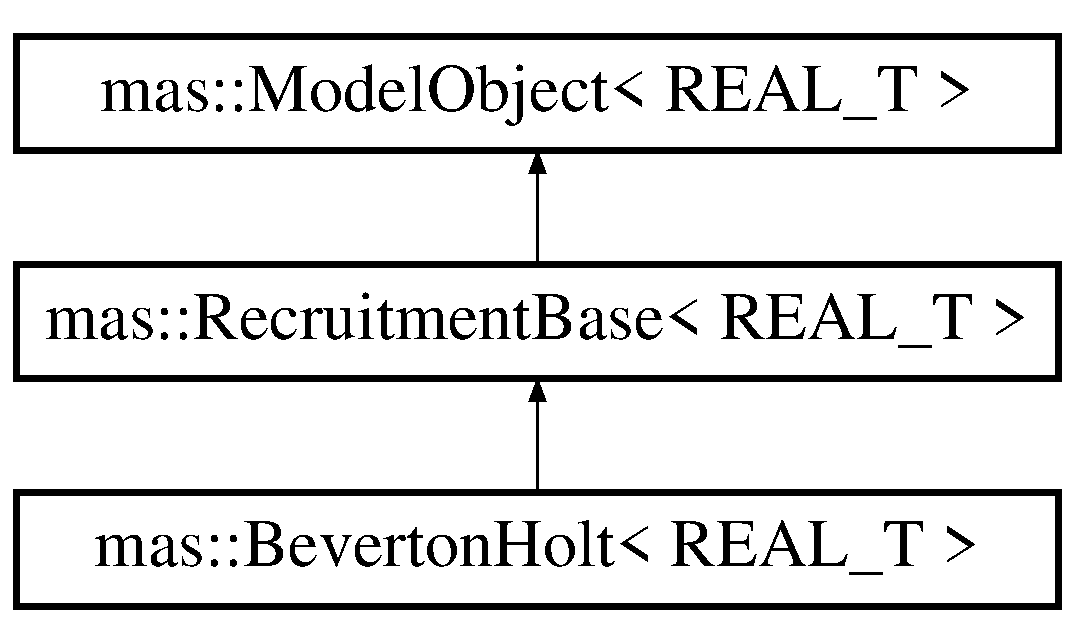
\includegraphics[height=3.000000cm]{structmas_1_1_beverton_holt}
\end{center}
\end{figure}
\subsection*{Public Types}
\begin{DoxyCompactItemize}
\item 
typedef \hyperlink{structmas_1_1_variable_trait}{Variable\-Trait}$<$ R\-E\-A\-L\-\_\-\-T $>$\\*
\-::\hyperlink{structmas_1_1_beverton_holt_af5114ac8a1dceb03a3148bd6ad7ea57a}{variable} \hyperlink{structmas_1_1_beverton_holt_af5114ac8a1dceb03a3148bd6ad7ea57a}{variable}
\end{DoxyCompactItemize}
\subsection*{Public Member Functions}
\begin{DoxyCompactItemize}
\item 
const \hyperlink{structmas_1_1_beverton_holt_af5114ac8a1dceb03a3148bd6ad7ea57a}{variable} \hyperlink{structmas_1_1_beverton_holt_a2fbd4bf3841b23145fc9000fac124818}{Evaluate} (const int \&pop\-\_\-id, const int \&area\-\_\-id, const \hyperlink{structmas_1_1_beverton_holt_af5114ac8a1dceb03a3148bd6ad7ea57a}{variable} \&s)
\item 
virtual const std\-::string \hyperlink{structmas_1_1_beverton_holt_a273d2704a4974d3fdbb9287ad0984b69}{To\-J\-S\-O\-N\-String} ()
\item 
virtual const std\-::string \hyperlink{structmas_1_1_beverton_holt_aa6e6f7fa8edecf211eedee2d2219c3ce}{Name} ()
\end{DoxyCompactItemize}
\subsection*{Public Attributes}
\begin{DoxyCompactItemize}
\item 
\hyperlink{structmas_1_1_beverton_holt_af5114ac8a1dceb03a3148bd6ad7ea57a}{variable} \hyperlink{structmas_1_1_beverton_holt_a65bb63b6533d0a0e71d2b38881664d82}{alpha}
\item 
\hyperlink{structmas_1_1_beverton_holt_af5114ac8a1dceb03a3148bd6ad7ea57a}{variable} \hyperlink{structmas_1_1_beverton_holt_a7a6d8c56eb129b679ceb6d8a4e566fc4}{beta}
\end{DoxyCompactItemize}


\subsection{Detailed Description}
\subsubsection*{template$<$typename R\-E\-A\-L\-\_\-\-T$>$struct mas\-::\-Beverton\-Holt$<$ R\-E\-A\-L\-\_\-\-T $>$}



Definition at line 167 of file Recruitment.\-hpp.



\subsection{Member Typedef Documentation}
\hypertarget{structmas_1_1_beverton_holt_af5114ac8a1dceb03a3148bd6ad7ea57a}{\index{mas\-::\-Beverton\-Holt@{mas\-::\-Beverton\-Holt}!variable@{variable}}
\index{variable@{variable}!mas::BevertonHolt@{mas\-::\-Beverton\-Holt}}
\subsubsection[{variable}]{\setlength{\rightskip}{0pt plus 5cm}template$<$typename R\-E\-A\-L\-\_\-\-T $>$ typedef {\bf Variable\-Trait}$<$R\-E\-A\-L\-\_\-\-T$>$\-::{\bf variable} {\bf mas\-::\-Beverton\-Holt}$<$ R\-E\-A\-L\-\_\-\-T $>$\-::{\bf variable}}}\label{structmas_1_1_beverton_holt_af5114ac8a1dceb03a3148bd6ad7ea57a}


Definition at line 168 of file Recruitment.\-hpp.



\subsection{Member Function Documentation}
\hypertarget{structmas_1_1_beverton_holt_a2fbd4bf3841b23145fc9000fac124818}{\index{mas\-::\-Beverton\-Holt@{mas\-::\-Beverton\-Holt}!Evaluate@{Evaluate}}
\index{Evaluate@{Evaluate}!mas::BevertonHolt@{mas\-::\-Beverton\-Holt}}
\subsubsection[{Evaluate}]{\setlength{\rightskip}{0pt plus 5cm}template$<$typename R\-E\-A\-L\-\_\-\-T $>$ const {\bf variable} {\bf mas\-::\-Beverton\-Holt}$<$ R\-E\-A\-L\-\_\-\-T $>$\-::Evaluate (
\begin{DoxyParamCaption}
\item[{const int \&}]{pop\-\_\-id, }
\item[{const int \&}]{area\-\_\-id, }
\item[{const {\bf variable} \&}]{s}
\end{DoxyParamCaption}
)\hspace{0.3cm}{\ttfamily [inline]}, {\ttfamily [virtual]}}}\label{structmas_1_1_beverton_holt_a2fbd4bf3841b23145fc9000fac124818}
Beverton-\/\-Holt Spawn-\/\-Recruit relationship


\begin{DoxyParams}{Parameters}
{\em s} & -\/ spawning biomass or abundance \\
\hline
\end{DoxyParams}
\begin{DoxyReturn}{Returns}

\end{DoxyReturn}


Implements \hyperlink{structmas_1_1_recruitment_base_a74a7f9dd7090f156c6a5068ce29f53ff}{mas\-::\-Recruitment\-Base$<$ R\-E\-A\-L\-\_\-\-T $>$}.



Definition at line 178 of file Recruitment.\-hpp.

\hypertarget{structmas_1_1_beverton_holt_aa6e6f7fa8edecf211eedee2d2219c3ce}{\index{mas\-::\-Beverton\-Holt@{mas\-::\-Beverton\-Holt}!Name@{Name}}
\index{Name@{Name}!mas::BevertonHolt@{mas\-::\-Beverton\-Holt}}
\subsubsection[{Name}]{\setlength{\rightskip}{0pt plus 5cm}template$<$typename R\-E\-A\-L\-\_\-\-T $>$ virtual const std\-::string {\bf mas\-::\-Beverton\-Holt}$<$ R\-E\-A\-L\-\_\-\-T $>$\-::Name (
\begin{DoxyParamCaption}
{}
\end{DoxyParamCaption}
)\hspace{0.3cm}{\ttfamily [inline]}, {\ttfamily [virtual]}}}\label{structmas_1_1_beverton_holt_aa6e6f7fa8edecf211eedee2d2219c3ce}


Reimplemented from \hyperlink{structmas_1_1_recruitment_base_abfdd47e97127a35f81d441ac3e1afaec}{mas\-::\-Recruitment\-Base$<$ R\-E\-A\-L\-\_\-\-T $>$}.



Definition at line 201 of file Recruitment.\-hpp.

\hypertarget{structmas_1_1_beverton_holt_a273d2704a4974d3fdbb9287ad0984b69}{\index{mas\-::\-Beverton\-Holt@{mas\-::\-Beverton\-Holt}!To\-J\-S\-O\-N\-String@{To\-J\-S\-O\-N\-String}}
\index{To\-J\-S\-O\-N\-String@{To\-J\-S\-O\-N\-String}!mas::BevertonHolt@{mas\-::\-Beverton\-Holt}}
\subsubsection[{To\-J\-S\-O\-N\-String}]{\setlength{\rightskip}{0pt plus 5cm}template$<$typename R\-E\-A\-L\-\_\-\-T $>$ virtual const std\-::string {\bf mas\-::\-Beverton\-Holt}$<$ R\-E\-A\-L\-\_\-\-T $>$\-::To\-J\-S\-O\-N\-String (
\begin{DoxyParamCaption}
{}
\end{DoxyParamCaption}
)\hspace{0.3cm}{\ttfamily [inline]}, {\ttfamily [virtual]}}}\label{structmas_1_1_beverton_holt_a273d2704a4974d3fdbb9287ad0984b69}


Reimplemented from \hyperlink{structmas_1_1_model_object_af40b3c89b11919fc5aea21dcf1cd027b}{mas\-::\-Model\-Object$<$ R\-E\-A\-L\-\_\-\-T $>$}.



Definition at line 182 of file Recruitment.\-hpp.



\subsection{Member Data Documentation}
\hypertarget{structmas_1_1_beverton_holt_a65bb63b6533d0a0e71d2b38881664d82}{\index{mas\-::\-Beverton\-Holt@{mas\-::\-Beverton\-Holt}!alpha@{alpha}}
\index{alpha@{alpha}!mas::BevertonHolt@{mas\-::\-Beverton\-Holt}}
\subsubsection[{alpha}]{\setlength{\rightskip}{0pt plus 5cm}template$<$typename R\-E\-A\-L\-\_\-\-T $>$ {\bf variable} {\bf mas\-::\-Beverton\-Holt}$<$ R\-E\-A\-L\-\_\-\-T $>$\-::alpha}}\label{structmas_1_1_beverton_holt_a65bb63b6533d0a0e71d2b38881664d82}


Definition at line 169 of file Recruitment.\-hpp.

\hypertarget{structmas_1_1_beverton_holt_a7a6d8c56eb129b679ceb6d8a4e566fc4}{\index{mas\-::\-Beverton\-Holt@{mas\-::\-Beverton\-Holt}!beta@{beta}}
\index{beta@{beta}!mas::BevertonHolt@{mas\-::\-Beverton\-Holt}}
\subsubsection[{beta}]{\setlength{\rightskip}{0pt plus 5cm}template$<$typename R\-E\-A\-L\-\_\-\-T $>$ {\bf variable} {\bf mas\-::\-Beverton\-Holt}$<$ R\-E\-A\-L\-\_\-\-T $>$\-::beta}}\label{structmas_1_1_beverton_holt_a7a6d8c56eb129b679ceb6d8a4e566fc4}


Definition at line 170 of file Recruitment.\-hpp.



The documentation for this struct was generated from the following file\-:\begin{DoxyCompactItemize}
\item 
/home/oppy/\-Net\-Beans\-Projects/mas/\hyperlink{_recruitment_8hpp}{Recruitment.\-hpp}\end{DoxyCompactItemize}

\hypertarget{structmas_1_1_beverton_holt_alt}{\section{mas\-:\-:Beverton\-Holt\-Alt$<$ R\-E\-A\-L\-\_\-\-T $>$ Struct Template Reference}
\label{structmas_1_1_beverton_holt_alt}\index{mas\-::\-Beverton\-Holt\-Alt$<$ R\-E\-A\-L\-\_\-\-T $>$@{mas\-::\-Beverton\-Holt\-Alt$<$ R\-E\-A\-L\-\_\-\-T $>$}}
}


{\ttfamily \#include $<$Recruitment.\-hpp$>$}

Inheritance diagram for mas\-:\-:Beverton\-Holt\-Alt$<$ R\-E\-A\-L\-\_\-\-T $>$\-:\begin{figure}[H]
\begin{center}
\leavevmode
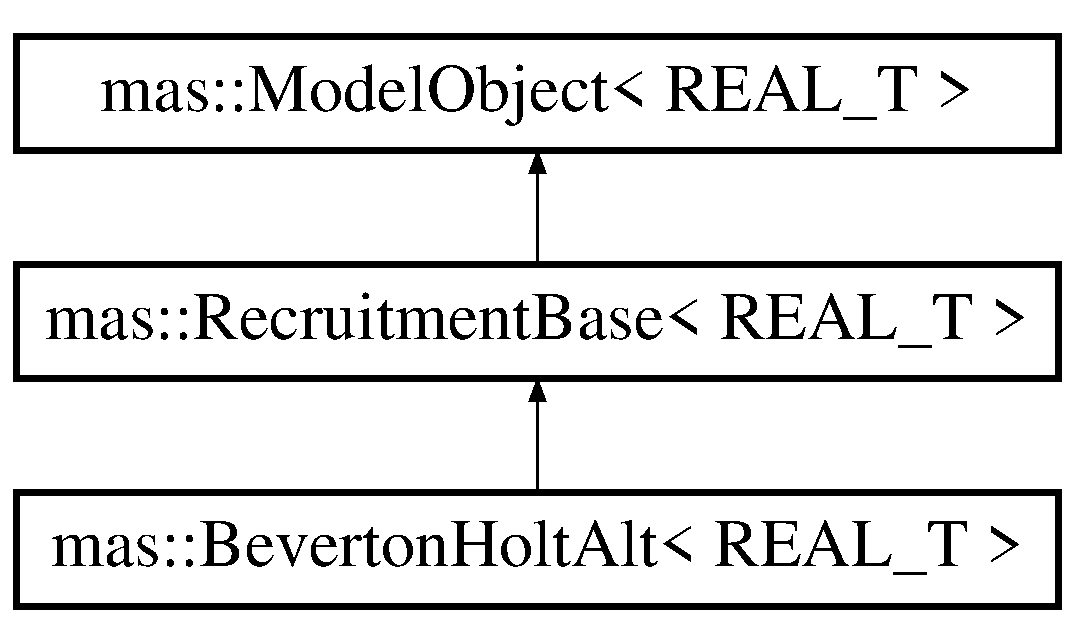
\includegraphics[height=3.000000cm]{structmas_1_1_beverton_holt_alt}
\end{center}
\end{figure}
\subsection*{Public Types}
\begin{DoxyCompactItemize}
\item 
typedef \hyperlink{structmas_1_1_variable_trait}{Variable\-Trait}$<$ R\-E\-A\-L\-\_\-\-T $>$\\*
\-::\hyperlink{structmas_1_1_model_object_a4e62fdbb5826f8fac311262b888ab10a}{variable} \hyperlink{structmas_1_1_beverton_holt_alt_a6d29c249aa28715df57bfe1d7e3c2709}{variable}
\end{DoxyCompactItemize}
\subsection*{Public Member Functions}
\begin{DoxyCompactItemize}
\item 
const \hyperlink{structmas_1_1_model_object_a4e62fdbb5826f8fac311262b888ab10a}{variable} \hyperlink{structmas_1_1_beverton_holt_alt_abce4e13656f770710ed047efa1e78ae0}{Evaluate} (const int \&pop\-\_\-id, const int \&area\-\_\-id, const \hyperlink{structmas_1_1_model_object_a4e62fdbb5826f8fac311262b888ab10a}{variable} \&s)
\item 
virtual const std\-::string \hyperlink{structmas_1_1_beverton_holt_alt_ae81da66f21c345daabf90fc7aa0db6c7}{To\-J\-S\-O\-N\-String} ()
\item 
virtual const std\-::string \hyperlink{structmas_1_1_beverton_holt_alt_a69b3da75fcea33be0ce8b12f6448b3b0}{Name} ()
\end{DoxyCompactItemize}
\subsection*{Additional Inherited Members}


\subsection{Detailed Description}
\subsubsection*{template$<$typename R\-E\-A\-L\-\_\-\-T$>$struct mas\-::\-Beverton\-Holt\-Alt$<$ R\-E\-A\-L\-\_\-\-T $>$}



Definition at line 207 of file Recruitment.\-hpp.



\subsection{Member Typedef Documentation}
\hypertarget{structmas_1_1_beverton_holt_alt_a6d29c249aa28715df57bfe1d7e3c2709}{\index{mas\-::\-Beverton\-Holt\-Alt@{mas\-::\-Beverton\-Holt\-Alt}!variable@{variable}}
\index{variable@{variable}!mas::BevertonHoltAlt@{mas\-::\-Beverton\-Holt\-Alt}}
\subsubsection[{variable}]{\setlength{\rightskip}{0pt plus 5cm}template$<$typename R\-E\-A\-L\-\_\-\-T $>$ typedef {\bf Variable\-Trait}$<$R\-E\-A\-L\-\_\-\-T$>$\-::{\bf variable} {\bf mas\-::\-Beverton\-Holt\-Alt}$<$ R\-E\-A\-L\-\_\-\-T $>$\-::{\bf variable}}}\label{structmas_1_1_beverton_holt_alt_a6d29c249aa28715df57bfe1d7e3c2709}


Definition at line 208 of file Recruitment.\-hpp.



\subsection{Member Function Documentation}
\hypertarget{structmas_1_1_beverton_holt_alt_abce4e13656f770710ed047efa1e78ae0}{\index{mas\-::\-Beverton\-Holt\-Alt@{mas\-::\-Beverton\-Holt\-Alt}!Evaluate@{Evaluate}}
\index{Evaluate@{Evaluate}!mas::BevertonHoltAlt@{mas\-::\-Beverton\-Holt\-Alt}}
\subsubsection[{Evaluate}]{\setlength{\rightskip}{0pt plus 5cm}template$<$typename R\-E\-A\-L\-\_\-\-T $>$ const {\bf variable} {\bf mas\-::\-Beverton\-Holt\-Alt}$<$ R\-E\-A\-L\-\_\-\-T $>$\-::Evaluate (
\begin{DoxyParamCaption}
\item[{const int \&}]{pop\-\_\-id, }
\item[{const int \&}]{area\-\_\-id, }
\item[{const {\bf variable} \&}]{s}
\end{DoxyParamCaption}
)\hspace{0.3cm}{\ttfamily [inline]}, {\ttfamily [virtual]}}}\label{structmas_1_1_beverton_holt_alt_abce4e13656f770710ed047efa1e78ae0}
Alternative Beverton-\/\-Holt S-\/\-R relationship


\begin{DoxyParams}{Parameters}
{\em s} & -\/ spawning biomass or abundance \\
\hline
\end{DoxyParams}
\begin{DoxyReturn}{Returns}

\end{DoxyReturn}


Implements \hyperlink{structmas_1_1_recruitment_base_a74a7f9dd7090f156c6a5068ce29f53ff}{mas\-::\-Recruitment\-Base$<$ R\-E\-A\-L\-\_\-\-T $>$}.



Definition at line 216 of file Recruitment.\-hpp.

\hypertarget{structmas_1_1_beverton_holt_alt_a69b3da75fcea33be0ce8b12f6448b3b0}{\index{mas\-::\-Beverton\-Holt\-Alt@{mas\-::\-Beverton\-Holt\-Alt}!Name@{Name}}
\index{Name@{Name}!mas::BevertonHoltAlt@{mas\-::\-Beverton\-Holt\-Alt}}
\subsubsection[{Name}]{\setlength{\rightskip}{0pt plus 5cm}template$<$typename R\-E\-A\-L\-\_\-\-T $>$ virtual const std\-::string {\bf mas\-::\-Beverton\-Holt\-Alt}$<$ R\-E\-A\-L\-\_\-\-T $>$\-::Name (
\begin{DoxyParamCaption}
{}
\end{DoxyParamCaption}
)\hspace{0.3cm}{\ttfamily [inline]}, {\ttfamily [virtual]}}}\label{structmas_1_1_beverton_holt_alt_a69b3da75fcea33be0ce8b12f6448b3b0}


Reimplemented from \hyperlink{structmas_1_1_recruitment_base_abfdd47e97127a35f81d441ac3e1afaec}{mas\-::\-Recruitment\-Base$<$ R\-E\-A\-L\-\_\-\-T $>$}.



Definition at line 245 of file Recruitment.\-hpp.

\hypertarget{structmas_1_1_beverton_holt_alt_ae81da66f21c345daabf90fc7aa0db6c7}{\index{mas\-::\-Beverton\-Holt\-Alt@{mas\-::\-Beverton\-Holt\-Alt}!To\-J\-S\-O\-N\-String@{To\-J\-S\-O\-N\-String}}
\index{To\-J\-S\-O\-N\-String@{To\-J\-S\-O\-N\-String}!mas::BevertonHoltAlt@{mas\-::\-Beverton\-Holt\-Alt}}
\subsubsection[{To\-J\-S\-O\-N\-String}]{\setlength{\rightskip}{0pt plus 5cm}template$<$typename R\-E\-A\-L\-\_\-\-T $>$ virtual const std\-::string {\bf mas\-::\-Beverton\-Holt\-Alt}$<$ R\-E\-A\-L\-\_\-\-T $>$\-::To\-J\-S\-O\-N\-String (
\begin{DoxyParamCaption}
{}
\end{DoxyParamCaption}
)\hspace{0.3cm}{\ttfamily [inline]}, {\ttfamily [virtual]}}}\label{structmas_1_1_beverton_holt_alt_ae81da66f21c345daabf90fc7aa0db6c7}


Reimplemented from \hyperlink{structmas_1_1_model_object_af40b3c89b11919fc5aea21dcf1cd027b}{mas\-::\-Model\-Object$<$ R\-E\-A\-L\-\_\-\-T $>$}.



Definition at line 228 of file Recruitment.\-hpp.



The documentation for this struct was generated from the following file\-:\begin{DoxyCompactItemize}
\item 
/home/oppy/\-Net\-Beans\-Projects/mas/\hyperlink{_recruitment_8hpp}{Recruitment.\-hpp}\end{DoxyCompactItemize}

\hypertarget{structmas_1_1_beverton_holt_dep}{\section{mas\-:\-:Beverton\-Holt\-Dep$<$ R\-E\-A\-L\-\_\-\-T $>$ Struct Template Reference}
\label{structmas_1_1_beverton_holt_dep}\index{mas\-::\-Beverton\-Holt\-Dep$<$ R\-E\-A\-L\-\_\-\-T $>$@{mas\-::\-Beverton\-Holt\-Dep$<$ R\-E\-A\-L\-\_\-\-T $>$}}
}


{\ttfamily \#include $<$Recruitment.\-hpp$>$}

Inheritance diagram for mas\-:\-:Beverton\-Holt\-Dep$<$ R\-E\-A\-L\-\_\-\-T $>$\-:\begin{figure}[H]
\begin{center}
\leavevmode
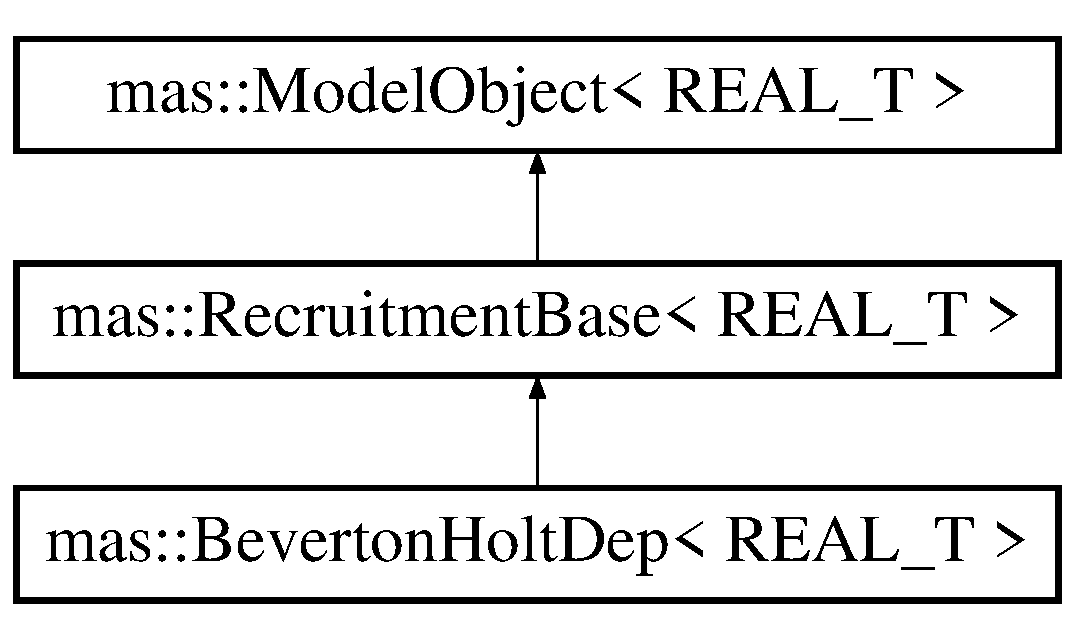
\includegraphics[height=3.000000cm]{structmas_1_1_beverton_holt_dep}
\end{center}
\end{figure}
\subsection*{Public Types}
\begin{DoxyCompactItemize}
\item 
typedef \hyperlink{structmas_1_1_variable_trait}{Variable\-Trait}$<$ R\-E\-A\-L\-\_\-\-T $>$\\*
\-::\hyperlink{structmas_1_1_beverton_holt_dep_a9d24addbd81435aa63224f31f4b96fd3}{variable} \hyperlink{structmas_1_1_beverton_holt_dep_a9d24addbd81435aa63224f31f4b96fd3}{variable}
\end{DoxyCompactItemize}
\subsection*{Public Member Functions}
\begin{DoxyCompactItemize}
\item 
const \hyperlink{structmas_1_1_beverton_holt_dep_a9d24addbd81435aa63224f31f4b96fd3}{variable} \hyperlink{structmas_1_1_beverton_holt_dep_a9433b67c120c398d05c3f900db44f985}{Evaluate} (const int \&pop\-\_\-id, const int \&area\-\_\-id, const \hyperlink{structmas_1_1_beverton_holt_dep_a9d24addbd81435aa63224f31f4b96fd3}{variable} \&s)
\item 
virtual const std\-::string \hyperlink{structmas_1_1_beverton_holt_dep_ac2af0de80fd4cc3606d8986cfa1e5781}{To\-J\-S\-O\-N\-String} ()
\item 
virtual const std\-::string \hyperlink{structmas_1_1_beverton_holt_dep_ac389fdb4eb88ccd663ec47a854d703d1}{Name} ()
\end{DoxyCompactItemize}
\subsection*{Public Attributes}
\begin{DoxyCompactItemize}
\item 
\hyperlink{structmas_1_1_beverton_holt_dep_a9d24addbd81435aa63224f31f4b96fd3}{variable} \hyperlink{structmas_1_1_beverton_holt_dep_aa3c39a19325434f7f76448365fd66744}{alpha}
\item 
\hyperlink{structmas_1_1_beverton_holt_dep_a9d24addbd81435aa63224f31f4b96fd3}{variable} \hyperlink{structmas_1_1_beverton_holt_dep_a35104d09d811c33f724b94dcad050916}{beta}
\item 
\hyperlink{structmas_1_1_beverton_holt_dep_a9d24addbd81435aa63224f31f4b96fd3}{variable} \hyperlink{structmas_1_1_beverton_holt_dep_abe85a3970eb878c0c5fd0f2a4027bb10}{c}
\end{DoxyCompactItemize}


\subsection{Detailed Description}
\subsubsection*{template$<$typename R\-E\-A\-L\-\_\-\-T$>$struct mas\-::\-Beverton\-Holt\-Dep$<$ R\-E\-A\-L\-\_\-\-T $>$}



Definition at line 251 of file Recruitment.\-hpp.



\subsection{Member Typedef Documentation}
\hypertarget{structmas_1_1_beverton_holt_dep_a9d24addbd81435aa63224f31f4b96fd3}{\index{mas\-::\-Beverton\-Holt\-Dep@{mas\-::\-Beverton\-Holt\-Dep}!variable@{variable}}
\index{variable@{variable}!mas::BevertonHoltDep@{mas\-::\-Beverton\-Holt\-Dep}}
\subsubsection[{variable}]{\setlength{\rightskip}{0pt plus 5cm}template$<$typename R\-E\-A\-L\-\_\-\-T $>$ typedef {\bf Variable\-Trait}$<$R\-E\-A\-L\-\_\-\-T$>$\-::{\bf variable} {\bf mas\-::\-Beverton\-Holt\-Dep}$<$ R\-E\-A\-L\-\_\-\-T $>$\-::{\bf variable}}}\label{structmas_1_1_beverton_holt_dep_a9d24addbd81435aa63224f31f4b96fd3}


Definition at line 252 of file Recruitment.\-hpp.



\subsection{Member Function Documentation}
\hypertarget{structmas_1_1_beverton_holt_dep_a9433b67c120c398d05c3f900db44f985}{\index{mas\-::\-Beverton\-Holt\-Dep@{mas\-::\-Beverton\-Holt\-Dep}!Evaluate@{Evaluate}}
\index{Evaluate@{Evaluate}!mas::BevertonHoltDep@{mas\-::\-Beverton\-Holt\-Dep}}
\subsubsection[{Evaluate}]{\setlength{\rightskip}{0pt plus 5cm}template$<$typename R\-E\-A\-L\-\_\-\-T $>$ const {\bf variable} {\bf mas\-::\-Beverton\-Holt\-Dep}$<$ R\-E\-A\-L\-\_\-\-T $>$\-::Evaluate (
\begin{DoxyParamCaption}
\item[{const int \&}]{pop\-\_\-id, }
\item[{const int \&}]{area\-\_\-id, }
\item[{const {\bf variable} \&}]{s}
\end{DoxyParamCaption}
)\hspace{0.3cm}{\ttfamily [inline]}, {\ttfamily [virtual]}}}\label{structmas_1_1_beverton_holt_dep_a9433b67c120c398d05c3f900db44f985}
Depensatory Beverton-\/\-Holt S-\/\-R relationship


\begin{DoxyParams}{Parameters}
{\em s} & -\/ spawning biomass or abundance \\
\hline
\end{DoxyParams}
\begin{DoxyReturn}{Returns}

\end{DoxyReturn}


Implements \hyperlink{structmas_1_1_recruitment_base_a74a7f9dd7090f156c6a5068ce29f53ff}{mas\-::\-Recruitment\-Base$<$ R\-E\-A\-L\-\_\-\-T $>$}.



Definition at line 263 of file Recruitment.\-hpp.

\hypertarget{structmas_1_1_beverton_holt_dep_ac389fdb4eb88ccd663ec47a854d703d1}{\index{mas\-::\-Beverton\-Holt\-Dep@{mas\-::\-Beverton\-Holt\-Dep}!Name@{Name}}
\index{Name@{Name}!mas::BevertonHoltDep@{mas\-::\-Beverton\-Holt\-Dep}}
\subsubsection[{Name}]{\setlength{\rightskip}{0pt plus 5cm}template$<$typename R\-E\-A\-L\-\_\-\-T $>$ virtual const std\-::string {\bf mas\-::\-Beverton\-Holt\-Dep}$<$ R\-E\-A\-L\-\_\-\-T $>$\-::Name (
\begin{DoxyParamCaption}
{}
\end{DoxyParamCaption}
)\hspace{0.3cm}{\ttfamily [inline]}, {\ttfamily [virtual]}}}\label{structmas_1_1_beverton_holt_dep_ac389fdb4eb88ccd663ec47a854d703d1}


Reimplemented from \hyperlink{structmas_1_1_recruitment_base_abfdd47e97127a35f81d441ac3e1afaec}{mas\-::\-Recruitment\-Base$<$ R\-E\-A\-L\-\_\-\-T $>$}.



Definition at line 288 of file Recruitment.\-hpp.

\hypertarget{structmas_1_1_beverton_holt_dep_ac2af0de80fd4cc3606d8986cfa1e5781}{\index{mas\-::\-Beverton\-Holt\-Dep@{mas\-::\-Beverton\-Holt\-Dep}!To\-J\-S\-O\-N\-String@{To\-J\-S\-O\-N\-String}}
\index{To\-J\-S\-O\-N\-String@{To\-J\-S\-O\-N\-String}!mas::BevertonHoltDep@{mas\-::\-Beverton\-Holt\-Dep}}
\subsubsection[{To\-J\-S\-O\-N\-String}]{\setlength{\rightskip}{0pt plus 5cm}template$<$typename R\-E\-A\-L\-\_\-\-T $>$ virtual const std\-::string {\bf mas\-::\-Beverton\-Holt\-Dep}$<$ R\-E\-A\-L\-\_\-\-T $>$\-::To\-J\-S\-O\-N\-String (
\begin{DoxyParamCaption}
{}
\end{DoxyParamCaption}
)\hspace{0.3cm}{\ttfamily [inline]}, {\ttfamily [virtual]}}}\label{structmas_1_1_beverton_holt_dep_ac2af0de80fd4cc3606d8986cfa1e5781}


Reimplemented from \hyperlink{structmas_1_1_model_object_af40b3c89b11919fc5aea21dcf1cd027b}{mas\-::\-Model\-Object$<$ R\-E\-A\-L\-\_\-\-T $>$}.



Definition at line 268 of file Recruitment.\-hpp.



\subsection{Member Data Documentation}
\hypertarget{structmas_1_1_beverton_holt_dep_aa3c39a19325434f7f76448365fd66744}{\index{mas\-::\-Beverton\-Holt\-Dep@{mas\-::\-Beverton\-Holt\-Dep}!alpha@{alpha}}
\index{alpha@{alpha}!mas::BevertonHoltDep@{mas\-::\-Beverton\-Holt\-Dep}}
\subsubsection[{alpha}]{\setlength{\rightskip}{0pt plus 5cm}template$<$typename R\-E\-A\-L\-\_\-\-T $>$ {\bf variable} {\bf mas\-::\-Beverton\-Holt\-Dep}$<$ R\-E\-A\-L\-\_\-\-T $>$\-::alpha}}\label{structmas_1_1_beverton_holt_dep_aa3c39a19325434f7f76448365fd66744}


Definition at line 253 of file Recruitment.\-hpp.

\hypertarget{structmas_1_1_beverton_holt_dep_a35104d09d811c33f724b94dcad050916}{\index{mas\-::\-Beverton\-Holt\-Dep@{mas\-::\-Beverton\-Holt\-Dep}!beta@{beta}}
\index{beta@{beta}!mas::BevertonHoltDep@{mas\-::\-Beverton\-Holt\-Dep}}
\subsubsection[{beta}]{\setlength{\rightskip}{0pt plus 5cm}template$<$typename R\-E\-A\-L\-\_\-\-T $>$ {\bf variable} {\bf mas\-::\-Beverton\-Holt\-Dep}$<$ R\-E\-A\-L\-\_\-\-T $>$\-::beta}}\label{structmas_1_1_beverton_holt_dep_a35104d09d811c33f724b94dcad050916}


Definition at line 254 of file Recruitment.\-hpp.

\hypertarget{structmas_1_1_beverton_holt_dep_abe85a3970eb878c0c5fd0f2a4027bb10}{\index{mas\-::\-Beverton\-Holt\-Dep@{mas\-::\-Beverton\-Holt\-Dep}!c@{c}}
\index{c@{c}!mas::BevertonHoltDep@{mas\-::\-Beverton\-Holt\-Dep}}
\subsubsection[{c}]{\setlength{\rightskip}{0pt plus 5cm}template$<$typename R\-E\-A\-L\-\_\-\-T $>$ {\bf variable} {\bf mas\-::\-Beverton\-Holt\-Dep}$<$ R\-E\-A\-L\-\_\-\-T $>$\-::c}}\label{structmas_1_1_beverton_holt_dep_abe85a3970eb878c0c5fd0f2a4027bb10}


Definition at line 255 of file Recruitment.\-hpp.



The documentation for this struct was generated from the following file\-:\begin{DoxyCompactItemize}
\item 
/home/oppy/\-Net\-Beans\-Projects/mas/\hyperlink{_recruitment_8hpp}{Recruitment.\-hpp}\end{DoxyCompactItemize}

\hypertarget{structmas_1_1_data_object}{\section{mas\-:\-:Data\-Object$<$ R\-E\-A\-L\-\_\-\-T $>$ Struct Template Reference}
\label{structmas_1_1_data_object}\index{mas\-::\-Data\-Object$<$ R\-E\-A\-L\-\_\-\-T $>$@{mas\-::\-Data\-Object$<$ R\-E\-A\-L\-\_\-\-T $>$}}
}


{\ttfamily \#include $<$Common.\-hpp$>$}

\subsection*{Public Member Functions}
\begin{DoxyCompactItemize}
\item 
size\-\_\-t \hyperlink{structmas_1_1_data_object_add2f5e6a1dd101fb5b970a80a3cc539c}{get\-\_\-size} ()
\item 
R\-E\-A\-L\-\_\-\-T \& \hyperlink{structmas_1_1_data_object_ab75fa55e21c8dff0dccbc0db5f736a45}{get} (int i)
\item 
R\-E\-A\-L\-\_\-\-T \& \hyperlink{structmas_1_1_data_object_a99f5ea23dc40ff5bac4b37eab38a5353}{get} (int i, int j)
\item 
R\-E\-A\-L\-\_\-\-T \& \hyperlink{structmas_1_1_data_object_ad90d43d9bd0d663675f09fce75045232}{get} (int i, int j, int k)
\item 
R\-E\-A\-L\-\_\-\-T \& \hyperlink{structmas_1_1_data_object_a167ac06a0911247fec75855a04dcc020}{get} (int i, int j, int k, int l)
\item 
R\-E\-A\-L\-\_\-\-T \& \hyperlink{structmas_1_1_data_object_a3c5e49fb656a85a37d25aaffe8f3f1db}{get} (int i, int j, int k, int l, int m)
\item 
R\-E\-A\-L\-\_\-\-T \& \hyperlink{structmas_1_1_data_object_a005d119a6238683e259e1c8a9eade1f7}{get} (int i, int j, int k, int l, int m, int n)
\item 
R\-E\-A\-L\-\_\-\-T \& \hyperlink{structmas_1_1_data_object_a71808336487899af5c16fedebbdd32c0}{get\-\_\-error} (int i)
\item 
R\-E\-A\-L\-\_\-\-T \& \hyperlink{structmas_1_1_data_object_ad19317a28681164636741be652262c48}{get\-\_\-error} (int i, int j)
\item 
R\-E\-A\-L\-\_\-\-T \& \hyperlink{structmas_1_1_data_object_a89ed630b477a3a54caf61c9004d37ed9}{get\-\_\-error} (int i, int j, int k)
\item 
R\-E\-A\-L\-\_\-\-T \& \hyperlink{structmas_1_1_data_object_a1682f9c442a8254cd4083822b654d92d}{get\-\_\-error} (int i, int j, int k, int l)
\item 
R\-E\-A\-L\-\_\-\-T \& \hyperlink{structmas_1_1_data_object_a74530ddb39b14d7b2510da8d9f53701e}{get\-\_\-error} (int i, int j, int k, int l, int m)
\item 
R\-E\-A\-L\-\_\-\-T \& \hyperlink{structmas_1_1_data_object_ac58995528d64677e1434d4e47a7a13c3}{get\-\_\-error} (int i, int j, int k, int l, int m, int n)
\end{DoxyCompactItemize}
\subsection*{Static Public Member Functions}
\begin{DoxyCompactItemize}
\item 
static \hyperlink{namespacemas_a7e15982b9bc2fc35b571bceea4f85a6b}{Data\-Units} \hyperlink{structmas_1_1_data_object_a9da63af7bf2f0777350de9ffb5001c1a}{Get\-Units} (const std\-::string \&str)
\item 
static \hyperlink{namespacemas_a177aaabcef4ec0c3f390a7c9f6ad563b}{Fish\-Sex\-Type} \hyperlink{structmas_1_1_data_object_ab4075e8fbd70a451fb6bf370a28e9c79}{Get\-Sex} (const std\-::string \&str)
\item 
static \hyperlink{namespacemas_a011cdbd288b3370538941f20c874de27}{Data\-Object\-Type} \hyperlink{structmas_1_1_data_object_aea6931b57dcd43a63ebf7e9139116b8b}{Get\-Type} (const std\-::string \&str)
\end{DoxyCompactItemize}
\subsection*{Public Attributes}
\begin{DoxyCompactItemize}
\item 
std\-::vector$<$ R\-E\-A\-L\-\_\-\-T $>$ \hyperlink{structmas_1_1_data_object_afe358cb0a24648f460aab025b8d84cfa}{data}
\item 
std\-::vector$<$ R\-E\-A\-L\-\_\-\-T $>$ \hyperlink{structmas_1_1_data_object_a030964e2f8db36cc6e9caa251c74eac5}{observation\-\_\-error}
\item 
\hyperlink{namespacemas_a011cdbd288b3370538941f20c874de27}{Data\-Object\-Type} \hyperlink{structmas_1_1_data_object_a7cb55ace324439fd5c669d9c9e8bdb41}{type}
\item 
\hyperlink{namespacemas_a177aaabcef4ec0c3f390a7c9f6ad563b}{Fish\-Sex\-Type} \hyperlink{structmas_1_1_data_object_a33c8e663026364c72e23fa5d17b924e3}{sex\-\_\-type}
\item 
\hyperlink{namespacemas_a7e15982b9bc2fc35b571bceea4f85a6b}{Data\-Units} \hyperlink{structmas_1_1_data_object_a110ce699c4ed8de93533118b35927413}{units}
\item 
std\-::string \hyperlink{structmas_1_1_data_object_aa8aa73fed0094e9eb06dcc9aff390908}{name}
\item 
R\-E\-A\-L\-\_\-\-T \hyperlink{structmas_1_1_data_object_a02a3810366fbf0a3732e8dd84d80f39e}{missing\-\_\-value}
\item 
uint32\-\_\-t \hyperlink{structmas_1_1_data_object_abd3f89ad1237a3c419b2b9890f4236b2}{id}
\item 
uint32\-\_\-t \hyperlink{structmas_1_1_data_object_a58e3f9b4cf341c63024ee00b32bbe524}{area\-\_\-id}
\item 
uint32\-\_\-t \hyperlink{structmas_1_1_data_object_ae60deac02bbbc9ca0b0fc0faf8b34ce5}{population\-\_\-id}
\item 
uint32\-\_\-t \hyperlink{structmas_1_1_data_object_af16f06b92cad5470eee7d190ec0ffac9}{dimensions}
\item 
size\-\_\-t \hyperlink{structmas_1_1_data_object_a6249505c68ed35ad5e11c4cafd8eaa86}{imax} = 1
\item 
size\-\_\-t \hyperlink{structmas_1_1_data_object_aef9f72f453df6f2796e415306cee441e}{jmax} = 1
\item 
size\-\_\-t \hyperlink{structmas_1_1_data_object_a01bdbd0efce9891dac23e3beb746e2a9}{kmax} = 1
\item 
size\-\_\-t \hyperlink{structmas_1_1_data_object_a5b9a9d140f5378c98c10c1abd0c89bbc}{lmax} = 1
\item 
size\-\_\-t \hyperlink{structmas_1_1_data_object_aad1fab74aa21aaed012c6d50a77a8077}{mmax} = 1
\item 
size\-\_\-t \hyperlink{structmas_1_1_data_object_aee973c338436ee4ee27a23a4bd855286}{nmax} = 1
\end{DoxyCompactItemize}


\subsection{Detailed Description}
\subsubsection*{template$<$typename R\-E\-A\-L\-\_\-\-T$>$struct mas\-::\-Data\-Object$<$ R\-E\-A\-L\-\_\-\-T $>$}



Definition at line 138 of file Common.\-hpp.



\subsection{Member Function Documentation}
\hypertarget{structmas_1_1_data_object_ab75fa55e21c8dff0dccbc0db5f736a45}{\index{mas\-::\-Data\-Object@{mas\-::\-Data\-Object}!get@{get}}
\index{get@{get}!mas::DataObject@{mas\-::\-Data\-Object}}
\subsubsection[{get}]{\setlength{\rightskip}{0pt plus 5cm}template$<$typename R\-E\-A\-L\-\_\-\-T $>$ R\-E\-A\-L\-\_\-\-T\& {\bf mas\-::\-Data\-Object}$<$ R\-E\-A\-L\-\_\-\-T $>$\-::get (
\begin{DoxyParamCaption}
\item[{int}]{i}
\end{DoxyParamCaption}
)\hspace{0.3cm}{\ttfamily [inline]}}}\label{structmas_1_1_data_object_ab75fa55e21c8dff0dccbc0db5f736a45}


Definition at line 162 of file Common.\-hpp.

\hypertarget{structmas_1_1_data_object_a99f5ea23dc40ff5bac4b37eab38a5353}{\index{mas\-::\-Data\-Object@{mas\-::\-Data\-Object}!get@{get}}
\index{get@{get}!mas::DataObject@{mas\-::\-Data\-Object}}
\subsubsection[{get}]{\setlength{\rightskip}{0pt plus 5cm}template$<$typename R\-E\-A\-L\-\_\-\-T $>$ R\-E\-A\-L\-\_\-\-T\& {\bf mas\-::\-Data\-Object}$<$ R\-E\-A\-L\-\_\-\-T $>$\-::get (
\begin{DoxyParamCaption}
\item[{int}]{i, }
\item[{int}]{j}
\end{DoxyParamCaption}
)\hspace{0.3cm}{\ttfamily [inline]}}}\label{structmas_1_1_data_object_a99f5ea23dc40ff5bac4b37eab38a5353}


Definition at line 166 of file Common.\-hpp.

\hypertarget{structmas_1_1_data_object_ad90d43d9bd0d663675f09fce75045232}{\index{mas\-::\-Data\-Object@{mas\-::\-Data\-Object}!get@{get}}
\index{get@{get}!mas::DataObject@{mas\-::\-Data\-Object}}
\subsubsection[{get}]{\setlength{\rightskip}{0pt plus 5cm}template$<$typename R\-E\-A\-L\-\_\-\-T $>$ R\-E\-A\-L\-\_\-\-T\& {\bf mas\-::\-Data\-Object}$<$ R\-E\-A\-L\-\_\-\-T $>$\-::get (
\begin{DoxyParamCaption}
\item[{int}]{i, }
\item[{int}]{j, }
\item[{int}]{k}
\end{DoxyParamCaption}
)\hspace{0.3cm}{\ttfamily [inline]}}}\label{structmas_1_1_data_object_ad90d43d9bd0d663675f09fce75045232}


Definition at line 170 of file Common.\-hpp.

\hypertarget{structmas_1_1_data_object_a167ac06a0911247fec75855a04dcc020}{\index{mas\-::\-Data\-Object@{mas\-::\-Data\-Object}!get@{get}}
\index{get@{get}!mas::DataObject@{mas\-::\-Data\-Object}}
\subsubsection[{get}]{\setlength{\rightskip}{0pt plus 5cm}template$<$typename R\-E\-A\-L\-\_\-\-T $>$ R\-E\-A\-L\-\_\-\-T\& {\bf mas\-::\-Data\-Object}$<$ R\-E\-A\-L\-\_\-\-T $>$\-::get (
\begin{DoxyParamCaption}
\item[{int}]{i, }
\item[{int}]{j, }
\item[{int}]{k, }
\item[{int}]{l}
\end{DoxyParamCaption}
)\hspace{0.3cm}{\ttfamily [inline]}}}\label{structmas_1_1_data_object_a167ac06a0911247fec75855a04dcc020}


Definition at line 174 of file Common.\-hpp.

\hypertarget{structmas_1_1_data_object_a3c5e49fb656a85a37d25aaffe8f3f1db}{\index{mas\-::\-Data\-Object@{mas\-::\-Data\-Object}!get@{get}}
\index{get@{get}!mas::DataObject@{mas\-::\-Data\-Object}}
\subsubsection[{get}]{\setlength{\rightskip}{0pt plus 5cm}template$<$typename R\-E\-A\-L\-\_\-\-T $>$ R\-E\-A\-L\-\_\-\-T\& {\bf mas\-::\-Data\-Object}$<$ R\-E\-A\-L\-\_\-\-T $>$\-::get (
\begin{DoxyParamCaption}
\item[{int}]{i, }
\item[{int}]{j, }
\item[{int}]{k, }
\item[{int}]{l, }
\item[{int}]{m}
\end{DoxyParamCaption}
)\hspace{0.3cm}{\ttfamily [inline]}}}\label{structmas_1_1_data_object_a3c5e49fb656a85a37d25aaffe8f3f1db}


Definition at line 178 of file Common.\-hpp.

\hypertarget{structmas_1_1_data_object_a005d119a6238683e259e1c8a9eade1f7}{\index{mas\-::\-Data\-Object@{mas\-::\-Data\-Object}!get@{get}}
\index{get@{get}!mas::DataObject@{mas\-::\-Data\-Object}}
\subsubsection[{get}]{\setlength{\rightskip}{0pt plus 5cm}template$<$typename R\-E\-A\-L\-\_\-\-T $>$ R\-E\-A\-L\-\_\-\-T\& {\bf mas\-::\-Data\-Object}$<$ R\-E\-A\-L\-\_\-\-T $>$\-::get (
\begin{DoxyParamCaption}
\item[{int}]{i, }
\item[{int}]{j, }
\item[{int}]{k, }
\item[{int}]{l, }
\item[{int}]{m, }
\item[{int}]{n}
\end{DoxyParamCaption}
)\hspace{0.3cm}{\ttfamily [inline]}}}\label{structmas_1_1_data_object_a005d119a6238683e259e1c8a9eade1f7}


Definition at line 182 of file Common.\-hpp.

\hypertarget{structmas_1_1_data_object_a71808336487899af5c16fedebbdd32c0}{\index{mas\-::\-Data\-Object@{mas\-::\-Data\-Object}!get\-\_\-error@{get\-\_\-error}}
\index{get\-\_\-error@{get\-\_\-error}!mas::DataObject@{mas\-::\-Data\-Object}}
\subsubsection[{get\-\_\-error}]{\setlength{\rightskip}{0pt plus 5cm}template$<$typename R\-E\-A\-L\-\_\-\-T $>$ R\-E\-A\-L\-\_\-\-T\& {\bf mas\-::\-Data\-Object}$<$ R\-E\-A\-L\-\_\-\-T $>$\-::get\-\_\-error (
\begin{DoxyParamCaption}
\item[{int}]{i}
\end{DoxyParamCaption}
)\hspace{0.3cm}{\ttfamily [inline]}}}\label{structmas_1_1_data_object_a71808336487899af5c16fedebbdd32c0}


Definition at line 186 of file Common.\-hpp.

\hypertarget{structmas_1_1_data_object_ad19317a28681164636741be652262c48}{\index{mas\-::\-Data\-Object@{mas\-::\-Data\-Object}!get\-\_\-error@{get\-\_\-error}}
\index{get\-\_\-error@{get\-\_\-error}!mas::DataObject@{mas\-::\-Data\-Object}}
\subsubsection[{get\-\_\-error}]{\setlength{\rightskip}{0pt plus 5cm}template$<$typename R\-E\-A\-L\-\_\-\-T $>$ R\-E\-A\-L\-\_\-\-T\& {\bf mas\-::\-Data\-Object}$<$ R\-E\-A\-L\-\_\-\-T $>$\-::get\-\_\-error (
\begin{DoxyParamCaption}
\item[{int}]{i, }
\item[{int}]{j}
\end{DoxyParamCaption}
)\hspace{0.3cm}{\ttfamily [inline]}}}\label{structmas_1_1_data_object_ad19317a28681164636741be652262c48}


Definition at line 190 of file Common.\-hpp.

\hypertarget{structmas_1_1_data_object_a89ed630b477a3a54caf61c9004d37ed9}{\index{mas\-::\-Data\-Object@{mas\-::\-Data\-Object}!get\-\_\-error@{get\-\_\-error}}
\index{get\-\_\-error@{get\-\_\-error}!mas::DataObject@{mas\-::\-Data\-Object}}
\subsubsection[{get\-\_\-error}]{\setlength{\rightskip}{0pt plus 5cm}template$<$typename R\-E\-A\-L\-\_\-\-T $>$ R\-E\-A\-L\-\_\-\-T\& {\bf mas\-::\-Data\-Object}$<$ R\-E\-A\-L\-\_\-\-T $>$\-::get\-\_\-error (
\begin{DoxyParamCaption}
\item[{int}]{i, }
\item[{int}]{j, }
\item[{int}]{k}
\end{DoxyParamCaption}
)\hspace{0.3cm}{\ttfamily [inline]}}}\label{structmas_1_1_data_object_a89ed630b477a3a54caf61c9004d37ed9}


Definition at line 194 of file Common.\-hpp.

\hypertarget{structmas_1_1_data_object_a1682f9c442a8254cd4083822b654d92d}{\index{mas\-::\-Data\-Object@{mas\-::\-Data\-Object}!get\-\_\-error@{get\-\_\-error}}
\index{get\-\_\-error@{get\-\_\-error}!mas::DataObject@{mas\-::\-Data\-Object}}
\subsubsection[{get\-\_\-error}]{\setlength{\rightskip}{0pt plus 5cm}template$<$typename R\-E\-A\-L\-\_\-\-T $>$ R\-E\-A\-L\-\_\-\-T\& {\bf mas\-::\-Data\-Object}$<$ R\-E\-A\-L\-\_\-\-T $>$\-::get\-\_\-error (
\begin{DoxyParamCaption}
\item[{int}]{i, }
\item[{int}]{j, }
\item[{int}]{k, }
\item[{int}]{l}
\end{DoxyParamCaption}
)\hspace{0.3cm}{\ttfamily [inline]}}}\label{structmas_1_1_data_object_a1682f9c442a8254cd4083822b654d92d}


Definition at line 198 of file Common.\-hpp.

\hypertarget{structmas_1_1_data_object_a74530ddb39b14d7b2510da8d9f53701e}{\index{mas\-::\-Data\-Object@{mas\-::\-Data\-Object}!get\-\_\-error@{get\-\_\-error}}
\index{get\-\_\-error@{get\-\_\-error}!mas::DataObject@{mas\-::\-Data\-Object}}
\subsubsection[{get\-\_\-error}]{\setlength{\rightskip}{0pt plus 5cm}template$<$typename R\-E\-A\-L\-\_\-\-T $>$ R\-E\-A\-L\-\_\-\-T\& {\bf mas\-::\-Data\-Object}$<$ R\-E\-A\-L\-\_\-\-T $>$\-::get\-\_\-error (
\begin{DoxyParamCaption}
\item[{int}]{i, }
\item[{int}]{j, }
\item[{int}]{k, }
\item[{int}]{l, }
\item[{int}]{m}
\end{DoxyParamCaption}
)\hspace{0.3cm}{\ttfamily [inline]}}}\label{structmas_1_1_data_object_a74530ddb39b14d7b2510da8d9f53701e}


Definition at line 202 of file Common.\-hpp.

\hypertarget{structmas_1_1_data_object_ac58995528d64677e1434d4e47a7a13c3}{\index{mas\-::\-Data\-Object@{mas\-::\-Data\-Object}!get\-\_\-error@{get\-\_\-error}}
\index{get\-\_\-error@{get\-\_\-error}!mas::DataObject@{mas\-::\-Data\-Object}}
\subsubsection[{get\-\_\-error}]{\setlength{\rightskip}{0pt plus 5cm}template$<$typename R\-E\-A\-L\-\_\-\-T $>$ R\-E\-A\-L\-\_\-\-T\& {\bf mas\-::\-Data\-Object}$<$ R\-E\-A\-L\-\_\-\-T $>$\-::get\-\_\-error (
\begin{DoxyParamCaption}
\item[{int}]{i, }
\item[{int}]{j, }
\item[{int}]{k, }
\item[{int}]{l, }
\item[{int}]{m, }
\item[{int}]{n}
\end{DoxyParamCaption}
)\hspace{0.3cm}{\ttfamily [inline]}}}\label{structmas_1_1_data_object_ac58995528d64677e1434d4e47a7a13c3}


Definition at line 206 of file Common.\-hpp.

\hypertarget{structmas_1_1_data_object_add2f5e6a1dd101fb5b970a80a3cc539c}{\index{mas\-::\-Data\-Object@{mas\-::\-Data\-Object}!get\-\_\-size@{get\-\_\-size}}
\index{get\-\_\-size@{get\-\_\-size}!mas::DataObject@{mas\-::\-Data\-Object}}
\subsubsection[{get\-\_\-size}]{\setlength{\rightskip}{0pt plus 5cm}template$<$typename R\-E\-A\-L\-\_\-\-T $>$ size\-\_\-t {\bf mas\-::\-Data\-Object}$<$ R\-E\-A\-L\-\_\-\-T $>$\-::get\-\_\-size (
\begin{DoxyParamCaption}
{}
\end{DoxyParamCaption}
)\hspace{0.3cm}{\ttfamily [inline]}}}\label{structmas_1_1_data_object_add2f5e6a1dd101fb5b970a80a3cc539c}


Definition at line 158 of file Common.\-hpp.

\hypertarget{structmas_1_1_data_object_ab4075e8fbd70a451fb6bf370a28e9c79}{\index{mas\-::\-Data\-Object@{mas\-::\-Data\-Object}!Get\-Sex@{Get\-Sex}}
\index{Get\-Sex@{Get\-Sex}!mas::DataObject@{mas\-::\-Data\-Object}}
\subsubsection[{Get\-Sex}]{\setlength{\rightskip}{0pt plus 5cm}template$<$typename R\-E\-A\-L\-\_\-\-T $>$ static {\bf Fish\-Sex\-Type} {\bf mas\-::\-Data\-Object}$<$ R\-E\-A\-L\-\_\-\-T $>$\-::Get\-Sex (
\begin{DoxyParamCaption}
\item[{const std\-::string \&}]{str}
\end{DoxyParamCaption}
)\hspace{0.3cm}{\ttfamily [inline]}, {\ttfamily [static]}}}\label{structmas_1_1_data_object_ab4075e8fbd70a451fb6bf370a28e9c79}


Definition at line 225 of file Common.\-hpp.

\hypertarget{structmas_1_1_data_object_aea6931b57dcd43a63ebf7e9139116b8b}{\index{mas\-::\-Data\-Object@{mas\-::\-Data\-Object}!Get\-Type@{Get\-Type}}
\index{Get\-Type@{Get\-Type}!mas::DataObject@{mas\-::\-Data\-Object}}
\subsubsection[{Get\-Type}]{\setlength{\rightskip}{0pt plus 5cm}template$<$typename R\-E\-A\-L\-\_\-\-T $>$ static {\bf Data\-Object\-Type} {\bf mas\-::\-Data\-Object}$<$ R\-E\-A\-L\-\_\-\-T $>$\-::Get\-Type (
\begin{DoxyParamCaption}
\item[{const std\-::string \&}]{str}
\end{DoxyParamCaption}
)\hspace{0.3cm}{\ttfamily [inline]}, {\ttfamily [static]}}}\label{structmas_1_1_data_object_aea6931b57dcd43a63ebf7e9139116b8b}


Definition at line 238 of file Common.\-hpp.

\hypertarget{structmas_1_1_data_object_a9da63af7bf2f0777350de9ffb5001c1a}{\index{mas\-::\-Data\-Object@{mas\-::\-Data\-Object}!Get\-Units@{Get\-Units}}
\index{Get\-Units@{Get\-Units}!mas::DataObject@{mas\-::\-Data\-Object}}
\subsubsection[{Get\-Units}]{\setlength{\rightskip}{0pt plus 5cm}template$<$typename R\-E\-A\-L\-\_\-\-T $>$ static {\bf Data\-Units} {\bf mas\-::\-Data\-Object}$<$ R\-E\-A\-L\-\_\-\-T $>$\-::Get\-Units (
\begin{DoxyParamCaption}
\item[{const std\-::string \&}]{str}
\end{DoxyParamCaption}
)\hspace{0.3cm}{\ttfamily [inline]}, {\ttfamily [static]}}}\label{structmas_1_1_data_object_a9da63af7bf2f0777350de9ffb5001c1a}


Definition at line 210 of file Common.\-hpp.



\subsection{Member Data Documentation}
\hypertarget{structmas_1_1_data_object_a58e3f9b4cf341c63024ee00b32bbe524}{\index{mas\-::\-Data\-Object@{mas\-::\-Data\-Object}!area\-\_\-id@{area\-\_\-id}}
\index{area\-\_\-id@{area\-\_\-id}!mas::DataObject@{mas\-::\-Data\-Object}}
\subsubsection[{area\-\_\-id}]{\setlength{\rightskip}{0pt plus 5cm}template$<$typename R\-E\-A\-L\-\_\-\-T $>$ uint32\-\_\-t {\bf mas\-::\-Data\-Object}$<$ R\-E\-A\-L\-\_\-\-T $>$\-::area\-\_\-id}}\label{structmas_1_1_data_object_a58e3f9b4cf341c63024ee00b32bbe524}


Definition at line 148 of file Common.\-hpp.

\hypertarget{structmas_1_1_data_object_afe358cb0a24648f460aab025b8d84cfa}{\index{mas\-::\-Data\-Object@{mas\-::\-Data\-Object}!data@{data}}
\index{data@{data}!mas::DataObject@{mas\-::\-Data\-Object}}
\subsubsection[{data}]{\setlength{\rightskip}{0pt plus 5cm}template$<$typename R\-E\-A\-L\-\_\-\-T $>$ std\-::vector$<$R\-E\-A\-L\-\_\-\-T$>$ {\bf mas\-::\-Data\-Object}$<$ R\-E\-A\-L\-\_\-\-T $>$\-::data}}\label{structmas_1_1_data_object_afe358cb0a24648f460aab025b8d84cfa}


Definition at line 139 of file Common.\-hpp.

\hypertarget{structmas_1_1_data_object_af16f06b92cad5470eee7d190ec0ffac9}{\index{mas\-::\-Data\-Object@{mas\-::\-Data\-Object}!dimensions@{dimensions}}
\index{dimensions@{dimensions}!mas::DataObject@{mas\-::\-Data\-Object}}
\subsubsection[{dimensions}]{\setlength{\rightskip}{0pt plus 5cm}template$<$typename R\-E\-A\-L\-\_\-\-T $>$ uint32\-\_\-t {\bf mas\-::\-Data\-Object}$<$ R\-E\-A\-L\-\_\-\-T $>$\-::dimensions}}\label{structmas_1_1_data_object_af16f06b92cad5470eee7d190ec0ffac9}


Definition at line 150 of file Common.\-hpp.

\hypertarget{structmas_1_1_data_object_abd3f89ad1237a3c419b2b9890f4236b2}{\index{mas\-::\-Data\-Object@{mas\-::\-Data\-Object}!id@{id}}
\index{id@{id}!mas::DataObject@{mas\-::\-Data\-Object}}
\subsubsection[{id}]{\setlength{\rightskip}{0pt plus 5cm}template$<$typename R\-E\-A\-L\-\_\-\-T $>$ uint32\-\_\-t {\bf mas\-::\-Data\-Object}$<$ R\-E\-A\-L\-\_\-\-T $>$\-::id}}\label{structmas_1_1_data_object_abd3f89ad1237a3c419b2b9890f4236b2}


Definition at line 147 of file Common.\-hpp.

\hypertarget{structmas_1_1_data_object_a6249505c68ed35ad5e11c4cafd8eaa86}{\index{mas\-::\-Data\-Object@{mas\-::\-Data\-Object}!imax@{imax}}
\index{imax@{imax}!mas::DataObject@{mas\-::\-Data\-Object}}
\subsubsection[{imax}]{\setlength{\rightskip}{0pt plus 5cm}template$<$typename R\-E\-A\-L\-\_\-\-T $>$ size\-\_\-t {\bf mas\-::\-Data\-Object}$<$ R\-E\-A\-L\-\_\-\-T $>$\-::imax = 1}}\label{structmas_1_1_data_object_a6249505c68ed35ad5e11c4cafd8eaa86}


Definition at line 151 of file Common.\-hpp.

\hypertarget{structmas_1_1_data_object_aef9f72f453df6f2796e415306cee441e}{\index{mas\-::\-Data\-Object@{mas\-::\-Data\-Object}!jmax@{jmax}}
\index{jmax@{jmax}!mas::DataObject@{mas\-::\-Data\-Object}}
\subsubsection[{jmax}]{\setlength{\rightskip}{0pt plus 5cm}template$<$typename R\-E\-A\-L\-\_\-\-T $>$ size\-\_\-t {\bf mas\-::\-Data\-Object}$<$ R\-E\-A\-L\-\_\-\-T $>$\-::jmax = 1}}\label{structmas_1_1_data_object_aef9f72f453df6f2796e415306cee441e}


Definition at line 152 of file Common.\-hpp.

\hypertarget{structmas_1_1_data_object_a01bdbd0efce9891dac23e3beb746e2a9}{\index{mas\-::\-Data\-Object@{mas\-::\-Data\-Object}!kmax@{kmax}}
\index{kmax@{kmax}!mas::DataObject@{mas\-::\-Data\-Object}}
\subsubsection[{kmax}]{\setlength{\rightskip}{0pt plus 5cm}template$<$typename R\-E\-A\-L\-\_\-\-T $>$ size\-\_\-t {\bf mas\-::\-Data\-Object}$<$ R\-E\-A\-L\-\_\-\-T $>$\-::kmax = 1}}\label{structmas_1_1_data_object_a01bdbd0efce9891dac23e3beb746e2a9}


Definition at line 153 of file Common.\-hpp.

\hypertarget{structmas_1_1_data_object_a5b9a9d140f5378c98c10c1abd0c89bbc}{\index{mas\-::\-Data\-Object@{mas\-::\-Data\-Object}!lmax@{lmax}}
\index{lmax@{lmax}!mas::DataObject@{mas\-::\-Data\-Object}}
\subsubsection[{lmax}]{\setlength{\rightskip}{0pt plus 5cm}template$<$typename R\-E\-A\-L\-\_\-\-T $>$ size\-\_\-t {\bf mas\-::\-Data\-Object}$<$ R\-E\-A\-L\-\_\-\-T $>$\-::lmax = 1}}\label{structmas_1_1_data_object_a5b9a9d140f5378c98c10c1abd0c89bbc}


Definition at line 154 of file Common.\-hpp.

\hypertarget{structmas_1_1_data_object_a02a3810366fbf0a3732e8dd84d80f39e}{\index{mas\-::\-Data\-Object@{mas\-::\-Data\-Object}!missing\-\_\-value@{missing\-\_\-value}}
\index{missing\-\_\-value@{missing\-\_\-value}!mas::DataObject@{mas\-::\-Data\-Object}}
\subsubsection[{missing\-\_\-value}]{\setlength{\rightskip}{0pt plus 5cm}template$<$typename R\-E\-A\-L\-\_\-\-T $>$ R\-E\-A\-L\-\_\-\-T {\bf mas\-::\-Data\-Object}$<$ R\-E\-A\-L\-\_\-\-T $>$\-::missing\-\_\-value}}\label{structmas_1_1_data_object_a02a3810366fbf0a3732e8dd84d80f39e}


Definition at line 145 of file Common.\-hpp.

\hypertarget{structmas_1_1_data_object_aad1fab74aa21aaed012c6d50a77a8077}{\index{mas\-::\-Data\-Object@{mas\-::\-Data\-Object}!mmax@{mmax}}
\index{mmax@{mmax}!mas::DataObject@{mas\-::\-Data\-Object}}
\subsubsection[{mmax}]{\setlength{\rightskip}{0pt plus 5cm}template$<$typename R\-E\-A\-L\-\_\-\-T $>$ size\-\_\-t {\bf mas\-::\-Data\-Object}$<$ R\-E\-A\-L\-\_\-\-T $>$\-::mmax = 1}}\label{structmas_1_1_data_object_aad1fab74aa21aaed012c6d50a77a8077}


Definition at line 155 of file Common.\-hpp.

\hypertarget{structmas_1_1_data_object_aa8aa73fed0094e9eb06dcc9aff390908}{\index{mas\-::\-Data\-Object@{mas\-::\-Data\-Object}!name@{name}}
\index{name@{name}!mas::DataObject@{mas\-::\-Data\-Object}}
\subsubsection[{name}]{\setlength{\rightskip}{0pt plus 5cm}template$<$typename R\-E\-A\-L\-\_\-\-T $>$ std\-::string {\bf mas\-::\-Data\-Object}$<$ R\-E\-A\-L\-\_\-\-T $>$\-::name}}\label{structmas_1_1_data_object_aa8aa73fed0094e9eb06dcc9aff390908}


Definition at line 144 of file Common.\-hpp.

\hypertarget{structmas_1_1_data_object_aee973c338436ee4ee27a23a4bd855286}{\index{mas\-::\-Data\-Object@{mas\-::\-Data\-Object}!nmax@{nmax}}
\index{nmax@{nmax}!mas::DataObject@{mas\-::\-Data\-Object}}
\subsubsection[{nmax}]{\setlength{\rightskip}{0pt plus 5cm}template$<$typename R\-E\-A\-L\-\_\-\-T $>$ size\-\_\-t {\bf mas\-::\-Data\-Object}$<$ R\-E\-A\-L\-\_\-\-T $>$\-::nmax = 1}}\label{structmas_1_1_data_object_aee973c338436ee4ee27a23a4bd855286}


Definition at line 156 of file Common.\-hpp.

\hypertarget{structmas_1_1_data_object_a030964e2f8db36cc6e9caa251c74eac5}{\index{mas\-::\-Data\-Object@{mas\-::\-Data\-Object}!observation\-\_\-error@{observation\-\_\-error}}
\index{observation\-\_\-error@{observation\-\_\-error}!mas::DataObject@{mas\-::\-Data\-Object}}
\subsubsection[{observation\-\_\-error}]{\setlength{\rightskip}{0pt plus 5cm}template$<$typename R\-E\-A\-L\-\_\-\-T $>$ std\-::vector$<$R\-E\-A\-L\-\_\-\-T$>$ {\bf mas\-::\-Data\-Object}$<$ R\-E\-A\-L\-\_\-\-T $>$\-::observation\-\_\-error}}\label{structmas_1_1_data_object_a030964e2f8db36cc6e9caa251c74eac5}


Definition at line 140 of file Common.\-hpp.

\hypertarget{structmas_1_1_data_object_ae60deac02bbbc9ca0b0fc0faf8b34ce5}{\index{mas\-::\-Data\-Object@{mas\-::\-Data\-Object}!population\-\_\-id@{population\-\_\-id}}
\index{population\-\_\-id@{population\-\_\-id}!mas::DataObject@{mas\-::\-Data\-Object}}
\subsubsection[{population\-\_\-id}]{\setlength{\rightskip}{0pt plus 5cm}template$<$typename R\-E\-A\-L\-\_\-\-T $>$ uint32\-\_\-t {\bf mas\-::\-Data\-Object}$<$ R\-E\-A\-L\-\_\-\-T $>$\-::population\-\_\-id}}\label{structmas_1_1_data_object_ae60deac02bbbc9ca0b0fc0faf8b34ce5}


Definition at line 149 of file Common.\-hpp.

\hypertarget{structmas_1_1_data_object_a33c8e663026364c72e23fa5d17b924e3}{\index{mas\-::\-Data\-Object@{mas\-::\-Data\-Object}!sex\-\_\-type@{sex\-\_\-type}}
\index{sex\-\_\-type@{sex\-\_\-type}!mas::DataObject@{mas\-::\-Data\-Object}}
\subsubsection[{sex\-\_\-type}]{\setlength{\rightskip}{0pt plus 5cm}template$<$typename R\-E\-A\-L\-\_\-\-T $>$ {\bf Fish\-Sex\-Type} {\bf mas\-::\-Data\-Object}$<$ R\-E\-A\-L\-\_\-\-T $>$\-::sex\-\_\-type}}\label{structmas_1_1_data_object_a33c8e663026364c72e23fa5d17b924e3}


Definition at line 142 of file Common.\-hpp.

\hypertarget{structmas_1_1_data_object_a7cb55ace324439fd5c669d9c9e8bdb41}{\index{mas\-::\-Data\-Object@{mas\-::\-Data\-Object}!type@{type}}
\index{type@{type}!mas::DataObject@{mas\-::\-Data\-Object}}
\subsubsection[{type}]{\setlength{\rightskip}{0pt plus 5cm}template$<$typename R\-E\-A\-L\-\_\-\-T $>$ {\bf Data\-Object\-Type} {\bf mas\-::\-Data\-Object}$<$ R\-E\-A\-L\-\_\-\-T $>$\-::type}}\label{structmas_1_1_data_object_a7cb55ace324439fd5c669d9c9e8bdb41}


Definition at line 141 of file Common.\-hpp.

\hypertarget{structmas_1_1_data_object_a110ce699c4ed8de93533118b35927413}{\index{mas\-::\-Data\-Object@{mas\-::\-Data\-Object}!units@{units}}
\index{units@{units}!mas::DataObject@{mas\-::\-Data\-Object}}
\subsubsection[{units}]{\setlength{\rightskip}{0pt plus 5cm}template$<$typename R\-E\-A\-L\-\_\-\-T $>$ {\bf Data\-Units} {\bf mas\-::\-Data\-Object}$<$ R\-E\-A\-L\-\_\-\-T $>$\-::units}}\label{structmas_1_1_data_object_a110ce699c4ed8de93533118b35927413}


Definition at line 143 of file Common.\-hpp.



The documentation for this struct was generated from the following file\-:\begin{DoxyCompactItemize}
\item 
/home/oppy/\-Net\-Beans\-Projects/mas/\hyperlink{_common_8hpp}{Common.\-hpp}\end{DoxyCompactItemize}

\hypertarget{structmas_1_1_deriso}{\section{mas\-:\-:Deriso$<$ R\-E\-A\-L\-\_\-\-T $>$ Struct Template Reference}
\label{structmas_1_1_deriso}\index{mas\-::\-Deriso$<$ R\-E\-A\-L\-\_\-\-T $>$@{mas\-::\-Deriso$<$ R\-E\-A\-L\-\_\-\-T $>$}}
}


{\ttfamily \#include $<$Recruitment.\-hpp$>$}

Inheritance diagram for mas\-:\-:Deriso$<$ R\-E\-A\-L\-\_\-\-T $>$\-:\begin{figure}[H]
\begin{center}
\leavevmode
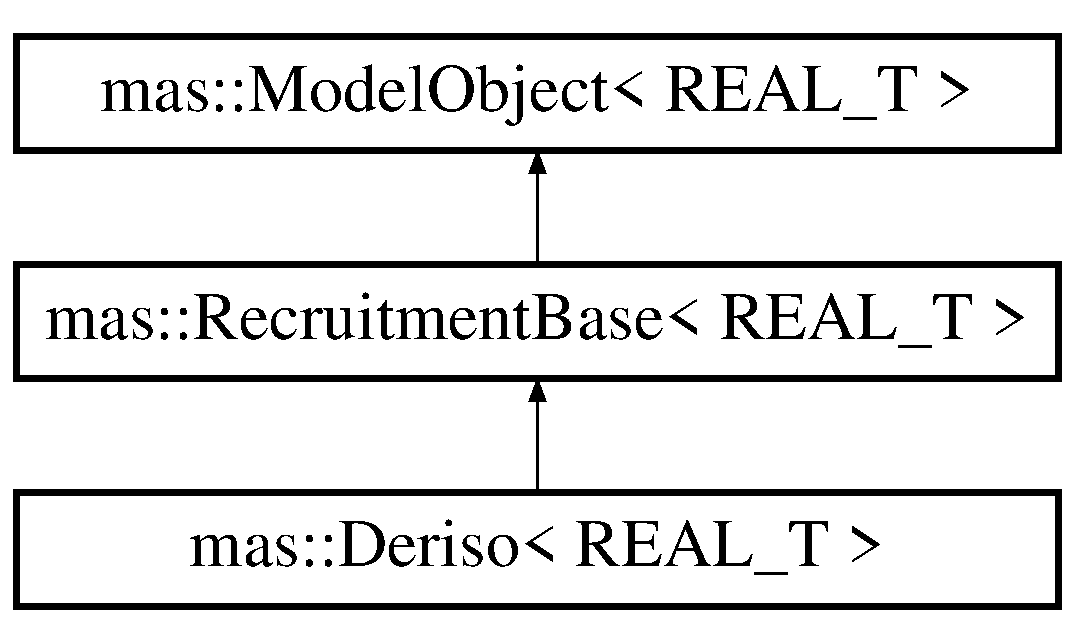
\includegraphics[height=3.000000cm]{structmas_1_1_deriso}
\end{center}
\end{figure}
\subsection*{Public Types}
\begin{DoxyCompactItemize}
\item 
typedef \hyperlink{structmas_1_1_variable_trait}{Variable\-Trait}$<$ R\-E\-A\-L\-\_\-\-T $>$\\*
\-::\hyperlink{structmas_1_1_deriso_a458705874e9be66739422da45db21ff0}{variable} \hyperlink{structmas_1_1_deriso_a458705874e9be66739422da45db21ff0}{variable}
\end{DoxyCompactItemize}
\subsection*{Public Member Functions}
\begin{DoxyCompactItemize}
\item 
const \hyperlink{structmas_1_1_deriso_a458705874e9be66739422da45db21ff0}{variable} \hyperlink{structmas_1_1_deriso_a056c98851c0b002b87c31b8b4a660fde}{Evaluate} (const int \&pop\-\_\-id, const int \&area\-\_\-id, const \hyperlink{structmas_1_1_deriso_a458705874e9be66739422da45db21ff0}{variable} \&s)
\item 
virtual const std\-::string \hyperlink{structmas_1_1_deriso_aabf1cedad5697f1924a09d3a168453c4}{To\-J\-S\-O\-N\-String} ()
\item 
virtual const std\-::string \hyperlink{structmas_1_1_deriso_a4bd2deff5d9d3cac9e90941df9881b29}{Name} ()
\end{DoxyCompactItemize}
\subsection*{Public Attributes}
\begin{DoxyCompactItemize}
\item 
\hyperlink{structmas_1_1_deriso_a458705874e9be66739422da45db21ff0}{variable} \hyperlink{structmas_1_1_deriso_a9fc2133e60c6362ac0bf4f9c18b98410}{alpha}
\item 
\hyperlink{structmas_1_1_deriso_a458705874e9be66739422da45db21ff0}{variable} \hyperlink{structmas_1_1_deriso_ae907bcd71c5768501c1eb84083e24b14}{beta}
\item 
\hyperlink{structmas_1_1_deriso_a458705874e9be66739422da45db21ff0}{variable} \hyperlink{structmas_1_1_deriso_ad1977b4273fd41597b100dcbee6c1fc0}{c}
\end{DoxyCompactItemize}


\subsection{Detailed Description}
\subsubsection*{template$<$typename R\-E\-A\-L\-\_\-\-T$>$struct mas\-::\-Deriso$<$ R\-E\-A\-L\-\_\-\-T $>$}



Definition at line 330 of file Recruitment.\-hpp.



\subsection{Member Typedef Documentation}
\hypertarget{structmas_1_1_deriso_a458705874e9be66739422da45db21ff0}{\index{mas\-::\-Deriso@{mas\-::\-Deriso}!variable@{variable}}
\index{variable@{variable}!mas::Deriso@{mas\-::\-Deriso}}
\subsubsection[{variable}]{\setlength{\rightskip}{0pt plus 5cm}template$<$typename R\-E\-A\-L\-\_\-\-T $>$ typedef {\bf Variable\-Trait}$<$R\-E\-A\-L\-\_\-\-T$>$\-::{\bf variable} {\bf mas\-::\-Deriso}$<$ R\-E\-A\-L\-\_\-\-T $>$\-::{\bf variable}}}\label{structmas_1_1_deriso_a458705874e9be66739422da45db21ff0}


Definition at line 331 of file Recruitment.\-hpp.



\subsection{Member Function Documentation}
\hypertarget{structmas_1_1_deriso_a056c98851c0b002b87c31b8b4a660fde}{\index{mas\-::\-Deriso@{mas\-::\-Deriso}!Evaluate@{Evaluate}}
\index{Evaluate@{Evaluate}!mas::Deriso@{mas\-::\-Deriso}}
\subsubsection[{Evaluate}]{\setlength{\rightskip}{0pt plus 5cm}template$<$typename R\-E\-A\-L\-\_\-\-T $>$ const {\bf variable} {\bf mas\-::\-Deriso}$<$ R\-E\-A\-L\-\_\-\-T $>$\-::Evaluate (
\begin{DoxyParamCaption}
\item[{const int \&}]{pop\-\_\-id, }
\item[{const int \&}]{area\-\_\-id, }
\item[{const {\bf variable} \&}]{s}
\end{DoxyParamCaption}
)\hspace{0.3cm}{\ttfamily [inline]}, {\ttfamily [virtual]}}}\label{structmas_1_1_deriso_a056c98851c0b002b87c31b8b4a660fde}


Implements \hyperlink{structmas_1_1_recruitment_base_a74a7f9dd7090f156c6a5068ce29f53ff}{mas\-::\-Recruitment\-Base$<$ R\-E\-A\-L\-\_\-\-T $>$}.



Definition at line 336 of file Recruitment.\-hpp.

\hypertarget{structmas_1_1_deriso_a4bd2deff5d9d3cac9e90941df9881b29}{\index{mas\-::\-Deriso@{mas\-::\-Deriso}!Name@{Name}}
\index{Name@{Name}!mas::Deriso@{mas\-::\-Deriso}}
\subsubsection[{Name}]{\setlength{\rightskip}{0pt plus 5cm}template$<$typename R\-E\-A\-L\-\_\-\-T $>$ virtual const std\-::string {\bf mas\-::\-Deriso}$<$ R\-E\-A\-L\-\_\-\-T $>$\-::Name (
\begin{DoxyParamCaption}
{}
\end{DoxyParamCaption}
)\hspace{0.3cm}{\ttfamily [inline]}, {\ttfamily [virtual]}}}\label{structmas_1_1_deriso_a4bd2deff5d9d3cac9e90941df9881b29}


Reimplemented from \hyperlink{structmas_1_1_recruitment_base_abfdd47e97127a35f81d441ac3e1afaec}{mas\-::\-Recruitment\-Base$<$ R\-E\-A\-L\-\_\-\-T $>$}.



Definition at line 360 of file Recruitment.\-hpp.

\hypertarget{structmas_1_1_deriso_aabf1cedad5697f1924a09d3a168453c4}{\index{mas\-::\-Deriso@{mas\-::\-Deriso}!To\-J\-S\-O\-N\-String@{To\-J\-S\-O\-N\-String}}
\index{To\-J\-S\-O\-N\-String@{To\-J\-S\-O\-N\-String}!mas::Deriso@{mas\-::\-Deriso}}
\subsubsection[{To\-J\-S\-O\-N\-String}]{\setlength{\rightskip}{0pt plus 5cm}template$<$typename R\-E\-A\-L\-\_\-\-T $>$ virtual const std\-::string {\bf mas\-::\-Deriso}$<$ R\-E\-A\-L\-\_\-\-T $>$\-::To\-J\-S\-O\-N\-String (
\begin{DoxyParamCaption}
{}
\end{DoxyParamCaption}
)\hspace{0.3cm}{\ttfamily [inline]}, {\ttfamily [virtual]}}}\label{structmas_1_1_deriso_aabf1cedad5697f1924a09d3a168453c4}


Reimplemented from \hyperlink{structmas_1_1_model_object_af40b3c89b11919fc5aea21dcf1cd027b}{mas\-::\-Model\-Object$<$ R\-E\-A\-L\-\_\-\-T $>$}.



Definition at line 340 of file Recruitment.\-hpp.



\subsection{Member Data Documentation}
\hypertarget{structmas_1_1_deriso_a9fc2133e60c6362ac0bf4f9c18b98410}{\index{mas\-::\-Deriso@{mas\-::\-Deriso}!alpha@{alpha}}
\index{alpha@{alpha}!mas::Deriso@{mas\-::\-Deriso}}
\subsubsection[{alpha}]{\setlength{\rightskip}{0pt plus 5cm}template$<$typename R\-E\-A\-L\-\_\-\-T $>$ {\bf variable} {\bf mas\-::\-Deriso}$<$ R\-E\-A\-L\-\_\-\-T $>$\-::alpha}}\label{structmas_1_1_deriso_a9fc2133e60c6362ac0bf4f9c18b98410}


Definition at line 332 of file Recruitment.\-hpp.

\hypertarget{structmas_1_1_deriso_ae907bcd71c5768501c1eb84083e24b14}{\index{mas\-::\-Deriso@{mas\-::\-Deriso}!beta@{beta}}
\index{beta@{beta}!mas::Deriso@{mas\-::\-Deriso}}
\subsubsection[{beta}]{\setlength{\rightskip}{0pt plus 5cm}template$<$typename R\-E\-A\-L\-\_\-\-T $>$ {\bf variable} {\bf mas\-::\-Deriso}$<$ R\-E\-A\-L\-\_\-\-T $>$\-::beta}}\label{structmas_1_1_deriso_ae907bcd71c5768501c1eb84083e24b14}


Definition at line 333 of file Recruitment.\-hpp.

\hypertarget{structmas_1_1_deriso_ad1977b4273fd41597b100dcbee6c1fc0}{\index{mas\-::\-Deriso@{mas\-::\-Deriso}!c@{c}}
\index{c@{c}!mas::Deriso@{mas\-::\-Deriso}}
\subsubsection[{c}]{\setlength{\rightskip}{0pt plus 5cm}template$<$typename R\-E\-A\-L\-\_\-\-T $>$ {\bf variable} {\bf mas\-::\-Deriso}$<$ R\-E\-A\-L\-\_\-\-T $>$\-::c}}\label{structmas_1_1_deriso_ad1977b4273fd41597b100dcbee6c1fc0}


Definition at line 334 of file Recruitment.\-hpp.



The documentation for this struct was generated from the following file\-:\begin{DoxyCompactItemize}
\item 
/home/oppy/\-Net\-Beans\-Projects/mas/\hyperlink{_recruitment_8hpp}{Recruitment.\-hpp}\end{DoxyCompactItemize}

\hypertarget{structmas_1_1_dirichlet_multinomial}{\section{mas\-:\-:Dirichlet\-Multinomial$<$ R\-E\-A\-L\-\_\-\-T $>$ Struct Template Reference}
\label{structmas_1_1_dirichlet_multinomial}\index{mas\-::\-Dirichlet\-Multinomial$<$ R\-E\-A\-L\-\_\-\-T $>$@{mas\-::\-Dirichlet\-Multinomial$<$ R\-E\-A\-L\-\_\-\-T $>$}}
}


{\ttfamily \#include $<$N\-L\-L\-Components.\-hpp$>$}

Inheritance diagram for mas\-:\-:Dirichlet\-Multinomial$<$ R\-E\-A\-L\-\_\-\-T $>$\-:\begin{figure}[H]
\begin{center}
\leavevmode
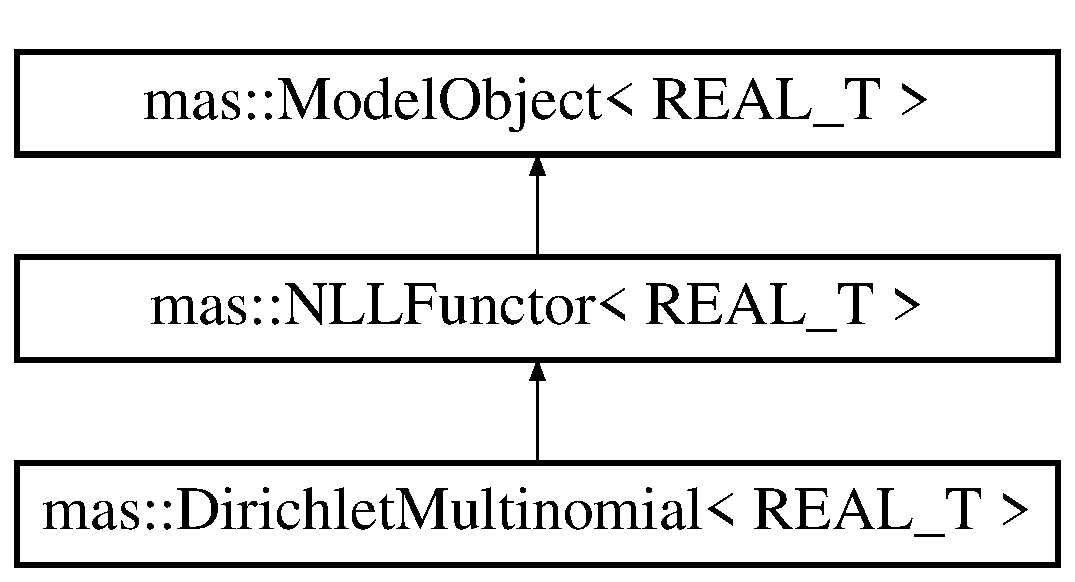
\includegraphics[height=3.000000cm]{structmas_1_1_dirichlet_multinomial}
\end{center}
\end{figure}
\subsection*{Public Types}
\begin{DoxyCompactItemize}
\item 
typedef \hyperlink{structmas_1_1_variable_trait}{Variable\-Trait}$<$ R\-E\-A\-L\-\_\-\-T $>$\\*
\-::\hyperlink{structmas_1_1_dirichlet_multinomial_a8e6915521c8c414ac50b545e6b77c4dd}{variable} \hyperlink{structmas_1_1_dirichlet_multinomial_a8e6915521c8c414ac50b545e6b77c4dd}{variable}
\end{DoxyCompactItemize}
\subsection*{Public Member Functions}
\begin{DoxyCompactItemize}
\item 
\hyperlink{structmas_1_1_dirichlet_multinomial_ac61d68fab90c2403c5def6943df1273c}{Dirichlet\-Multinomial} ()
\item 
\hyperlink{structmas_1_1_dirichlet_multinomial_ae9f8e90ada24b8179a2f45392c854375}{Dirichlet\-Multinomial} (size\-\_\-t \hyperlink{structmas_1_1_n_l_l_functor_ac76e5d7e0808486b42ffdaea952dd19f}{years}, size\-\_\-t \hyperlink{structmas_1_1_n_l_l_functor_ac59c36239b1817b5bb357bf90dc4802d}{seasons}, size\-\_\-t \hyperlink{structmas_1_1_n_l_l_functor_aa70e461c812bff95770cda5dbb79b6b9}{ages})
\item 
virtual \hyperlink{structmas_1_1_dirichlet_multinomial_a8e6915521c8c414ac50b545e6b77c4dd}{variable} \hyperlink{structmas_1_1_dirichlet_multinomial_ab65ba0749c9c746694ab4994e85e0a66}{Evaluate} (const std\-::shared\-\_\-ptr$<$ \hyperlink{structmas_1_1_data_object}{Data\-Object}$<$ R\-E\-A\-L\-\_\-\-T $>$ $>$ \&observed, const std\-::vector$<$ \hyperlink{structmas_1_1_dirichlet_multinomial_a8e6915521c8c414ac50b545e6b77c4dd}{variable} $>$ \&predicted, size\-\_\-t N)
\item 
virtual std\-::string \hyperlink{structmas_1_1_dirichlet_multinomial_a92d0abed181db2f54d7d44ac7cb4fa27}{To\-String} ()
\end{DoxyCompactItemize}
\subsection*{Public Attributes}
\begin{DoxyCompactItemize}
\item 
\hyperlink{structmas_1_1_dirichlet_multinomial_a8e6915521c8c414ac50b545e6b77c4dd}{variable} \hyperlink{structmas_1_1_dirichlet_multinomial_ac3ca50f28dcc152d0dc3d28866bb0e3e}{beta} = static\-\_\-cast$<$R\-E\-A\-L\-\_\-\-T$>$ (0.\-5)
\end{DoxyCompactItemize}


\subsection{Detailed Description}
\subsubsection*{template$<$typename R\-E\-A\-L\-\_\-\-T$>$struct mas\-::\-Dirichlet\-Multinomial$<$ R\-E\-A\-L\-\_\-\-T $>$}



Definition at line 155 of file N\-L\-L\-Components.\-hpp.



\subsection{Member Typedef Documentation}
\hypertarget{structmas_1_1_dirichlet_multinomial_a8e6915521c8c414ac50b545e6b77c4dd}{\index{mas\-::\-Dirichlet\-Multinomial@{mas\-::\-Dirichlet\-Multinomial}!variable@{variable}}
\index{variable@{variable}!mas::DirichletMultinomial@{mas\-::\-Dirichlet\-Multinomial}}
\subsubsection[{variable}]{\setlength{\rightskip}{0pt plus 5cm}template$<$typename R\-E\-A\-L\-\_\-\-T $>$ typedef {\bf Variable\-Trait}$<$R\-E\-A\-L\-\_\-\-T$>$\-::{\bf variable} {\bf mas\-::\-Dirichlet\-Multinomial}$<$ R\-E\-A\-L\-\_\-\-T $>$\-::{\bf variable}}}\label{structmas_1_1_dirichlet_multinomial_a8e6915521c8c414ac50b545e6b77c4dd}


Definition at line 156 of file N\-L\-L\-Components.\-hpp.



\subsection{Constructor \& Destructor Documentation}
\hypertarget{structmas_1_1_dirichlet_multinomial_ac61d68fab90c2403c5def6943df1273c}{\index{mas\-::\-Dirichlet\-Multinomial@{mas\-::\-Dirichlet\-Multinomial}!Dirichlet\-Multinomial@{Dirichlet\-Multinomial}}
\index{Dirichlet\-Multinomial@{Dirichlet\-Multinomial}!mas::DirichletMultinomial@{mas\-::\-Dirichlet\-Multinomial}}
\subsubsection[{Dirichlet\-Multinomial}]{\setlength{\rightskip}{0pt plus 5cm}template$<$typename R\-E\-A\-L\-\_\-\-T $>$ {\bf mas\-::\-Dirichlet\-Multinomial}$<$ R\-E\-A\-L\-\_\-\-T $>$\-::{\bf Dirichlet\-Multinomial} (
\begin{DoxyParamCaption}
{}
\end{DoxyParamCaption}
)\hspace{0.3cm}{\ttfamily [inline]}}}\label{structmas_1_1_dirichlet_multinomial_ac61d68fab90c2403c5def6943df1273c}


Definition at line 159 of file N\-L\-L\-Components.\-hpp.

\hypertarget{structmas_1_1_dirichlet_multinomial_ae9f8e90ada24b8179a2f45392c854375}{\index{mas\-::\-Dirichlet\-Multinomial@{mas\-::\-Dirichlet\-Multinomial}!Dirichlet\-Multinomial@{Dirichlet\-Multinomial}}
\index{Dirichlet\-Multinomial@{Dirichlet\-Multinomial}!mas::DirichletMultinomial@{mas\-::\-Dirichlet\-Multinomial}}
\subsubsection[{Dirichlet\-Multinomial}]{\setlength{\rightskip}{0pt plus 5cm}template$<$typename R\-E\-A\-L\-\_\-\-T $>$ {\bf mas\-::\-Dirichlet\-Multinomial}$<$ R\-E\-A\-L\-\_\-\-T $>$\-::{\bf Dirichlet\-Multinomial} (
\begin{DoxyParamCaption}
\item[{size\-\_\-t}]{years, }
\item[{size\-\_\-t}]{seasons, }
\item[{size\-\_\-t}]{ages}
\end{DoxyParamCaption}
)\hspace{0.3cm}{\ttfamily [inline]}}}\label{structmas_1_1_dirichlet_multinomial_ae9f8e90ada24b8179a2f45392c854375}


Definition at line 162 of file N\-L\-L\-Components.\-hpp.



\subsection{Member Function Documentation}
\hypertarget{structmas_1_1_dirichlet_multinomial_ab65ba0749c9c746694ab4994e85e0a66}{\index{mas\-::\-Dirichlet\-Multinomial@{mas\-::\-Dirichlet\-Multinomial}!Evaluate@{Evaluate}}
\index{Evaluate@{Evaluate}!mas::DirichletMultinomial@{mas\-::\-Dirichlet\-Multinomial}}
\subsubsection[{Evaluate}]{\setlength{\rightskip}{0pt plus 5cm}template$<$typename R\-E\-A\-L\-\_\-\-T $>$ virtual {\bf variable} {\bf mas\-::\-Dirichlet\-Multinomial}$<$ R\-E\-A\-L\-\_\-\-T $>$\-::Evaluate (
\begin{DoxyParamCaption}
\item[{const std\-::shared\-\_\-ptr$<$ {\bf Data\-Object}$<$ R\-E\-A\-L\-\_\-\-T $>$ $>$ \&}]{observed, }
\item[{const std\-::vector$<$ {\bf variable} $>$ \&}]{predicted, }
\item[{size\-\_\-t}]{N}
\end{DoxyParamCaption}
)\hspace{0.3cm}{\ttfamily [inline]}, {\ttfamily [virtual]}}}\label{structmas_1_1_dirichlet_multinomial_ab65ba0749c9c746694ab4994e85e0a66}


Implements \hyperlink{structmas_1_1_n_l_l_functor_a463977400e35ad46ef60c334d452cd6c}{mas\-::\-N\-L\-L\-Functor$<$ R\-E\-A\-L\-\_\-\-T $>$}.



Definition at line 166 of file N\-L\-L\-Components.\-hpp.

\hypertarget{structmas_1_1_dirichlet_multinomial_a92d0abed181db2f54d7d44ac7cb4fa27}{\index{mas\-::\-Dirichlet\-Multinomial@{mas\-::\-Dirichlet\-Multinomial}!To\-String@{To\-String}}
\index{To\-String@{To\-String}!mas::DirichletMultinomial@{mas\-::\-Dirichlet\-Multinomial}}
\subsubsection[{To\-String}]{\setlength{\rightskip}{0pt plus 5cm}template$<$typename R\-E\-A\-L\-\_\-\-T $>$ virtual std\-::string {\bf mas\-::\-Dirichlet\-Multinomial}$<$ R\-E\-A\-L\-\_\-\-T $>$\-::To\-String (
\begin{DoxyParamCaption}
{}
\end{DoxyParamCaption}
)\hspace{0.3cm}{\ttfamily [inline]}, {\ttfamily [virtual]}}}\label{structmas_1_1_dirichlet_multinomial_a92d0abed181db2f54d7d44ac7cb4fa27}


Reimplemented from \hyperlink{structmas_1_1_n_l_l_functor_accd55442e1e88b423471b67c40860197}{mas\-::\-N\-L\-L\-Functor$<$ R\-E\-A\-L\-\_\-\-T $>$}.



Definition at line 207 of file N\-L\-L\-Components.\-hpp.



\subsection{Member Data Documentation}
\hypertarget{structmas_1_1_dirichlet_multinomial_ac3ca50f28dcc152d0dc3d28866bb0e3e}{\index{mas\-::\-Dirichlet\-Multinomial@{mas\-::\-Dirichlet\-Multinomial}!beta@{beta}}
\index{beta@{beta}!mas::DirichletMultinomial@{mas\-::\-Dirichlet\-Multinomial}}
\subsubsection[{beta}]{\setlength{\rightskip}{0pt plus 5cm}template$<$typename R\-E\-A\-L\-\_\-\-T $>$ {\bf variable} {\bf mas\-::\-Dirichlet\-Multinomial}$<$ R\-E\-A\-L\-\_\-\-T $>$\-::beta = static\-\_\-cast$<$R\-E\-A\-L\-\_\-\-T$>$ (0.\-5)}}\label{structmas_1_1_dirichlet_multinomial_ac3ca50f28dcc152d0dc3d28866bb0e3e}


Definition at line 157 of file N\-L\-L\-Components.\-hpp.



The documentation for this struct was generated from the following file\-:\begin{DoxyCompactItemize}
\item 
/home/oppy/\-Net\-Beans\-Projects/mas/\hyperlink{_n_l_l_components_8hpp}{N\-L\-L\-Components.\-hpp}\end{DoxyCompactItemize}

\hypertarget{structmas_1_1_dirichlet_multinomial_robust}{\section{mas\-:\-:Dirichlet\-Multinomial\-Robust$<$ R\-E\-A\-L\-\_\-\-T $>$ Struct Template Reference}
\label{structmas_1_1_dirichlet_multinomial_robust}\index{mas\-::\-Dirichlet\-Multinomial\-Robust$<$ R\-E\-A\-L\-\_\-\-T $>$@{mas\-::\-Dirichlet\-Multinomial\-Robust$<$ R\-E\-A\-L\-\_\-\-T $>$}}
}


{\ttfamily \#include $<$N\-L\-L\-Components.\-hpp$>$}

Inheritance diagram for mas\-:\-:Dirichlet\-Multinomial\-Robust$<$ R\-E\-A\-L\-\_\-\-T $>$\-:\begin{figure}[H]
\begin{center}
\leavevmode
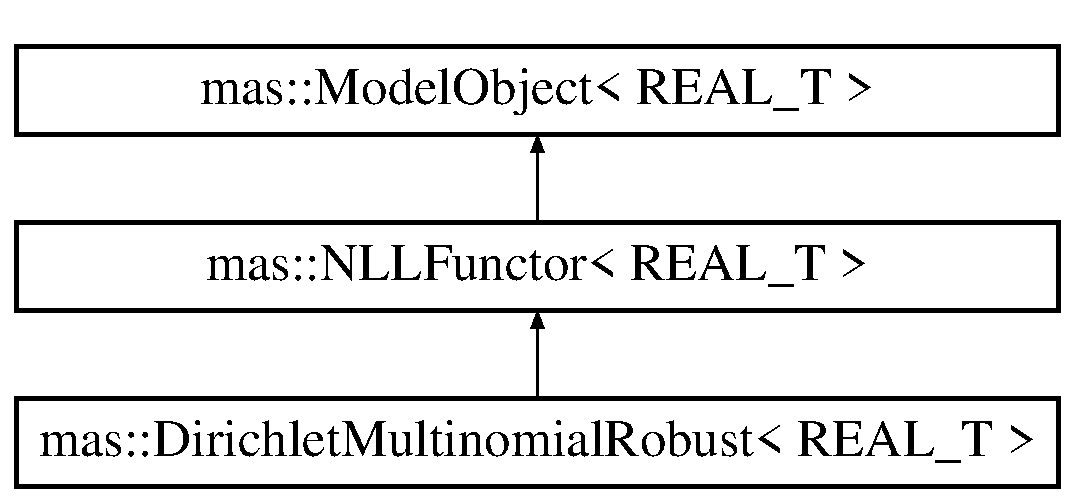
\includegraphics[height=3.000000cm]{structmas_1_1_dirichlet_multinomial_robust}
\end{center}
\end{figure}
\subsection*{Public Types}
\begin{DoxyCompactItemize}
\item 
typedef \hyperlink{structmas_1_1_variable_trait}{Variable\-Trait}$<$ R\-E\-A\-L\-\_\-\-T $>$\\*
\-::\hyperlink{structmas_1_1_dirichlet_multinomial_robust_ae46add67af1698359eaf6317847f42f1}{variable} \hyperlink{structmas_1_1_dirichlet_multinomial_robust_ae46add67af1698359eaf6317847f42f1}{variable}
\end{DoxyCompactItemize}
\subsection*{Public Member Functions}
\begin{DoxyCompactItemize}
\item 
\hyperlink{structmas_1_1_dirichlet_multinomial_robust_a9bda6773230596f595c6102350b6dc5b}{Dirichlet\-Multinomial\-Robust} ()
\item 
\hyperlink{structmas_1_1_dirichlet_multinomial_robust_a45404473a44ea179c9d01fd8d75c56a8}{Dirichlet\-Multinomial\-Robust} (size\-\_\-t \hyperlink{structmas_1_1_n_l_l_functor_ac76e5d7e0808486b42ffdaea952dd19f}{years}, size\-\_\-t \hyperlink{structmas_1_1_n_l_l_functor_ac59c36239b1817b5bb357bf90dc4802d}{seasons}, size\-\_\-t \hyperlink{structmas_1_1_n_l_l_functor_aa70e461c812bff95770cda5dbb79b6b9}{ages})
\item 
virtual \hyperlink{structmas_1_1_dirichlet_multinomial_robust_ae46add67af1698359eaf6317847f42f1}{variable} \hyperlink{structmas_1_1_dirichlet_multinomial_robust_accc5e689e123bac3c30a8f54240f63d7}{Evaluate} (const std\-::shared\-\_\-ptr$<$ \hyperlink{structmas_1_1_data_object}{Data\-Object}$<$ R\-E\-A\-L\-\_\-\-T $>$ $>$ \&observed, const std\-::vector$<$ \hyperlink{structmas_1_1_dirichlet_multinomial_robust_ae46add67af1698359eaf6317847f42f1}{variable} $>$ \&predicted, size\-\_\-t N)
\item 
virtual std\-::string \hyperlink{structmas_1_1_dirichlet_multinomial_robust_a25f3b78a3072162c8e1fce217a599a14}{To\-String} ()
\end{DoxyCompactItemize}
\subsection*{Public Attributes}
\begin{DoxyCompactItemize}
\item 
\hyperlink{structmas_1_1_dirichlet_multinomial_robust_ae46add67af1698359eaf6317847f42f1}{variable} \hyperlink{structmas_1_1_dirichlet_multinomial_robust_a5b440cc461e06eb9abbc824fbf9dacff}{beta} = static\-\_\-cast$<$R\-E\-A\-L\-\_\-\-T$>$ (0.\-5)
\item 
R\-E\-A\-L\-\_\-\-T \hyperlink{structmas_1_1_dirichlet_multinomial_robust_a7f16f0414a3ad99ca01df8e9df5a0785}{epsilon} = static\-\_\-cast$<$R\-E\-A\-L\-\_\-\-T$>$ (1e-\/8)
\end{DoxyCompactItemize}


\subsection{Detailed Description}
\subsubsection*{template$<$typename R\-E\-A\-L\-\_\-\-T$>$struct mas\-::\-Dirichlet\-Multinomial\-Robust$<$ R\-E\-A\-L\-\_\-\-T $>$}



Definition at line 213 of file N\-L\-L\-Components.\-hpp.



\subsection{Member Typedef Documentation}
\hypertarget{structmas_1_1_dirichlet_multinomial_robust_ae46add67af1698359eaf6317847f42f1}{\index{mas\-::\-Dirichlet\-Multinomial\-Robust@{mas\-::\-Dirichlet\-Multinomial\-Robust}!variable@{variable}}
\index{variable@{variable}!mas::DirichletMultinomialRobust@{mas\-::\-Dirichlet\-Multinomial\-Robust}}
\subsubsection[{variable}]{\setlength{\rightskip}{0pt plus 5cm}template$<$typename R\-E\-A\-L\-\_\-\-T $>$ typedef {\bf Variable\-Trait}$<$R\-E\-A\-L\-\_\-\-T$>$\-::{\bf variable} {\bf mas\-::\-Dirichlet\-Multinomial\-Robust}$<$ R\-E\-A\-L\-\_\-\-T $>$\-::{\bf variable}}}\label{structmas_1_1_dirichlet_multinomial_robust_ae46add67af1698359eaf6317847f42f1}


Definition at line 214 of file N\-L\-L\-Components.\-hpp.



\subsection{Constructor \& Destructor Documentation}
\hypertarget{structmas_1_1_dirichlet_multinomial_robust_a9bda6773230596f595c6102350b6dc5b}{\index{mas\-::\-Dirichlet\-Multinomial\-Robust@{mas\-::\-Dirichlet\-Multinomial\-Robust}!Dirichlet\-Multinomial\-Robust@{Dirichlet\-Multinomial\-Robust}}
\index{Dirichlet\-Multinomial\-Robust@{Dirichlet\-Multinomial\-Robust}!mas::DirichletMultinomialRobust@{mas\-::\-Dirichlet\-Multinomial\-Robust}}
\subsubsection[{Dirichlet\-Multinomial\-Robust}]{\setlength{\rightskip}{0pt plus 5cm}template$<$typename R\-E\-A\-L\-\_\-\-T $>$ {\bf mas\-::\-Dirichlet\-Multinomial\-Robust}$<$ R\-E\-A\-L\-\_\-\-T $>$\-::{\bf Dirichlet\-Multinomial\-Robust} (
\begin{DoxyParamCaption}
{}
\end{DoxyParamCaption}
)\hspace{0.3cm}{\ttfamily [inline]}}}\label{structmas_1_1_dirichlet_multinomial_robust_a9bda6773230596f595c6102350b6dc5b}


Definition at line 218 of file N\-L\-L\-Components.\-hpp.

\hypertarget{structmas_1_1_dirichlet_multinomial_robust_a45404473a44ea179c9d01fd8d75c56a8}{\index{mas\-::\-Dirichlet\-Multinomial\-Robust@{mas\-::\-Dirichlet\-Multinomial\-Robust}!Dirichlet\-Multinomial\-Robust@{Dirichlet\-Multinomial\-Robust}}
\index{Dirichlet\-Multinomial\-Robust@{Dirichlet\-Multinomial\-Robust}!mas::DirichletMultinomialRobust@{mas\-::\-Dirichlet\-Multinomial\-Robust}}
\subsubsection[{Dirichlet\-Multinomial\-Robust}]{\setlength{\rightskip}{0pt plus 5cm}template$<$typename R\-E\-A\-L\-\_\-\-T $>$ {\bf mas\-::\-Dirichlet\-Multinomial\-Robust}$<$ R\-E\-A\-L\-\_\-\-T $>$\-::{\bf Dirichlet\-Multinomial\-Robust} (
\begin{DoxyParamCaption}
\item[{size\-\_\-t}]{years, }
\item[{size\-\_\-t}]{seasons, }
\item[{size\-\_\-t}]{ages}
\end{DoxyParamCaption}
)\hspace{0.3cm}{\ttfamily [inline]}}}\label{structmas_1_1_dirichlet_multinomial_robust_a45404473a44ea179c9d01fd8d75c56a8}


Definition at line 221 of file N\-L\-L\-Components.\-hpp.



\subsection{Member Function Documentation}
\hypertarget{structmas_1_1_dirichlet_multinomial_robust_accc5e689e123bac3c30a8f54240f63d7}{\index{mas\-::\-Dirichlet\-Multinomial\-Robust@{mas\-::\-Dirichlet\-Multinomial\-Robust}!Evaluate@{Evaluate}}
\index{Evaluate@{Evaluate}!mas::DirichletMultinomialRobust@{mas\-::\-Dirichlet\-Multinomial\-Robust}}
\subsubsection[{Evaluate}]{\setlength{\rightskip}{0pt plus 5cm}template$<$typename R\-E\-A\-L\-\_\-\-T $>$ virtual {\bf variable} {\bf mas\-::\-Dirichlet\-Multinomial\-Robust}$<$ R\-E\-A\-L\-\_\-\-T $>$\-::Evaluate (
\begin{DoxyParamCaption}
\item[{const std\-::shared\-\_\-ptr$<$ {\bf Data\-Object}$<$ R\-E\-A\-L\-\_\-\-T $>$ $>$ \&}]{observed, }
\item[{const std\-::vector$<$ {\bf variable} $>$ \&}]{predicted, }
\item[{size\-\_\-t}]{N}
\end{DoxyParamCaption}
)\hspace{0.3cm}{\ttfamily [inline]}, {\ttfamily [virtual]}}}\label{structmas_1_1_dirichlet_multinomial_robust_accc5e689e123bac3c30a8f54240f63d7}


Implements \hyperlink{structmas_1_1_n_l_l_functor_a463977400e35ad46ef60c334d452cd6c}{mas\-::\-N\-L\-L\-Functor$<$ R\-E\-A\-L\-\_\-\-T $>$}.



Definition at line 225 of file N\-L\-L\-Components.\-hpp.

\hypertarget{structmas_1_1_dirichlet_multinomial_robust_a25f3b78a3072162c8e1fce217a599a14}{\index{mas\-::\-Dirichlet\-Multinomial\-Robust@{mas\-::\-Dirichlet\-Multinomial\-Robust}!To\-String@{To\-String}}
\index{To\-String@{To\-String}!mas::DirichletMultinomialRobust@{mas\-::\-Dirichlet\-Multinomial\-Robust}}
\subsubsection[{To\-String}]{\setlength{\rightskip}{0pt plus 5cm}template$<$typename R\-E\-A\-L\-\_\-\-T $>$ virtual std\-::string {\bf mas\-::\-Dirichlet\-Multinomial\-Robust}$<$ R\-E\-A\-L\-\_\-\-T $>$\-::To\-String (
\begin{DoxyParamCaption}
{}
\end{DoxyParamCaption}
)\hspace{0.3cm}{\ttfamily [inline]}, {\ttfamily [virtual]}}}\label{structmas_1_1_dirichlet_multinomial_robust_a25f3b78a3072162c8e1fce217a599a14}


Reimplemented from \hyperlink{structmas_1_1_n_l_l_functor_accd55442e1e88b423471b67c40860197}{mas\-::\-N\-L\-L\-Functor$<$ R\-E\-A\-L\-\_\-\-T $>$}.



Definition at line 273 of file N\-L\-L\-Components.\-hpp.



\subsection{Member Data Documentation}
\hypertarget{structmas_1_1_dirichlet_multinomial_robust_a5b440cc461e06eb9abbc824fbf9dacff}{\index{mas\-::\-Dirichlet\-Multinomial\-Robust@{mas\-::\-Dirichlet\-Multinomial\-Robust}!beta@{beta}}
\index{beta@{beta}!mas::DirichletMultinomialRobust@{mas\-::\-Dirichlet\-Multinomial\-Robust}}
\subsubsection[{beta}]{\setlength{\rightskip}{0pt plus 5cm}template$<$typename R\-E\-A\-L\-\_\-\-T $>$ {\bf variable} {\bf mas\-::\-Dirichlet\-Multinomial\-Robust}$<$ R\-E\-A\-L\-\_\-\-T $>$\-::beta = static\-\_\-cast$<$R\-E\-A\-L\-\_\-\-T$>$ (0.\-5)}}\label{structmas_1_1_dirichlet_multinomial_robust_a5b440cc461e06eb9abbc824fbf9dacff}


Definition at line 215 of file N\-L\-L\-Components.\-hpp.

\hypertarget{structmas_1_1_dirichlet_multinomial_robust_a7f16f0414a3ad99ca01df8e9df5a0785}{\index{mas\-::\-Dirichlet\-Multinomial\-Robust@{mas\-::\-Dirichlet\-Multinomial\-Robust}!epsilon@{epsilon}}
\index{epsilon@{epsilon}!mas::DirichletMultinomialRobust@{mas\-::\-Dirichlet\-Multinomial\-Robust}}
\subsubsection[{epsilon}]{\setlength{\rightskip}{0pt plus 5cm}template$<$typename R\-E\-A\-L\-\_\-\-T $>$ R\-E\-A\-L\-\_\-\-T {\bf mas\-::\-Dirichlet\-Multinomial\-Robust}$<$ R\-E\-A\-L\-\_\-\-T $>$\-::epsilon = static\-\_\-cast$<$R\-E\-A\-L\-\_\-\-T$>$ (1e-\/8)}}\label{structmas_1_1_dirichlet_multinomial_robust_a7f16f0414a3ad99ca01df8e9df5a0785}


Definition at line 216 of file N\-L\-L\-Components.\-hpp.



The documentation for this struct was generated from the following file\-:\begin{DoxyCompactItemize}
\item 
/home/oppy/\-Net\-Beans\-Projects/mas/\hyperlink{_n_l_l_components_8hpp}{N\-L\-L\-Components.\-hpp}\end{DoxyCompactItemize}

\hypertarget{structmas_1_1_double_logistic_fec}{\section{mas\-:\-:Double\-Logistic\-Fec$<$ R\-E\-A\-L\-\_\-\-T $>$ Struct Template Reference}
\label{structmas_1_1_double_logistic_fec}\index{mas\-::\-Double\-Logistic\-Fec$<$ R\-E\-A\-L\-\_\-\-T $>$@{mas\-::\-Double\-Logistic\-Fec$<$ R\-E\-A\-L\-\_\-\-T $>$}}
}


{\ttfamily \#include $<$Fecundity.\-hpp$>$}

Inheritance diagram for mas\-:\-:Double\-Logistic\-Fec$<$ R\-E\-A\-L\-\_\-\-T $>$\-:\begin{figure}[H]
\begin{center}
\leavevmode
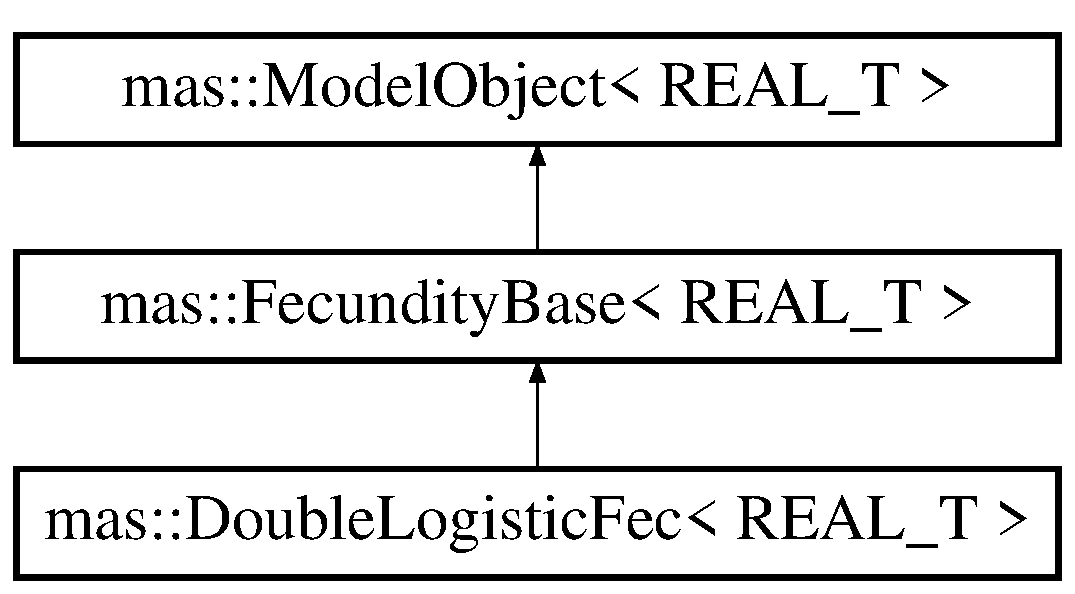
\includegraphics[height=3.000000cm]{structmas_1_1_double_logistic_fec}
\end{center}
\end{figure}
\subsection*{Public Types}
\begin{DoxyCompactItemize}
\item 
typedef \hyperlink{structmas_1_1_variable_trait}{Variable\-Trait}$<$ R\-E\-A\-L\-\_\-\-T $>$\\*
\-::\hyperlink{structmas_1_1_double_logistic_fec_abfb3cdee2e273df6dbffdb71bba6ab9c}{variable} \hyperlink{structmas_1_1_double_logistic_fec_abfb3cdee2e273df6dbffdb71bba6ab9c}{variable}
\end{DoxyCompactItemize}
\subsection*{Public Member Functions}
\begin{DoxyCompactItemize}
\item 
virtual const \hyperlink{structmas_1_1_double_logistic_fec_abfb3cdee2e273df6dbffdb71bba6ab9c}{variable} \hyperlink{structmas_1_1_double_logistic_fec_a732cf8310636c612ed4a6cf78079e03b}{Evaluate} (const int \&sex, const \hyperlink{structmas_1_1_double_logistic_fec_abfb3cdee2e273df6dbffdb71bba6ab9c}{variable} \&age)
\item 
virtual const std\-::string \hyperlink{structmas_1_1_double_logistic_fec_a08517ef4ed14c1dc4e6fdce9baafbae0}{Name} ()
\end{DoxyCompactItemize}
\subsection*{Public Attributes}
\begin{DoxyCompactItemize}
\item 
\hyperlink{structmas_1_1_double_logistic_fec_abfb3cdee2e273df6dbffdb71bba6ab9c}{variable} \hyperlink{structmas_1_1_double_logistic_fec_a842802b2a752f90e7573f64c39f804b1}{alpha\-\_\-asc}
\item 
\hyperlink{structmas_1_1_double_logistic_fec_abfb3cdee2e273df6dbffdb71bba6ab9c}{variable} \hyperlink{structmas_1_1_double_logistic_fec_a60a24a306e30464e33b1884fc53a1435}{beta\-\_\-asc}
\item 
\hyperlink{structmas_1_1_double_logistic_fec_abfb3cdee2e273df6dbffdb71bba6ab9c}{variable} \hyperlink{structmas_1_1_double_logistic_fec_a62ce4cb22c93f6a2fac67c7ab129749d}{alpha\-\_\-desc}
\item 
\hyperlink{structmas_1_1_double_logistic_fec_abfb3cdee2e273df6dbffdb71bba6ab9c}{variable} \hyperlink{structmas_1_1_double_logistic_fec_a34f906fdd181ef464af015fa8b95432d}{beta\-\_\-desc}
\end{DoxyCompactItemize}


\subsection{Detailed Description}
\subsubsection*{template$<$typename R\-E\-A\-L\-\_\-\-T$>$struct mas\-::\-Double\-Logistic\-Fec$<$ R\-E\-A\-L\-\_\-\-T $>$}



Definition at line 78 of file Fecundity.\-hpp.



\subsection{Member Typedef Documentation}
\hypertarget{structmas_1_1_double_logistic_fec_abfb3cdee2e273df6dbffdb71bba6ab9c}{\index{mas\-::\-Double\-Logistic\-Fec@{mas\-::\-Double\-Logistic\-Fec}!variable@{variable}}
\index{variable@{variable}!mas::DoubleLogisticFec@{mas\-::\-Double\-Logistic\-Fec}}
\subsubsection[{variable}]{\setlength{\rightskip}{0pt plus 5cm}template$<$typename R\-E\-A\-L\-\_\-\-T $>$ typedef {\bf Variable\-Trait}$<$R\-E\-A\-L\-\_\-\-T$>$\-::{\bf variable} {\bf mas\-::\-Double\-Logistic\-Fec}$<$ R\-E\-A\-L\-\_\-\-T $>$\-::{\bf variable}}}\label{structmas_1_1_double_logistic_fec_abfb3cdee2e273df6dbffdb71bba6ab9c}


Definition at line 79 of file Fecundity.\-hpp.



\subsection{Member Function Documentation}
\hypertarget{structmas_1_1_double_logistic_fec_a732cf8310636c612ed4a6cf78079e03b}{\index{mas\-::\-Double\-Logistic\-Fec@{mas\-::\-Double\-Logistic\-Fec}!Evaluate@{Evaluate}}
\index{Evaluate@{Evaluate}!mas::DoubleLogisticFec@{mas\-::\-Double\-Logistic\-Fec}}
\subsubsection[{Evaluate}]{\setlength{\rightskip}{0pt plus 5cm}template$<$typename R\-E\-A\-L\-\_\-\-T $>$ virtual const {\bf variable} {\bf mas\-::\-Double\-Logistic\-Fec}$<$ R\-E\-A\-L\-\_\-\-T $>$\-::Evaluate (
\begin{DoxyParamCaption}
\item[{const int \&}]{sex, }
\item[{const {\bf variable} \&}]{age}
\end{DoxyParamCaption}
)\hspace{0.3cm}{\ttfamily [inline]}, {\ttfamily [virtual]}}}\label{structmas_1_1_double_logistic_fec_a732cf8310636c612ed4a6cf78079e03b}
Age based double logistic maturity


\begin{DoxyParams}{Parameters}
{\em sex} & \\
\hline
{\em age} & \\
\hline
\end{DoxyParams}
\begin{DoxyReturn}{Returns}
fraction\-\_\-mature 
\end{DoxyReturn}


Implements \hyperlink{structmas_1_1_fecundity_base_a44573d4082a65920010d9d20ed2d8e14}{mas\-::\-Fecundity\-Base$<$ R\-E\-A\-L\-\_\-\-T $>$}.



Definition at line 92 of file Fecundity.\-hpp.

\hypertarget{structmas_1_1_double_logistic_fec_a08517ef4ed14c1dc4e6fdce9baafbae0}{\index{mas\-::\-Double\-Logistic\-Fec@{mas\-::\-Double\-Logistic\-Fec}!Name@{Name}}
\index{Name@{Name}!mas::DoubleLogisticFec@{mas\-::\-Double\-Logistic\-Fec}}
\subsubsection[{Name}]{\setlength{\rightskip}{0pt plus 5cm}template$<$typename R\-E\-A\-L\-\_\-\-T $>$ virtual const std\-::string {\bf mas\-::\-Double\-Logistic\-Fec}$<$ R\-E\-A\-L\-\_\-\-T $>$\-::Name (
\begin{DoxyParamCaption}
{}
\end{DoxyParamCaption}
)\hspace{0.3cm}{\ttfamily [inline]}, {\ttfamily [virtual]}}}\label{structmas_1_1_double_logistic_fec_a08517ef4ed14c1dc4e6fdce9baafbae0}


Reimplemented from \hyperlink{structmas_1_1_fecundity_base_a5a0ca3b02791910dd012a30f1c2bf2a8}{mas\-::\-Fecundity\-Base$<$ R\-E\-A\-L\-\_\-\-T $>$}.



Definition at line 101 of file Fecundity.\-hpp.



\subsection{Member Data Documentation}
\hypertarget{structmas_1_1_double_logistic_fec_a842802b2a752f90e7573f64c39f804b1}{\index{mas\-::\-Double\-Logistic\-Fec@{mas\-::\-Double\-Logistic\-Fec}!alpha\-\_\-asc@{alpha\-\_\-asc}}
\index{alpha\-\_\-asc@{alpha\-\_\-asc}!mas::DoubleLogisticFec@{mas\-::\-Double\-Logistic\-Fec}}
\subsubsection[{alpha\-\_\-asc}]{\setlength{\rightskip}{0pt plus 5cm}template$<$typename R\-E\-A\-L\-\_\-\-T $>$ {\bf variable} {\bf mas\-::\-Double\-Logistic\-Fec}$<$ R\-E\-A\-L\-\_\-\-T $>$\-::alpha\-\_\-asc}}\label{structmas_1_1_double_logistic_fec_a842802b2a752f90e7573f64c39f804b1}


Definition at line 80 of file Fecundity.\-hpp.

\hypertarget{structmas_1_1_double_logistic_fec_a62ce4cb22c93f6a2fac67c7ab129749d}{\index{mas\-::\-Double\-Logistic\-Fec@{mas\-::\-Double\-Logistic\-Fec}!alpha\-\_\-desc@{alpha\-\_\-desc}}
\index{alpha\-\_\-desc@{alpha\-\_\-desc}!mas::DoubleLogisticFec@{mas\-::\-Double\-Logistic\-Fec}}
\subsubsection[{alpha\-\_\-desc}]{\setlength{\rightskip}{0pt plus 5cm}template$<$typename R\-E\-A\-L\-\_\-\-T $>$ {\bf variable} {\bf mas\-::\-Double\-Logistic\-Fec}$<$ R\-E\-A\-L\-\_\-\-T $>$\-::alpha\-\_\-desc}}\label{structmas_1_1_double_logistic_fec_a62ce4cb22c93f6a2fac67c7ab129749d}


Definition at line 82 of file Fecundity.\-hpp.

\hypertarget{structmas_1_1_double_logistic_fec_a60a24a306e30464e33b1884fc53a1435}{\index{mas\-::\-Double\-Logistic\-Fec@{mas\-::\-Double\-Logistic\-Fec}!beta\-\_\-asc@{beta\-\_\-asc}}
\index{beta\-\_\-asc@{beta\-\_\-asc}!mas::DoubleLogisticFec@{mas\-::\-Double\-Logistic\-Fec}}
\subsubsection[{beta\-\_\-asc}]{\setlength{\rightskip}{0pt plus 5cm}template$<$typename R\-E\-A\-L\-\_\-\-T $>$ {\bf variable} {\bf mas\-::\-Double\-Logistic\-Fec}$<$ R\-E\-A\-L\-\_\-\-T $>$\-::beta\-\_\-asc}}\label{structmas_1_1_double_logistic_fec_a60a24a306e30464e33b1884fc53a1435}


Definition at line 81 of file Fecundity.\-hpp.

\hypertarget{structmas_1_1_double_logistic_fec_a34f906fdd181ef464af015fa8b95432d}{\index{mas\-::\-Double\-Logistic\-Fec@{mas\-::\-Double\-Logistic\-Fec}!beta\-\_\-desc@{beta\-\_\-desc}}
\index{beta\-\_\-desc@{beta\-\_\-desc}!mas::DoubleLogisticFec@{mas\-::\-Double\-Logistic\-Fec}}
\subsubsection[{beta\-\_\-desc}]{\setlength{\rightskip}{0pt plus 5cm}template$<$typename R\-E\-A\-L\-\_\-\-T $>$ {\bf variable} {\bf mas\-::\-Double\-Logistic\-Fec}$<$ R\-E\-A\-L\-\_\-\-T $>$\-::beta\-\_\-desc}}\label{structmas_1_1_double_logistic_fec_a34f906fdd181ef464af015fa8b95432d}


Definition at line 83 of file Fecundity.\-hpp.



The documentation for this struct was generated from the following file\-:\begin{DoxyCompactItemize}
\item 
/home/oppy/\-Net\-Beans\-Projects/mas/\hyperlink{_fecundity_8hpp}{Fecundity.\-hpp}\end{DoxyCompactItemize}

\hypertarget{structmas_1_1_double_logistic_sel}{\section{mas\-:\-:Double\-Logistic\-Sel$<$ R\-E\-A\-L\-\_\-\-T $>$ Struct Template Reference}
\label{structmas_1_1_double_logistic_sel}\index{mas\-::\-Double\-Logistic\-Sel$<$ R\-E\-A\-L\-\_\-\-T $>$@{mas\-::\-Double\-Logistic\-Sel$<$ R\-E\-A\-L\-\_\-\-T $>$}}
}


{\ttfamily \#include $<$Selectivity.\-hpp$>$}

Inheritance diagram for mas\-:\-:Double\-Logistic\-Sel$<$ R\-E\-A\-L\-\_\-\-T $>$\-:\begin{figure}[H]
\begin{center}
\leavevmode
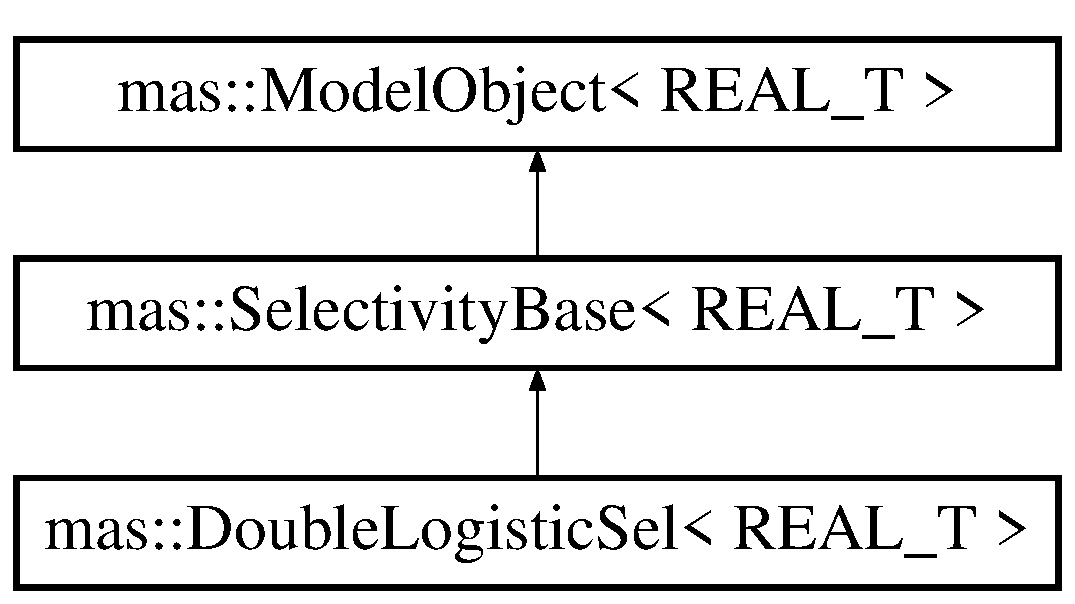
\includegraphics[height=3.000000cm]{structmas_1_1_double_logistic_sel}
\end{center}
\end{figure}
\subsection*{Public Types}
\begin{DoxyCompactItemize}
\item 
typedef \hyperlink{structmas_1_1_variable_trait}{Variable\-Trait}$<$ R\-E\-A\-L\-\_\-\-T $>$\\*
\-::\hyperlink{structmas_1_1_double_logistic_sel_aa9c8db47e992fdddb25f535eb0d6b343}{variable} \hyperlink{structmas_1_1_double_logistic_sel_aa9c8db47e992fdddb25f535eb0d6b343}{variable}
\end{DoxyCompactItemize}
\subsection*{Public Member Functions}
\begin{DoxyCompactItemize}
\item 
virtual const \hyperlink{structmas_1_1_double_logistic_sel_aa9c8db47e992fdddb25f535eb0d6b343}{variable} \hyperlink{structmas_1_1_double_logistic_sel_a90935c4bb22641c8e3f6e9e742c785ac}{Evaluate} (const \hyperlink{structmas_1_1_double_logistic_sel_aa9c8db47e992fdddb25f535eb0d6b343}{variable} \&a)
\item 
virtual const \hyperlink{structmas_1_1_double_logistic_sel_aa9c8db47e992fdddb25f535eb0d6b343}{variable} \hyperlink{structmas_1_1_double_logistic_sel_ae6c78421dea075fd43bdd30ab0d8fad5}{Evaluate} (const std\-::vector$<$ \hyperlink{structmas_1_1_double_logistic_sel_aa9c8db47e992fdddb25f535eb0d6b343}{variable} $>$ \&ages, size\-\_\-t index)
\item 
virtual const std\-::string \hyperlink{structmas_1_1_double_logistic_sel_af25cc89b1ae6e3b53774c59b8b440699}{To\-J\-S\-O\-N\-String} ()
\item 
virtual const std\-::string \hyperlink{structmas_1_1_double_logistic_sel_a1f71e8df42eb1d1b7b54df4e0427d05b}{Name} ()
\item 
virtual std\-::string \hyperlink{structmas_1_1_double_logistic_sel_ab91353c57277a40f04c505ce77332c65}{To\-String} ()
\end{DoxyCompactItemize}
\subsection*{Public Attributes}
\begin{DoxyCompactItemize}
\item 
\hyperlink{structmas_1_1_double_logistic_sel_aa9c8db47e992fdddb25f535eb0d6b343}{variable} \hyperlink{structmas_1_1_double_logistic_sel_a91765c136da3707bc8500ef4459b801e}{alpha\-\_\-asc}
\item 
\hyperlink{structmas_1_1_double_logistic_sel_aa9c8db47e992fdddb25f535eb0d6b343}{variable} \hyperlink{structmas_1_1_double_logistic_sel_ace010a06a23e4a9145c61c5d022167c6}{beta\-\_\-asc}
\item 
\hyperlink{structmas_1_1_double_logistic_sel_aa9c8db47e992fdddb25f535eb0d6b343}{variable} \hyperlink{structmas_1_1_double_logistic_sel_af9b785ac193b2d14ab923f5a04818abe}{alpha\-\_\-desc}
\item 
\hyperlink{structmas_1_1_double_logistic_sel_aa9c8db47e992fdddb25f535eb0d6b343}{variable} \hyperlink{structmas_1_1_double_logistic_sel_a565d907c1dbd00686a08d624c4b891ea}{beta\-\_\-desc}
\end{DoxyCompactItemize}


\subsection{Detailed Description}
\subsubsection*{template$<$typename R\-E\-A\-L\-\_\-\-T$>$struct mas\-::\-Double\-Logistic\-Sel$<$ R\-E\-A\-L\-\_\-\-T $>$}



Definition at line 99 of file Selectivity.\-hpp.



\subsection{Member Typedef Documentation}
\hypertarget{structmas_1_1_double_logistic_sel_aa9c8db47e992fdddb25f535eb0d6b343}{\index{mas\-::\-Double\-Logistic\-Sel@{mas\-::\-Double\-Logistic\-Sel}!variable@{variable}}
\index{variable@{variable}!mas::DoubleLogisticSel@{mas\-::\-Double\-Logistic\-Sel}}
\subsubsection[{variable}]{\setlength{\rightskip}{0pt plus 5cm}template$<$typename R\-E\-A\-L\-\_\-\-T $>$ typedef {\bf Variable\-Trait}$<$R\-E\-A\-L\-\_\-\-T$>$\-::{\bf variable} {\bf mas\-::\-Double\-Logistic\-Sel}$<$ R\-E\-A\-L\-\_\-\-T $>$\-::{\bf variable}}}\label{structmas_1_1_double_logistic_sel_aa9c8db47e992fdddb25f535eb0d6b343}


Definition at line 100 of file Selectivity.\-hpp.



\subsection{Member Function Documentation}
\hypertarget{structmas_1_1_double_logistic_sel_a90935c4bb22641c8e3f6e9e742c785ac}{\index{mas\-::\-Double\-Logistic\-Sel@{mas\-::\-Double\-Logistic\-Sel}!Evaluate@{Evaluate}}
\index{Evaluate@{Evaluate}!mas::DoubleLogisticSel@{mas\-::\-Double\-Logistic\-Sel}}
\subsubsection[{Evaluate}]{\setlength{\rightskip}{0pt plus 5cm}template$<$typename R\-E\-A\-L\-\_\-\-T $>$ virtual const {\bf variable} {\bf mas\-::\-Double\-Logistic\-Sel}$<$ R\-E\-A\-L\-\_\-\-T $>$\-::Evaluate (
\begin{DoxyParamCaption}
\item[{const {\bf variable} \&}]{a}
\end{DoxyParamCaption}
)\hspace{0.3cm}{\ttfamily [inline]}, {\ttfamily [virtual]}}}\label{structmas_1_1_double_logistic_sel_a90935c4bb22641c8e3f6e9e742c785ac}
Age based logistic selectivity 
\begin{DoxyParams}{Parameters}
{\em a} & -\/ age \\
\hline
\end{DoxyParams}
\begin{DoxyReturn}{Returns}

\end{DoxyReturn}


Implements \hyperlink{structmas_1_1_selectivity_base_a1c26fb2107d380ac4540271280031bf4}{mas\-::\-Selectivity\-Base$<$ R\-E\-A\-L\-\_\-\-T $>$}.



Definition at line 111 of file Selectivity.\-hpp.

\hypertarget{structmas_1_1_double_logistic_sel_ae6c78421dea075fd43bdd30ab0d8fad5}{\index{mas\-::\-Double\-Logistic\-Sel@{mas\-::\-Double\-Logistic\-Sel}!Evaluate@{Evaluate}}
\index{Evaluate@{Evaluate}!mas::DoubleLogisticSel@{mas\-::\-Double\-Logistic\-Sel}}
\subsubsection[{Evaluate}]{\setlength{\rightskip}{0pt plus 5cm}template$<$typename R\-E\-A\-L\-\_\-\-T $>$ virtual const {\bf variable} {\bf mas\-::\-Double\-Logistic\-Sel}$<$ R\-E\-A\-L\-\_\-\-T $>$\-::Evaluate (
\begin{DoxyParamCaption}
\item[{const std\-::vector$<$ {\bf variable} $>$ \&}]{ages, }
\item[{size\-\_\-t}]{index}
\end{DoxyParamCaption}
)\hspace{0.3cm}{\ttfamily [inline]}, {\ttfamily [virtual]}}}\label{structmas_1_1_double_logistic_sel_ae6c78421dea075fd43bdd30ab0d8fad5}


Implements \hyperlink{structmas_1_1_selectivity_base_a52058fc9fe373bcc6deebd43bfc3f402}{mas\-::\-Selectivity\-Base$<$ R\-E\-A\-L\-\_\-\-T $>$}.



Definition at line 120 of file Selectivity.\-hpp.

\hypertarget{structmas_1_1_double_logistic_sel_a1f71e8df42eb1d1b7b54df4e0427d05b}{\index{mas\-::\-Double\-Logistic\-Sel@{mas\-::\-Double\-Logistic\-Sel}!Name@{Name}}
\index{Name@{Name}!mas::DoubleLogisticSel@{mas\-::\-Double\-Logistic\-Sel}}
\subsubsection[{Name}]{\setlength{\rightskip}{0pt plus 5cm}template$<$typename R\-E\-A\-L\-\_\-\-T $>$ virtual const std\-::string {\bf mas\-::\-Double\-Logistic\-Sel}$<$ R\-E\-A\-L\-\_\-\-T $>$\-::Name (
\begin{DoxyParamCaption}
{}
\end{DoxyParamCaption}
)\hspace{0.3cm}{\ttfamily [inline]}, {\ttfamily [virtual]}}}\label{structmas_1_1_double_logistic_sel_a1f71e8df42eb1d1b7b54df4e0427d05b}


Reimplemented from \hyperlink{structmas_1_1_selectivity_base_ad14deefa4cddcc1c93ef17cc0a3e566a}{mas\-::\-Selectivity\-Base$<$ R\-E\-A\-L\-\_\-\-T $>$}.



Definition at line 144 of file Selectivity.\-hpp.

\hypertarget{structmas_1_1_double_logistic_sel_af25cc89b1ae6e3b53774c59b8b440699}{\index{mas\-::\-Double\-Logistic\-Sel@{mas\-::\-Double\-Logistic\-Sel}!To\-J\-S\-O\-N\-String@{To\-J\-S\-O\-N\-String}}
\index{To\-J\-S\-O\-N\-String@{To\-J\-S\-O\-N\-String}!mas::DoubleLogisticSel@{mas\-::\-Double\-Logistic\-Sel}}
\subsubsection[{To\-J\-S\-O\-N\-String}]{\setlength{\rightskip}{0pt plus 5cm}template$<$typename R\-E\-A\-L\-\_\-\-T $>$ virtual const std\-::string {\bf mas\-::\-Double\-Logistic\-Sel}$<$ R\-E\-A\-L\-\_\-\-T $>$\-::To\-J\-S\-O\-N\-String (
\begin{DoxyParamCaption}
{}
\end{DoxyParamCaption}
)\hspace{0.3cm}{\ttfamily [inline]}, {\ttfamily [virtual]}}}\label{structmas_1_1_double_logistic_sel_af25cc89b1ae6e3b53774c59b8b440699}


Reimplemented from \hyperlink{structmas_1_1_model_object_af40b3c89b11919fc5aea21dcf1cd027b}{mas\-::\-Model\-Object$<$ R\-E\-A\-L\-\_\-\-T $>$}.



Definition at line 129 of file Selectivity.\-hpp.

\hypertarget{structmas_1_1_double_logistic_sel_ab91353c57277a40f04c505ce77332c65}{\index{mas\-::\-Double\-Logistic\-Sel@{mas\-::\-Double\-Logistic\-Sel}!To\-String@{To\-String}}
\index{To\-String@{To\-String}!mas::DoubleLogisticSel@{mas\-::\-Double\-Logistic\-Sel}}
\subsubsection[{To\-String}]{\setlength{\rightskip}{0pt plus 5cm}template$<$typename R\-E\-A\-L\-\_\-\-T $>$ virtual std\-::string {\bf mas\-::\-Double\-Logistic\-Sel}$<$ R\-E\-A\-L\-\_\-\-T $>$\-::To\-String (
\begin{DoxyParamCaption}
{}
\end{DoxyParamCaption}
)\hspace{0.3cm}{\ttfamily [inline]}, {\ttfamily [virtual]}}}\label{structmas_1_1_double_logistic_sel_ab91353c57277a40f04c505ce77332c65}


Reimplemented from \hyperlink{structmas_1_1_model_object_a8eaf6c7c52e42ea8869aefa318358cb5}{mas\-::\-Model\-Object$<$ R\-E\-A\-L\-\_\-\-T $>$}.



Definition at line 148 of file Selectivity.\-hpp.



\subsection{Member Data Documentation}
\hypertarget{structmas_1_1_double_logistic_sel_a91765c136da3707bc8500ef4459b801e}{\index{mas\-::\-Double\-Logistic\-Sel@{mas\-::\-Double\-Logistic\-Sel}!alpha\-\_\-asc@{alpha\-\_\-asc}}
\index{alpha\-\_\-asc@{alpha\-\_\-asc}!mas::DoubleLogisticSel@{mas\-::\-Double\-Logistic\-Sel}}
\subsubsection[{alpha\-\_\-asc}]{\setlength{\rightskip}{0pt plus 5cm}template$<$typename R\-E\-A\-L\-\_\-\-T $>$ {\bf variable} {\bf mas\-::\-Double\-Logistic\-Sel}$<$ R\-E\-A\-L\-\_\-\-T $>$\-::alpha\-\_\-asc}}\label{structmas_1_1_double_logistic_sel_a91765c136da3707bc8500ef4459b801e}


Definition at line 101 of file Selectivity.\-hpp.

\hypertarget{structmas_1_1_double_logistic_sel_af9b785ac193b2d14ab923f5a04818abe}{\index{mas\-::\-Double\-Logistic\-Sel@{mas\-::\-Double\-Logistic\-Sel}!alpha\-\_\-desc@{alpha\-\_\-desc}}
\index{alpha\-\_\-desc@{alpha\-\_\-desc}!mas::DoubleLogisticSel@{mas\-::\-Double\-Logistic\-Sel}}
\subsubsection[{alpha\-\_\-desc}]{\setlength{\rightskip}{0pt plus 5cm}template$<$typename R\-E\-A\-L\-\_\-\-T $>$ {\bf variable} {\bf mas\-::\-Double\-Logistic\-Sel}$<$ R\-E\-A\-L\-\_\-\-T $>$\-::alpha\-\_\-desc}}\label{structmas_1_1_double_logistic_sel_af9b785ac193b2d14ab923f5a04818abe}


Definition at line 103 of file Selectivity.\-hpp.

\hypertarget{structmas_1_1_double_logistic_sel_ace010a06a23e4a9145c61c5d022167c6}{\index{mas\-::\-Double\-Logistic\-Sel@{mas\-::\-Double\-Logistic\-Sel}!beta\-\_\-asc@{beta\-\_\-asc}}
\index{beta\-\_\-asc@{beta\-\_\-asc}!mas::DoubleLogisticSel@{mas\-::\-Double\-Logistic\-Sel}}
\subsubsection[{beta\-\_\-asc}]{\setlength{\rightskip}{0pt plus 5cm}template$<$typename R\-E\-A\-L\-\_\-\-T $>$ {\bf variable} {\bf mas\-::\-Double\-Logistic\-Sel}$<$ R\-E\-A\-L\-\_\-\-T $>$\-::beta\-\_\-asc}}\label{structmas_1_1_double_logistic_sel_ace010a06a23e4a9145c61c5d022167c6}


Definition at line 102 of file Selectivity.\-hpp.

\hypertarget{structmas_1_1_double_logistic_sel_a565d907c1dbd00686a08d624c4b891ea}{\index{mas\-::\-Double\-Logistic\-Sel@{mas\-::\-Double\-Logistic\-Sel}!beta\-\_\-desc@{beta\-\_\-desc}}
\index{beta\-\_\-desc@{beta\-\_\-desc}!mas::DoubleLogisticSel@{mas\-::\-Double\-Logistic\-Sel}}
\subsubsection[{beta\-\_\-desc}]{\setlength{\rightskip}{0pt plus 5cm}template$<$typename R\-E\-A\-L\-\_\-\-T $>$ {\bf variable} {\bf mas\-::\-Double\-Logistic\-Sel}$<$ R\-E\-A\-L\-\_\-\-T $>$\-::beta\-\_\-desc}}\label{structmas_1_1_double_logistic_sel_a565d907c1dbd00686a08d624c4b891ea}


Definition at line 104 of file Selectivity.\-hpp.



The documentation for this struct was generated from the following file\-:\begin{DoxyCompactItemize}
\item 
/home/oppy/\-Net\-Beans\-Projects/mas/\hyperlink{_selectivity_8hpp}{Selectivity.\-hpp}\end{DoxyCompactItemize}

\hypertarget{structmas_1_1_fecundity_base}{\section{mas\-:\-:Fecundity\-Base$<$ R\-E\-A\-L\-\_\-\-T $>$ Struct Template Reference}
\label{structmas_1_1_fecundity_base}\index{mas\-::\-Fecundity\-Base$<$ R\-E\-A\-L\-\_\-\-T $>$@{mas\-::\-Fecundity\-Base$<$ R\-E\-A\-L\-\_\-\-T $>$}}
}


{\ttfamily \#include $<$Fecundity.\-hpp$>$}

Inheritance diagram for mas\-:\-:Fecundity\-Base$<$ R\-E\-A\-L\-\_\-\-T $>$\-:\begin{figure}[H]
\begin{center}
\leavevmode
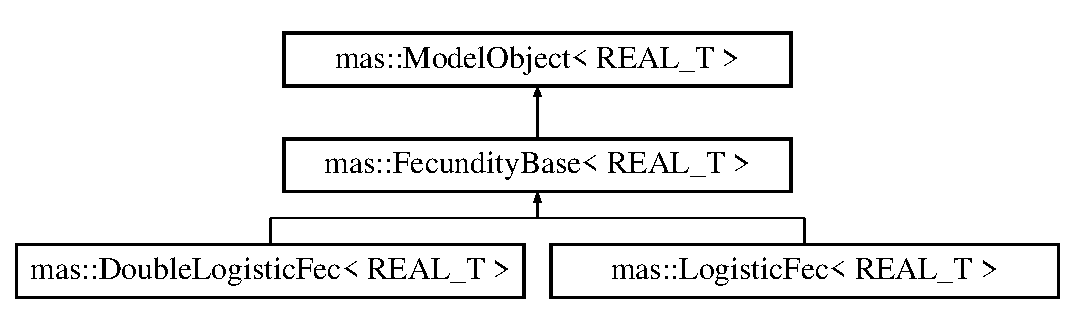
\includegraphics[height=3.000000cm]{structmas_1_1_fecundity_base}
\end{center}
\end{figure}
\subsection*{Public Types}
\begin{DoxyCompactItemize}
\item 
typedef \hyperlink{structmas_1_1_variable_trait}{Variable\-Trait}$<$ R\-E\-A\-L\-\_\-\-T $>$\\*
\-::\hyperlink{structmas_1_1_model_object_a4e62fdbb5826f8fac311262b888ab10a}{variable} \hyperlink{structmas_1_1_fecundity_base_a3428ef488b92ccfab67d455e87e3386b}{variable}
\end{DoxyCompactItemize}
\subsection*{Public Member Functions}
\begin{DoxyCompactItemize}
\item 
virtual const \hyperlink{structmas_1_1_model_object_a4e62fdbb5826f8fac311262b888ab10a}{variable} \hyperlink{structmas_1_1_fecundity_base_a44573d4082a65920010d9d20ed2d8e14}{Evaluate} (const int \&sex, const \hyperlink{structmas_1_1_model_object_a4e62fdbb5826f8fac311262b888ab10a}{variable} \&age)=0
\item 
virtual const std\-::string \hyperlink{structmas_1_1_fecundity_base_a5a0ca3b02791910dd012a30f1c2bf2a8}{Name} ()
\end{DoxyCompactItemize}
\subsection*{Additional Inherited Members}


\subsection{Detailed Description}
\subsubsection*{template$<$typename R\-E\-A\-L\-\_\-\-T$>$struct mas\-::\-Fecundity\-Base$<$ R\-E\-A\-L\-\_\-\-T $>$}



Definition at line 41 of file Fecundity.\-hpp.



\subsection{Member Typedef Documentation}
\hypertarget{structmas_1_1_fecundity_base_a3428ef488b92ccfab67d455e87e3386b}{\index{mas\-::\-Fecundity\-Base@{mas\-::\-Fecundity\-Base}!variable@{variable}}
\index{variable@{variable}!mas::FecundityBase@{mas\-::\-Fecundity\-Base}}
\subsubsection[{variable}]{\setlength{\rightskip}{0pt plus 5cm}template$<$typename R\-E\-A\-L\-\_\-\-T $>$ typedef {\bf Variable\-Trait}$<$R\-E\-A\-L\-\_\-\-T$>$\-::{\bf variable} {\bf mas\-::\-Fecundity\-Base}$<$ R\-E\-A\-L\-\_\-\-T $>$\-::{\bf variable}}}\label{structmas_1_1_fecundity_base_a3428ef488b92ccfab67d455e87e3386b}


Definition at line 43 of file Fecundity.\-hpp.



\subsection{Member Function Documentation}
\hypertarget{structmas_1_1_fecundity_base_a44573d4082a65920010d9d20ed2d8e14}{\index{mas\-::\-Fecundity\-Base@{mas\-::\-Fecundity\-Base}!Evaluate@{Evaluate}}
\index{Evaluate@{Evaluate}!mas::FecundityBase@{mas\-::\-Fecundity\-Base}}
\subsubsection[{Evaluate}]{\setlength{\rightskip}{0pt plus 5cm}template$<$typename R\-E\-A\-L\-\_\-\-T $>$ virtual const {\bf variable} {\bf mas\-::\-Fecundity\-Base}$<$ R\-E\-A\-L\-\_\-\-T $>$\-::Evaluate (
\begin{DoxyParamCaption}
\item[{const int \&}]{sex, }
\item[{const {\bf variable} \&}]{age}
\end{DoxyParamCaption}
)\hspace{0.3cm}{\ttfamily [pure virtual]}}}\label{structmas_1_1_fecundity_base_a44573d4082a65920010d9d20ed2d8e14}


Implemented in \hyperlink{structmas_1_1_double_logistic_fec_a732cf8310636c612ed4a6cf78079e03b}{mas\-::\-Double\-Logistic\-Fec$<$ R\-E\-A\-L\-\_\-\-T $>$}, and \hyperlink{structmas_1_1_logistic_fec_a39ba0a3a580b10ec1cf5ad2e3d24a029}{mas\-::\-Logistic\-Fec$<$ R\-E\-A\-L\-\_\-\-T $>$}.

\hypertarget{structmas_1_1_fecundity_base_a5a0ca3b02791910dd012a30f1c2bf2a8}{\index{mas\-::\-Fecundity\-Base@{mas\-::\-Fecundity\-Base}!Name@{Name}}
\index{Name@{Name}!mas::FecundityBase@{mas\-::\-Fecundity\-Base}}
\subsubsection[{Name}]{\setlength{\rightskip}{0pt plus 5cm}template$<$typename R\-E\-A\-L\-\_\-\-T $>$ virtual const std\-::string {\bf mas\-::\-Fecundity\-Base}$<$ R\-E\-A\-L\-\_\-\-T $>$\-::Name (
\begin{DoxyParamCaption}
{}
\end{DoxyParamCaption}
)\hspace{0.3cm}{\ttfamily [inline]}, {\ttfamily [virtual]}}}\label{structmas_1_1_fecundity_base_a5a0ca3b02791910dd012a30f1c2bf2a8}


Reimplemented in \hyperlink{structmas_1_1_double_logistic_fec_a08517ef4ed14c1dc4e6fdce9baafbae0}{mas\-::\-Double\-Logistic\-Fec$<$ R\-E\-A\-L\-\_\-\-T $>$}, and \hyperlink{structmas_1_1_logistic_fec_a2c6a92c26528208819f69dabc1859956}{mas\-::\-Logistic\-Fec$<$ R\-E\-A\-L\-\_\-\-T $>$}.



Definition at line 47 of file Fecundity.\-hpp.



The documentation for this struct was generated from the following file\-:\begin{DoxyCompactItemize}
\item 
/home/oppy/\-Net\-Beans\-Projects/mas/\hyperlink{_fecundity_8hpp}{Fecundity.\-hpp}\end{DoxyCompactItemize}

\hypertarget{structmas_1_1_fishing_mortality}{\section{mas\-:\-:Fishing\-Mortality$<$ R\-E\-A\-L\-\_\-\-T $>$ Struct Template Reference}
\label{structmas_1_1_fishing_mortality}\index{mas\-::\-Fishing\-Mortality$<$ R\-E\-A\-L\-\_\-\-T $>$@{mas\-::\-Fishing\-Mortality$<$ R\-E\-A\-L\-\_\-\-T $>$}}
}


{\ttfamily \#include $<$Mortality.\-hpp$>$}

Inheritance diagram for mas\-:\-:Fishing\-Mortality$<$ R\-E\-A\-L\-\_\-\-T $>$\-:\begin{figure}[H]
\begin{center}
\leavevmode
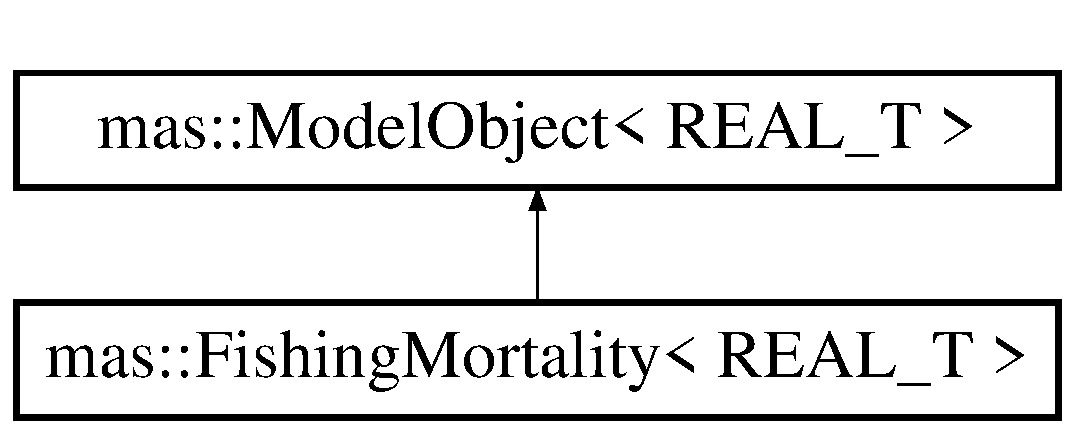
\includegraphics[height=2.000000cm]{structmas_1_1_fishing_mortality}
\end{center}
\end{figure}
\subsection*{Public Types}
\begin{DoxyCompactItemize}
\item 
typedef \hyperlink{structmas_1_1_variable_trait}{Variable\-Trait}$<$ R\-E\-A\-L\-\_\-\-T $>$\\*
\-::\hyperlink{structmas_1_1_fishing_mortality_ad7a9ae18fb1cbfe1bf7c2fa0b3e1ee73}{variable} \hyperlink{structmas_1_1_fishing_mortality_ad7a9ae18fb1cbfe1bf7c2fa0b3e1ee73}{variable}
\end{DoxyCompactItemize}
\subsection*{Public Member Functions}
\begin{DoxyCompactItemize}
\item 
const \hyperlink{structmas_1_1_fishing_mortality_ad7a9ae18fb1cbfe1bf7c2fa0b3e1ee73}{variable} \hyperlink{structmas_1_1_fishing_mortality_a9823a3d091ba0f9f5abf6f234d5bbe95}{Evaluate} (const int \&year, const int \&season)
\item 
\hyperlink{structmas_1_1_fishing_mortality_ad7a9ae18fb1cbfe1bf7c2fa0b3e1ee73}{variable} \& \hyperlink{structmas_1_1_fishing_mortality_a9ee4c943ac5a039e4e99a0f95ecd1b8f}{Get} (const int \&year, const int \&season)
\item 
void \hyperlink{structmas_1_1_fishing_mortality_a9571f43b68311da0487864c37943bc99}{Average\-Fmethod\-Contributions} ()
\item 
virtual std\-::string \hyperlink{structmas_1_1_fishing_mortality_a584a63c9d45ec427965f2d98c2a88c81}{To\-String} ()
\item 
virtual const std\-::string \hyperlink{structmas_1_1_fishing_mortality_ac76d1e34d6c062d090bc5265d100395d}{To\-J\-S\-O\-N\-String} ()
\item 
virtual const std\-::string \hyperlink{structmas_1_1_fishing_mortality_a32f715666745e58a7f24e5537b2ccf19}{Name} ()
\end{DoxyCompactItemize}
\subsection*{Public Attributes}
\begin{DoxyCompactItemize}
\item 
\hyperlink{namespacemas_aacd7136161d1e9de202129d69640a575}{Fishing\-Mortality\-Type} \hyperlink{structmas_1_1_fishing_mortality_aba52dc6a63a8c8bc895b946cba5a5309}{fishing\-\_\-mortality\-\_\-type} = \hyperlink{namespacemas_aacd7136161d1e9de202129d69640a575acd5f3e01a8588334bf98023c12ea8169}{E\-S\-T\-I\-M\-A\-T\-E\-D}
\item 
bool \hyperlink{structmas_1_1_fishing_mortality_aa5e8bbb289155d313e98aa8349dfdf2c}{needs\-\_\-delta\-\_\-method\-\_\-update} = false
\item 
R\-E\-A\-L\-\_\-\-T \hyperlink{structmas_1_1_fishing_mortality_ac9621f8a36e68bd04ff91a0896c4b09d}{contributions} = 0.\-0
\item 
std\-::vector$<$ std\-::vector\\*
$<$ \hyperlink{structmas_1_1_fishing_mortality_ad7a9ae18fb1cbfe1bf7c2fa0b3e1ee73}{variable} $>$ $>$ \hyperlink{structmas_1_1_fishing_mortality_a8762786de78be37776c371f1a4f46fcc}{fishing\-\_\-mortality}
\item 
std\-::unordered\-\_\-map$<$ int, \\*
std\-::unordered\-\_\-map$<$ int, \\*
std\-::vector$<$ std\-::vector\\*
$<$ \hyperlink{structmas_1_1_fishing_mortality_ad7a9ae18fb1cbfe1bf7c2fa0b3e1ee73}{variable} $>$ $>$ $>$ $>$ \hyperlink{structmas_1_1_fishing_mortality_ad92f2a24fd5a5f26a00ad98a9276af27}{f\-\_\-delta\-\_\-method\-\_\-at\-\_\-age}
\end{DoxyCompactItemize}


\subsection{Detailed Description}
\subsubsection*{template$<$typename R\-E\-A\-L\-\_\-\-T$>$struct mas\-::\-Fishing\-Mortality$<$ R\-E\-A\-L\-\_\-\-T $>$}



Definition at line 108 of file Mortality.\-hpp.



\subsection{Member Typedef Documentation}
\hypertarget{structmas_1_1_fishing_mortality_ad7a9ae18fb1cbfe1bf7c2fa0b3e1ee73}{\index{mas\-::\-Fishing\-Mortality@{mas\-::\-Fishing\-Mortality}!variable@{variable}}
\index{variable@{variable}!mas::FishingMortality@{mas\-::\-Fishing\-Mortality}}
\subsubsection[{variable}]{\setlength{\rightskip}{0pt plus 5cm}template$<$typename R\-E\-A\-L\-\_\-\-T $>$ typedef {\bf Variable\-Trait}$<$R\-E\-A\-L\-\_\-\-T$>$\-::{\bf variable} {\bf mas\-::\-Fishing\-Mortality}$<$ R\-E\-A\-L\-\_\-\-T $>$\-::{\bf variable}}}\label{structmas_1_1_fishing_mortality_ad7a9ae18fb1cbfe1bf7c2fa0b3e1ee73}


Definition at line 112 of file Mortality.\-hpp.



\subsection{Member Function Documentation}
\hypertarget{structmas_1_1_fishing_mortality_a9571f43b68311da0487864c37943bc99}{\index{mas\-::\-Fishing\-Mortality@{mas\-::\-Fishing\-Mortality}!Average\-Fmethod\-Contributions@{Average\-Fmethod\-Contributions}}
\index{Average\-Fmethod\-Contributions@{Average\-Fmethod\-Contributions}!mas::FishingMortality@{mas\-::\-Fishing\-Mortality}}
\subsubsection[{Average\-Fmethod\-Contributions}]{\setlength{\rightskip}{0pt plus 5cm}template$<$typename R\-E\-A\-L\-\_\-\-T $>$ void {\bf mas\-::\-Fishing\-Mortality}$<$ R\-E\-A\-L\-\_\-\-T $>$\-::Average\-Fmethod\-Contributions (
\begin{DoxyParamCaption}
{}
\end{DoxyParamCaption}
)\hspace{0.3cm}{\ttfamily [inline]}}}\label{structmas_1_1_fishing_mortality_a9571f43b68311da0487864c37943bc99}


Definition at line 124 of file Mortality.\-hpp.

\hypertarget{structmas_1_1_fishing_mortality_a9823a3d091ba0f9f5abf6f234d5bbe95}{\index{mas\-::\-Fishing\-Mortality@{mas\-::\-Fishing\-Mortality}!Evaluate@{Evaluate}}
\index{Evaluate@{Evaluate}!mas::FishingMortality@{mas\-::\-Fishing\-Mortality}}
\subsubsection[{Evaluate}]{\setlength{\rightskip}{0pt plus 5cm}template$<$typename R\-E\-A\-L\-\_\-\-T $>$ const {\bf variable} {\bf mas\-::\-Fishing\-Mortality}$<$ R\-E\-A\-L\-\_\-\-T $>$\-::Evaluate (
\begin{DoxyParamCaption}
\item[{const int \&}]{year, }
\item[{const int \&}]{season}
\end{DoxyParamCaption}
)\hspace{0.3cm}{\ttfamily [inline]}}}\label{structmas_1_1_fishing_mortality_a9823a3d091ba0f9f5abf6f234d5bbe95}


Definition at line 116 of file Mortality.\-hpp.

\hypertarget{structmas_1_1_fishing_mortality_a9ee4c943ac5a039e4e99a0f95ecd1b8f}{\index{mas\-::\-Fishing\-Mortality@{mas\-::\-Fishing\-Mortality}!Get@{Get}}
\index{Get@{Get}!mas::FishingMortality@{mas\-::\-Fishing\-Mortality}}
\subsubsection[{Get}]{\setlength{\rightskip}{0pt plus 5cm}template$<$typename R\-E\-A\-L\-\_\-\-T $>$ {\bf variable}\& {\bf mas\-::\-Fishing\-Mortality}$<$ R\-E\-A\-L\-\_\-\-T $>$\-::Get (
\begin{DoxyParamCaption}
\item[{const int \&}]{year, }
\item[{const int \&}]{season}
\end{DoxyParamCaption}
)\hspace{0.3cm}{\ttfamily [inline]}}}\label{structmas_1_1_fishing_mortality_a9ee4c943ac5a039e4e99a0f95ecd1b8f}


Definition at line 120 of file Mortality.\-hpp.

\hypertarget{structmas_1_1_fishing_mortality_a32f715666745e58a7f24e5537b2ccf19}{\index{mas\-::\-Fishing\-Mortality@{mas\-::\-Fishing\-Mortality}!Name@{Name}}
\index{Name@{Name}!mas::FishingMortality@{mas\-::\-Fishing\-Mortality}}
\subsubsection[{Name}]{\setlength{\rightskip}{0pt plus 5cm}template$<$typename R\-E\-A\-L\-\_\-\-T $>$ virtual const std\-::string {\bf mas\-::\-Fishing\-Mortality}$<$ R\-E\-A\-L\-\_\-\-T $>$\-::Name (
\begin{DoxyParamCaption}
{}
\end{DoxyParamCaption}
)\hspace{0.3cm}{\ttfamily [inline]}, {\ttfamily [virtual]}}}\label{structmas_1_1_fishing_mortality_a32f715666745e58a7f24e5537b2ccf19}


Definition at line 220 of file Mortality.\-hpp.

\hypertarget{structmas_1_1_fishing_mortality_ac76d1e34d6c062d090bc5265d100395d}{\index{mas\-::\-Fishing\-Mortality@{mas\-::\-Fishing\-Mortality}!To\-J\-S\-O\-N\-String@{To\-J\-S\-O\-N\-String}}
\index{To\-J\-S\-O\-N\-String@{To\-J\-S\-O\-N\-String}!mas::FishingMortality@{mas\-::\-Fishing\-Mortality}}
\subsubsection[{To\-J\-S\-O\-N\-String}]{\setlength{\rightskip}{0pt plus 5cm}template$<$typename R\-E\-A\-L\-\_\-\-T $>$ virtual const std\-::string {\bf mas\-::\-Fishing\-Mortality}$<$ R\-E\-A\-L\-\_\-\-T $>$\-::To\-J\-S\-O\-N\-String (
\begin{DoxyParamCaption}
{}
\end{DoxyParamCaption}
)\hspace{0.3cm}{\ttfamily [inline]}, {\ttfamily [virtual]}}}\label{structmas_1_1_fishing_mortality_ac76d1e34d6c062d090bc5265d100395d}


Reimplemented from \hyperlink{structmas_1_1_model_object_af40b3c89b11919fc5aea21dcf1cd027b}{mas\-::\-Model\-Object$<$ R\-E\-A\-L\-\_\-\-T $>$}.



Definition at line 155 of file Mortality.\-hpp.

\hypertarget{structmas_1_1_fishing_mortality_a584a63c9d45ec427965f2d98c2a88c81}{\index{mas\-::\-Fishing\-Mortality@{mas\-::\-Fishing\-Mortality}!To\-String@{To\-String}}
\index{To\-String@{To\-String}!mas::FishingMortality@{mas\-::\-Fishing\-Mortality}}
\subsubsection[{To\-String}]{\setlength{\rightskip}{0pt plus 5cm}template$<$typename R\-E\-A\-L\-\_\-\-T $>$ virtual std\-::string {\bf mas\-::\-Fishing\-Mortality}$<$ R\-E\-A\-L\-\_\-\-T $>$\-::To\-String (
\begin{DoxyParamCaption}
{}
\end{DoxyParamCaption}
)\hspace{0.3cm}{\ttfamily [inline]}, {\ttfamily [virtual]}}}\label{structmas_1_1_fishing_mortality_a584a63c9d45ec427965f2d98c2a88c81}


Reimplemented from \hyperlink{structmas_1_1_model_object_a8eaf6c7c52e42ea8869aefa318358cb5}{mas\-::\-Model\-Object$<$ R\-E\-A\-L\-\_\-\-T $>$}.



Definition at line 140 of file Mortality.\-hpp.



\subsection{Member Data Documentation}
\hypertarget{structmas_1_1_fishing_mortality_ac9621f8a36e68bd04ff91a0896c4b09d}{\index{mas\-::\-Fishing\-Mortality@{mas\-::\-Fishing\-Mortality}!contributions@{contributions}}
\index{contributions@{contributions}!mas::FishingMortality@{mas\-::\-Fishing\-Mortality}}
\subsubsection[{contributions}]{\setlength{\rightskip}{0pt plus 5cm}template$<$typename R\-E\-A\-L\-\_\-\-T $>$ R\-E\-A\-L\-\_\-\-T {\bf mas\-::\-Fishing\-Mortality}$<$ R\-E\-A\-L\-\_\-\-T $>$\-::contributions = 0.\-0}}\label{structmas_1_1_fishing_mortality_ac9621f8a36e68bd04ff91a0896c4b09d}


Definition at line 111 of file Mortality.\-hpp.

\hypertarget{structmas_1_1_fishing_mortality_ad92f2a24fd5a5f26a00ad98a9276af27}{\index{mas\-::\-Fishing\-Mortality@{mas\-::\-Fishing\-Mortality}!f\-\_\-delta\-\_\-method\-\_\-at\-\_\-age@{f\-\_\-delta\-\_\-method\-\_\-at\-\_\-age}}
\index{f\-\_\-delta\-\_\-method\-\_\-at\-\_\-age@{f\-\_\-delta\-\_\-method\-\_\-at\-\_\-age}!mas::FishingMortality@{mas\-::\-Fishing\-Mortality}}
\subsubsection[{f\-\_\-delta\-\_\-method\-\_\-at\-\_\-age}]{\setlength{\rightskip}{0pt plus 5cm}template$<$typename R\-E\-A\-L\-\_\-\-T $>$ std\-::unordered\-\_\-map$<$int, std\-::unordered\-\_\-map$<$int, std\-::vector$<$std\-::vector$<${\bf variable}$>$ $>$ $>$ $>$ {\bf mas\-::\-Fishing\-Mortality}$<$ R\-E\-A\-L\-\_\-\-T $>$\-::f\-\_\-delta\-\_\-method\-\_\-at\-\_\-age}}\label{structmas_1_1_fishing_mortality_ad92f2a24fd5a5f26a00ad98a9276af27}


Definition at line 114 of file Mortality.\-hpp.

\hypertarget{structmas_1_1_fishing_mortality_a8762786de78be37776c371f1a4f46fcc}{\index{mas\-::\-Fishing\-Mortality@{mas\-::\-Fishing\-Mortality}!fishing\-\_\-mortality@{fishing\-\_\-mortality}}
\index{fishing\-\_\-mortality@{fishing\-\_\-mortality}!mas::FishingMortality@{mas\-::\-Fishing\-Mortality}}
\subsubsection[{fishing\-\_\-mortality}]{\setlength{\rightskip}{0pt plus 5cm}template$<$typename R\-E\-A\-L\-\_\-\-T $>$ std\-::vector$<$std\-::vector$<${\bf variable}$>$ $>$ {\bf mas\-::\-Fishing\-Mortality}$<$ R\-E\-A\-L\-\_\-\-T $>$\-::fishing\-\_\-mortality}}\label{structmas_1_1_fishing_mortality_a8762786de78be37776c371f1a4f46fcc}


Definition at line 113 of file Mortality.\-hpp.

\hypertarget{structmas_1_1_fishing_mortality_aba52dc6a63a8c8bc895b946cba5a5309}{\index{mas\-::\-Fishing\-Mortality@{mas\-::\-Fishing\-Mortality}!fishing\-\_\-mortality\-\_\-type@{fishing\-\_\-mortality\-\_\-type}}
\index{fishing\-\_\-mortality\-\_\-type@{fishing\-\_\-mortality\-\_\-type}!mas::FishingMortality@{mas\-::\-Fishing\-Mortality}}
\subsubsection[{fishing\-\_\-mortality\-\_\-type}]{\setlength{\rightskip}{0pt plus 5cm}template$<$typename R\-E\-A\-L\-\_\-\-T $>$ {\bf Fishing\-Mortality\-Type} {\bf mas\-::\-Fishing\-Mortality}$<$ R\-E\-A\-L\-\_\-\-T $>$\-::fishing\-\_\-mortality\-\_\-type = {\bf E\-S\-T\-I\-M\-A\-T\-E\-D}}}\label{structmas_1_1_fishing_mortality_aba52dc6a63a8c8bc895b946cba5a5309}


Definition at line 109 of file Mortality.\-hpp.

\hypertarget{structmas_1_1_fishing_mortality_aa5e8bbb289155d313e98aa8349dfdf2c}{\index{mas\-::\-Fishing\-Mortality@{mas\-::\-Fishing\-Mortality}!needs\-\_\-delta\-\_\-method\-\_\-update@{needs\-\_\-delta\-\_\-method\-\_\-update}}
\index{needs\-\_\-delta\-\_\-method\-\_\-update@{needs\-\_\-delta\-\_\-method\-\_\-update}!mas::FishingMortality@{mas\-::\-Fishing\-Mortality}}
\subsubsection[{needs\-\_\-delta\-\_\-method\-\_\-update}]{\setlength{\rightskip}{0pt plus 5cm}template$<$typename R\-E\-A\-L\-\_\-\-T $>$ bool {\bf mas\-::\-Fishing\-Mortality}$<$ R\-E\-A\-L\-\_\-\-T $>$\-::needs\-\_\-delta\-\_\-method\-\_\-update = false}}\label{structmas_1_1_fishing_mortality_aa5e8bbb289155d313e98aa8349dfdf2c}


Definition at line 110 of file Mortality.\-hpp.



The documentation for this struct was generated from the following file\-:\begin{DoxyCompactItemize}
\item 
/home/oppy/\-Net\-Beans\-Projects/mas/\hyperlink{_mortality_8hpp}{Mortality.\-hpp}\end{DoxyCompactItemize}

\hypertarget{structmas_1_1_fleet}{\section{mas\-:\-:Fleet$<$ R\-E\-A\-L\-\_\-\-T $>$ Struct Template Reference}
\label{structmas_1_1_fleet}\index{mas\-::\-Fleet$<$ R\-E\-A\-L\-\_\-\-T $>$@{mas\-::\-Fleet$<$ R\-E\-A\-L\-\_\-\-T $>$}}
}


{\ttfamily \#include $<$Fleet.\-hpp$>$}

Inheritance diagram for mas\-:\-:Fleet$<$ R\-E\-A\-L\-\_\-\-T $>$\-:\begin{figure}[H]
\begin{center}
\leavevmode
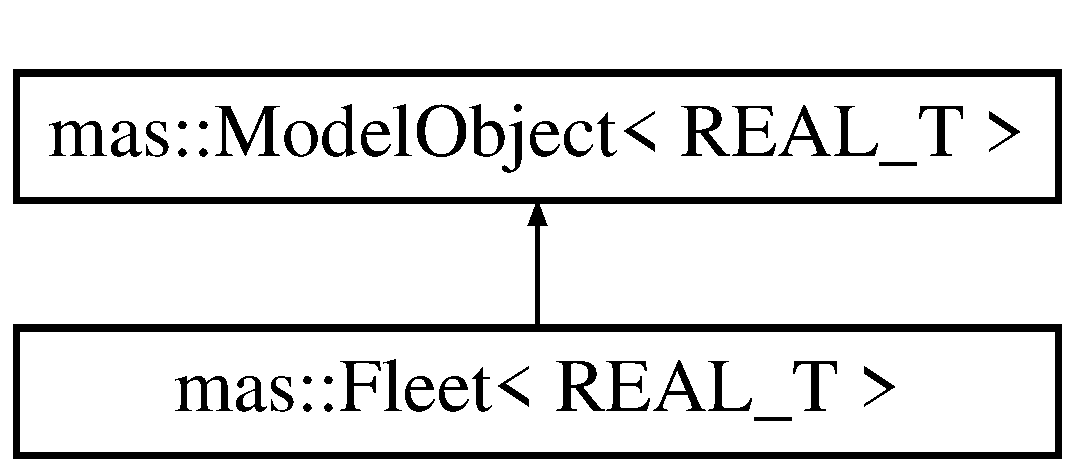
\includegraphics[height=2.000000cm]{structmas_1_1_fleet}
\end{center}
\end{figure}
\subsection*{Public Types}
\begin{DoxyCompactItemize}
\item 
typedef \hyperlink{structmas_1_1_variable_trait}{Variable\-Trait}$<$ R\-E\-A\-L\-\_\-\-T $>$\\*
\-::\hyperlink{structmas_1_1_fleet_a1902d0842cb7ce9b9bdd4be013e709a9}{variable} \hyperlink{structmas_1_1_fleet_a1902d0842cb7ce9b9bdd4be013e709a9}{variable}
\item 
typedef std\-::unordered\-\_\-map\\*
$<$ int, std\-::unordered\-\_\-map$<$ int, \\*
int $>$ $>$\-::iterator \hyperlink{structmas_1_1_fleet_aadb49821d696137325793eec3abdde87}{season\-\_\-area\-\_\-selectivity\-\_\-ids\-\_\-iterator}
\item 
typedef std\-::unordered\-\_\-map\\*
$<$ int, std\-::shared\-\_\-ptr\\*
$<$ \hyperlink{structmas_1_1_selectivity_base}{mas\-::\-Selectivity\-Base}$<$ R\-E\-A\-L\-\_\-\-T $>$\\*
 $>$ $>$\-::iterator \hyperlink{structmas_1_1_fleet_a7754c30a6a70e4bac646b59fb93db23e}{area\-\_\-sectivity\-\_\-iterator}
\item 
typedef std\-::unordered\-\_\-map\\*
$<$ int, std\-::unordered\-\_\-map$<$ int, \\*
int $>$ $>$\-::iterator \hyperlink{structmas_1_1_fleet_ad3f5709dbe6c7d4b2d9082783272a48a}{season\-\_\-area\-\_\-id\-\_\-iterator}
\item 
typedef std\-::unordered\-\_\-map\\*
$<$ int, int $>$\-::iterator \hyperlink{structmas_1_1_fleet_ac0ff17aa69ffb817ba0d36aa19b42277}{area\-\_\-id\-\_\-iterator}
\item 
typedef std\-::unordered\-\_\-map\\*
$<$ int, int $>$\-::iterator \hyperlink{structmas_1_1_fleet_a28ea634c7029c6e00c6362c152d0ac7a}{season\-\_\-id\-\_\-iterator}
\item 
typedef std\-::unordered\-\_\-map\\*
$<$ int, std\-::unordered\-\_\-map$<$ int, \\*
std\-::shared\-\_\-ptr\\*
$<$ \hyperlink{structmas_1_1_selectivity_base}{mas\-::\-Selectivity\-Base}$<$ R\-E\-A\-L\-\_\-\-T $>$\\*
 $>$ $>$ $>$\-::iterator \hyperlink{structmas_1_1_fleet_af276dbe3918638c6bc4556bd97330939}{season\-\_\-area\-\_\-selectivity\-\_\-iterator}
\item 
typedef std\-::unordered\-\_\-map\\*
$<$ int, std\-::unordered\-\_\-map$<$ int, \\*
std\-::shared\-\_\-ptr\\*
$<$ \hyperlink{structmas_1_1_fishing_mortality}{mas\-::\-Fishing\-Mortality}\\*
$<$ R\-E\-A\-L\-\_\-\-T $>$ $>$ $>$ $>$\-::iterator \hyperlink{structmas_1_1_fleet_aab7bbd15fe8e99db584f6d936c028bf3}{season\-\_\-area\-\_\-fishing\-\_\-mortality\-\_\-iterator}
\item 
typedef std\-::unordered\-\_\-map\\*
$<$ int, std\-::shared\-\_\-ptr\\*
$<$ \hyperlink{structmas_1_1_fishing_mortality}{mas\-::\-Fishing\-Mortality}\\*
$<$ R\-E\-A\-L\-\_\-\-T $>$ $>$ $>$\-::iterator \hyperlink{structmas_1_1_fleet_a72800f7ad0b8ec91f129bd8020c19912}{area\-\_\-fishing\-\_\-mortality\-\_\-iterator}
\item 
typedef std\-::unordered\-\_\-map\\*
$<$ int, std\-::shared\-\_\-ptr\\*
$<$ \hyperlink{structmas_1_1_fishing_mortality}{mas\-::\-Fishing\-Mortality}\\*
$<$ R\-E\-A\-L\-\_\-\-T $>$ $>$ $>$\-::iterator \hyperlink{structmas_1_1_fleet_a446379b7a809ae7e2dd208c577e87a20}{delta\-\_\-method\-\_\-fishing\-\_\-mortality\-\_\-iterator}
\end{DoxyCompactItemize}
\subsection*{Public Member Functions}
\begin{DoxyCompactItemize}
\item 
void \hyperlink{structmas_1_1_fleet_a179636161da4b8c126d3afd1b7ea6edd}{Initialize} (size\-\_\-t \hyperlink{structmas_1_1_fleet_a823238fd7eb794d49a64743395bf1ae5}{years}, size\-\_\-t \hyperlink{structmas_1_1_fleet_a389f70f4bb3190303aba1ae9aca8c018}{seasons}, size\-\_\-t \hyperlink{structmas_1_1_fleet_adc63e3bd51a0e1897fba4c726f7ca8f8}{ages})
\item 
void \hyperlink{structmas_1_1_fleet_a54693c200e2a03dfd1dc36cbdbfab912}{Initialize\-N\-L\-L\-Components} ()
\item 
void \hyperlink{structmas_1_1_fleet_aa131029e55eb68d71f6b65b4ddea485a}{Prepare} ()
\item 
void \hyperlink{structmas_1_1_fleet_ae1e568c71625f18513261850e4a78236}{Initialize\-Fishing\-Mortality} ()
\item 
bool \hyperlink{structmas_1_1_fleet_a1c931c611ed3b073606e95f028508703}{Operates\-In\-Area} (int area)
\item 
void \hyperlink{structmas_1_1_fleet_a2539b0783335bf2121a5c841da94d321}{Compute\-Proportions} ()
\item 
void \hyperlink{structmas_1_1_fleet_ab82761b712d8029a6cb0712e8a7964bd}{Compute\-N\-L\-L\-Components} ()
\item 
void \hyperlink{structmas_1_1_fleet_a9fd5e000daf896b61cf6bd01e5ba2bd4}{Compute\-Goodness\-Of\-Fit} ()
\item 
void \hyperlink{structmas_1_1_fleet_aa147d8f74e9976533fef4aa99b01a540}{Evaluate\-Biomass\-Component} (int year, int season)
\item 
void \hyperlink{structmas_1_1_fleet_aedb94a407107c79e0d4c134f9bba3502}{Evaluate\-Age\-Comp\-Component} (int year, int season)
\item 
virtual const std\-::string \hyperlink{structmas_1_1_fleet_a438089d58f104668621d9426fa1e1c86}{To\-J\-S\-O\-N\-String} ()
\end{DoxyCompactItemize}
\subsection*{Public Attributes}
\begin{DoxyCompactItemize}
\item 
\hyperlink{structmas_1_1_fleet_a1902d0842cb7ce9b9bdd4be013e709a9}{variable} \hyperlink{structmas_1_1_fleet_a940dd1929ae7d8efec755542a0462e45}{f}
\item 
std\-::string \hyperlink{structmas_1_1_fleet_a4c22a8ff3dfa7b1a7684afccfc461c54}{name}
\item 
int \hyperlink{structmas_1_1_fleet_a823238fd7eb794d49a64743395bf1ae5}{years}
\item 
int \hyperlink{structmas_1_1_fleet_a389f70f4bb3190303aba1ae9aca8c018}{seasons}
\item 
int \hyperlink{structmas_1_1_fleet_adc63e3bd51a0e1897fba4c726f7ca8f8}{ages}
\item 
bool \hyperlink{structmas_1_1_fleet_a983d40b11fbaef98245d435a6420f162}{has\-\_\-catch\-\_\-data\-\_\-annual\-\_\-biomass}
\item 
bool \hyperlink{structmas_1_1_fleet_aab0d326e2e7fb03bcd5a8073b526c255}{has\-\_\-catch\-\_\-data\-\_\-biomass\-\_\-time\-\_\-by\-\_\-age}
\item 
bool \hyperlink{structmas_1_1_fleet_ab292045bcb9dd21ab25a0b6f2404e351}{has\-\_\-catch\-\_\-data\-\_\-numbers\-\_\-at\-\_\-age}
\item 
bool \hyperlink{structmas_1_1_fleet_af74c0ec58026828cd286f6f4c317e517}{has\-\_\-catch\-\_\-data\-\_\-proportion\-\_\-at\-\_\-age}
\item 
std\-::shared\-\_\-ptr$<$ \hyperlink{structmas_1_1_data_object}{Data\-Object}\\*
$<$ R\-E\-A\-L\-\_\-\-T $>$ $>$ \hyperlink{structmas_1_1_fleet_a996dcf8ffd91799f62cf2421d81eaac0}{catch\-\_\-biomass\-\_\-data}
\item 
std\-::shared\-\_\-ptr$<$ \hyperlink{structmas_1_1_data_object}{Data\-Object}\\*
$<$ R\-E\-A\-L\-\_\-\-T $>$ $>$ \hyperlink{structmas_1_1_fleet_a39314db6371bbf66ec72d41e871e6eca}{catch\-\_\-proportion\-\_\-at\-\_\-age\-\_\-data\-\_\-\-N}
\item 
std\-::shared\-\_\-ptr$<$ \hyperlink{structmas_1_1_data_object}{Data\-Object}\\*
$<$ R\-E\-A\-L\-\_\-\-T $>$ $>$ \hyperlink{structmas_1_1_fleet_ae6c54a589f2e6cbdb413e3759bffca5d}{catch\-\_\-proportion\-\_\-at\-\_\-age\-\_\-data}
\item 
std\-::shared\-\_\-ptr$<$ \hyperlink{structmas_1_1_data_object}{Data\-Object}\\*
$<$ R\-E\-A\-L\-\_\-\-T $>$ $>$ \hyperlink{structmas_1_1_fleet_a5bacb0578a3e651fc28a8ba2d233a14b}{catch\-\_\-proportion\-\_\-at\-\_\-length\-\_\-data\-\_\-\-N}
\item 
std\-::shared\-\_\-ptr$<$ \hyperlink{structmas_1_1_data_object}{Data\-Object}\\*
$<$ R\-E\-A\-L\-\_\-\-T $>$ $>$ \hyperlink{structmas_1_1_fleet_ae18e627f80c8ca519535bfc90d9634b5}{catch\-\_\-proportion\-\_\-at\-\_\-length\-\_\-data}
\item 
std\-::shared\-\_\-ptr$<$ \hyperlink{structmas_1_1_data_object}{Data\-Object}\\*
$<$ R\-E\-A\-L\-\_\-\-T $>$ $>$ \hyperlink{structmas_1_1_fleet_a46862ac16c8d360c9290dad74aee9a17}{catch\-\_\-mean\-\_\-size\-\_\-at\-\_\-age\-\_\-data}
\item 
std\-::shared\-\_\-ptr$<$ \hyperlink{structmas_1_1_data_object}{Data\-Object}\\*
$<$ R\-E\-A\-L\-\_\-\-T $>$ $>$ \hyperlink{structmas_1_1_fleet_acc8b3609ca90f6efd5801fb8820777f8}{catch\-\_\-mean\-\_\-weight\-\_\-at\-\_\-age\-\_\-data}
\item 
std\-::vector$<$ std\-::shared\-\_\-ptr\\*
$<$ \hyperlink{structmas_1_1_data_object}{Data\-Object}$<$ R\-E\-A\-L\-\_\-\-T $>$ $>$ $>$ \hyperlink{structmas_1_1_fleet_a9b5dca826b2d1b7b05a705b903a27fad}{data\-\_\-objects}
\item 
int \hyperlink{structmas_1_1_fleet_aa87c827150245f5859ca47fc303eceb8}{fishery\-\_\-age\-\_\-comp\-\_\-likelihood\-\_\-component\-\_\-id} = -\/999
\item 
std\-::shared\-\_\-ptr\\*
$<$ \hyperlink{structmas_1_1_n_l_l_functor}{mas\-::\-N\-L\-L\-Functor}$<$ R\-E\-A\-L\-\_\-\-T $>$ $>$ \hyperlink{structmas_1_1_fleet_ae0e54dbe1514b3d5a33293b4250e0be4}{fishery\-\_\-age\-\_\-comp\-\_\-likelihood\-\_\-component}
\item 
int \hyperlink{structmas_1_1_fleet_a2f3667e571a5c22538606e4c3156f7b5}{fishery\-\_\-biomass\-\_\-likelihood\-\_\-component\-\_\-id} = -\/999
\item 
std\-::shared\-\_\-ptr\\*
$<$ \hyperlink{structmas_1_1_n_l_l_functor}{mas\-::\-N\-L\-L\-Functor}$<$ R\-E\-A\-L\-\_\-\-T $>$ $>$ \hyperlink{structmas_1_1_fleet_abd3235a7cfd42c0106c59e8b51f4671d}{fishery\-\_\-biomass\-\_\-likelihood\-\_\-component}
\item 
std\-::unordered\-\_\-set$<$ int $>$ \hyperlink{structmas_1_1_fleet_aaa8ca2ea30b1afee976199eaabd6caa0}{operational\-\_\-areas}
\item 
std\-::unordered\-\_\-map$<$ int, \\*
std\-::unordered\-\_\-map$<$ int, int $>$ $>$ \hyperlink{structmas_1_1_fleet_a2c2c1b323ec7845085ebe105b5f64096}{season\-\_\-area\-\_\-selectivity\-\_\-ids}
\item 
std\-::unordered\-\_\-map$<$ int, \\*
std\-::unordered\-\_\-map$<$ int, \\*
std\-::shared\-\_\-ptr\\*
$<$ \hyperlink{structmas_1_1_selectivity_base}{mas\-::\-Selectivity\-Base}$<$ R\-E\-A\-L\-\_\-\-T $>$ $>$ $>$ $>$ \hyperlink{structmas_1_1_fleet_aa8e734855b66757bf86314f6ae76878c}{season\-\_\-area\-\_\-selectivity}
\item 
std\-::unordered\-\_\-map$<$ int, \\*
std\-::unordered\-\_\-map$<$ int, int $>$ $>$ \hyperlink{structmas_1_1_fleet_ac13bc4011086cb3fc3b6838d02885db5}{area\-\_\-season\-\_\-selectivity\-\_\-ids}
\item 
std\-::unordered\-\_\-map$<$ int, \\*
std\-::unordered\-\_\-map$<$ int, \\*
std\-::shared\-\_\-ptr\\*
$<$ \hyperlink{structmas_1_1_selectivity_base}{mas\-::\-Selectivity\-Base}$<$ R\-E\-A\-L\-\_\-\-T $>$ $>$ $>$ $>$ \hyperlink{structmas_1_1_fleet_a0cf9a3f0c5ae179699c1264a7583db56}{area\-\_\-season\-\_\-selectivity}
\item 
std\-::unordered\-\_\-map$<$ int, \\*
std\-::unordered\-\_\-map$<$ int, int $>$ $>$ \hyperlink{structmas_1_1_fleet_a31e805b1616d5a216530b48ea154c973}{area\-\_\-season\-\_\-fishing\-\_\-mortality\-\_\-ids}
\item 
std\-::unordered\-\_\-map$<$ int, \\*
std\-::unordered\-\_\-map$<$ int, \\*
std\-::shared\-\_\-ptr\\*
$<$ \hyperlink{structmas_1_1_fishing_mortality}{mas\-::\-Fishing\-Mortality}\\*
$<$ R\-E\-A\-L\-\_\-\-T $>$ $>$ $>$ $>$ \hyperlink{structmas_1_1_fleet_a5fbc6ef08467142e1797a26f557481e8}{area\-\_\-season\-\_\-fishing\-\_\-mortality}
\item 
std\-::unordered\-\_\-map$<$ int, \\*
std\-::unordered\-\_\-map$<$ int, int $>$ $>$ \hyperlink{structmas_1_1_fleet_acab7b946bf0d12476d4167f9d35693e8}{season\-\_\-area\-\_\-fishing\-\_\-mortality\-\_\-ids}
\item 
std\-::unordered\-\_\-map$<$ int, \\*
std\-::unordered\-\_\-map$<$ int, \\*
std\-::shared\-\_\-ptr\\*
$<$ \hyperlink{structmas_1_1_fishing_mortality}{mas\-::\-Fishing\-Mortality}\\*
$<$ R\-E\-A\-L\-\_\-\-T $>$ $>$ $>$ $>$ \hyperlink{structmas_1_1_fleet_a2eba2d477fe351f44a1c22f51f75018f}{season\-\_\-area\-\_\-fishing\-\_\-mortality}
\item 
std\-::unordered\-\_\-map$<$ int, \\*
std\-::shared\-\_\-ptr\\*
$<$ \hyperlink{structmas_1_1_fishing_mortality}{mas\-::\-Fishing\-Mortality}\\*
$<$ R\-E\-A\-L\-\_\-\-T $>$ $>$ $>$ \hyperlink{structmas_1_1_fleet_afd6e03157a9ad766993a41d4eb61124c}{delta\-\_\-method\-\_\-fishing\-\_\-mortality}
\item 
std\-::vector$<$ \hyperlink{structmas_1_1_fleet_a1902d0842cb7ce9b9bdd4be013e709a9}{variable} $>$ \hyperlink{structmas_1_1_fleet_aec96c786b81fb4cf0d908de0297cc2f4}{catch\-\_\-biomass\-\_\-total}
\item 
std\-::vector$<$ \hyperlink{structmas_1_1_fleet_a1902d0842cb7ce9b9bdd4be013e709a9}{variable} $>$ \hyperlink{structmas_1_1_fleet_a9ff1f7b831b4297a0241ce24f83b9e0f}{catch\-\_\-biomass\-\_\-total\-\_\-males}
\item 
std\-::vector$<$ \hyperlink{structmas_1_1_fleet_a1902d0842cb7ce9b9bdd4be013e709a9}{variable} $>$ \hyperlink{structmas_1_1_fleet_a25f8a76ca51ac7bf920d94d8d3c122c7}{catch\-\_\-biomass\-\_\-total\-\_\-females}
\item 
std\-::vector$<$ \hyperlink{structmas_1_1_fleet_a1902d0842cb7ce9b9bdd4be013e709a9}{variable} $>$ \hyperlink{structmas_1_1_fleet_a1f88d8e497852415b1e4010f8ab4d18f}{numbers\-\_\-at\-\_\-age}
\item 
std\-::vector$<$ \hyperlink{structmas_1_1_fleet_a1902d0842cb7ce9b9bdd4be013e709a9}{variable} $>$ \hyperlink{structmas_1_1_fleet_ad7457fd4d7e459925b87d50dc591b04c}{numbers\-\_\-total}
\item 
std\-::vector$<$ \hyperlink{structmas_1_1_fleet_a1902d0842cb7ce9b9bdd4be013e709a9}{variable} $>$ \hyperlink{structmas_1_1_fleet_a19e63403b6cc924ffbbf4876fdeb1cd0}{proportion\-\_\-at\-\_\-age}
\item 
std\-::vector$<$ \hyperlink{structmas_1_1_fleet_a1902d0842cb7ce9b9bdd4be013e709a9}{variable} $>$ \hyperlink{structmas_1_1_fleet_ad4ec4a206dbb1af192c85ae7ab0929ea}{catch\-\_\-proportion\-\_\-at\-\_\-age}
\item 
std\-::vector$<$ \hyperlink{structmas_1_1_fleet_a1902d0842cb7ce9b9bdd4be013e709a9}{variable} $>$ \hyperlink{structmas_1_1_fleet_ab29452b064132572243fbbb6ce7e8c06}{catch\-\_\-biomass\-\_\-proportion\-\_\-at\-\_\-age}
\item 
std\-::vector$<$ \hyperlink{structmas_1_1_fleet_a1902d0842cb7ce9b9bdd4be013e709a9}{variable} $>$ \hyperlink{structmas_1_1_fleet_a2a423b2624e36ff6ff786b4bea5db2fe}{catch\-\_\-at\-\_\-age}
\item 
std\-::unordered\-\_\-map$<$ int, \\*
std\-::unordered\-\_\-map$<$ int, \\*
std\-::vector$<$ \hyperlink{structmas_1_1_fleet_a1902d0842cb7ce9b9bdd4be013e709a9}{variable} $>$ $>$ $>$ \hyperlink{structmas_1_1_fleet_a5a9769854c2272ced6396dc091b3e318}{f\-\_\-at\-\_\-age}
\item 
std\-::unordered\-\_\-map$<$ int, \\*
std\-::unordered\-\_\-map$<$ int, \\*
std\-::vector$<$ \hyperlink{structmas_1_1_fleet_a1902d0842cb7ce9b9bdd4be013e709a9}{variable} $>$ $>$ $>$ \hyperlink{structmas_1_1_fleet_a0bd290f2fba5bd5f00a1666673d77a3b}{z\-\_\-at\-\_\-age}
\item 
std\-::vector$<$ \hyperlink{structmas_1_1_fleet_a1902d0842cb7ce9b9bdd4be013e709a9}{variable} $>$ \hyperlink{structmas_1_1_fleet_a6bcc185d0581e22288665272df90d8a0}{catch\-\_\-biomass\-\_\-at\-\_\-age}
\item 
std\-::vector$<$ \hyperlink{structmas_1_1_fleet_a1902d0842cb7ce9b9bdd4be013e709a9}{variable} $>$ \hyperlink{structmas_1_1_fleet_aa4aa9e9a3d34fc15d15543ae02aea2bd}{numbers\-\_\-at\-\_\-age\-\_\-males}
\item 
std\-::vector$<$ \hyperlink{structmas_1_1_fleet_a1902d0842cb7ce9b9bdd4be013e709a9}{variable} $>$ \hyperlink{structmas_1_1_fleet_a40064758c90639b12944f9ef12aeaf01}{numbers\-\_\-total\-\_\-males}
\item 
std\-::vector$<$ \hyperlink{structmas_1_1_fleet_a1902d0842cb7ce9b9bdd4be013e709a9}{variable} $>$ \hyperlink{structmas_1_1_fleet_a8a3bf314e6f6249f84fdaded007a0067}{proportion\-\_\-at\-\_\-age\-\_\-males}
\item 
std\-::vector$<$ \hyperlink{structmas_1_1_fleet_a1902d0842cb7ce9b9bdd4be013e709a9}{variable} $>$ \hyperlink{structmas_1_1_fleet_a03a9617218d69139a286073025084dbd}{catch\-\_\-proportion\-\_\-at\-\_\-age\-\_\-males}
\item 
std\-::vector$<$ \hyperlink{structmas_1_1_fleet_a1902d0842cb7ce9b9bdd4be013e709a9}{variable} $>$ \hyperlink{structmas_1_1_fleet_aa15871c1252f3fc4f0d5eb19376ef18c}{catch\-\_\-biomass\-\_\-proportion\-\_\-at\-\_\-age\-\_\-males}
\item 
std\-::vector$<$ \hyperlink{structmas_1_1_fleet_a1902d0842cb7ce9b9bdd4be013e709a9}{variable} $>$ \hyperlink{structmas_1_1_fleet_a384cc77fb80ba8d2d91722468839ea5d}{catch\-\_\-at\-\_\-age\-\_\-males}
\item 
std\-::unordered\-\_\-map$<$ int, \\*
std\-::unordered\-\_\-map$<$ int, \\*
std\-::vector$<$ \hyperlink{structmas_1_1_fleet_a1902d0842cb7ce9b9bdd4be013e709a9}{variable} $>$ $>$ $>$ \hyperlink{structmas_1_1_fleet_a1019367ebec70e8480fa5bcf76851d6f}{f\-\_\-at\-\_\-age\-\_\-males}
\item 
std\-::unordered\-\_\-map$<$ int, \\*
std\-::unordered\-\_\-map$<$ int, \\*
std\-::vector$<$ \hyperlink{structmas_1_1_fleet_a1902d0842cb7ce9b9bdd4be013e709a9}{variable} $>$ $>$ $>$ \hyperlink{structmas_1_1_fleet_a177b878b912cd2c01729070c46e0f27d}{z\-\_\-at\-\_\-age\-\_\-males}
\item 
std\-::vector$<$ \hyperlink{structmas_1_1_fleet_a1902d0842cb7ce9b9bdd4be013e709a9}{variable} $>$ \hyperlink{structmas_1_1_fleet_a21e595437d97bf9d2197cf2bdddcc7a0}{catch\-\_\-biomass\-\_\-at\-\_\-age\-\_\-males}
\item 
std\-::vector$<$ \hyperlink{structmas_1_1_fleet_a1902d0842cb7ce9b9bdd4be013e709a9}{variable} $>$ \hyperlink{structmas_1_1_fleet_afbe9209cae969e13ee6480efab603e02}{numbers\-\_\-at\-\_\-age\-\_\-females}
\item 
std\-::vector$<$ \hyperlink{structmas_1_1_fleet_a1902d0842cb7ce9b9bdd4be013e709a9}{variable} $>$ \hyperlink{structmas_1_1_fleet_a18952440bdaafdde0b75dd313ad542f5}{numbers\-\_\-total\-\_\-females}
\item 
std\-::vector$<$ \hyperlink{structmas_1_1_fleet_a1902d0842cb7ce9b9bdd4be013e709a9}{variable} $>$ \hyperlink{structmas_1_1_fleet_a8d2308d55f6d12305f288caefe6cac1a}{proportion\-\_\-at\-\_\-age\-\_\-females}
\item 
std\-::vector$<$ \hyperlink{structmas_1_1_fleet_a1902d0842cb7ce9b9bdd4be013e709a9}{variable} $>$ \hyperlink{structmas_1_1_fleet_a6fc705bf1cfbe3641f610a98bc57402d}{catch\-\_\-proportion\-\_\-at\-\_\-age\-\_\-females}
\item 
std\-::vector$<$ \hyperlink{structmas_1_1_fleet_a1902d0842cb7ce9b9bdd4be013e709a9}{variable} $>$ \hyperlink{structmas_1_1_fleet_a461ed479ae0c386f261777e33a111e93}{catch\-\_\-biomass\-\_\-proportion\-\_\-at\-\_\-age\-\_\-females}
\item 
std\-::vector$<$ \hyperlink{structmas_1_1_fleet_a1902d0842cb7ce9b9bdd4be013e709a9}{variable} $>$ \hyperlink{structmas_1_1_fleet_a35939904cb0bd61c26516b2bf5753b2a}{catch\-\_\-at\-\_\-age\-\_\-females}
\item 
std\-::unordered\-\_\-map$<$ int, \\*
std\-::unordered\-\_\-map$<$ int, \\*
std\-::vector$<$ \hyperlink{structmas_1_1_fleet_a1902d0842cb7ce9b9bdd4be013e709a9}{variable} $>$ $>$ $>$ \hyperlink{structmas_1_1_fleet_abbb7e39885ce82578a901e585d3c1526}{f\-\_\-at\-\_\-age\-\_\-females}
\item 
std\-::unordered\-\_\-map$<$ int, \\*
std\-::unordered\-\_\-map$<$ int, \\*
std\-::vector$<$ \hyperlink{structmas_1_1_fleet_a1902d0842cb7ce9b9bdd4be013e709a9}{variable} $>$ $>$ $>$ \hyperlink{structmas_1_1_fleet_afb9df73617514f0606882e3ae2abb63c}{z\-\_\-at\-\_\-age\-\_\-females}
\item 
std\-::vector$<$ \hyperlink{structmas_1_1_fleet_a1902d0842cb7ce9b9bdd4be013e709a9}{variable} $>$ \hyperlink{structmas_1_1_fleet_ae892beaea7811cf46a6b5e8f2e2a3912}{catch\-\_\-biomass\-\_\-at\-\_\-age\-\_\-females}
\item 
std\-::vector$<$ \hyperlink{structmas_1_1_fleet_a1902d0842cb7ce9b9bdd4be013e709a9}{variable} $>$ \hyperlink{structmas_1_1_fleet_a43e9e4e070b2a3d7ab2c9a0ab59b1d15}{N\-\_\-diff2}
\item 
std\-::vector$<$ \hyperlink{structmas_1_1_fleet_a1902d0842cb7ce9b9bdd4be013e709a9}{variable} $>$ \hyperlink{structmas_1_1_fleet_a1f236a57978e3fbd4b59aeae849b00b5}{N\-\_\-\-Proportion\-\_\-diff2}
\item 
std\-::vector$<$ \hyperlink{structmas_1_1_fleet_a1902d0842cb7ce9b9bdd4be013e709a9}{variable} $>$ \hyperlink{structmas_1_1_fleet_a6ec61ed407b54fc36001cd7052f2493a}{C\-\_\-\-Proportion\-\_\-diff2}
\item 
std\-::vector$<$ \hyperlink{structmas_1_1_fleet_a1902d0842cb7ce9b9bdd4be013e709a9}{variable} $>$ \hyperlink{structmas_1_1_fleet_ac54bf241532c1f1a5859317484f54699}{C\-\_\-\-Biomass\-\_\-\-Proportion\-\_\-diff2}
\item 
std\-::vector$<$ \hyperlink{structmas_1_1_fleet_a1902d0842cb7ce9b9bdd4be013e709a9}{variable} $>$ \hyperlink{structmas_1_1_fleet_adaf77725042f3af5dbdb9a73aa506f4b}{C\-\_\-diff2}
\item 
std\-::vector$<$ \hyperlink{structmas_1_1_fleet_a1902d0842cb7ce9b9bdd4be013e709a9}{variable} $>$ \hyperlink{structmas_1_1_fleet_a9851fff6a635dce825730a1218361b35}{C\-\_\-\-Biomass\-\_\-diff2}
\item 
\hyperlink{structmas_1_1_fleet_a1902d0842cb7ce9b9bdd4be013e709a9}{variable} \hyperlink{structmas_1_1_fleet_a205664ab22c0904b56ee4700ae011a8d}{catch\-\_\-biomass\-\_\-component}
\item 
\hyperlink{structmas_1_1_fleet_a1902d0842cb7ce9b9bdd4be013e709a9}{variable} \hyperlink{structmas_1_1_fleet_abff6202073d68fa9699506af85b124b3}{fishery\-\_\-age\-\_\-comp\-\_\-component}
\item 
\hyperlink{structmas_1_1_fleet_a1902d0842cb7ce9b9bdd4be013e709a9}{variable} \hyperlink{structmas_1_1_fleet_a36c9122dc2cb7bb8bf4d2a060c001f2a}{nll}
\item 
R\-E\-A\-L\-\_\-\-T \hyperlink{structmas_1_1_fleet_a1dfe358f8efd67a467f70b3a87d49e51}{catch\-\_\-biomass\-\_\-chi\-\_\-squared}
\item 
R\-E\-A\-L\-\_\-\-T \hyperlink{structmas_1_1_fleet_a3eed643265324852c1b411a75d68cf21}{fishery\-\_\-age\-\_\-comp\-\_\-chi\-\_\-squared}
\item 
R\-E\-A\-L\-\_\-\-T \hyperlink{structmas_1_1_fleet_a441dfd7f3172ab329520882e66669ddd}{catch\-\_\-fraction\-\_\-of\-\_\-year} = 0.\-5
\item 
std\-::vector$<$ \hyperlink{structmas_1_1_n_l_l_component}{N\-L\-L\-Component}\\*
$<$ R\-E\-A\-L\-\_\-\-T $>$ $>$ \hyperlink{structmas_1_1_fleet_a41686751b90e9c47278be5df82eb0f3c}{nll\-\_\-components}
\end{DoxyCompactItemize}


\subsection{Detailed Description}
\subsubsection*{template$<$typename R\-E\-A\-L\-\_\-\-T$>$struct mas\-::\-Fleet$<$ R\-E\-A\-L\-\_\-\-T $>$}



Definition at line 47 of file Fleet.\-hpp.



\subsection{Member Typedef Documentation}
\hypertarget{structmas_1_1_fleet_a72800f7ad0b8ec91f129bd8020c19912}{\index{mas\-::\-Fleet@{mas\-::\-Fleet}!area\-\_\-fishing\-\_\-mortality\-\_\-iterator@{area\-\_\-fishing\-\_\-mortality\-\_\-iterator}}
\index{area\-\_\-fishing\-\_\-mortality\-\_\-iterator@{area\-\_\-fishing\-\_\-mortality\-\_\-iterator}!mas::Fleet@{mas\-::\-Fleet}}
\subsubsection[{area\-\_\-fishing\-\_\-mortality\-\_\-iterator}]{\setlength{\rightskip}{0pt plus 5cm}template$<$typename R\-E\-A\-L\-\_\-\-T$>$ typedef std\-::unordered\-\_\-map$<$int, std\-::shared\-\_\-ptr$<${\bf mas\-::\-Fishing\-Mortality}$<$R\-E\-A\-L\-\_\-\-T$>$ $>$ $>$\-::iterator {\bf mas\-::\-Fleet}$<$ R\-E\-A\-L\-\_\-\-T $>$\-::{\bf area\-\_\-fishing\-\_\-mortality\-\_\-iterator}}}\label{structmas_1_1_fleet_a72800f7ad0b8ec91f129bd8020c19912}


Definition at line 99 of file Fleet.\-hpp.

\hypertarget{structmas_1_1_fleet_ac0ff17aa69ffb817ba0d36aa19b42277}{\index{mas\-::\-Fleet@{mas\-::\-Fleet}!area\-\_\-id\-\_\-iterator@{area\-\_\-id\-\_\-iterator}}
\index{area\-\_\-id\-\_\-iterator@{area\-\_\-id\-\_\-iterator}!mas::Fleet@{mas\-::\-Fleet}}
\subsubsection[{area\-\_\-id\-\_\-iterator}]{\setlength{\rightskip}{0pt plus 5cm}template$<$typename R\-E\-A\-L\-\_\-\-T$>$ typedef std\-::unordered\-\_\-map$<$int, int$>$\-::iterator {\bf mas\-::\-Fleet}$<$ R\-E\-A\-L\-\_\-\-T $>$\-::{\bf area\-\_\-id\-\_\-iterator}}}\label{structmas_1_1_fleet_ac0ff17aa69ffb817ba0d36aa19b42277}


Definition at line 95 of file Fleet.\-hpp.

\hypertarget{structmas_1_1_fleet_a7754c30a6a70e4bac646b59fb93db23e}{\index{mas\-::\-Fleet@{mas\-::\-Fleet}!area\-\_\-sectivity\-\_\-iterator@{area\-\_\-sectivity\-\_\-iterator}}
\index{area\-\_\-sectivity\-\_\-iterator@{area\-\_\-sectivity\-\_\-iterator}!mas::Fleet@{mas\-::\-Fleet}}
\subsubsection[{area\-\_\-sectivity\-\_\-iterator}]{\setlength{\rightskip}{0pt plus 5cm}template$<$typename R\-E\-A\-L\-\_\-\-T$>$ typedef std\-::unordered\-\_\-map$<$int, std\-::shared\-\_\-ptr$<${\bf mas\-::\-Selectivity\-Base}$<$R\-E\-A\-L\-\_\-\-T$>$ $>$ $>$\-::iterator {\bf mas\-::\-Fleet}$<$ R\-E\-A\-L\-\_\-\-T $>$\-::{\bf area\-\_\-sectivity\-\_\-iterator}}}\label{structmas_1_1_fleet_a7754c30a6a70e4bac646b59fb93db23e}


Definition at line 93 of file Fleet.\-hpp.

\hypertarget{structmas_1_1_fleet_a446379b7a809ae7e2dd208c577e87a20}{\index{mas\-::\-Fleet@{mas\-::\-Fleet}!delta\-\_\-method\-\_\-fishing\-\_\-mortality\-\_\-iterator@{delta\-\_\-method\-\_\-fishing\-\_\-mortality\-\_\-iterator}}
\index{delta\-\_\-method\-\_\-fishing\-\_\-mortality\-\_\-iterator@{delta\-\_\-method\-\_\-fishing\-\_\-mortality\-\_\-iterator}!mas::Fleet@{mas\-::\-Fleet}}
\subsubsection[{delta\-\_\-method\-\_\-fishing\-\_\-mortality\-\_\-iterator}]{\setlength{\rightskip}{0pt plus 5cm}template$<$typename R\-E\-A\-L\-\_\-\-T$>$ typedef std\-::unordered\-\_\-map$<$int, std\-::shared\-\_\-ptr$<${\bf mas\-::\-Fishing\-Mortality}$<$R\-E\-A\-L\-\_\-\-T$>$ $>$ $>$\-::iterator {\bf mas\-::\-Fleet}$<$ R\-E\-A\-L\-\_\-\-T $>$\-::{\bf delta\-\_\-method\-\_\-fishing\-\_\-mortality\-\_\-iterator}}}\label{structmas_1_1_fleet_a446379b7a809ae7e2dd208c577e87a20}


Definition at line 100 of file Fleet.\-hpp.

\hypertarget{structmas_1_1_fleet_aab7bbd15fe8e99db584f6d936c028bf3}{\index{mas\-::\-Fleet@{mas\-::\-Fleet}!season\-\_\-area\-\_\-fishing\-\_\-mortality\-\_\-iterator@{season\-\_\-area\-\_\-fishing\-\_\-mortality\-\_\-iterator}}
\index{season\-\_\-area\-\_\-fishing\-\_\-mortality\-\_\-iterator@{season\-\_\-area\-\_\-fishing\-\_\-mortality\-\_\-iterator}!mas::Fleet@{mas\-::\-Fleet}}
\subsubsection[{season\-\_\-area\-\_\-fishing\-\_\-mortality\-\_\-iterator}]{\setlength{\rightskip}{0pt plus 5cm}template$<$typename R\-E\-A\-L\-\_\-\-T$>$ typedef std\-::unordered\-\_\-map$<$int, std\-::unordered\-\_\-map$<$int, std\-::shared\-\_\-ptr$<${\bf mas\-::\-Fishing\-Mortality}$<$R\-E\-A\-L\-\_\-\-T$>$ $>$ $>$ $>$\-::iterator {\bf mas\-::\-Fleet}$<$ R\-E\-A\-L\-\_\-\-T $>$\-::{\bf season\-\_\-area\-\_\-fishing\-\_\-mortality\-\_\-iterator}}}\label{structmas_1_1_fleet_aab7bbd15fe8e99db584f6d936c028bf3}


Definition at line 98 of file Fleet.\-hpp.

\hypertarget{structmas_1_1_fleet_ad3f5709dbe6c7d4b2d9082783272a48a}{\index{mas\-::\-Fleet@{mas\-::\-Fleet}!season\-\_\-area\-\_\-id\-\_\-iterator@{season\-\_\-area\-\_\-id\-\_\-iterator}}
\index{season\-\_\-area\-\_\-id\-\_\-iterator@{season\-\_\-area\-\_\-id\-\_\-iterator}!mas::Fleet@{mas\-::\-Fleet}}
\subsubsection[{season\-\_\-area\-\_\-id\-\_\-iterator}]{\setlength{\rightskip}{0pt plus 5cm}template$<$typename R\-E\-A\-L\-\_\-\-T$>$ typedef std\-::unordered\-\_\-map$<$int, std\-::unordered\-\_\-map$<$int, int$>$ $>$\-::iterator {\bf mas\-::\-Fleet}$<$ R\-E\-A\-L\-\_\-\-T $>$\-::{\bf season\-\_\-area\-\_\-id\-\_\-iterator}}}\label{structmas_1_1_fleet_ad3f5709dbe6c7d4b2d9082783272a48a}


Definition at line 94 of file Fleet.\-hpp.

\hypertarget{structmas_1_1_fleet_aadb49821d696137325793eec3abdde87}{\index{mas\-::\-Fleet@{mas\-::\-Fleet}!season\-\_\-area\-\_\-selectivity\-\_\-ids\-\_\-iterator@{season\-\_\-area\-\_\-selectivity\-\_\-ids\-\_\-iterator}}
\index{season\-\_\-area\-\_\-selectivity\-\_\-ids\-\_\-iterator@{season\-\_\-area\-\_\-selectivity\-\_\-ids\-\_\-iterator}!mas::Fleet@{mas\-::\-Fleet}}
\subsubsection[{season\-\_\-area\-\_\-selectivity\-\_\-ids\-\_\-iterator}]{\setlength{\rightskip}{0pt plus 5cm}template$<$typename R\-E\-A\-L\-\_\-\-T$>$ typedef std\-::unordered\-\_\-map$<$int, std\-::unordered\-\_\-map$<$int, int$>$ $>$\-::iterator {\bf mas\-::\-Fleet}$<$ R\-E\-A\-L\-\_\-\-T $>$\-::{\bf season\-\_\-area\-\_\-selectivity\-\_\-ids\-\_\-iterator}}}\label{structmas_1_1_fleet_aadb49821d696137325793eec3abdde87}


Definition at line 92 of file Fleet.\-hpp.

\hypertarget{structmas_1_1_fleet_af276dbe3918638c6bc4556bd97330939}{\index{mas\-::\-Fleet@{mas\-::\-Fleet}!season\-\_\-area\-\_\-selectivity\-\_\-iterator@{season\-\_\-area\-\_\-selectivity\-\_\-iterator}}
\index{season\-\_\-area\-\_\-selectivity\-\_\-iterator@{season\-\_\-area\-\_\-selectivity\-\_\-iterator}!mas::Fleet@{mas\-::\-Fleet}}
\subsubsection[{season\-\_\-area\-\_\-selectivity\-\_\-iterator}]{\setlength{\rightskip}{0pt plus 5cm}template$<$typename R\-E\-A\-L\-\_\-\-T$>$ typedef std\-::unordered\-\_\-map$<$int, std\-::unordered\-\_\-map$<$int, std\-::shared\-\_\-ptr$<${\bf mas\-::\-Selectivity\-Base}$<$R\-E\-A\-L\-\_\-\-T$>$ $>$ $>$ $>$\-::iterator {\bf mas\-::\-Fleet}$<$ R\-E\-A\-L\-\_\-\-T $>$\-::{\bf season\-\_\-area\-\_\-selectivity\-\_\-iterator}}}\label{structmas_1_1_fleet_af276dbe3918638c6bc4556bd97330939}


Definition at line 97 of file Fleet.\-hpp.

\hypertarget{structmas_1_1_fleet_a28ea634c7029c6e00c6362c152d0ac7a}{\index{mas\-::\-Fleet@{mas\-::\-Fleet}!season\-\_\-id\-\_\-iterator@{season\-\_\-id\-\_\-iterator}}
\index{season\-\_\-id\-\_\-iterator@{season\-\_\-id\-\_\-iterator}!mas::Fleet@{mas\-::\-Fleet}}
\subsubsection[{season\-\_\-id\-\_\-iterator}]{\setlength{\rightskip}{0pt plus 5cm}template$<$typename R\-E\-A\-L\-\_\-\-T$>$ typedef std\-::unordered\-\_\-map$<$int, int$>$\-::iterator {\bf mas\-::\-Fleet}$<$ R\-E\-A\-L\-\_\-\-T $>$\-::{\bf season\-\_\-id\-\_\-iterator}}}\label{structmas_1_1_fleet_a28ea634c7029c6e00c6362c152d0ac7a}


Definition at line 96 of file Fleet.\-hpp.

\hypertarget{structmas_1_1_fleet_a1902d0842cb7ce9b9bdd4be013e709a9}{\index{mas\-::\-Fleet@{mas\-::\-Fleet}!variable@{variable}}
\index{variable@{variable}!mas::Fleet@{mas\-::\-Fleet}}
\subsubsection[{variable}]{\setlength{\rightskip}{0pt plus 5cm}template$<$typename R\-E\-A\-L\-\_\-\-T$>$ typedef {\bf Variable\-Trait}$<$R\-E\-A\-L\-\_\-\-T$>$\-::{\bf variable} {\bf mas\-::\-Fleet}$<$ R\-E\-A\-L\-\_\-\-T $>$\-::{\bf variable}}}\label{structmas_1_1_fleet_a1902d0842cb7ce9b9bdd4be013e709a9}


Definition at line 48 of file Fleet.\-hpp.



\subsection{Member Function Documentation}
\hypertarget{structmas_1_1_fleet_a9fd5e000daf896b61cf6bd01e5ba2bd4}{\index{mas\-::\-Fleet@{mas\-::\-Fleet}!Compute\-Goodness\-Of\-Fit@{Compute\-Goodness\-Of\-Fit}}
\index{Compute\-Goodness\-Of\-Fit@{Compute\-Goodness\-Of\-Fit}!mas::Fleet@{mas\-::\-Fleet}}
\subsubsection[{Compute\-Goodness\-Of\-Fit}]{\setlength{\rightskip}{0pt plus 5cm}template$<$typename R\-E\-A\-L\-\_\-\-T$>$ void {\bf mas\-::\-Fleet}$<$ R\-E\-A\-L\-\_\-\-T $>$\-::Compute\-Goodness\-Of\-Fit (
\begin{DoxyParamCaption}
{}
\end{DoxyParamCaption}
)\hspace{0.3cm}{\ttfamily [inline]}}}\label{structmas_1_1_fleet_a9fd5e000daf896b61cf6bd01e5ba2bd4}
Pearson's chi-\/squared test on biomass and age comp. 

Definition at line 449 of file Fleet.\-hpp.

\hypertarget{structmas_1_1_fleet_ab82761b712d8029a6cb0712e8a7964bd}{\index{mas\-::\-Fleet@{mas\-::\-Fleet}!Compute\-N\-L\-L\-Components@{Compute\-N\-L\-L\-Components}}
\index{Compute\-N\-L\-L\-Components@{Compute\-N\-L\-L\-Components}!mas::Fleet@{mas\-::\-Fleet}}
\subsubsection[{Compute\-N\-L\-L\-Components}]{\setlength{\rightskip}{0pt plus 5cm}template$<$typename R\-E\-A\-L\-\_\-\-T$>$ void {\bf mas\-::\-Fleet}$<$ R\-E\-A\-L\-\_\-\-T $>$\-::Compute\-N\-L\-L\-Components (
\begin{DoxyParamCaption}
{}
\end{DoxyParamCaption}
)\hspace{0.3cm}{\ttfamily [inline]}}}\label{structmas_1_1_fleet_ab82761b712d8029a6cb0712e8a7964bd}


Definition at line 384 of file Fleet.\-hpp.

\hypertarget{structmas_1_1_fleet_a2539b0783335bf2121a5c841da94d321}{\index{mas\-::\-Fleet@{mas\-::\-Fleet}!Compute\-Proportions@{Compute\-Proportions}}
\index{Compute\-Proportions@{Compute\-Proportions}!mas::Fleet@{mas\-::\-Fleet}}
\subsubsection[{Compute\-Proportions}]{\setlength{\rightskip}{0pt plus 5cm}template$<$typename R\-E\-A\-L\-\_\-\-T$>$ void {\bf mas\-::\-Fleet}$<$ R\-E\-A\-L\-\_\-\-T $>$\-::Compute\-Proportions (
\begin{DoxyParamCaption}
{}
\end{DoxyParamCaption}
)\hspace{0.3cm}{\ttfamily [inline]}}}\label{structmas_1_1_fleet_a2539b0783335bf2121a5c841da94d321}


Definition at line 332 of file Fleet.\-hpp.

\hypertarget{structmas_1_1_fleet_aedb94a407107c79e0d4c134f9bba3502}{\index{mas\-::\-Fleet@{mas\-::\-Fleet}!Evaluate\-Age\-Comp\-Component@{Evaluate\-Age\-Comp\-Component}}
\index{Evaluate\-Age\-Comp\-Component@{Evaluate\-Age\-Comp\-Component}!mas::Fleet@{mas\-::\-Fleet}}
\subsubsection[{Evaluate\-Age\-Comp\-Component}]{\setlength{\rightskip}{0pt plus 5cm}template$<$typename R\-E\-A\-L\-\_\-\-T$>$ void {\bf mas\-::\-Fleet}$<$ R\-E\-A\-L\-\_\-\-T $>$\-::Evaluate\-Age\-Comp\-Component (
\begin{DoxyParamCaption}
\item[{int}]{year, }
\item[{int}]{season}
\end{DoxyParamCaption}
)\hspace{0.3cm}{\ttfamily [inline]}}}\label{structmas_1_1_fleet_aedb94a407107c79e0d4c134f9bba3502}


Definition at line 465 of file Fleet.\-hpp.

\hypertarget{structmas_1_1_fleet_aa147d8f74e9976533fef4aa99b01a540}{\index{mas\-::\-Fleet@{mas\-::\-Fleet}!Evaluate\-Biomass\-Component@{Evaluate\-Biomass\-Component}}
\index{Evaluate\-Biomass\-Component@{Evaluate\-Biomass\-Component}!mas::Fleet@{mas\-::\-Fleet}}
\subsubsection[{Evaluate\-Biomass\-Component}]{\setlength{\rightskip}{0pt plus 5cm}template$<$typename R\-E\-A\-L\-\_\-\-T$>$ void {\bf mas\-::\-Fleet}$<$ R\-E\-A\-L\-\_\-\-T $>$\-::Evaluate\-Biomass\-Component (
\begin{DoxyParamCaption}
\item[{int}]{year, }
\item[{int}]{season}
\end{DoxyParamCaption}
)\hspace{0.3cm}{\ttfamily [inline]}}}\label{structmas_1_1_fleet_aa147d8f74e9976533fef4aa99b01a540}


Definition at line 454 of file Fleet.\-hpp.

\hypertarget{structmas_1_1_fleet_a179636161da4b8c126d3afd1b7ea6edd}{\index{mas\-::\-Fleet@{mas\-::\-Fleet}!Initialize@{Initialize}}
\index{Initialize@{Initialize}!mas::Fleet@{mas\-::\-Fleet}}
\subsubsection[{Initialize}]{\setlength{\rightskip}{0pt plus 5cm}template$<$typename R\-E\-A\-L\-\_\-\-T$>$ void {\bf mas\-::\-Fleet}$<$ R\-E\-A\-L\-\_\-\-T $>$\-::Initialize (
\begin{DoxyParamCaption}
\item[{size\-\_\-t}]{years, }
\item[{size\-\_\-t}]{seasons, }
\item[{size\-\_\-t}]{ages}
\end{DoxyParamCaption}
)\hspace{0.3cm}{\ttfamily [inline]}}}\label{structmas_1_1_fleet_a179636161da4b8c126d3afd1b7ea6edd}


Definition at line 159 of file Fleet.\-hpp.

\hypertarget{structmas_1_1_fleet_ae1e568c71625f18513261850e4a78236}{\index{mas\-::\-Fleet@{mas\-::\-Fleet}!Initialize\-Fishing\-Mortality@{Initialize\-Fishing\-Mortality}}
\index{Initialize\-Fishing\-Mortality@{Initialize\-Fishing\-Mortality}!mas::Fleet@{mas\-::\-Fleet}}
\subsubsection[{Initialize\-Fishing\-Mortality}]{\setlength{\rightskip}{0pt plus 5cm}template$<$typename R\-E\-A\-L\-\_\-\-T$>$ void {\bf mas\-::\-Fleet}$<$ R\-E\-A\-L\-\_\-\-T $>$\-::Initialize\-Fishing\-Mortality (
\begin{DoxyParamCaption}
{}
\end{DoxyParamCaption}
)\hspace{0.3cm}{\ttfamily [inline]}}}\label{structmas_1_1_fleet_ae1e568c71625f18513261850e4a78236}


Definition at line 307 of file Fleet.\-hpp.

\hypertarget{structmas_1_1_fleet_a54693c200e2a03dfd1dc36cbdbfab912}{\index{mas\-::\-Fleet@{mas\-::\-Fleet}!Initialize\-N\-L\-L\-Components@{Initialize\-N\-L\-L\-Components}}
\index{Initialize\-N\-L\-L\-Components@{Initialize\-N\-L\-L\-Components}!mas::Fleet@{mas\-::\-Fleet}}
\subsubsection[{Initialize\-N\-L\-L\-Components}]{\setlength{\rightskip}{0pt plus 5cm}template$<$typename R\-E\-A\-L\-\_\-\-T$>$ void {\bf mas\-::\-Fleet}$<$ R\-E\-A\-L\-\_\-\-T $>$\-::Initialize\-N\-L\-L\-Components (
\begin{DoxyParamCaption}
{}
\end{DoxyParamCaption}
)\hspace{0.3cm}{\ttfamily [inline]}}}\label{structmas_1_1_fleet_a54693c200e2a03dfd1dc36cbdbfab912}


Definition at line 222 of file Fleet.\-hpp.

\hypertarget{structmas_1_1_fleet_a1c931c611ed3b073606e95f028508703}{\index{mas\-::\-Fleet@{mas\-::\-Fleet}!Operates\-In\-Area@{Operates\-In\-Area}}
\index{Operates\-In\-Area@{Operates\-In\-Area}!mas::Fleet@{mas\-::\-Fleet}}
\subsubsection[{Operates\-In\-Area}]{\setlength{\rightskip}{0pt plus 5cm}template$<$typename R\-E\-A\-L\-\_\-\-T$>$ bool {\bf mas\-::\-Fleet}$<$ R\-E\-A\-L\-\_\-\-T $>$\-::Operates\-In\-Area (
\begin{DoxyParamCaption}
\item[{int}]{area}
\end{DoxyParamCaption}
)\hspace{0.3cm}{\ttfamily [inline]}}}\label{structmas_1_1_fleet_a1c931c611ed3b073606e95f028508703}


Definition at line 326 of file Fleet.\-hpp.

\hypertarget{structmas_1_1_fleet_aa131029e55eb68d71f6b65b4ddea485a}{\index{mas\-::\-Fleet@{mas\-::\-Fleet}!Prepare@{Prepare}}
\index{Prepare@{Prepare}!mas::Fleet@{mas\-::\-Fleet}}
\subsubsection[{Prepare}]{\setlength{\rightskip}{0pt plus 5cm}template$<$typename R\-E\-A\-L\-\_\-\-T$>$ void {\bf mas\-::\-Fleet}$<$ R\-E\-A\-L\-\_\-\-T $>$\-::Prepare (
\begin{DoxyParamCaption}
{}
\end{DoxyParamCaption}
)\hspace{0.3cm}{\ttfamily [inline]}}}\label{structmas_1_1_fleet_aa131029e55eb68d71f6b65b4ddea485a}


Definition at line 252 of file Fleet.\-hpp.

\hypertarget{structmas_1_1_fleet_a438089d58f104668621d9426fa1e1c86}{\index{mas\-::\-Fleet@{mas\-::\-Fleet}!To\-J\-S\-O\-N\-String@{To\-J\-S\-O\-N\-String}}
\index{To\-J\-S\-O\-N\-String@{To\-J\-S\-O\-N\-String}!mas::Fleet@{mas\-::\-Fleet}}
\subsubsection[{To\-J\-S\-O\-N\-String}]{\setlength{\rightskip}{0pt plus 5cm}template$<$typename R\-E\-A\-L\-\_\-\-T$>$ virtual const std\-::string {\bf mas\-::\-Fleet}$<$ R\-E\-A\-L\-\_\-\-T $>$\-::To\-J\-S\-O\-N\-String (
\begin{DoxyParamCaption}
{}
\end{DoxyParamCaption}
)\hspace{0.3cm}{\ttfamily [inline]}, {\ttfamily [virtual]}}}\label{structmas_1_1_fleet_a438089d58f104668621d9426fa1e1c86}


Reimplemented from \hyperlink{structmas_1_1_model_object_af40b3c89b11919fc5aea21dcf1cd027b}{mas\-::\-Model\-Object$<$ R\-E\-A\-L\-\_\-\-T $>$}.



Definition at line 481 of file Fleet.\-hpp.



\subsection{Member Data Documentation}
\hypertarget{structmas_1_1_fleet_adc63e3bd51a0e1897fba4c726f7ca8f8}{\index{mas\-::\-Fleet@{mas\-::\-Fleet}!ages@{ages}}
\index{ages@{ages}!mas::Fleet@{mas\-::\-Fleet}}
\subsubsection[{ages}]{\setlength{\rightskip}{0pt plus 5cm}template$<$typename R\-E\-A\-L\-\_\-\-T$>$ int {\bf mas\-::\-Fleet}$<$ R\-E\-A\-L\-\_\-\-T $>$\-::ages}}\label{structmas_1_1_fleet_adc63e3bd51a0e1897fba4c726f7ca8f8}


Definition at line 55 of file Fleet.\-hpp.

\hypertarget{structmas_1_1_fleet_a5fbc6ef08467142e1797a26f557481e8}{\index{mas\-::\-Fleet@{mas\-::\-Fleet}!area\-\_\-season\-\_\-fishing\-\_\-mortality@{area\-\_\-season\-\_\-fishing\-\_\-mortality}}
\index{area\-\_\-season\-\_\-fishing\-\_\-mortality@{area\-\_\-season\-\_\-fishing\-\_\-mortality}!mas::Fleet@{mas\-::\-Fleet}}
\subsubsection[{area\-\_\-season\-\_\-fishing\-\_\-mortality}]{\setlength{\rightskip}{0pt plus 5cm}template$<$typename R\-E\-A\-L\-\_\-\-T$>$ std\-::unordered\-\_\-map$<$int, std\-::unordered\-\_\-map$<$int, std\-::shared\-\_\-ptr$<${\bf mas\-::\-Fishing\-Mortality}$<$R\-E\-A\-L\-\_\-\-T$>$ $>$ $>$ $>$ {\bf mas\-::\-Fleet}$<$ R\-E\-A\-L\-\_\-\-T $>$\-::area\-\_\-season\-\_\-fishing\-\_\-mortality}}\label{structmas_1_1_fleet_a5fbc6ef08467142e1797a26f557481e8}


Definition at line 87 of file Fleet.\-hpp.

\hypertarget{structmas_1_1_fleet_a31e805b1616d5a216530b48ea154c973}{\index{mas\-::\-Fleet@{mas\-::\-Fleet}!area\-\_\-season\-\_\-fishing\-\_\-mortality\-\_\-ids@{area\-\_\-season\-\_\-fishing\-\_\-mortality\-\_\-ids}}
\index{area\-\_\-season\-\_\-fishing\-\_\-mortality\-\_\-ids@{area\-\_\-season\-\_\-fishing\-\_\-mortality\-\_\-ids}!mas::Fleet@{mas\-::\-Fleet}}
\subsubsection[{area\-\_\-season\-\_\-fishing\-\_\-mortality\-\_\-ids}]{\setlength{\rightskip}{0pt plus 5cm}template$<$typename R\-E\-A\-L\-\_\-\-T$>$ std\-::unordered\-\_\-map$<$int, std\-::unordered\-\_\-map$<$int, int$>$ $>$ {\bf mas\-::\-Fleet}$<$ R\-E\-A\-L\-\_\-\-T $>$\-::area\-\_\-season\-\_\-fishing\-\_\-mortality\-\_\-ids}}\label{structmas_1_1_fleet_a31e805b1616d5a216530b48ea154c973}


Definition at line 86 of file Fleet.\-hpp.

\hypertarget{structmas_1_1_fleet_a0cf9a3f0c5ae179699c1264a7583db56}{\index{mas\-::\-Fleet@{mas\-::\-Fleet}!area\-\_\-season\-\_\-selectivity@{area\-\_\-season\-\_\-selectivity}}
\index{area\-\_\-season\-\_\-selectivity@{area\-\_\-season\-\_\-selectivity}!mas::Fleet@{mas\-::\-Fleet}}
\subsubsection[{area\-\_\-season\-\_\-selectivity}]{\setlength{\rightskip}{0pt plus 5cm}template$<$typename R\-E\-A\-L\-\_\-\-T$>$ std\-::unordered\-\_\-map$<$int, std\-::unordered\-\_\-map$<$int, std\-::shared\-\_\-ptr$<${\bf mas\-::\-Selectivity\-Base}$<$R\-E\-A\-L\-\_\-\-T$>$ $>$ $>$ $>$ {\bf mas\-::\-Fleet}$<$ R\-E\-A\-L\-\_\-\-T $>$\-::area\-\_\-season\-\_\-selectivity}}\label{structmas_1_1_fleet_a0cf9a3f0c5ae179699c1264a7583db56}


Definition at line 84 of file Fleet.\-hpp.

\hypertarget{structmas_1_1_fleet_ac13bc4011086cb3fc3b6838d02885db5}{\index{mas\-::\-Fleet@{mas\-::\-Fleet}!area\-\_\-season\-\_\-selectivity\-\_\-ids@{area\-\_\-season\-\_\-selectivity\-\_\-ids}}
\index{area\-\_\-season\-\_\-selectivity\-\_\-ids@{area\-\_\-season\-\_\-selectivity\-\_\-ids}!mas::Fleet@{mas\-::\-Fleet}}
\subsubsection[{area\-\_\-season\-\_\-selectivity\-\_\-ids}]{\setlength{\rightskip}{0pt plus 5cm}template$<$typename R\-E\-A\-L\-\_\-\-T$>$ std\-::unordered\-\_\-map$<$int, std\-::unordered\-\_\-map$<$int, int$>$ $>$ {\bf mas\-::\-Fleet}$<$ R\-E\-A\-L\-\_\-\-T $>$\-::area\-\_\-season\-\_\-selectivity\-\_\-ids}}\label{structmas_1_1_fleet_ac13bc4011086cb3fc3b6838d02885db5}


Definition at line 83 of file Fleet.\-hpp.

\hypertarget{structmas_1_1_fleet_a9851fff6a635dce825730a1218361b35}{\index{mas\-::\-Fleet@{mas\-::\-Fleet}!C\-\_\-\-Biomass\-\_\-diff2@{C\-\_\-\-Biomass\-\_\-diff2}}
\index{C\-\_\-\-Biomass\-\_\-diff2@{C\-\_\-\-Biomass\-\_\-diff2}!mas::Fleet@{mas\-::\-Fleet}}
\subsubsection[{C\-\_\-\-Biomass\-\_\-diff2}]{\setlength{\rightskip}{0pt plus 5cm}template$<$typename R\-E\-A\-L\-\_\-\-T$>$ std\-::vector$<${\bf variable}$>$ {\bf mas\-::\-Fleet}$<$ R\-E\-A\-L\-\_\-\-T $>$\-::C\-\_\-\-Biomass\-\_\-diff2}}\label{structmas_1_1_fleet_a9851fff6a635dce825730a1218361b35}


Definition at line 146 of file Fleet.\-hpp.

\hypertarget{structmas_1_1_fleet_ac54bf241532c1f1a5859317484f54699}{\index{mas\-::\-Fleet@{mas\-::\-Fleet}!C\-\_\-\-Biomass\-\_\-\-Proportion\-\_\-diff2@{C\-\_\-\-Biomass\-\_\-\-Proportion\-\_\-diff2}}
\index{C\-\_\-\-Biomass\-\_\-\-Proportion\-\_\-diff2@{C\-\_\-\-Biomass\-\_\-\-Proportion\-\_\-diff2}!mas::Fleet@{mas\-::\-Fleet}}
\subsubsection[{C\-\_\-\-Biomass\-\_\-\-Proportion\-\_\-diff2}]{\setlength{\rightskip}{0pt plus 5cm}template$<$typename R\-E\-A\-L\-\_\-\-T$>$ std\-::vector$<${\bf variable}$>$ {\bf mas\-::\-Fleet}$<$ R\-E\-A\-L\-\_\-\-T $>$\-::C\-\_\-\-Biomass\-\_\-\-Proportion\-\_\-diff2}}\label{structmas_1_1_fleet_ac54bf241532c1f1a5859317484f54699}


Definition at line 144 of file Fleet.\-hpp.

\hypertarget{structmas_1_1_fleet_adaf77725042f3af5dbdb9a73aa506f4b}{\index{mas\-::\-Fleet@{mas\-::\-Fleet}!C\-\_\-diff2@{C\-\_\-diff2}}
\index{C\-\_\-diff2@{C\-\_\-diff2}!mas::Fleet@{mas\-::\-Fleet}}
\subsubsection[{C\-\_\-diff2}]{\setlength{\rightskip}{0pt plus 5cm}template$<$typename R\-E\-A\-L\-\_\-\-T$>$ std\-::vector$<${\bf variable}$>$ {\bf mas\-::\-Fleet}$<$ R\-E\-A\-L\-\_\-\-T $>$\-::C\-\_\-diff2}}\label{structmas_1_1_fleet_adaf77725042f3af5dbdb9a73aa506f4b}


Definition at line 145 of file Fleet.\-hpp.

\hypertarget{structmas_1_1_fleet_a6ec61ed407b54fc36001cd7052f2493a}{\index{mas\-::\-Fleet@{mas\-::\-Fleet}!C\-\_\-\-Proportion\-\_\-diff2@{C\-\_\-\-Proportion\-\_\-diff2}}
\index{C\-\_\-\-Proportion\-\_\-diff2@{C\-\_\-\-Proportion\-\_\-diff2}!mas::Fleet@{mas\-::\-Fleet}}
\subsubsection[{C\-\_\-\-Proportion\-\_\-diff2}]{\setlength{\rightskip}{0pt plus 5cm}template$<$typename R\-E\-A\-L\-\_\-\-T$>$ std\-::vector$<${\bf variable}$>$ {\bf mas\-::\-Fleet}$<$ R\-E\-A\-L\-\_\-\-T $>$\-::C\-\_\-\-Proportion\-\_\-diff2}}\label{structmas_1_1_fleet_a6ec61ed407b54fc36001cd7052f2493a}


Definition at line 143 of file Fleet.\-hpp.

\hypertarget{structmas_1_1_fleet_a2a423b2624e36ff6ff786b4bea5db2fe}{\index{mas\-::\-Fleet@{mas\-::\-Fleet}!catch\-\_\-at\-\_\-age@{catch\-\_\-at\-\_\-age}}
\index{catch\-\_\-at\-\_\-age@{catch\-\_\-at\-\_\-age}!mas::Fleet@{mas\-::\-Fleet}}
\subsubsection[{catch\-\_\-at\-\_\-age}]{\setlength{\rightskip}{0pt plus 5cm}template$<$typename R\-E\-A\-L\-\_\-\-T$>$ std\-::vector$<${\bf variable}$>$ {\bf mas\-::\-Fleet}$<$ R\-E\-A\-L\-\_\-\-T $>$\-::catch\-\_\-at\-\_\-age}}\label{structmas_1_1_fleet_a2a423b2624e36ff6ff786b4bea5db2fe}


Definition at line 114 of file Fleet.\-hpp.

\hypertarget{structmas_1_1_fleet_a35939904cb0bd61c26516b2bf5753b2a}{\index{mas\-::\-Fleet@{mas\-::\-Fleet}!catch\-\_\-at\-\_\-age\-\_\-females@{catch\-\_\-at\-\_\-age\-\_\-females}}
\index{catch\-\_\-at\-\_\-age\-\_\-females@{catch\-\_\-at\-\_\-age\-\_\-females}!mas::Fleet@{mas\-::\-Fleet}}
\subsubsection[{catch\-\_\-at\-\_\-age\-\_\-females}]{\setlength{\rightskip}{0pt plus 5cm}template$<$typename R\-E\-A\-L\-\_\-\-T$>$ std\-::vector$<${\bf variable}$>$ {\bf mas\-::\-Fleet}$<$ R\-E\-A\-L\-\_\-\-T $>$\-::catch\-\_\-at\-\_\-age\-\_\-females}}\label{structmas_1_1_fleet_a35939904cb0bd61c26516b2bf5753b2a}


Definition at line 135 of file Fleet.\-hpp.

\hypertarget{structmas_1_1_fleet_a384cc77fb80ba8d2d91722468839ea5d}{\index{mas\-::\-Fleet@{mas\-::\-Fleet}!catch\-\_\-at\-\_\-age\-\_\-males@{catch\-\_\-at\-\_\-age\-\_\-males}}
\index{catch\-\_\-at\-\_\-age\-\_\-males@{catch\-\_\-at\-\_\-age\-\_\-males}!mas::Fleet@{mas\-::\-Fleet}}
\subsubsection[{catch\-\_\-at\-\_\-age\-\_\-males}]{\setlength{\rightskip}{0pt plus 5cm}template$<$typename R\-E\-A\-L\-\_\-\-T$>$ std\-::vector$<${\bf variable}$>$ {\bf mas\-::\-Fleet}$<$ R\-E\-A\-L\-\_\-\-T $>$\-::catch\-\_\-at\-\_\-age\-\_\-males}}\label{structmas_1_1_fleet_a384cc77fb80ba8d2d91722468839ea5d}


Definition at line 125 of file Fleet.\-hpp.

\hypertarget{structmas_1_1_fleet_a6bcc185d0581e22288665272df90d8a0}{\index{mas\-::\-Fleet@{mas\-::\-Fleet}!catch\-\_\-biomass\-\_\-at\-\_\-age@{catch\-\_\-biomass\-\_\-at\-\_\-age}}
\index{catch\-\_\-biomass\-\_\-at\-\_\-age@{catch\-\_\-biomass\-\_\-at\-\_\-age}!mas::Fleet@{mas\-::\-Fleet}}
\subsubsection[{catch\-\_\-biomass\-\_\-at\-\_\-age}]{\setlength{\rightskip}{0pt plus 5cm}template$<$typename R\-E\-A\-L\-\_\-\-T$>$ std\-::vector$<${\bf variable}$>$ {\bf mas\-::\-Fleet}$<$ R\-E\-A\-L\-\_\-\-T $>$\-::catch\-\_\-biomass\-\_\-at\-\_\-age}}\label{structmas_1_1_fleet_a6bcc185d0581e22288665272df90d8a0}


Definition at line 117 of file Fleet.\-hpp.

\hypertarget{structmas_1_1_fleet_ae892beaea7811cf46a6b5e8f2e2a3912}{\index{mas\-::\-Fleet@{mas\-::\-Fleet}!catch\-\_\-biomass\-\_\-at\-\_\-age\-\_\-females@{catch\-\_\-biomass\-\_\-at\-\_\-age\-\_\-females}}
\index{catch\-\_\-biomass\-\_\-at\-\_\-age\-\_\-females@{catch\-\_\-biomass\-\_\-at\-\_\-age\-\_\-females}!mas::Fleet@{mas\-::\-Fleet}}
\subsubsection[{catch\-\_\-biomass\-\_\-at\-\_\-age\-\_\-females}]{\setlength{\rightskip}{0pt plus 5cm}template$<$typename R\-E\-A\-L\-\_\-\-T$>$ std\-::vector$<${\bf variable}$>$ {\bf mas\-::\-Fleet}$<$ R\-E\-A\-L\-\_\-\-T $>$\-::catch\-\_\-biomass\-\_\-at\-\_\-age\-\_\-females}}\label{structmas_1_1_fleet_ae892beaea7811cf46a6b5e8f2e2a3912}


Definition at line 138 of file Fleet.\-hpp.

\hypertarget{structmas_1_1_fleet_a21e595437d97bf9d2197cf2bdddcc7a0}{\index{mas\-::\-Fleet@{mas\-::\-Fleet}!catch\-\_\-biomass\-\_\-at\-\_\-age\-\_\-males@{catch\-\_\-biomass\-\_\-at\-\_\-age\-\_\-males}}
\index{catch\-\_\-biomass\-\_\-at\-\_\-age\-\_\-males@{catch\-\_\-biomass\-\_\-at\-\_\-age\-\_\-males}!mas::Fleet@{mas\-::\-Fleet}}
\subsubsection[{catch\-\_\-biomass\-\_\-at\-\_\-age\-\_\-males}]{\setlength{\rightskip}{0pt plus 5cm}template$<$typename R\-E\-A\-L\-\_\-\-T$>$ std\-::vector$<${\bf variable}$>$ {\bf mas\-::\-Fleet}$<$ R\-E\-A\-L\-\_\-\-T $>$\-::catch\-\_\-biomass\-\_\-at\-\_\-age\-\_\-males}}\label{structmas_1_1_fleet_a21e595437d97bf9d2197cf2bdddcc7a0}


Definition at line 128 of file Fleet.\-hpp.

\hypertarget{structmas_1_1_fleet_a1dfe358f8efd67a467f70b3a87d49e51}{\index{mas\-::\-Fleet@{mas\-::\-Fleet}!catch\-\_\-biomass\-\_\-chi\-\_\-squared@{catch\-\_\-biomass\-\_\-chi\-\_\-squared}}
\index{catch\-\_\-biomass\-\_\-chi\-\_\-squared@{catch\-\_\-biomass\-\_\-chi\-\_\-squared}!mas::Fleet@{mas\-::\-Fleet}}
\subsubsection[{catch\-\_\-biomass\-\_\-chi\-\_\-squared}]{\setlength{\rightskip}{0pt plus 5cm}template$<$typename R\-E\-A\-L\-\_\-\-T$>$ R\-E\-A\-L\-\_\-\-T {\bf mas\-::\-Fleet}$<$ R\-E\-A\-L\-\_\-\-T $>$\-::catch\-\_\-biomass\-\_\-chi\-\_\-squared}}\label{structmas_1_1_fleet_a1dfe358f8efd67a467f70b3a87d49e51}


Definition at line 152 of file Fleet.\-hpp.

\hypertarget{structmas_1_1_fleet_a205664ab22c0904b56ee4700ae011a8d}{\index{mas\-::\-Fleet@{mas\-::\-Fleet}!catch\-\_\-biomass\-\_\-component@{catch\-\_\-biomass\-\_\-component}}
\index{catch\-\_\-biomass\-\_\-component@{catch\-\_\-biomass\-\_\-component}!mas::Fleet@{mas\-::\-Fleet}}
\subsubsection[{catch\-\_\-biomass\-\_\-component}]{\setlength{\rightskip}{0pt plus 5cm}template$<$typename R\-E\-A\-L\-\_\-\-T$>$ {\bf variable} {\bf mas\-::\-Fleet}$<$ R\-E\-A\-L\-\_\-\-T $>$\-::catch\-\_\-biomass\-\_\-component}}\label{structmas_1_1_fleet_a205664ab22c0904b56ee4700ae011a8d}


Definition at line 148 of file Fleet.\-hpp.

\hypertarget{structmas_1_1_fleet_a996dcf8ffd91799f62cf2421d81eaac0}{\index{mas\-::\-Fleet@{mas\-::\-Fleet}!catch\-\_\-biomass\-\_\-data@{catch\-\_\-biomass\-\_\-data}}
\index{catch\-\_\-biomass\-\_\-data@{catch\-\_\-biomass\-\_\-data}!mas::Fleet@{mas\-::\-Fleet}}
\subsubsection[{catch\-\_\-biomass\-\_\-data}]{\setlength{\rightskip}{0pt plus 5cm}template$<$typename R\-E\-A\-L\-\_\-\-T$>$ std\-::shared\-\_\-ptr$<${\bf Data\-Object}$<$R\-E\-A\-L\-\_\-\-T$>$ $>$ {\bf mas\-::\-Fleet}$<$ R\-E\-A\-L\-\_\-\-T $>$\-::catch\-\_\-biomass\-\_\-data}}\label{structmas_1_1_fleet_a996dcf8ffd91799f62cf2421d81eaac0}


Definition at line 61 of file Fleet.\-hpp.

\hypertarget{structmas_1_1_fleet_ab29452b064132572243fbbb6ce7e8c06}{\index{mas\-::\-Fleet@{mas\-::\-Fleet}!catch\-\_\-biomass\-\_\-proportion\-\_\-at\-\_\-age@{catch\-\_\-biomass\-\_\-proportion\-\_\-at\-\_\-age}}
\index{catch\-\_\-biomass\-\_\-proportion\-\_\-at\-\_\-age@{catch\-\_\-biomass\-\_\-proportion\-\_\-at\-\_\-age}!mas::Fleet@{mas\-::\-Fleet}}
\subsubsection[{catch\-\_\-biomass\-\_\-proportion\-\_\-at\-\_\-age}]{\setlength{\rightskip}{0pt plus 5cm}template$<$typename R\-E\-A\-L\-\_\-\-T$>$ std\-::vector$<${\bf variable}$>$ {\bf mas\-::\-Fleet}$<$ R\-E\-A\-L\-\_\-\-T $>$\-::catch\-\_\-biomass\-\_\-proportion\-\_\-at\-\_\-age}}\label{structmas_1_1_fleet_ab29452b064132572243fbbb6ce7e8c06}


Definition at line 113 of file Fleet.\-hpp.

\hypertarget{structmas_1_1_fleet_a461ed479ae0c386f261777e33a111e93}{\index{mas\-::\-Fleet@{mas\-::\-Fleet}!catch\-\_\-biomass\-\_\-proportion\-\_\-at\-\_\-age\-\_\-females@{catch\-\_\-biomass\-\_\-proportion\-\_\-at\-\_\-age\-\_\-females}}
\index{catch\-\_\-biomass\-\_\-proportion\-\_\-at\-\_\-age\-\_\-females@{catch\-\_\-biomass\-\_\-proportion\-\_\-at\-\_\-age\-\_\-females}!mas::Fleet@{mas\-::\-Fleet}}
\subsubsection[{catch\-\_\-biomass\-\_\-proportion\-\_\-at\-\_\-age\-\_\-females}]{\setlength{\rightskip}{0pt plus 5cm}template$<$typename R\-E\-A\-L\-\_\-\-T$>$ std\-::vector$<${\bf variable}$>$ {\bf mas\-::\-Fleet}$<$ R\-E\-A\-L\-\_\-\-T $>$\-::catch\-\_\-biomass\-\_\-proportion\-\_\-at\-\_\-age\-\_\-females}}\label{structmas_1_1_fleet_a461ed479ae0c386f261777e33a111e93}


Definition at line 134 of file Fleet.\-hpp.

\hypertarget{structmas_1_1_fleet_aa15871c1252f3fc4f0d5eb19376ef18c}{\index{mas\-::\-Fleet@{mas\-::\-Fleet}!catch\-\_\-biomass\-\_\-proportion\-\_\-at\-\_\-age\-\_\-males@{catch\-\_\-biomass\-\_\-proportion\-\_\-at\-\_\-age\-\_\-males}}
\index{catch\-\_\-biomass\-\_\-proportion\-\_\-at\-\_\-age\-\_\-males@{catch\-\_\-biomass\-\_\-proportion\-\_\-at\-\_\-age\-\_\-males}!mas::Fleet@{mas\-::\-Fleet}}
\subsubsection[{catch\-\_\-biomass\-\_\-proportion\-\_\-at\-\_\-age\-\_\-males}]{\setlength{\rightskip}{0pt plus 5cm}template$<$typename R\-E\-A\-L\-\_\-\-T$>$ std\-::vector$<${\bf variable}$>$ {\bf mas\-::\-Fleet}$<$ R\-E\-A\-L\-\_\-\-T $>$\-::catch\-\_\-biomass\-\_\-proportion\-\_\-at\-\_\-age\-\_\-males}}\label{structmas_1_1_fleet_aa15871c1252f3fc4f0d5eb19376ef18c}


Definition at line 124 of file Fleet.\-hpp.

\hypertarget{structmas_1_1_fleet_aec96c786b81fb4cf0d908de0297cc2f4}{\index{mas\-::\-Fleet@{mas\-::\-Fleet}!catch\-\_\-biomass\-\_\-total@{catch\-\_\-biomass\-\_\-total}}
\index{catch\-\_\-biomass\-\_\-total@{catch\-\_\-biomass\-\_\-total}!mas::Fleet@{mas\-::\-Fleet}}
\subsubsection[{catch\-\_\-biomass\-\_\-total}]{\setlength{\rightskip}{0pt plus 5cm}template$<$typename R\-E\-A\-L\-\_\-\-T$>$ std\-::vector$<${\bf variable}$>$ {\bf mas\-::\-Fleet}$<$ R\-E\-A\-L\-\_\-\-T $>$\-::catch\-\_\-biomass\-\_\-total}}\label{structmas_1_1_fleet_aec96c786b81fb4cf0d908de0297cc2f4}


Definition at line 103 of file Fleet.\-hpp.

\hypertarget{structmas_1_1_fleet_a25f8a76ca51ac7bf920d94d8d3c122c7}{\index{mas\-::\-Fleet@{mas\-::\-Fleet}!catch\-\_\-biomass\-\_\-total\-\_\-females@{catch\-\_\-biomass\-\_\-total\-\_\-females}}
\index{catch\-\_\-biomass\-\_\-total\-\_\-females@{catch\-\_\-biomass\-\_\-total\-\_\-females}!mas::Fleet@{mas\-::\-Fleet}}
\subsubsection[{catch\-\_\-biomass\-\_\-total\-\_\-females}]{\setlength{\rightskip}{0pt plus 5cm}template$<$typename R\-E\-A\-L\-\_\-\-T$>$ std\-::vector$<${\bf variable}$>$ {\bf mas\-::\-Fleet}$<$ R\-E\-A\-L\-\_\-\-T $>$\-::catch\-\_\-biomass\-\_\-total\-\_\-females}}\label{structmas_1_1_fleet_a25f8a76ca51ac7bf920d94d8d3c122c7}


Definition at line 105 of file Fleet.\-hpp.

\hypertarget{structmas_1_1_fleet_a9ff1f7b831b4297a0241ce24f83b9e0f}{\index{mas\-::\-Fleet@{mas\-::\-Fleet}!catch\-\_\-biomass\-\_\-total\-\_\-males@{catch\-\_\-biomass\-\_\-total\-\_\-males}}
\index{catch\-\_\-biomass\-\_\-total\-\_\-males@{catch\-\_\-biomass\-\_\-total\-\_\-males}!mas::Fleet@{mas\-::\-Fleet}}
\subsubsection[{catch\-\_\-biomass\-\_\-total\-\_\-males}]{\setlength{\rightskip}{0pt plus 5cm}template$<$typename R\-E\-A\-L\-\_\-\-T$>$ std\-::vector$<${\bf variable}$>$ {\bf mas\-::\-Fleet}$<$ R\-E\-A\-L\-\_\-\-T $>$\-::catch\-\_\-biomass\-\_\-total\-\_\-males}}\label{structmas_1_1_fleet_a9ff1f7b831b4297a0241ce24f83b9e0f}


Definition at line 104 of file Fleet.\-hpp.

\hypertarget{structmas_1_1_fleet_a441dfd7f3172ab329520882e66669ddd}{\index{mas\-::\-Fleet@{mas\-::\-Fleet}!catch\-\_\-fraction\-\_\-of\-\_\-year@{catch\-\_\-fraction\-\_\-of\-\_\-year}}
\index{catch\-\_\-fraction\-\_\-of\-\_\-year@{catch\-\_\-fraction\-\_\-of\-\_\-year}!mas::Fleet@{mas\-::\-Fleet}}
\subsubsection[{catch\-\_\-fraction\-\_\-of\-\_\-year}]{\setlength{\rightskip}{0pt plus 5cm}template$<$typename R\-E\-A\-L\-\_\-\-T$>$ R\-E\-A\-L\-\_\-\-T {\bf mas\-::\-Fleet}$<$ R\-E\-A\-L\-\_\-\-T $>$\-::catch\-\_\-fraction\-\_\-of\-\_\-year = 0.\-5}}\label{structmas_1_1_fleet_a441dfd7f3172ab329520882e66669ddd}


Definition at line 155 of file Fleet.\-hpp.

\hypertarget{structmas_1_1_fleet_a46862ac16c8d360c9290dad74aee9a17}{\index{mas\-::\-Fleet@{mas\-::\-Fleet}!catch\-\_\-mean\-\_\-size\-\_\-at\-\_\-age\-\_\-data@{catch\-\_\-mean\-\_\-size\-\_\-at\-\_\-age\-\_\-data}}
\index{catch\-\_\-mean\-\_\-size\-\_\-at\-\_\-age\-\_\-data@{catch\-\_\-mean\-\_\-size\-\_\-at\-\_\-age\-\_\-data}!mas::Fleet@{mas\-::\-Fleet}}
\subsubsection[{catch\-\_\-mean\-\_\-size\-\_\-at\-\_\-age\-\_\-data}]{\setlength{\rightskip}{0pt plus 5cm}template$<$typename R\-E\-A\-L\-\_\-\-T$>$ std\-::shared\-\_\-ptr$<${\bf Data\-Object}$<$R\-E\-A\-L\-\_\-\-T$>$ $>$ {\bf mas\-::\-Fleet}$<$ R\-E\-A\-L\-\_\-\-T $>$\-::catch\-\_\-mean\-\_\-size\-\_\-at\-\_\-age\-\_\-data}}\label{structmas_1_1_fleet_a46862ac16c8d360c9290dad74aee9a17}


Definition at line 67 of file Fleet.\-hpp.

\hypertarget{structmas_1_1_fleet_acc8b3609ca90f6efd5801fb8820777f8}{\index{mas\-::\-Fleet@{mas\-::\-Fleet}!catch\-\_\-mean\-\_\-weight\-\_\-at\-\_\-age\-\_\-data@{catch\-\_\-mean\-\_\-weight\-\_\-at\-\_\-age\-\_\-data}}
\index{catch\-\_\-mean\-\_\-weight\-\_\-at\-\_\-age\-\_\-data@{catch\-\_\-mean\-\_\-weight\-\_\-at\-\_\-age\-\_\-data}!mas::Fleet@{mas\-::\-Fleet}}
\subsubsection[{catch\-\_\-mean\-\_\-weight\-\_\-at\-\_\-age\-\_\-data}]{\setlength{\rightskip}{0pt plus 5cm}template$<$typename R\-E\-A\-L\-\_\-\-T$>$ std\-::shared\-\_\-ptr$<${\bf Data\-Object}$<$R\-E\-A\-L\-\_\-\-T$>$ $>$ {\bf mas\-::\-Fleet}$<$ R\-E\-A\-L\-\_\-\-T $>$\-::catch\-\_\-mean\-\_\-weight\-\_\-at\-\_\-age\-\_\-data}}\label{structmas_1_1_fleet_acc8b3609ca90f6efd5801fb8820777f8}


Definition at line 68 of file Fleet.\-hpp.

\hypertarget{structmas_1_1_fleet_ad4ec4a206dbb1af192c85ae7ab0929ea}{\index{mas\-::\-Fleet@{mas\-::\-Fleet}!catch\-\_\-proportion\-\_\-at\-\_\-age@{catch\-\_\-proportion\-\_\-at\-\_\-age}}
\index{catch\-\_\-proportion\-\_\-at\-\_\-age@{catch\-\_\-proportion\-\_\-at\-\_\-age}!mas::Fleet@{mas\-::\-Fleet}}
\subsubsection[{catch\-\_\-proportion\-\_\-at\-\_\-age}]{\setlength{\rightskip}{0pt plus 5cm}template$<$typename R\-E\-A\-L\-\_\-\-T$>$ std\-::vector$<${\bf variable}$>$ {\bf mas\-::\-Fleet}$<$ R\-E\-A\-L\-\_\-\-T $>$\-::catch\-\_\-proportion\-\_\-at\-\_\-age}}\label{structmas_1_1_fleet_ad4ec4a206dbb1af192c85ae7ab0929ea}


Definition at line 112 of file Fleet.\-hpp.

\hypertarget{structmas_1_1_fleet_ae6c54a589f2e6cbdb413e3759bffca5d}{\index{mas\-::\-Fleet@{mas\-::\-Fleet}!catch\-\_\-proportion\-\_\-at\-\_\-age\-\_\-data@{catch\-\_\-proportion\-\_\-at\-\_\-age\-\_\-data}}
\index{catch\-\_\-proportion\-\_\-at\-\_\-age\-\_\-data@{catch\-\_\-proportion\-\_\-at\-\_\-age\-\_\-data}!mas::Fleet@{mas\-::\-Fleet}}
\subsubsection[{catch\-\_\-proportion\-\_\-at\-\_\-age\-\_\-data}]{\setlength{\rightskip}{0pt plus 5cm}template$<$typename R\-E\-A\-L\-\_\-\-T$>$ std\-::shared\-\_\-ptr$<${\bf Data\-Object}$<$R\-E\-A\-L\-\_\-\-T$>$ $>$ {\bf mas\-::\-Fleet}$<$ R\-E\-A\-L\-\_\-\-T $>$\-::catch\-\_\-proportion\-\_\-at\-\_\-age\-\_\-data}}\label{structmas_1_1_fleet_ae6c54a589f2e6cbdb413e3759bffca5d}


Definition at line 64 of file Fleet.\-hpp.

\hypertarget{structmas_1_1_fleet_a39314db6371bbf66ec72d41e871e6eca}{\index{mas\-::\-Fleet@{mas\-::\-Fleet}!catch\-\_\-proportion\-\_\-at\-\_\-age\-\_\-data\-\_\-\-N@{catch\-\_\-proportion\-\_\-at\-\_\-age\-\_\-data\-\_\-\-N}}
\index{catch\-\_\-proportion\-\_\-at\-\_\-age\-\_\-data\-\_\-\-N@{catch\-\_\-proportion\-\_\-at\-\_\-age\-\_\-data\-\_\-\-N}!mas::Fleet@{mas\-::\-Fleet}}
\subsubsection[{catch\-\_\-proportion\-\_\-at\-\_\-age\-\_\-data\-\_\-\-N}]{\setlength{\rightskip}{0pt plus 5cm}template$<$typename R\-E\-A\-L\-\_\-\-T$>$ std\-::shared\-\_\-ptr$<${\bf Data\-Object}$<$R\-E\-A\-L\-\_\-\-T$>$ $>$ {\bf mas\-::\-Fleet}$<$ R\-E\-A\-L\-\_\-\-T $>$\-::catch\-\_\-proportion\-\_\-at\-\_\-age\-\_\-data\-\_\-\-N}}\label{structmas_1_1_fleet_a39314db6371bbf66ec72d41e871e6eca}


Definition at line 63 of file Fleet.\-hpp.

\hypertarget{structmas_1_1_fleet_a6fc705bf1cfbe3641f610a98bc57402d}{\index{mas\-::\-Fleet@{mas\-::\-Fleet}!catch\-\_\-proportion\-\_\-at\-\_\-age\-\_\-females@{catch\-\_\-proportion\-\_\-at\-\_\-age\-\_\-females}}
\index{catch\-\_\-proportion\-\_\-at\-\_\-age\-\_\-females@{catch\-\_\-proportion\-\_\-at\-\_\-age\-\_\-females}!mas::Fleet@{mas\-::\-Fleet}}
\subsubsection[{catch\-\_\-proportion\-\_\-at\-\_\-age\-\_\-females}]{\setlength{\rightskip}{0pt plus 5cm}template$<$typename R\-E\-A\-L\-\_\-\-T$>$ std\-::vector$<${\bf variable}$>$ {\bf mas\-::\-Fleet}$<$ R\-E\-A\-L\-\_\-\-T $>$\-::catch\-\_\-proportion\-\_\-at\-\_\-age\-\_\-females}}\label{structmas_1_1_fleet_a6fc705bf1cfbe3641f610a98bc57402d}


Definition at line 133 of file Fleet.\-hpp.

\hypertarget{structmas_1_1_fleet_a03a9617218d69139a286073025084dbd}{\index{mas\-::\-Fleet@{mas\-::\-Fleet}!catch\-\_\-proportion\-\_\-at\-\_\-age\-\_\-males@{catch\-\_\-proportion\-\_\-at\-\_\-age\-\_\-males}}
\index{catch\-\_\-proportion\-\_\-at\-\_\-age\-\_\-males@{catch\-\_\-proportion\-\_\-at\-\_\-age\-\_\-males}!mas::Fleet@{mas\-::\-Fleet}}
\subsubsection[{catch\-\_\-proportion\-\_\-at\-\_\-age\-\_\-males}]{\setlength{\rightskip}{0pt plus 5cm}template$<$typename R\-E\-A\-L\-\_\-\-T$>$ std\-::vector$<${\bf variable}$>$ {\bf mas\-::\-Fleet}$<$ R\-E\-A\-L\-\_\-\-T $>$\-::catch\-\_\-proportion\-\_\-at\-\_\-age\-\_\-males}}\label{structmas_1_1_fleet_a03a9617218d69139a286073025084dbd}


Definition at line 123 of file Fleet.\-hpp.

\hypertarget{structmas_1_1_fleet_ae18e627f80c8ca519535bfc90d9634b5}{\index{mas\-::\-Fleet@{mas\-::\-Fleet}!catch\-\_\-proportion\-\_\-at\-\_\-length\-\_\-data@{catch\-\_\-proportion\-\_\-at\-\_\-length\-\_\-data}}
\index{catch\-\_\-proportion\-\_\-at\-\_\-length\-\_\-data@{catch\-\_\-proportion\-\_\-at\-\_\-length\-\_\-data}!mas::Fleet@{mas\-::\-Fleet}}
\subsubsection[{catch\-\_\-proportion\-\_\-at\-\_\-length\-\_\-data}]{\setlength{\rightskip}{0pt plus 5cm}template$<$typename R\-E\-A\-L\-\_\-\-T$>$ std\-::shared\-\_\-ptr$<${\bf Data\-Object}$<$R\-E\-A\-L\-\_\-\-T$>$ $>$ {\bf mas\-::\-Fleet}$<$ R\-E\-A\-L\-\_\-\-T $>$\-::catch\-\_\-proportion\-\_\-at\-\_\-length\-\_\-data}}\label{structmas_1_1_fleet_ae18e627f80c8ca519535bfc90d9634b5}


Definition at line 66 of file Fleet.\-hpp.

\hypertarget{structmas_1_1_fleet_a5bacb0578a3e651fc28a8ba2d233a14b}{\index{mas\-::\-Fleet@{mas\-::\-Fleet}!catch\-\_\-proportion\-\_\-at\-\_\-length\-\_\-data\-\_\-\-N@{catch\-\_\-proportion\-\_\-at\-\_\-length\-\_\-data\-\_\-\-N}}
\index{catch\-\_\-proportion\-\_\-at\-\_\-length\-\_\-data\-\_\-\-N@{catch\-\_\-proportion\-\_\-at\-\_\-length\-\_\-data\-\_\-\-N}!mas::Fleet@{mas\-::\-Fleet}}
\subsubsection[{catch\-\_\-proportion\-\_\-at\-\_\-length\-\_\-data\-\_\-\-N}]{\setlength{\rightskip}{0pt plus 5cm}template$<$typename R\-E\-A\-L\-\_\-\-T$>$ std\-::shared\-\_\-ptr$<${\bf Data\-Object}$<$R\-E\-A\-L\-\_\-\-T$>$ $>$ {\bf mas\-::\-Fleet}$<$ R\-E\-A\-L\-\_\-\-T $>$\-::catch\-\_\-proportion\-\_\-at\-\_\-length\-\_\-data\-\_\-\-N}}\label{structmas_1_1_fleet_a5bacb0578a3e651fc28a8ba2d233a14b}


Definition at line 65 of file Fleet.\-hpp.

\hypertarget{structmas_1_1_fleet_a9b5dca826b2d1b7b05a705b903a27fad}{\index{mas\-::\-Fleet@{mas\-::\-Fleet}!data\-\_\-objects@{data\-\_\-objects}}
\index{data\-\_\-objects@{data\-\_\-objects}!mas::Fleet@{mas\-::\-Fleet}}
\subsubsection[{data\-\_\-objects}]{\setlength{\rightskip}{0pt plus 5cm}template$<$typename R\-E\-A\-L\-\_\-\-T$>$ std\-::vector$<$std\-::shared\-\_\-ptr$<${\bf Data\-Object}$<$R\-E\-A\-L\-\_\-\-T$>$ $>$ $>$ {\bf mas\-::\-Fleet}$<$ R\-E\-A\-L\-\_\-\-T $>$\-::data\-\_\-objects}}\label{structmas_1_1_fleet_a9b5dca826b2d1b7b05a705b903a27fad}


Definition at line 70 of file Fleet.\-hpp.

\hypertarget{structmas_1_1_fleet_afd6e03157a9ad766993a41d4eb61124c}{\index{mas\-::\-Fleet@{mas\-::\-Fleet}!delta\-\_\-method\-\_\-fishing\-\_\-mortality@{delta\-\_\-method\-\_\-fishing\-\_\-mortality}}
\index{delta\-\_\-method\-\_\-fishing\-\_\-mortality@{delta\-\_\-method\-\_\-fishing\-\_\-mortality}!mas::Fleet@{mas\-::\-Fleet}}
\subsubsection[{delta\-\_\-method\-\_\-fishing\-\_\-mortality}]{\setlength{\rightskip}{0pt plus 5cm}template$<$typename R\-E\-A\-L\-\_\-\-T$>$ std\-::unordered\-\_\-map$<$int, std\-::shared\-\_\-ptr$<${\bf mas\-::\-Fishing\-Mortality}$<$R\-E\-A\-L\-\_\-\-T$>$ $>$ $>$ {\bf mas\-::\-Fleet}$<$ R\-E\-A\-L\-\_\-\-T $>$\-::delta\-\_\-method\-\_\-fishing\-\_\-mortality}}\label{structmas_1_1_fleet_afd6e03157a9ad766993a41d4eb61124c}


Definition at line 91 of file Fleet.\-hpp.

\hypertarget{structmas_1_1_fleet_a940dd1929ae7d8efec755542a0462e45}{\index{mas\-::\-Fleet@{mas\-::\-Fleet}!f@{f}}
\index{f@{f}!mas::Fleet@{mas\-::\-Fleet}}
\subsubsection[{f}]{\setlength{\rightskip}{0pt plus 5cm}template$<$typename R\-E\-A\-L\-\_\-\-T$>$ {\bf variable} {\bf mas\-::\-Fleet}$<$ R\-E\-A\-L\-\_\-\-T $>$\-::f}}\label{structmas_1_1_fleet_a940dd1929ae7d8efec755542a0462e45}


Definition at line 49 of file Fleet.\-hpp.

\hypertarget{structmas_1_1_fleet_a5a9769854c2272ced6396dc091b3e318}{\index{mas\-::\-Fleet@{mas\-::\-Fleet}!f\-\_\-at\-\_\-age@{f\-\_\-at\-\_\-age}}
\index{f\-\_\-at\-\_\-age@{f\-\_\-at\-\_\-age}!mas::Fleet@{mas\-::\-Fleet}}
\subsubsection[{f\-\_\-at\-\_\-age}]{\setlength{\rightskip}{0pt plus 5cm}template$<$typename R\-E\-A\-L\-\_\-\-T$>$ std\-::unordered\-\_\-map$<$int, std\-::unordered\-\_\-map$<$int, std\-::vector$<${\bf variable}$>$ $>$ $>$ {\bf mas\-::\-Fleet}$<$ R\-E\-A\-L\-\_\-\-T $>$\-::f\-\_\-at\-\_\-age}}\label{structmas_1_1_fleet_a5a9769854c2272ced6396dc091b3e318}


Definition at line 115 of file Fleet.\-hpp.

\hypertarget{structmas_1_1_fleet_abbb7e39885ce82578a901e585d3c1526}{\index{mas\-::\-Fleet@{mas\-::\-Fleet}!f\-\_\-at\-\_\-age\-\_\-females@{f\-\_\-at\-\_\-age\-\_\-females}}
\index{f\-\_\-at\-\_\-age\-\_\-females@{f\-\_\-at\-\_\-age\-\_\-females}!mas::Fleet@{mas\-::\-Fleet}}
\subsubsection[{f\-\_\-at\-\_\-age\-\_\-females}]{\setlength{\rightskip}{0pt plus 5cm}template$<$typename R\-E\-A\-L\-\_\-\-T$>$ std\-::unordered\-\_\-map$<$int, std\-::unordered\-\_\-map$<$int, std\-::vector$<${\bf variable}$>$ $>$ $>$ {\bf mas\-::\-Fleet}$<$ R\-E\-A\-L\-\_\-\-T $>$\-::f\-\_\-at\-\_\-age\-\_\-females}}\label{structmas_1_1_fleet_abbb7e39885ce82578a901e585d3c1526}


Definition at line 136 of file Fleet.\-hpp.

\hypertarget{structmas_1_1_fleet_a1019367ebec70e8480fa5bcf76851d6f}{\index{mas\-::\-Fleet@{mas\-::\-Fleet}!f\-\_\-at\-\_\-age\-\_\-males@{f\-\_\-at\-\_\-age\-\_\-males}}
\index{f\-\_\-at\-\_\-age\-\_\-males@{f\-\_\-at\-\_\-age\-\_\-males}!mas::Fleet@{mas\-::\-Fleet}}
\subsubsection[{f\-\_\-at\-\_\-age\-\_\-males}]{\setlength{\rightskip}{0pt plus 5cm}template$<$typename R\-E\-A\-L\-\_\-\-T$>$ std\-::unordered\-\_\-map$<$int, std\-::unordered\-\_\-map$<$int, std\-::vector$<${\bf variable}$>$ $>$ $>$ {\bf mas\-::\-Fleet}$<$ R\-E\-A\-L\-\_\-\-T $>$\-::f\-\_\-at\-\_\-age\-\_\-males}}\label{structmas_1_1_fleet_a1019367ebec70e8480fa5bcf76851d6f}


Definition at line 126 of file Fleet.\-hpp.

\hypertarget{structmas_1_1_fleet_a3eed643265324852c1b411a75d68cf21}{\index{mas\-::\-Fleet@{mas\-::\-Fleet}!fishery\-\_\-age\-\_\-comp\-\_\-chi\-\_\-squared@{fishery\-\_\-age\-\_\-comp\-\_\-chi\-\_\-squared}}
\index{fishery\-\_\-age\-\_\-comp\-\_\-chi\-\_\-squared@{fishery\-\_\-age\-\_\-comp\-\_\-chi\-\_\-squared}!mas::Fleet@{mas\-::\-Fleet}}
\subsubsection[{fishery\-\_\-age\-\_\-comp\-\_\-chi\-\_\-squared}]{\setlength{\rightskip}{0pt plus 5cm}template$<$typename R\-E\-A\-L\-\_\-\-T$>$ R\-E\-A\-L\-\_\-\-T {\bf mas\-::\-Fleet}$<$ R\-E\-A\-L\-\_\-\-T $>$\-::fishery\-\_\-age\-\_\-comp\-\_\-chi\-\_\-squared}}\label{structmas_1_1_fleet_a3eed643265324852c1b411a75d68cf21}


Definition at line 153 of file Fleet.\-hpp.

\hypertarget{structmas_1_1_fleet_abff6202073d68fa9699506af85b124b3}{\index{mas\-::\-Fleet@{mas\-::\-Fleet}!fishery\-\_\-age\-\_\-comp\-\_\-component@{fishery\-\_\-age\-\_\-comp\-\_\-component}}
\index{fishery\-\_\-age\-\_\-comp\-\_\-component@{fishery\-\_\-age\-\_\-comp\-\_\-component}!mas::Fleet@{mas\-::\-Fleet}}
\subsubsection[{fishery\-\_\-age\-\_\-comp\-\_\-component}]{\setlength{\rightskip}{0pt plus 5cm}template$<$typename R\-E\-A\-L\-\_\-\-T$>$ {\bf variable} {\bf mas\-::\-Fleet}$<$ R\-E\-A\-L\-\_\-\-T $>$\-::fishery\-\_\-age\-\_\-comp\-\_\-component}}\label{structmas_1_1_fleet_abff6202073d68fa9699506af85b124b3}


Definition at line 149 of file Fleet.\-hpp.

\hypertarget{structmas_1_1_fleet_ae0e54dbe1514b3d5a33293b4250e0be4}{\index{mas\-::\-Fleet@{mas\-::\-Fleet}!fishery\-\_\-age\-\_\-comp\-\_\-likelihood\-\_\-component@{fishery\-\_\-age\-\_\-comp\-\_\-likelihood\-\_\-component}}
\index{fishery\-\_\-age\-\_\-comp\-\_\-likelihood\-\_\-component@{fishery\-\_\-age\-\_\-comp\-\_\-likelihood\-\_\-component}!mas::Fleet@{mas\-::\-Fleet}}
\subsubsection[{fishery\-\_\-age\-\_\-comp\-\_\-likelihood\-\_\-component}]{\setlength{\rightskip}{0pt plus 5cm}template$<$typename R\-E\-A\-L\-\_\-\-T$>$ std\-::shared\-\_\-ptr$<${\bf mas\-::\-N\-L\-L\-Functor}$<$R\-E\-A\-L\-\_\-\-T$>$ $>$ {\bf mas\-::\-Fleet}$<$ R\-E\-A\-L\-\_\-\-T $>$\-::fishery\-\_\-age\-\_\-comp\-\_\-likelihood\-\_\-component}}\label{structmas_1_1_fleet_ae0e54dbe1514b3d5a33293b4250e0be4}


Definition at line 74 of file Fleet.\-hpp.

\hypertarget{structmas_1_1_fleet_aa87c827150245f5859ca47fc303eceb8}{\index{mas\-::\-Fleet@{mas\-::\-Fleet}!fishery\-\_\-age\-\_\-comp\-\_\-likelihood\-\_\-component\-\_\-id@{fishery\-\_\-age\-\_\-comp\-\_\-likelihood\-\_\-component\-\_\-id}}
\index{fishery\-\_\-age\-\_\-comp\-\_\-likelihood\-\_\-component\-\_\-id@{fishery\-\_\-age\-\_\-comp\-\_\-likelihood\-\_\-component\-\_\-id}!mas::Fleet@{mas\-::\-Fleet}}
\subsubsection[{fishery\-\_\-age\-\_\-comp\-\_\-likelihood\-\_\-component\-\_\-id}]{\setlength{\rightskip}{0pt plus 5cm}template$<$typename R\-E\-A\-L\-\_\-\-T$>$ int {\bf mas\-::\-Fleet}$<$ R\-E\-A\-L\-\_\-\-T $>$\-::fishery\-\_\-age\-\_\-comp\-\_\-likelihood\-\_\-component\-\_\-id = -\/999}}\label{structmas_1_1_fleet_aa87c827150245f5859ca47fc303eceb8}


Definition at line 73 of file Fleet.\-hpp.

\hypertarget{structmas_1_1_fleet_abd3235a7cfd42c0106c59e8b51f4671d}{\index{mas\-::\-Fleet@{mas\-::\-Fleet}!fishery\-\_\-biomass\-\_\-likelihood\-\_\-component@{fishery\-\_\-biomass\-\_\-likelihood\-\_\-component}}
\index{fishery\-\_\-biomass\-\_\-likelihood\-\_\-component@{fishery\-\_\-biomass\-\_\-likelihood\-\_\-component}!mas::Fleet@{mas\-::\-Fleet}}
\subsubsection[{fishery\-\_\-biomass\-\_\-likelihood\-\_\-component}]{\setlength{\rightskip}{0pt plus 5cm}template$<$typename R\-E\-A\-L\-\_\-\-T$>$ std\-::shared\-\_\-ptr$<${\bf mas\-::\-N\-L\-L\-Functor}$<$R\-E\-A\-L\-\_\-\-T$>$ $>$ {\bf mas\-::\-Fleet}$<$ R\-E\-A\-L\-\_\-\-T $>$\-::fishery\-\_\-biomass\-\_\-likelihood\-\_\-component}}\label{structmas_1_1_fleet_abd3235a7cfd42c0106c59e8b51f4671d}


Definition at line 77 of file Fleet.\-hpp.

\hypertarget{structmas_1_1_fleet_a2f3667e571a5c22538606e4c3156f7b5}{\index{mas\-::\-Fleet@{mas\-::\-Fleet}!fishery\-\_\-biomass\-\_\-likelihood\-\_\-component\-\_\-id@{fishery\-\_\-biomass\-\_\-likelihood\-\_\-component\-\_\-id}}
\index{fishery\-\_\-biomass\-\_\-likelihood\-\_\-component\-\_\-id@{fishery\-\_\-biomass\-\_\-likelihood\-\_\-component\-\_\-id}!mas::Fleet@{mas\-::\-Fleet}}
\subsubsection[{fishery\-\_\-biomass\-\_\-likelihood\-\_\-component\-\_\-id}]{\setlength{\rightskip}{0pt plus 5cm}template$<$typename R\-E\-A\-L\-\_\-\-T$>$ int {\bf mas\-::\-Fleet}$<$ R\-E\-A\-L\-\_\-\-T $>$\-::fishery\-\_\-biomass\-\_\-likelihood\-\_\-component\-\_\-id = -\/999}}\label{structmas_1_1_fleet_a2f3667e571a5c22538606e4c3156f7b5}


Definition at line 76 of file Fleet.\-hpp.

\hypertarget{structmas_1_1_fleet_a983d40b11fbaef98245d435a6420f162}{\index{mas\-::\-Fleet@{mas\-::\-Fleet}!has\-\_\-catch\-\_\-data\-\_\-annual\-\_\-biomass@{has\-\_\-catch\-\_\-data\-\_\-annual\-\_\-biomass}}
\index{has\-\_\-catch\-\_\-data\-\_\-annual\-\_\-biomass@{has\-\_\-catch\-\_\-data\-\_\-annual\-\_\-biomass}!mas::Fleet@{mas\-::\-Fleet}}
\subsubsection[{has\-\_\-catch\-\_\-data\-\_\-annual\-\_\-biomass}]{\setlength{\rightskip}{0pt plus 5cm}template$<$typename R\-E\-A\-L\-\_\-\-T$>$ bool {\bf mas\-::\-Fleet}$<$ R\-E\-A\-L\-\_\-\-T $>$\-::has\-\_\-catch\-\_\-data\-\_\-annual\-\_\-biomass}}\label{structmas_1_1_fleet_a983d40b11fbaef98245d435a6420f162}


Definition at line 56 of file Fleet.\-hpp.

\hypertarget{structmas_1_1_fleet_aab0d326e2e7fb03bcd5a8073b526c255}{\index{mas\-::\-Fleet@{mas\-::\-Fleet}!has\-\_\-catch\-\_\-data\-\_\-biomass\-\_\-time\-\_\-by\-\_\-age@{has\-\_\-catch\-\_\-data\-\_\-biomass\-\_\-time\-\_\-by\-\_\-age}}
\index{has\-\_\-catch\-\_\-data\-\_\-biomass\-\_\-time\-\_\-by\-\_\-age@{has\-\_\-catch\-\_\-data\-\_\-biomass\-\_\-time\-\_\-by\-\_\-age}!mas::Fleet@{mas\-::\-Fleet}}
\subsubsection[{has\-\_\-catch\-\_\-data\-\_\-biomass\-\_\-time\-\_\-by\-\_\-age}]{\setlength{\rightskip}{0pt plus 5cm}template$<$typename R\-E\-A\-L\-\_\-\-T$>$ bool {\bf mas\-::\-Fleet}$<$ R\-E\-A\-L\-\_\-\-T $>$\-::has\-\_\-catch\-\_\-data\-\_\-biomass\-\_\-time\-\_\-by\-\_\-age}}\label{structmas_1_1_fleet_aab0d326e2e7fb03bcd5a8073b526c255}


Definition at line 57 of file Fleet.\-hpp.

\hypertarget{structmas_1_1_fleet_ab292045bcb9dd21ab25a0b6f2404e351}{\index{mas\-::\-Fleet@{mas\-::\-Fleet}!has\-\_\-catch\-\_\-data\-\_\-numbers\-\_\-at\-\_\-age@{has\-\_\-catch\-\_\-data\-\_\-numbers\-\_\-at\-\_\-age}}
\index{has\-\_\-catch\-\_\-data\-\_\-numbers\-\_\-at\-\_\-age@{has\-\_\-catch\-\_\-data\-\_\-numbers\-\_\-at\-\_\-age}!mas::Fleet@{mas\-::\-Fleet}}
\subsubsection[{has\-\_\-catch\-\_\-data\-\_\-numbers\-\_\-at\-\_\-age}]{\setlength{\rightskip}{0pt plus 5cm}template$<$typename R\-E\-A\-L\-\_\-\-T$>$ bool {\bf mas\-::\-Fleet}$<$ R\-E\-A\-L\-\_\-\-T $>$\-::has\-\_\-catch\-\_\-data\-\_\-numbers\-\_\-at\-\_\-age}}\label{structmas_1_1_fleet_ab292045bcb9dd21ab25a0b6f2404e351}


Definition at line 58 of file Fleet.\-hpp.

\hypertarget{structmas_1_1_fleet_af74c0ec58026828cd286f6f4c317e517}{\index{mas\-::\-Fleet@{mas\-::\-Fleet}!has\-\_\-catch\-\_\-data\-\_\-proportion\-\_\-at\-\_\-age@{has\-\_\-catch\-\_\-data\-\_\-proportion\-\_\-at\-\_\-age}}
\index{has\-\_\-catch\-\_\-data\-\_\-proportion\-\_\-at\-\_\-age@{has\-\_\-catch\-\_\-data\-\_\-proportion\-\_\-at\-\_\-age}!mas::Fleet@{mas\-::\-Fleet}}
\subsubsection[{has\-\_\-catch\-\_\-data\-\_\-proportion\-\_\-at\-\_\-age}]{\setlength{\rightskip}{0pt plus 5cm}template$<$typename R\-E\-A\-L\-\_\-\-T$>$ bool {\bf mas\-::\-Fleet}$<$ R\-E\-A\-L\-\_\-\-T $>$\-::has\-\_\-catch\-\_\-data\-\_\-proportion\-\_\-at\-\_\-age}}\label{structmas_1_1_fleet_af74c0ec58026828cd286f6f4c317e517}


Definition at line 59 of file Fleet.\-hpp.

\hypertarget{structmas_1_1_fleet_a43e9e4e070b2a3d7ab2c9a0ab59b1d15}{\index{mas\-::\-Fleet@{mas\-::\-Fleet}!N\-\_\-diff2@{N\-\_\-diff2}}
\index{N\-\_\-diff2@{N\-\_\-diff2}!mas::Fleet@{mas\-::\-Fleet}}
\subsubsection[{N\-\_\-diff2}]{\setlength{\rightskip}{0pt plus 5cm}template$<$typename R\-E\-A\-L\-\_\-\-T$>$ std\-::vector$<${\bf variable}$>$ {\bf mas\-::\-Fleet}$<$ R\-E\-A\-L\-\_\-\-T $>$\-::N\-\_\-diff2}}\label{structmas_1_1_fleet_a43e9e4e070b2a3d7ab2c9a0ab59b1d15}


Definition at line 141 of file Fleet.\-hpp.

\hypertarget{structmas_1_1_fleet_a1f236a57978e3fbd4b59aeae849b00b5}{\index{mas\-::\-Fleet@{mas\-::\-Fleet}!N\-\_\-\-Proportion\-\_\-diff2@{N\-\_\-\-Proportion\-\_\-diff2}}
\index{N\-\_\-\-Proportion\-\_\-diff2@{N\-\_\-\-Proportion\-\_\-diff2}!mas::Fleet@{mas\-::\-Fleet}}
\subsubsection[{N\-\_\-\-Proportion\-\_\-diff2}]{\setlength{\rightskip}{0pt plus 5cm}template$<$typename R\-E\-A\-L\-\_\-\-T$>$ std\-::vector$<${\bf variable}$>$ {\bf mas\-::\-Fleet}$<$ R\-E\-A\-L\-\_\-\-T $>$\-::N\-\_\-\-Proportion\-\_\-diff2}}\label{structmas_1_1_fleet_a1f236a57978e3fbd4b59aeae849b00b5}


Definition at line 142 of file Fleet.\-hpp.

\hypertarget{structmas_1_1_fleet_a4c22a8ff3dfa7b1a7684afccfc461c54}{\index{mas\-::\-Fleet@{mas\-::\-Fleet}!name@{name}}
\index{name@{name}!mas::Fleet@{mas\-::\-Fleet}}
\subsubsection[{name}]{\setlength{\rightskip}{0pt plus 5cm}template$<$typename R\-E\-A\-L\-\_\-\-T$>$ std\-::string {\bf mas\-::\-Fleet}$<$ R\-E\-A\-L\-\_\-\-T $>$\-::name}}\label{structmas_1_1_fleet_a4c22a8ff3dfa7b1a7684afccfc461c54}


Definition at line 50 of file Fleet.\-hpp.

\hypertarget{structmas_1_1_fleet_a36c9122dc2cb7bb8bf4d2a060c001f2a}{\index{mas\-::\-Fleet@{mas\-::\-Fleet}!nll@{nll}}
\index{nll@{nll}!mas::Fleet@{mas\-::\-Fleet}}
\subsubsection[{nll}]{\setlength{\rightskip}{0pt plus 5cm}template$<$typename R\-E\-A\-L\-\_\-\-T$>$ {\bf variable} {\bf mas\-::\-Fleet}$<$ R\-E\-A\-L\-\_\-\-T $>$\-::nll}}\label{structmas_1_1_fleet_a36c9122dc2cb7bb8bf4d2a060c001f2a}


Definition at line 150 of file Fleet.\-hpp.

\hypertarget{structmas_1_1_fleet_a41686751b90e9c47278be5df82eb0f3c}{\index{mas\-::\-Fleet@{mas\-::\-Fleet}!nll\-\_\-components@{nll\-\_\-components}}
\index{nll\-\_\-components@{nll\-\_\-components}!mas::Fleet@{mas\-::\-Fleet}}
\subsubsection[{nll\-\_\-components}]{\setlength{\rightskip}{0pt plus 5cm}template$<$typename R\-E\-A\-L\-\_\-\-T$>$ std\-::vector$<${\bf N\-L\-L\-Component}$<$R\-E\-A\-L\-\_\-\-T$>$ $>$ {\bf mas\-::\-Fleet}$<$ R\-E\-A\-L\-\_\-\-T $>$\-::nll\-\_\-components}}\label{structmas_1_1_fleet_a41686751b90e9c47278be5df82eb0f3c}


Definition at line 157 of file Fleet.\-hpp.

\hypertarget{structmas_1_1_fleet_a1f88d8e497852415b1e4010f8ab4d18f}{\index{mas\-::\-Fleet@{mas\-::\-Fleet}!numbers\-\_\-at\-\_\-age@{numbers\-\_\-at\-\_\-age}}
\index{numbers\-\_\-at\-\_\-age@{numbers\-\_\-at\-\_\-age}!mas::Fleet@{mas\-::\-Fleet}}
\subsubsection[{numbers\-\_\-at\-\_\-age}]{\setlength{\rightskip}{0pt plus 5cm}template$<$typename R\-E\-A\-L\-\_\-\-T$>$ std\-::vector$<${\bf variable}$>$ {\bf mas\-::\-Fleet}$<$ R\-E\-A\-L\-\_\-\-T $>$\-::numbers\-\_\-at\-\_\-age}}\label{structmas_1_1_fleet_a1f88d8e497852415b1e4010f8ab4d18f}


Definition at line 109 of file Fleet.\-hpp.

\hypertarget{structmas_1_1_fleet_afbe9209cae969e13ee6480efab603e02}{\index{mas\-::\-Fleet@{mas\-::\-Fleet}!numbers\-\_\-at\-\_\-age\-\_\-females@{numbers\-\_\-at\-\_\-age\-\_\-females}}
\index{numbers\-\_\-at\-\_\-age\-\_\-females@{numbers\-\_\-at\-\_\-age\-\_\-females}!mas::Fleet@{mas\-::\-Fleet}}
\subsubsection[{numbers\-\_\-at\-\_\-age\-\_\-females}]{\setlength{\rightskip}{0pt plus 5cm}template$<$typename R\-E\-A\-L\-\_\-\-T$>$ std\-::vector$<${\bf variable}$>$ {\bf mas\-::\-Fleet}$<$ R\-E\-A\-L\-\_\-\-T $>$\-::numbers\-\_\-at\-\_\-age\-\_\-females}}\label{structmas_1_1_fleet_afbe9209cae969e13ee6480efab603e02}


Definition at line 130 of file Fleet.\-hpp.

\hypertarget{structmas_1_1_fleet_aa4aa9e9a3d34fc15d15543ae02aea2bd}{\index{mas\-::\-Fleet@{mas\-::\-Fleet}!numbers\-\_\-at\-\_\-age\-\_\-males@{numbers\-\_\-at\-\_\-age\-\_\-males}}
\index{numbers\-\_\-at\-\_\-age\-\_\-males@{numbers\-\_\-at\-\_\-age\-\_\-males}!mas::Fleet@{mas\-::\-Fleet}}
\subsubsection[{numbers\-\_\-at\-\_\-age\-\_\-males}]{\setlength{\rightskip}{0pt plus 5cm}template$<$typename R\-E\-A\-L\-\_\-\-T$>$ std\-::vector$<${\bf variable}$>$ {\bf mas\-::\-Fleet}$<$ R\-E\-A\-L\-\_\-\-T $>$\-::numbers\-\_\-at\-\_\-age\-\_\-males}}\label{structmas_1_1_fleet_aa4aa9e9a3d34fc15d15543ae02aea2bd}


Definition at line 120 of file Fleet.\-hpp.

\hypertarget{structmas_1_1_fleet_ad7457fd4d7e459925b87d50dc591b04c}{\index{mas\-::\-Fleet@{mas\-::\-Fleet}!numbers\-\_\-total@{numbers\-\_\-total}}
\index{numbers\-\_\-total@{numbers\-\_\-total}!mas::Fleet@{mas\-::\-Fleet}}
\subsubsection[{numbers\-\_\-total}]{\setlength{\rightskip}{0pt plus 5cm}template$<$typename R\-E\-A\-L\-\_\-\-T$>$ std\-::vector$<${\bf variable}$>$ {\bf mas\-::\-Fleet}$<$ R\-E\-A\-L\-\_\-\-T $>$\-::numbers\-\_\-total}}\label{structmas_1_1_fleet_ad7457fd4d7e459925b87d50dc591b04c}


Definition at line 110 of file Fleet.\-hpp.

\hypertarget{structmas_1_1_fleet_a18952440bdaafdde0b75dd313ad542f5}{\index{mas\-::\-Fleet@{mas\-::\-Fleet}!numbers\-\_\-total\-\_\-females@{numbers\-\_\-total\-\_\-females}}
\index{numbers\-\_\-total\-\_\-females@{numbers\-\_\-total\-\_\-females}!mas::Fleet@{mas\-::\-Fleet}}
\subsubsection[{numbers\-\_\-total\-\_\-females}]{\setlength{\rightskip}{0pt plus 5cm}template$<$typename R\-E\-A\-L\-\_\-\-T$>$ std\-::vector$<${\bf variable}$>$ {\bf mas\-::\-Fleet}$<$ R\-E\-A\-L\-\_\-\-T $>$\-::numbers\-\_\-total\-\_\-females}}\label{structmas_1_1_fleet_a18952440bdaafdde0b75dd313ad542f5}


Definition at line 131 of file Fleet.\-hpp.

\hypertarget{structmas_1_1_fleet_a40064758c90639b12944f9ef12aeaf01}{\index{mas\-::\-Fleet@{mas\-::\-Fleet}!numbers\-\_\-total\-\_\-males@{numbers\-\_\-total\-\_\-males}}
\index{numbers\-\_\-total\-\_\-males@{numbers\-\_\-total\-\_\-males}!mas::Fleet@{mas\-::\-Fleet}}
\subsubsection[{numbers\-\_\-total\-\_\-males}]{\setlength{\rightskip}{0pt plus 5cm}template$<$typename R\-E\-A\-L\-\_\-\-T$>$ std\-::vector$<${\bf variable}$>$ {\bf mas\-::\-Fleet}$<$ R\-E\-A\-L\-\_\-\-T $>$\-::numbers\-\_\-total\-\_\-males}}\label{structmas_1_1_fleet_a40064758c90639b12944f9ef12aeaf01}


Definition at line 121 of file Fleet.\-hpp.

\hypertarget{structmas_1_1_fleet_aaa8ca2ea30b1afee976199eaabd6caa0}{\index{mas\-::\-Fleet@{mas\-::\-Fleet}!operational\-\_\-areas@{operational\-\_\-areas}}
\index{operational\-\_\-areas@{operational\-\_\-areas}!mas::Fleet@{mas\-::\-Fleet}}
\subsubsection[{operational\-\_\-areas}]{\setlength{\rightskip}{0pt plus 5cm}template$<$typename R\-E\-A\-L\-\_\-\-T$>$ std\-::unordered\-\_\-set$<$int$>$ {\bf mas\-::\-Fleet}$<$ R\-E\-A\-L\-\_\-\-T $>$\-::operational\-\_\-areas}}\label{structmas_1_1_fleet_aaa8ca2ea30b1afee976199eaabd6caa0}


Definition at line 79 of file Fleet.\-hpp.

\hypertarget{structmas_1_1_fleet_a19e63403b6cc924ffbbf4876fdeb1cd0}{\index{mas\-::\-Fleet@{mas\-::\-Fleet}!proportion\-\_\-at\-\_\-age@{proportion\-\_\-at\-\_\-age}}
\index{proportion\-\_\-at\-\_\-age@{proportion\-\_\-at\-\_\-age}!mas::Fleet@{mas\-::\-Fleet}}
\subsubsection[{proportion\-\_\-at\-\_\-age}]{\setlength{\rightskip}{0pt plus 5cm}template$<$typename R\-E\-A\-L\-\_\-\-T$>$ std\-::vector$<${\bf variable}$>$ {\bf mas\-::\-Fleet}$<$ R\-E\-A\-L\-\_\-\-T $>$\-::proportion\-\_\-at\-\_\-age}}\label{structmas_1_1_fleet_a19e63403b6cc924ffbbf4876fdeb1cd0}


Definition at line 111 of file Fleet.\-hpp.

\hypertarget{structmas_1_1_fleet_a8d2308d55f6d12305f288caefe6cac1a}{\index{mas\-::\-Fleet@{mas\-::\-Fleet}!proportion\-\_\-at\-\_\-age\-\_\-females@{proportion\-\_\-at\-\_\-age\-\_\-females}}
\index{proportion\-\_\-at\-\_\-age\-\_\-females@{proportion\-\_\-at\-\_\-age\-\_\-females}!mas::Fleet@{mas\-::\-Fleet}}
\subsubsection[{proportion\-\_\-at\-\_\-age\-\_\-females}]{\setlength{\rightskip}{0pt plus 5cm}template$<$typename R\-E\-A\-L\-\_\-\-T$>$ std\-::vector$<${\bf variable}$>$ {\bf mas\-::\-Fleet}$<$ R\-E\-A\-L\-\_\-\-T $>$\-::proportion\-\_\-at\-\_\-age\-\_\-females}}\label{structmas_1_1_fleet_a8d2308d55f6d12305f288caefe6cac1a}


Definition at line 132 of file Fleet.\-hpp.

\hypertarget{structmas_1_1_fleet_a8a3bf314e6f6249f84fdaded007a0067}{\index{mas\-::\-Fleet@{mas\-::\-Fleet}!proportion\-\_\-at\-\_\-age\-\_\-males@{proportion\-\_\-at\-\_\-age\-\_\-males}}
\index{proportion\-\_\-at\-\_\-age\-\_\-males@{proportion\-\_\-at\-\_\-age\-\_\-males}!mas::Fleet@{mas\-::\-Fleet}}
\subsubsection[{proportion\-\_\-at\-\_\-age\-\_\-males}]{\setlength{\rightskip}{0pt plus 5cm}template$<$typename R\-E\-A\-L\-\_\-\-T$>$ std\-::vector$<${\bf variable}$>$ {\bf mas\-::\-Fleet}$<$ R\-E\-A\-L\-\_\-\-T $>$\-::proportion\-\_\-at\-\_\-age\-\_\-males}}\label{structmas_1_1_fleet_a8a3bf314e6f6249f84fdaded007a0067}


Definition at line 122 of file Fleet.\-hpp.

\hypertarget{structmas_1_1_fleet_a2eba2d477fe351f44a1c22f51f75018f}{\index{mas\-::\-Fleet@{mas\-::\-Fleet}!season\-\_\-area\-\_\-fishing\-\_\-mortality@{season\-\_\-area\-\_\-fishing\-\_\-mortality}}
\index{season\-\_\-area\-\_\-fishing\-\_\-mortality@{season\-\_\-area\-\_\-fishing\-\_\-mortality}!mas::Fleet@{mas\-::\-Fleet}}
\subsubsection[{season\-\_\-area\-\_\-fishing\-\_\-mortality}]{\setlength{\rightskip}{0pt plus 5cm}template$<$typename R\-E\-A\-L\-\_\-\-T$>$ std\-::unordered\-\_\-map$<$int, std\-::unordered\-\_\-map$<$int, std\-::shared\-\_\-ptr$<${\bf mas\-::\-Fishing\-Mortality}$<$R\-E\-A\-L\-\_\-\-T$>$ $>$ $>$ $>$ {\bf mas\-::\-Fleet}$<$ R\-E\-A\-L\-\_\-\-T $>$\-::season\-\_\-area\-\_\-fishing\-\_\-mortality}}\label{structmas_1_1_fleet_a2eba2d477fe351f44a1c22f51f75018f}


Definition at line 90 of file Fleet.\-hpp.

\hypertarget{structmas_1_1_fleet_acab7b946bf0d12476d4167f9d35693e8}{\index{mas\-::\-Fleet@{mas\-::\-Fleet}!season\-\_\-area\-\_\-fishing\-\_\-mortality\-\_\-ids@{season\-\_\-area\-\_\-fishing\-\_\-mortality\-\_\-ids}}
\index{season\-\_\-area\-\_\-fishing\-\_\-mortality\-\_\-ids@{season\-\_\-area\-\_\-fishing\-\_\-mortality\-\_\-ids}!mas::Fleet@{mas\-::\-Fleet}}
\subsubsection[{season\-\_\-area\-\_\-fishing\-\_\-mortality\-\_\-ids}]{\setlength{\rightskip}{0pt plus 5cm}template$<$typename R\-E\-A\-L\-\_\-\-T$>$ std\-::unordered\-\_\-map$<$int, std\-::unordered\-\_\-map$<$int, int$>$ $>$ {\bf mas\-::\-Fleet}$<$ R\-E\-A\-L\-\_\-\-T $>$\-::season\-\_\-area\-\_\-fishing\-\_\-mortality\-\_\-ids}}\label{structmas_1_1_fleet_acab7b946bf0d12476d4167f9d35693e8}


Definition at line 89 of file Fleet.\-hpp.

\hypertarget{structmas_1_1_fleet_aa8e734855b66757bf86314f6ae76878c}{\index{mas\-::\-Fleet@{mas\-::\-Fleet}!season\-\_\-area\-\_\-selectivity@{season\-\_\-area\-\_\-selectivity}}
\index{season\-\_\-area\-\_\-selectivity@{season\-\_\-area\-\_\-selectivity}!mas::Fleet@{mas\-::\-Fleet}}
\subsubsection[{season\-\_\-area\-\_\-selectivity}]{\setlength{\rightskip}{0pt plus 5cm}template$<$typename R\-E\-A\-L\-\_\-\-T$>$ std\-::unordered\-\_\-map$<$int, std\-::unordered\-\_\-map$<$int, std\-::shared\-\_\-ptr$<${\bf mas\-::\-Selectivity\-Base}$<$R\-E\-A\-L\-\_\-\-T$>$ $>$ $>$ $>$ {\bf mas\-::\-Fleet}$<$ R\-E\-A\-L\-\_\-\-T $>$\-::season\-\_\-area\-\_\-selectivity}}\label{structmas_1_1_fleet_aa8e734855b66757bf86314f6ae76878c}


Definition at line 81 of file Fleet.\-hpp.

\hypertarget{structmas_1_1_fleet_a2c2c1b323ec7845085ebe105b5f64096}{\index{mas\-::\-Fleet@{mas\-::\-Fleet}!season\-\_\-area\-\_\-selectivity\-\_\-ids@{season\-\_\-area\-\_\-selectivity\-\_\-ids}}
\index{season\-\_\-area\-\_\-selectivity\-\_\-ids@{season\-\_\-area\-\_\-selectivity\-\_\-ids}!mas::Fleet@{mas\-::\-Fleet}}
\subsubsection[{season\-\_\-area\-\_\-selectivity\-\_\-ids}]{\setlength{\rightskip}{0pt plus 5cm}template$<$typename R\-E\-A\-L\-\_\-\-T$>$ std\-::unordered\-\_\-map$<$int, std\-::unordered\-\_\-map$<$int, int$>$ $>$ {\bf mas\-::\-Fleet}$<$ R\-E\-A\-L\-\_\-\-T $>$\-::season\-\_\-area\-\_\-selectivity\-\_\-ids}}\label{structmas_1_1_fleet_a2c2c1b323ec7845085ebe105b5f64096}


Definition at line 80 of file Fleet.\-hpp.

\hypertarget{structmas_1_1_fleet_a389f70f4bb3190303aba1ae9aca8c018}{\index{mas\-::\-Fleet@{mas\-::\-Fleet}!seasons@{seasons}}
\index{seasons@{seasons}!mas::Fleet@{mas\-::\-Fleet}}
\subsubsection[{seasons}]{\setlength{\rightskip}{0pt plus 5cm}template$<$typename R\-E\-A\-L\-\_\-\-T$>$ int {\bf mas\-::\-Fleet}$<$ R\-E\-A\-L\-\_\-\-T $>$\-::seasons}}\label{structmas_1_1_fleet_a389f70f4bb3190303aba1ae9aca8c018}


Definition at line 54 of file Fleet.\-hpp.

\hypertarget{structmas_1_1_fleet_a823238fd7eb794d49a64743395bf1ae5}{\index{mas\-::\-Fleet@{mas\-::\-Fleet}!years@{years}}
\index{years@{years}!mas::Fleet@{mas\-::\-Fleet}}
\subsubsection[{years}]{\setlength{\rightskip}{0pt plus 5cm}template$<$typename R\-E\-A\-L\-\_\-\-T$>$ int {\bf mas\-::\-Fleet}$<$ R\-E\-A\-L\-\_\-\-T $>$\-::years}}\label{structmas_1_1_fleet_a823238fd7eb794d49a64743395bf1ae5}


Definition at line 53 of file Fleet.\-hpp.

\hypertarget{structmas_1_1_fleet_a0bd290f2fba5bd5f00a1666673d77a3b}{\index{mas\-::\-Fleet@{mas\-::\-Fleet}!z\-\_\-at\-\_\-age@{z\-\_\-at\-\_\-age}}
\index{z\-\_\-at\-\_\-age@{z\-\_\-at\-\_\-age}!mas::Fleet@{mas\-::\-Fleet}}
\subsubsection[{z\-\_\-at\-\_\-age}]{\setlength{\rightskip}{0pt plus 5cm}template$<$typename R\-E\-A\-L\-\_\-\-T$>$ std\-::unordered\-\_\-map$<$int, std\-::unordered\-\_\-map$<$int, std\-::vector$<${\bf variable}$>$ $>$ $>$ {\bf mas\-::\-Fleet}$<$ R\-E\-A\-L\-\_\-\-T $>$\-::z\-\_\-at\-\_\-age}}\label{structmas_1_1_fleet_a0bd290f2fba5bd5f00a1666673d77a3b}


Definition at line 116 of file Fleet.\-hpp.

\hypertarget{structmas_1_1_fleet_afb9df73617514f0606882e3ae2abb63c}{\index{mas\-::\-Fleet@{mas\-::\-Fleet}!z\-\_\-at\-\_\-age\-\_\-females@{z\-\_\-at\-\_\-age\-\_\-females}}
\index{z\-\_\-at\-\_\-age\-\_\-females@{z\-\_\-at\-\_\-age\-\_\-females}!mas::Fleet@{mas\-::\-Fleet}}
\subsubsection[{z\-\_\-at\-\_\-age\-\_\-females}]{\setlength{\rightskip}{0pt plus 5cm}template$<$typename R\-E\-A\-L\-\_\-\-T$>$ std\-::unordered\-\_\-map$<$int, std\-::unordered\-\_\-map$<$int, std\-::vector$<${\bf variable}$>$ $>$ $>$ {\bf mas\-::\-Fleet}$<$ R\-E\-A\-L\-\_\-\-T $>$\-::z\-\_\-at\-\_\-age\-\_\-females}}\label{structmas_1_1_fleet_afb9df73617514f0606882e3ae2abb63c}


Definition at line 137 of file Fleet.\-hpp.

\hypertarget{structmas_1_1_fleet_a177b878b912cd2c01729070c46e0f27d}{\index{mas\-::\-Fleet@{mas\-::\-Fleet}!z\-\_\-at\-\_\-age\-\_\-males@{z\-\_\-at\-\_\-age\-\_\-males}}
\index{z\-\_\-at\-\_\-age\-\_\-males@{z\-\_\-at\-\_\-age\-\_\-males}!mas::Fleet@{mas\-::\-Fleet}}
\subsubsection[{z\-\_\-at\-\_\-age\-\_\-males}]{\setlength{\rightskip}{0pt plus 5cm}template$<$typename R\-E\-A\-L\-\_\-\-T$>$ std\-::unordered\-\_\-map$<$int, std\-::unordered\-\_\-map$<$int, std\-::vector$<${\bf variable}$>$ $>$ $>$ {\bf mas\-::\-Fleet}$<$ R\-E\-A\-L\-\_\-\-T $>$\-::z\-\_\-at\-\_\-age\-\_\-males}}\label{structmas_1_1_fleet_a177b878b912cd2c01729070c46e0f27d}


Definition at line 127 of file Fleet.\-hpp.



The documentation for this struct was generated from the following file\-:\begin{DoxyCompactItemize}
\item 
/home/oppy/\-Net\-Beans\-Projects/mas/\hyperlink{_fleet_8hpp}{Fleet.\-hpp}\end{DoxyCompactItemize}

\hypertarget{classmas_1_1_forecast_base}{\section{mas\-:\-:Forecast\-Base$<$ R\-E\-A\-L\-\_\-\-T $>$ Class Template Reference}
\label{classmas_1_1_forecast_base}\index{mas\-::\-Forecast\-Base$<$ R\-E\-A\-L\-\_\-\-T $>$@{mas\-::\-Forecast\-Base$<$ R\-E\-A\-L\-\_\-\-T $>$}}
}


{\ttfamily \#include $<$Forcast.\-hpp$>$}



\subsection{Detailed Description}
\subsubsection*{template$<$typename R\-E\-A\-L\-\_\-\-T$>$class mas\-::\-Forecast\-Base$<$ R\-E\-A\-L\-\_\-\-T $>$}



Definition at line 20 of file Forcast.\-hpp.



The documentation for this class was generated from the following file\-:\begin{DoxyCompactItemize}
\item 
/home/oppy/\-Net\-Beans\-Projects/mas/\hyperlink{_forcast_8hpp}{Forcast.\-hpp}\end{DoxyCompactItemize}

\hypertarget{structmas_1_1_gaussian_r_b_f}{\section{mas\-:\-:Gaussian\-R\-B\-F$<$ R\-E\-A\-L\-\_\-\-T $>$ Struct Template Reference}
\label{structmas_1_1_gaussian_r_b_f}\index{mas\-::\-Gaussian\-R\-B\-F$<$ R\-E\-A\-L\-\_\-\-T $>$@{mas\-::\-Gaussian\-R\-B\-F$<$ R\-E\-A\-L\-\_\-\-T $>$}}
}


{\ttfamily \#include $<$Selectivity.\-hpp$>$}

Inheritance diagram for mas\-:\-:Gaussian\-R\-B\-F$<$ R\-E\-A\-L\-\_\-\-T $>$\-:\begin{figure}[H]
\begin{center}
\leavevmode
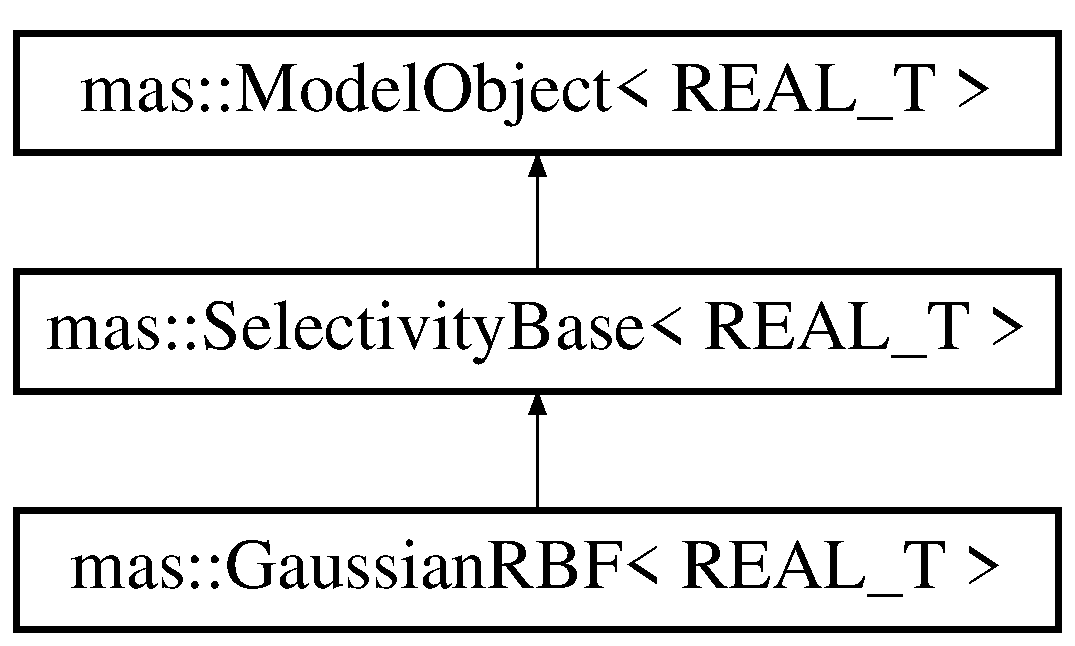
\includegraphics[height=3.000000cm]{structmas_1_1_gaussian_r_b_f}
\end{center}
\end{figure}
\subsection*{Public Types}
\begin{DoxyCompactItemize}
\item 
typedef \hyperlink{structmas_1_1_variable_trait}{Variable\-Trait}$<$ R\-E\-A\-L\-\_\-\-T $>$\\*
\-::\hyperlink{structmas_1_1_gaussian_r_b_f_a6aa7c2aa04e8a70a63c751cf240b37ab}{variable} \hyperlink{structmas_1_1_gaussian_r_b_f_a6aa7c2aa04e8a70a63c751cf240b37ab}{variable}
\end{DoxyCompactItemize}
\subsection*{Public Member Functions}
\begin{DoxyCompactItemize}
\item 
const \hyperlink{structmas_1_1_gaussian_r_b_f_a6aa7c2aa04e8a70a63c751cf240b37ab}{variable} \hyperlink{structmas_1_1_gaussian_r_b_f_add49065f4c597720e164588d5eece123}{Distance} (const \hyperlink{structmas_1_1_gaussian_r_b_f_a6aa7c2aa04e8a70a63c751cf240b37ab}{variable} \&a)
\item 
virtual const \hyperlink{structmas_1_1_gaussian_r_b_f_a6aa7c2aa04e8a70a63c751cf240b37ab}{variable} \hyperlink{structmas_1_1_gaussian_r_b_f_a29fededb3644678ef80d7c65f601dfae}{Evaluate} (const \hyperlink{structmas_1_1_gaussian_r_b_f_a6aa7c2aa04e8a70a63c751cf240b37ab}{variable} \&a)
\item 
virtual const \hyperlink{structmas_1_1_gaussian_r_b_f_a6aa7c2aa04e8a70a63c751cf240b37ab}{variable} \hyperlink{structmas_1_1_gaussian_r_b_f_a7710758db50657d20d5baf403713df87}{Evaluate} (const std\-::vector$<$ \hyperlink{structmas_1_1_gaussian_r_b_f_a6aa7c2aa04e8a70a63c751cf240b37ab}{variable} $>$ \&ages, size\-\_\-t index)
\item 
virtual const std\-::string \hyperlink{structmas_1_1_gaussian_r_b_f_a0b07e709655b2c7da7c89dd48491d091}{To\-J\-S\-O\-N\-String} ()
\item 
virtual const std\-::string \hyperlink{structmas_1_1_gaussian_r_b_f_a41b0813587b13d6b62dc5eedac91cc93}{Name} ()
\item 
virtual std\-::string \hyperlink{structmas_1_1_gaussian_r_b_f_a08856503cb0e77c17f891621aef50d21}{To\-String} ()
\end{DoxyCompactItemize}
\subsection*{Public Attributes}
\begin{DoxyCompactItemize}
\item 
\hyperlink{structmas_1_1_gaussian_r_b_f_a6aa7c2aa04e8a70a63c751cf240b37ab}{variable} \hyperlink{structmas_1_1_gaussian_r_b_f_ac42ac2ea9ca3bcb5c648f9829c34ee45}{centroid} = 1.\-1
\item 
\hyperlink{structmas_1_1_gaussian_r_b_f_a6aa7c2aa04e8a70a63c751cf240b37ab}{variable} \hyperlink{structmas_1_1_gaussian_r_b_f_a77f2e2c11d1166255d43e81853bc21a3}{epsilon} = 1.\-0
\item 
std\-::vector$<$ \hyperlink{structmas_1_1_gaussian_r_b_f_a6aa7c2aa04e8a70a63c751cf240b37ab}{variable} $>$ \hyperlink{structmas_1_1_gaussian_r_b_f_a47643c5b8933dfaa3c501effbf190639}{w}
\end{DoxyCompactItemize}


\subsection{Detailed Description}
\subsubsection*{template$<$typename R\-E\-A\-L\-\_\-\-T$>$struct mas\-::\-Gaussian\-R\-B\-F$<$ R\-E\-A\-L\-\_\-\-T $>$}

Age based logistic selectivity 
\begin{DoxyParams}{Parameters}
{\em a} & -\/ age \\
\hline
\end{DoxyParams}
\begin{DoxyReturn}{Returns}

\end{DoxyReturn}


Definition at line 189 of file Selectivity.\-hpp.



\subsection{Member Typedef Documentation}
\hypertarget{structmas_1_1_gaussian_r_b_f_a6aa7c2aa04e8a70a63c751cf240b37ab}{\index{mas\-::\-Gaussian\-R\-B\-F@{mas\-::\-Gaussian\-R\-B\-F}!variable@{variable}}
\index{variable@{variable}!mas::GaussianRBF@{mas\-::\-Gaussian\-R\-B\-F}}
\subsubsection[{variable}]{\setlength{\rightskip}{0pt plus 5cm}template$<$typename R\-E\-A\-L\-\_\-\-T $>$ typedef {\bf Variable\-Trait}$<$R\-E\-A\-L\-\_\-\-T$>$\-::{\bf variable} {\bf mas\-::\-Gaussian\-R\-B\-F}$<$ R\-E\-A\-L\-\_\-\-T $>$\-::{\bf variable}}}\label{structmas_1_1_gaussian_r_b_f_a6aa7c2aa04e8a70a63c751cf240b37ab}


Definition at line 190 of file Selectivity.\-hpp.



\subsection{Member Function Documentation}
\hypertarget{structmas_1_1_gaussian_r_b_f_add49065f4c597720e164588d5eece123}{\index{mas\-::\-Gaussian\-R\-B\-F@{mas\-::\-Gaussian\-R\-B\-F}!Distance@{Distance}}
\index{Distance@{Distance}!mas::GaussianRBF@{mas\-::\-Gaussian\-R\-B\-F}}
\subsubsection[{Distance}]{\setlength{\rightskip}{0pt plus 5cm}template$<$typename R\-E\-A\-L\-\_\-\-T $>$ const {\bf variable} {\bf mas\-::\-Gaussian\-R\-B\-F}$<$ R\-E\-A\-L\-\_\-\-T $>$\-::Distance (
\begin{DoxyParamCaption}
\item[{const {\bf variable} \&}]{a}
\end{DoxyParamCaption}
)\hspace{0.3cm}{\ttfamily [inline]}}}\label{structmas_1_1_gaussian_r_b_f_add49065f4c597720e164588d5eece123}


Definition at line 195 of file Selectivity.\-hpp.

\hypertarget{structmas_1_1_gaussian_r_b_f_a29fededb3644678ef80d7c65f601dfae}{\index{mas\-::\-Gaussian\-R\-B\-F@{mas\-::\-Gaussian\-R\-B\-F}!Evaluate@{Evaluate}}
\index{Evaluate@{Evaluate}!mas::GaussianRBF@{mas\-::\-Gaussian\-R\-B\-F}}
\subsubsection[{Evaluate}]{\setlength{\rightskip}{0pt plus 5cm}template$<$typename R\-E\-A\-L\-\_\-\-T $>$ virtual const {\bf variable} {\bf mas\-::\-Gaussian\-R\-B\-F}$<$ R\-E\-A\-L\-\_\-\-T $>$\-::Evaluate (
\begin{DoxyParamCaption}
\item[{const {\bf variable} \&}]{a}
\end{DoxyParamCaption}
)\hspace{0.3cm}{\ttfamily [inline]}, {\ttfamily [virtual]}}}\label{structmas_1_1_gaussian_r_b_f_a29fededb3644678ef80d7c65f601dfae}
Age based gaussian rbf selectivity 
\begin{DoxyParams}{Parameters}
{\em a} & -\/ age \\
\hline
\end{DoxyParams}
\begin{DoxyReturn}{Returns}

\end{DoxyReturn}


Implements \hyperlink{structmas_1_1_selectivity_base_a1c26fb2107d380ac4540271280031bf4}{mas\-::\-Selectivity\-Base$<$ R\-E\-A\-L\-\_\-\-T $>$}.



Definition at line 204 of file Selectivity.\-hpp.

\hypertarget{structmas_1_1_gaussian_r_b_f_a7710758db50657d20d5baf403713df87}{\index{mas\-::\-Gaussian\-R\-B\-F@{mas\-::\-Gaussian\-R\-B\-F}!Evaluate@{Evaluate}}
\index{Evaluate@{Evaluate}!mas::GaussianRBF@{mas\-::\-Gaussian\-R\-B\-F}}
\subsubsection[{Evaluate}]{\setlength{\rightskip}{0pt plus 5cm}template$<$typename R\-E\-A\-L\-\_\-\-T $>$ virtual const {\bf variable} {\bf mas\-::\-Gaussian\-R\-B\-F}$<$ R\-E\-A\-L\-\_\-\-T $>$\-::Evaluate (
\begin{DoxyParamCaption}
\item[{const std\-::vector$<$ {\bf variable} $>$ \&}]{ages, }
\item[{size\-\_\-t}]{index}
\end{DoxyParamCaption}
)\hspace{0.3cm}{\ttfamily [inline]}, {\ttfamily [virtual]}}}\label{structmas_1_1_gaussian_r_b_f_a7710758db50657d20d5baf403713df87}


Implements \hyperlink{structmas_1_1_selectivity_base_a52058fc9fe373bcc6deebd43bfc3f402}{mas\-::\-Selectivity\-Base$<$ R\-E\-A\-L\-\_\-\-T $>$}.



Definition at line 208 of file Selectivity.\-hpp.

\hypertarget{structmas_1_1_gaussian_r_b_f_a41b0813587b13d6b62dc5eedac91cc93}{\index{mas\-::\-Gaussian\-R\-B\-F@{mas\-::\-Gaussian\-R\-B\-F}!Name@{Name}}
\index{Name@{Name}!mas::GaussianRBF@{mas\-::\-Gaussian\-R\-B\-F}}
\subsubsection[{Name}]{\setlength{\rightskip}{0pt plus 5cm}template$<$typename R\-E\-A\-L\-\_\-\-T $>$ virtual const std\-::string {\bf mas\-::\-Gaussian\-R\-B\-F}$<$ R\-E\-A\-L\-\_\-\-T $>$\-::Name (
\begin{DoxyParamCaption}
{}
\end{DoxyParamCaption}
)\hspace{0.3cm}{\ttfamily [inline]}, {\ttfamily [virtual]}}}\label{structmas_1_1_gaussian_r_b_f_a41b0813587b13d6b62dc5eedac91cc93}


Reimplemented from \hyperlink{structmas_1_1_selectivity_base_ad14deefa4cddcc1c93ef17cc0a3e566a}{mas\-::\-Selectivity\-Base$<$ R\-E\-A\-L\-\_\-\-T $>$}.



Definition at line 232 of file Selectivity.\-hpp.

\hypertarget{structmas_1_1_gaussian_r_b_f_a0b07e709655b2c7da7c89dd48491d091}{\index{mas\-::\-Gaussian\-R\-B\-F@{mas\-::\-Gaussian\-R\-B\-F}!To\-J\-S\-O\-N\-String@{To\-J\-S\-O\-N\-String}}
\index{To\-J\-S\-O\-N\-String@{To\-J\-S\-O\-N\-String}!mas::GaussianRBF@{mas\-::\-Gaussian\-R\-B\-F}}
\subsubsection[{To\-J\-S\-O\-N\-String}]{\setlength{\rightskip}{0pt plus 5cm}template$<$typename R\-E\-A\-L\-\_\-\-T $>$ virtual const std\-::string {\bf mas\-::\-Gaussian\-R\-B\-F}$<$ R\-E\-A\-L\-\_\-\-T $>$\-::To\-J\-S\-O\-N\-String (
\begin{DoxyParamCaption}
{}
\end{DoxyParamCaption}
)\hspace{0.3cm}{\ttfamily [inline]}, {\ttfamily [virtual]}}}\label{structmas_1_1_gaussian_r_b_f_a0b07e709655b2c7da7c89dd48491d091}


Reimplemented from \hyperlink{structmas_1_1_model_object_af40b3c89b11919fc5aea21dcf1cd027b}{mas\-::\-Model\-Object$<$ R\-E\-A\-L\-\_\-\-T $>$}.



Definition at line 220 of file Selectivity.\-hpp.

\hypertarget{structmas_1_1_gaussian_r_b_f_a08856503cb0e77c17f891621aef50d21}{\index{mas\-::\-Gaussian\-R\-B\-F@{mas\-::\-Gaussian\-R\-B\-F}!To\-String@{To\-String}}
\index{To\-String@{To\-String}!mas::GaussianRBF@{mas\-::\-Gaussian\-R\-B\-F}}
\subsubsection[{To\-String}]{\setlength{\rightskip}{0pt plus 5cm}template$<$typename R\-E\-A\-L\-\_\-\-T $>$ virtual std\-::string {\bf mas\-::\-Gaussian\-R\-B\-F}$<$ R\-E\-A\-L\-\_\-\-T $>$\-::To\-String (
\begin{DoxyParamCaption}
{}
\end{DoxyParamCaption}
)\hspace{0.3cm}{\ttfamily [inline]}, {\ttfamily [virtual]}}}\label{structmas_1_1_gaussian_r_b_f_a08856503cb0e77c17f891621aef50d21}


Reimplemented from \hyperlink{structmas_1_1_model_object_a8eaf6c7c52e42ea8869aefa318358cb5}{mas\-::\-Model\-Object$<$ R\-E\-A\-L\-\_\-\-T $>$}.



Definition at line 236 of file Selectivity.\-hpp.



\subsection{Member Data Documentation}
\hypertarget{structmas_1_1_gaussian_r_b_f_ac42ac2ea9ca3bcb5c648f9829c34ee45}{\index{mas\-::\-Gaussian\-R\-B\-F@{mas\-::\-Gaussian\-R\-B\-F}!centroid@{centroid}}
\index{centroid@{centroid}!mas::GaussianRBF@{mas\-::\-Gaussian\-R\-B\-F}}
\subsubsection[{centroid}]{\setlength{\rightskip}{0pt plus 5cm}template$<$typename R\-E\-A\-L\-\_\-\-T $>$ {\bf variable} {\bf mas\-::\-Gaussian\-R\-B\-F}$<$ R\-E\-A\-L\-\_\-\-T $>$\-::centroid = 1.\-1}}\label{structmas_1_1_gaussian_r_b_f_ac42ac2ea9ca3bcb5c648f9829c34ee45}


Definition at line 191 of file Selectivity.\-hpp.

\hypertarget{structmas_1_1_gaussian_r_b_f_a77f2e2c11d1166255d43e81853bc21a3}{\index{mas\-::\-Gaussian\-R\-B\-F@{mas\-::\-Gaussian\-R\-B\-F}!epsilon@{epsilon}}
\index{epsilon@{epsilon}!mas::GaussianRBF@{mas\-::\-Gaussian\-R\-B\-F}}
\subsubsection[{epsilon}]{\setlength{\rightskip}{0pt plus 5cm}template$<$typename R\-E\-A\-L\-\_\-\-T $>$ {\bf variable} {\bf mas\-::\-Gaussian\-R\-B\-F}$<$ R\-E\-A\-L\-\_\-\-T $>$\-::epsilon = 1.\-0}}\label{structmas_1_1_gaussian_r_b_f_a77f2e2c11d1166255d43e81853bc21a3}


Definition at line 192 of file Selectivity.\-hpp.

\hypertarget{structmas_1_1_gaussian_r_b_f_a47643c5b8933dfaa3c501effbf190639}{\index{mas\-::\-Gaussian\-R\-B\-F@{mas\-::\-Gaussian\-R\-B\-F}!w@{w}}
\index{w@{w}!mas::GaussianRBF@{mas\-::\-Gaussian\-R\-B\-F}}
\subsubsection[{w}]{\setlength{\rightskip}{0pt plus 5cm}template$<$typename R\-E\-A\-L\-\_\-\-T $>$ std\-::vector$<${\bf variable}$>$ {\bf mas\-::\-Gaussian\-R\-B\-F}$<$ R\-E\-A\-L\-\_\-\-T $>$\-::w}}\label{structmas_1_1_gaussian_r_b_f_a47643c5b8933dfaa3c501effbf190639}


Definition at line 193 of file Selectivity.\-hpp.



The documentation for this struct was generated from the following file\-:\begin{DoxyCompactItemize}
\item 
/home/oppy/\-Net\-Beans\-Projects/mas/\hyperlink{_selectivity_8hpp}{Selectivity.\-hpp}\end{DoxyCompactItemize}

\hypertarget{structmas_1_1_growth_base}{\section{mas\-:\-:Growth\-Base$<$ R\-E\-A\-L\-\_\-\-T $>$ Struct Template Reference}
\label{structmas_1_1_growth_base}\index{mas\-::\-Growth\-Base$<$ R\-E\-A\-L\-\_\-\-T $>$@{mas\-::\-Growth\-Base$<$ R\-E\-A\-L\-\_\-\-T $>$}}
}


{\ttfamily \#include $<$Growth.\-hpp$>$}

Inheritance diagram for mas\-:\-:Growth\-Base$<$ R\-E\-A\-L\-\_\-\-T $>$\-:\begin{figure}[H]
\begin{center}
\leavevmode
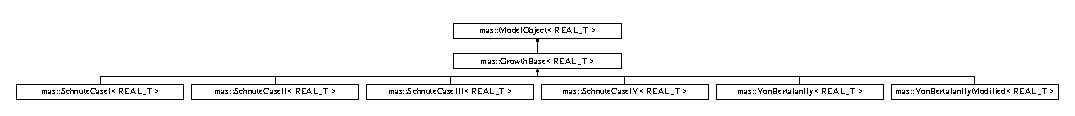
\includegraphics[height=1.111111cm]{structmas_1_1_growth_base}
\end{center}
\end{figure}
\subsection*{Public Types}
\begin{DoxyCompactItemize}
\item 
typedef \hyperlink{structmas_1_1_variable_trait}{Variable\-Trait}$<$ R\-E\-A\-L\-\_\-\-T $>$\\*
\-::\hyperlink{structmas_1_1_growth_base_a2b2f3559be1ce3134ab0a145fa3a8f43}{variable} \hyperlink{structmas_1_1_growth_base_a2b2f3559be1ce3134ab0a145fa3a8f43}{variable}
\end{DoxyCompactItemize}
\subsection*{Public Member Functions}
\begin{DoxyCompactItemize}
\item 
virtual const \hyperlink{structmas_1_1_growth_base_a2b2f3559be1ce3134ab0a145fa3a8f43}{variable} \hyperlink{structmas_1_1_growth_base_a381e3400e22b2739830351acdf4689b5}{Evaluate} (const \hyperlink{structmas_1_1_growth_base_a2b2f3559be1ce3134ab0a145fa3a8f43}{variable} \&age, const int \&sex)=0
\item 
const \hyperlink{structmas_1_1_growth_base_a2b2f3559be1ce3134ab0a145fa3a8f43}{variable} \hyperlink{structmas_1_1_growth_base_afa288d34bcad493a5a893ffe8d3c0920}{Weight} (const \hyperlink{structmas_1_1_growth_base_a2b2f3559be1ce3134ab0a145fa3a8f43}{variable} \&length, const int \&sex)
\item 
virtual const \hyperlink{structmas_1_1_growth_base_a2b2f3559be1ce3134ab0a145fa3a8f43}{variable} \hyperlink{structmas_1_1_growth_base_a74588899b86934b281e51b8a4fb15876}{Variance} (const \hyperlink{structmas_1_1_growth_base_a2b2f3559be1ce3134ab0a145fa3a8f43}{variable} \&age, const int \&sex)
\item 
virtual const std\-::string \hyperlink{structmas_1_1_growth_base_a3645c79a5cd9ed606bcf2f381aef5259}{Name} ()
\end{DoxyCompactItemize}
\subsection*{Public Attributes}
\begin{DoxyCompactItemize}
\item 
\hyperlink{structmas_1_1_growth_base_a2b2f3559be1ce3134ab0a145fa3a8f43}{variable} \hyperlink{structmas_1_1_growth_base_aab84c98377a8d04e4dcaaa7e7e19d2e2}{a\-\_\-min}
\item 
\hyperlink{structmas_1_1_growth_base_a2b2f3559be1ce3134ab0a145fa3a8f43}{variable} \hyperlink{structmas_1_1_growth_base_af5003b2a605a0107482b9dd9d368ef2d}{a\-\_\-max}
\item 
\hyperlink{structmas_1_1_growth_base_a2b2f3559be1ce3134ab0a145fa3a8f43}{variable} \hyperlink{structmas_1_1_growth_base_a412552f9b7d23d1c1f056e826b8981ae}{alpha\-\_\-f} = 0.\-000025
\item 
\hyperlink{structmas_1_1_growth_base_a2b2f3559be1ce3134ab0a145fa3a8f43}{variable} \hyperlink{structmas_1_1_growth_base_a396354505138367e93a446571e934e9e}{alpha\-\_\-m} = 0.\-000025
\item 
\hyperlink{structmas_1_1_growth_base_a2b2f3559be1ce3134ab0a145fa3a8f43}{variable} \hyperlink{structmas_1_1_growth_base_ab24d4baacfb805e7b48db9b74e332658}{beta\-\_\-f} = 3.\-0
\item 
\hyperlink{structmas_1_1_growth_base_a2b2f3559be1ce3134ab0a145fa3a8f43}{variable} \hyperlink{structmas_1_1_growth_base_a17b3c2eef24ac82f2feb94119eb4ae64}{beta\-\_\-m} = 3.\-0
\item 
std\-::shared\-\_\-ptr\\*
$<$ \hyperlink{structmas_1_1_data_object}{mas\-::\-Data\-Object}$<$ \hyperlink{structmas_1_1_growth_base_a2b2f3559be1ce3134ab0a145fa3a8f43}{variable} $>$ $>$ \hyperlink{structmas_1_1_growth_base_a8b31d8d43f6ec3383d3be31a674f997a}{age\-\_\-length\-\_\-key}
\end{DoxyCompactItemize}


\subsection{Detailed Description}
\subsubsection*{template$<$typename R\-E\-A\-L\-\_\-\-T$>$struct mas\-::\-Growth\-Base$<$ R\-E\-A\-L\-\_\-\-T $>$}



Definition at line 41 of file Growth.\-hpp.



\subsection{Member Typedef Documentation}
\hypertarget{structmas_1_1_growth_base_a2b2f3559be1ce3134ab0a145fa3a8f43}{\index{mas\-::\-Growth\-Base@{mas\-::\-Growth\-Base}!variable@{variable}}
\index{variable@{variable}!mas::GrowthBase@{mas\-::\-Growth\-Base}}
\subsubsection[{variable}]{\setlength{\rightskip}{0pt plus 5cm}template$<$typename R\-E\-A\-L\-\_\-\-T $>$ typedef {\bf Variable\-Trait}$<$R\-E\-A\-L\-\_\-\-T$>$\-::{\bf variable} {\bf mas\-::\-Growth\-Base}$<$ R\-E\-A\-L\-\_\-\-T $>$\-::{\bf variable}}}\label{structmas_1_1_growth_base_a2b2f3559be1ce3134ab0a145fa3a8f43}


Definition at line 42 of file Growth.\-hpp.



\subsection{Member Function Documentation}
\hypertarget{structmas_1_1_growth_base_a381e3400e22b2739830351acdf4689b5}{\index{mas\-::\-Growth\-Base@{mas\-::\-Growth\-Base}!Evaluate@{Evaluate}}
\index{Evaluate@{Evaluate}!mas::GrowthBase@{mas\-::\-Growth\-Base}}
\subsubsection[{Evaluate}]{\setlength{\rightskip}{0pt plus 5cm}template$<$typename R\-E\-A\-L\-\_\-\-T $>$ virtual const {\bf variable} {\bf mas\-::\-Growth\-Base}$<$ R\-E\-A\-L\-\_\-\-T $>$\-::Evaluate (
\begin{DoxyParamCaption}
\item[{const {\bf variable} \&}]{age, }
\item[{const int \&}]{sex}
\end{DoxyParamCaption}
)\hspace{0.3cm}{\ttfamily [pure virtual]}}}\label{structmas_1_1_growth_base_a381e3400e22b2739830351acdf4689b5}
Computes the length of a fish at age by sex.


\begin{DoxyParams}{Parameters}
{\em age} & \\
\hline
{\em sex} & \\
\hline
\end{DoxyParams}
\begin{DoxyReturn}{Returns}
length 
\end{DoxyReturn}


Implemented in \hyperlink{structmas_1_1_schnute_case_i_v_a8100c63161dead550bf517365e355fec}{mas\-::\-Schnute\-Case\-I\-V$<$ R\-E\-A\-L\-\_\-\-T $>$}, \hyperlink{structmas_1_1_schnute_case_i_i_i_a36829dacc125f07c7c9595f1e8ca0d8a}{mas\-::\-Schnute\-Case\-I\-I\-I$<$ R\-E\-A\-L\-\_\-\-T $>$}, \hyperlink{structmas_1_1_schnute_case_i_i_ac582befc654cf955f0afafed8889b0e1}{mas\-::\-Schnute\-Case\-I\-I$<$ R\-E\-A\-L\-\_\-\-T $>$}, \hyperlink{structmas_1_1_schnute_case_i_acc1a2f969120393ef5275ee3f297dfc9}{mas\-::\-Schnute\-Case\-I$<$ R\-E\-A\-L\-\_\-\-T $>$}, \hyperlink{structmas_1_1_von_bertalanffy_modified_ac5e51a32119b7353bb32d64f440416c7}{mas\-::\-Von\-Bertalanffy\-Modified$<$ R\-E\-A\-L\-\_\-\-T $>$}, and \hyperlink{structmas_1_1_von_bertalanffy_ac89c031af93f2baf47d357bca9c37b6a}{mas\-::\-Von\-Bertalanffy$<$ R\-E\-A\-L\-\_\-\-T $>$}.

\hypertarget{structmas_1_1_growth_base_a3645c79a5cd9ed606bcf2f381aef5259}{\index{mas\-::\-Growth\-Base@{mas\-::\-Growth\-Base}!Name@{Name}}
\index{Name@{Name}!mas::GrowthBase@{mas\-::\-Growth\-Base}}
\subsubsection[{Name}]{\setlength{\rightskip}{0pt plus 5cm}template$<$typename R\-E\-A\-L\-\_\-\-T $>$ virtual const std\-::string {\bf mas\-::\-Growth\-Base}$<$ R\-E\-A\-L\-\_\-\-T $>$\-::Name (
\begin{DoxyParamCaption}
{}
\end{DoxyParamCaption}
)\hspace{0.3cm}{\ttfamily [inline]}, {\ttfamily [virtual]}}}\label{structmas_1_1_growth_base_a3645c79a5cd9ed606bcf2f381aef5259}


Reimplemented in \hyperlink{structmas_1_1_schnute_case_i_v_a7193145ce124fd855fc7d950a936fc20}{mas\-::\-Schnute\-Case\-I\-V$<$ R\-E\-A\-L\-\_\-\-T $>$}, \hyperlink{structmas_1_1_schnute_case_i_i_i_a0b7e35620fbbdc033702c304054aa9e3}{mas\-::\-Schnute\-Case\-I\-I\-I$<$ R\-E\-A\-L\-\_\-\-T $>$}, \hyperlink{structmas_1_1_schnute_case_i_i_a1f2900afe54ea24bcd555dd5eab8ce03}{mas\-::\-Schnute\-Case\-I\-I$<$ R\-E\-A\-L\-\_\-\-T $>$}, \hyperlink{structmas_1_1_schnute_case_i_a5588227ee2b536f92b34c02d95a7d148}{mas\-::\-Schnute\-Case\-I$<$ R\-E\-A\-L\-\_\-\-T $>$}, \hyperlink{structmas_1_1_von_bertalanffy_modified_a6c845df6e13d5219cd56614d323aaa79}{mas\-::\-Von\-Bertalanffy\-Modified$<$ R\-E\-A\-L\-\_\-\-T $>$}, and \hyperlink{structmas_1_1_von_bertalanffy_a8d8c204940577c3b4e515baae839c15d}{mas\-::\-Von\-Bertalanffy$<$ R\-E\-A\-L\-\_\-\-T $>$}.



Definition at line 71 of file Growth.\-hpp.

\hypertarget{structmas_1_1_growth_base_a74588899b86934b281e51b8a4fb15876}{\index{mas\-::\-Growth\-Base@{mas\-::\-Growth\-Base}!Variance@{Variance}}
\index{Variance@{Variance}!mas::GrowthBase@{mas\-::\-Growth\-Base}}
\subsubsection[{Variance}]{\setlength{\rightskip}{0pt plus 5cm}template$<$typename R\-E\-A\-L\-\_\-\-T $>$ virtual const {\bf variable} {\bf mas\-::\-Growth\-Base}$<$ R\-E\-A\-L\-\_\-\-T $>$\-::Variance (
\begin{DoxyParamCaption}
\item[{const {\bf variable} \&}]{age, }
\item[{const int \&}]{sex}
\end{DoxyParamCaption}
)\hspace{0.3cm}{\ttfamily [inline]}, {\ttfamily [virtual]}}}\label{structmas_1_1_growth_base_a74588899b86934b281e51b8a4fb15876}


Definition at line 67 of file Growth.\-hpp.

\hypertarget{structmas_1_1_growth_base_afa288d34bcad493a5a893ffe8d3c0920}{\index{mas\-::\-Growth\-Base@{mas\-::\-Growth\-Base}!Weight@{Weight}}
\index{Weight@{Weight}!mas::GrowthBase@{mas\-::\-Growth\-Base}}
\subsubsection[{Weight}]{\setlength{\rightskip}{0pt plus 5cm}template$<$typename R\-E\-A\-L\-\_\-\-T $>$ const {\bf variable} {\bf mas\-::\-Growth\-Base}$<$ R\-E\-A\-L\-\_\-\-T $>$\-::Weight (
\begin{DoxyParamCaption}
\item[{const {\bf variable} \&}]{length, }
\item[{const int \&}]{sex}
\end{DoxyParamCaption}
)\hspace{0.3cm}{\ttfamily [inline]}}}\label{structmas_1_1_growth_base_afa288d34bcad493a5a893ffe8d3c0920}


Definition at line 62 of file Growth.\-hpp.



\subsection{Member Data Documentation}
\hypertarget{structmas_1_1_growth_base_af5003b2a605a0107482b9dd9d368ef2d}{\index{mas\-::\-Growth\-Base@{mas\-::\-Growth\-Base}!a\-\_\-max@{a\-\_\-max}}
\index{a\-\_\-max@{a\-\_\-max}!mas::GrowthBase@{mas\-::\-Growth\-Base}}
\subsubsection[{a\-\_\-max}]{\setlength{\rightskip}{0pt plus 5cm}template$<$typename R\-E\-A\-L\-\_\-\-T $>$ {\bf variable} {\bf mas\-::\-Growth\-Base}$<$ R\-E\-A\-L\-\_\-\-T $>$\-::a\-\_\-max}}\label{structmas_1_1_growth_base_af5003b2a605a0107482b9dd9d368ef2d}


Definition at line 44 of file Growth.\-hpp.

\hypertarget{structmas_1_1_growth_base_aab84c98377a8d04e4dcaaa7e7e19d2e2}{\index{mas\-::\-Growth\-Base@{mas\-::\-Growth\-Base}!a\-\_\-min@{a\-\_\-min}}
\index{a\-\_\-min@{a\-\_\-min}!mas::GrowthBase@{mas\-::\-Growth\-Base}}
\subsubsection[{a\-\_\-min}]{\setlength{\rightskip}{0pt plus 5cm}template$<$typename R\-E\-A\-L\-\_\-\-T $>$ {\bf variable} {\bf mas\-::\-Growth\-Base}$<$ R\-E\-A\-L\-\_\-\-T $>$\-::a\-\_\-min}}\label{structmas_1_1_growth_base_aab84c98377a8d04e4dcaaa7e7e19d2e2}


Definition at line 43 of file Growth.\-hpp.

\hypertarget{structmas_1_1_growth_base_a8b31d8d43f6ec3383d3be31a674f997a}{\index{mas\-::\-Growth\-Base@{mas\-::\-Growth\-Base}!age\-\_\-length\-\_\-key@{age\-\_\-length\-\_\-key}}
\index{age\-\_\-length\-\_\-key@{age\-\_\-length\-\_\-key}!mas::GrowthBase@{mas\-::\-Growth\-Base}}
\subsubsection[{age\-\_\-length\-\_\-key}]{\setlength{\rightskip}{0pt plus 5cm}template$<$typename R\-E\-A\-L\-\_\-\-T $>$ std\-::shared\-\_\-ptr$<${\bf mas\-::\-Data\-Object}$<${\bf variable}$>$ $>$ {\bf mas\-::\-Growth\-Base}$<$ R\-E\-A\-L\-\_\-\-T $>$\-::age\-\_\-length\-\_\-key}}\label{structmas_1_1_growth_base_a8b31d8d43f6ec3383d3be31a674f997a}


Definition at line 51 of file Growth.\-hpp.

\hypertarget{structmas_1_1_growth_base_a412552f9b7d23d1c1f056e826b8981ae}{\index{mas\-::\-Growth\-Base@{mas\-::\-Growth\-Base}!alpha\-\_\-f@{alpha\-\_\-f}}
\index{alpha\-\_\-f@{alpha\-\_\-f}!mas::GrowthBase@{mas\-::\-Growth\-Base}}
\subsubsection[{alpha\-\_\-f}]{\setlength{\rightskip}{0pt plus 5cm}template$<$typename R\-E\-A\-L\-\_\-\-T $>$ {\bf variable} {\bf mas\-::\-Growth\-Base}$<$ R\-E\-A\-L\-\_\-\-T $>$\-::alpha\-\_\-f = 0.\-000025}}\label{structmas_1_1_growth_base_a412552f9b7d23d1c1f056e826b8981ae}


Definition at line 46 of file Growth.\-hpp.

\hypertarget{structmas_1_1_growth_base_a396354505138367e93a446571e934e9e}{\index{mas\-::\-Growth\-Base@{mas\-::\-Growth\-Base}!alpha\-\_\-m@{alpha\-\_\-m}}
\index{alpha\-\_\-m@{alpha\-\_\-m}!mas::GrowthBase@{mas\-::\-Growth\-Base}}
\subsubsection[{alpha\-\_\-m}]{\setlength{\rightskip}{0pt plus 5cm}template$<$typename R\-E\-A\-L\-\_\-\-T $>$ {\bf variable} {\bf mas\-::\-Growth\-Base}$<$ R\-E\-A\-L\-\_\-\-T $>$\-::alpha\-\_\-m = 0.\-000025}}\label{structmas_1_1_growth_base_a396354505138367e93a446571e934e9e}


Definition at line 47 of file Growth.\-hpp.

\hypertarget{structmas_1_1_growth_base_ab24d4baacfb805e7b48db9b74e332658}{\index{mas\-::\-Growth\-Base@{mas\-::\-Growth\-Base}!beta\-\_\-f@{beta\-\_\-f}}
\index{beta\-\_\-f@{beta\-\_\-f}!mas::GrowthBase@{mas\-::\-Growth\-Base}}
\subsubsection[{beta\-\_\-f}]{\setlength{\rightskip}{0pt plus 5cm}template$<$typename R\-E\-A\-L\-\_\-\-T $>$ {\bf variable} {\bf mas\-::\-Growth\-Base}$<$ R\-E\-A\-L\-\_\-\-T $>$\-::beta\-\_\-f = 3.\-0}}\label{structmas_1_1_growth_base_ab24d4baacfb805e7b48db9b74e332658}


Definition at line 48 of file Growth.\-hpp.

\hypertarget{structmas_1_1_growth_base_a17b3c2eef24ac82f2feb94119eb4ae64}{\index{mas\-::\-Growth\-Base@{mas\-::\-Growth\-Base}!beta\-\_\-m@{beta\-\_\-m}}
\index{beta\-\_\-m@{beta\-\_\-m}!mas::GrowthBase@{mas\-::\-Growth\-Base}}
\subsubsection[{beta\-\_\-m}]{\setlength{\rightskip}{0pt plus 5cm}template$<$typename R\-E\-A\-L\-\_\-\-T $>$ {\bf variable} {\bf mas\-::\-Growth\-Base}$<$ R\-E\-A\-L\-\_\-\-T $>$\-::beta\-\_\-m = 3.\-0}}\label{structmas_1_1_growth_base_a17b3c2eef24ac82f2feb94119eb4ae64}


Definition at line 49 of file Growth.\-hpp.



The documentation for this struct was generated from the following file\-:\begin{DoxyCompactItemize}
\item 
/home/oppy/\-Net\-Beans\-Projects/mas/\hyperlink{_growth_8hpp}{Growth.\-hpp}\end{DoxyCompactItemize}

\hypertarget{structmas_1_1_h_c_r_base}{\section{mas\-:\-:H\-C\-R\-Base$<$ R\-E\-A\-L\-\_\-\-T $>$ Struct Template Reference}
\label{structmas_1_1_h_c_r_base}\index{mas\-::\-H\-C\-R\-Base$<$ R\-E\-A\-L\-\_\-\-T $>$@{mas\-::\-H\-C\-R\-Base$<$ R\-E\-A\-L\-\_\-\-T $>$}}
}


{\ttfamily \#include $<$Harvest\-Control\-Rule.\-hpp$>$}

Inheritance diagram for mas\-:\-:H\-C\-R\-Base$<$ R\-E\-A\-L\-\_\-\-T $>$\-:\begin{figure}[H]
\begin{center}
\leavevmode
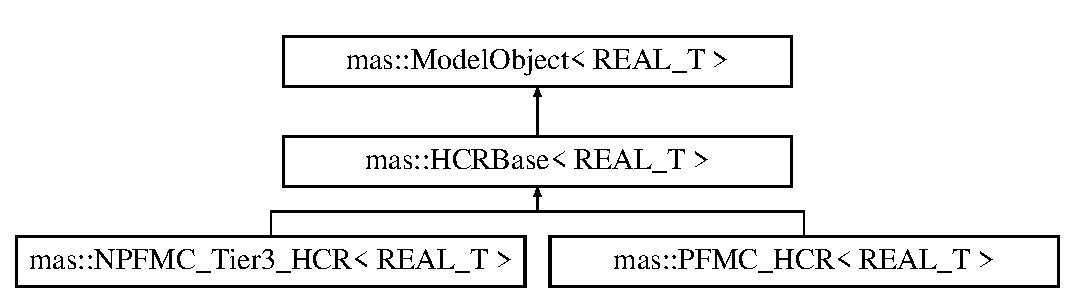
\includegraphics[height=3.000000cm]{structmas_1_1_h_c_r_base}
\end{center}
\end{figure}
\subsection*{Public Types}
\begin{DoxyCompactItemize}
\item 
typedef \hyperlink{structmas_1_1_variable_trait}{Variable\-Trait}$<$ R\-E\-A\-L\-\_\-\-T $>$\\*
\-::\hyperlink{structmas_1_1_model_object_a4e62fdbb5826f8fac311262b888ab10a}{variable} \hyperlink{structmas_1_1_h_c_r_base_a034a831895ed4a6c7224a1f7c4699c08}{variable}
\end{DoxyCompactItemize}
\subsection*{Public Member Functions}
\begin{DoxyCompactItemize}
\item 
virtual const std\-::tuple\\*
$<$ \hyperlink{structmas_1_1_model_object_a4e62fdbb5826f8fac311262b888ab10a}{variable}, \hyperlink{structmas_1_1_model_object_a4e62fdbb5826f8fac311262b888ab10a}{variable}, \hyperlink{structmas_1_1_model_object_a4e62fdbb5826f8fac311262b888ab10a}{variable}, \\*
\hyperlink{structmas_1_1_model_object_a4e62fdbb5826f8fac311262b888ab10a}{variable} $>$ \hyperlink{structmas_1_1_h_c_r_base_a3d923b3276f10e4c7938abde6a134291}{Evaluate} (const int \&year, const \hyperlink{structmas_1_1_area_population_info}{mas\-::\-Area\-Population\-Info}$<$ R\-E\-A\-L\-\_\-\-T $>$ \&api\-\_\-males, const \hyperlink{structmas_1_1_area_population_info}{mas\-::\-Area\-Population\-Info}$<$ R\-E\-A\-L\-\_\-\-T $>$ \&api\-\_\-females)=0
\item 
virtual const std\-::string \hyperlink{structmas_1_1_h_c_r_base_a3f1aa4335bee8d9225776ca5212e1085}{Name} ()
\end{DoxyCompactItemize}
\subsection*{Additional Inherited Members}


\subsection{Detailed Description}
\subsubsection*{template$<$typename R\-E\-A\-L\-\_\-\-T$>$struct mas\-::\-H\-C\-R\-Base$<$ R\-E\-A\-L\-\_\-\-T $>$}



Definition at line 50 of file Harvest\-Control\-Rule.\-hpp.



\subsection{Member Typedef Documentation}
\hypertarget{structmas_1_1_h_c_r_base_a034a831895ed4a6c7224a1f7c4699c08}{\index{mas\-::\-H\-C\-R\-Base@{mas\-::\-H\-C\-R\-Base}!variable@{variable}}
\index{variable@{variable}!mas::HCRBase@{mas\-::\-H\-C\-R\-Base}}
\subsubsection[{variable}]{\setlength{\rightskip}{0pt plus 5cm}template$<$typename R\-E\-A\-L\-\_\-\-T $>$ typedef {\bf Variable\-Trait}$<$R\-E\-A\-L\-\_\-\-T$>$\-::{\bf variable} {\bf mas\-::\-H\-C\-R\-Base}$<$ R\-E\-A\-L\-\_\-\-T $>$\-::{\bf variable}}}\label{structmas_1_1_h_c_r_base_a034a831895ed4a6c7224a1f7c4699c08}


Definition at line 52 of file Harvest\-Control\-Rule.\-hpp.



\subsection{Member Function Documentation}
\hypertarget{structmas_1_1_h_c_r_base_a3d923b3276f10e4c7938abde6a134291}{\index{mas\-::\-H\-C\-R\-Base@{mas\-::\-H\-C\-R\-Base}!Evaluate@{Evaluate}}
\index{Evaluate@{Evaluate}!mas::HCRBase@{mas\-::\-H\-C\-R\-Base}}
\subsubsection[{Evaluate}]{\setlength{\rightskip}{0pt plus 5cm}template$<$typename R\-E\-A\-L\-\_\-\-T $>$ virtual const std\-::tuple$<${\bf variable}, {\bf variable}, {\bf variable}, {\bf variable}$>$ {\bf mas\-::\-H\-C\-R\-Base}$<$ R\-E\-A\-L\-\_\-\-T $>$\-::Evaluate (
\begin{DoxyParamCaption}
\item[{const int \&}]{year, }
\item[{const {\bf mas\-::\-Area\-Population\-Info}$<$ R\-E\-A\-L\-\_\-\-T $>$ \&}]{api\-\_\-males, }
\item[{const {\bf mas\-::\-Area\-Population\-Info}$<$ R\-E\-A\-L\-\_\-\-T $>$ \&}]{api\-\_\-females}
\end{DoxyParamCaption}
)\hspace{0.3cm}{\ttfamily [pure virtual]}}}\label{structmas_1_1_h_c_r_base_a3d923b3276f10e4c7938abde6a134291}


Implemented in \hyperlink{structmas_1_1_p_f_m_c___h_c_r_a8e71e3c20bd5404dd350b9aca573a294}{mas\-::\-P\-F\-M\-C\-\_\-\-H\-C\-R$<$ R\-E\-A\-L\-\_\-\-T $>$}, and \hyperlink{structmas_1_1_n_p_f_m_c___tier3___h_c_r_af95105dd7d8a4a47ab028c34b35640ff}{mas\-::\-N\-P\-F\-M\-C\-\_\-\-Tier3\-\_\-\-H\-C\-R$<$ R\-E\-A\-L\-\_\-\-T $>$}.

\hypertarget{structmas_1_1_h_c_r_base_a3f1aa4335bee8d9225776ca5212e1085}{\index{mas\-::\-H\-C\-R\-Base@{mas\-::\-H\-C\-R\-Base}!Name@{Name}}
\index{Name@{Name}!mas::HCRBase@{mas\-::\-H\-C\-R\-Base}}
\subsubsection[{Name}]{\setlength{\rightskip}{0pt plus 5cm}template$<$typename R\-E\-A\-L\-\_\-\-T $>$ virtual const std\-::string {\bf mas\-::\-H\-C\-R\-Base}$<$ R\-E\-A\-L\-\_\-\-T $>$\-::Name (
\begin{DoxyParamCaption}
{}
\end{DoxyParamCaption}
)\hspace{0.3cm}{\ttfamily [inline]}, {\ttfamily [virtual]}}}\label{structmas_1_1_h_c_r_base_a3f1aa4335bee8d9225776ca5212e1085}


Reimplemented in \hyperlink{structmas_1_1_p_f_m_c___h_c_r_a5571d69b3043c8a56b92e96a4f1837b5}{mas\-::\-P\-F\-M\-C\-\_\-\-H\-C\-R$<$ R\-E\-A\-L\-\_\-\-T $>$}, and \hyperlink{structmas_1_1_n_p_f_m_c___tier3___h_c_r_a1f7d15c97821f987d8b8ef1a2c8099a5}{mas\-::\-N\-P\-F\-M\-C\-\_\-\-Tier3\-\_\-\-H\-C\-R$<$ R\-E\-A\-L\-\_\-\-T $>$}.



Definition at line 56 of file Harvest\-Control\-Rule.\-hpp.



The documentation for this struct was generated from the following file\-:\begin{DoxyCompactItemize}
\item 
/home/oppy/\-Net\-Beans\-Projects/mas/\hyperlink{_harvest_control_rule_8hpp}{Harvest\-Control\-Rule.\-hpp}\end{DoxyCompactItemize}

\hypertarget{classmas_1_1_information}{\section{mas\-:\-:Information$<$ R\-E\-A\-L\-\_\-\-T $>$ Class Template Reference}
\label{classmas_1_1_information}\index{mas\-::\-Information$<$ R\-E\-A\-L\-\_\-\-T $>$@{mas\-::\-Information$<$ R\-E\-A\-L\-\_\-\-T $>$}}
}


{\ttfamily \#include $<$Information.\-hpp$>$}

Inheritance diagram for mas\-:\-:Information$<$ R\-E\-A\-L\-\_\-\-T $>$\-:\begin{figure}[H]
\begin{center}
\leavevmode
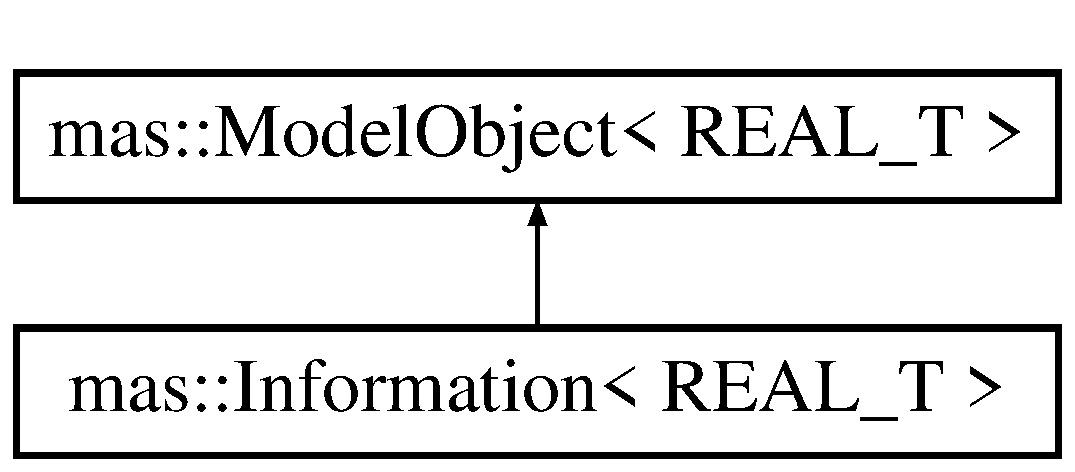
\includegraphics[height=2.000000cm]{classmas_1_1_information}
\end{center}
\end{figure}
\subsection*{Public Types}
\begin{DoxyCompactItemize}
\item 
typedef std\-::unordered\-\_\-map\\*
$<$ int, std\-::shared\-\_\-ptr\\*
$<$ \hyperlink{structmas_1_1_season}{mas\-::\-Season}$<$ R\-E\-A\-L\-\_\-\-T $>$\\*
 $>$ $>$\-::iterator \hyperlink{classmas_1_1_information_a4ada3467c12527ed5400cc67e80e31f2}{seasons\-\_\-iterator}
\item 
typedef std\-::unordered\-\_\-map\\*
$<$ int, std\-::shared\-\_\-ptr\\*
$<$ \hyperlink{structmas_1_1_area}{mas\-::\-Area}$<$ R\-E\-A\-L\-\_\-\-T $>$\\*
 $>$ $>$\-::iterator \hyperlink{classmas_1_1_information_a6183f0d8819e3ecb50239da88d2cfdb3}{area\-\_\-iterator}
\item 
typedef std\-::unordered\-\_\-map\\*
$<$ int, std\-::shared\-\_\-ptr\\*
$<$ \hyperlink{classmas_1_1_population}{mas\-::\-Population}$<$ R\-E\-A\-L\-\_\-\-T $>$\\*
 $>$ $>$\-::iterator \hyperlink{classmas_1_1_information_a61b09f185a136338d02e6307134677d1}{population\-\_\-iterator}
\item 
typedef std\-::unordered\-\_\-map\\*
$<$ int, std\-::shared\-\_\-ptr\\*
$<$ \hyperlink{structmas_1_1_growth_base}{mas\-::\-Growth\-Base}$<$ R\-E\-A\-L\-\_\-\-T $>$\\*
 $>$ $>$\-::iterator \hyperlink{classmas_1_1_information_aa19e91aec674c826cbb84ebdc1d17be7}{growth\-\_\-model\-\_\-iterator}
\item 
typedef std\-::unordered\-\_\-map\\*
$<$ int, std\-::shared\-\_\-ptr\\*
$<$ \hyperlink{structmas_1_1_recruitment_base}{mas\-::\-Recruitment\-Base}$<$ R\-E\-A\-L\-\_\-\-T $>$\\*
 $>$ $>$\-::iterator \hyperlink{classmas_1_1_information_a3948a990e86ca1174a515134fbd78dc5}{recruitment\-\_\-model\-\_\-iterator}
\item 
typedef std\-::unordered\-\_\-map\\*
$<$ int, std\-::shared\-\_\-ptr\\*
$<$ \hyperlink{structmas_1_1_natural_mortality}{mas\-::\-Natural\-Mortality}\\*
$<$ R\-E\-A\-L\-\_\-\-T $>$ $>$ $>$\-::iterator \hyperlink{classmas_1_1_information_a146940168f5079ca711b74f29ea7d6bc}{natural\-\_\-mortality\-\_\-model\-\_\-iterator}
\item 
typedef std\-::unordered\-\_\-map\\*
$<$ int, std\-::shared\-\_\-ptr\\*
$<$ \hyperlink{structmas_1_1_fishing_mortality}{mas\-::\-Fishing\-Mortality}\\*
$<$ R\-E\-A\-L\-\_\-\-T $>$ $>$ $>$\-::iterator \hyperlink{classmas_1_1_information_a4410f0f10156666ee305f22698943955}{fishing\-\_\-mortality\-\_\-model\-\_\-iterator}
\item 
typedef std\-::unordered\-\_\-map\\*
$<$ int, std\-::shared\-\_\-ptr\\*
$<$ \hyperlink{structmas_1_1_fecundity_base}{mas\-::\-Fecundity\-Base}$<$ R\-E\-A\-L\-\_\-\-T $>$\\*
 $>$ $>$\-::iterator \hyperlink{classmas_1_1_information_a1d4b59c5d61de9efed4709ce6e0a056a}{fecundity\-\_\-model\-\_\-iterator}
\item 
typedef std\-::unordered\-\_\-map\\*
$<$ int, std\-::shared\-\_\-ptr\\*
$<$ \hyperlink{structmas_1_1_movement}{mas\-::\-Movement}$<$ R\-E\-A\-L\-\_\-\-T $>$\\*
 $>$ $>$\-::iterator \hyperlink{classmas_1_1_information_aa69e662c74a82f02c72a94684c289490}{movement\-\_\-model\-\_\-iterator}
\item 
typedef std\-::unordered\-\_\-map\\*
$<$ int, std\-::shared\-\_\-ptr\\*
$<$ \hyperlink{structmas_1_1_selectivity_base}{mas\-::\-Selectivity\-Base}$<$ R\-E\-A\-L\-\_\-\-T $>$\\*
 $>$ $>$\-::iterator \hyperlink{classmas_1_1_information_a0760e4946119a28f018ff73cbdd0171f}{selectivity\-\_\-model\-\_\-iterator}
\item 
typedef std\-::unordered\-\_\-map\\*
$<$ int, std\-::shared\-\_\-ptr\\*
$<$ \hyperlink{structmas_1_1_fleet}{mas\-::\-Fleet}$<$ R\-E\-A\-L\-\_\-\-T $>$\\*
 $>$ $>$\-::iterator \hyperlink{classmas_1_1_information_a35add34ab4432f87d932531b06444ff7}{fleet\-\_\-iterator}
\item 
typedef std\-::unordered\-\_\-map\\*
$<$ int, std\-::shared\-\_\-ptr\\*
$<$ \hyperlink{structmas_1_1_survey}{mas\-::\-Survey}$<$ R\-E\-A\-L\-\_\-\-T $>$\\*
 $>$ $>$\-::iterator \hyperlink{classmas_1_1_information_ababaa75ccc01c68865bae68aa44453b3}{survey\-\_\-model\-\_\-iterator}
\item 
typedef std\-::unordered\-\_\-map\\*
$<$ int, std\-::shared\-\_\-ptr\\*
$<$ \hyperlink{structmas_1_1_n_l_l_functor}{mas\-::\-N\-L\-L\-Functor}$<$ R\-E\-A\-L\-\_\-\-T $>$\\*
 $>$ $>$\-::iterator \hyperlink{classmas_1_1_information_a566708cde6d1c6f4846f41566c6ee846}{likelihood\-\_\-components\-\_\-iterator}
\end{DoxyCompactItemize}
\subsection*{Public Member Functions}
\begin{DoxyCompactItemize}
\item 
\hyperlink{classmas_1_1_information_aff6ea69c6e89a795900043e3ee6b25b3}{Information} ()
\item 
\hyperlink{classmas_1_1_information_a01305102ef89867b1fbdc545c4af3893}{Information} (const \hyperlink{classmas_1_1_information}{Information}$<$ R\-E\-A\-L\-\_\-\-T $>$ \&orig)
\item 
virtual \hyperlink{classmas_1_1_information_a22f67a9193a45e1d7917e96e6f79bcb0}{$\sim$\-Information} ()
\item 
void \hyperlink{classmas_1_1_information_a87d31bf74b83b4d90cc49a6ce0830da5}{Write\-J\-S\-O\-N\-Config} (const std\-::string \&path)
\item 
void \hyperlink{classmas_1_1_information_a7637882f3b75458d88dee1075f2483f0}{Parse\-Config} (const std\-::string \&path)
\item 
void \hyperlink{classmas_1_1_information_aed7467a3ffe58e76ef6910f4f3dc1d95}{Handle\-Likelihood\-Component} (rapidjson\-::\-Document\-::\-Member\-Iterator \&likelihood\-\_\-component)
\item 
void \hyperlink{classmas_1_1_information_ace06cf6d7f8c2c65bcc5264fcdea7808}{Handle\-Survey\-Model} (rapidjson\-::\-Document\-::\-Member\-Iterator \&survey\-\_\-model)
\item 
void \hyperlink{classmas_1_1_information_a390e0c06f1dde7a6971fdc58bc3faa94}{Handle\-Fishing\-Mortality\-Model} (rapidjson\-::\-Document\-::\-Member\-Iterator \&mortality\-\_\-model)
\item 
void \hyperlink{classmas_1_1_information_ad07e1708a544dd3f31184793b1985136}{Handle\-Natural\-Mortality\-Model} (rapidjson\-::\-Document\-::\-Member\-Iterator \&mortality\-\_\-model)
\item 
void \hyperlink{classmas_1_1_information_a5f5c3c867caa0875099f7619842c4897}{Handle\-Movement\-Model} (rapidjson\-::\-Document\-::\-Member\-Iterator \&movement\-\_\-model)
\item 
void \hyperlink{classmas_1_1_information_aaf3678eaf754f85e15b713271b2ca29d}{Handle\-Fleet\-Model} (rapidjson\-::\-Document\-::\-Member\-Iterator \&fleet\-\_\-model)
\item 
void \hyperlink{classmas_1_1_information_a45a60ea2a7c1082e8f73da9822056afd}{Handle\-Population\-Model} (rapidjson\-::\-Document\-::\-Member\-Iterator \&population\-\_\-model)
\item 
void \hyperlink{classmas_1_1_information_a0a3b16dccc3c1e9c83791f9ee499e345}{Handle\-Area\-Model} (rapidjson\-::\-Document\-::\-Member\-Iterator \&area\-\_\-model)
\item 
void \hyperlink{classmas_1_1_information_a8b90279ef4aee66ac9d983f337350ffc}{Handle\-Selectivity\-Model} (rapidjson\-::\-Document\-::\-Member\-Iterator \&selectivity\-\_\-model)
\item 
void \hyperlink{classmas_1_1_information_a01ef7a80bb30104b29e2a02f8a68585b}{Handle\-Growth\-Model} (rapidjson\-::\-Document\-::\-Member\-Iterator \&growth\-\_\-model)
\item 
void \hyperlink{classmas_1_1_information_a7a1ada30329d94513bd1fe4da9f5eada}{Handle\-Recruitment\-Model} (rapidjson\-::\-Document\-::\-Member\-Iterator \&recruitment\-\_\-model)
\item 
void \hyperlink{classmas_1_1_information_aa9231a08baef815e554c9409721db949}{Parse\-Data} (const std\-::string \&path)
\item 
void \hyperlink{classmas_1_1_information_a4acd2cd593e38ff9811a8b82f8d80b9f}{Show\-Data} ()
\item 
void \hyperlink{classmas_1_1_information_aedf136f9e26677da4001be0246416ec9}{Create\-Model} ()
\item 
std\-::unordered\-\_\-map$<$ int, \\*
std\-::shared\-\_\-ptr\\*
$<$ \hyperlink{classmas_1_1_population}{mas\-::\-Population}$<$ R\-E\-A\-L\-\_\-\-T $>$ $>$ $>$ \& \hyperlink{classmas_1_1_information_a2f8b99cfb05913e795d8039fee851867}{Get\-Populations} ()
\item 
void \hyperlink{classmas_1_1_information_a5d48355043bf563672afdb6d2881eba6}{Dump\-Fishing\-Mortality} (std\-::string file)
\item 
void \hyperlink{classmas_1_1_information_a4507090a348f2fa3b5a1cb3a53138004}{Dump\-Selectivity} (std\-::string file)
\end{DoxyCompactItemize}
\subsection*{Public Attributes}
\begin{DoxyCompactItemize}
\item 
int \hyperlink{classmas_1_1_information_aba4d8ca8604985a74a51beb13dae9d55}{nyears}
\item 
int \hyperlink{classmas_1_1_information_a454f7c72980b885c8a3f52a651435dde}{nseasons} = 1
\item 
int \hyperlink{classmas_1_1_information_a7c6cdee59338bfc38ff3cc7a4d49cdd7}{first\-\_\-year}
\item 
int \hyperlink{classmas_1_1_information_ae988a6b80c30334b911f952df97201cc}{last\-\_\-year}
\item 
std\-::vector$<$ variable $>$ \hyperlink{classmas_1_1_information_a5522e2cd2f93a0ac42574f96acd9dbcd}{ages}
\item 
bool \hyperlink{classmas_1_1_information_abfd53a611fac22190c00882c84b8c39d}{natal\-\_\-movement} = false
\item 
bool \hyperlink{classmas_1_1_information_a5205ee6cc8165f1bf1feb30c6332fbb9}{valid\-\_\-configuration} = true
\item 
std\-::unordered\-\_\-map$<$ int, \\*
std\-::shared\-\_\-ptr$<$ \hyperlink{structmas_1_1_area}{mas\-::\-Area}\\*
$<$ R\-E\-A\-L\-\_\-\-T $>$ $>$ $>$ \hyperlink{classmas_1_1_information_a1d2b80f338f3a82fa8a85cfbac2c490d}{areas}
\item 
std\-::unordered\-\_\-map$<$ int, \\*
std\-::shared\-\_\-ptr$<$ \hyperlink{structmas_1_1_season}{mas\-::\-Season}\\*
$<$ R\-E\-A\-L\-\_\-\-T $>$ $>$ $>$ \hyperlink{classmas_1_1_information_a65c0643d2ab88f4e23004aaf9565b359}{seasons}
\item 
std\-::unordered\-\_\-map$<$ int, \\*
std\-::shared\-\_\-ptr\\*
$<$ \hyperlink{classmas_1_1_population}{mas\-::\-Population}$<$ R\-E\-A\-L\-\_\-\-T $>$ $>$ $>$ \hyperlink{classmas_1_1_information_aea96825c5714a43ad531811a402d8d39}{populations}
\item 
std\-::unordered\-\_\-map$<$ int, \\*
std\-::shared\-\_\-ptr\\*
$<$ \hyperlink{structmas_1_1_fishing_mortality}{mas\-::\-Fishing\-Mortality}\\*
$<$ R\-E\-A\-L\-\_\-\-T $>$ $>$ $>$ \hyperlink{classmas_1_1_information_a104fa47bf1c9f21b186059d4897f0dad}{fishing\-\_\-mortality\-\_\-models}
\item 
std\-::unordered\-\_\-map$<$ int, \\*
std\-::shared\-\_\-ptr\\*
$<$ \hyperlink{structmas_1_1_selectivity_base}{mas\-::\-Selectivity\-Base}$<$ R\-E\-A\-L\-\_\-\-T $>$ $>$ $>$ \hyperlink{classmas_1_1_information_ae771fa7c04d112e57d58ade01645d298}{selectivity\-\_\-models}
\item 
std\-::unordered\-\_\-map$<$ int, \\*
std\-::shared\-\_\-ptr$<$ \hyperlink{structmas_1_1_fleet}{mas\-::\-Fleet}\\*
$<$ R\-E\-A\-L\-\_\-\-T $>$ $>$ $>$ \hyperlink{classmas_1_1_information_a2790d8daab0d9435a246dd9823772500}{fleets}
\item 
std\-::unordered\-\_\-map$<$ int, \\*
std\-::shared\-\_\-ptr$<$ \hyperlink{structmas_1_1_survey}{mas\-::\-Survey}\\*
$<$ R\-E\-A\-L\-\_\-\-T $>$ $>$ $>$ \hyperlink{classmas_1_1_information_ad9eb1c49a6565f76e0605afdb39fa8fa}{survey\-\_\-models}
\item 
std\-::unordered\-\_\-map$<$ int, \\*
std\-::shared\-\_\-ptr\\*
$<$ \hyperlink{structmas_1_1_growth_base}{mas\-::\-Growth\-Base}$<$ R\-E\-A\-L\-\_\-\-T $>$ $>$ $>$ \hyperlink{classmas_1_1_information_a0088dd940274db906032cd1d91abdedc}{growth\-\_\-models}
\item 
std\-::unordered\-\_\-map$<$ int, \\*
std\-::shared\-\_\-ptr\\*
$<$ \hyperlink{structmas_1_1_fecundity_base}{mas\-::\-Fecundity\-Base}$<$ R\-E\-A\-L\-\_\-\-T $>$ $>$ $>$ \hyperlink{classmas_1_1_information_ac4ed9602f5cf956d2225e2cfc9ec84c1}{fecundity\-\_\-models}
\item 
std\-::unordered\-\_\-map$<$ int, \\*
std\-::shared\-\_\-ptr$<$ \hyperlink{structmas_1_1_movement}{mas\-::\-Movement}\\*
$<$ R\-E\-A\-L\-\_\-\-T $>$ $>$ $>$ \hyperlink{classmas_1_1_information_a0e3fd8c389a107440c7e5e57fe933527}{movement\-\_\-models}
\item 
std\-::unordered\-\_\-map$<$ int, \\*
std\-::shared\-\_\-ptr\\*
$<$ \hyperlink{structmas_1_1_natural_mortality}{mas\-::\-Natural\-Mortality}\\*
$<$ R\-E\-A\-L\-\_\-\-T $>$ $>$ $>$ \hyperlink{classmas_1_1_information_acf9c6846c98a230ec902d85e3ee3b5c8}{natural\-\_\-mortality\-\_\-models}
\item 
std\-::unordered\-\_\-map$<$ int, \\*
std\-::shared\-\_\-ptr\\*
$<$ \hyperlink{structmas_1_1_recruitment_base}{mas\-::\-Recruitment\-Base}$<$ R\-E\-A\-L\-\_\-\-T $>$ $>$ $>$ \hyperlink{classmas_1_1_information_ad540badf665ee856a5de0e4da0bb2e5e}{recruitment\-\_\-models}
\item 
std\-::unordered\-\_\-map$<$ int, \\*
std\-::shared\-\_\-ptr\\*
$<$ \hyperlink{structmas_1_1_n_l_l_functor}{mas\-::\-N\-L\-L\-Functor}$<$ R\-E\-A\-L\-\_\-\-T $>$ $>$ $>$ \hyperlink{classmas_1_1_information_aa58693a25eea57a0080bb4b99515fc23}{likelihood\-\_\-components}
\end{DoxyCompactItemize}


\subsection{Detailed Description}
\subsubsection*{template$<$typename R\-E\-A\-L\-\_\-\-T$>$class mas\-::\-Information$<$ R\-E\-A\-L\-\_\-\-T $>$}



Definition at line 63 of file Information.\-hpp.



\subsection{Member Typedef Documentation}
\hypertarget{classmas_1_1_information_a6183f0d8819e3ecb50239da88d2cfdb3}{\index{mas\-::\-Information@{mas\-::\-Information}!area\-\_\-iterator@{area\-\_\-iterator}}
\index{area\-\_\-iterator@{area\-\_\-iterator}!mas::Information@{mas\-::\-Information}}
\subsubsection[{area\-\_\-iterator}]{\setlength{\rightskip}{0pt plus 5cm}template$<$typename R\-E\-A\-L\-\_\-\-T$>$ typedef std\-::unordered\-\_\-map$<$int, std\-::shared\-\_\-ptr$<${\bf mas\-::\-Area}$<$R\-E\-A\-L\-\_\-\-T$>$ $>$ $>$\-::iterator {\bf mas\-::\-Information}$<$ R\-E\-A\-L\-\_\-\-T $>$\-::{\bf area\-\_\-iterator}}}\label{classmas_1_1_information_a6183f0d8819e3ecb50239da88d2cfdb3}


Definition at line 112 of file Information.\-hpp.

\hypertarget{classmas_1_1_information_a1d4b59c5d61de9efed4709ce6e0a056a}{\index{mas\-::\-Information@{mas\-::\-Information}!fecundity\-\_\-model\-\_\-iterator@{fecundity\-\_\-model\-\_\-iterator}}
\index{fecundity\-\_\-model\-\_\-iterator@{fecundity\-\_\-model\-\_\-iterator}!mas::Information@{mas\-::\-Information}}
\subsubsection[{fecundity\-\_\-model\-\_\-iterator}]{\setlength{\rightskip}{0pt plus 5cm}template$<$typename R\-E\-A\-L\-\_\-\-T$>$ typedef std\-::unordered\-\_\-map$<$int, std\-::shared\-\_\-ptr$<${\bf mas\-::\-Fecundity\-Base}$<$R\-E\-A\-L\-\_\-\-T$>$ $>$ $>$\-::iterator {\bf mas\-::\-Information}$<$ R\-E\-A\-L\-\_\-\-T $>$\-::{\bf fecundity\-\_\-model\-\_\-iterator}}}\label{classmas_1_1_information_a1d4b59c5d61de9efed4709ce6e0a056a}


Definition at line 118 of file Information.\-hpp.

\hypertarget{classmas_1_1_information_a4410f0f10156666ee305f22698943955}{\index{mas\-::\-Information@{mas\-::\-Information}!fishing\-\_\-mortality\-\_\-model\-\_\-iterator@{fishing\-\_\-mortality\-\_\-model\-\_\-iterator}}
\index{fishing\-\_\-mortality\-\_\-model\-\_\-iterator@{fishing\-\_\-mortality\-\_\-model\-\_\-iterator}!mas::Information@{mas\-::\-Information}}
\subsubsection[{fishing\-\_\-mortality\-\_\-model\-\_\-iterator}]{\setlength{\rightskip}{0pt plus 5cm}template$<$typename R\-E\-A\-L\-\_\-\-T$>$ typedef std\-::unordered\-\_\-map$<$int, std\-::shared\-\_\-ptr$<${\bf mas\-::\-Fishing\-Mortality}$<$R\-E\-A\-L\-\_\-\-T$>$ $>$ $>$\-::iterator {\bf mas\-::\-Information}$<$ R\-E\-A\-L\-\_\-\-T $>$\-::{\bf fishing\-\_\-mortality\-\_\-model\-\_\-iterator}}}\label{classmas_1_1_information_a4410f0f10156666ee305f22698943955}


Definition at line 117 of file Information.\-hpp.

\hypertarget{classmas_1_1_information_a35add34ab4432f87d932531b06444ff7}{\index{mas\-::\-Information@{mas\-::\-Information}!fleet\-\_\-iterator@{fleet\-\_\-iterator}}
\index{fleet\-\_\-iterator@{fleet\-\_\-iterator}!mas::Information@{mas\-::\-Information}}
\subsubsection[{fleet\-\_\-iterator}]{\setlength{\rightskip}{0pt plus 5cm}template$<$typename R\-E\-A\-L\-\_\-\-T$>$ typedef std\-::unordered\-\_\-map$<$int, std\-::shared\-\_\-ptr$<${\bf mas\-::\-Fleet}$<$R\-E\-A\-L\-\_\-\-T$>$ $>$ $>$\-::iterator {\bf mas\-::\-Information}$<$ R\-E\-A\-L\-\_\-\-T $>$\-::{\bf fleet\-\_\-iterator}}}\label{classmas_1_1_information_a35add34ab4432f87d932531b06444ff7}


Definition at line 121 of file Information.\-hpp.

\hypertarget{classmas_1_1_information_aa19e91aec674c826cbb84ebdc1d17be7}{\index{mas\-::\-Information@{mas\-::\-Information}!growth\-\_\-model\-\_\-iterator@{growth\-\_\-model\-\_\-iterator}}
\index{growth\-\_\-model\-\_\-iterator@{growth\-\_\-model\-\_\-iterator}!mas::Information@{mas\-::\-Information}}
\subsubsection[{growth\-\_\-model\-\_\-iterator}]{\setlength{\rightskip}{0pt plus 5cm}template$<$typename R\-E\-A\-L\-\_\-\-T$>$ typedef std\-::unordered\-\_\-map$<$int, std\-::shared\-\_\-ptr$<${\bf mas\-::\-Growth\-Base}$<$R\-E\-A\-L\-\_\-\-T$>$ $>$ $>$\-::iterator {\bf mas\-::\-Information}$<$ R\-E\-A\-L\-\_\-\-T $>$\-::{\bf growth\-\_\-model\-\_\-iterator}}}\label{classmas_1_1_information_aa19e91aec674c826cbb84ebdc1d17be7}


Definition at line 114 of file Information.\-hpp.

\hypertarget{classmas_1_1_information_a566708cde6d1c6f4846f41566c6ee846}{\index{mas\-::\-Information@{mas\-::\-Information}!likelihood\-\_\-components\-\_\-iterator@{likelihood\-\_\-components\-\_\-iterator}}
\index{likelihood\-\_\-components\-\_\-iterator@{likelihood\-\_\-components\-\_\-iterator}!mas::Information@{mas\-::\-Information}}
\subsubsection[{likelihood\-\_\-components\-\_\-iterator}]{\setlength{\rightskip}{0pt plus 5cm}template$<$typename R\-E\-A\-L\-\_\-\-T$>$ typedef std\-::unordered\-\_\-map$<$int, std\-::shared\-\_\-ptr$<${\bf mas\-::\-N\-L\-L\-Functor}$<$R\-E\-A\-L\-\_\-\-T$>$ $>$ $>$\-::iterator {\bf mas\-::\-Information}$<$ R\-E\-A\-L\-\_\-\-T $>$\-::{\bf likelihood\-\_\-components\-\_\-iterator}}}\label{classmas_1_1_information_a566708cde6d1c6f4846f41566c6ee846}


Definition at line 123 of file Information.\-hpp.

\hypertarget{classmas_1_1_information_aa69e662c74a82f02c72a94684c289490}{\index{mas\-::\-Information@{mas\-::\-Information}!movement\-\_\-model\-\_\-iterator@{movement\-\_\-model\-\_\-iterator}}
\index{movement\-\_\-model\-\_\-iterator@{movement\-\_\-model\-\_\-iterator}!mas::Information@{mas\-::\-Information}}
\subsubsection[{movement\-\_\-model\-\_\-iterator}]{\setlength{\rightskip}{0pt plus 5cm}template$<$typename R\-E\-A\-L\-\_\-\-T$>$ typedef std\-::unordered\-\_\-map$<$int, std\-::shared\-\_\-ptr$<${\bf mas\-::\-Movement}$<$R\-E\-A\-L\-\_\-\-T$>$ $>$ $>$\-::iterator {\bf mas\-::\-Information}$<$ R\-E\-A\-L\-\_\-\-T $>$\-::{\bf movement\-\_\-model\-\_\-iterator}}}\label{classmas_1_1_information_aa69e662c74a82f02c72a94684c289490}


Definition at line 119 of file Information.\-hpp.

\hypertarget{classmas_1_1_information_a146940168f5079ca711b74f29ea7d6bc}{\index{mas\-::\-Information@{mas\-::\-Information}!natural\-\_\-mortality\-\_\-model\-\_\-iterator@{natural\-\_\-mortality\-\_\-model\-\_\-iterator}}
\index{natural\-\_\-mortality\-\_\-model\-\_\-iterator@{natural\-\_\-mortality\-\_\-model\-\_\-iterator}!mas::Information@{mas\-::\-Information}}
\subsubsection[{natural\-\_\-mortality\-\_\-model\-\_\-iterator}]{\setlength{\rightskip}{0pt plus 5cm}template$<$typename R\-E\-A\-L\-\_\-\-T$>$ typedef std\-::unordered\-\_\-map$<$int, std\-::shared\-\_\-ptr$<${\bf mas\-::\-Natural\-Mortality}$<$R\-E\-A\-L\-\_\-\-T$>$ $>$ $>$\-::iterator {\bf mas\-::\-Information}$<$ R\-E\-A\-L\-\_\-\-T $>$\-::{\bf natural\-\_\-mortality\-\_\-model\-\_\-iterator}}}\label{classmas_1_1_information_a146940168f5079ca711b74f29ea7d6bc}


Definition at line 116 of file Information.\-hpp.

\hypertarget{classmas_1_1_information_a61b09f185a136338d02e6307134677d1}{\index{mas\-::\-Information@{mas\-::\-Information}!population\-\_\-iterator@{population\-\_\-iterator}}
\index{population\-\_\-iterator@{population\-\_\-iterator}!mas::Information@{mas\-::\-Information}}
\subsubsection[{population\-\_\-iterator}]{\setlength{\rightskip}{0pt plus 5cm}template$<$typename R\-E\-A\-L\-\_\-\-T$>$ typedef std\-::unordered\-\_\-map$<$int, std\-::shared\-\_\-ptr$<${\bf mas\-::\-Population}$<$R\-E\-A\-L\-\_\-\-T$>$ $>$ $>$\-::iterator {\bf mas\-::\-Information}$<$ R\-E\-A\-L\-\_\-\-T $>$\-::{\bf population\-\_\-iterator}}}\label{classmas_1_1_information_a61b09f185a136338d02e6307134677d1}


Definition at line 113 of file Information.\-hpp.

\hypertarget{classmas_1_1_information_a3948a990e86ca1174a515134fbd78dc5}{\index{mas\-::\-Information@{mas\-::\-Information}!recruitment\-\_\-model\-\_\-iterator@{recruitment\-\_\-model\-\_\-iterator}}
\index{recruitment\-\_\-model\-\_\-iterator@{recruitment\-\_\-model\-\_\-iterator}!mas::Information@{mas\-::\-Information}}
\subsubsection[{recruitment\-\_\-model\-\_\-iterator}]{\setlength{\rightskip}{0pt plus 5cm}template$<$typename R\-E\-A\-L\-\_\-\-T$>$ typedef std\-::unordered\-\_\-map$<$int, std\-::shared\-\_\-ptr$<${\bf mas\-::\-Recruitment\-Base}$<$R\-E\-A\-L\-\_\-\-T$>$ $>$ $>$\-::iterator {\bf mas\-::\-Information}$<$ R\-E\-A\-L\-\_\-\-T $>$\-::{\bf recruitment\-\_\-model\-\_\-iterator}}}\label{classmas_1_1_information_a3948a990e86ca1174a515134fbd78dc5}


Definition at line 115 of file Information.\-hpp.

\hypertarget{classmas_1_1_information_a4ada3467c12527ed5400cc67e80e31f2}{\index{mas\-::\-Information@{mas\-::\-Information}!seasons\-\_\-iterator@{seasons\-\_\-iterator}}
\index{seasons\-\_\-iterator@{seasons\-\_\-iterator}!mas::Information@{mas\-::\-Information}}
\subsubsection[{seasons\-\_\-iterator}]{\setlength{\rightskip}{0pt plus 5cm}template$<$typename R\-E\-A\-L\-\_\-\-T$>$ typedef std\-::unordered\-\_\-map$<$int, std\-::shared\-\_\-ptr$<${\bf mas\-::\-Season}$<$R\-E\-A\-L\-\_\-\-T$>$ $>$ $>$\-::iterator {\bf mas\-::\-Information}$<$ R\-E\-A\-L\-\_\-\-T $>$\-::{\bf seasons\-\_\-iterator}}}\label{classmas_1_1_information_a4ada3467c12527ed5400cc67e80e31f2}


Definition at line 111 of file Information.\-hpp.

\hypertarget{classmas_1_1_information_a0760e4946119a28f018ff73cbdd0171f}{\index{mas\-::\-Information@{mas\-::\-Information}!selectivity\-\_\-model\-\_\-iterator@{selectivity\-\_\-model\-\_\-iterator}}
\index{selectivity\-\_\-model\-\_\-iterator@{selectivity\-\_\-model\-\_\-iterator}!mas::Information@{mas\-::\-Information}}
\subsubsection[{selectivity\-\_\-model\-\_\-iterator}]{\setlength{\rightskip}{0pt plus 5cm}template$<$typename R\-E\-A\-L\-\_\-\-T$>$ typedef std\-::unordered\-\_\-map$<$int, std\-::shared\-\_\-ptr$<${\bf mas\-::\-Selectivity\-Base}$<$R\-E\-A\-L\-\_\-\-T$>$ $>$ $>$\-::iterator {\bf mas\-::\-Information}$<$ R\-E\-A\-L\-\_\-\-T $>$\-::{\bf selectivity\-\_\-model\-\_\-iterator}}}\label{classmas_1_1_information_a0760e4946119a28f018ff73cbdd0171f}


Definition at line 120 of file Information.\-hpp.

\hypertarget{classmas_1_1_information_ababaa75ccc01c68865bae68aa44453b3}{\index{mas\-::\-Information@{mas\-::\-Information}!survey\-\_\-model\-\_\-iterator@{survey\-\_\-model\-\_\-iterator}}
\index{survey\-\_\-model\-\_\-iterator@{survey\-\_\-model\-\_\-iterator}!mas::Information@{mas\-::\-Information}}
\subsubsection[{survey\-\_\-model\-\_\-iterator}]{\setlength{\rightskip}{0pt plus 5cm}template$<$typename R\-E\-A\-L\-\_\-\-T$>$ typedef std\-::unordered\-\_\-map$<$int, std\-::shared\-\_\-ptr$<${\bf mas\-::\-Survey}$<$R\-E\-A\-L\-\_\-\-T$>$ $>$ $>$\-::iterator {\bf mas\-::\-Information}$<$ R\-E\-A\-L\-\_\-\-T $>$\-::{\bf survey\-\_\-model\-\_\-iterator}}}\label{classmas_1_1_information_ababaa75ccc01c68865bae68aa44453b3}


Definition at line 122 of file Information.\-hpp.



\subsection{Constructor \& Destructor Documentation}
\hypertarget{classmas_1_1_information_aff6ea69c6e89a795900043e3ee6b25b3}{\index{mas\-::\-Information@{mas\-::\-Information}!Information@{Information}}
\index{Information@{Information}!mas::Information@{mas\-::\-Information}}
\subsubsection[{Information}]{\setlength{\rightskip}{0pt plus 5cm}template$<$typename R\-E\-A\-L\-\_\-\-T$>$ {\bf mas\-::\-Information}$<$ R\-E\-A\-L\-\_\-\-T $>$\-::{\bf Information} (
\begin{DoxyParamCaption}
{}
\end{DoxyParamCaption}
)\hspace{0.3cm}{\ttfamily [inline]}}}\label{classmas_1_1_information_aff6ea69c6e89a795900043e3ee6b25b3}


Definition at line 125 of file Information.\-hpp.

\hypertarget{classmas_1_1_information_a01305102ef89867b1fbdc545c4af3893}{\index{mas\-::\-Information@{mas\-::\-Information}!Information@{Information}}
\index{Information@{Information}!mas::Information@{mas\-::\-Information}}
\subsubsection[{Information}]{\setlength{\rightskip}{0pt plus 5cm}template$<$typename R\-E\-A\-L\-\_\-\-T$>$ {\bf mas\-::\-Information}$<$ R\-E\-A\-L\-\_\-\-T $>$\-::{\bf Information} (
\begin{DoxyParamCaption}
\item[{const {\bf Information}$<$ R\-E\-A\-L\-\_\-\-T $>$ \&}]{orig}
\end{DoxyParamCaption}
)\hspace{0.3cm}{\ttfamily [inline]}}}\label{classmas_1_1_information_a01305102ef89867b1fbdc545c4af3893}


Definition at line 128 of file Information.\-hpp.

\hypertarget{classmas_1_1_information_a22f67a9193a45e1d7917e96e6f79bcb0}{\index{mas\-::\-Information@{mas\-::\-Information}!$\sim$\-Information@{$\sim$\-Information}}
\index{$\sim$\-Information@{$\sim$\-Information}!mas::Information@{mas\-::\-Information}}
\subsubsection[{$\sim$\-Information}]{\setlength{\rightskip}{0pt plus 5cm}template$<$typename R\-E\-A\-L\-\_\-\-T$>$ virtual {\bf mas\-::\-Information}$<$ R\-E\-A\-L\-\_\-\-T $>$\-::$\sim${\bf Information} (
\begin{DoxyParamCaption}
{}
\end{DoxyParamCaption}
)\hspace{0.3cm}{\ttfamily [inline]}, {\ttfamily [virtual]}}}\label{classmas_1_1_information_a22f67a9193a45e1d7917e96e6f79bcb0}


Definition at line 131 of file Information.\-hpp.



\subsection{Member Function Documentation}
\hypertarget{classmas_1_1_information_aedf136f9e26677da4001be0246416ec9}{\index{mas\-::\-Information@{mas\-::\-Information}!Create\-Model@{Create\-Model}}
\index{Create\-Model@{Create\-Model}!mas::Information@{mas\-::\-Information}}
\subsubsection[{Create\-Model}]{\setlength{\rightskip}{0pt plus 5cm}template$<$typename R\-E\-A\-L\-\_\-\-T$>$ void {\bf mas\-::\-Information}$<$ R\-E\-A\-L\-\_\-\-T $>$\-::Create\-Model (
\begin{DoxyParamCaption}
{}
\end{DoxyParamCaption}
)\hspace{0.3cm}{\ttfamily [inline]}}}\label{classmas_1_1_information_aedf136f9e26677da4001be0246416ec9}


Definition at line 7567 of file Information.\-hpp.

\hypertarget{classmas_1_1_information_a5d48355043bf563672afdb6d2881eba6}{\index{mas\-::\-Information@{mas\-::\-Information}!Dump\-Fishing\-Mortality@{Dump\-Fishing\-Mortality}}
\index{Dump\-Fishing\-Mortality@{Dump\-Fishing\-Mortality}!mas::Information@{mas\-::\-Information}}
\subsubsection[{Dump\-Fishing\-Mortality}]{\setlength{\rightskip}{0pt plus 5cm}template$<$typename R\-E\-A\-L\-\_\-\-T$>$ void {\bf mas\-::\-Information}$<$ R\-E\-A\-L\-\_\-\-T $>$\-::Dump\-Fishing\-Mortality (
\begin{DoxyParamCaption}
\item[{std\-::string}]{file}
\end{DoxyParamCaption}
)\hspace{0.3cm}{\ttfamily [inline]}}}\label{classmas_1_1_information_a5d48355043bf563672afdb6d2881eba6}


Definition at line 8326 of file Information.\-hpp.

\hypertarget{classmas_1_1_information_a4507090a348f2fa3b5a1cb3a53138004}{\index{mas\-::\-Information@{mas\-::\-Information}!Dump\-Selectivity@{Dump\-Selectivity}}
\index{Dump\-Selectivity@{Dump\-Selectivity}!mas::Information@{mas\-::\-Information}}
\subsubsection[{Dump\-Selectivity}]{\setlength{\rightskip}{0pt plus 5cm}template$<$typename R\-E\-A\-L\-\_\-\-T$>$ void {\bf mas\-::\-Information}$<$ R\-E\-A\-L\-\_\-\-T $>$\-::Dump\-Selectivity (
\begin{DoxyParamCaption}
\item[{std\-::string}]{file}
\end{DoxyParamCaption}
)\hspace{0.3cm}{\ttfamily [inline]}}}\label{classmas_1_1_information_a4507090a348f2fa3b5a1cb3a53138004}


Definition at line 8335 of file Information.\-hpp.

\hypertarget{classmas_1_1_information_a2f8b99cfb05913e795d8039fee851867}{\index{mas\-::\-Information@{mas\-::\-Information}!Get\-Populations@{Get\-Populations}}
\index{Get\-Populations@{Get\-Populations}!mas::Information@{mas\-::\-Information}}
\subsubsection[{Get\-Populations}]{\setlength{\rightskip}{0pt plus 5cm}template$<$typename R\-E\-A\-L\-\_\-\-T$>$ std\-::unordered\-\_\-map$<$int, std\-::shared\-\_\-ptr$<${\bf mas\-::\-Population}$<$R\-E\-A\-L\-\_\-\-T$>$ $>$ $>$\& {\bf mas\-::\-Information}$<$ R\-E\-A\-L\-\_\-\-T $>$\-::Get\-Populations (
\begin{DoxyParamCaption}
{}
\end{DoxyParamCaption}
)\hspace{0.3cm}{\ttfamily [inline]}}}\label{classmas_1_1_information_a2f8b99cfb05913e795d8039fee851867}


Definition at line 8322 of file Information.\-hpp.

\hypertarget{classmas_1_1_information_a0a3b16dccc3c1e9c83791f9ee499e345}{\index{mas\-::\-Information@{mas\-::\-Information}!Handle\-Area\-Model@{Handle\-Area\-Model}}
\index{Handle\-Area\-Model@{Handle\-Area\-Model}!mas::Information@{mas\-::\-Information}}
\subsubsection[{Handle\-Area\-Model}]{\setlength{\rightskip}{0pt plus 5cm}template$<$typename R\-E\-A\-L\-\_\-\-T$>$ void {\bf mas\-::\-Information}$<$ R\-E\-A\-L\-\_\-\-T $>$\-::Handle\-Area\-Model (
\begin{DoxyParamCaption}
\item[{rapidjson\-::\-Document\-::\-Member\-Iterator \&}]{area\-\_\-model}
\end{DoxyParamCaption}
)\hspace{0.3cm}{\ttfamily [inline]}}}\label{classmas_1_1_information_a0a3b16dccc3c1e9c83791f9ee499e345}


Definition at line 1818 of file Information.\-hpp.

\hypertarget{classmas_1_1_information_a390e0c06f1dde7a6971fdc58bc3faa94}{\index{mas\-::\-Information@{mas\-::\-Information}!Handle\-Fishing\-Mortality\-Model@{Handle\-Fishing\-Mortality\-Model}}
\index{Handle\-Fishing\-Mortality\-Model@{Handle\-Fishing\-Mortality\-Model}!mas::Information@{mas\-::\-Information}}
\subsubsection[{Handle\-Fishing\-Mortality\-Model}]{\setlength{\rightskip}{0pt plus 5cm}template$<$typename R\-E\-A\-L\-\_\-\-T$>$ void {\bf mas\-::\-Information}$<$ R\-E\-A\-L\-\_\-\-T $>$\-::Handle\-Fishing\-Mortality\-Model (
\begin{DoxyParamCaption}
\item[{rapidjson\-::\-Document\-::\-Member\-Iterator \&}]{mortality\-\_\-model}
\end{DoxyParamCaption}
)\hspace{0.3cm}{\ttfamily [inline]}}}\label{classmas_1_1_information_a390e0c06f1dde7a6971fdc58bc3faa94}


Definition at line 785 of file Information.\-hpp.

\hypertarget{classmas_1_1_information_aaf3678eaf754f85e15b713271b2ca29d}{\index{mas\-::\-Information@{mas\-::\-Information}!Handle\-Fleet\-Model@{Handle\-Fleet\-Model}}
\index{Handle\-Fleet\-Model@{Handle\-Fleet\-Model}!mas::Information@{mas\-::\-Information}}
\subsubsection[{Handle\-Fleet\-Model}]{\setlength{\rightskip}{0pt plus 5cm}template$<$typename R\-E\-A\-L\-\_\-\-T$>$ void {\bf mas\-::\-Information}$<$ R\-E\-A\-L\-\_\-\-T $>$\-::Handle\-Fleet\-Model (
\begin{DoxyParamCaption}
\item[{rapidjson\-::\-Document\-::\-Member\-Iterator \&}]{fleet\-\_\-model}
\end{DoxyParamCaption}
)\hspace{0.3cm}{\ttfamily [inline]}}}\label{classmas_1_1_information_aaf3678eaf754f85e15b713271b2ca29d}


Definition at line 1235 of file Information.\-hpp.

\hypertarget{classmas_1_1_information_a01ef7a80bb30104b29e2a02f8a68585b}{\index{mas\-::\-Information@{mas\-::\-Information}!Handle\-Growth\-Model@{Handle\-Growth\-Model}}
\index{Handle\-Growth\-Model@{Handle\-Growth\-Model}!mas::Information@{mas\-::\-Information}}
\subsubsection[{Handle\-Growth\-Model}]{\setlength{\rightskip}{0pt plus 5cm}template$<$typename R\-E\-A\-L\-\_\-\-T$>$ void {\bf mas\-::\-Information}$<$ R\-E\-A\-L\-\_\-\-T $>$\-::Handle\-Growth\-Model (
\begin{DoxyParamCaption}
\item[{rapidjson\-::\-Document\-::\-Member\-Iterator \&}]{growth\-\_\-model}
\end{DoxyParamCaption}
)\hspace{0.3cm}{\ttfamily [inline]}}}\label{classmas_1_1_information_a01ef7a80bb30104b29e2a02f8a68585b}


Definition at line 2721 of file Information.\-hpp.

\hypertarget{classmas_1_1_information_aed7467a3ffe58e76ef6910f4f3dc1d95}{\index{mas\-::\-Information@{mas\-::\-Information}!Handle\-Likelihood\-Component@{Handle\-Likelihood\-Component}}
\index{Handle\-Likelihood\-Component@{Handle\-Likelihood\-Component}!mas::Information@{mas\-::\-Information}}
\subsubsection[{Handle\-Likelihood\-Component}]{\setlength{\rightskip}{0pt plus 5cm}template$<$typename R\-E\-A\-L\-\_\-\-T$>$ void {\bf mas\-::\-Information}$<$ R\-E\-A\-L\-\_\-\-T $>$\-::Handle\-Likelihood\-Component (
\begin{DoxyParamCaption}
\item[{rapidjson\-::\-Document\-::\-Member\-Iterator \&}]{likelihood\-\_\-component}
\end{DoxyParamCaption}
)\hspace{0.3cm}{\ttfamily [inline]}}}\label{classmas_1_1_information_aed7467a3ffe58e76ef6910f4f3dc1d95}


Definition at line 339 of file Information.\-hpp.

\hypertarget{classmas_1_1_information_a5f5c3c867caa0875099f7619842c4897}{\index{mas\-::\-Information@{mas\-::\-Information}!Handle\-Movement\-Model@{Handle\-Movement\-Model}}
\index{Handle\-Movement\-Model@{Handle\-Movement\-Model}!mas::Information@{mas\-::\-Information}}
\subsubsection[{Handle\-Movement\-Model}]{\setlength{\rightskip}{0pt plus 5cm}template$<$typename R\-E\-A\-L\-\_\-\-T$>$ void {\bf mas\-::\-Information}$<$ R\-E\-A\-L\-\_\-\-T $>$\-::Handle\-Movement\-Model (
\begin{DoxyParamCaption}
\item[{rapidjson\-::\-Document\-::\-Member\-Iterator \&}]{movement\-\_\-model}
\end{DoxyParamCaption}
)\hspace{0.3cm}{\ttfamily [inline]}}}\label{classmas_1_1_information_a5f5c3c867caa0875099f7619842c4897}


Definition at line 1037 of file Information.\-hpp.

\hypertarget{classmas_1_1_information_ad07e1708a544dd3f31184793b1985136}{\index{mas\-::\-Information@{mas\-::\-Information}!Handle\-Natural\-Mortality\-Model@{Handle\-Natural\-Mortality\-Model}}
\index{Handle\-Natural\-Mortality\-Model@{Handle\-Natural\-Mortality\-Model}!mas::Information@{mas\-::\-Information}}
\subsubsection[{Handle\-Natural\-Mortality\-Model}]{\setlength{\rightskip}{0pt plus 5cm}template$<$typename R\-E\-A\-L\-\_\-\-T$>$ void {\bf mas\-::\-Information}$<$ R\-E\-A\-L\-\_\-\-T $>$\-::Handle\-Natural\-Mortality\-Model (
\begin{DoxyParamCaption}
\item[{rapidjson\-::\-Document\-::\-Member\-Iterator \&}]{mortality\-\_\-model}
\end{DoxyParamCaption}
)\hspace{0.3cm}{\ttfamily [inline]}}}\label{classmas_1_1_information_ad07e1708a544dd3f31184793b1985136}


Definition at line 926 of file Information.\-hpp.

\hypertarget{classmas_1_1_information_a45a60ea2a7c1082e8f73da9822056afd}{\index{mas\-::\-Information@{mas\-::\-Information}!Handle\-Population\-Model@{Handle\-Population\-Model}}
\index{Handle\-Population\-Model@{Handle\-Population\-Model}!mas::Information@{mas\-::\-Information}}
\subsubsection[{Handle\-Population\-Model}]{\setlength{\rightskip}{0pt plus 5cm}template$<$typename R\-E\-A\-L\-\_\-\-T$>$ void {\bf mas\-::\-Information}$<$ R\-E\-A\-L\-\_\-\-T $>$\-::Handle\-Population\-Model (
\begin{DoxyParamCaption}
\item[{rapidjson\-::\-Document\-::\-Member\-Iterator \&}]{population\-\_\-model}
\end{DoxyParamCaption}
)\hspace{0.3cm}{\ttfamily [inline]}}}\label{classmas_1_1_information_a45a60ea2a7c1082e8f73da9822056afd}


Definition at line 1424 of file Information.\-hpp.

\hypertarget{classmas_1_1_information_a7a1ada30329d94513bd1fe4da9f5eada}{\index{mas\-::\-Information@{mas\-::\-Information}!Handle\-Recruitment\-Model@{Handle\-Recruitment\-Model}}
\index{Handle\-Recruitment\-Model@{Handle\-Recruitment\-Model}!mas::Information@{mas\-::\-Information}}
\subsubsection[{Handle\-Recruitment\-Model}]{\setlength{\rightskip}{0pt plus 5cm}template$<$typename R\-E\-A\-L\-\_\-\-T$>$ void {\bf mas\-::\-Information}$<$ R\-E\-A\-L\-\_\-\-T $>$\-::Handle\-Recruitment\-Model (
\begin{DoxyParamCaption}
\item[{rapidjson\-::\-Document\-::\-Member\-Iterator \&}]{recruitment\-\_\-model}
\end{DoxyParamCaption}
)\hspace{0.3cm}{\ttfamily [inline]}}}\label{classmas_1_1_information_a7a1ada30329d94513bd1fe4da9f5eada}


Definition at line 5615 of file Information.\-hpp.

\hypertarget{classmas_1_1_information_a8b90279ef4aee66ac9d983f337350ffc}{\index{mas\-::\-Information@{mas\-::\-Information}!Handle\-Selectivity\-Model@{Handle\-Selectivity\-Model}}
\index{Handle\-Selectivity\-Model@{Handle\-Selectivity\-Model}!mas::Information@{mas\-::\-Information}}
\subsubsection[{Handle\-Selectivity\-Model}]{\setlength{\rightskip}{0pt plus 5cm}template$<$typename R\-E\-A\-L\-\_\-\-T$>$ void {\bf mas\-::\-Information}$<$ R\-E\-A\-L\-\_\-\-T $>$\-::Handle\-Selectivity\-Model (
\begin{DoxyParamCaption}
\item[{rapidjson\-::\-Document\-::\-Member\-Iterator \&}]{selectivity\-\_\-model}
\end{DoxyParamCaption}
)\hspace{0.3cm}{\ttfamily [inline]}}}\label{classmas_1_1_information_a8b90279ef4aee66ac9d983f337350ffc}


Definition at line 1900 of file Information.\-hpp.

\hypertarget{classmas_1_1_information_ace06cf6d7f8c2c65bcc5264fcdea7808}{\index{mas\-::\-Information@{mas\-::\-Information}!Handle\-Survey\-Model@{Handle\-Survey\-Model}}
\index{Handle\-Survey\-Model@{Handle\-Survey\-Model}!mas::Information@{mas\-::\-Information}}
\subsubsection[{Handle\-Survey\-Model}]{\setlength{\rightskip}{0pt plus 5cm}template$<$typename R\-E\-A\-L\-\_\-\-T$>$ void {\bf mas\-::\-Information}$<$ R\-E\-A\-L\-\_\-\-T $>$\-::Handle\-Survey\-Model (
\begin{DoxyParamCaption}
\item[{rapidjson\-::\-Document\-::\-Member\-Iterator \&}]{survey\-\_\-model}
\end{DoxyParamCaption}
)\hspace{0.3cm}{\ttfamily [inline]}}}\label{classmas_1_1_information_ace06cf6d7f8c2c65bcc5264fcdea7808}


Definition at line 582 of file Information.\-hpp.

\hypertarget{classmas_1_1_information_a7637882f3b75458d88dee1075f2483f0}{\index{mas\-::\-Information@{mas\-::\-Information}!Parse\-Config@{Parse\-Config}}
\index{Parse\-Config@{Parse\-Config}!mas::Information@{mas\-::\-Information}}
\subsubsection[{Parse\-Config}]{\setlength{\rightskip}{0pt plus 5cm}template$<$typename R\-E\-A\-L\-\_\-\-T$>$ void {\bf mas\-::\-Information}$<$ R\-E\-A\-L\-\_\-\-T $>$\-::Parse\-Config (
\begin{DoxyParamCaption}
\item[{const std\-::string \&}]{path}
\end{DoxyParamCaption}
)\hspace{0.3cm}{\ttfamily [inline]}}}\label{classmas_1_1_information_a7637882f3b75458d88dee1075f2483f0}


Definition at line 212 of file Information.\-hpp.

\hypertarget{classmas_1_1_information_aa9231a08baef815e554c9409721db949}{\index{mas\-::\-Information@{mas\-::\-Information}!Parse\-Data@{Parse\-Data}}
\index{Parse\-Data@{Parse\-Data}!mas::Information@{mas\-::\-Information}}
\subsubsection[{Parse\-Data}]{\setlength{\rightskip}{0pt plus 5cm}template$<$typename R\-E\-A\-L\-\_\-\-T$>$ void {\bf mas\-::\-Information}$<$ R\-E\-A\-L\-\_\-\-T $>$\-::Parse\-Data (
\begin{DoxyParamCaption}
\item[{const std\-::string \&}]{path}
\end{DoxyParamCaption}
)\hspace{0.3cm}{\ttfamily [inline]}}}\label{classmas_1_1_information_aa9231a08baef815e554c9409721db949}


Definition at line 7221 of file Information.\-hpp.

\hypertarget{classmas_1_1_information_a4acd2cd593e38ff9811a8b82f8d80b9f}{\index{mas\-::\-Information@{mas\-::\-Information}!Show\-Data@{Show\-Data}}
\index{Show\-Data@{Show\-Data}!mas::Information@{mas\-::\-Information}}
\subsubsection[{Show\-Data}]{\setlength{\rightskip}{0pt plus 5cm}template$<$typename R\-E\-A\-L\-\_\-\-T$>$ void {\bf mas\-::\-Information}$<$ R\-E\-A\-L\-\_\-\-T $>$\-::Show\-Data (
\begin{DoxyParamCaption}
{}
\end{DoxyParamCaption}
)\hspace{0.3cm}{\ttfamily [inline]}}}\label{classmas_1_1_information_a4acd2cd593e38ff9811a8b82f8d80b9f}


Definition at line 7561 of file Information.\-hpp.

\hypertarget{classmas_1_1_information_a87d31bf74b83b4d90cc49a6ce0830da5}{\index{mas\-::\-Information@{mas\-::\-Information}!Write\-J\-S\-O\-N\-Config@{Write\-J\-S\-O\-N\-Config}}
\index{Write\-J\-S\-O\-N\-Config@{Write\-J\-S\-O\-N\-Config}!mas::Information@{mas\-::\-Information}}
\subsubsection[{Write\-J\-S\-O\-N\-Config}]{\setlength{\rightskip}{0pt plus 5cm}template$<$typename R\-E\-A\-L\-\_\-\-T$>$ void {\bf mas\-::\-Information}$<$ R\-E\-A\-L\-\_\-\-T $>$\-::Write\-J\-S\-O\-N\-Config (
\begin{DoxyParamCaption}
\item[{const std\-::string \&}]{path}
\end{DoxyParamCaption}
)\hspace{0.3cm}{\ttfamily [inline]}}}\label{classmas_1_1_information_a87d31bf74b83b4d90cc49a6ce0830da5}


Definition at line 134 of file Information.\-hpp.



\subsection{Member Data Documentation}
\hypertarget{classmas_1_1_information_a5522e2cd2f93a0ac42574f96acd9dbcd}{\index{mas\-::\-Information@{mas\-::\-Information}!ages@{ages}}
\index{ages@{ages}!mas::Information@{mas\-::\-Information}}
\subsubsection[{ages}]{\setlength{\rightskip}{0pt plus 5cm}template$<$typename R\-E\-A\-L\-\_\-\-T$>$ std\-::vector$<$variable$>$ {\bf mas\-::\-Information}$<$ R\-E\-A\-L\-\_\-\-T $>$\-::ages}}\label{classmas_1_1_information_a5522e2cd2f93a0ac42574f96acd9dbcd}


Definition at line 80 of file Information.\-hpp.

\hypertarget{classmas_1_1_information_a1d2b80f338f3a82fa8a85cfbac2c490d}{\index{mas\-::\-Information@{mas\-::\-Information}!areas@{areas}}
\index{areas@{areas}!mas::Information@{mas\-::\-Information}}
\subsubsection[{areas}]{\setlength{\rightskip}{0pt plus 5cm}template$<$typename R\-E\-A\-L\-\_\-\-T$>$ std\-::unordered\-\_\-map$<$int, std\-::shared\-\_\-ptr$<${\bf mas\-::\-Area}$<$R\-E\-A\-L\-\_\-\-T$>$ $>$ $>$ {\bf mas\-::\-Information}$<$ R\-E\-A\-L\-\_\-\-T $>$\-::areas}}\label{classmas_1_1_information_a1d2b80f338f3a82fa8a85cfbac2c490d}


Definition at line 87 of file Information.\-hpp.

\hypertarget{classmas_1_1_information_ac4ed9602f5cf956d2225e2cfc9ec84c1}{\index{mas\-::\-Information@{mas\-::\-Information}!fecundity\-\_\-models@{fecundity\-\_\-models}}
\index{fecundity\-\_\-models@{fecundity\-\_\-models}!mas::Information@{mas\-::\-Information}}
\subsubsection[{fecundity\-\_\-models}]{\setlength{\rightskip}{0pt plus 5cm}template$<$typename R\-E\-A\-L\-\_\-\-T$>$ std\-::unordered\-\_\-map$<$int, std\-::shared\-\_\-ptr$<${\bf mas\-::\-Fecundity\-Base}$<$R\-E\-A\-L\-\_\-\-T$>$ $>$ $>$ {\bf mas\-::\-Information}$<$ R\-E\-A\-L\-\_\-\-T $>$\-::fecundity\-\_\-models}}\label{classmas_1_1_information_ac4ed9602f5cf956d2225e2cfc9ec84c1}


Definition at line 101 of file Information.\-hpp.

\hypertarget{classmas_1_1_information_a7c6cdee59338bfc38ff3cc7a4d49cdd7}{\index{mas\-::\-Information@{mas\-::\-Information}!first\-\_\-year@{first\-\_\-year}}
\index{first\-\_\-year@{first\-\_\-year}!mas::Information@{mas\-::\-Information}}
\subsubsection[{first\-\_\-year}]{\setlength{\rightskip}{0pt plus 5cm}template$<$typename R\-E\-A\-L\-\_\-\-T$>$ int {\bf mas\-::\-Information}$<$ R\-E\-A\-L\-\_\-\-T $>$\-::first\-\_\-year}}\label{classmas_1_1_information_a7c6cdee59338bfc38ff3cc7a4d49cdd7}


Definition at line 78 of file Information.\-hpp.

\hypertarget{classmas_1_1_information_a104fa47bf1c9f21b186059d4897f0dad}{\index{mas\-::\-Information@{mas\-::\-Information}!fishing\-\_\-mortality\-\_\-models@{fishing\-\_\-mortality\-\_\-models}}
\index{fishing\-\_\-mortality\-\_\-models@{fishing\-\_\-mortality\-\_\-models}!mas::Information@{mas\-::\-Information}}
\subsubsection[{fishing\-\_\-mortality\-\_\-models}]{\setlength{\rightskip}{0pt plus 5cm}template$<$typename R\-E\-A\-L\-\_\-\-T$>$ std\-::unordered\-\_\-map$<$int, std\-::shared\-\_\-ptr$<${\bf mas\-::\-Fishing\-Mortality}$<$R\-E\-A\-L\-\_\-\-T$>$ $>$ $>$ {\bf mas\-::\-Information}$<$ R\-E\-A\-L\-\_\-\-T $>$\-::fishing\-\_\-mortality\-\_\-models}}\label{classmas_1_1_information_a104fa47bf1c9f21b186059d4897f0dad}


Definition at line 92 of file Information.\-hpp.

\hypertarget{classmas_1_1_information_a2790d8daab0d9435a246dd9823772500}{\index{mas\-::\-Information@{mas\-::\-Information}!fleets@{fleets}}
\index{fleets@{fleets}!mas::Information@{mas\-::\-Information}}
\subsubsection[{fleets}]{\setlength{\rightskip}{0pt plus 5cm}template$<$typename R\-E\-A\-L\-\_\-\-T$>$ std\-::unordered\-\_\-map$<$int, std\-::shared\-\_\-ptr$<${\bf mas\-::\-Fleet}$<$R\-E\-A\-L\-\_\-\-T$>$ $>$ $>$ {\bf mas\-::\-Information}$<$ R\-E\-A\-L\-\_\-\-T $>$\-::fleets}}\label{classmas_1_1_information_a2790d8daab0d9435a246dd9823772500}


Definition at line 94 of file Information.\-hpp.

\hypertarget{classmas_1_1_information_a0088dd940274db906032cd1d91abdedc}{\index{mas\-::\-Information@{mas\-::\-Information}!growth\-\_\-models@{growth\-\_\-models}}
\index{growth\-\_\-models@{growth\-\_\-models}!mas::Information@{mas\-::\-Information}}
\subsubsection[{growth\-\_\-models}]{\setlength{\rightskip}{0pt plus 5cm}template$<$typename R\-E\-A\-L\-\_\-\-T$>$ std\-::unordered\-\_\-map$<$int, std\-::shared\-\_\-ptr$<${\bf mas\-::\-Growth\-Base}$<$R\-E\-A\-L\-\_\-\-T$>$ $>$ $>$ {\bf mas\-::\-Information}$<$ R\-E\-A\-L\-\_\-\-T $>$\-::growth\-\_\-models}}\label{classmas_1_1_information_a0088dd940274db906032cd1d91abdedc}


Definition at line 100 of file Information.\-hpp.

\hypertarget{classmas_1_1_information_ae988a6b80c30334b911f952df97201cc}{\index{mas\-::\-Information@{mas\-::\-Information}!last\-\_\-year@{last\-\_\-year}}
\index{last\-\_\-year@{last\-\_\-year}!mas::Information@{mas\-::\-Information}}
\subsubsection[{last\-\_\-year}]{\setlength{\rightskip}{0pt plus 5cm}template$<$typename R\-E\-A\-L\-\_\-\-T$>$ int {\bf mas\-::\-Information}$<$ R\-E\-A\-L\-\_\-\-T $>$\-::last\-\_\-year}}\label{classmas_1_1_information_ae988a6b80c30334b911f952df97201cc}


Definition at line 79 of file Information.\-hpp.

\hypertarget{classmas_1_1_information_aa58693a25eea57a0080bb4b99515fc23}{\index{mas\-::\-Information@{mas\-::\-Information}!likelihood\-\_\-components@{likelihood\-\_\-components}}
\index{likelihood\-\_\-components@{likelihood\-\_\-components}!mas::Information@{mas\-::\-Information}}
\subsubsection[{likelihood\-\_\-components}]{\setlength{\rightskip}{0pt plus 5cm}template$<$typename R\-E\-A\-L\-\_\-\-T$>$ std\-::unordered\-\_\-map$<$int, std\-::shared\-\_\-ptr$<${\bf mas\-::\-N\-L\-L\-Functor}$<$R\-E\-A\-L\-\_\-\-T$>$ $>$ $>$ {\bf mas\-::\-Information}$<$ R\-E\-A\-L\-\_\-\-T $>$\-::likelihood\-\_\-components}}\label{classmas_1_1_information_aa58693a25eea57a0080bb4b99515fc23}


Definition at line 108 of file Information.\-hpp.

\hypertarget{classmas_1_1_information_a0e3fd8c389a107440c7e5e57fe933527}{\index{mas\-::\-Information@{mas\-::\-Information}!movement\-\_\-models@{movement\-\_\-models}}
\index{movement\-\_\-models@{movement\-\_\-models}!mas::Information@{mas\-::\-Information}}
\subsubsection[{movement\-\_\-models}]{\setlength{\rightskip}{0pt plus 5cm}template$<$typename R\-E\-A\-L\-\_\-\-T$>$ std\-::unordered\-\_\-map$<$int, std\-::shared\-\_\-ptr$<${\bf mas\-::\-Movement}$<$R\-E\-A\-L\-\_\-\-T$>$ $>$ $>$ {\bf mas\-::\-Information}$<$ R\-E\-A\-L\-\_\-\-T $>$\-::movement\-\_\-models}}\label{classmas_1_1_information_a0e3fd8c389a107440c7e5e57fe933527}


Definition at line 102 of file Information.\-hpp.

\hypertarget{classmas_1_1_information_abfd53a611fac22190c00882c84b8c39d}{\index{mas\-::\-Information@{mas\-::\-Information}!natal\-\_\-movement@{natal\-\_\-movement}}
\index{natal\-\_\-movement@{natal\-\_\-movement}!mas::Information@{mas\-::\-Information}}
\subsubsection[{natal\-\_\-movement}]{\setlength{\rightskip}{0pt plus 5cm}template$<$typename R\-E\-A\-L\-\_\-\-T$>$ bool {\bf mas\-::\-Information}$<$ R\-E\-A\-L\-\_\-\-T $>$\-::natal\-\_\-movement = false}}\label{classmas_1_1_information_abfd53a611fac22190c00882c84b8c39d}


Definition at line 81 of file Information.\-hpp.

\hypertarget{classmas_1_1_information_acf9c6846c98a230ec902d85e3ee3b5c8}{\index{mas\-::\-Information@{mas\-::\-Information}!natural\-\_\-mortality\-\_\-models@{natural\-\_\-mortality\-\_\-models}}
\index{natural\-\_\-mortality\-\_\-models@{natural\-\_\-mortality\-\_\-models}!mas::Information@{mas\-::\-Information}}
\subsubsection[{natural\-\_\-mortality\-\_\-models}]{\setlength{\rightskip}{0pt plus 5cm}template$<$typename R\-E\-A\-L\-\_\-\-T$>$ std\-::unordered\-\_\-map$<$int, std\-::shared\-\_\-ptr$<${\bf mas\-::\-Natural\-Mortality}$<$R\-E\-A\-L\-\_\-\-T$>$ $>$ $>$ {\bf mas\-::\-Information}$<$ R\-E\-A\-L\-\_\-\-T $>$\-::natural\-\_\-mortality\-\_\-models}}\label{classmas_1_1_information_acf9c6846c98a230ec902d85e3ee3b5c8}


Definition at line 105 of file Information.\-hpp.

\hypertarget{classmas_1_1_information_a454f7c72980b885c8a3f52a651435dde}{\index{mas\-::\-Information@{mas\-::\-Information}!nseasons@{nseasons}}
\index{nseasons@{nseasons}!mas::Information@{mas\-::\-Information}}
\subsubsection[{nseasons}]{\setlength{\rightskip}{0pt plus 5cm}template$<$typename R\-E\-A\-L\-\_\-\-T$>$ int {\bf mas\-::\-Information}$<$ R\-E\-A\-L\-\_\-\-T $>$\-::nseasons = 1}}\label{classmas_1_1_information_a454f7c72980b885c8a3f52a651435dde}


Definition at line 77 of file Information.\-hpp.

\hypertarget{classmas_1_1_information_aba4d8ca8604985a74a51beb13dae9d55}{\index{mas\-::\-Information@{mas\-::\-Information}!nyears@{nyears}}
\index{nyears@{nyears}!mas::Information@{mas\-::\-Information}}
\subsubsection[{nyears}]{\setlength{\rightskip}{0pt plus 5cm}template$<$typename R\-E\-A\-L\-\_\-\-T$>$ int {\bf mas\-::\-Information}$<$ R\-E\-A\-L\-\_\-\-T $>$\-::nyears}}\label{classmas_1_1_information_aba4d8ca8604985a74a51beb13dae9d55}


Definition at line 76 of file Information.\-hpp.

\hypertarget{classmas_1_1_information_aea96825c5714a43ad531811a402d8d39}{\index{mas\-::\-Information@{mas\-::\-Information}!populations@{populations}}
\index{populations@{populations}!mas::Information@{mas\-::\-Information}}
\subsubsection[{populations}]{\setlength{\rightskip}{0pt plus 5cm}template$<$typename R\-E\-A\-L\-\_\-\-T$>$ std\-::unordered\-\_\-map$<$int, std\-::shared\-\_\-ptr$<${\bf mas\-::\-Population}$<$R\-E\-A\-L\-\_\-\-T$>$ $>$ $>$ {\bf mas\-::\-Information}$<$ R\-E\-A\-L\-\_\-\-T $>$\-::populations}}\label{classmas_1_1_information_aea96825c5714a43ad531811a402d8d39}


Definition at line 91 of file Information.\-hpp.

\hypertarget{classmas_1_1_information_ad540badf665ee856a5de0e4da0bb2e5e}{\index{mas\-::\-Information@{mas\-::\-Information}!recruitment\-\_\-models@{recruitment\-\_\-models}}
\index{recruitment\-\_\-models@{recruitment\-\_\-models}!mas::Information@{mas\-::\-Information}}
\subsubsection[{recruitment\-\_\-models}]{\setlength{\rightskip}{0pt plus 5cm}template$<$typename R\-E\-A\-L\-\_\-\-T$>$ std\-::unordered\-\_\-map$<$int, std\-::shared\-\_\-ptr$<${\bf mas\-::\-Recruitment\-Base}$<$R\-E\-A\-L\-\_\-\-T$>$ $>$ $>$ {\bf mas\-::\-Information}$<$ R\-E\-A\-L\-\_\-\-T $>$\-::recruitment\-\_\-models}}\label{classmas_1_1_information_ad540badf665ee856a5de0e4da0bb2e5e}


Definition at line 106 of file Information.\-hpp.

\hypertarget{classmas_1_1_information_a65c0643d2ab88f4e23004aaf9565b359}{\index{mas\-::\-Information@{mas\-::\-Information}!seasons@{seasons}}
\index{seasons@{seasons}!mas::Information@{mas\-::\-Information}}
\subsubsection[{seasons}]{\setlength{\rightskip}{0pt plus 5cm}template$<$typename R\-E\-A\-L\-\_\-\-T$>$ std\-::unordered\-\_\-map$<$int, std\-::shared\-\_\-ptr$<${\bf mas\-::\-Season}$<$R\-E\-A\-L\-\_\-\-T$>$ $>$ $>$ {\bf mas\-::\-Information}$<$ R\-E\-A\-L\-\_\-\-T $>$\-::seasons}}\label{classmas_1_1_information_a65c0643d2ab88f4e23004aaf9565b359}


Definition at line 88 of file Information.\-hpp.

\hypertarget{classmas_1_1_information_ae771fa7c04d112e57d58ade01645d298}{\index{mas\-::\-Information@{mas\-::\-Information}!selectivity\-\_\-models@{selectivity\-\_\-models}}
\index{selectivity\-\_\-models@{selectivity\-\_\-models}!mas::Information@{mas\-::\-Information}}
\subsubsection[{selectivity\-\_\-models}]{\setlength{\rightskip}{0pt plus 5cm}template$<$typename R\-E\-A\-L\-\_\-\-T$>$ std\-::unordered\-\_\-map$<$int, std\-::shared\-\_\-ptr$<${\bf mas\-::\-Selectivity\-Base}$<$R\-E\-A\-L\-\_\-\-T$>$ $>$ $>$ {\bf mas\-::\-Information}$<$ R\-E\-A\-L\-\_\-\-T $>$\-::selectivity\-\_\-models}}\label{classmas_1_1_information_ae771fa7c04d112e57d58ade01645d298}


Definition at line 93 of file Information.\-hpp.

\hypertarget{classmas_1_1_information_ad9eb1c49a6565f76e0605afdb39fa8fa}{\index{mas\-::\-Information@{mas\-::\-Information}!survey\-\_\-models@{survey\-\_\-models}}
\index{survey\-\_\-models@{survey\-\_\-models}!mas::Information@{mas\-::\-Information}}
\subsubsection[{survey\-\_\-models}]{\setlength{\rightskip}{0pt plus 5cm}template$<$typename R\-E\-A\-L\-\_\-\-T$>$ std\-::unordered\-\_\-map$<$int, std\-::shared\-\_\-ptr$<${\bf mas\-::\-Survey}$<$R\-E\-A\-L\-\_\-\-T$>$ $>$ $>$ {\bf mas\-::\-Information}$<$ R\-E\-A\-L\-\_\-\-T $>$\-::survey\-\_\-models}}\label{classmas_1_1_information_ad9eb1c49a6565f76e0605afdb39fa8fa}


Definition at line 97 of file Information.\-hpp.

\hypertarget{classmas_1_1_information_a5205ee6cc8165f1bf1feb30c6332fbb9}{\index{mas\-::\-Information@{mas\-::\-Information}!valid\-\_\-configuration@{valid\-\_\-configuration}}
\index{valid\-\_\-configuration@{valid\-\_\-configuration}!mas::Information@{mas\-::\-Information}}
\subsubsection[{valid\-\_\-configuration}]{\setlength{\rightskip}{0pt plus 5cm}template$<$typename R\-E\-A\-L\-\_\-\-T$>$ bool {\bf mas\-::\-Information}$<$ R\-E\-A\-L\-\_\-\-T $>$\-::valid\-\_\-configuration = true}}\label{classmas_1_1_information_a5205ee6cc8165f1bf1feb30c6332fbb9}


Definition at line 82 of file Information.\-hpp.



The documentation for this class was generated from the following file\-:\begin{DoxyCompactItemize}
\item 
/home/oppy/\-Net\-Beans\-Projects/mas/\hyperlink{_information_8hpp}{Information.\-hpp}\end{DoxyCompactItemize}

\hypertarget{structmas_1_1_initial_numbers}{\section{mas\-:\-:Initial\-Numbers$<$ R\-E\-A\-L\-\_\-\-T $>$ Struct Template Reference}
\label{structmas_1_1_initial_numbers}\index{mas\-::\-Initial\-Numbers$<$ R\-E\-A\-L\-\_\-\-T $>$@{mas\-::\-Initial\-Numbers$<$ R\-E\-A\-L\-\_\-\-T $>$}}
}


{\ttfamily \#include $<$Common.\-hpp$>$}

\subsection*{Public Attributes}
\begin{DoxyCompactItemize}
\item 
\hyperlink{namespacemas_a177aaabcef4ec0c3f390a7c9f6ad563b}{mas\-::\-Fish\-Sex\-Type} \hyperlink{structmas_1_1_initial_numbers_a6b46cfc99c64ffdb76769cc8bc363d3c}{type}
\item 
int \hyperlink{structmas_1_1_initial_numbers_ad79f343250d6295d874ec2aa963a215c}{area\-\_\-id}
\item 
std\-::vector$<$ R\-E\-A\-L\-\_\-\-T $>$ \hyperlink{structmas_1_1_initial_numbers_ab6070a2ddfcbcbbce11349c5d0aa05f2}{values}
\end{DoxyCompactItemize}


\subsection{Detailed Description}
\subsubsection*{template$<$typename R\-E\-A\-L\-\_\-\-T$>$struct mas\-::\-Initial\-Numbers$<$ R\-E\-A\-L\-\_\-\-T $>$}



Definition at line 277 of file Common.\-hpp.



\subsection{Member Data Documentation}
\hypertarget{structmas_1_1_initial_numbers_ad79f343250d6295d874ec2aa963a215c}{\index{mas\-::\-Initial\-Numbers@{mas\-::\-Initial\-Numbers}!area\-\_\-id@{area\-\_\-id}}
\index{area\-\_\-id@{area\-\_\-id}!mas::InitialNumbers@{mas\-::\-Initial\-Numbers}}
\subsubsection[{area\-\_\-id}]{\setlength{\rightskip}{0pt plus 5cm}template$<$typename R\-E\-A\-L\-\_\-\-T $>$ int {\bf mas\-::\-Initial\-Numbers}$<$ R\-E\-A\-L\-\_\-\-T $>$\-::area\-\_\-id}}\label{structmas_1_1_initial_numbers_ad79f343250d6295d874ec2aa963a215c}


Definition at line 279 of file Common.\-hpp.

\hypertarget{structmas_1_1_initial_numbers_a6b46cfc99c64ffdb76769cc8bc363d3c}{\index{mas\-::\-Initial\-Numbers@{mas\-::\-Initial\-Numbers}!type@{type}}
\index{type@{type}!mas::InitialNumbers@{mas\-::\-Initial\-Numbers}}
\subsubsection[{type}]{\setlength{\rightskip}{0pt plus 5cm}template$<$typename R\-E\-A\-L\-\_\-\-T $>$ {\bf mas\-::\-Fish\-Sex\-Type} {\bf mas\-::\-Initial\-Numbers}$<$ R\-E\-A\-L\-\_\-\-T $>$\-::type}}\label{structmas_1_1_initial_numbers_a6b46cfc99c64ffdb76769cc8bc363d3c}


Definition at line 278 of file Common.\-hpp.

\hypertarget{structmas_1_1_initial_numbers_ab6070a2ddfcbcbbce11349c5d0aa05f2}{\index{mas\-::\-Initial\-Numbers@{mas\-::\-Initial\-Numbers}!values@{values}}
\index{values@{values}!mas::InitialNumbers@{mas\-::\-Initial\-Numbers}}
\subsubsection[{values}]{\setlength{\rightskip}{0pt plus 5cm}template$<$typename R\-E\-A\-L\-\_\-\-T $>$ std\-::vector$<$R\-E\-A\-L\-\_\-\-T$>$ {\bf mas\-::\-Initial\-Numbers}$<$ R\-E\-A\-L\-\_\-\-T $>$\-::values}}\label{structmas_1_1_initial_numbers_ab6070a2ddfcbcbbce11349c5d0aa05f2}


Definition at line 280 of file Common.\-hpp.



The documentation for this struct was generated from the following file\-:\begin{DoxyCompactItemize}
\item 
/home/oppy/\-Net\-Beans\-Projects/mas/\hyperlink{_common_8hpp}{Common.\-hpp}\end{DoxyCompactItemize}

\hypertarget{structmas_1_1_inverse_quadratic_r_b_f}{\section{mas\-:\-:Inverse\-Quadratic\-R\-B\-F$<$ R\-E\-A\-L\-\_\-\-T $>$ Struct Template Reference}
\label{structmas_1_1_inverse_quadratic_r_b_f}\index{mas\-::\-Inverse\-Quadratic\-R\-B\-F$<$ R\-E\-A\-L\-\_\-\-T $>$@{mas\-::\-Inverse\-Quadratic\-R\-B\-F$<$ R\-E\-A\-L\-\_\-\-T $>$}}
}


{\ttfamily \#include $<$Selectivity.\-hpp$>$}

Inheritance diagram for mas\-:\-:Inverse\-Quadratic\-R\-B\-F$<$ R\-E\-A\-L\-\_\-\-T $>$\-:\begin{figure}[H]
\begin{center}
\leavevmode
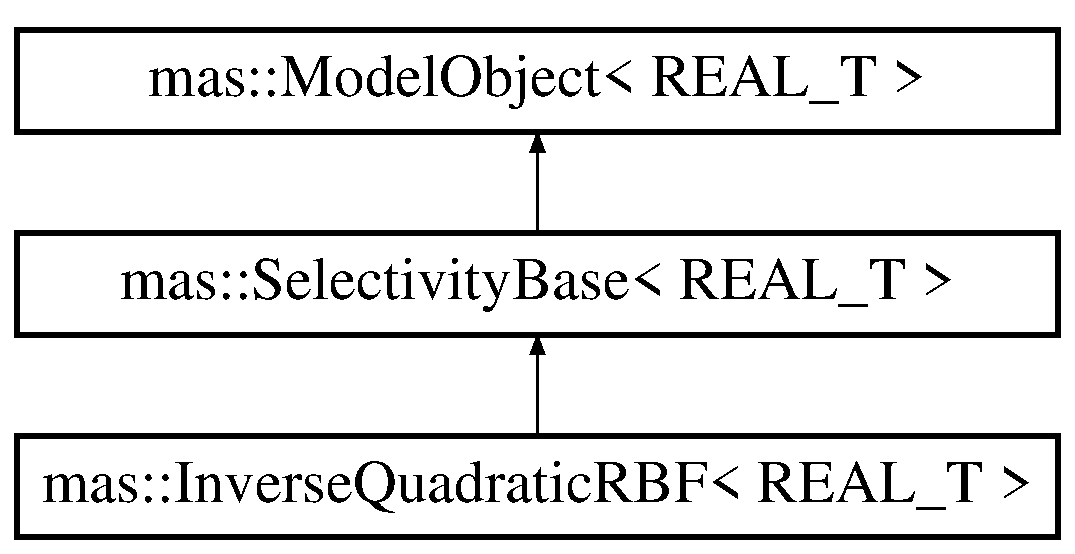
\includegraphics[height=3.000000cm]{structmas_1_1_inverse_quadratic_r_b_f}
\end{center}
\end{figure}
\subsection*{Public Types}
\begin{DoxyCompactItemize}
\item 
typedef \hyperlink{structmas_1_1_variable_trait}{Variable\-Trait}$<$ R\-E\-A\-L\-\_\-\-T $>$\\*
\-::\hyperlink{structmas_1_1_inverse_quadratic_r_b_f_aa73b147b14646342ba3141b53752cb1b}{variable} \hyperlink{structmas_1_1_inverse_quadratic_r_b_f_aa73b147b14646342ba3141b53752cb1b}{variable}
\end{DoxyCompactItemize}
\subsection*{Public Member Functions}
\begin{DoxyCompactItemize}
\item 
const \hyperlink{structmas_1_1_inverse_quadratic_r_b_f_aa73b147b14646342ba3141b53752cb1b}{variable} \hyperlink{structmas_1_1_inverse_quadratic_r_b_f_a56cc3b331603a6e1df6b861d827bed79}{Distance} (const \hyperlink{structmas_1_1_inverse_quadratic_r_b_f_aa73b147b14646342ba3141b53752cb1b}{variable} \&a)
\item 
virtual const \hyperlink{structmas_1_1_inverse_quadratic_r_b_f_aa73b147b14646342ba3141b53752cb1b}{variable} \hyperlink{structmas_1_1_inverse_quadratic_r_b_f_a4753edb34b33f783ae2c645cc16a607c}{Evaluate} (const \hyperlink{structmas_1_1_inverse_quadratic_r_b_f_aa73b147b14646342ba3141b53752cb1b}{variable} \&a)
\item 
virtual const \hyperlink{structmas_1_1_inverse_quadratic_r_b_f_aa73b147b14646342ba3141b53752cb1b}{variable} \hyperlink{structmas_1_1_inverse_quadratic_r_b_f_a326a1c19949fa3b309fbfc38a4c85dc7}{Evaluate} (const std\-::vector$<$ \hyperlink{structmas_1_1_inverse_quadratic_r_b_f_aa73b147b14646342ba3141b53752cb1b}{variable} $>$ \&ages, size\-\_\-t index)
\item 
virtual const std\-::string \hyperlink{structmas_1_1_inverse_quadratic_r_b_f_a59195ed8bba6ab30d34fa1d204c264bf}{To\-J\-S\-O\-N\-String} ()
\item 
virtual const std\-::string \hyperlink{structmas_1_1_inverse_quadratic_r_b_f_a2733866b50a4a7ae667f50334fdccc27}{Name} ()
\item 
virtual std\-::string \hyperlink{structmas_1_1_inverse_quadratic_r_b_f_a51999c40500b4bedc5bb24a1b0b87bb7}{To\-String} ()
\end{DoxyCompactItemize}
\subsection*{Public Attributes}
\begin{DoxyCompactItemize}
\item 
\hyperlink{structmas_1_1_inverse_quadratic_r_b_f_aa73b147b14646342ba3141b53752cb1b}{variable} \hyperlink{structmas_1_1_inverse_quadratic_r_b_f_a38cd5584cc6b9204720c0d8263095984}{centroid} = 1.\-1
\item 
\hyperlink{structmas_1_1_inverse_quadratic_r_b_f_aa73b147b14646342ba3141b53752cb1b}{variable} \hyperlink{structmas_1_1_inverse_quadratic_r_b_f_af694b194e549a0883ba192dec7bd9923}{epsilon} = 1.\-0
\item 
std\-::vector$<$ \hyperlink{structmas_1_1_inverse_quadratic_r_b_f_aa73b147b14646342ba3141b53752cb1b}{variable} $>$ \hyperlink{structmas_1_1_inverse_quadratic_r_b_f_a1e927c1c6b714eb3ca9e6deece81e60e}{w}
\end{DoxyCompactItemize}


\subsection{Detailed Description}
\subsubsection*{template$<$typename R\-E\-A\-L\-\_\-\-T$>$struct mas\-::\-Inverse\-Quadratic\-R\-B\-F$<$ R\-E\-A\-L\-\_\-\-T $>$}



Definition at line 243 of file Selectivity.\-hpp.



\subsection{Member Typedef Documentation}
\hypertarget{structmas_1_1_inverse_quadratic_r_b_f_aa73b147b14646342ba3141b53752cb1b}{\index{mas\-::\-Inverse\-Quadratic\-R\-B\-F@{mas\-::\-Inverse\-Quadratic\-R\-B\-F}!variable@{variable}}
\index{variable@{variable}!mas::InverseQuadraticRBF@{mas\-::\-Inverse\-Quadratic\-R\-B\-F}}
\subsubsection[{variable}]{\setlength{\rightskip}{0pt plus 5cm}template$<$typename R\-E\-A\-L\-\_\-\-T $>$ typedef {\bf Variable\-Trait}$<$R\-E\-A\-L\-\_\-\-T$>$\-::{\bf variable} {\bf mas\-::\-Inverse\-Quadratic\-R\-B\-F}$<$ R\-E\-A\-L\-\_\-\-T $>$\-::{\bf variable}}}\label{structmas_1_1_inverse_quadratic_r_b_f_aa73b147b14646342ba3141b53752cb1b}


Definition at line 244 of file Selectivity.\-hpp.



\subsection{Member Function Documentation}
\hypertarget{structmas_1_1_inverse_quadratic_r_b_f_a56cc3b331603a6e1df6b861d827bed79}{\index{mas\-::\-Inverse\-Quadratic\-R\-B\-F@{mas\-::\-Inverse\-Quadratic\-R\-B\-F}!Distance@{Distance}}
\index{Distance@{Distance}!mas::InverseQuadraticRBF@{mas\-::\-Inverse\-Quadratic\-R\-B\-F}}
\subsubsection[{Distance}]{\setlength{\rightskip}{0pt plus 5cm}template$<$typename R\-E\-A\-L\-\_\-\-T $>$ const {\bf variable} {\bf mas\-::\-Inverse\-Quadratic\-R\-B\-F}$<$ R\-E\-A\-L\-\_\-\-T $>$\-::Distance (
\begin{DoxyParamCaption}
\item[{const {\bf variable} \&}]{a}
\end{DoxyParamCaption}
)\hspace{0.3cm}{\ttfamily [inline]}}}\label{structmas_1_1_inverse_quadratic_r_b_f_a56cc3b331603a6e1df6b861d827bed79}


Definition at line 249 of file Selectivity.\-hpp.

\hypertarget{structmas_1_1_inverse_quadratic_r_b_f_a4753edb34b33f783ae2c645cc16a607c}{\index{mas\-::\-Inverse\-Quadratic\-R\-B\-F@{mas\-::\-Inverse\-Quadratic\-R\-B\-F}!Evaluate@{Evaluate}}
\index{Evaluate@{Evaluate}!mas::InverseQuadraticRBF@{mas\-::\-Inverse\-Quadratic\-R\-B\-F}}
\subsubsection[{Evaluate}]{\setlength{\rightskip}{0pt plus 5cm}template$<$typename R\-E\-A\-L\-\_\-\-T $>$ virtual const {\bf variable} {\bf mas\-::\-Inverse\-Quadratic\-R\-B\-F}$<$ R\-E\-A\-L\-\_\-\-T $>$\-::Evaluate (
\begin{DoxyParamCaption}
\item[{const {\bf variable} \&}]{a}
\end{DoxyParamCaption}
)\hspace{0.3cm}{\ttfamily [inline]}, {\ttfamily [virtual]}}}\label{structmas_1_1_inverse_quadratic_r_b_f_a4753edb34b33f783ae2c645cc16a607c}
Age based inverse quadratic rbf selectivity 
\begin{DoxyParams}{Parameters}
{\em a} & -\/ age \\
\hline
\end{DoxyParams}
\begin{DoxyReturn}{Returns}

\end{DoxyReturn}


Implements \hyperlink{structmas_1_1_selectivity_base_a1c26fb2107d380ac4540271280031bf4}{mas\-::\-Selectivity\-Base$<$ R\-E\-A\-L\-\_\-\-T $>$}.



Definition at line 258 of file Selectivity.\-hpp.

\hypertarget{structmas_1_1_inverse_quadratic_r_b_f_a326a1c19949fa3b309fbfc38a4c85dc7}{\index{mas\-::\-Inverse\-Quadratic\-R\-B\-F@{mas\-::\-Inverse\-Quadratic\-R\-B\-F}!Evaluate@{Evaluate}}
\index{Evaluate@{Evaluate}!mas::InverseQuadraticRBF@{mas\-::\-Inverse\-Quadratic\-R\-B\-F}}
\subsubsection[{Evaluate}]{\setlength{\rightskip}{0pt plus 5cm}template$<$typename R\-E\-A\-L\-\_\-\-T $>$ virtual const {\bf variable} {\bf mas\-::\-Inverse\-Quadratic\-R\-B\-F}$<$ R\-E\-A\-L\-\_\-\-T $>$\-::Evaluate (
\begin{DoxyParamCaption}
\item[{const std\-::vector$<$ {\bf variable} $>$ \&}]{ages, }
\item[{size\-\_\-t}]{index}
\end{DoxyParamCaption}
)\hspace{0.3cm}{\ttfamily [inline]}, {\ttfamily [virtual]}}}\label{structmas_1_1_inverse_quadratic_r_b_f_a326a1c19949fa3b309fbfc38a4c85dc7}


Implements \hyperlink{structmas_1_1_selectivity_base_a52058fc9fe373bcc6deebd43bfc3f402}{mas\-::\-Selectivity\-Base$<$ R\-E\-A\-L\-\_\-\-T $>$}.



Definition at line 262 of file Selectivity.\-hpp.

\hypertarget{structmas_1_1_inverse_quadratic_r_b_f_a2733866b50a4a7ae667f50334fdccc27}{\index{mas\-::\-Inverse\-Quadratic\-R\-B\-F@{mas\-::\-Inverse\-Quadratic\-R\-B\-F}!Name@{Name}}
\index{Name@{Name}!mas::InverseQuadraticRBF@{mas\-::\-Inverse\-Quadratic\-R\-B\-F}}
\subsubsection[{Name}]{\setlength{\rightskip}{0pt plus 5cm}template$<$typename R\-E\-A\-L\-\_\-\-T $>$ virtual const std\-::string {\bf mas\-::\-Inverse\-Quadratic\-R\-B\-F}$<$ R\-E\-A\-L\-\_\-\-T $>$\-::Name (
\begin{DoxyParamCaption}
{}
\end{DoxyParamCaption}
)\hspace{0.3cm}{\ttfamily [inline]}, {\ttfamily [virtual]}}}\label{structmas_1_1_inverse_quadratic_r_b_f_a2733866b50a4a7ae667f50334fdccc27}


Reimplemented from \hyperlink{structmas_1_1_selectivity_base_ad14deefa4cddcc1c93ef17cc0a3e566a}{mas\-::\-Selectivity\-Base$<$ R\-E\-A\-L\-\_\-\-T $>$}.



Definition at line 285 of file Selectivity.\-hpp.

\hypertarget{structmas_1_1_inverse_quadratic_r_b_f_a59195ed8bba6ab30d34fa1d204c264bf}{\index{mas\-::\-Inverse\-Quadratic\-R\-B\-F@{mas\-::\-Inverse\-Quadratic\-R\-B\-F}!To\-J\-S\-O\-N\-String@{To\-J\-S\-O\-N\-String}}
\index{To\-J\-S\-O\-N\-String@{To\-J\-S\-O\-N\-String}!mas::InverseQuadraticRBF@{mas\-::\-Inverse\-Quadratic\-R\-B\-F}}
\subsubsection[{To\-J\-S\-O\-N\-String}]{\setlength{\rightskip}{0pt plus 5cm}template$<$typename R\-E\-A\-L\-\_\-\-T $>$ virtual const std\-::string {\bf mas\-::\-Inverse\-Quadratic\-R\-B\-F}$<$ R\-E\-A\-L\-\_\-\-T $>$\-::To\-J\-S\-O\-N\-String (
\begin{DoxyParamCaption}
{}
\end{DoxyParamCaption}
)\hspace{0.3cm}{\ttfamily [inline]}, {\ttfamily [virtual]}}}\label{structmas_1_1_inverse_quadratic_r_b_f_a59195ed8bba6ab30d34fa1d204c264bf}


Reimplemented from \hyperlink{structmas_1_1_model_object_af40b3c89b11919fc5aea21dcf1cd027b}{mas\-::\-Model\-Object$<$ R\-E\-A\-L\-\_\-\-T $>$}.



Definition at line 273 of file Selectivity.\-hpp.

\hypertarget{structmas_1_1_inverse_quadratic_r_b_f_a51999c40500b4bedc5bb24a1b0b87bb7}{\index{mas\-::\-Inverse\-Quadratic\-R\-B\-F@{mas\-::\-Inverse\-Quadratic\-R\-B\-F}!To\-String@{To\-String}}
\index{To\-String@{To\-String}!mas::InverseQuadraticRBF@{mas\-::\-Inverse\-Quadratic\-R\-B\-F}}
\subsubsection[{To\-String}]{\setlength{\rightskip}{0pt plus 5cm}template$<$typename R\-E\-A\-L\-\_\-\-T $>$ virtual std\-::string {\bf mas\-::\-Inverse\-Quadratic\-R\-B\-F}$<$ R\-E\-A\-L\-\_\-\-T $>$\-::To\-String (
\begin{DoxyParamCaption}
{}
\end{DoxyParamCaption}
)\hspace{0.3cm}{\ttfamily [inline]}, {\ttfamily [virtual]}}}\label{structmas_1_1_inverse_quadratic_r_b_f_a51999c40500b4bedc5bb24a1b0b87bb7}


Reimplemented from \hyperlink{structmas_1_1_model_object_a8eaf6c7c52e42ea8869aefa318358cb5}{mas\-::\-Model\-Object$<$ R\-E\-A\-L\-\_\-\-T $>$}.



Definition at line 289 of file Selectivity.\-hpp.



\subsection{Member Data Documentation}
\hypertarget{structmas_1_1_inverse_quadratic_r_b_f_a38cd5584cc6b9204720c0d8263095984}{\index{mas\-::\-Inverse\-Quadratic\-R\-B\-F@{mas\-::\-Inverse\-Quadratic\-R\-B\-F}!centroid@{centroid}}
\index{centroid@{centroid}!mas::InverseQuadraticRBF@{mas\-::\-Inverse\-Quadratic\-R\-B\-F}}
\subsubsection[{centroid}]{\setlength{\rightskip}{0pt plus 5cm}template$<$typename R\-E\-A\-L\-\_\-\-T $>$ {\bf variable} {\bf mas\-::\-Inverse\-Quadratic\-R\-B\-F}$<$ R\-E\-A\-L\-\_\-\-T $>$\-::centroid = 1.\-1}}\label{structmas_1_1_inverse_quadratic_r_b_f_a38cd5584cc6b9204720c0d8263095984}


Definition at line 245 of file Selectivity.\-hpp.

\hypertarget{structmas_1_1_inverse_quadratic_r_b_f_af694b194e549a0883ba192dec7bd9923}{\index{mas\-::\-Inverse\-Quadratic\-R\-B\-F@{mas\-::\-Inverse\-Quadratic\-R\-B\-F}!epsilon@{epsilon}}
\index{epsilon@{epsilon}!mas::InverseQuadraticRBF@{mas\-::\-Inverse\-Quadratic\-R\-B\-F}}
\subsubsection[{epsilon}]{\setlength{\rightskip}{0pt plus 5cm}template$<$typename R\-E\-A\-L\-\_\-\-T $>$ {\bf variable} {\bf mas\-::\-Inverse\-Quadratic\-R\-B\-F}$<$ R\-E\-A\-L\-\_\-\-T $>$\-::epsilon = 1.\-0}}\label{structmas_1_1_inverse_quadratic_r_b_f_af694b194e549a0883ba192dec7bd9923}


Definition at line 246 of file Selectivity.\-hpp.

\hypertarget{structmas_1_1_inverse_quadratic_r_b_f_a1e927c1c6b714eb3ca9e6deece81e60e}{\index{mas\-::\-Inverse\-Quadratic\-R\-B\-F@{mas\-::\-Inverse\-Quadratic\-R\-B\-F}!w@{w}}
\index{w@{w}!mas::InverseQuadraticRBF@{mas\-::\-Inverse\-Quadratic\-R\-B\-F}}
\subsubsection[{w}]{\setlength{\rightskip}{0pt plus 5cm}template$<$typename R\-E\-A\-L\-\_\-\-T $>$ std\-::vector$<${\bf variable}$>$ {\bf mas\-::\-Inverse\-Quadratic\-R\-B\-F}$<$ R\-E\-A\-L\-\_\-\-T $>$\-::w}}\label{structmas_1_1_inverse_quadratic_r_b_f_a1e927c1c6b714eb3ca9e6deece81e60e}


Definition at line 247 of file Selectivity.\-hpp.



The documentation for this struct was generated from the following file\-:\begin{DoxyCompactItemize}
\item 
/home/oppy/\-Net\-Beans\-Projects/mas/\hyperlink{_selectivity_8hpp}{Selectivity.\-hpp}\end{DoxyCompactItemize}

\hypertarget{structmas_1_1_logistic_fec}{\section{mas\-:\-:Logistic\-Fec$<$ R\-E\-A\-L\-\_\-\-T $>$ Struct Template Reference}
\label{structmas_1_1_logistic_fec}\index{mas\-::\-Logistic\-Fec$<$ R\-E\-A\-L\-\_\-\-T $>$@{mas\-::\-Logistic\-Fec$<$ R\-E\-A\-L\-\_\-\-T $>$}}
}


{\ttfamily \#include $<$Fecundity.\-hpp$>$}

Inheritance diagram for mas\-:\-:Logistic\-Fec$<$ R\-E\-A\-L\-\_\-\-T $>$\-:\begin{figure}[H]
\begin{center}
\leavevmode
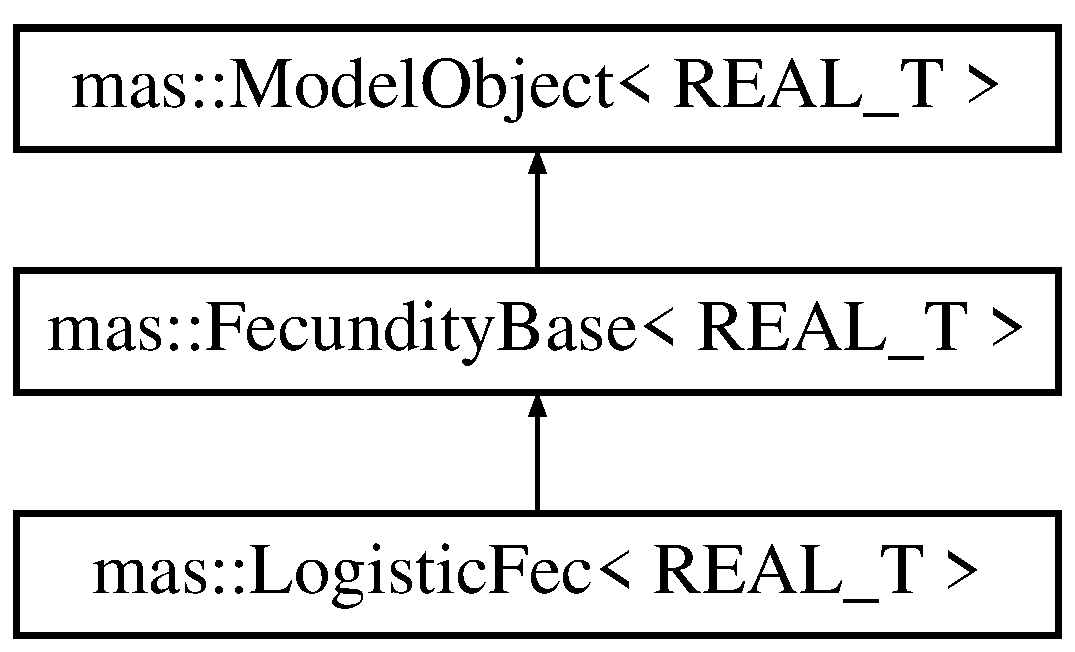
\includegraphics[height=3.000000cm]{structmas_1_1_logistic_fec}
\end{center}
\end{figure}
\subsection*{Public Types}
\begin{DoxyCompactItemize}
\item 
typedef \hyperlink{structmas_1_1_variable_trait}{Variable\-Trait}$<$ R\-E\-A\-L\-\_\-\-T $>$\\*
\-::\hyperlink{structmas_1_1_logistic_fec_ad7f5125508249b28ef04b00d022d8055}{variable} \hyperlink{structmas_1_1_logistic_fec_ad7f5125508249b28ef04b00d022d8055}{variable}
\end{DoxyCompactItemize}
\subsection*{Public Member Functions}
\begin{DoxyCompactItemize}
\item 
virtual const \hyperlink{structmas_1_1_logistic_fec_ad7f5125508249b28ef04b00d022d8055}{variable} \hyperlink{structmas_1_1_logistic_fec_a39ba0a3a580b10ec1cf5ad2e3d24a029}{Evaluate} (const int \&sex, const \hyperlink{structmas_1_1_logistic_fec_ad7f5125508249b28ef04b00d022d8055}{variable} \&age)
\item 
virtual const std\-::string \hyperlink{structmas_1_1_logistic_fec_a2c6a92c26528208819f69dabc1859956}{Name} ()
\end{DoxyCompactItemize}
\subsection*{Public Attributes}
\begin{DoxyCompactItemize}
\item 
\hyperlink{structmas_1_1_logistic_fec_ad7f5125508249b28ef04b00d022d8055}{variable} \hyperlink{structmas_1_1_logistic_fec_a6e72c6de9d6e0a69fea2c9fe580bedb3}{a50}
\item 
\hyperlink{structmas_1_1_logistic_fec_ad7f5125508249b28ef04b00d022d8055}{variable} \hyperlink{structmas_1_1_logistic_fec_a69f62cb6f7c2e37af6c8cebc041e864e}{s}
\end{DoxyCompactItemize}


\subsection{Detailed Description}
\subsubsection*{template$<$typename R\-E\-A\-L\-\_\-\-T$>$struct mas\-::\-Logistic\-Fec$<$ R\-E\-A\-L\-\_\-\-T $>$}



Definition at line 55 of file Fecundity.\-hpp.



\subsection{Member Typedef Documentation}
\hypertarget{structmas_1_1_logistic_fec_ad7f5125508249b28ef04b00d022d8055}{\index{mas\-::\-Logistic\-Fec@{mas\-::\-Logistic\-Fec}!variable@{variable}}
\index{variable@{variable}!mas::LogisticFec@{mas\-::\-Logistic\-Fec}}
\subsubsection[{variable}]{\setlength{\rightskip}{0pt plus 5cm}template$<$typename R\-E\-A\-L\-\_\-\-T $>$ typedef {\bf Variable\-Trait}$<$R\-E\-A\-L\-\_\-\-T$>$\-::{\bf variable} {\bf mas\-::\-Logistic\-Fec}$<$ R\-E\-A\-L\-\_\-\-T $>$\-::{\bf variable}}}\label{structmas_1_1_logistic_fec_ad7f5125508249b28ef04b00d022d8055}


Definition at line 56 of file Fecundity.\-hpp.



\subsection{Member Function Documentation}
\hypertarget{structmas_1_1_logistic_fec_a39ba0a3a580b10ec1cf5ad2e3d24a029}{\index{mas\-::\-Logistic\-Fec@{mas\-::\-Logistic\-Fec}!Evaluate@{Evaluate}}
\index{Evaluate@{Evaluate}!mas::LogisticFec@{mas\-::\-Logistic\-Fec}}
\subsubsection[{Evaluate}]{\setlength{\rightskip}{0pt plus 5cm}template$<$typename R\-E\-A\-L\-\_\-\-T $>$ virtual const {\bf variable} {\bf mas\-::\-Logistic\-Fec}$<$ R\-E\-A\-L\-\_\-\-T $>$\-::Evaluate (
\begin{DoxyParamCaption}
\item[{const int \&}]{sex, }
\item[{const {\bf variable} \&}]{age}
\end{DoxyParamCaption}
)\hspace{0.3cm}{\ttfamily [inline]}, {\ttfamily [virtual]}}}\label{structmas_1_1_logistic_fec_a39ba0a3a580b10ec1cf5ad2e3d24a029}
Age based logistic maturity


\begin{DoxyParams}{Parameters}
{\em sex} & \\
\hline
{\em age} & \\
\hline
\end{DoxyParams}
\begin{DoxyReturn}{Returns}
fraction\-\_\-mature 
\end{DoxyReturn}


Implements \hyperlink{structmas_1_1_fecundity_base_a44573d4082a65920010d9d20ed2d8e14}{mas\-::\-Fecundity\-Base$<$ R\-E\-A\-L\-\_\-\-T $>$}.



Definition at line 67 of file Fecundity.\-hpp.

\hypertarget{structmas_1_1_logistic_fec_a2c6a92c26528208819f69dabc1859956}{\index{mas\-::\-Logistic\-Fec@{mas\-::\-Logistic\-Fec}!Name@{Name}}
\index{Name@{Name}!mas::LogisticFec@{mas\-::\-Logistic\-Fec}}
\subsubsection[{Name}]{\setlength{\rightskip}{0pt plus 5cm}template$<$typename R\-E\-A\-L\-\_\-\-T $>$ virtual const std\-::string {\bf mas\-::\-Logistic\-Fec}$<$ R\-E\-A\-L\-\_\-\-T $>$\-::Name (
\begin{DoxyParamCaption}
{}
\end{DoxyParamCaption}
)\hspace{0.3cm}{\ttfamily [inline]}, {\ttfamily [virtual]}}}\label{structmas_1_1_logistic_fec_a2c6a92c26528208819f69dabc1859956}


Reimplemented from \hyperlink{structmas_1_1_fecundity_base_a5a0ca3b02791910dd012a30f1c2bf2a8}{mas\-::\-Fecundity\-Base$<$ R\-E\-A\-L\-\_\-\-T $>$}.



Definition at line 71 of file Fecundity.\-hpp.



\subsection{Member Data Documentation}
\hypertarget{structmas_1_1_logistic_fec_a6e72c6de9d6e0a69fea2c9fe580bedb3}{\index{mas\-::\-Logistic\-Fec@{mas\-::\-Logistic\-Fec}!a50@{a50}}
\index{a50@{a50}!mas::LogisticFec@{mas\-::\-Logistic\-Fec}}
\subsubsection[{a50}]{\setlength{\rightskip}{0pt plus 5cm}template$<$typename R\-E\-A\-L\-\_\-\-T $>$ {\bf variable} {\bf mas\-::\-Logistic\-Fec}$<$ R\-E\-A\-L\-\_\-\-T $>$\-::a50}}\label{structmas_1_1_logistic_fec_a6e72c6de9d6e0a69fea2c9fe580bedb3}


Definition at line 57 of file Fecundity.\-hpp.

\hypertarget{structmas_1_1_logistic_fec_a69f62cb6f7c2e37af6c8cebc041e864e}{\index{mas\-::\-Logistic\-Fec@{mas\-::\-Logistic\-Fec}!s@{s}}
\index{s@{s}!mas::LogisticFec@{mas\-::\-Logistic\-Fec}}
\subsubsection[{s}]{\setlength{\rightskip}{0pt plus 5cm}template$<$typename R\-E\-A\-L\-\_\-\-T $>$ {\bf variable} {\bf mas\-::\-Logistic\-Fec}$<$ R\-E\-A\-L\-\_\-\-T $>$\-::s}}\label{structmas_1_1_logistic_fec_a69f62cb6f7c2e37af6c8cebc041e864e}


Definition at line 58 of file Fecundity.\-hpp.



The documentation for this struct was generated from the following file\-:\begin{DoxyCompactItemize}
\item 
/home/oppy/\-Net\-Beans\-Projects/mas/\hyperlink{_fecundity_8hpp}{Fecundity.\-hpp}\end{DoxyCompactItemize}

\hypertarget{structmas_1_1_logistic_sel}{\section{mas\-:\-:Logistic\-Sel$<$ R\-E\-A\-L\-\_\-\-T $>$ Struct Template Reference}
\label{structmas_1_1_logistic_sel}\index{mas\-::\-Logistic\-Sel$<$ R\-E\-A\-L\-\_\-\-T $>$@{mas\-::\-Logistic\-Sel$<$ R\-E\-A\-L\-\_\-\-T $>$}}
}


{\ttfamily \#include $<$Selectivity.\-hpp$>$}

Inheritance diagram for mas\-:\-:Logistic\-Sel$<$ R\-E\-A\-L\-\_\-\-T $>$\-:\begin{figure}[H]
\begin{center}
\leavevmode
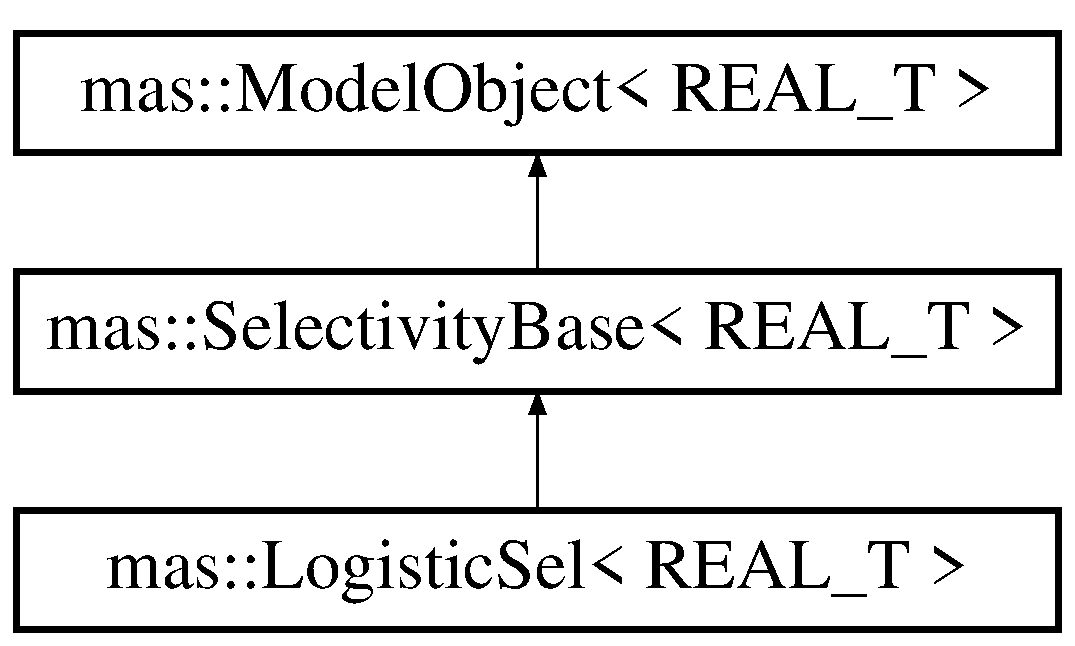
\includegraphics[height=3.000000cm]{structmas_1_1_logistic_sel}
\end{center}
\end{figure}
\subsection*{Public Types}
\begin{DoxyCompactItemize}
\item 
typedef \hyperlink{structmas_1_1_variable_trait}{Variable\-Trait}$<$ R\-E\-A\-L\-\_\-\-T $>$\\*
\-::\hyperlink{structmas_1_1_logistic_sel_afd5ce39e0aaab3c2bbe4cdab00f0273e}{variable} \hyperlink{structmas_1_1_logistic_sel_afd5ce39e0aaab3c2bbe4cdab00f0273e}{variable}
\end{DoxyCompactItemize}
\subsection*{Public Member Functions}
\begin{DoxyCompactItemize}
\item 
virtual const \hyperlink{structmas_1_1_logistic_sel_afd5ce39e0aaab3c2bbe4cdab00f0273e}{variable} \hyperlink{structmas_1_1_logistic_sel_a2e7590748bd817f5a019c633213488cc}{Evaluate} (const \hyperlink{structmas_1_1_logistic_sel_afd5ce39e0aaab3c2bbe4cdab00f0273e}{variable} \&a)
\item 
virtual const \hyperlink{structmas_1_1_logistic_sel_afd5ce39e0aaab3c2bbe4cdab00f0273e}{variable} \hyperlink{structmas_1_1_logistic_sel_ae646dfffa37e9202381fb0c1879016ee}{Evaluate} (const std\-::vector$<$ \hyperlink{structmas_1_1_logistic_sel_afd5ce39e0aaab3c2bbe4cdab00f0273e}{variable} $>$ \&ages, size\-\_\-t index)
\item 
virtual const std\-::string \hyperlink{structmas_1_1_logistic_sel_afa9abd8671cf8d82a6973c4369741b41}{To\-J\-S\-O\-N\-String} ()
\item 
virtual const std\-::string \hyperlink{structmas_1_1_logistic_sel_a58f669fc791e7e86ef70820dbbed35ba}{Name} ()
\item 
virtual std\-::string \hyperlink{structmas_1_1_logistic_sel_a625cc43faa89094c25da029a827ba638}{To\-String} ()
\end{DoxyCompactItemize}
\subsection*{Public Attributes}
\begin{DoxyCompactItemize}
\item 
\hyperlink{structmas_1_1_logistic_sel_afd5ce39e0aaab3c2bbe4cdab00f0273e}{variable} \hyperlink{structmas_1_1_logistic_sel_a2aab2cd35ed2fa7fb0780c810fefb91a}{a50}
\item 
\hyperlink{structmas_1_1_logistic_sel_afd5ce39e0aaab3c2bbe4cdab00f0273e}{variable} \hyperlink{structmas_1_1_logistic_sel_a2358849095acf217deae4f595b670d2f}{s}
\end{DoxyCompactItemize}


\subsection{Detailed Description}
\subsubsection*{template$<$typename R\-E\-A\-L\-\_\-\-T$>$struct mas\-::\-Logistic\-Sel$<$ R\-E\-A\-L\-\_\-\-T $>$}



Definition at line 57 of file Selectivity.\-hpp.



\subsection{Member Typedef Documentation}
\hypertarget{structmas_1_1_logistic_sel_afd5ce39e0aaab3c2bbe4cdab00f0273e}{\index{mas\-::\-Logistic\-Sel@{mas\-::\-Logistic\-Sel}!variable@{variable}}
\index{variable@{variable}!mas::LogisticSel@{mas\-::\-Logistic\-Sel}}
\subsubsection[{variable}]{\setlength{\rightskip}{0pt plus 5cm}template$<$typename R\-E\-A\-L\-\_\-\-T $>$ typedef {\bf Variable\-Trait}$<$R\-E\-A\-L\-\_\-\-T$>$\-::{\bf variable} {\bf mas\-::\-Logistic\-Sel}$<$ R\-E\-A\-L\-\_\-\-T $>$\-::{\bf variable}}}\label{structmas_1_1_logistic_sel_afd5ce39e0aaab3c2bbe4cdab00f0273e}


Definition at line 58 of file Selectivity.\-hpp.



\subsection{Member Function Documentation}
\hypertarget{structmas_1_1_logistic_sel_a2e7590748bd817f5a019c633213488cc}{\index{mas\-::\-Logistic\-Sel@{mas\-::\-Logistic\-Sel}!Evaluate@{Evaluate}}
\index{Evaluate@{Evaluate}!mas::LogisticSel@{mas\-::\-Logistic\-Sel}}
\subsubsection[{Evaluate}]{\setlength{\rightskip}{0pt plus 5cm}template$<$typename R\-E\-A\-L\-\_\-\-T $>$ virtual const {\bf variable} {\bf mas\-::\-Logistic\-Sel}$<$ R\-E\-A\-L\-\_\-\-T $>$\-::Evaluate (
\begin{DoxyParamCaption}
\item[{const {\bf variable} \&}]{a}
\end{DoxyParamCaption}
)\hspace{0.3cm}{\ttfamily [inline]}, {\ttfamily [virtual]}}}\label{structmas_1_1_logistic_sel_a2e7590748bd817f5a019c633213488cc}
Age based logistic selectivity 
\begin{DoxyParams}{Parameters}
{\em a} & -\/ age \\
\hline
\end{DoxyParams}
\begin{DoxyReturn}{Returns}

\end{DoxyReturn}


Implements \hyperlink{structmas_1_1_selectivity_base_a1c26fb2107d380ac4540271280031bf4}{mas\-::\-Selectivity\-Base$<$ R\-E\-A\-L\-\_\-\-T $>$}.



Definition at line 67 of file Selectivity.\-hpp.

\hypertarget{structmas_1_1_logistic_sel_ae646dfffa37e9202381fb0c1879016ee}{\index{mas\-::\-Logistic\-Sel@{mas\-::\-Logistic\-Sel}!Evaluate@{Evaluate}}
\index{Evaluate@{Evaluate}!mas::LogisticSel@{mas\-::\-Logistic\-Sel}}
\subsubsection[{Evaluate}]{\setlength{\rightskip}{0pt plus 5cm}template$<$typename R\-E\-A\-L\-\_\-\-T $>$ virtual const {\bf variable} {\bf mas\-::\-Logistic\-Sel}$<$ R\-E\-A\-L\-\_\-\-T $>$\-::Evaluate (
\begin{DoxyParamCaption}
\item[{const std\-::vector$<$ {\bf variable} $>$ \&}]{ages, }
\item[{size\-\_\-t}]{index}
\end{DoxyParamCaption}
)\hspace{0.3cm}{\ttfamily [inline]}, {\ttfamily [virtual]}}}\label{structmas_1_1_logistic_sel_ae646dfffa37e9202381fb0c1879016ee}


Implements \hyperlink{structmas_1_1_selectivity_base_a52058fc9fe373bcc6deebd43bfc3f402}{mas\-::\-Selectivity\-Base$<$ R\-E\-A\-L\-\_\-\-T $>$}.



Definition at line 71 of file Selectivity.\-hpp.

\hypertarget{structmas_1_1_logistic_sel_a58f669fc791e7e86ef70820dbbed35ba}{\index{mas\-::\-Logistic\-Sel@{mas\-::\-Logistic\-Sel}!Name@{Name}}
\index{Name@{Name}!mas::LogisticSel@{mas\-::\-Logistic\-Sel}}
\subsubsection[{Name}]{\setlength{\rightskip}{0pt plus 5cm}template$<$typename R\-E\-A\-L\-\_\-\-T $>$ virtual const std\-::string {\bf mas\-::\-Logistic\-Sel}$<$ R\-E\-A\-L\-\_\-\-T $>$\-::Name (
\begin{DoxyParamCaption}
{}
\end{DoxyParamCaption}
)\hspace{0.3cm}{\ttfamily [inline]}, {\ttfamily [virtual]}}}\label{structmas_1_1_logistic_sel_a58f669fc791e7e86ef70820dbbed35ba}


Reimplemented from \hyperlink{structmas_1_1_selectivity_base_ad14deefa4cddcc1c93ef17cc0a3e566a}{mas\-::\-Selectivity\-Base$<$ R\-E\-A\-L\-\_\-\-T $>$}.



Definition at line 88 of file Selectivity.\-hpp.

\hypertarget{structmas_1_1_logistic_sel_afa9abd8671cf8d82a6973c4369741b41}{\index{mas\-::\-Logistic\-Sel@{mas\-::\-Logistic\-Sel}!To\-J\-S\-O\-N\-String@{To\-J\-S\-O\-N\-String}}
\index{To\-J\-S\-O\-N\-String@{To\-J\-S\-O\-N\-String}!mas::LogisticSel@{mas\-::\-Logistic\-Sel}}
\subsubsection[{To\-J\-S\-O\-N\-String}]{\setlength{\rightskip}{0pt plus 5cm}template$<$typename R\-E\-A\-L\-\_\-\-T $>$ virtual const std\-::string {\bf mas\-::\-Logistic\-Sel}$<$ R\-E\-A\-L\-\_\-\-T $>$\-::To\-J\-S\-O\-N\-String (
\begin{DoxyParamCaption}
{}
\end{DoxyParamCaption}
)\hspace{0.3cm}{\ttfamily [inline]}, {\ttfamily [virtual]}}}\label{structmas_1_1_logistic_sel_afa9abd8671cf8d82a6973c4369741b41}


Reimplemented from \hyperlink{structmas_1_1_model_object_af40b3c89b11919fc5aea21dcf1cd027b}{mas\-::\-Model\-Object$<$ R\-E\-A\-L\-\_\-\-T $>$}.



Definition at line 75 of file Selectivity.\-hpp.

\hypertarget{structmas_1_1_logistic_sel_a625cc43faa89094c25da029a827ba638}{\index{mas\-::\-Logistic\-Sel@{mas\-::\-Logistic\-Sel}!To\-String@{To\-String}}
\index{To\-String@{To\-String}!mas::LogisticSel@{mas\-::\-Logistic\-Sel}}
\subsubsection[{To\-String}]{\setlength{\rightskip}{0pt plus 5cm}template$<$typename R\-E\-A\-L\-\_\-\-T $>$ virtual std\-::string {\bf mas\-::\-Logistic\-Sel}$<$ R\-E\-A\-L\-\_\-\-T $>$\-::To\-String (
\begin{DoxyParamCaption}
{}
\end{DoxyParamCaption}
)\hspace{0.3cm}{\ttfamily [inline]}, {\ttfamily [virtual]}}}\label{structmas_1_1_logistic_sel_a625cc43faa89094c25da029a827ba638}


Reimplemented from \hyperlink{structmas_1_1_model_object_a8eaf6c7c52e42ea8869aefa318358cb5}{mas\-::\-Model\-Object$<$ R\-E\-A\-L\-\_\-\-T $>$}.



Definition at line 92 of file Selectivity.\-hpp.



\subsection{Member Data Documentation}
\hypertarget{structmas_1_1_logistic_sel_a2aab2cd35ed2fa7fb0780c810fefb91a}{\index{mas\-::\-Logistic\-Sel@{mas\-::\-Logistic\-Sel}!a50@{a50}}
\index{a50@{a50}!mas::LogisticSel@{mas\-::\-Logistic\-Sel}}
\subsubsection[{a50}]{\setlength{\rightskip}{0pt plus 5cm}template$<$typename R\-E\-A\-L\-\_\-\-T $>$ {\bf variable} {\bf mas\-::\-Logistic\-Sel}$<$ R\-E\-A\-L\-\_\-\-T $>$\-::a50}}\label{structmas_1_1_logistic_sel_a2aab2cd35ed2fa7fb0780c810fefb91a}


Definition at line 59 of file Selectivity.\-hpp.

\hypertarget{structmas_1_1_logistic_sel_a2358849095acf217deae4f595b670d2f}{\index{mas\-::\-Logistic\-Sel@{mas\-::\-Logistic\-Sel}!s@{s}}
\index{s@{s}!mas::LogisticSel@{mas\-::\-Logistic\-Sel}}
\subsubsection[{s}]{\setlength{\rightskip}{0pt plus 5cm}template$<$typename R\-E\-A\-L\-\_\-\-T $>$ {\bf variable} {\bf mas\-::\-Logistic\-Sel}$<$ R\-E\-A\-L\-\_\-\-T $>$\-::s}}\label{structmas_1_1_logistic_sel_a2358849095acf217deae4f595b670d2f}


Definition at line 60 of file Selectivity.\-hpp.



The documentation for this struct was generated from the following file\-:\begin{DoxyCompactItemize}
\item 
/home/oppy/\-Net\-Beans\-Projects/mas/\hyperlink{_selectivity_8hpp}{Selectivity.\-hpp}\end{DoxyCompactItemize}

\hypertarget{classmas_1_1_m_a_s}{\section{mas\-:\-:M\-A\-S$<$ R\-E\-A\-L\-\_\-\-T $>$ Class Template Reference}
\label{classmas_1_1_m_a_s}\index{mas\-::\-M\-A\-S$<$ R\-E\-A\-L\-\_\-\-T $>$@{mas\-::\-M\-A\-S$<$ R\-E\-A\-L\-\_\-\-T $>$}}
}


{\ttfamily \#include $<$M\-A\-S.\-hpp$>$}

\subsection*{Public Member Functions}
\begin{DoxyCompactItemize}
\item 
\hyperlink{classmas_1_1_m_a_s_abf7813e6c16681e7a6c66afacb80cb4f}{M\-A\-S} ()
\item 
\hyperlink{classmas_1_1_m_a_s_ad509033342a4fb5c6916e0d9346c610d}{M\-A\-S} (const \hyperlink{classmas_1_1_m_a_s}{M\-A\-S}$<$ R\-E\-A\-L\-\_\-\-T $>$ \&orig)
\item 
virtual \hyperlink{classmas_1_1_m_a_s_a21f64cb0d2110f201986a7b209a91f40}{$\sim$\-M\-A\-S} ()
\item 
void \hyperlink{classmas_1_1_m_a_s_afe6ea578b33a24f7ae7252a9ed5a595b}{Initialize} (const std\-::string \&config\-\_\-file, const std\-::string \&data\-\_\-file)
\item 
void \hyperlink{classmas_1_1_m_a_s_ad94002bbb3563647a927f5feef150573}{Run} (variable \&f)
\item 
void \hyperlink{classmas_1_1_m_a_s_aac0b9279e39863bea02e9b0eb3c3aa67}{Forecast} ()
\item 
void \hyperlink{classmas_1_1_m_a_s_afd76753b0c33bc0f0dd800c72f23afd5}{Report} ()
\end{DoxyCompactItemize}
\subsection*{Public Attributes}
\begin{DoxyCompactItemize}
\item 
int $\ast$ \hyperlink{classmas_1_1_m_a_s_a26d078a9930af45b319da8e6fdc5ae7d}{phase}
\item 
\hyperlink{classmas_1_1_information}{mas\-::\-Information}$<$ R\-E\-A\-L\-\_\-\-T $>$ \hyperlink{classmas_1_1_m_a_s_adf64a1ceccb1e52a43bc9ebebd87fd45}{info}
\end{DoxyCompactItemize}


\subsection{Detailed Description}
\subsubsection*{template$<$typename R\-E\-A\-L\-\_\-\-T$>$class mas\-::\-M\-A\-S$<$ R\-E\-A\-L\-\_\-\-T $>$}



Definition at line 41 of file M\-A\-S.\-hpp.



\subsection{Constructor \& Destructor Documentation}
\hypertarget{classmas_1_1_m_a_s_abf7813e6c16681e7a6c66afacb80cb4f}{\index{mas\-::\-M\-A\-S@{mas\-::\-M\-A\-S}!M\-A\-S@{M\-A\-S}}
\index{M\-A\-S@{M\-A\-S}!mas::MAS@{mas\-::\-M\-A\-S}}
\subsubsection[{M\-A\-S}]{\setlength{\rightskip}{0pt plus 5cm}template$<$typename R\-E\-A\-L\-\_\-\-T$>$ {\bf mas\-::\-M\-A\-S}$<$ R\-E\-A\-L\-\_\-\-T $>$\-::{\bf M\-A\-S} (
\begin{DoxyParamCaption}
{}
\end{DoxyParamCaption}
)\hspace{0.3cm}{\ttfamily [inline]}}}\label{classmas_1_1_m_a_s_abf7813e6c16681e7a6c66afacb80cb4f}


Definition at line 71 of file M\-A\-S.\-hpp.

\hypertarget{classmas_1_1_m_a_s_ad509033342a4fb5c6916e0d9346c610d}{\index{mas\-::\-M\-A\-S@{mas\-::\-M\-A\-S}!M\-A\-S@{M\-A\-S}}
\index{M\-A\-S@{M\-A\-S}!mas::MAS@{mas\-::\-M\-A\-S}}
\subsubsection[{M\-A\-S}]{\setlength{\rightskip}{0pt plus 5cm}template$<$typename R\-E\-A\-L\-\_\-\-T$>$ {\bf mas\-::\-M\-A\-S}$<$ R\-E\-A\-L\-\_\-\-T $>$\-::{\bf M\-A\-S} (
\begin{DoxyParamCaption}
\item[{const {\bf M\-A\-S}$<$ R\-E\-A\-L\-\_\-\-T $>$ \&}]{orig}
\end{DoxyParamCaption}
)\hspace{0.3cm}{\ttfamily [inline]}}}\label{classmas_1_1_m_a_s_ad509033342a4fb5c6916e0d9346c610d}


Definition at line 74 of file M\-A\-S.\-hpp.

\hypertarget{classmas_1_1_m_a_s_a21f64cb0d2110f201986a7b209a91f40}{\index{mas\-::\-M\-A\-S@{mas\-::\-M\-A\-S}!$\sim$\-M\-A\-S@{$\sim$\-M\-A\-S}}
\index{$\sim$\-M\-A\-S@{$\sim$\-M\-A\-S}!mas::MAS@{mas\-::\-M\-A\-S}}
\subsubsection[{$\sim$\-M\-A\-S}]{\setlength{\rightskip}{0pt plus 5cm}template$<$typename R\-E\-A\-L\-\_\-\-T$>$ virtual {\bf mas\-::\-M\-A\-S}$<$ R\-E\-A\-L\-\_\-\-T $>$\-::$\sim${\bf M\-A\-S} (
\begin{DoxyParamCaption}
{}
\end{DoxyParamCaption}
)\hspace{0.3cm}{\ttfamily [inline]}, {\ttfamily [virtual]}}}\label{classmas_1_1_m_a_s_a21f64cb0d2110f201986a7b209a91f40}


Definition at line 77 of file M\-A\-S.\-hpp.



\subsection{Member Function Documentation}
\hypertarget{classmas_1_1_m_a_s_aac0b9279e39863bea02e9b0eb3c3aa67}{\index{mas\-::\-M\-A\-S@{mas\-::\-M\-A\-S}!Forecast@{Forecast}}
\index{Forecast@{Forecast}!mas::MAS@{mas\-::\-M\-A\-S}}
\subsubsection[{Forecast}]{\setlength{\rightskip}{0pt plus 5cm}template$<$typename R\-E\-A\-L\-\_\-\-T$>$ void {\bf mas\-::\-M\-A\-S}$<$ R\-E\-A\-L\-\_\-\-T $>$\-::Forecast (
\begin{DoxyParamCaption}
{}
\end{DoxyParamCaption}
)\hspace{0.3cm}{\ttfamily [inline]}}}\label{classmas_1_1_m_a_s_aac0b9279e39863bea02e9b0eb3c3aa67}


Definition at line 184 of file M\-A\-S.\-hpp.

\hypertarget{classmas_1_1_m_a_s_afe6ea578b33a24f7ae7252a9ed5a595b}{\index{mas\-::\-M\-A\-S@{mas\-::\-M\-A\-S}!Initialize@{Initialize}}
\index{Initialize@{Initialize}!mas::MAS@{mas\-::\-M\-A\-S}}
\subsubsection[{Initialize}]{\setlength{\rightskip}{0pt plus 5cm}template$<$typename R\-E\-A\-L\-\_\-\-T$>$ void {\bf mas\-::\-M\-A\-S}$<$ R\-E\-A\-L\-\_\-\-T $>$\-::Initialize (
\begin{DoxyParamCaption}
\item[{const std\-::string \&}]{config\-\_\-file, }
\item[{const std\-::string \&}]{data\-\_\-file}
\end{DoxyParamCaption}
)\hspace{0.3cm}{\ttfamily [inline]}}}\label{classmas_1_1_m_a_s_afe6ea578b33a24f7ae7252a9ed5a595b}


Definition at line 80 of file M\-A\-S.\-hpp.

\hypertarget{classmas_1_1_m_a_s_afd76753b0c33bc0f0dd800c72f23afd5}{\index{mas\-::\-M\-A\-S@{mas\-::\-M\-A\-S}!Report@{Report}}
\index{Report@{Report}!mas::MAS@{mas\-::\-M\-A\-S}}
\subsubsection[{Report}]{\setlength{\rightskip}{0pt plus 5cm}template$<$typename R\-E\-A\-L\-\_\-\-T$>$ void {\bf mas\-::\-M\-A\-S}$<$ R\-E\-A\-L\-\_\-\-T $>$\-::Report (
\begin{DoxyParamCaption}
{}
\end{DoxyParamCaption}
)\hspace{0.3cm}{\ttfamily [inline]}}}\label{classmas_1_1_m_a_s_afd76753b0c33bc0f0dd800c72f23afd5}
Loop through each area and compute proportions for catch, surveys, and numbers.

Definition at line 188 of file M\-A\-S.\-hpp.

\hypertarget{classmas_1_1_m_a_s_ad94002bbb3563647a927f5feef150573}{\index{mas\-::\-M\-A\-S@{mas\-::\-M\-A\-S}!Run@{Run}}
\index{Run@{Run}!mas::MAS@{mas\-::\-M\-A\-S}}
\subsubsection[{Run}]{\setlength{\rightskip}{0pt plus 5cm}template$<$typename R\-E\-A\-L\-\_\-\-T$>$ void {\bf mas\-::\-M\-A\-S}$<$ R\-E\-A\-L\-\_\-\-T $>$\-::Run (
\begin{DoxyParamCaption}
\item[{variable \&}]{f}
\end{DoxyParamCaption}
)\hspace{0.3cm}{\ttfamily [inline]}}}\label{classmas_1_1_m_a_s_ad94002bbb3563647a927f5feef150573}
Prepare areas for evaluation. Resets runtime information.

Prepare Populations for evaluation. Resets runtime information.

Evaluate each population and push final numbers to \hyperlink{structmas_1_1_area}{Area}, fleet, and survey objects.

Push final numbers to \hyperlink{structmas_1_1_area}{Area}, fleet, and survey objects.

Loop through each area and compute proportions for catch, surveys, and numbers.

Definition at line 86 of file M\-A\-S.\-hpp.



\subsection{Member Data Documentation}
\hypertarget{classmas_1_1_m_a_s_adf64a1ceccb1e52a43bc9ebebd87fd45}{\index{mas\-::\-M\-A\-S@{mas\-::\-M\-A\-S}!info@{info}}
\index{info@{info}!mas::MAS@{mas\-::\-M\-A\-S}}
\subsubsection[{info}]{\setlength{\rightskip}{0pt plus 5cm}template$<$typename R\-E\-A\-L\-\_\-\-T$>$ {\bf mas\-::\-Information}$<$ R\-E\-A\-L\-\_\-\-T$>$ {\bf mas\-::\-M\-A\-S}$<$ R\-E\-A\-L\-\_\-\-T $>$\-::info}}\label{classmas_1_1_m_a_s_adf64a1ceccb1e52a43bc9ebebd87fd45}


Definition at line 69 of file M\-A\-S.\-hpp.

\hypertarget{classmas_1_1_m_a_s_a26d078a9930af45b319da8e6fdc5ae7d}{\index{mas\-::\-M\-A\-S@{mas\-::\-M\-A\-S}!phase@{phase}}
\index{phase@{phase}!mas::MAS@{mas\-::\-M\-A\-S}}
\subsubsection[{phase}]{\setlength{\rightskip}{0pt plus 5cm}template$<$typename R\-E\-A\-L\-\_\-\-T$>$ int$\ast$ {\bf mas\-::\-M\-A\-S}$<$ R\-E\-A\-L\-\_\-\-T $>$\-::phase}}\label{classmas_1_1_m_a_s_a26d078a9930af45b319da8e6fdc5ae7d}


Definition at line 68 of file M\-A\-S.\-hpp.



The documentation for this class was generated from the following file\-:\begin{DoxyCompactItemize}
\item 
/home/oppy/\-Net\-Beans\-Projects/mas/\hyperlink{_m_a_s_8hpp}{M\-A\-S.\-hpp}\end{DoxyCompactItemize}

\hypertarget{class_m_a_s_objective_function}{\section{M\-A\-S\-Objective\-Function$<$ R\-E\-A\-L\-\_\-\-T $>$ Class Template Reference}
\label{class_m_a_s_objective_function}\index{M\-A\-S\-Objective\-Function$<$ R\-E\-A\-L\-\_\-\-T $>$@{M\-A\-S\-Objective\-Function$<$ R\-E\-A\-L\-\_\-\-T $>$}}
}
Inheritance diagram for M\-A\-S\-Objective\-Function$<$ R\-E\-A\-L\-\_\-\-T $>$\-:\begin{figure}[H]
\begin{center}
\leavevmode
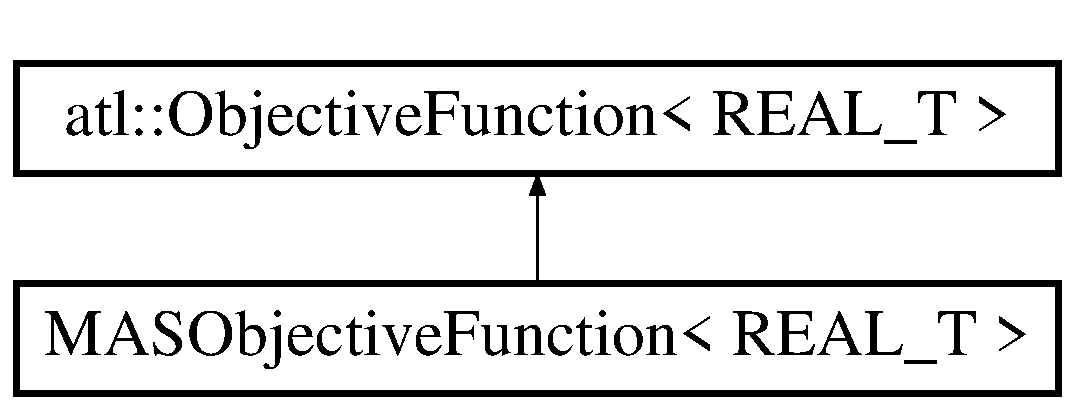
\includegraphics[height=2.000000cm]{class_m_a_s_objective_function}
\end{center}
\end{figure}
\subsection*{Public Types}
\begin{DoxyCompactItemize}
\item 
typedef \hyperlink{structmas_1_1_variable_trait}{mas\-::\-Variable\-Trait}\\*
$<$ R\-E\-A\-L\-\_\-\-T $>$\-::\hyperlink{class_m_a_s_objective_function_ab707ad68242cf26ada5f9fd8a0b077f8}{variable} \hyperlink{class_m_a_s_objective_function_ab707ad68242cf26ada5f9fd8a0b077f8}{variable}
\end{DoxyCompactItemize}
\subsection*{Public Member Functions}
\begin{DoxyCompactItemize}
\item 
virtual void \hyperlink{class_m_a_s_objective_function_a6c607be2d674fd2cb899d29a1c2892d3}{Initialize} ()
\item 
virtual void \hyperlink{class_m_a_s_objective_function_a17bdf39788f6f53b3b9b58e8c51735fd}{Finalize} ()
\item 
virtual void \hyperlink{class_m_a_s_objective_function_af3dc8db94367da71eaa2164ed8a7479b}{Output\-Var\-Covar} ()
\item 
virtual const atl\-::\-Variable\\*
$<$ R\-E\-A\-L\-\_\-\-T $>$ \hyperlink{class_m_a_s_objective_function_aa3bd6cce1fc71e640728f0c0a3876f99}{Evaluate} ()
\item 
virtual void \hyperlink{class_m_a_s_objective_function_ad1956703d67276fd3ddc9189d6e7f6f2}{Objective\-\_\-\-Function} (atl\-::\-Variable$<$ R\-E\-A\-L\-\_\-\-T $>$ \&f)
\end{DoxyCompactItemize}
\subsection*{Public Attributes}
\begin{DoxyCompactItemize}
\item 
\hyperlink{classmas_1_1_m_a_s}{mas\-::\-M\-A\-S}$<$ R\-E\-A\-L\-\_\-\-T $>$ \hyperlink{class_m_a_s_objective_function_acb7a8a71c46a7d51804cc8dd61bd558a}{mas}
\item 
std\-::string \hyperlink{class_m_a_s_objective_function_a829411b4be9bcb22e10e07748ef7b4f1}{data\-\_\-path} = \char`\"{}mas\-\_\-case\-\_\-1\-\_\-data.\-json\char`\"{}
\item 
std\-::string \hyperlink{class_m_a_s_objective_function_a2f79e227571b0ebbf941183aee8be623}{config\-\_\-path} = \char`\"{}mas\-\_\-cas31.\-json\char`\"{}
\end{DoxyCompactItemize}


\subsection{Detailed Description}
\subsubsection*{template$<$typename R\-E\-A\-L\-\_\-\-T$>$class M\-A\-S\-Objective\-Function$<$ R\-E\-A\-L\-\_\-\-T $>$}



Definition at line 26 of file main.\-cpp.



\subsection{Member Typedef Documentation}
\hypertarget{class_m_a_s_objective_function_ab707ad68242cf26ada5f9fd8a0b077f8}{\index{M\-A\-S\-Objective\-Function@{M\-A\-S\-Objective\-Function}!variable@{variable}}
\index{variable@{variable}!MASObjectiveFunction@{M\-A\-S\-Objective\-Function}}
\subsubsection[{variable}]{\setlength{\rightskip}{0pt plus 5cm}template$<$typename R\-E\-A\-L\-\_\-\-T$>$ typedef {\bf mas\-::\-Variable\-Trait}$<$R\-E\-A\-L\-\_\-\-T$>$\-::{\bf variable} {\bf M\-A\-S\-Objective\-Function}$<$ R\-E\-A\-L\-\_\-\-T $>$\-::{\bf variable}}}\label{class_m_a_s_objective_function_ab707ad68242cf26ada5f9fd8a0b077f8}


Definition at line 38 of file main.\-cpp.



\subsection{Member Function Documentation}
\hypertarget{class_m_a_s_objective_function_aa3bd6cce1fc71e640728f0c0a3876f99}{\index{M\-A\-S\-Objective\-Function@{M\-A\-S\-Objective\-Function}!Evaluate@{Evaluate}}
\index{Evaluate@{Evaluate}!MASObjectiveFunction@{M\-A\-S\-Objective\-Function}}
\subsubsection[{Evaluate}]{\setlength{\rightskip}{0pt plus 5cm}template$<$typename R\-E\-A\-L\-\_\-\-T$>$ virtual const atl\-::\-Variable$<$R\-E\-A\-L\-\_\-\-T$>$ {\bf M\-A\-S\-Objective\-Function}$<$ R\-E\-A\-L\-\_\-\-T $>$\-::Evaluate (
\begin{DoxyParamCaption}
{}
\end{DoxyParamCaption}
)\hspace{0.3cm}{\ttfamily [inline]}, {\ttfamily [virtual]}}}\label{class_m_a_s_objective_function_aa3bd6cce1fc71e640728f0c0a3876f99}


Definition at line 119 of file main.\-cpp.

\hypertarget{class_m_a_s_objective_function_a17bdf39788f6f53b3b9b58e8c51735fd}{\index{M\-A\-S\-Objective\-Function@{M\-A\-S\-Objective\-Function}!Finalize@{Finalize}}
\index{Finalize@{Finalize}!MASObjectiveFunction@{M\-A\-S\-Objective\-Function}}
\subsubsection[{Finalize}]{\setlength{\rightskip}{0pt plus 5cm}template$<$typename R\-E\-A\-L\-\_\-\-T$>$ virtual void {\bf M\-A\-S\-Objective\-Function}$<$ R\-E\-A\-L\-\_\-\-T $>$\-::Finalize (
\begin{DoxyParamCaption}
{}
\end{DoxyParamCaption}
)\hspace{0.3cm}{\ttfamily [inline]}, {\ttfamily [virtual]}}}\label{class_m_a_s_objective_function_a17bdf39788f6f53b3b9b58e8c51735fd}


Definition at line 48 of file main.\-cpp.

\hypertarget{class_m_a_s_objective_function_a6c607be2d674fd2cb899d29a1c2892d3}{\index{M\-A\-S\-Objective\-Function@{M\-A\-S\-Objective\-Function}!Initialize@{Initialize}}
\index{Initialize@{Initialize}!MASObjectiveFunction@{M\-A\-S\-Objective\-Function}}
\subsubsection[{Initialize}]{\setlength{\rightskip}{0pt plus 5cm}template$<$typename R\-E\-A\-L\-\_\-\-T$>$ virtual void {\bf M\-A\-S\-Objective\-Function}$<$ R\-E\-A\-L\-\_\-\-T $>$\-::Initialize (
\begin{DoxyParamCaption}
{}
\end{DoxyParamCaption}
)\hspace{0.3cm}{\ttfamily [inline]}, {\ttfamily [virtual]}}}\label{class_m_a_s_objective_function_a6c607be2d674fd2cb899d29a1c2892d3}


Definition at line 40 of file main.\-cpp.

\hypertarget{class_m_a_s_objective_function_ad1956703d67276fd3ddc9189d6e7f6f2}{\index{M\-A\-S\-Objective\-Function@{M\-A\-S\-Objective\-Function}!Objective\-\_\-\-Function@{Objective\-\_\-\-Function}}
\index{Objective\-\_\-\-Function@{Objective\-\_\-\-Function}!MASObjectiveFunction@{M\-A\-S\-Objective\-Function}}
\subsubsection[{Objective\-\_\-\-Function}]{\setlength{\rightskip}{0pt plus 5cm}template$<$typename R\-E\-A\-L\-\_\-\-T$>$ virtual void {\bf M\-A\-S\-Objective\-Function}$<$ R\-E\-A\-L\-\_\-\-T $>$\-::Objective\-\_\-\-Function (
\begin{DoxyParamCaption}
\item[{atl\-::\-Variable$<$ R\-E\-A\-L\-\_\-\-T $>$ \&}]{f}
\end{DoxyParamCaption}
)\hspace{0.3cm}{\ttfamily [inline]}, {\ttfamily [virtual]}}}\label{class_m_a_s_objective_function_ad1956703d67276fd3ddc9189d6e7f6f2}


Definition at line 126 of file main.\-cpp.

\hypertarget{class_m_a_s_objective_function_af3dc8db94367da71eaa2164ed8a7479b}{\index{M\-A\-S\-Objective\-Function@{M\-A\-S\-Objective\-Function}!Output\-Var\-Covar@{Output\-Var\-Covar}}
\index{Output\-Var\-Covar@{Output\-Var\-Covar}!MASObjectiveFunction@{M\-A\-S\-Objective\-Function}}
\subsubsection[{Output\-Var\-Covar}]{\setlength{\rightskip}{0pt plus 5cm}template$<$typename R\-E\-A\-L\-\_\-\-T$>$ virtual void {\bf M\-A\-S\-Objective\-Function}$<$ R\-E\-A\-L\-\_\-\-T $>$\-::Output\-Var\-Covar (
\begin{DoxyParamCaption}
{}
\end{DoxyParamCaption}
)\hspace{0.3cm}{\ttfamily [inline]}, {\ttfamily [virtual]}}}\label{class_m_a_s_objective_function_af3dc8db94367da71eaa2164ed8a7479b}


Definition at line 53 of file main.\-cpp.



\subsection{Member Data Documentation}
\hypertarget{class_m_a_s_objective_function_a2f79e227571b0ebbf941183aee8be623}{\index{M\-A\-S\-Objective\-Function@{M\-A\-S\-Objective\-Function}!config\-\_\-path@{config\-\_\-path}}
\index{config\-\_\-path@{config\-\_\-path}!MASObjectiveFunction@{M\-A\-S\-Objective\-Function}}
\subsubsection[{config\-\_\-path}]{\setlength{\rightskip}{0pt plus 5cm}template$<$typename R\-E\-A\-L\-\_\-\-T$>$ std\-::string {\bf M\-A\-S\-Objective\-Function}$<$ R\-E\-A\-L\-\_\-\-T $>$\-::config\-\_\-path = \char`\"{}mas\-\_\-cas31.\-json\char`\"{}}}\label{class_m_a_s_objective_function_a2f79e227571b0ebbf941183aee8be623}


Definition at line 35 of file main.\-cpp.

\hypertarget{class_m_a_s_objective_function_a829411b4be9bcb22e10e07748ef7b4f1}{\index{M\-A\-S\-Objective\-Function@{M\-A\-S\-Objective\-Function}!data\-\_\-path@{data\-\_\-path}}
\index{data\-\_\-path@{data\-\_\-path}!MASObjectiveFunction@{M\-A\-S\-Objective\-Function}}
\subsubsection[{data\-\_\-path}]{\setlength{\rightskip}{0pt plus 5cm}template$<$typename R\-E\-A\-L\-\_\-\-T$>$ std\-::string {\bf M\-A\-S\-Objective\-Function}$<$ R\-E\-A\-L\-\_\-\-T $>$\-::data\-\_\-path = \char`\"{}mas\-\_\-case\-\_\-1\-\_\-data.\-json\char`\"{}}}\label{class_m_a_s_objective_function_a829411b4be9bcb22e10e07748ef7b4f1}


Definition at line 33 of file main.\-cpp.

\hypertarget{class_m_a_s_objective_function_acb7a8a71c46a7d51804cc8dd61bd558a}{\index{M\-A\-S\-Objective\-Function@{M\-A\-S\-Objective\-Function}!mas@{mas}}
\index{mas@{mas}!MASObjectiveFunction@{M\-A\-S\-Objective\-Function}}
\subsubsection[{mas}]{\setlength{\rightskip}{0pt plus 5cm}template$<$typename R\-E\-A\-L\-\_\-\-T$>$ {\bf mas\-::\-M\-A\-S}$<$R\-E\-A\-L\-\_\-\-T$>$ {\bf M\-A\-S\-Objective\-Function}$<$ R\-E\-A\-L\-\_\-\-T $>$\-::mas}}\label{class_m_a_s_objective_function_acb7a8a71c46a7d51804cc8dd61bd558a}


Definition at line 29 of file main.\-cpp.



The documentation for this class was generated from the following file\-:\begin{DoxyCompactItemize}
\item 
/home/oppy/\-Net\-Beans\-Projects/mas/\hyperlink{main_8cpp}{main.\-cpp}\end{DoxyCompactItemize}

\hypertarget{structmas_1_1_model_object}{\section{mas\-:\-:Model\-Object$<$ R\-E\-A\-L\-\_\-\-T $>$ Struct Template Reference}
\label{structmas_1_1_model_object}\index{mas\-::\-Model\-Object$<$ R\-E\-A\-L\-\_\-\-T $>$@{mas\-::\-Model\-Object$<$ R\-E\-A\-L\-\_\-\-T $>$}}
}


{\ttfamily \#include $<$Common.\-hpp$>$}

Inheritance diagram for mas\-:\-:Model\-Object$<$ R\-E\-A\-L\-\_\-\-T $>$\-:\begin{figure}[H]
\begin{center}
\leavevmode
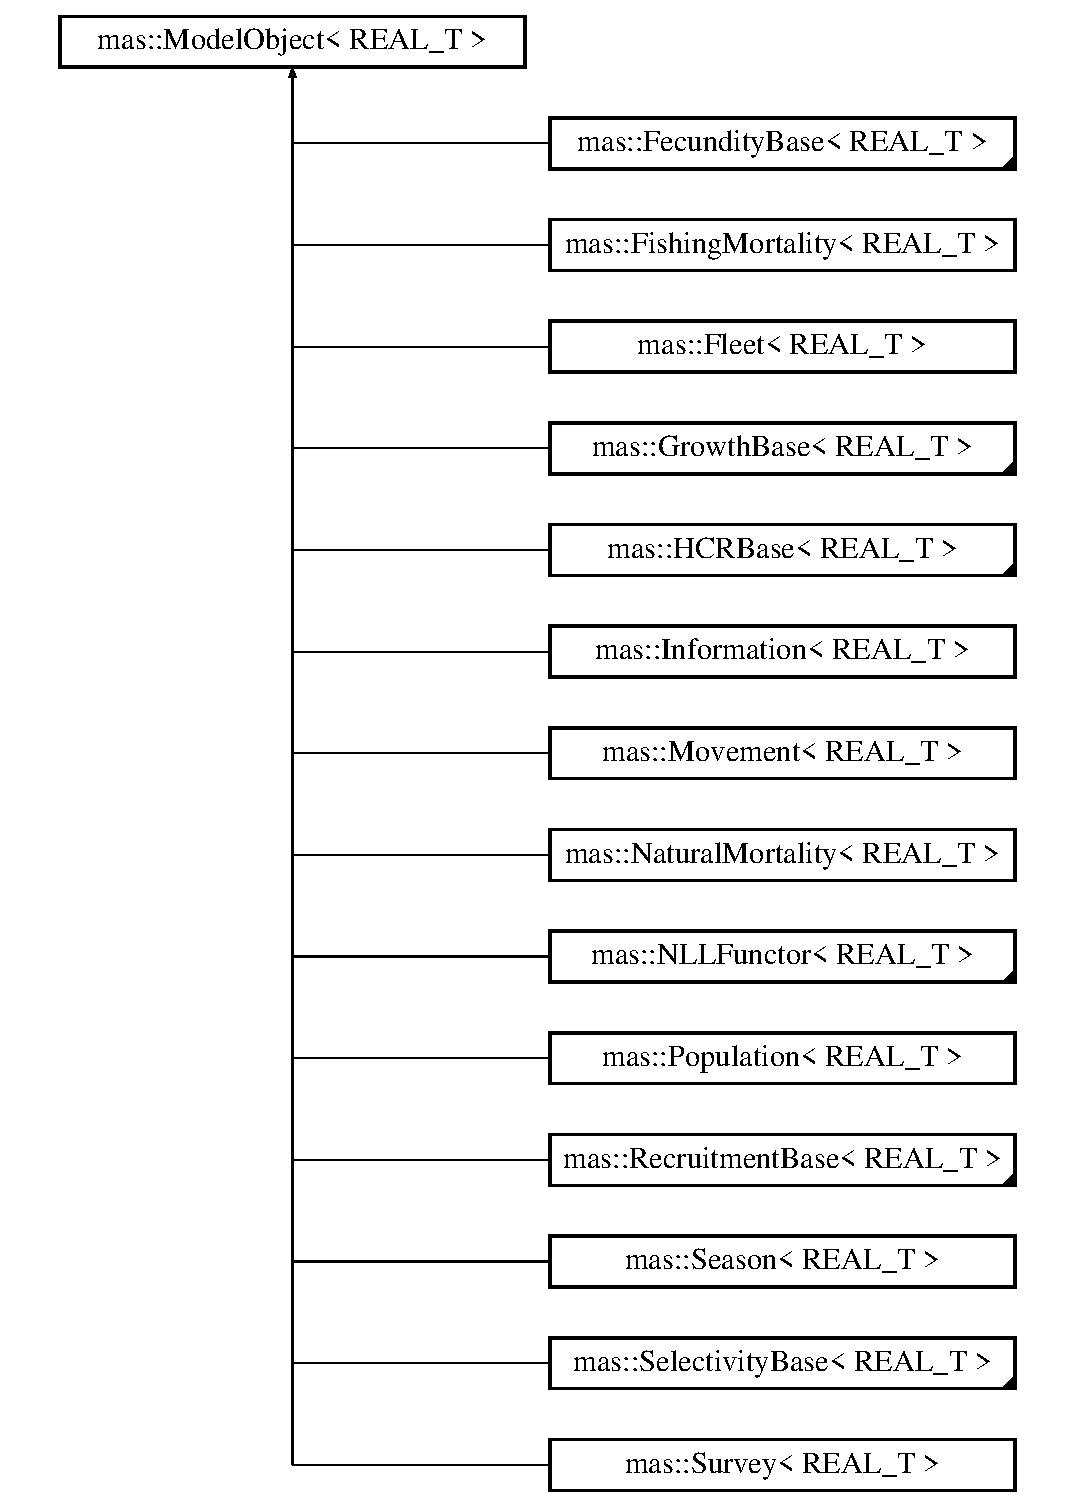
\includegraphics[height=12.000000cm]{structmas_1_1_model_object}
\end{center}
\end{figure}
\subsection*{Public Types}
\begin{DoxyCompactItemize}
\item 
typedef \hyperlink{structmas_1_1_variable_trait}{Variable\-Trait}$<$ R\-E\-A\-L\-\_\-\-T $>$\\*
\-::\hyperlink{structmas_1_1_model_object_a4e62fdbb5826f8fac311262b888ab10a}{variable} \hyperlink{structmas_1_1_model_object_a4e62fdbb5826f8fac311262b888ab10a}{variable}
\item 
typedef std\-::map$<$ \hyperlink{structmas_1_1_model_object_a4e62fdbb5826f8fac311262b888ab10a}{variable} \\*
$\ast$, int $>$\-::iterator \hyperlink{structmas_1_1_model_object_af95a47b3862d83583751c2d835887697}{estimable\-\_\-parameter\-\_\-iterator}
\end{DoxyCompactItemize}
\subsection*{Public Member Functions}
\begin{DoxyCompactItemize}
\item 
void \hyperlink{structmas_1_1_model_object_aefad28a4f78daee1ead3eaa0a44577ae}{Register} (\hyperlink{structmas_1_1_model_object_a4e62fdbb5826f8fac311262b888ab10a}{variable} \&var, int phase=1)
\item 
virtual const std\-::string \hyperlink{structmas_1_1_model_object_a68948da33f7370cfea0f07bbe072a439}{J\-S\-O\-N\-Parameter} (\hyperlink{structmas_1_1_model_object_a4e62fdbb5826f8fac311262b888ab10a}{variable} \&var, const std\-::string \&name)
\item 
virtual const std\-::string \hyperlink{structmas_1_1_model_object_af40b3c89b11919fc5aea21dcf1cd027b}{To\-J\-S\-O\-N\-String} ()
\item 
virtual std\-::string \hyperlink{structmas_1_1_model_object_a8eaf6c7c52e42ea8869aefa318358cb5}{To\-String} ()
\end{DoxyCompactItemize}
\subsection*{Public Attributes}
\begin{DoxyCompactItemize}
\item 
int \hyperlink{structmas_1_1_model_object_a1455cdfd12f282766b0689f3a345dbb7}{id}
\item 
std\-::map$<$ \hyperlink{structmas_1_1_model_object_a4e62fdbb5826f8fac311262b888ab10a}{variable} $\ast$, int $>$ \hyperlink{structmas_1_1_model_object_aaea24720c307701c6c4494088013cc46}{estimated\-\_\-parameters\-\_\-map}
\item 
std\-::vector$<$ \hyperlink{structmas_1_1_model_object_a4e62fdbb5826f8fac311262b888ab10a}{variable} $\ast$ $>$ \hyperlink{structmas_1_1_model_object_ae9b9d70e413f78bf9b566eba16d1e71c}{estimated\-\_\-parameters}
\item 
std\-::vector$<$ int $>$ \hyperlink{structmas_1_1_model_object_a6e26b63869a25bbe17a8d57e4d4ab77a}{estimated\-\_\-phase}
\item 
bool \hyperlink{structmas_1_1_model_object_a47d30dfc08290aebd94cf3096d53ef6a}{used} = false
\end{DoxyCompactItemize}


\subsection{Detailed Description}
\subsubsection*{template$<$typename R\-E\-A\-L\-\_\-\-T$>$struct mas\-::\-Model\-Object$<$ R\-E\-A\-L\-\_\-\-T $>$}



Definition at line 50 of file Common.\-hpp.



\subsection{Member Typedef Documentation}
\hypertarget{structmas_1_1_model_object_af95a47b3862d83583751c2d835887697}{\index{mas\-::\-Model\-Object@{mas\-::\-Model\-Object}!estimable\-\_\-parameter\-\_\-iterator@{estimable\-\_\-parameter\-\_\-iterator}}
\index{estimable\-\_\-parameter\-\_\-iterator@{estimable\-\_\-parameter\-\_\-iterator}!mas::ModelObject@{mas\-::\-Model\-Object}}
\subsubsection[{estimable\-\_\-parameter\-\_\-iterator}]{\setlength{\rightskip}{0pt plus 5cm}template$<$typename R\-E\-A\-L\-\_\-\-T$>$ typedef std\-::map$<${\bf variable}$\ast$, int$>$\-::iterator {\bf mas\-::\-Model\-Object}$<$ R\-E\-A\-L\-\_\-\-T $>$\-::{\bf estimable\-\_\-parameter\-\_\-iterator}}}\label{structmas_1_1_model_object_af95a47b3862d83583751c2d835887697}


Definition at line 54 of file Common.\-hpp.

\hypertarget{structmas_1_1_model_object_a4e62fdbb5826f8fac311262b888ab10a}{\index{mas\-::\-Model\-Object@{mas\-::\-Model\-Object}!variable@{variable}}
\index{variable@{variable}!mas::ModelObject@{mas\-::\-Model\-Object}}
\subsubsection[{variable}]{\setlength{\rightskip}{0pt plus 5cm}template$<$typename R\-E\-A\-L\-\_\-\-T$>$ typedef {\bf Variable\-Trait}$<$R\-E\-A\-L\-\_\-\-T$>$\-::{\bf variable} {\bf mas\-::\-Model\-Object}$<$ R\-E\-A\-L\-\_\-\-T $>$\-::{\bf variable}}}\label{structmas_1_1_model_object_a4e62fdbb5826f8fac311262b888ab10a}


Definition at line 51 of file Common.\-hpp.



\subsection{Member Function Documentation}
\hypertarget{structmas_1_1_model_object_a68948da33f7370cfea0f07bbe072a439}{\index{mas\-::\-Model\-Object@{mas\-::\-Model\-Object}!J\-S\-O\-N\-Parameter@{J\-S\-O\-N\-Parameter}}
\index{J\-S\-O\-N\-Parameter@{J\-S\-O\-N\-Parameter}!mas::ModelObject@{mas\-::\-Model\-Object}}
\subsubsection[{J\-S\-O\-N\-Parameter}]{\setlength{\rightskip}{0pt plus 5cm}template$<$typename R\-E\-A\-L\-\_\-\-T$>$ virtual const std\-::string {\bf mas\-::\-Model\-Object}$<$ R\-E\-A\-L\-\_\-\-T $>$\-::J\-S\-O\-N\-Parameter (
\begin{DoxyParamCaption}
\item[{{\bf variable} \&}]{var, }
\item[{const std\-::string \&}]{name}
\end{DoxyParamCaption}
)\hspace{0.3cm}{\ttfamily [inline]}, {\ttfamily [virtual]}}}\label{structmas_1_1_model_object_a68948da33f7370cfea0f07bbe072a439}


Definition at line 65 of file Common.\-hpp.

\hypertarget{structmas_1_1_model_object_aefad28a4f78daee1ead3eaa0a44577ae}{\index{mas\-::\-Model\-Object@{mas\-::\-Model\-Object}!Register@{Register}}
\index{Register@{Register}!mas::ModelObject@{mas\-::\-Model\-Object}}
\subsubsection[{Register}]{\setlength{\rightskip}{0pt plus 5cm}template$<$typename R\-E\-A\-L\-\_\-\-T$>$ void {\bf mas\-::\-Model\-Object}$<$ R\-E\-A\-L\-\_\-\-T $>$\-::Register (
\begin{DoxyParamCaption}
\item[{{\bf variable} \&}]{var, }
\item[{int}]{phase = {\ttfamily 1}}
\end{DoxyParamCaption}
)\hspace{0.3cm}{\ttfamily [inline]}}}\label{structmas_1_1_model_object_aefad28a4f78daee1ead3eaa0a44577ae}


Definition at line 59 of file Common.\-hpp.

\hypertarget{structmas_1_1_model_object_af40b3c89b11919fc5aea21dcf1cd027b}{\index{mas\-::\-Model\-Object@{mas\-::\-Model\-Object}!To\-J\-S\-O\-N\-String@{To\-J\-S\-O\-N\-String}}
\index{To\-J\-S\-O\-N\-String@{To\-J\-S\-O\-N\-String}!mas::ModelObject@{mas\-::\-Model\-Object}}
\subsubsection[{To\-J\-S\-O\-N\-String}]{\setlength{\rightskip}{0pt plus 5cm}template$<$typename R\-E\-A\-L\-\_\-\-T$>$ virtual const std\-::string {\bf mas\-::\-Model\-Object}$<$ R\-E\-A\-L\-\_\-\-T $>$\-::To\-J\-S\-O\-N\-String (
\begin{DoxyParamCaption}
{}
\end{DoxyParamCaption}
)\hspace{0.3cm}{\ttfamily [inline]}, {\ttfamily [virtual]}}}\label{structmas_1_1_model_object_af40b3c89b11919fc5aea21dcf1cd027b}


Reimplemented in \hyperlink{classmas_1_1_population_adb6e6afabb8a27f64592f36909d43612}{mas\-::\-Population$<$ R\-E\-A\-L\-\_\-\-T $>$}, \hyperlink{structmas_1_1_fleet_a438089d58f104668621d9426fa1e1c86}{mas\-::\-Fleet$<$ R\-E\-A\-L\-\_\-\-T $>$}, \hyperlink{structmas_1_1_deriso_aabf1cedad5697f1924a09d3a168453c4}{mas\-::\-Deriso$<$ R\-E\-A\-L\-\_\-\-T $>$}, \hyperlink{structmas_1_1_schnute_case_i_v_a1f6dc0866ead488d7258b75193305c9b}{mas\-::\-Schnute\-Case\-I\-V$<$ R\-E\-A\-L\-\_\-\-T $>$}, \hyperlink{structmas_1_1_shepherd_aafe14075a992d9157bc8594aac0a2eeb}{mas\-::\-Shepherd$<$ R\-E\-A\-L\-\_\-\-T $>$}, \hyperlink{structmas_1_1_schnute_case_i_i_i_a7f55a0a6f9f4f8f577c952ec974c89c4}{mas\-::\-Schnute\-Case\-I\-I\-I$<$ R\-E\-A\-L\-\_\-\-T $>$}, \hyperlink{structmas_1_1_inverse_quadratic_r_b_f_a59195ed8bba6ab30d34fa1d204c264bf}{mas\-::\-Inverse\-Quadratic\-R\-B\-F$<$ R\-E\-A\-L\-\_\-\-T $>$}, \hyperlink{structmas_1_1_beverton_holt_dep_ac2af0de80fd4cc3606d8986cfa1e5781}{mas\-::\-Beverton\-Holt\-Dep$<$ R\-E\-A\-L\-\_\-\-T $>$}, \hyperlink{structmas_1_1_schnute_case_i_i_a291cd832a760d0a08e838fd251f98b2b}{mas\-::\-Schnute\-Case\-I\-I$<$ R\-E\-A\-L\-\_\-\-T $>$}, \hyperlink{structmas_1_1_beverton_holt_alt_ae81da66f21c345daabf90fc7aa0db6c7}{mas\-::\-Beverton\-Holt\-Alt$<$ R\-E\-A\-L\-\_\-\-T $>$}, \hyperlink{structmas_1_1_gaussian_r_b_f_a0b07e709655b2c7da7c89dd48491d091}{mas\-::\-Gaussian\-R\-B\-F$<$ R\-E\-A\-L\-\_\-\-T $>$}, \hyperlink{structmas_1_1_schnute_case_i_a84e734071e4bf0cce1d36c00f94768db}{mas\-::\-Schnute\-Case\-I$<$ R\-E\-A\-L\-\_\-\-T $>$}, \hyperlink{structmas_1_1_beverton_holt_a273d2704a4974d3fdbb9287ad0984b69}{mas\-::\-Beverton\-Holt$<$ R\-E\-A\-L\-\_\-\-T $>$}, \hyperlink{structmas_1_1_fishing_mortality_ac76d1e34d6c062d090bc5265d100395d}{mas\-::\-Fishing\-Mortality$<$ R\-E\-A\-L\-\_\-\-T $>$}, \hyperlink{structmas_1_1_ricker_alt_a76187fc316998d57d245c189560bcade}{mas\-::\-Ricker\-Alt$<$ R\-E\-A\-L\-\_\-\-T $>$}, \hyperlink{structmas_1_1_von_bertalanffy_modified_a47465618fc2471ad0f47f94fe3974597}{mas\-::\-Von\-Bertalanffy\-Modified$<$ R\-E\-A\-L\-\_\-\-T $>$}, \hyperlink{structmas_1_1_double_logistic_sel_af25cc89b1ae6e3b53774c59b8b440699}{mas\-::\-Double\-Logistic\-Sel$<$ R\-E\-A\-L\-\_\-\-T $>$}, \hyperlink{structmas_1_1_ricker_af6cb56b70e0449cfb5fdfab757971560}{mas\-::\-Ricker$<$ R\-E\-A\-L\-\_\-\-T $>$}, \hyperlink{structmas_1_1_von_bertalanffy_a1b579d133d8f9d068afec3b3a386ceec}{mas\-::\-Von\-Bertalanffy$<$ R\-E\-A\-L\-\_\-\-T $>$}, \hyperlink{structmas_1_1_logistic_sel_afa9abd8671cf8d82a6973c4369741b41}{mas\-::\-Logistic\-Sel$<$ R\-E\-A\-L\-\_\-\-T $>$}, \hyperlink{structmas_1_1_movement_a6ace5dba1349ee6fde5c242a467155d4}{mas\-::\-Movement$<$ R\-E\-A\-L\-\_\-\-T $>$}, and \hyperlink{structmas_1_1_natural_mortality_ae788facfc8178ed04eeb1d31caada8f3}{mas\-::\-Natural\-Mortality$<$ R\-E\-A\-L\-\_\-\-T $>$}.



Definition at line 87 of file Common.\-hpp.

\hypertarget{structmas_1_1_model_object_a8eaf6c7c52e42ea8869aefa318358cb5}{\index{mas\-::\-Model\-Object@{mas\-::\-Model\-Object}!To\-String@{To\-String}}
\index{To\-String@{To\-String}!mas::ModelObject@{mas\-::\-Model\-Object}}
\subsubsection[{To\-String}]{\setlength{\rightskip}{0pt plus 5cm}template$<$typename R\-E\-A\-L\-\_\-\-T$>$ virtual std\-::string {\bf mas\-::\-Model\-Object}$<$ R\-E\-A\-L\-\_\-\-T $>$\-::To\-String (
\begin{DoxyParamCaption}
{}
\end{DoxyParamCaption}
)\hspace{0.3cm}{\ttfamily [inline]}, {\ttfamily [virtual]}}}\label{structmas_1_1_model_object_a8eaf6c7c52e42ea8869aefa318358cb5}


Reimplemented in \hyperlink{structmas_1_1_multinomial_robust_a57b1509abe3c1640fb0e24f636fbbd87}{mas\-::\-Multinomial\-Robust$<$ R\-E\-A\-L\-\_\-\-T $>$}, \hyperlink{structmas_1_1_schnute_case_i_v_ac95b913d4a28421b37e8c91e76906f2d}{mas\-::\-Schnute\-Case\-I\-V$<$ R\-E\-A\-L\-\_\-\-T $>$}, \hyperlink{structmas_1_1_multinomial_a90903904b06f2e5a79ffba4981fef34a}{mas\-::\-Multinomial$<$ R\-E\-A\-L\-\_\-\-T $>$}, \hyperlink{structmas_1_1_schnute_case_i_i_i_af99d1855589bc44641952cfc89d11a72}{mas\-::\-Schnute\-Case\-I\-I\-I$<$ R\-E\-A\-L\-\_\-\-T $>$}, \hyperlink{structmas_1_1_inverse_quadratic_r_b_f_a51999c40500b4bedc5bb24a1b0b87bb7}{mas\-::\-Inverse\-Quadratic\-R\-B\-F$<$ R\-E\-A\-L\-\_\-\-T $>$}, \hyperlink{structmas_1_1_dirichlet_multinomial_robust_a25f3b78a3072162c8e1fce217a599a14}{mas\-::\-Dirichlet\-Multinomial\-Robust$<$ R\-E\-A\-L\-\_\-\-T $>$}, \hyperlink{structmas_1_1_schnute_case_i_i_ac4cca4d5d808023e1a72651ea090fc58}{mas\-::\-Schnute\-Case\-I\-I$<$ R\-E\-A\-L\-\_\-\-T $>$}, \hyperlink{structmas_1_1_gaussian_r_b_f_a08856503cb0e77c17f891621aef50d21}{mas\-::\-Gaussian\-R\-B\-F$<$ R\-E\-A\-L\-\_\-\-T $>$}, \hyperlink{structmas_1_1_schnute_case_i_a75bd8ce2e0224680c775a70122f18232}{mas\-::\-Schnute\-Case\-I$<$ R\-E\-A\-L\-\_\-\-T $>$}, \hyperlink{structmas_1_1_dirichlet_multinomial_a92d0abed181db2f54d7d44ac7cb4fa27}{mas\-::\-Dirichlet\-Multinomial$<$ R\-E\-A\-L\-\_\-\-T $>$}, \hyperlink{structmas_1_1_von_bertalanffy_modified_a45e40092ed15953212d65c406908d708}{mas\-::\-Von\-Bertalanffy\-Modified$<$ R\-E\-A\-L\-\_\-\-T $>$}, \hyperlink{structmas_1_1_n_l_l_functor_accd55442e1e88b423471b67c40860197}{mas\-::\-N\-L\-L\-Functor$<$ R\-E\-A\-L\-\_\-\-T $>$}, \hyperlink{structmas_1_1_double_logistic_sel_ab91353c57277a40f04c505ce77332c65}{mas\-::\-Double\-Logistic\-Sel$<$ R\-E\-A\-L\-\_\-\-T $>$}, \hyperlink{structmas_1_1_fishing_mortality_a584a63c9d45ec427965f2d98c2a88c81}{mas\-::\-Fishing\-Mortality$<$ R\-E\-A\-L\-\_\-\-T $>$}, \hyperlink{structmas_1_1_von_bertalanffy_af301e548d6d3e9df5a2fc65132378195}{mas\-::\-Von\-Bertalanffy$<$ R\-E\-A\-L\-\_\-\-T $>$}, and \hyperlink{structmas_1_1_logistic_sel_a625cc43faa89094c25da029a827ba638}{mas\-::\-Logistic\-Sel$<$ R\-E\-A\-L\-\_\-\-T $>$}.



Definition at line 91 of file Common.\-hpp.



\subsection{Member Data Documentation}
\hypertarget{structmas_1_1_model_object_ae9b9d70e413f78bf9b566eba16d1e71c}{\index{mas\-::\-Model\-Object@{mas\-::\-Model\-Object}!estimated\-\_\-parameters@{estimated\-\_\-parameters}}
\index{estimated\-\_\-parameters@{estimated\-\_\-parameters}!mas::ModelObject@{mas\-::\-Model\-Object}}
\subsubsection[{estimated\-\_\-parameters}]{\setlength{\rightskip}{0pt plus 5cm}template$<$typename R\-E\-A\-L\-\_\-\-T$>$ std\-::vector$<${\bf variable}$\ast$$>$ {\bf mas\-::\-Model\-Object}$<$ R\-E\-A\-L\-\_\-\-T $>$\-::estimated\-\_\-parameters}}\label{structmas_1_1_model_object_ae9b9d70e413f78bf9b566eba16d1e71c}


Definition at line 55 of file Common.\-hpp.

\hypertarget{structmas_1_1_model_object_aaea24720c307701c6c4494088013cc46}{\index{mas\-::\-Model\-Object@{mas\-::\-Model\-Object}!estimated\-\_\-parameters\-\_\-map@{estimated\-\_\-parameters\-\_\-map}}
\index{estimated\-\_\-parameters\-\_\-map@{estimated\-\_\-parameters\-\_\-map}!mas::ModelObject@{mas\-::\-Model\-Object}}
\subsubsection[{estimated\-\_\-parameters\-\_\-map}]{\setlength{\rightskip}{0pt plus 5cm}template$<$typename R\-E\-A\-L\-\_\-\-T$>$ std\-::map$<${\bf variable}$\ast$, int$>$ {\bf mas\-::\-Model\-Object}$<$ R\-E\-A\-L\-\_\-\-T $>$\-::estimated\-\_\-parameters\-\_\-map}}\label{structmas_1_1_model_object_aaea24720c307701c6c4494088013cc46}


Definition at line 53 of file Common.\-hpp.

\hypertarget{structmas_1_1_model_object_a6e26b63869a25bbe17a8d57e4d4ab77a}{\index{mas\-::\-Model\-Object@{mas\-::\-Model\-Object}!estimated\-\_\-phase@{estimated\-\_\-phase}}
\index{estimated\-\_\-phase@{estimated\-\_\-phase}!mas::ModelObject@{mas\-::\-Model\-Object}}
\subsubsection[{estimated\-\_\-phase}]{\setlength{\rightskip}{0pt plus 5cm}template$<$typename R\-E\-A\-L\-\_\-\-T$>$ std\-::vector$<$int$>$ {\bf mas\-::\-Model\-Object}$<$ R\-E\-A\-L\-\_\-\-T $>$\-::estimated\-\_\-phase}}\label{structmas_1_1_model_object_a6e26b63869a25bbe17a8d57e4d4ab77a}


Definition at line 56 of file Common.\-hpp.

\hypertarget{structmas_1_1_model_object_a1455cdfd12f282766b0689f3a345dbb7}{\index{mas\-::\-Model\-Object@{mas\-::\-Model\-Object}!id@{id}}
\index{id@{id}!mas::ModelObject@{mas\-::\-Model\-Object}}
\subsubsection[{id}]{\setlength{\rightskip}{0pt plus 5cm}template$<$typename R\-E\-A\-L\-\_\-\-T$>$ int {\bf mas\-::\-Model\-Object}$<$ R\-E\-A\-L\-\_\-\-T $>$\-::id}}\label{structmas_1_1_model_object_a1455cdfd12f282766b0689f3a345dbb7}


Definition at line 52 of file Common.\-hpp.

\hypertarget{structmas_1_1_model_object_a47d30dfc08290aebd94cf3096d53ef6a}{\index{mas\-::\-Model\-Object@{mas\-::\-Model\-Object}!used@{used}}
\index{used@{used}!mas::ModelObject@{mas\-::\-Model\-Object}}
\subsubsection[{used}]{\setlength{\rightskip}{0pt plus 5cm}template$<$typename R\-E\-A\-L\-\_\-\-T$>$ bool {\bf mas\-::\-Model\-Object}$<$ R\-E\-A\-L\-\_\-\-T $>$\-::used = false}}\label{structmas_1_1_model_object_a47d30dfc08290aebd94cf3096d53ef6a}


Definition at line 57 of file Common.\-hpp.



The documentation for this struct was generated from the following file\-:\begin{DoxyCompactItemize}
\item 
/home/oppy/\-Net\-Beans\-Projects/mas/\hyperlink{_common_8hpp}{Common.\-hpp}\end{DoxyCompactItemize}

\hypertarget{structmas_1_1_movement}{\section{mas\-:\-:Movement$<$ R\-E\-A\-L\-\_\-\-T $>$ Struct Template Reference}
\label{structmas_1_1_movement}\index{mas\-::\-Movement$<$ R\-E\-A\-L\-\_\-\-T $>$@{mas\-::\-Movement$<$ R\-E\-A\-L\-\_\-\-T $>$}}
}


{\ttfamily \#include $<$Movement.\-hpp$>$}

Inheritance diagram for mas\-:\-:Movement$<$ R\-E\-A\-L\-\_\-\-T $>$\-:\begin{figure}[H]
\begin{center}
\leavevmode
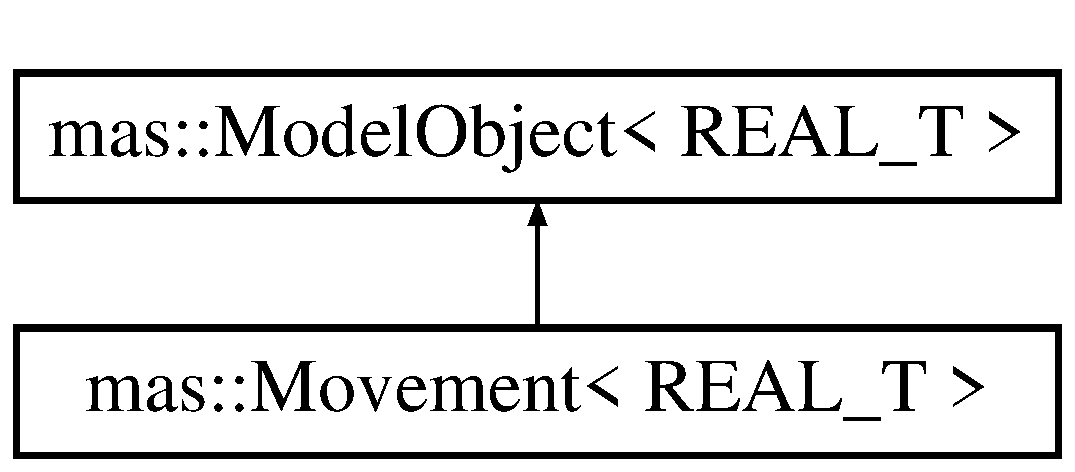
\includegraphics[height=2.000000cm]{structmas_1_1_movement}
\end{center}
\end{figure}
\subsection*{Public Types}
\begin{DoxyCompactItemize}
\item 
typedef \hyperlink{structmas_1_1_variable_trait}{Variable\-Trait}$<$ R\-E\-A\-L\-\_\-\-T $>$\\*
\-::\hyperlink{structmas_1_1_movement_a4667a4bb2ad370d0cf6b476eb625288e}{variable} \hyperlink{structmas_1_1_movement_a4667a4bb2ad370d0cf6b476eb625288e}{variable}
\end{DoxyCompactItemize}
\subsection*{Public Member Functions}
\begin{DoxyCompactItemize}
\item 
virtual const std\-::string \hyperlink{structmas_1_1_movement_a59f6870b613e273f4d5521beb5710d88}{Name} ()
\item 
virtual const std\-::string \hyperlink{structmas_1_1_movement_a6ace5dba1349ee6fde5c242a467155d4}{To\-J\-S\-O\-N\-String} ()
\end{DoxyCompactItemize}
\subsection*{Public Attributes}
\begin{DoxyCompactItemize}
\item 
std\-::vector$<$ std\-::vector\\*
$<$ std\-::vector$<$ \hyperlink{structmas_1_1_movement_a4667a4bb2ad370d0cf6b476eb625288e}{variable} $>$ $>$ $>$ \hyperlink{structmas_1_1_movement_a07f5b43bad4f99ee026a0b8d3d354049}{recruit\-\_\-connectivity}
\item 
std\-::vector$<$ std\-::vector\\*
$<$ std\-::vector$<$ \hyperlink{structmas_1_1_movement_a4667a4bb2ad370d0cf6b476eb625288e}{variable} $>$ $>$ $>$ \hyperlink{structmas_1_1_movement_aa48b8bad16dfcbca315467a7a7c6ea95}{male\-\_\-connectivity}
\item 
std\-::vector$<$ std\-::vector\\*
$<$ std\-::vector$<$ \hyperlink{structmas_1_1_movement_a4667a4bb2ad370d0cf6b476eb625288e}{variable} $>$ $>$ $>$ \hyperlink{structmas_1_1_movement_a5425a809307c33799cd4c0fee06d54f1}{female\-\_\-connectivity}
\end{DoxyCompactItemize}


\subsection{Detailed Description}
\subsubsection*{template$<$typename R\-E\-A\-L\-\_\-\-T$>$struct mas\-::\-Movement$<$ R\-E\-A\-L\-\_\-\-T $>$}

\hyperlink{structmas_1_1_movement}{Movement} probabilities for a box-\/transfer model for a given year.

Probability information is defined by season and areas. 

Definition at line 46 of file Movement.\-hpp.



\subsection{Member Typedef Documentation}
\hypertarget{structmas_1_1_movement_a4667a4bb2ad370d0cf6b476eb625288e}{\index{mas\-::\-Movement@{mas\-::\-Movement}!variable@{variable}}
\index{variable@{variable}!mas::Movement@{mas\-::\-Movement}}
\subsubsection[{variable}]{\setlength{\rightskip}{0pt plus 5cm}template$<$typename R\-E\-A\-L\-\_\-\-T $>$ typedef {\bf Variable\-Trait}$<$R\-E\-A\-L\-\_\-\-T$>$\-::{\bf variable} {\bf mas\-::\-Movement}$<$ R\-E\-A\-L\-\_\-\-T $>$\-::{\bf variable}}}\label{structmas_1_1_movement_a4667a4bb2ad370d0cf6b476eb625288e}


Definition at line 47 of file Movement.\-hpp.



\subsection{Member Function Documentation}
\hypertarget{structmas_1_1_movement_a59f6870b613e273f4d5521beb5710d88}{\index{mas\-::\-Movement@{mas\-::\-Movement}!Name@{Name}}
\index{Name@{Name}!mas::Movement@{mas\-::\-Movement}}
\subsubsection[{Name}]{\setlength{\rightskip}{0pt plus 5cm}template$<$typename R\-E\-A\-L\-\_\-\-T $>$ virtual const std\-::string {\bf mas\-::\-Movement}$<$ R\-E\-A\-L\-\_\-\-T $>$\-::Name (
\begin{DoxyParamCaption}
{}
\end{DoxyParamCaption}
)\hspace{0.3cm}{\ttfamily [inline]}, {\ttfamily [virtual]}}}\label{structmas_1_1_movement_a59f6870b613e273f4d5521beb5710d88}


Definition at line 52 of file Movement.\-hpp.

\hypertarget{structmas_1_1_movement_a6ace5dba1349ee6fde5c242a467155d4}{\index{mas\-::\-Movement@{mas\-::\-Movement}!To\-J\-S\-O\-N\-String@{To\-J\-S\-O\-N\-String}}
\index{To\-J\-S\-O\-N\-String@{To\-J\-S\-O\-N\-String}!mas::Movement@{mas\-::\-Movement}}
\subsubsection[{To\-J\-S\-O\-N\-String}]{\setlength{\rightskip}{0pt plus 5cm}template$<$typename R\-E\-A\-L\-\_\-\-T $>$ virtual const std\-::string {\bf mas\-::\-Movement}$<$ R\-E\-A\-L\-\_\-\-T $>$\-::To\-J\-S\-O\-N\-String (
\begin{DoxyParamCaption}
{}
\end{DoxyParamCaption}
)\hspace{0.3cm}{\ttfamily [inline]}, {\ttfamily [virtual]}}}\label{structmas_1_1_movement_a6ace5dba1349ee6fde5c242a467155d4}


Reimplemented from \hyperlink{structmas_1_1_model_object_af40b3c89b11919fc5aea21dcf1cd027b}{mas\-::\-Model\-Object$<$ R\-E\-A\-L\-\_\-\-T $>$}.



Definition at line 56 of file Movement.\-hpp.



\subsection{Member Data Documentation}
\hypertarget{structmas_1_1_movement_a5425a809307c33799cd4c0fee06d54f1}{\index{mas\-::\-Movement@{mas\-::\-Movement}!female\-\_\-connectivity@{female\-\_\-connectivity}}
\index{female\-\_\-connectivity@{female\-\_\-connectivity}!mas::Movement@{mas\-::\-Movement}}
\subsubsection[{female\-\_\-connectivity}]{\setlength{\rightskip}{0pt plus 5cm}template$<$typename R\-E\-A\-L\-\_\-\-T $>$ std\-::vector$<$std\-::vector$<$std\-::vector$<${\bf variable}$>$ $>$ $>$ {\bf mas\-::\-Movement}$<$ R\-E\-A\-L\-\_\-\-T $>$\-::female\-\_\-connectivity}}\label{structmas_1_1_movement_a5425a809307c33799cd4c0fee06d54f1}


Definition at line 50 of file Movement.\-hpp.

\hypertarget{structmas_1_1_movement_aa48b8bad16dfcbca315467a7a7c6ea95}{\index{mas\-::\-Movement@{mas\-::\-Movement}!male\-\_\-connectivity@{male\-\_\-connectivity}}
\index{male\-\_\-connectivity@{male\-\_\-connectivity}!mas::Movement@{mas\-::\-Movement}}
\subsubsection[{male\-\_\-connectivity}]{\setlength{\rightskip}{0pt plus 5cm}template$<$typename R\-E\-A\-L\-\_\-\-T $>$ std\-::vector$<$std\-::vector$<$std\-::vector$<${\bf variable}$>$ $>$ $>$ {\bf mas\-::\-Movement}$<$ R\-E\-A\-L\-\_\-\-T $>$\-::male\-\_\-connectivity}}\label{structmas_1_1_movement_aa48b8bad16dfcbca315467a7a7c6ea95}


Definition at line 49 of file Movement.\-hpp.

\hypertarget{structmas_1_1_movement_a07f5b43bad4f99ee026a0b8d3d354049}{\index{mas\-::\-Movement@{mas\-::\-Movement}!recruit\-\_\-connectivity@{recruit\-\_\-connectivity}}
\index{recruit\-\_\-connectivity@{recruit\-\_\-connectivity}!mas::Movement@{mas\-::\-Movement}}
\subsubsection[{recruit\-\_\-connectivity}]{\setlength{\rightskip}{0pt plus 5cm}template$<$typename R\-E\-A\-L\-\_\-\-T $>$ std\-::vector$<$std\-::vector$<$std\-::vector$<${\bf variable}$>$ $>$ $>$ {\bf mas\-::\-Movement}$<$ R\-E\-A\-L\-\_\-\-T $>$\-::recruit\-\_\-connectivity}}\label{structmas_1_1_movement_a07f5b43bad4f99ee026a0b8d3d354049}


Definition at line 48 of file Movement.\-hpp.



The documentation for this struct was generated from the following file\-:\begin{DoxyCompactItemize}
\item 
/home/oppy/\-Net\-Beans\-Projects/mas/\hyperlink{_movement_8hpp}{Movement.\-hpp}\end{DoxyCompactItemize}

\hypertarget{structmas_1_1_multinomial}{\section{mas\-:\-:Multinomial$<$ R\-E\-A\-L\-\_\-\-T $>$ Struct Template Reference}
\label{structmas_1_1_multinomial}\index{mas\-::\-Multinomial$<$ R\-E\-A\-L\-\_\-\-T $>$@{mas\-::\-Multinomial$<$ R\-E\-A\-L\-\_\-\-T $>$}}
}


{\ttfamily \#include $<$N\-L\-L\-Components.\-hpp$>$}

Inheritance diagram for mas\-:\-:Multinomial$<$ R\-E\-A\-L\-\_\-\-T $>$\-:\begin{figure}[H]
\begin{center}
\leavevmode
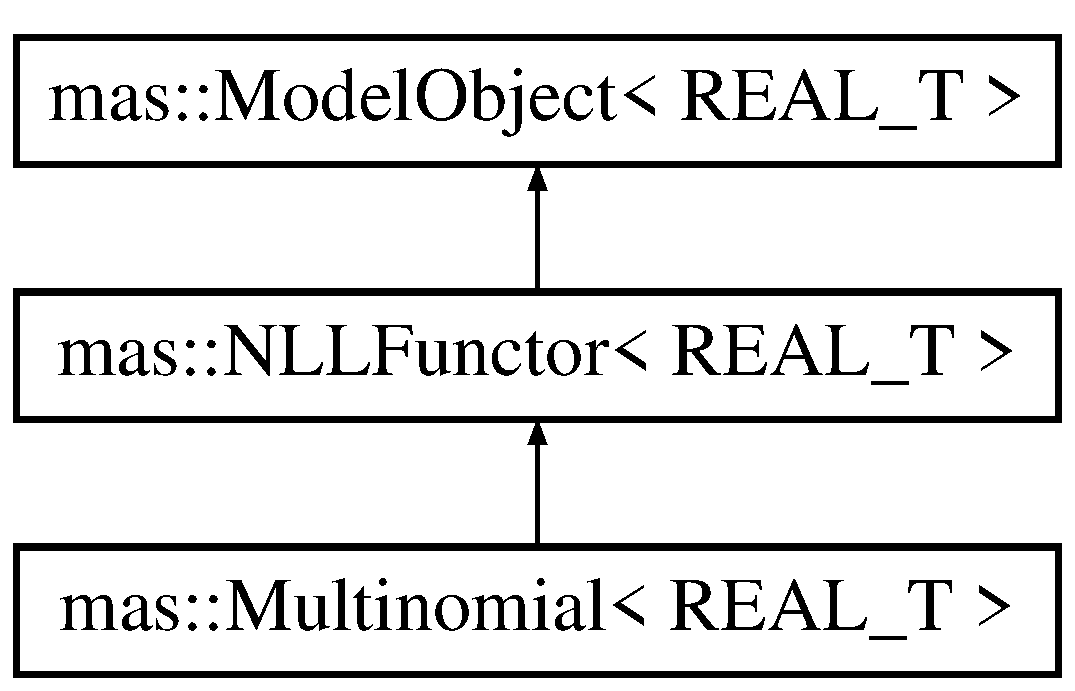
\includegraphics[height=3.000000cm]{structmas_1_1_multinomial}
\end{center}
\end{figure}
\subsection*{Public Types}
\begin{DoxyCompactItemize}
\item 
typedef \hyperlink{structmas_1_1_variable_trait}{Variable\-Trait}$<$ R\-E\-A\-L\-\_\-\-T $>$\\*
\-::\hyperlink{structmas_1_1_model_object_a4e62fdbb5826f8fac311262b888ab10a}{variable} \hyperlink{structmas_1_1_multinomial_a3d7e943ca6b28c275046a26559ce8efe}{variable}
\end{DoxyCompactItemize}
\subsection*{Public Member Functions}
\begin{DoxyCompactItemize}
\item 
\hyperlink{structmas_1_1_multinomial_ab96a958b976586557b7133911c3c2e01}{Multinomial} ()
\item 
\hyperlink{structmas_1_1_multinomial_ae285e7754e5db741e7c251e0f87d6b08}{Multinomial} (size\-\_\-t \hyperlink{structmas_1_1_n_l_l_functor_ac76e5d7e0808486b42ffdaea952dd19f}{years}, size\-\_\-t \hyperlink{structmas_1_1_n_l_l_functor_ac59c36239b1817b5bb357bf90dc4802d}{seasons}, size\-\_\-t \hyperlink{structmas_1_1_n_l_l_functor_aa70e461c812bff95770cda5dbb79b6b9}{ages})
\item 
virtual \hyperlink{structmas_1_1_model_object_a4e62fdbb5826f8fac311262b888ab10a}{variable} \hyperlink{structmas_1_1_multinomial_aaa2e60866cb5693bf048f09480547da4}{Evaluate} (const std\-::shared\-\_\-ptr$<$ \hyperlink{structmas_1_1_data_object}{Data\-Object}$<$ R\-E\-A\-L\-\_\-\-T $>$ $>$ \&observed, const std\-::vector$<$ \hyperlink{structmas_1_1_model_object_a4e62fdbb5826f8fac311262b888ab10a}{variable} $>$ \&predicted, size\-\_\-t N)
\item 
virtual std\-::string \hyperlink{structmas_1_1_multinomial_a90903904b06f2e5a79ffba4981fef34a}{To\-String} ()
\end{DoxyCompactItemize}
\subsection*{Additional Inherited Members}


\subsection{Detailed Description}
\subsubsection*{template$<$typename R\-E\-A\-L\-\_\-\-T$>$struct mas\-::\-Multinomial$<$ R\-E\-A\-L\-\_\-\-T $>$}



Definition at line 279 of file N\-L\-L\-Components.\-hpp.



\subsection{Member Typedef Documentation}
\hypertarget{structmas_1_1_multinomial_a3d7e943ca6b28c275046a26559ce8efe}{\index{mas\-::\-Multinomial@{mas\-::\-Multinomial}!variable@{variable}}
\index{variable@{variable}!mas::Multinomial@{mas\-::\-Multinomial}}
\subsubsection[{variable}]{\setlength{\rightskip}{0pt plus 5cm}template$<$typename R\-E\-A\-L\-\_\-\-T $>$ typedef {\bf Variable\-Trait}$<$R\-E\-A\-L\-\_\-\-T$>$\-::{\bf variable} {\bf mas\-::\-Multinomial}$<$ R\-E\-A\-L\-\_\-\-T $>$\-::{\bf variable}}}\label{structmas_1_1_multinomial_a3d7e943ca6b28c275046a26559ce8efe}


Definition at line 280 of file N\-L\-L\-Components.\-hpp.



\subsection{Constructor \& Destructor Documentation}
\hypertarget{structmas_1_1_multinomial_ab96a958b976586557b7133911c3c2e01}{\index{mas\-::\-Multinomial@{mas\-::\-Multinomial}!Multinomial@{Multinomial}}
\index{Multinomial@{Multinomial}!mas::Multinomial@{mas\-::\-Multinomial}}
\subsubsection[{Multinomial}]{\setlength{\rightskip}{0pt plus 5cm}template$<$typename R\-E\-A\-L\-\_\-\-T $>$ {\bf mas\-::\-Multinomial}$<$ R\-E\-A\-L\-\_\-\-T $>$\-::{\bf Multinomial} (
\begin{DoxyParamCaption}
{}
\end{DoxyParamCaption}
)\hspace{0.3cm}{\ttfamily [inline]}}}\label{structmas_1_1_multinomial_ab96a958b976586557b7133911c3c2e01}


Definition at line 282 of file N\-L\-L\-Components.\-hpp.

\hypertarget{structmas_1_1_multinomial_ae285e7754e5db741e7c251e0f87d6b08}{\index{mas\-::\-Multinomial@{mas\-::\-Multinomial}!Multinomial@{Multinomial}}
\index{Multinomial@{Multinomial}!mas::Multinomial@{mas\-::\-Multinomial}}
\subsubsection[{Multinomial}]{\setlength{\rightskip}{0pt plus 5cm}template$<$typename R\-E\-A\-L\-\_\-\-T $>$ {\bf mas\-::\-Multinomial}$<$ R\-E\-A\-L\-\_\-\-T $>$\-::{\bf Multinomial} (
\begin{DoxyParamCaption}
\item[{size\-\_\-t}]{years, }
\item[{size\-\_\-t}]{seasons, }
\item[{size\-\_\-t}]{ages}
\end{DoxyParamCaption}
)\hspace{0.3cm}{\ttfamily [inline]}}}\label{structmas_1_1_multinomial_ae285e7754e5db741e7c251e0f87d6b08}


Definition at line 285 of file N\-L\-L\-Components.\-hpp.



\subsection{Member Function Documentation}
\hypertarget{structmas_1_1_multinomial_aaa2e60866cb5693bf048f09480547da4}{\index{mas\-::\-Multinomial@{mas\-::\-Multinomial}!Evaluate@{Evaluate}}
\index{Evaluate@{Evaluate}!mas::Multinomial@{mas\-::\-Multinomial}}
\subsubsection[{Evaluate}]{\setlength{\rightskip}{0pt plus 5cm}template$<$typename R\-E\-A\-L\-\_\-\-T $>$ virtual {\bf variable} {\bf mas\-::\-Multinomial}$<$ R\-E\-A\-L\-\_\-\-T $>$\-::Evaluate (
\begin{DoxyParamCaption}
\item[{const std\-::shared\-\_\-ptr$<$ {\bf Data\-Object}$<$ R\-E\-A\-L\-\_\-\-T $>$ $>$ \&}]{observed, }
\item[{const std\-::vector$<$ {\bf variable} $>$ \&}]{predicted, }
\item[{size\-\_\-t}]{N}
\end{DoxyParamCaption}
)\hspace{0.3cm}{\ttfamily [inline]}, {\ttfamily [virtual]}}}\label{structmas_1_1_multinomial_aaa2e60866cb5693bf048f09480547da4}


Implements \hyperlink{structmas_1_1_n_l_l_functor_a463977400e35ad46ef60c334d452cd6c}{mas\-::\-N\-L\-L\-Functor$<$ R\-E\-A\-L\-\_\-\-T $>$}.



Definition at line 289 of file N\-L\-L\-Components.\-hpp.

\hypertarget{structmas_1_1_multinomial_a90903904b06f2e5a79ffba4981fef34a}{\index{mas\-::\-Multinomial@{mas\-::\-Multinomial}!To\-String@{To\-String}}
\index{To\-String@{To\-String}!mas::Multinomial@{mas\-::\-Multinomial}}
\subsubsection[{To\-String}]{\setlength{\rightskip}{0pt plus 5cm}template$<$typename R\-E\-A\-L\-\_\-\-T $>$ virtual std\-::string {\bf mas\-::\-Multinomial}$<$ R\-E\-A\-L\-\_\-\-T $>$\-::To\-String (
\begin{DoxyParamCaption}
{}
\end{DoxyParamCaption}
)\hspace{0.3cm}{\ttfamily [inline]}, {\ttfamily [virtual]}}}\label{structmas_1_1_multinomial_a90903904b06f2e5a79ffba4981fef34a}


Reimplemented from \hyperlink{structmas_1_1_n_l_l_functor_accd55442e1e88b423471b67c40860197}{mas\-::\-N\-L\-L\-Functor$<$ R\-E\-A\-L\-\_\-\-T $>$}.



Definition at line 321 of file N\-L\-L\-Components.\-hpp.



The documentation for this struct was generated from the following file\-:\begin{DoxyCompactItemize}
\item 
/home/oppy/\-Net\-Beans\-Projects/mas/\hyperlink{_n_l_l_components_8hpp}{N\-L\-L\-Components.\-hpp}\end{DoxyCompactItemize}

\hypertarget{structmas_1_1_multinomial_robust}{\section{mas\-:\-:Multinomial\-Robust$<$ R\-E\-A\-L\-\_\-\-T $>$ Struct Template Reference}
\label{structmas_1_1_multinomial_robust}\index{mas\-::\-Multinomial\-Robust$<$ R\-E\-A\-L\-\_\-\-T $>$@{mas\-::\-Multinomial\-Robust$<$ R\-E\-A\-L\-\_\-\-T $>$}}
}


{\ttfamily \#include $<$N\-L\-L\-Components.\-hpp$>$}

Inheritance diagram for mas\-:\-:Multinomial\-Robust$<$ R\-E\-A\-L\-\_\-\-T $>$\-:\begin{figure}[H]
\begin{center}
\leavevmode
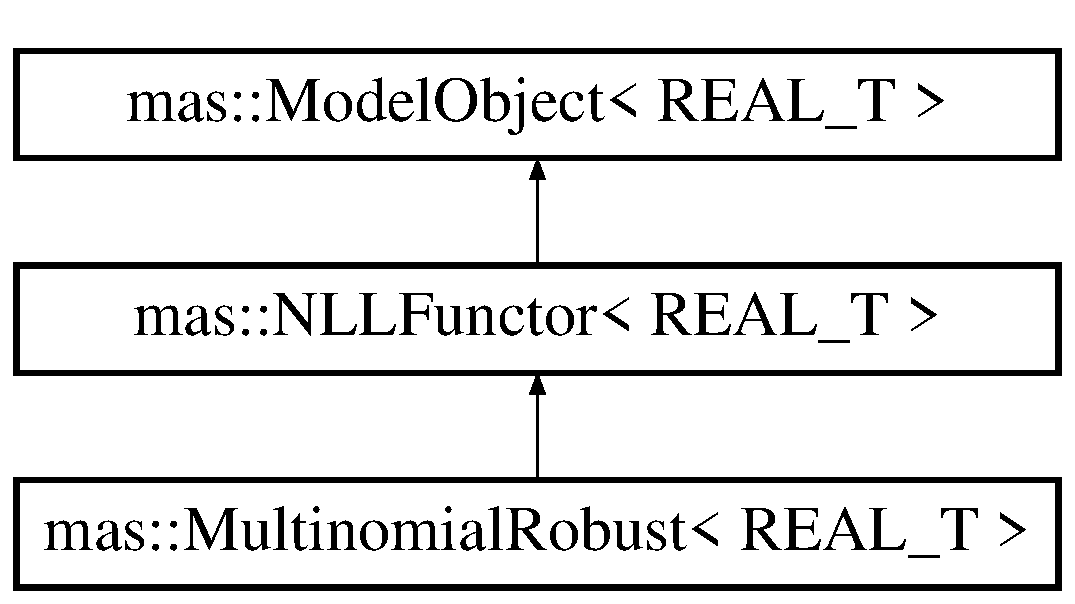
\includegraphics[height=3.000000cm]{structmas_1_1_multinomial_robust}
\end{center}
\end{figure}
\subsection*{Public Types}
\begin{DoxyCompactItemize}
\item 
typedef \hyperlink{structmas_1_1_variable_trait}{Variable\-Trait}$<$ R\-E\-A\-L\-\_\-\-T $>$\\*
\-::\hyperlink{structmas_1_1_model_object_a4e62fdbb5826f8fac311262b888ab10a}{variable} \hyperlink{structmas_1_1_multinomial_robust_a99b5fe82b4313d5a8d9b5d2ef7238259}{variable}
\end{DoxyCompactItemize}
\subsection*{Public Member Functions}
\begin{DoxyCompactItemize}
\item 
\hyperlink{structmas_1_1_multinomial_robust_a2e5610844b137bb244feb772c28329be}{Multinomial\-Robust} ()
\item 
\hyperlink{structmas_1_1_multinomial_robust_a446394824c179ca70723c1c5fb525f8e}{Multinomial\-Robust} (size\-\_\-t \hyperlink{structmas_1_1_n_l_l_functor_ac76e5d7e0808486b42ffdaea952dd19f}{years}, size\-\_\-t \hyperlink{structmas_1_1_n_l_l_functor_ac59c36239b1817b5bb357bf90dc4802d}{seasons}, size\-\_\-t \hyperlink{structmas_1_1_n_l_l_functor_aa70e461c812bff95770cda5dbb79b6b9}{ages})
\item 
virtual \hyperlink{structmas_1_1_model_object_a4e62fdbb5826f8fac311262b888ab10a}{variable} \hyperlink{structmas_1_1_multinomial_robust_a7c6e6e6fa0e96e92c3194a1c18b8745e}{Evaluate} (const std\-::shared\-\_\-ptr$<$ \hyperlink{structmas_1_1_data_object}{Data\-Object}$<$ R\-E\-A\-L\-\_\-\-T $>$ $>$ \&observed, const std\-::vector$<$ \hyperlink{structmas_1_1_model_object_a4e62fdbb5826f8fac311262b888ab10a}{variable} $>$ \&predicted, size\-\_\-t N)
\item 
virtual std\-::string \hyperlink{structmas_1_1_multinomial_robust_a57b1509abe3c1640fb0e24f636fbbd87}{To\-String} ()
\end{DoxyCompactItemize}
\subsection*{Public Attributes}
\begin{DoxyCompactItemize}
\item 
R\-E\-A\-L\-\_\-\-T \hyperlink{structmas_1_1_multinomial_robust_a7ef9fbeaf2f295d919b770a09b7f33b4}{epsilon} = static\-\_\-cast$<$R\-E\-A\-L\-\_\-\-T$>$ (1e-\/8)
\end{DoxyCompactItemize}


\subsection{Detailed Description}
\subsubsection*{template$<$typename R\-E\-A\-L\-\_\-\-T$>$struct mas\-::\-Multinomial\-Robust$<$ R\-E\-A\-L\-\_\-\-T $>$}



Definition at line 327 of file N\-L\-L\-Components.\-hpp.



\subsection{Member Typedef Documentation}
\hypertarget{structmas_1_1_multinomial_robust_a99b5fe82b4313d5a8d9b5d2ef7238259}{\index{mas\-::\-Multinomial\-Robust@{mas\-::\-Multinomial\-Robust}!variable@{variable}}
\index{variable@{variable}!mas::MultinomialRobust@{mas\-::\-Multinomial\-Robust}}
\subsubsection[{variable}]{\setlength{\rightskip}{0pt plus 5cm}template$<$typename R\-E\-A\-L\-\_\-\-T $>$ typedef {\bf Variable\-Trait}$<$R\-E\-A\-L\-\_\-\-T$>$\-::{\bf variable} {\bf mas\-::\-Multinomial\-Robust}$<$ R\-E\-A\-L\-\_\-\-T $>$\-::{\bf variable}}}\label{structmas_1_1_multinomial_robust_a99b5fe82b4313d5a8d9b5d2ef7238259}


Definition at line 328 of file N\-L\-L\-Components.\-hpp.



\subsection{Constructor \& Destructor Documentation}
\hypertarget{structmas_1_1_multinomial_robust_a2e5610844b137bb244feb772c28329be}{\index{mas\-::\-Multinomial\-Robust@{mas\-::\-Multinomial\-Robust}!Multinomial\-Robust@{Multinomial\-Robust}}
\index{Multinomial\-Robust@{Multinomial\-Robust}!mas::MultinomialRobust@{mas\-::\-Multinomial\-Robust}}
\subsubsection[{Multinomial\-Robust}]{\setlength{\rightskip}{0pt plus 5cm}template$<$typename R\-E\-A\-L\-\_\-\-T $>$ {\bf mas\-::\-Multinomial\-Robust}$<$ R\-E\-A\-L\-\_\-\-T $>$\-::{\bf Multinomial\-Robust} (
\begin{DoxyParamCaption}
{}
\end{DoxyParamCaption}
)\hspace{0.3cm}{\ttfamily [inline]}}}\label{structmas_1_1_multinomial_robust_a2e5610844b137bb244feb772c28329be}


Definition at line 331 of file N\-L\-L\-Components.\-hpp.

\hypertarget{structmas_1_1_multinomial_robust_a446394824c179ca70723c1c5fb525f8e}{\index{mas\-::\-Multinomial\-Robust@{mas\-::\-Multinomial\-Robust}!Multinomial\-Robust@{Multinomial\-Robust}}
\index{Multinomial\-Robust@{Multinomial\-Robust}!mas::MultinomialRobust@{mas\-::\-Multinomial\-Robust}}
\subsubsection[{Multinomial\-Robust}]{\setlength{\rightskip}{0pt plus 5cm}template$<$typename R\-E\-A\-L\-\_\-\-T $>$ {\bf mas\-::\-Multinomial\-Robust}$<$ R\-E\-A\-L\-\_\-\-T $>$\-::{\bf Multinomial\-Robust} (
\begin{DoxyParamCaption}
\item[{size\-\_\-t}]{years, }
\item[{size\-\_\-t}]{seasons, }
\item[{size\-\_\-t}]{ages}
\end{DoxyParamCaption}
)\hspace{0.3cm}{\ttfamily [inline]}}}\label{structmas_1_1_multinomial_robust_a446394824c179ca70723c1c5fb525f8e}


Definition at line 334 of file N\-L\-L\-Components.\-hpp.



\subsection{Member Function Documentation}
\hypertarget{structmas_1_1_multinomial_robust_a7c6e6e6fa0e96e92c3194a1c18b8745e}{\index{mas\-::\-Multinomial\-Robust@{mas\-::\-Multinomial\-Robust}!Evaluate@{Evaluate}}
\index{Evaluate@{Evaluate}!mas::MultinomialRobust@{mas\-::\-Multinomial\-Robust}}
\subsubsection[{Evaluate}]{\setlength{\rightskip}{0pt plus 5cm}template$<$typename R\-E\-A\-L\-\_\-\-T $>$ virtual {\bf variable} {\bf mas\-::\-Multinomial\-Robust}$<$ R\-E\-A\-L\-\_\-\-T $>$\-::Evaluate (
\begin{DoxyParamCaption}
\item[{const std\-::shared\-\_\-ptr$<$ {\bf Data\-Object}$<$ R\-E\-A\-L\-\_\-\-T $>$ $>$ \&}]{observed, }
\item[{const std\-::vector$<$ {\bf variable} $>$ \&}]{predicted, }
\item[{size\-\_\-t}]{N}
\end{DoxyParamCaption}
)\hspace{0.3cm}{\ttfamily [inline]}, {\ttfamily [virtual]}}}\label{structmas_1_1_multinomial_robust_a7c6e6e6fa0e96e92c3194a1c18b8745e}


Implements \hyperlink{structmas_1_1_n_l_l_functor_a463977400e35ad46ef60c334d452cd6c}{mas\-::\-N\-L\-L\-Functor$<$ R\-E\-A\-L\-\_\-\-T $>$}.



Definition at line 338 of file N\-L\-L\-Components.\-hpp.

\hypertarget{structmas_1_1_multinomial_robust_a57b1509abe3c1640fb0e24f636fbbd87}{\index{mas\-::\-Multinomial\-Robust@{mas\-::\-Multinomial\-Robust}!To\-String@{To\-String}}
\index{To\-String@{To\-String}!mas::MultinomialRobust@{mas\-::\-Multinomial\-Robust}}
\subsubsection[{To\-String}]{\setlength{\rightskip}{0pt plus 5cm}template$<$typename R\-E\-A\-L\-\_\-\-T $>$ virtual std\-::string {\bf mas\-::\-Multinomial\-Robust}$<$ R\-E\-A\-L\-\_\-\-T $>$\-::To\-String (
\begin{DoxyParamCaption}
{}
\end{DoxyParamCaption}
)\hspace{0.3cm}{\ttfamily [inline]}, {\ttfamily [virtual]}}}\label{structmas_1_1_multinomial_robust_a57b1509abe3c1640fb0e24f636fbbd87}


Reimplemented from \hyperlink{structmas_1_1_n_l_l_functor_accd55442e1e88b423471b67c40860197}{mas\-::\-N\-L\-L\-Functor$<$ R\-E\-A\-L\-\_\-\-T $>$}.



Definition at line 381 of file N\-L\-L\-Components.\-hpp.



\subsection{Member Data Documentation}
\hypertarget{structmas_1_1_multinomial_robust_a7ef9fbeaf2f295d919b770a09b7f33b4}{\index{mas\-::\-Multinomial\-Robust@{mas\-::\-Multinomial\-Robust}!epsilon@{epsilon}}
\index{epsilon@{epsilon}!mas::MultinomialRobust@{mas\-::\-Multinomial\-Robust}}
\subsubsection[{epsilon}]{\setlength{\rightskip}{0pt plus 5cm}template$<$typename R\-E\-A\-L\-\_\-\-T $>$ R\-E\-A\-L\-\_\-\-T {\bf mas\-::\-Multinomial\-Robust}$<$ R\-E\-A\-L\-\_\-\-T $>$\-::epsilon = static\-\_\-cast$<$R\-E\-A\-L\-\_\-\-T$>$ (1e-\/8)}}\label{structmas_1_1_multinomial_robust_a7ef9fbeaf2f295d919b770a09b7f33b4}


Definition at line 329 of file N\-L\-L\-Components.\-hpp.



The documentation for this struct was generated from the following file\-:\begin{DoxyCompactItemize}
\item 
/home/oppy/\-Net\-Beans\-Projects/mas/\hyperlink{_n_l_l_components_8hpp}{N\-L\-L\-Components.\-hpp}\end{DoxyCompactItemize}

\hypertarget{structmas_1_1_natural_mortality}{\section{mas\-:\-:Natural\-Mortality$<$ R\-E\-A\-L\-\_\-\-T $>$ Struct Template Reference}
\label{structmas_1_1_natural_mortality}\index{mas\-::\-Natural\-Mortality$<$ R\-E\-A\-L\-\_\-\-T $>$@{mas\-::\-Natural\-Mortality$<$ R\-E\-A\-L\-\_\-\-T $>$}}
}


{\ttfamily \#include $<$Mortality.\-hpp$>$}

Inheritance diagram for mas\-:\-:Natural\-Mortality$<$ R\-E\-A\-L\-\_\-\-T $>$\-:\begin{figure}[H]
\begin{center}
\leavevmode
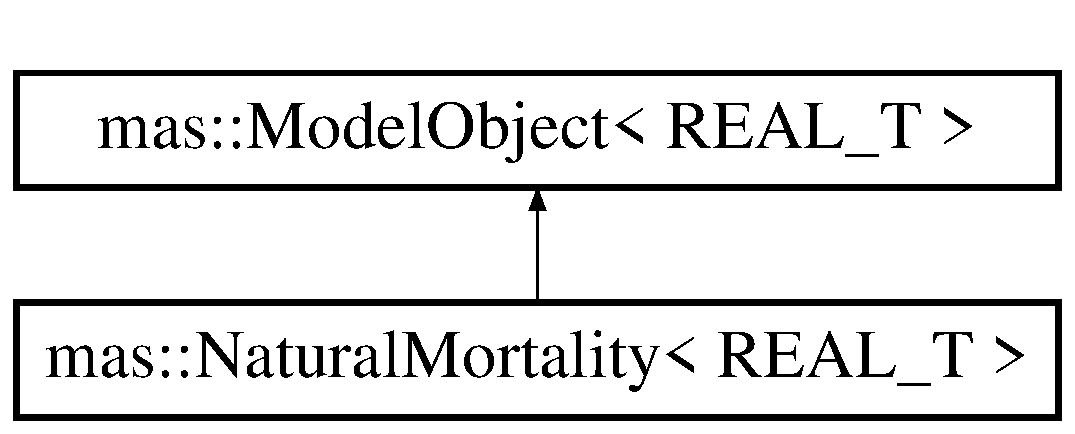
\includegraphics[height=2.000000cm]{structmas_1_1_natural_mortality}
\end{center}
\end{figure}
\subsection*{Public Types}
\begin{DoxyCompactItemize}
\item 
typedef \hyperlink{structmas_1_1_variable_trait}{Variable\-Trait}$<$ R\-E\-A\-L\-\_\-\-T $>$\\*
\-::\hyperlink{structmas_1_1_natural_mortality_a6f9549336ac14a2e7c2f587af6b066da}{variable} \hyperlink{structmas_1_1_natural_mortality_a6f9549336ac14a2e7c2f587af6b066da}{variable}
\item 
typedef std\-::unordered\-\_\-map\\*
$<$ R\-E\-A\-L\-\_\-\-T, \hyperlink{structmas_1_1_natural_mortality_a6f9549336ac14a2e7c2f587af6b066da}{variable} $>$\-::iterator \hyperlink{structmas_1_1_natural_mortality_a8c522fde4eb83dd74a0046d6b29cf807}{mortality\-\_\-iterator}
\end{DoxyCompactItemize}
\subsection*{Public Member Functions}
\begin{DoxyCompactItemize}
\item 
const \hyperlink{structmas_1_1_natural_mortality_a6f9549336ac14a2e7c2f587af6b066da}{variable} \hyperlink{structmas_1_1_natural_mortality_ad01169fda1c37d1bdbd162e39c7d676a}{Evaluate} (const int \&age\-\_\-index)
\item 
virtual const std\-::string \hyperlink{structmas_1_1_natural_mortality_ae788facfc8178ed04eeb1d31caada8f3}{To\-J\-S\-O\-N\-String} ()
\item 
virtual const std\-::string \hyperlink{structmas_1_1_natural_mortality_a9dbf045654a42cc4ecbb3c35e70afda7}{Name} ()
\end{DoxyCompactItemize}
\subsection*{Public Attributes}
\begin{DoxyCompactItemize}
\item 
std\-::vector$<$ \hyperlink{structmas_1_1_natural_mortality_a6f9549336ac14a2e7c2f587af6b066da}{variable} $>$ \hyperlink{structmas_1_1_natural_mortality_a3f161a8dcbf17c626f49d3e3bdb0afdf}{mortality\-\_\-vector}
\item 
std\-::unordered\-\_\-map$<$ R\-E\-A\-L\-\_\-\-T, \\*
\hyperlink{structmas_1_1_natural_mortality_a6f9549336ac14a2e7c2f587af6b066da}{variable} $>$ \hyperlink{structmas_1_1_natural_mortality_af324ad56891a3268c7ed06cd6fe5e1b0}{mortality}
\end{DoxyCompactItemize}


\subsection{Detailed Description}
\subsubsection*{template$<$typename R\-E\-A\-L\-\_\-\-T$>$struct mas\-::\-Natural\-Mortality$<$ R\-E\-A\-L\-\_\-\-T $>$}



Definition at line 42 of file Mortality.\-hpp.



\subsection{Member Typedef Documentation}
\hypertarget{structmas_1_1_natural_mortality_a8c522fde4eb83dd74a0046d6b29cf807}{\index{mas\-::\-Natural\-Mortality@{mas\-::\-Natural\-Mortality}!mortality\-\_\-iterator@{mortality\-\_\-iterator}}
\index{mortality\-\_\-iterator@{mortality\-\_\-iterator}!mas::NaturalMortality@{mas\-::\-Natural\-Mortality}}
\subsubsection[{mortality\-\_\-iterator}]{\setlength{\rightskip}{0pt plus 5cm}template$<$typename R\-E\-A\-L\-\_\-\-T $>$ typedef std\-::unordered\-\_\-map$<$R\-E\-A\-L\-\_\-\-T, {\bf variable}$>$\-::iterator {\bf mas\-::\-Natural\-Mortality}$<$ R\-E\-A\-L\-\_\-\-T $>$\-::{\bf mortality\-\_\-iterator}}}\label{structmas_1_1_natural_mortality_a8c522fde4eb83dd74a0046d6b29cf807}


Definition at line 48 of file Mortality.\-hpp.

\hypertarget{structmas_1_1_natural_mortality_a6f9549336ac14a2e7c2f587af6b066da}{\index{mas\-::\-Natural\-Mortality@{mas\-::\-Natural\-Mortality}!variable@{variable}}
\index{variable@{variable}!mas::NaturalMortality@{mas\-::\-Natural\-Mortality}}
\subsubsection[{variable}]{\setlength{\rightskip}{0pt plus 5cm}template$<$typename R\-E\-A\-L\-\_\-\-T $>$ typedef {\bf Variable\-Trait}$<$R\-E\-A\-L\-\_\-\-T$>$\-::{\bf variable} {\bf mas\-::\-Natural\-Mortality}$<$ R\-E\-A\-L\-\_\-\-T $>$\-::{\bf variable}}}\label{structmas_1_1_natural_mortality_a6f9549336ac14a2e7c2f587af6b066da}


Definition at line 43 of file Mortality.\-hpp.



\subsection{Member Function Documentation}
\hypertarget{structmas_1_1_natural_mortality_ad01169fda1c37d1bdbd162e39c7d676a}{\index{mas\-::\-Natural\-Mortality@{mas\-::\-Natural\-Mortality}!Evaluate@{Evaluate}}
\index{Evaluate@{Evaluate}!mas::NaturalMortality@{mas\-::\-Natural\-Mortality}}
\subsubsection[{Evaluate}]{\setlength{\rightskip}{0pt plus 5cm}template$<$typename R\-E\-A\-L\-\_\-\-T $>$ const {\bf variable} {\bf mas\-::\-Natural\-Mortality}$<$ R\-E\-A\-L\-\_\-\-T $>$\-::Evaluate (
\begin{DoxyParamCaption}
\item[{const int \&}]{age\-\_\-index}
\end{DoxyParamCaption}
)\hspace{0.3cm}{\ttfamily [inline]}}}\label{structmas_1_1_natural_mortality_ad01169fda1c37d1bdbd162e39c7d676a}


Definition at line 50 of file Mortality.\-hpp.

\hypertarget{structmas_1_1_natural_mortality_a9dbf045654a42cc4ecbb3c35e70afda7}{\index{mas\-::\-Natural\-Mortality@{mas\-::\-Natural\-Mortality}!Name@{Name}}
\index{Name@{Name}!mas::NaturalMortality@{mas\-::\-Natural\-Mortality}}
\subsubsection[{Name}]{\setlength{\rightskip}{0pt plus 5cm}template$<$typename R\-E\-A\-L\-\_\-\-T $>$ virtual const std\-::string {\bf mas\-::\-Natural\-Mortality}$<$ R\-E\-A\-L\-\_\-\-T $>$\-::Name (
\begin{DoxyParamCaption}
{}
\end{DoxyParamCaption}
)\hspace{0.3cm}{\ttfamily [inline]}, {\ttfamily [virtual]}}}\label{structmas_1_1_natural_mortality_a9dbf045654a42cc4ecbb3c35e70afda7}


Definition at line 96 of file Mortality.\-hpp.

\hypertarget{structmas_1_1_natural_mortality_ae788facfc8178ed04eeb1d31caada8f3}{\index{mas\-::\-Natural\-Mortality@{mas\-::\-Natural\-Mortality}!To\-J\-S\-O\-N\-String@{To\-J\-S\-O\-N\-String}}
\index{To\-J\-S\-O\-N\-String@{To\-J\-S\-O\-N\-String}!mas::NaturalMortality@{mas\-::\-Natural\-Mortality}}
\subsubsection[{To\-J\-S\-O\-N\-String}]{\setlength{\rightskip}{0pt plus 5cm}template$<$typename R\-E\-A\-L\-\_\-\-T $>$ virtual const std\-::string {\bf mas\-::\-Natural\-Mortality}$<$ R\-E\-A\-L\-\_\-\-T $>$\-::To\-J\-S\-O\-N\-String (
\begin{DoxyParamCaption}
{}
\end{DoxyParamCaption}
)\hspace{0.3cm}{\ttfamily [inline]}, {\ttfamily [virtual]}}}\label{structmas_1_1_natural_mortality_ae788facfc8178ed04eeb1d31caada8f3}


Reimplemented from \hyperlink{structmas_1_1_model_object_af40b3c89b11919fc5aea21dcf1cd027b}{mas\-::\-Model\-Object$<$ R\-E\-A\-L\-\_\-\-T $>$}.



Definition at line 55 of file Mortality.\-hpp.



\subsection{Member Data Documentation}
\hypertarget{structmas_1_1_natural_mortality_af324ad56891a3268c7ed06cd6fe5e1b0}{\index{mas\-::\-Natural\-Mortality@{mas\-::\-Natural\-Mortality}!mortality@{mortality}}
\index{mortality@{mortality}!mas::NaturalMortality@{mas\-::\-Natural\-Mortality}}
\subsubsection[{mortality}]{\setlength{\rightskip}{0pt plus 5cm}template$<$typename R\-E\-A\-L\-\_\-\-T $>$ std\-::unordered\-\_\-map$<$R\-E\-A\-L\-\_\-\-T, {\bf variable}$>$ {\bf mas\-::\-Natural\-Mortality}$<$ R\-E\-A\-L\-\_\-\-T $>$\-::mortality}}\label{structmas_1_1_natural_mortality_af324ad56891a3268c7ed06cd6fe5e1b0}


Definition at line 46 of file Mortality.\-hpp.

\hypertarget{structmas_1_1_natural_mortality_a3f161a8dcbf17c626f49d3e3bdb0afdf}{\index{mas\-::\-Natural\-Mortality@{mas\-::\-Natural\-Mortality}!mortality\-\_\-vector@{mortality\-\_\-vector}}
\index{mortality\-\_\-vector@{mortality\-\_\-vector}!mas::NaturalMortality@{mas\-::\-Natural\-Mortality}}
\subsubsection[{mortality\-\_\-vector}]{\setlength{\rightskip}{0pt plus 5cm}template$<$typename R\-E\-A\-L\-\_\-\-T $>$ std\-::vector$<${\bf variable}$>$ {\bf mas\-::\-Natural\-Mortality}$<$ R\-E\-A\-L\-\_\-\-T $>$\-::mortality\-\_\-vector}}\label{structmas_1_1_natural_mortality_a3f161a8dcbf17c626f49d3e3bdb0afdf}


Definition at line 44 of file Mortality.\-hpp.



The documentation for this struct was generated from the following file\-:\begin{DoxyCompactItemize}
\item 
/home/oppy/\-Net\-Beans\-Projects/mas/\hyperlink{_mortality_8hpp}{Mortality.\-hpp}\end{DoxyCompactItemize}

\hypertarget{classnetcdf__input}{\section{netcdf\-\_\-input Class Reference}
\label{classnetcdf__input}\index{netcdf\-\_\-input@{netcdf\-\_\-input}}
}


{\ttfamily \#include $<$Net\-C\-D\-F.\-hpp$>$}

\subsection*{Public Member Functions}
\begin{DoxyCompactItemize}
\item 
\hyperlink{classnetcdf__input_aed34aba0c7e7590dffb64417bb683ac8}{netcdf\-\_\-input} ()
\item 
\hyperlink{classnetcdf__input_acae75f119026d9ac5cc6814d0e94a908}{netcdf\-\_\-input} (const std\-::string \&path)
\item 
void \hyperlink{classnetcdf__input_a50314778372857039189a4f139448c68}{open} (const std\-::string \&path)
\item 
int \hyperlink{classnetcdf__input_a3d1d9f61be632b43137a249c3f4cc2e0}{read\-\_\-int} (const std\-::string \&variable, size\-\_\-t i, size\-\_\-t j=0, size\-\_\-t k=0, size\-\_\-t l=0, size\-\_\-t m=0, size\-\_\-t n=0)
\item 
long \hyperlink{classnetcdf__input_ad608df2a2400c2597fe20374d8555d11}{read\-\_\-long} (const std\-::string \&variable, size\-\_\-t i, size\-\_\-t j=0, size\-\_\-t k=0, size\-\_\-t l=0, size\-\_\-t m=0, size\-\_\-t n=0)
\item 
float \hyperlink{classnetcdf__input_a4e50818702ea85fe2bc2366b70383f22}{read\-\_\-float} (const std\-::string \&variable, size\-\_\-t i, size\-\_\-t j=0, size\-\_\-t k=0, size\-\_\-t l=0, size\-\_\-t m=0, size\-\_\-t n=0)
\item 
double \hyperlink{classnetcdf__input_a9b058e38c4a3cc0c8fa89597fbd8aaba}{read\-\_\-double} (const std\-::string \&variable, size\-\_\-t i, size\-\_\-t j=0, size\-\_\-t k=0, size\-\_\-t l=0, size\-\_\-t m=0, size\-\_\-t n=0)
\item 
std\-::multimap$<$ std\-::string, \\*
net\-C\-D\-F\-::\-Nc\-Var $>$ \hyperlink{classnetcdf__input_a6e474c0b56c8bc40c382b8c728a0d299}{get\-\_\-variables} ()
\item 
Nc\-Group\-Att \hyperlink{classnetcdf__input_a8174ba2c9f6f02574bbef5dd60703626}{get\-\_\-global\-\_\-attributes} (std\-::string att)
\item 
std\-::map$<$ std\-::string, Nc\-Var\-Att $>$ \hyperlink{classnetcdf__input_a0dcc20d4a2afd3b7b2be31514a549006}{get\-\_\-attributes} (std\-::string variable)
\item 
size\-\_\-t \hyperlink{classnetcdf__input_a02effe76acb8081382d78be1b0d60081}{dimension\-\_\-size} (const std\-::string \&name)
\end{DoxyCompactItemize}


\subsection{Detailed Description}


Definition at line 15 of file Net\-C\-D\-F.\-hpp.



\subsection{Constructor \& Destructor Documentation}
\hypertarget{classnetcdf__input_aed34aba0c7e7590dffb64417bb683ac8}{\index{netcdf\-\_\-input@{netcdf\-\_\-input}!netcdf\-\_\-input@{netcdf\-\_\-input}}
\index{netcdf\-\_\-input@{netcdf\-\_\-input}!netcdf_input@{netcdf\-\_\-input}}
\subsubsection[{netcdf\-\_\-input}]{\setlength{\rightskip}{0pt plus 5cm}netcdf\-\_\-input\-::netcdf\-\_\-input (
\begin{DoxyParamCaption}
{}
\end{DoxyParamCaption}
)\hspace{0.3cm}{\ttfamily [inline]}}}\label{classnetcdf__input_aed34aba0c7e7590dffb64417bb683ac8}


Definition at line 20 of file Net\-C\-D\-F.\-hpp.

\hypertarget{classnetcdf__input_acae75f119026d9ac5cc6814d0e94a908}{\index{netcdf\-\_\-input@{netcdf\-\_\-input}!netcdf\-\_\-input@{netcdf\-\_\-input}}
\index{netcdf\-\_\-input@{netcdf\-\_\-input}!netcdf_input@{netcdf\-\_\-input}}
\subsubsection[{netcdf\-\_\-input}]{\setlength{\rightskip}{0pt plus 5cm}netcdf\-\_\-input\-::netcdf\-\_\-input (
\begin{DoxyParamCaption}
\item[{const std\-::string \&}]{path}
\end{DoxyParamCaption}
)\hspace{0.3cm}{\ttfamily [inline]}}}\label{classnetcdf__input_acae75f119026d9ac5cc6814d0e94a908}


Definition at line 23 of file Net\-C\-D\-F.\-hpp.



\subsection{Member Function Documentation}
\hypertarget{classnetcdf__input_a02effe76acb8081382d78be1b0d60081}{\index{netcdf\-\_\-input@{netcdf\-\_\-input}!dimension\-\_\-size@{dimension\-\_\-size}}
\index{dimension\-\_\-size@{dimension\-\_\-size}!netcdf_input@{netcdf\-\_\-input}}
\subsubsection[{dimension\-\_\-size}]{\setlength{\rightskip}{0pt plus 5cm}size\-\_\-t netcdf\-\_\-input\-::dimension\-\_\-size (
\begin{DoxyParamCaption}
\item[{const std\-::string \&}]{name}
\end{DoxyParamCaption}
)\hspace{0.3cm}{\ttfamily [inline]}}}\label{classnetcdf__input_a02effe76acb8081382d78be1b0d60081}


Definition at line 174 of file Net\-C\-D\-F.\-hpp.

\hypertarget{classnetcdf__input_a0dcc20d4a2afd3b7b2be31514a549006}{\index{netcdf\-\_\-input@{netcdf\-\_\-input}!get\-\_\-attributes@{get\-\_\-attributes}}
\index{get\-\_\-attributes@{get\-\_\-attributes}!netcdf_input@{netcdf\-\_\-input}}
\subsubsection[{get\-\_\-attributes}]{\setlength{\rightskip}{0pt plus 5cm}std\-::map$<$std\-::string, Nc\-Var\-Att$>$ netcdf\-\_\-input\-::get\-\_\-attributes (
\begin{DoxyParamCaption}
\item[{std\-::string}]{variable}
\end{DoxyParamCaption}
)\hspace{0.3cm}{\ttfamily [inline]}}}\label{classnetcdf__input_a0dcc20d4a2afd3b7b2be31514a549006}


Definition at line 169 of file Net\-C\-D\-F.\-hpp.

\hypertarget{classnetcdf__input_a8174ba2c9f6f02574bbef5dd60703626}{\index{netcdf\-\_\-input@{netcdf\-\_\-input}!get\-\_\-global\-\_\-attributes@{get\-\_\-global\-\_\-attributes}}
\index{get\-\_\-global\-\_\-attributes@{get\-\_\-global\-\_\-attributes}!netcdf_input@{netcdf\-\_\-input}}
\subsubsection[{get\-\_\-global\-\_\-attributes}]{\setlength{\rightskip}{0pt plus 5cm}Nc\-Group\-Att netcdf\-\_\-input\-::get\-\_\-global\-\_\-attributes (
\begin{DoxyParamCaption}
\item[{std\-::string}]{att}
\end{DoxyParamCaption}
)\hspace{0.3cm}{\ttfamily [inline]}}}\label{classnetcdf__input_a8174ba2c9f6f02574bbef5dd60703626}


Definition at line 165 of file Net\-C\-D\-F.\-hpp.

\hypertarget{classnetcdf__input_a6e474c0b56c8bc40c382b8c728a0d299}{\index{netcdf\-\_\-input@{netcdf\-\_\-input}!get\-\_\-variables@{get\-\_\-variables}}
\index{get\-\_\-variables@{get\-\_\-variables}!netcdf_input@{netcdf\-\_\-input}}
\subsubsection[{get\-\_\-variables}]{\setlength{\rightskip}{0pt plus 5cm}std\-::multimap$<$std\-::string, net\-C\-D\-F\-::\-Nc\-Var$>$ netcdf\-\_\-input\-::get\-\_\-variables (
\begin{DoxyParamCaption}
{}
\end{DoxyParamCaption}
)\hspace{0.3cm}{\ttfamily [inline]}}}\label{classnetcdf__input_a6e474c0b56c8bc40c382b8c728a0d299}


Definition at line 161 of file Net\-C\-D\-F.\-hpp.

\hypertarget{classnetcdf__input_a50314778372857039189a4f139448c68}{\index{netcdf\-\_\-input@{netcdf\-\_\-input}!open@{open}}
\index{open@{open}!netcdf_input@{netcdf\-\_\-input}}
\subsubsection[{open}]{\setlength{\rightskip}{0pt plus 5cm}void netcdf\-\_\-input\-::open (
\begin{DoxyParamCaption}
\item[{const std\-::string \&}]{path}
\end{DoxyParamCaption}
)\hspace{0.3cm}{\ttfamily [inline]}}}\label{classnetcdf__input_a50314778372857039189a4f139448c68}


Definition at line 28 of file Net\-C\-D\-F.\-hpp.

\hypertarget{classnetcdf__input_a9b058e38c4a3cc0c8fa89597fbd8aaba}{\index{netcdf\-\_\-input@{netcdf\-\_\-input}!read\-\_\-double@{read\-\_\-double}}
\index{read\-\_\-double@{read\-\_\-double}!netcdf_input@{netcdf\-\_\-input}}
\subsubsection[{read\-\_\-double}]{\setlength{\rightskip}{0pt plus 5cm}double netcdf\-\_\-input\-::read\-\_\-double (
\begin{DoxyParamCaption}
\item[{const std\-::string \&}]{variable, }
\item[{size\-\_\-t}]{i, }
\item[{size\-\_\-t}]{j = {\ttfamily 0}, }
\item[{size\-\_\-t}]{k = {\ttfamily 0}, }
\item[{size\-\_\-t}]{l = {\ttfamily 0}, }
\item[{size\-\_\-t}]{m = {\ttfamily 0}, }
\item[{size\-\_\-t}]{n = {\ttfamily 0}}
\end{DoxyParamCaption}
)\hspace{0.3cm}{\ttfamily [inline]}}}\label{classnetcdf__input_a9b058e38c4a3cc0c8fa89597fbd8aaba}


Definition at line 129 of file Net\-C\-D\-F.\-hpp.

\hypertarget{classnetcdf__input_a4e50818702ea85fe2bc2366b70383f22}{\index{netcdf\-\_\-input@{netcdf\-\_\-input}!read\-\_\-float@{read\-\_\-float}}
\index{read\-\_\-float@{read\-\_\-float}!netcdf_input@{netcdf\-\_\-input}}
\subsubsection[{read\-\_\-float}]{\setlength{\rightskip}{0pt plus 5cm}float netcdf\-\_\-input\-::read\-\_\-float (
\begin{DoxyParamCaption}
\item[{const std\-::string \&}]{variable, }
\item[{size\-\_\-t}]{i, }
\item[{size\-\_\-t}]{j = {\ttfamily 0}, }
\item[{size\-\_\-t}]{k = {\ttfamily 0}, }
\item[{size\-\_\-t}]{l = {\ttfamily 0}, }
\item[{size\-\_\-t}]{m = {\ttfamily 0}, }
\item[{size\-\_\-t}]{n = {\ttfamily 0}}
\end{DoxyParamCaption}
)\hspace{0.3cm}{\ttfamily [inline]}}}\label{classnetcdf__input_a4e50818702ea85fe2bc2366b70383f22}


Definition at line 97 of file Net\-C\-D\-F.\-hpp.

\hypertarget{classnetcdf__input_a3d1d9f61be632b43137a249c3f4cc2e0}{\index{netcdf\-\_\-input@{netcdf\-\_\-input}!read\-\_\-int@{read\-\_\-int}}
\index{read\-\_\-int@{read\-\_\-int}!netcdf_input@{netcdf\-\_\-input}}
\subsubsection[{read\-\_\-int}]{\setlength{\rightskip}{0pt plus 5cm}int netcdf\-\_\-input\-::read\-\_\-int (
\begin{DoxyParamCaption}
\item[{const std\-::string \&}]{variable, }
\item[{size\-\_\-t}]{i, }
\item[{size\-\_\-t}]{j = {\ttfamily 0}, }
\item[{size\-\_\-t}]{k = {\ttfamily 0}, }
\item[{size\-\_\-t}]{l = {\ttfamily 0}, }
\item[{size\-\_\-t}]{m = {\ttfamily 0}, }
\item[{size\-\_\-t}]{n = {\ttfamily 0}}
\end{DoxyParamCaption}
)\hspace{0.3cm}{\ttfamily [inline]}}}\label{classnetcdf__input_a3d1d9f61be632b43137a249c3f4cc2e0}


Definition at line 33 of file Net\-C\-D\-F.\-hpp.

\hypertarget{classnetcdf__input_ad608df2a2400c2597fe20374d8555d11}{\index{netcdf\-\_\-input@{netcdf\-\_\-input}!read\-\_\-long@{read\-\_\-long}}
\index{read\-\_\-long@{read\-\_\-long}!netcdf_input@{netcdf\-\_\-input}}
\subsubsection[{read\-\_\-long}]{\setlength{\rightskip}{0pt plus 5cm}long netcdf\-\_\-input\-::read\-\_\-long (
\begin{DoxyParamCaption}
\item[{const std\-::string \&}]{variable, }
\item[{size\-\_\-t}]{i, }
\item[{size\-\_\-t}]{j = {\ttfamily 0}, }
\item[{size\-\_\-t}]{k = {\ttfamily 0}, }
\item[{size\-\_\-t}]{l = {\ttfamily 0}, }
\item[{size\-\_\-t}]{m = {\ttfamily 0}, }
\item[{size\-\_\-t}]{n = {\ttfamily 0}}
\end{DoxyParamCaption}
)\hspace{0.3cm}{\ttfamily [inline]}}}\label{classnetcdf__input_ad608df2a2400c2597fe20374d8555d11}


Definition at line 65 of file Net\-C\-D\-F.\-hpp.



The documentation for this class was generated from the following file\-:\begin{DoxyCompactItemize}
\item 
/home/oppy/\-Net\-Beans\-Projects/mas/\hyperlink{_net_c_d_f_8hpp}{Net\-C\-D\-F.\-hpp}\end{DoxyCompactItemize}

\hypertarget{classnetcdf__output}{\section{netcdf\-\_\-output Class Reference}
\label{classnetcdf__output}\index{netcdf\-\_\-output@{netcdf\-\_\-output}}
}


{\ttfamily \#include $<$Net\-C\-D\-F.\-hpp$>$}

\subsection*{Public Member Functions}
\begin{DoxyCompactItemize}
\item 
\hyperlink{classnetcdf__output_a607beec4937440be21f6a647b77385a0}{netcdf\-\_\-output} ()
\item 
\hyperlink{classnetcdf__output_af4474f9a65efa2795955412812a238fa}{netcdf\-\_\-output} (std\-::string path)
\item 
void \hyperlink{classnetcdf__output_a3216000bd093a7e80e784f93d625b9ef}{add\-\_\-variable} (const std\-::string \&name, const std\-::string \&data\-\_\-type, const std\-::vector$<$ std\-::string $>$ \&dimensions)
\item 
void \hyperlink{classnetcdf__output_abb18e538b6f4eb054efd58f76dd30bc1}{add\-\_\-dimension} (const std\-::string \&name, size\-\_\-t size)
\item 
size\-\_\-t \hyperlink{classnetcdf__output_a5323ef8e498baffcaade0e676cd7b794}{dimension\-\_\-size} (const std\-::string \&name)
\item 
void \hyperlink{classnetcdf__output_ad251a62975375a0be02db1a2b458d014}{add\-\_\-variable\-\_\-attribute} (const std\-::string \&variable\-\_\-name, const std\-::string \&attribute\-\_\-name, const std\-::string \&attribute)
\item 
void \hyperlink{classnetcdf__output_a6d23e007661a7e5704b77ade20bcd813}{add\-\_\-global\-\_\-attribute} (const std\-::string \&name, const std\-::string \&attribute)
\item 
void \hyperlink{classnetcdf__output_acd3ab83c891f21e15e84c4647ab53b63}{create} ()
\item 
void \hyperlink{classnetcdf__output_a76dbce9c73302b9671bc58bdc5c04241}{close} ()
\item 
void \hyperlink{classnetcdf__output_a083d5357edb0148e5279e178252b6fb0}{write\-\_\-int} (const std\-::string \&variable, const int \&value, size\-\_\-t i, size\-\_\-t j=0, size\-\_\-t k=0, size\-\_\-t l=0, size\-\_\-t m=0, size\-\_\-t n=0)
\item 
void \hyperlink{classnetcdf__output_aaa407a985dc11b104a01f71f45703d72}{write\-\_\-long} (const std\-::string \&variable, const long \&value, size\-\_\-t i, size\-\_\-t j=0, size\-\_\-t k=0, size\-\_\-t l=0, size\-\_\-t m=0, size\-\_\-t n=0)
\item 
void \hyperlink{classnetcdf__output_a10015d97fed8aadbb076cf875cd6795d}{write\-\_\-float} (const std\-::string \&variable, const float \&value, size\-\_\-t i, size\-\_\-t j=0, size\-\_\-t k=0, size\-\_\-t l=0, size\-\_\-t m=0, size\-\_\-t n=0)
\item 
void \hyperlink{classnetcdf__output_ac8834503fc85595aa4bd2689ca25c003}{write\-\_\-double} (const std\-::string \&variable, const double \&value, size\-\_\-t i, size\-\_\-t j=0, size\-\_\-t k=0, size\-\_\-t l=0, size\-\_\-t m=0, size\-\_\-t n=0)
\end{DoxyCompactItemize}
\subsection*{Public Attributes}
\begin{DoxyCompactItemize}
\item 
Nc\-File \hyperlink{classnetcdf__output_a4666c2e6af050a2bcc648f97cf063dbf}{output\-\_\-file}
\end{DoxyCompactItemize}


\subsection{Detailed Description}


Definition at line 181 of file Net\-C\-D\-F.\-hpp.



\subsection{Constructor \& Destructor Documentation}
\hypertarget{classnetcdf__output_a607beec4937440be21f6a647b77385a0}{\index{netcdf\-\_\-output@{netcdf\-\_\-output}!netcdf\-\_\-output@{netcdf\-\_\-output}}
\index{netcdf\-\_\-output@{netcdf\-\_\-output}!netcdf_output@{netcdf\-\_\-output}}
\subsubsection[{netcdf\-\_\-output}]{\setlength{\rightskip}{0pt plus 5cm}netcdf\-\_\-output\-::netcdf\-\_\-output (
\begin{DoxyParamCaption}
{}
\end{DoxyParamCaption}
)\hspace{0.3cm}{\ttfamily [inline]}}}\label{classnetcdf__output_a607beec4937440be21f6a647b77385a0}


Definition at line 187 of file Net\-C\-D\-F.\-hpp.

\hypertarget{classnetcdf__output_af4474f9a65efa2795955412812a238fa}{\index{netcdf\-\_\-output@{netcdf\-\_\-output}!netcdf\-\_\-output@{netcdf\-\_\-output}}
\index{netcdf\-\_\-output@{netcdf\-\_\-output}!netcdf_output@{netcdf\-\_\-output}}
\subsubsection[{netcdf\-\_\-output}]{\setlength{\rightskip}{0pt plus 5cm}netcdf\-\_\-output\-::netcdf\-\_\-output (
\begin{DoxyParamCaption}
\item[{std\-::string}]{path}
\end{DoxyParamCaption}
)\hspace{0.3cm}{\ttfamily [inline]}}}\label{classnetcdf__output_af4474f9a65efa2795955412812a238fa}


Definition at line 191 of file Net\-C\-D\-F.\-hpp.



\subsection{Member Function Documentation}
\hypertarget{classnetcdf__output_abb18e538b6f4eb054efd58f76dd30bc1}{\index{netcdf\-\_\-output@{netcdf\-\_\-output}!add\-\_\-dimension@{add\-\_\-dimension}}
\index{add\-\_\-dimension@{add\-\_\-dimension}!netcdf_output@{netcdf\-\_\-output}}
\subsubsection[{add\-\_\-dimension}]{\setlength{\rightskip}{0pt plus 5cm}void netcdf\-\_\-output\-::add\-\_\-dimension (
\begin{DoxyParamCaption}
\item[{const std\-::string \&}]{name, }
\item[{size\-\_\-t}]{size}
\end{DoxyParamCaption}
)\hspace{0.3cm}{\ttfamily [inline]}}}\label{classnetcdf__output_abb18e538b6f4eb054efd58f76dd30bc1}


Definition at line 216 of file Net\-C\-D\-F.\-hpp.

\hypertarget{classnetcdf__output_a6d23e007661a7e5704b77ade20bcd813}{\index{netcdf\-\_\-output@{netcdf\-\_\-output}!add\-\_\-global\-\_\-attribute@{add\-\_\-global\-\_\-attribute}}
\index{add\-\_\-global\-\_\-attribute@{add\-\_\-global\-\_\-attribute}!netcdf_output@{netcdf\-\_\-output}}
\subsubsection[{add\-\_\-global\-\_\-attribute}]{\setlength{\rightskip}{0pt plus 5cm}void netcdf\-\_\-output\-::add\-\_\-global\-\_\-attribute (
\begin{DoxyParamCaption}
\item[{const std\-::string \&}]{name, }
\item[{const std\-::string \&}]{attribute}
\end{DoxyParamCaption}
)\hspace{0.3cm}{\ttfamily [inline]}}}\label{classnetcdf__output_a6d23e007661a7e5704b77ade20bcd813}


Definition at line 230 of file Net\-C\-D\-F.\-hpp.

\hypertarget{classnetcdf__output_a3216000bd093a7e80e784f93d625b9ef}{\index{netcdf\-\_\-output@{netcdf\-\_\-output}!add\-\_\-variable@{add\-\_\-variable}}
\index{add\-\_\-variable@{add\-\_\-variable}!netcdf_output@{netcdf\-\_\-output}}
\subsubsection[{add\-\_\-variable}]{\setlength{\rightskip}{0pt plus 5cm}void netcdf\-\_\-output\-::add\-\_\-variable (
\begin{DoxyParamCaption}
\item[{const std\-::string \&}]{name, }
\item[{const std\-::string \&}]{data\-\_\-type, }
\item[{const std\-::vector$<$ std\-::string $>$ \&}]{dimensions}
\end{DoxyParamCaption}
)\hspace{0.3cm}{\ttfamily [inline]}}}\label{classnetcdf__output_a3216000bd093a7e80e784f93d625b9ef}


Definition at line 196 of file Net\-C\-D\-F.\-hpp.

\hypertarget{classnetcdf__output_ad251a62975375a0be02db1a2b458d014}{\index{netcdf\-\_\-output@{netcdf\-\_\-output}!add\-\_\-variable\-\_\-attribute@{add\-\_\-variable\-\_\-attribute}}
\index{add\-\_\-variable\-\_\-attribute@{add\-\_\-variable\-\_\-attribute}!netcdf_output@{netcdf\-\_\-output}}
\subsubsection[{add\-\_\-variable\-\_\-attribute}]{\setlength{\rightskip}{0pt plus 5cm}void netcdf\-\_\-output\-::add\-\_\-variable\-\_\-attribute (
\begin{DoxyParamCaption}
\item[{const std\-::string \&}]{variable\-\_\-name, }
\item[{const std\-::string \&}]{attribute\-\_\-name, }
\item[{const std\-::string \&}]{attribute}
\end{DoxyParamCaption}
)\hspace{0.3cm}{\ttfamily [inline]}}}\label{classnetcdf__output_ad251a62975375a0be02db1a2b458d014}


Definition at line 225 of file Net\-C\-D\-F.\-hpp.

\hypertarget{classnetcdf__output_a76dbce9c73302b9671bc58bdc5c04241}{\index{netcdf\-\_\-output@{netcdf\-\_\-output}!close@{close}}
\index{close@{close}!netcdf_output@{netcdf\-\_\-output}}
\subsubsection[{close}]{\setlength{\rightskip}{0pt plus 5cm}void netcdf\-\_\-output\-::close (
\begin{DoxyParamCaption}
{}
\end{DoxyParamCaption}
)\hspace{0.3cm}{\ttfamily [inline]}}}\label{classnetcdf__output_a76dbce9c73302b9671bc58bdc5c04241}


Definition at line 238 of file Net\-C\-D\-F.\-hpp.

\hypertarget{classnetcdf__output_acd3ab83c891f21e15e84c4647ab53b63}{\index{netcdf\-\_\-output@{netcdf\-\_\-output}!create@{create}}
\index{create@{create}!netcdf_output@{netcdf\-\_\-output}}
\subsubsection[{create}]{\setlength{\rightskip}{0pt plus 5cm}void netcdf\-\_\-output\-::create (
\begin{DoxyParamCaption}
{}
\end{DoxyParamCaption}
)\hspace{0.3cm}{\ttfamily [inline]}}}\label{classnetcdf__output_acd3ab83c891f21e15e84c4647ab53b63}


Definition at line 234 of file Net\-C\-D\-F.\-hpp.

\hypertarget{classnetcdf__output_a5323ef8e498baffcaade0e676cd7b794}{\index{netcdf\-\_\-output@{netcdf\-\_\-output}!dimension\-\_\-size@{dimension\-\_\-size}}
\index{dimension\-\_\-size@{dimension\-\_\-size}!netcdf_output@{netcdf\-\_\-output}}
\subsubsection[{dimension\-\_\-size}]{\setlength{\rightskip}{0pt plus 5cm}size\-\_\-t netcdf\-\_\-output\-::dimension\-\_\-size (
\begin{DoxyParamCaption}
\item[{const std\-::string \&}]{name}
\end{DoxyParamCaption}
)\hspace{0.3cm}{\ttfamily [inline]}}}\label{classnetcdf__output_a5323ef8e498baffcaade0e676cd7b794}


Definition at line 220 of file Net\-C\-D\-F.\-hpp.

\hypertarget{classnetcdf__output_ac8834503fc85595aa4bd2689ca25c003}{\index{netcdf\-\_\-output@{netcdf\-\_\-output}!write\-\_\-double@{write\-\_\-double}}
\index{write\-\_\-double@{write\-\_\-double}!netcdf_output@{netcdf\-\_\-output}}
\subsubsection[{write\-\_\-double}]{\setlength{\rightskip}{0pt plus 5cm}void netcdf\-\_\-output\-::write\-\_\-double (
\begin{DoxyParamCaption}
\item[{const std\-::string \&}]{variable, }
\item[{const double \&}]{value, }
\item[{size\-\_\-t}]{i, }
\item[{size\-\_\-t}]{j = {\ttfamily 0}, }
\item[{size\-\_\-t}]{k = {\ttfamily 0}, }
\item[{size\-\_\-t}]{l = {\ttfamily 0}, }
\item[{size\-\_\-t}]{m = {\ttfamily 0}, }
\item[{size\-\_\-t}]{n = {\ttfamily 0}}
\end{DoxyParamCaption}
)\hspace{0.3cm}{\ttfamily [inline]}}}\label{classnetcdf__output_ac8834503fc85595aa4bd2689ca25c003}


Definition at line 335 of file Net\-C\-D\-F.\-hpp.

\hypertarget{classnetcdf__output_a10015d97fed8aadbb076cf875cd6795d}{\index{netcdf\-\_\-output@{netcdf\-\_\-output}!write\-\_\-float@{write\-\_\-float}}
\index{write\-\_\-float@{write\-\_\-float}!netcdf_output@{netcdf\-\_\-output}}
\subsubsection[{write\-\_\-float}]{\setlength{\rightskip}{0pt plus 5cm}void netcdf\-\_\-output\-::write\-\_\-float (
\begin{DoxyParamCaption}
\item[{const std\-::string \&}]{variable, }
\item[{const float \&}]{value, }
\item[{size\-\_\-t}]{i, }
\item[{size\-\_\-t}]{j = {\ttfamily 0}, }
\item[{size\-\_\-t}]{k = {\ttfamily 0}, }
\item[{size\-\_\-t}]{l = {\ttfamily 0}, }
\item[{size\-\_\-t}]{m = {\ttfamily 0}, }
\item[{size\-\_\-t}]{n = {\ttfamily 0}}
\end{DoxyParamCaption}
)\hspace{0.3cm}{\ttfamily [inline]}}}\label{classnetcdf__output_a10015d97fed8aadbb076cf875cd6795d}


Definition at line 304 of file Net\-C\-D\-F.\-hpp.

\hypertarget{classnetcdf__output_a083d5357edb0148e5279e178252b6fb0}{\index{netcdf\-\_\-output@{netcdf\-\_\-output}!write\-\_\-int@{write\-\_\-int}}
\index{write\-\_\-int@{write\-\_\-int}!netcdf_output@{netcdf\-\_\-output}}
\subsubsection[{write\-\_\-int}]{\setlength{\rightskip}{0pt plus 5cm}void netcdf\-\_\-output\-::write\-\_\-int (
\begin{DoxyParamCaption}
\item[{const std\-::string \&}]{variable, }
\item[{const int \&}]{value, }
\item[{size\-\_\-t}]{i, }
\item[{size\-\_\-t}]{j = {\ttfamily 0}, }
\item[{size\-\_\-t}]{k = {\ttfamily 0}, }
\item[{size\-\_\-t}]{l = {\ttfamily 0}, }
\item[{size\-\_\-t}]{m = {\ttfamily 0}, }
\item[{size\-\_\-t}]{n = {\ttfamily 0}}
\end{DoxyParamCaption}
)\hspace{0.3cm}{\ttfamily [inline]}}}\label{classnetcdf__output_a083d5357edb0148e5279e178252b6fb0}


Definition at line 242 of file Net\-C\-D\-F.\-hpp.

\hypertarget{classnetcdf__output_aaa407a985dc11b104a01f71f45703d72}{\index{netcdf\-\_\-output@{netcdf\-\_\-output}!write\-\_\-long@{write\-\_\-long}}
\index{write\-\_\-long@{write\-\_\-long}!netcdf_output@{netcdf\-\_\-output}}
\subsubsection[{write\-\_\-long}]{\setlength{\rightskip}{0pt plus 5cm}void netcdf\-\_\-output\-::write\-\_\-long (
\begin{DoxyParamCaption}
\item[{const std\-::string \&}]{variable, }
\item[{const long \&}]{value, }
\item[{size\-\_\-t}]{i, }
\item[{size\-\_\-t}]{j = {\ttfamily 0}, }
\item[{size\-\_\-t}]{k = {\ttfamily 0}, }
\item[{size\-\_\-t}]{l = {\ttfamily 0}, }
\item[{size\-\_\-t}]{m = {\ttfamily 0}, }
\item[{size\-\_\-t}]{n = {\ttfamily 0}}
\end{DoxyParamCaption}
)\hspace{0.3cm}{\ttfamily [inline]}}}\label{classnetcdf__output_aaa407a985dc11b104a01f71f45703d72}


Definition at line 273 of file Net\-C\-D\-F.\-hpp.



\subsection{Member Data Documentation}
\hypertarget{classnetcdf__output_a4666c2e6af050a2bcc648f97cf063dbf}{\index{netcdf\-\_\-output@{netcdf\-\_\-output}!output\-\_\-file@{output\-\_\-file}}
\index{output\-\_\-file@{output\-\_\-file}!netcdf_output@{netcdf\-\_\-output}}
\subsubsection[{output\-\_\-file}]{\setlength{\rightskip}{0pt plus 5cm}Nc\-File netcdf\-\_\-output\-::output\-\_\-file}}\label{classnetcdf__output_a4666c2e6af050a2bcc648f97cf063dbf}


Definition at line 185 of file Net\-C\-D\-F.\-hpp.



The documentation for this class was generated from the following file\-:\begin{DoxyCompactItemize}
\item 
/home/oppy/\-Net\-Beans\-Projects/mas/\hyperlink{_net_c_d_f_8hpp}{Net\-C\-D\-F.\-hpp}\end{DoxyCompactItemize}

\hypertarget{structmas_1_1_n_l_l_component}{\section{mas\-:\-:N\-L\-L\-Component$<$ R\-E\-A\-L\-\_\-\-T $>$ Struct Template Reference}
\label{structmas_1_1_n_l_l_component}\index{mas\-::\-N\-L\-L\-Component$<$ R\-E\-A\-L\-\_\-\-T $>$@{mas\-::\-N\-L\-L\-Component$<$ R\-E\-A\-L\-\_\-\-T $>$}}
}


{\ttfamily \#include $<$N\-L\-L\-Components.\-hpp$>$}

\subsection*{Public Types}
\begin{DoxyCompactItemize}
\item 
typedef \hyperlink{structmas_1_1_variable_trait}{Variable\-Trait}$<$ R\-E\-A\-L\-\_\-\-T $>$\\*
\-::\hyperlink{structmas_1_1_n_l_l_component_a867afdda641b99341b7ebcbaea001f94}{variable} \hyperlink{structmas_1_1_n_l_l_component_a867afdda641b99341b7ebcbaea001f94}{variable}
\end{DoxyCompactItemize}
\subsection*{Public Member Functions}
\begin{DoxyCompactItemize}
\item 
\hyperlink{structmas_1_1_n_l_l_component_a0722b21b60ba301e910d34106fac2534}{N\-L\-L\-Component} (std\-::vector$<$ \hyperlink{structmas_1_1_n_l_l_component_a867afdda641b99341b7ebcbaea001f94}{variable} $>$ $\ast$\hyperlink{structmas_1_1_n_l_l_component_a1d5439e34e306b6d3cfabfa7511f4885}{estimated}, std\-::shared\-\_\-ptr$<$ \hyperlink{structmas_1_1_data_object}{Data\-Object}$<$ R\-E\-A\-L\-\_\-\-T $>$ $>$ \hyperlink{structmas_1_1_n_l_l_component_a82a2b4e08e4b1f9509aae06b0622bcef}{observed}, std\-::shared\-\_\-ptr$<$ \hyperlink{structmas_1_1_n_l_l_functor}{mas\-::\-N\-L\-L\-Functor}$<$ R\-E\-A\-L\-\_\-\-T $>$ $>$ \hyperlink{structmas_1_1_n_l_l_component_aac558bbcbc7a6d23b86b59bde0b2feed}{nll\-\_\-functor})
\item 
void \hyperlink{structmas_1_1_n_l_l_component_ac8865fe2326ebc453fc69d7c7d0852a5}{Evaluate} (\hyperlink{structmas_1_1_n_l_l_component_a867afdda641b99341b7ebcbaea001f94}{variable} \&nll\-\_\-c)
\end{DoxyCompactItemize}
\subsection*{Public Attributes}
\begin{DoxyCompactItemize}
\item 
std\-::vector$<$ \hyperlink{structmas_1_1_n_l_l_component_a867afdda641b99341b7ebcbaea001f94}{variable} $>$ $\ast$ \hyperlink{structmas_1_1_n_l_l_component_a1d5439e34e306b6d3cfabfa7511f4885}{estimated}
\item 
std\-::shared\-\_\-ptr$<$ \hyperlink{structmas_1_1_data_object}{Data\-Object}\\*
$<$ R\-E\-A\-L\-\_\-\-T $>$ $>$ \hyperlink{structmas_1_1_n_l_l_component_a82a2b4e08e4b1f9509aae06b0622bcef}{observed}
\item 
std\-::shared\-\_\-ptr\\*
$<$ \hyperlink{structmas_1_1_n_l_l_functor}{mas\-::\-N\-L\-L\-Functor}$<$ R\-E\-A\-L\-\_\-\-T $>$ $>$ \hyperlink{structmas_1_1_n_l_l_component_aac558bbcbc7a6d23b86b59bde0b2feed}{nll\-\_\-functor}
\item 
size\-\_\-t \hyperlink{structmas_1_1_n_l_l_component_ae00089e4495dceff480b3e5d757a28c8}{N}
\end{DoxyCompactItemize}


\subsection{Detailed Description}
\subsubsection*{template$<$typename R\-E\-A\-L\-\_\-\-T$>$struct mas\-::\-N\-L\-L\-Component$<$ R\-E\-A\-L\-\_\-\-T $>$}



Definition at line 387 of file N\-L\-L\-Components.\-hpp.



\subsection{Member Typedef Documentation}
\hypertarget{structmas_1_1_n_l_l_component_a867afdda641b99341b7ebcbaea001f94}{\index{mas\-::\-N\-L\-L\-Component@{mas\-::\-N\-L\-L\-Component}!variable@{variable}}
\index{variable@{variable}!mas::NLLComponent@{mas\-::\-N\-L\-L\-Component}}
\subsubsection[{variable}]{\setlength{\rightskip}{0pt plus 5cm}template$<$typename R\-E\-A\-L\-\_\-\-T $>$ typedef {\bf Variable\-Trait}$<$R\-E\-A\-L\-\_\-\-T$>$\-::{\bf variable} {\bf mas\-::\-N\-L\-L\-Component}$<$ R\-E\-A\-L\-\_\-\-T $>$\-::{\bf variable}}}\label{structmas_1_1_n_l_l_component_a867afdda641b99341b7ebcbaea001f94}


Definition at line 388 of file N\-L\-L\-Components.\-hpp.



\subsection{Constructor \& Destructor Documentation}
\hypertarget{structmas_1_1_n_l_l_component_a0722b21b60ba301e910d34106fac2534}{\index{mas\-::\-N\-L\-L\-Component@{mas\-::\-N\-L\-L\-Component}!N\-L\-L\-Component@{N\-L\-L\-Component}}
\index{N\-L\-L\-Component@{N\-L\-L\-Component}!mas::NLLComponent@{mas\-::\-N\-L\-L\-Component}}
\subsubsection[{N\-L\-L\-Component}]{\setlength{\rightskip}{0pt plus 5cm}template$<$typename R\-E\-A\-L\-\_\-\-T $>$ {\bf mas\-::\-N\-L\-L\-Component}$<$ R\-E\-A\-L\-\_\-\-T $>$\-::{\bf N\-L\-L\-Component} (
\begin{DoxyParamCaption}
\item[{std\-::vector$<$ {\bf variable} $>$ $\ast$}]{estimated, }
\item[{std\-::shared\-\_\-ptr$<$ {\bf Data\-Object}$<$ R\-E\-A\-L\-\_\-\-T $>$ $>$}]{observed, }
\item[{std\-::shared\-\_\-ptr$<$ {\bf mas\-::\-N\-L\-L\-Functor}$<$ R\-E\-A\-L\-\_\-\-T $>$ $>$}]{nll\-\_\-functor}
\end{DoxyParamCaption}
)\hspace{0.3cm}{\ttfamily [inline]}}}\label{structmas_1_1_n_l_l_component_a0722b21b60ba301e910d34106fac2534}


Definition at line 394 of file N\-L\-L\-Components.\-hpp.



\subsection{Member Function Documentation}
\hypertarget{structmas_1_1_n_l_l_component_ac8865fe2326ebc453fc69d7c7d0852a5}{\index{mas\-::\-N\-L\-L\-Component@{mas\-::\-N\-L\-L\-Component}!Evaluate@{Evaluate}}
\index{Evaluate@{Evaluate}!mas::NLLComponent@{mas\-::\-N\-L\-L\-Component}}
\subsubsection[{Evaluate}]{\setlength{\rightskip}{0pt plus 5cm}template$<$typename R\-E\-A\-L\-\_\-\-T $>$ void {\bf mas\-::\-N\-L\-L\-Component}$<$ R\-E\-A\-L\-\_\-\-T $>$\-::Evaluate (
\begin{DoxyParamCaption}
\item[{{\bf variable} \&}]{nll\-\_\-c}
\end{DoxyParamCaption}
)\hspace{0.3cm}{\ttfamily [inline]}}}\label{structmas_1_1_n_l_l_component_ac8865fe2326ebc453fc69d7c7d0852a5}


Definition at line 413 of file N\-L\-L\-Components.\-hpp.



\subsection{Member Data Documentation}
\hypertarget{structmas_1_1_n_l_l_component_a1d5439e34e306b6d3cfabfa7511f4885}{\index{mas\-::\-N\-L\-L\-Component@{mas\-::\-N\-L\-L\-Component}!estimated@{estimated}}
\index{estimated@{estimated}!mas::NLLComponent@{mas\-::\-N\-L\-L\-Component}}
\subsubsection[{estimated}]{\setlength{\rightskip}{0pt plus 5cm}template$<$typename R\-E\-A\-L\-\_\-\-T $>$ std\-::vector$<${\bf variable}$>$$\ast$ {\bf mas\-::\-N\-L\-L\-Component}$<$ R\-E\-A\-L\-\_\-\-T $>$\-::estimated}}\label{structmas_1_1_n_l_l_component_a1d5439e34e306b6d3cfabfa7511f4885}


Definition at line 389 of file N\-L\-L\-Components.\-hpp.

\hypertarget{structmas_1_1_n_l_l_component_ae00089e4495dceff480b3e5d757a28c8}{\index{mas\-::\-N\-L\-L\-Component@{mas\-::\-N\-L\-L\-Component}!N@{N}}
\index{N@{N}!mas::NLLComponent@{mas\-::\-N\-L\-L\-Component}}
\subsubsection[{N}]{\setlength{\rightskip}{0pt plus 5cm}template$<$typename R\-E\-A\-L\-\_\-\-T $>$ size\-\_\-t {\bf mas\-::\-N\-L\-L\-Component}$<$ R\-E\-A\-L\-\_\-\-T $>$\-::N}}\label{structmas_1_1_n_l_l_component_ae00089e4495dceff480b3e5d757a28c8}


Definition at line 392 of file N\-L\-L\-Components.\-hpp.

\hypertarget{structmas_1_1_n_l_l_component_aac558bbcbc7a6d23b86b59bde0b2feed}{\index{mas\-::\-N\-L\-L\-Component@{mas\-::\-N\-L\-L\-Component}!nll\-\_\-functor@{nll\-\_\-functor}}
\index{nll\-\_\-functor@{nll\-\_\-functor}!mas::NLLComponent@{mas\-::\-N\-L\-L\-Component}}
\subsubsection[{nll\-\_\-functor}]{\setlength{\rightskip}{0pt plus 5cm}template$<$typename R\-E\-A\-L\-\_\-\-T $>$ std\-::shared\-\_\-ptr$<${\bf mas\-::\-N\-L\-L\-Functor}$<$R\-E\-A\-L\-\_\-\-T$>$ $>$ {\bf mas\-::\-N\-L\-L\-Component}$<$ R\-E\-A\-L\-\_\-\-T $>$\-::nll\-\_\-functor}}\label{structmas_1_1_n_l_l_component_aac558bbcbc7a6d23b86b59bde0b2feed}


Definition at line 391 of file N\-L\-L\-Components.\-hpp.

\hypertarget{structmas_1_1_n_l_l_component_a82a2b4e08e4b1f9509aae06b0622bcef}{\index{mas\-::\-N\-L\-L\-Component@{mas\-::\-N\-L\-L\-Component}!observed@{observed}}
\index{observed@{observed}!mas::NLLComponent@{mas\-::\-N\-L\-L\-Component}}
\subsubsection[{observed}]{\setlength{\rightskip}{0pt plus 5cm}template$<$typename R\-E\-A\-L\-\_\-\-T $>$ std\-::shared\-\_\-ptr$<${\bf Data\-Object}$<$R\-E\-A\-L\-\_\-\-T$>$ $>$ {\bf mas\-::\-N\-L\-L\-Component}$<$ R\-E\-A\-L\-\_\-\-T $>$\-::observed}}\label{structmas_1_1_n_l_l_component_a82a2b4e08e4b1f9509aae06b0622bcef}


Definition at line 390 of file N\-L\-L\-Components.\-hpp.



The documentation for this struct was generated from the following file\-:\begin{DoxyCompactItemize}
\item 
/home/oppy/\-Net\-Beans\-Projects/mas/\hyperlink{_n_l_l_components_8hpp}{N\-L\-L\-Components.\-hpp}\end{DoxyCompactItemize}

\hypertarget{structmas_1_1_n_l_l_functor}{\section{mas\-:\-:N\-L\-L\-Functor$<$ R\-E\-A\-L\-\_\-\-T $>$ Struct Template Reference}
\label{structmas_1_1_n_l_l_functor}\index{mas\-::\-N\-L\-L\-Functor$<$ R\-E\-A\-L\-\_\-\-T $>$@{mas\-::\-N\-L\-L\-Functor$<$ R\-E\-A\-L\-\_\-\-T $>$}}
}


{\ttfamily \#include $<$N\-L\-L\-Components.\-hpp$>$}

Inheritance diagram for mas\-:\-:N\-L\-L\-Functor$<$ R\-E\-A\-L\-\_\-\-T $>$\-:\begin{figure}[H]
\begin{center}
\leavevmode
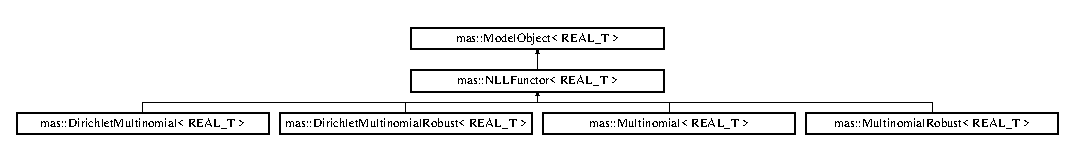
\includegraphics[height=1.578947cm]{structmas_1_1_n_l_l_functor}
\end{center}
\end{figure}
\subsection*{Public Types}
\begin{DoxyCompactItemize}
\item 
typedef \hyperlink{structmas_1_1_variable_trait}{Variable\-Trait}$<$ R\-E\-A\-L\-\_\-\-T $>$\\*
\-::\hyperlink{structmas_1_1_model_object_a4e62fdbb5826f8fac311262b888ab10a}{variable} \hyperlink{structmas_1_1_n_l_l_functor_af0af5a53b4f1a30a9cf498e6d284c402}{variable}
\end{DoxyCompactItemize}
\subsection*{Public Member Functions}
\begin{DoxyCompactItemize}
\item 
\hyperlink{structmas_1_1_n_l_l_functor_aeab80f44a0ac094884e439c18ae6b685}{N\-L\-L\-Functor} ()
\item 
\hyperlink{structmas_1_1_n_l_l_functor_a47364fea079a116df7f7ad860f977c5a}{N\-L\-L\-Functor} (size\-\_\-t \hyperlink{structmas_1_1_n_l_l_functor_ac76e5d7e0808486b42ffdaea952dd19f}{years}, size\-\_\-t \hyperlink{structmas_1_1_n_l_l_functor_ac59c36239b1817b5bb357bf90dc4802d}{seasons}, size\-\_\-t \hyperlink{structmas_1_1_n_l_l_functor_aa70e461c812bff95770cda5dbb79b6b9}{ages})
\item 
virtual \hyperlink{structmas_1_1_model_object_a4e62fdbb5826f8fac311262b888ab10a}{variable} \hyperlink{structmas_1_1_n_l_l_functor_a463977400e35ad46ef60c334d452cd6c}{Evaluate} (const std\-::shared\-\_\-ptr$<$ \hyperlink{structmas_1_1_data_object}{Data\-Object}$<$ R\-E\-A\-L\-\_\-\-T $>$ $>$ \&observed, const std\-::vector$<$ \hyperlink{structmas_1_1_model_object_a4e62fdbb5826f8fac311262b888ab10a}{variable} $>$ \&predicted, size\-\_\-t N)=0
\item 
virtual const R\-E\-A\-L\-\_\-\-T \hyperlink{structmas_1_1_n_l_l_functor_af86f7157edbcace46138c9b8cb03ddf0}{Neff} ()
\item 
virtual std\-::string \hyperlink{structmas_1_1_n_l_l_functor_accd55442e1e88b423471b67c40860197}{To\-String} ()
\end{DoxyCompactItemize}
\subsection*{Public Attributes}
\begin{DoxyCompactItemize}
\item 
size\-\_\-t \hyperlink{structmas_1_1_n_l_l_functor_ac76e5d7e0808486b42ffdaea952dd19f}{years}
\item 
size\-\_\-t \hyperlink{structmas_1_1_n_l_l_functor_ac59c36239b1817b5bb357bf90dc4802d}{seasons}
\item 
size\-\_\-t \hyperlink{structmas_1_1_n_l_l_functor_aa70e461c812bff95770cda5dbb79b6b9}{ages}
\item 
R\-E\-A\-L\-\_\-\-T \hyperlink{structmas_1_1_n_l_l_functor_ac7fe7be14787477c775c1c628a454118}{neff}
\item 
std\-::shared\-\_\-ptr\\*
$<$ \hyperlink{structmas_1_1_data_object}{mas\-::\-Data\-Object}$<$ R\-E\-A\-L\-\_\-\-T $>$ $>$ \hyperlink{structmas_1_1_n_l_l_functor_a50032d1f03b5743690723c33b62d2b4d}{lambda}
\end{DoxyCompactItemize}


\subsection{Detailed Description}
\subsubsection*{template$<$typename R\-E\-A\-L\-\_\-\-T$>$struct mas\-::\-N\-L\-L\-Functor$<$ R\-E\-A\-L\-\_\-\-T $>$}



Definition at line 121 of file N\-L\-L\-Components.\-hpp.



\subsection{Member Typedef Documentation}
\hypertarget{structmas_1_1_n_l_l_functor_af0af5a53b4f1a30a9cf498e6d284c402}{\index{mas\-::\-N\-L\-L\-Functor@{mas\-::\-N\-L\-L\-Functor}!variable@{variable}}
\index{variable@{variable}!mas::NLLFunctor@{mas\-::\-N\-L\-L\-Functor}}
\subsubsection[{variable}]{\setlength{\rightskip}{0pt plus 5cm}template$<$typename R\-E\-A\-L\-\_\-\-T $>$ typedef {\bf Variable\-Trait}$<$R\-E\-A\-L\-\_\-\-T$>$\-::{\bf variable} {\bf mas\-::\-N\-L\-L\-Functor}$<$ R\-E\-A\-L\-\_\-\-T $>$\-::{\bf variable}}}\label{structmas_1_1_n_l_l_functor_af0af5a53b4f1a30a9cf498e6d284c402}


Definition at line 122 of file N\-L\-L\-Components.\-hpp.



\subsection{Constructor \& Destructor Documentation}
\hypertarget{structmas_1_1_n_l_l_functor_aeab80f44a0ac094884e439c18ae6b685}{\index{mas\-::\-N\-L\-L\-Functor@{mas\-::\-N\-L\-L\-Functor}!N\-L\-L\-Functor@{N\-L\-L\-Functor}}
\index{N\-L\-L\-Functor@{N\-L\-L\-Functor}!mas::NLLFunctor@{mas\-::\-N\-L\-L\-Functor}}
\subsubsection[{N\-L\-L\-Functor}]{\setlength{\rightskip}{0pt plus 5cm}template$<$typename R\-E\-A\-L\-\_\-\-T $>$ {\bf mas\-::\-N\-L\-L\-Functor}$<$ R\-E\-A\-L\-\_\-\-T $>$\-::{\bf N\-L\-L\-Functor} (
\begin{DoxyParamCaption}
{}
\end{DoxyParamCaption}
)\hspace{0.3cm}{\ttfamily [inline]}}}\label{structmas_1_1_n_l_l_functor_aeab80f44a0ac094884e439c18ae6b685}


Definition at line 132 of file N\-L\-L\-Components.\-hpp.

\hypertarget{structmas_1_1_n_l_l_functor_a47364fea079a116df7f7ad860f977c5a}{\index{mas\-::\-N\-L\-L\-Functor@{mas\-::\-N\-L\-L\-Functor}!N\-L\-L\-Functor@{N\-L\-L\-Functor}}
\index{N\-L\-L\-Functor@{N\-L\-L\-Functor}!mas::NLLFunctor@{mas\-::\-N\-L\-L\-Functor}}
\subsubsection[{N\-L\-L\-Functor}]{\setlength{\rightskip}{0pt plus 5cm}template$<$typename R\-E\-A\-L\-\_\-\-T $>$ {\bf mas\-::\-N\-L\-L\-Functor}$<$ R\-E\-A\-L\-\_\-\-T $>$\-::{\bf N\-L\-L\-Functor} (
\begin{DoxyParamCaption}
\item[{size\-\_\-t}]{years, }
\item[{size\-\_\-t}]{seasons, }
\item[{size\-\_\-t}]{ages}
\end{DoxyParamCaption}
)\hspace{0.3cm}{\ttfamily [inline]}}}\label{structmas_1_1_n_l_l_functor_a47364fea079a116df7f7ad860f977c5a}


Definition at line 135 of file N\-L\-L\-Components.\-hpp.



\subsection{Member Function Documentation}
\hypertarget{structmas_1_1_n_l_l_functor_a463977400e35ad46ef60c334d452cd6c}{\index{mas\-::\-N\-L\-L\-Functor@{mas\-::\-N\-L\-L\-Functor}!Evaluate@{Evaluate}}
\index{Evaluate@{Evaluate}!mas::NLLFunctor@{mas\-::\-N\-L\-L\-Functor}}
\subsubsection[{Evaluate}]{\setlength{\rightskip}{0pt plus 5cm}template$<$typename R\-E\-A\-L\-\_\-\-T $>$ virtual {\bf variable} {\bf mas\-::\-N\-L\-L\-Functor}$<$ R\-E\-A\-L\-\_\-\-T $>$\-::Evaluate (
\begin{DoxyParamCaption}
\item[{const std\-::shared\-\_\-ptr$<$ {\bf Data\-Object}$<$ R\-E\-A\-L\-\_\-\-T $>$ $>$ \&}]{observed, }
\item[{const std\-::vector$<$ {\bf variable} $>$ \&}]{predicted, }
\item[{size\-\_\-t}]{N}
\end{DoxyParamCaption}
)\hspace{0.3cm}{\ttfamily [pure virtual]}}}\label{structmas_1_1_n_l_l_functor_a463977400e35ad46ef60c334d452cd6c}


Implemented in \hyperlink{structmas_1_1_multinomial_robust_a7c6e6e6fa0e96e92c3194a1c18b8745e}{mas\-::\-Multinomial\-Robust$<$ R\-E\-A\-L\-\_\-\-T $>$}, \hyperlink{structmas_1_1_multinomial_aaa2e60866cb5693bf048f09480547da4}{mas\-::\-Multinomial$<$ R\-E\-A\-L\-\_\-\-T $>$}, \hyperlink{structmas_1_1_dirichlet_multinomial_robust_accc5e689e123bac3c30a8f54240f63d7}{mas\-::\-Dirichlet\-Multinomial\-Robust$<$ R\-E\-A\-L\-\_\-\-T $>$}, and \hyperlink{structmas_1_1_dirichlet_multinomial_ab65ba0749c9c746694ab4994e85e0a66}{mas\-::\-Dirichlet\-Multinomial$<$ R\-E\-A\-L\-\_\-\-T $>$}.

\hypertarget{structmas_1_1_n_l_l_functor_af86f7157edbcace46138c9b8cb03ddf0}{\index{mas\-::\-N\-L\-L\-Functor@{mas\-::\-N\-L\-L\-Functor}!Neff@{Neff}}
\index{Neff@{Neff}!mas::NLLFunctor@{mas\-::\-N\-L\-L\-Functor}}
\subsubsection[{Neff}]{\setlength{\rightskip}{0pt plus 5cm}template$<$typename R\-E\-A\-L\-\_\-\-T $>$ virtual const R\-E\-A\-L\-\_\-\-T {\bf mas\-::\-N\-L\-L\-Functor}$<$ R\-E\-A\-L\-\_\-\-T $>$\-::Neff (
\begin{DoxyParamCaption}
{}
\end{DoxyParamCaption}
)\hspace{0.3cm}{\ttfamily [inline]}, {\ttfamily [virtual]}}}\label{structmas_1_1_n_l_l_functor_af86f7157edbcace46138c9b8cb03ddf0}


Definition at line 144 of file N\-L\-L\-Components.\-hpp.

\hypertarget{structmas_1_1_n_l_l_functor_accd55442e1e88b423471b67c40860197}{\index{mas\-::\-N\-L\-L\-Functor@{mas\-::\-N\-L\-L\-Functor}!To\-String@{To\-String}}
\index{To\-String@{To\-String}!mas::NLLFunctor@{mas\-::\-N\-L\-L\-Functor}}
\subsubsection[{To\-String}]{\setlength{\rightskip}{0pt plus 5cm}template$<$typename R\-E\-A\-L\-\_\-\-T $>$ virtual std\-::string {\bf mas\-::\-N\-L\-L\-Functor}$<$ R\-E\-A\-L\-\_\-\-T $>$\-::To\-String (
\begin{DoxyParamCaption}
{}
\end{DoxyParamCaption}
)\hspace{0.3cm}{\ttfamily [inline]}, {\ttfamily [virtual]}}}\label{structmas_1_1_n_l_l_functor_accd55442e1e88b423471b67c40860197}


Reimplemented from \hyperlink{structmas_1_1_model_object_a8eaf6c7c52e42ea8869aefa318358cb5}{mas\-::\-Model\-Object$<$ R\-E\-A\-L\-\_\-\-T $>$}.



Reimplemented in \hyperlink{structmas_1_1_multinomial_robust_a57b1509abe3c1640fb0e24f636fbbd87}{mas\-::\-Multinomial\-Robust$<$ R\-E\-A\-L\-\_\-\-T $>$}, \hyperlink{structmas_1_1_multinomial_a90903904b06f2e5a79ffba4981fef34a}{mas\-::\-Multinomial$<$ R\-E\-A\-L\-\_\-\-T $>$}, \hyperlink{structmas_1_1_dirichlet_multinomial_robust_a25f3b78a3072162c8e1fce217a599a14}{mas\-::\-Dirichlet\-Multinomial\-Robust$<$ R\-E\-A\-L\-\_\-\-T $>$}, and \hyperlink{structmas_1_1_dirichlet_multinomial_a92d0abed181db2f54d7d44ac7cb4fa27}{mas\-::\-Dirichlet\-Multinomial$<$ R\-E\-A\-L\-\_\-\-T $>$}.



Definition at line 148 of file N\-L\-L\-Components.\-hpp.



\subsection{Member Data Documentation}
\hypertarget{structmas_1_1_n_l_l_functor_aa70e461c812bff95770cda5dbb79b6b9}{\index{mas\-::\-N\-L\-L\-Functor@{mas\-::\-N\-L\-L\-Functor}!ages@{ages}}
\index{ages@{ages}!mas::NLLFunctor@{mas\-::\-N\-L\-L\-Functor}}
\subsubsection[{ages}]{\setlength{\rightskip}{0pt plus 5cm}template$<$typename R\-E\-A\-L\-\_\-\-T $>$ size\-\_\-t {\bf mas\-::\-N\-L\-L\-Functor}$<$ R\-E\-A\-L\-\_\-\-T $>$\-::ages}}\label{structmas_1_1_n_l_l_functor_aa70e461c812bff95770cda5dbb79b6b9}


Definition at line 125 of file N\-L\-L\-Components.\-hpp.

\hypertarget{structmas_1_1_n_l_l_functor_a50032d1f03b5743690723c33b62d2b4d}{\index{mas\-::\-N\-L\-L\-Functor@{mas\-::\-N\-L\-L\-Functor}!lambda@{lambda}}
\index{lambda@{lambda}!mas::NLLFunctor@{mas\-::\-N\-L\-L\-Functor}}
\subsubsection[{lambda}]{\setlength{\rightskip}{0pt plus 5cm}template$<$typename R\-E\-A\-L\-\_\-\-T $>$ std\-::shared\-\_\-ptr$<${\bf mas\-::\-Data\-Object}$<$R\-E\-A\-L\-\_\-\-T$>$ $>$ {\bf mas\-::\-N\-L\-L\-Functor}$<$ R\-E\-A\-L\-\_\-\-T $>$\-::lambda}}\label{structmas_1_1_n_l_l_functor_a50032d1f03b5743690723c33b62d2b4d}


Definition at line 130 of file N\-L\-L\-Components.\-hpp.

\hypertarget{structmas_1_1_n_l_l_functor_ac7fe7be14787477c775c1c628a454118}{\index{mas\-::\-N\-L\-L\-Functor@{mas\-::\-N\-L\-L\-Functor}!neff@{neff}}
\index{neff@{neff}!mas::NLLFunctor@{mas\-::\-N\-L\-L\-Functor}}
\subsubsection[{neff}]{\setlength{\rightskip}{0pt plus 5cm}template$<$typename R\-E\-A\-L\-\_\-\-T $>$ R\-E\-A\-L\-\_\-\-T {\bf mas\-::\-N\-L\-L\-Functor}$<$ R\-E\-A\-L\-\_\-\-T $>$\-::neff}}\label{structmas_1_1_n_l_l_functor_ac7fe7be14787477c775c1c628a454118}


Definition at line 126 of file N\-L\-L\-Components.\-hpp.

\hypertarget{structmas_1_1_n_l_l_functor_ac59c36239b1817b5bb357bf90dc4802d}{\index{mas\-::\-N\-L\-L\-Functor@{mas\-::\-N\-L\-L\-Functor}!seasons@{seasons}}
\index{seasons@{seasons}!mas::NLLFunctor@{mas\-::\-N\-L\-L\-Functor}}
\subsubsection[{seasons}]{\setlength{\rightskip}{0pt plus 5cm}template$<$typename R\-E\-A\-L\-\_\-\-T $>$ size\-\_\-t {\bf mas\-::\-N\-L\-L\-Functor}$<$ R\-E\-A\-L\-\_\-\-T $>$\-::seasons}}\label{structmas_1_1_n_l_l_functor_ac59c36239b1817b5bb357bf90dc4802d}


Definition at line 124 of file N\-L\-L\-Components.\-hpp.

\hypertarget{structmas_1_1_n_l_l_functor_ac76e5d7e0808486b42ffdaea952dd19f}{\index{mas\-::\-N\-L\-L\-Functor@{mas\-::\-N\-L\-L\-Functor}!years@{years}}
\index{years@{years}!mas::NLLFunctor@{mas\-::\-N\-L\-L\-Functor}}
\subsubsection[{years}]{\setlength{\rightskip}{0pt plus 5cm}template$<$typename R\-E\-A\-L\-\_\-\-T $>$ size\-\_\-t {\bf mas\-::\-N\-L\-L\-Functor}$<$ R\-E\-A\-L\-\_\-\-T $>$\-::years}}\label{structmas_1_1_n_l_l_functor_ac76e5d7e0808486b42ffdaea952dd19f}


Definition at line 123 of file N\-L\-L\-Components.\-hpp.



The documentation for this struct was generated from the following file\-:\begin{DoxyCompactItemize}
\item 
/home/oppy/\-Net\-Beans\-Projects/mas/\hyperlink{_n_l_l_components_8hpp}{N\-L\-L\-Components.\-hpp}\end{DoxyCompactItemize}

\hypertarget{structmas_1_1_n_p_f_m_c___tier3___h_c_r}{\section{mas\-:\-:N\-P\-F\-M\-C\-\_\-\-Tier3\-\_\-\-H\-C\-R$<$ R\-E\-A\-L\-\_\-\-T $>$ Struct Template Reference}
\label{structmas_1_1_n_p_f_m_c___tier3___h_c_r}\index{mas\-::\-N\-P\-F\-M\-C\-\_\-\-Tier3\-\_\-\-H\-C\-R$<$ R\-E\-A\-L\-\_\-\-T $>$@{mas\-::\-N\-P\-F\-M\-C\-\_\-\-Tier3\-\_\-\-H\-C\-R$<$ R\-E\-A\-L\-\_\-\-T $>$}}
}


{\ttfamily \#include $<$Harvest\-Control\-Rule.\-hpp$>$}

Inheritance diagram for mas\-:\-:N\-P\-F\-M\-C\-\_\-\-Tier3\-\_\-\-H\-C\-R$<$ R\-E\-A\-L\-\_\-\-T $>$\-:\begin{figure}[H]
\begin{center}
\leavevmode
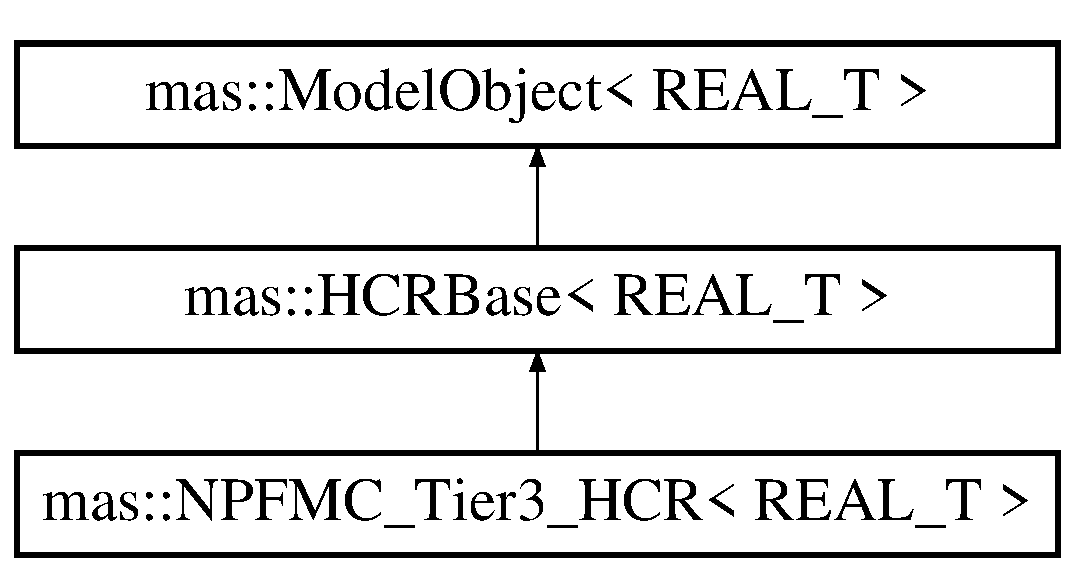
\includegraphics[height=3.000000cm]{structmas_1_1_n_p_f_m_c___tier3___h_c_r}
\end{center}
\end{figure}
\subsection*{Public Types}
\begin{DoxyCompactItemize}
\item 
typedef \hyperlink{structmas_1_1_variable_trait}{Variable\-Trait}$<$ R\-E\-A\-L\-\_\-\-T $>$\\*
\-::\hyperlink{structmas_1_1_n_p_f_m_c___tier3___h_c_r_a255d04535c769276bb11c0a7e003d775}{variable} \hyperlink{structmas_1_1_n_p_f_m_c___tier3___h_c_r_a255d04535c769276bb11c0a7e003d775}{variable}
\end{DoxyCompactItemize}
\subsection*{Public Member Functions}
\begin{DoxyCompactItemize}
\item 
std\-::pair$<$ \hyperlink{structmas_1_1_n_p_f_m_c___tier3___h_c_r_a255d04535c769276bb11c0a7e003d775}{variable}, \hyperlink{structmas_1_1_n_p_f_m_c___tier3___h_c_r_a255d04535c769276bb11c0a7e003d775}{variable} $>$ \hyperlink{structmas_1_1_n_p_f_m_c___tier3___h_c_r_add1b49da6fec0371e54e5b729ba249fc}{Calculate\-Fat\-S\-P\-Rfraction} (const \hyperlink{structmas_1_1_n_p_f_m_c___tier3___h_c_r_a255d04535c769276bb11c0a7e003d775}{variable} \&spr\-\_\-fraction, const std\-::vector$<$ \hyperlink{structmas_1_1_n_p_f_m_c___tier3___h_c_r_a255d04535c769276bb11c0a7e003d775}{variable} $>$ \&fsh\-\_\-sel, const \hyperlink{structmas_1_1_area_population_info}{mas\-::\-Area\-Population\-Info}$<$ R\-E\-A\-L\-\_\-\-T $>$ \&api)
\item 
\hyperlink{structmas_1_1_n_p_f_m_c___tier3___h_c_r_a255d04535c769276bb11c0a7e003d775}{variable} \hyperlink{structmas_1_1_n_p_f_m_c___tier3___h_c_r_a41b3cf631b6c4d52c3539853efbbcf18}{Calculate\-S\-Bat\-F} (const \hyperlink{structmas_1_1_n_p_f_m_c___tier3___h_c_r_a255d04535c769276bb11c0a7e003d775}{variable} \&trial\-F, const std\-::vector$<$ \hyperlink{structmas_1_1_n_p_f_m_c___tier3___h_c_r_a255d04535c769276bb11c0a7e003d775}{variable} $>$ \&fsh\-\_\-sel, const \hyperlink{structmas_1_1_area_population_info}{mas\-::\-Area\-Population\-Info}$<$ R\-E\-A\-L\-\_\-\-T $>$ \&api)
\item 
const std\-::tuple$<$ \hyperlink{structmas_1_1_n_p_f_m_c___tier3___h_c_r_a255d04535c769276bb11c0a7e003d775}{variable}, \\*
\hyperlink{structmas_1_1_n_p_f_m_c___tier3___h_c_r_a255d04535c769276bb11c0a7e003d775}{variable}, \hyperlink{structmas_1_1_n_p_f_m_c___tier3___h_c_r_a255d04535c769276bb11c0a7e003d775}{variable}, \hyperlink{structmas_1_1_n_p_f_m_c___tier3___h_c_r_a255d04535c769276bb11c0a7e003d775}{variable} $>$ \hyperlink{structmas_1_1_n_p_f_m_c___tier3___h_c_r_af95105dd7d8a4a47ab028c34b35640ff}{Evaluate} (const int \&year, const \hyperlink{structmas_1_1_area_population_info}{mas\-::\-Area\-Population\-Info}$<$ R\-E\-A\-L\-\_\-\-T $>$ \&api\-\_\-males, const \hyperlink{structmas_1_1_area_population_info}{mas\-::\-Area\-Population\-Info}$<$ R\-E\-A\-L\-\_\-\-T $>$ \&api\-\_\-females)
\item 
const std\-::string \hyperlink{structmas_1_1_n_p_f_m_c___tier3___h_c_r_a1f7d15c97821f987d8b8ef1a2c8099a5}{Name} ()
\end{DoxyCompactItemize}
\subsection*{Public Attributes}
\begin{DoxyCompactItemize}
\item 
std\-::pair$<$ \hyperlink{structmas_1_1_n_p_f_m_c___tier3___h_c_r_a255d04535c769276bb11c0a7e003d775}{variable}, \hyperlink{structmas_1_1_n_p_f_m_c___tier3___h_c_r_a255d04535c769276bb11c0a7e003d775}{variable} $>$ \hyperlink{structmas_1_1_n_p_f_m_c___tier3___h_c_r_a8686f8a9896d1a62e069008416bdb1c4}{B\-R\-P100}
\item 
std\-::pair$<$ \hyperlink{structmas_1_1_n_p_f_m_c___tier3___h_c_r_a255d04535c769276bb11c0a7e003d775}{variable}, \hyperlink{structmas_1_1_n_p_f_m_c___tier3___h_c_r_a255d04535c769276bb11c0a7e003d775}{variable} $>$ \hyperlink{structmas_1_1_n_p_f_m_c___tier3___h_c_r_af0fb6ed0057002e7e92172f725ad6534}{B\-R\-P40}
\item 
std\-::pair$<$ \hyperlink{structmas_1_1_n_p_f_m_c___tier3___h_c_r_a255d04535c769276bb11c0a7e003d775}{variable}, \hyperlink{structmas_1_1_n_p_f_m_c___tier3___h_c_r_a255d04535c769276bb11c0a7e003d775}{variable} $>$ \hyperlink{structmas_1_1_n_p_f_m_c___tier3___h_c_r_a6962cd915784729c57541f02694a71b0}{B\-R\-P35}
\item 
std\-::pair$<$ \hyperlink{structmas_1_1_n_p_f_m_c___tier3___h_c_r_a255d04535c769276bb11c0a7e003d775}{variable}, \hyperlink{structmas_1_1_n_p_f_m_c___tier3___h_c_r_a255d04535c769276bb11c0a7e003d775}{variable} $>$ \hyperlink{structmas_1_1_n_p_f_m_c___tier3___h_c_r_a6dbb8dfb2765b64d3fb0ba474ab24003}{B\-R\-P20}
\item 
std\-::pair$<$ \hyperlink{structmas_1_1_n_p_f_m_c___tier3___h_c_r_a255d04535c769276bb11c0a7e003d775}{variable}, \hyperlink{structmas_1_1_n_p_f_m_c___tier3___h_c_r_a255d04535c769276bb11c0a7e003d775}{variable} $>$ \hyperlink{structmas_1_1_n_p_f_m_c___tier3___h_c_r_a9885e5cfad14aa0b9ed0867998af775c}{B\-R\-P05}
\item 
\hyperlink{structmas_1_1_n_p_f_m_c___tier3___h_c_r_a255d04535c769276bb11c0a7e003d775}{variable} \hyperlink{structmas_1_1_n_p_f_m_c___tier3___h_c_r_ae91373c1b4216cd93126615e881b9d92}{F\-\_\-\-A\-B\-C}
\item 
\hyperlink{structmas_1_1_n_p_f_m_c___tier3___h_c_r_a255d04535c769276bb11c0a7e003d775}{variable} \hyperlink{structmas_1_1_n_p_f_m_c___tier3___h_c_r_a1360399be1b30447d5dcfbbb57318ec4}{A\-B\-C}
\item 
\hyperlink{structmas_1_1_n_p_f_m_c___tier3___h_c_r_a255d04535c769276bb11c0a7e003d775}{variable} \hyperlink{structmas_1_1_n_p_f_m_c___tier3___h_c_r_a5dd5ec6b7ffd1eae4a0b32cf062cf51f}{F\-\_\-\-O\-F\-L}
\item 
\hyperlink{structmas_1_1_n_p_f_m_c___tier3___h_c_r_a255d04535c769276bb11c0a7e003d775}{variable} \hyperlink{structmas_1_1_n_p_f_m_c___tier3___h_c_r_aea706f530b4d4d6ec4df8a5aead87890}{O\-F\-L}
\end{DoxyCompactItemize}


\subsection{Detailed Description}
\subsubsection*{template$<$typename R\-E\-A\-L\-\_\-\-T$>$struct mas\-::\-N\-P\-F\-M\-C\-\_\-\-Tier3\-\_\-\-H\-C\-R$<$ R\-E\-A\-L\-\_\-\-T $>$}



Definition at line 66 of file Harvest\-Control\-Rule.\-hpp.



\subsection{Member Typedef Documentation}
\hypertarget{structmas_1_1_n_p_f_m_c___tier3___h_c_r_a255d04535c769276bb11c0a7e003d775}{\index{mas\-::\-N\-P\-F\-M\-C\-\_\-\-Tier3\-\_\-\-H\-C\-R@{mas\-::\-N\-P\-F\-M\-C\-\_\-\-Tier3\-\_\-\-H\-C\-R}!variable@{variable}}
\index{variable@{variable}!mas::NPFMC_Tier3_HCR@{mas\-::\-N\-P\-F\-M\-C\-\_\-\-Tier3\-\_\-\-H\-C\-R}}
\subsubsection[{variable}]{\setlength{\rightskip}{0pt plus 5cm}template$<$typename R\-E\-A\-L\-\_\-\-T $>$ typedef {\bf Variable\-Trait}$<$R\-E\-A\-L\-\_\-\-T$>$\-::{\bf variable} {\bf mas\-::\-N\-P\-F\-M\-C\-\_\-\-Tier3\-\_\-\-H\-C\-R}$<$ R\-E\-A\-L\-\_\-\-T $>$\-::{\bf variable}}}\label{structmas_1_1_n_p_f_m_c___tier3___h_c_r_a255d04535c769276bb11c0a7e003d775}


Definition at line 68 of file Harvest\-Control\-Rule.\-hpp.



\subsection{Member Function Documentation}
\hypertarget{structmas_1_1_n_p_f_m_c___tier3___h_c_r_add1b49da6fec0371e54e5b729ba249fc}{\index{mas\-::\-N\-P\-F\-M\-C\-\_\-\-Tier3\-\_\-\-H\-C\-R@{mas\-::\-N\-P\-F\-M\-C\-\_\-\-Tier3\-\_\-\-H\-C\-R}!Calculate\-Fat\-S\-P\-Rfraction@{Calculate\-Fat\-S\-P\-Rfraction}}
\index{Calculate\-Fat\-S\-P\-Rfraction@{Calculate\-Fat\-S\-P\-Rfraction}!mas::NPFMC_Tier3_HCR@{mas\-::\-N\-P\-F\-M\-C\-\_\-\-Tier3\-\_\-\-H\-C\-R}}
\subsubsection[{Calculate\-Fat\-S\-P\-Rfraction}]{\setlength{\rightskip}{0pt plus 5cm}template$<$typename R\-E\-A\-L\-\_\-\-T $>$ std\-::pair$<${\bf variable}, {\bf variable}$>$ {\bf mas\-::\-N\-P\-F\-M\-C\-\_\-\-Tier3\-\_\-\-H\-C\-R}$<$ R\-E\-A\-L\-\_\-\-T $>$\-::Calculate\-Fat\-S\-P\-Rfraction (
\begin{DoxyParamCaption}
\item[{const {\bf variable} \&}]{spr\-\_\-fraction, }
\item[{const std\-::vector$<$ {\bf variable} $>$ \&}]{fsh\-\_\-sel, }
\item[{const {\bf mas\-::\-Area\-Population\-Info}$<$ R\-E\-A\-L\-\_\-\-T $>$ \&}]{api}
\end{DoxyParamCaption}
)\hspace{0.3cm}{\ttfamily [inline]}}}\label{structmas_1_1_n_p_f_m_c___tier3___h_c_r_add1b49da6fec0371e54e5b729ba249fc}


Definition at line 76 of file Harvest\-Control\-Rule.\-hpp.

\hypertarget{structmas_1_1_n_p_f_m_c___tier3___h_c_r_a41b3cf631b6c4d52c3539853efbbcf18}{\index{mas\-::\-N\-P\-F\-M\-C\-\_\-\-Tier3\-\_\-\-H\-C\-R@{mas\-::\-N\-P\-F\-M\-C\-\_\-\-Tier3\-\_\-\-H\-C\-R}!Calculate\-S\-Bat\-F@{Calculate\-S\-Bat\-F}}
\index{Calculate\-S\-Bat\-F@{Calculate\-S\-Bat\-F}!mas::NPFMC_Tier3_HCR@{mas\-::\-N\-P\-F\-M\-C\-\_\-\-Tier3\-\_\-\-H\-C\-R}}
\subsubsection[{Calculate\-S\-Bat\-F}]{\setlength{\rightskip}{0pt plus 5cm}template$<$typename R\-E\-A\-L\-\_\-\-T $>$ {\bf variable} {\bf mas\-::\-N\-P\-F\-M\-C\-\_\-\-Tier3\-\_\-\-H\-C\-R}$<$ R\-E\-A\-L\-\_\-\-T $>$\-::Calculate\-S\-Bat\-F (
\begin{DoxyParamCaption}
\item[{const {\bf variable} \&}]{trial\-F, }
\item[{const std\-::vector$<$ {\bf variable} $>$ \&}]{fsh\-\_\-sel, }
\item[{const {\bf mas\-::\-Area\-Population\-Info}$<$ R\-E\-A\-L\-\_\-\-T $>$ \&}]{api}
\end{DoxyParamCaption}
)\hspace{0.3cm}{\ttfamily [inline]}}}\label{structmas_1_1_n_p_f_m_c___tier3___h_c_r_a41b3cf631b6c4d52c3539853efbbcf18}


Definition at line 117 of file Harvest\-Control\-Rule.\-hpp.

\hypertarget{structmas_1_1_n_p_f_m_c___tier3___h_c_r_af95105dd7d8a4a47ab028c34b35640ff}{\index{mas\-::\-N\-P\-F\-M\-C\-\_\-\-Tier3\-\_\-\-H\-C\-R@{mas\-::\-N\-P\-F\-M\-C\-\_\-\-Tier3\-\_\-\-H\-C\-R}!Evaluate@{Evaluate}}
\index{Evaluate@{Evaluate}!mas::NPFMC_Tier3_HCR@{mas\-::\-N\-P\-F\-M\-C\-\_\-\-Tier3\-\_\-\-H\-C\-R}}
\subsubsection[{Evaluate}]{\setlength{\rightskip}{0pt plus 5cm}template$<$typename R\-E\-A\-L\-\_\-\-T $>$ const std\-::tuple$<${\bf variable}, {\bf variable}, {\bf variable}, {\bf variable}$>$ {\bf mas\-::\-N\-P\-F\-M\-C\-\_\-\-Tier3\-\_\-\-H\-C\-R}$<$ R\-E\-A\-L\-\_\-\-T $>$\-::Evaluate (
\begin{DoxyParamCaption}
\item[{const int \&}]{year, }
\item[{const {\bf mas\-::\-Area\-Population\-Info}$<$ R\-E\-A\-L\-\_\-\-T $>$ \&}]{api\-\_\-males, }
\item[{const {\bf mas\-::\-Area\-Population\-Info}$<$ R\-E\-A\-L\-\_\-\-T $>$ \&}]{api\-\_\-females}
\end{DoxyParamCaption}
)\hspace{0.3cm}{\ttfamily [inline]}, {\ttfamily [virtual]}}}\label{structmas_1_1_n_p_f_m_c___tier3___h_c_r_af95105dd7d8a4a47ab028c34b35640ff}


Implements \hyperlink{structmas_1_1_h_c_r_base_a3d923b3276f10e4c7938abde6a134291}{mas\-::\-H\-C\-R\-Base$<$ R\-E\-A\-L\-\_\-\-T $>$}.



Definition at line 148 of file Harvest\-Control\-Rule.\-hpp.

\hypertarget{structmas_1_1_n_p_f_m_c___tier3___h_c_r_a1f7d15c97821f987d8b8ef1a2c8099a5}{\index{mas\-::\-N\-P\-F\-M\-C\-\_\-\-Tier3\-\_\-\-H\-C\-R@{mas\-::\-N\-P\-F\-M\-C\-\_\-\-Tier3\-\_\-\-H\-C\-R}!Name@{Name}}
\index{Name@{Name}!mas::NPFMC_Tier3_HCR@{mas\-::\-N\-P\-F\-M\-C\-\_\-\-Tier3\-\_\-\-H\-C\-R}}
\subsubsection[{Name}]{\setlength{\rightskip}{0pt plus 5cm}template$<$typename R\-E\-A\-L\-\_\-\-T $>$ const std\-::string {\bf mas\-::\-N\-P\-F\-M\-C\-\_\-\-Tier3\-\_\-\-H\-C\-R}$<$ R\-E\-A\-L\-\_\-\-T $>$\-::Name (
\begin{DoxyParamCaption}
{}
\end{DoxyParamCaption}
)\hspace{0.3cm}{\ttfamily [inline]}, {\ttfamily [virtual]}}}\label{structmas_1_1_n_p_f_m_c___tier3___h_c_r_a1f7d15c97821f987d8b8ef1a2c8099a5}


Reimplemented from \hyperlink{structmas_1_1_h_c_r_base_a3f1aa4335bee8d9225776ca5212e1085}{mas\-::\-H\-C\-R\-Base$<$ R\-E\-A\-L\-\_\-\-T $>$}.



Definition at line 280 of file Harvest\-Control\-Rule.\-hpp.



\subsection{Member Data Documentation}
\hypertarget{structmas_1_1_n_p_f_m_c___tier3___h_c_r_a1360399be1b30447d5dcfbbb57318ec4}{\index{mas\-::\-N\-P\-F\-M\-C\-\_\-\-Tier3\-\_\-\-H\-C\-R@{mas\-::\-N\-P\-F\-M\-C\-\_\-\-Tier3\-\_\-\-H\-C\-R}!A\-B\-C@{A\-B\-C}}
\index{A\-B\-C@{A\-B\-C}!mas::NPFMC_Tier3_HCR@{mas\-::\-N\-P\-F\-M\-C\-\_\-\-Tier3\-\_\-\-H\-C\-R}}
\subsubsection[{A\-B\-C}]{\setlength{\rightskip}{0pt plus 5cm}template$<$typename R\-E\-A\-L\-\_\-\-T $>$ {\bf variable} {\bf mas\-::\-N\-P\-F\-M\-C\-\_\-\-Tier3\-\_\-\-H\-C\-R}$<$ R\-E\-A\-L\-\_\-\-T $>$\-::A\-B\-C}}\label{structmas_1_1_n_p_f_m_c___tier3___h_c_r_a1360399be1b30447d5dcfbbb57318ec4}


Definition at line 71 of file Harvest\-Control\-Rule.\-hpp.

\hypertarget{structmas_1_1_n_p_f_m_c___tier3___h_c_r_a9885e5cfad14aa0b9ed0867998af775c}{\index{mas\-::\-N\-P\-F\-M\-C\-\_\-\-Tier3\-\_\-\-H\-C\-R@{mas\-::\-N\-P\-F\-M\-C\-\_\-\-Tier3\-\_\-\-H\-C\-R}!B\-R\-P05@{B\-R\-P05}}
\index{B\-R\-P05@{B\-R\-P05}!mas::NPFMC_Tier3_HCR@{mas\-::\-N\-P\-F\-M\-C\-\_\-\-Tier3\-\_\-\-H\-C\-R}}
\subsubsection[{B\-R\-P05}]{\setlength{\rightskip}{0pt plus 5cm}template$<$typename R\-E\-A\-L\-\_\-\-T $>$ std\-::pair$<${\bf variable}, {\bf variable}$>$ {\bf mas\-::\-N\-P\-F\-M\-C\-\_\-\-Tier3\-\_\-\-H\-C\-R}$<$ R\-E\-A\-L\-\_\-\-T $>$\-::B\-R\-P05}}\label{structmas_1_1_n_p_f_m_c___tier3___h_c_r_a9885e5cfad14aa0b9ed0867998af775c}


Definition at line 70 of file Harvest\-Control\-Rule.\-hpp.

\hypertarget{structmas_1_1_n_p_f_m_c___tier3___h_c_r_a8686f8a9896d1a62e069008416bdb1c4}{\index{mas\-::\-N\-P\-F\-M\-C\-\_\-\-Tier3\-\_\-\-H\-C\-R@{mas\-::\-N\-P\-F\-M\-C\-\_\-\-Tier3\-\_\-\-H\-C\-R}!B\-R\-P100@{B\-R\-P100}}
\index{B\-R\-P100@{B\-R\-P100}!mas::NPFMC_Tier3_HCR@{mas\-::\-N\-P\-F\-M\-C\-\_\-\-Tier3\-\_\-\-H\-C\-R}}
\subsubsection[{B\-R\-P100}]{\setlength{\rightskip}{0pt plus 5cm}template$<$typename R\-E\-A\-L\-\_\-\-T $>$ std\-::pair$<${\bf variable}, {\bf variable}$>$ {\bf mas\-::\-N\-P\-F\-M\-C\-\_\-\-Tier3\-\_\-\-H\-C\-R}$<$ R\-E\-A\-L\-\_\-\-T $>$\-::B\-R\-P100}}\label{structmas_1_1_n_p_f_m_c___tier3___h_c_r_a8686f8a9896d1a62e069008416bdb1c4}


Definition at line 70 of file Harvest\-Control\-Rule.\-hpp.

\hypertarget{structmas_1_1_n_p_f_m_c___tier3___h_c_r_a6dbb8dfb2765b64d3fb0ba474ab24003}{\index{mas\-::\-N\-P\-F\-M\-C\-\_\-\-Tier3\-\_\-\-H\-C\-R@{mas\-::\-N\-P\-F\-M\-C\-\_\-\-Tier3\-\_\-\-H\-C\-R}!B\-R\-P20@{B\-R\-P20}}
\index{B\-R\-P20@{B\-R\-P20}!mas::NPFMC_Tier3_HCR@{mas\-::\-N\-P\-F\-M\-C\-\_\-\-Tier3\-\_\-\-H\-C\-R}}
\subsubsection[{B\-R\-P20}]{\setlength{\rightskip}{0pt plus 5cm}template$<$typename R\-E\-A\-L\-\_\-\-T $>$ std\-::pair$<${\bf variable}, {\bf variable}$>$ {\bf mas\-::\-N\-P\-F\-M\-C\-\_\-\-Tier3\-\_\-\-H\-C\-R}$<$ R\-E\-A\-L\-\_\-\-T $>$\-::B\-R\-P20}}\label{structmas_1_1_n_p_f_m_c___tier3___h_c_r_a6dbb8dfb2765b64d3fb0ba474ab24003}


Definition at line 70 of file Harvest\-Control\-Rule.\-hpp.

\hypertarget{structmas_1_1_n_p_f_m_c___tier3___h_c_r_a6962cd915784729c57541f02694a71b0}{\index{mas\-::\-N\-P\-F\-M\-C\-\_\-\-Tier3\-\_\-\-H\-C\-R@{mas\-::\-N\-P\-F\-M\-C\-\_\-\-Tier3\-\_\-\-H\-C\-R}!B\-R\-P35@{B\-R\-P35}}
\index{B\-R\-P35@{B\-R\-P35}!mas::NPFMC_Tier3_HCR@{mas\-::\-N\-P\-F\-M\-C\-\_\-\-Tier3\-\_\-\-H\-C\-R}}
\subsubsection[{B\-R\-P35}]{\setlength{\rightskip}{0pt plus 5cm}template$<$typename R\-E\-A\-L\-\_\-\-T $>$ std\-::pair$<${\bf variable}, {\bf variable}$>$ {\bf mas\-::\-N\-P\-F\-M\-C\-\_\-\-Tier3\-\_\-\-H\-C\-R}$<$ R\-E\-A\-L\-\_\-\-T $>$\-::B\-R\-P35}}\label{structmas_1_1_n_p_f_m_c___tier3___h_c_r_a6962cd915784729c57541f02694a71b0}


Definition at line 70 of file Harvest\-Control\-Rule.\-hpp.

\hypertarget{structmas_1_1_n_p_f_m_c___tier3___h_c_r_af0fb6ed0057002e7e92172f725ad6534}{\index{mas\-::\-N\-P\-F\-M\-C\-\_\-\-Tier3\-\_\-\-H\-C\-R@{mas\-::\-N\-P\-F\-M\-C\-\_\-\-Tier3\-\_\-\-H\-C\-R}!B\-R\-P40@{B\-R\-P40}}
\index{B\-R\-P40@{B\-R\-P40}!mas::NPFMC_Tier3_HCR@{mas\-::\-N\-P\-F\-M\-C\-\_\-\-Tier3\-\_\-\-H\-C\-R}}
\subsubsection[{B\-R\-P40}]{\setlength{\rightskip}{0pt plus 5cm}template$<$typename R\-E\-A\-L\-\_\-\-T $>$ std\-::pair$<${\bf variable}, {\bf variable}$>$ {\bf mas\-::\-N\-P\-F\-M\-C\-\_\-\-Tier3\-\_\-\-H\-C\-R}$<$ R\-E\-A\-L\-\_\-\-T $>$\-::B\-R\-P40}}\label{structmas_1_1_n_p_f_m_c___tier3___h_c_r_af0fb6ed0057002e7e92172f725ad6534}


Definition at line 70 of file Harvest\-Control\-Rule.\-hpp.

\hypertarget{structmas_1_1_n_p_f_m_c___tier3___h_c_r_ae91373c1b4216cd93126615e881b9d92}{\index{mas\-::\-N\-P\-F\-M\-C\-\_\-\-Tier3\-\_\-\-H\-C\-R@{mas\-::\-N\-P\-F\-M\-C\-\_\-\-Tier3\-\_\-\-H\-C\-R}!F\-\_\-\-A\-B\-C@{F\-\_\-\-A\-B\-C}}
\index{F\-\_\-\-A\-B\-C@{F\-\_\-\-A\-B\-C}!mas::NPFMC_Tier3_HCR@{mas\-::\-N\-P\-F\-M\-C\-\_\-\-Tier3\-\_\-\-H\-C\-R}}
\subsubsection[{F\-\_\-\-A\-B\-C}]{\setlength{\rightskip}{0pt plus 5cm}template$<$typename R\-E\-A\-L\-\_\-\-T $>$ {\bf variable} {\bf mas\-::\-N\-P\-F\-M\-C\-\_\-\-Tier3\-\_\-\-H\-C\-R}$<$ R\-E\-A\-L\-\_\-\-T $>$\-::F\-\_\-\-A\-B\-C}}\label{structmas_1_1_n_p_f_m_c___tier3___h_c_r_ae91373c1b4216cd93126615e881b9d92}


Definition at line 71 of file Harvest\-Control\-Rule.\-hpp.

\hypertarget{structmas_1_1_n_p_f_m_c___tier3___h_c_r_a5dd5ec6b7ffd1eae4a0b32cf062cf51f}{\index{mas\-::\-N\-P\-F\-M\-C\-\_\-\-Tier3\-\_\-\-H\-C\-R@{mas\-::\-N\-P\-F\-M\-C\-\_\-\-Tier3\-\_\-\-H\-C\-R}!F\-\_\-\-O\-F\-L@{F\-\_\-\-O\-F\-L}}
\index{F\-\_\-\-O\-F\-L@{F\-\_\-\-O\-F\-L}!mas::NPFMC_Tier3_HCR@{mas\-::\-N\-P\-F\-M\-C\-\_\-\-Tier3\-\_\-\-H\-C\-R}}
\subsubsection[{F\-\_\-\-O\-F\-L}]{\setlength{\rightskip}{0pt plus 5cm}template$<$typename R\-E\-A\-L\-\_\-\-T $>$ {\bf variable} {\bf mas\-::\-N\-P\-F\-M\-C\-\_\-\-Tier3\-\_\-\-H\-C\-R}$<$ R\-E\-A\-L\-\_\-\-T $>$\-::F\-\_\-\-O\-F\-L}}\label{structmas_1_1_n_p_f_m_c___tier3___h_c_r_a5dd5ec6b7ffd1eae4a0b32cf062cf51f}


Definition at line 71 of file Harvest\-Control\-Rule.\-hpp.

\hypertarget{structmas_1_1_n_p_f_m_c___tier3___h_c_r_aea706f530b4d4d6ec4df8a5aead87890}{\index{mas\-::\-N\-P\-F\-M\-C\-\_\-\-Tier3\-\_\-\-H\-C\-R@{mas\-::\-N\-P\-F\-M\-C\-\_\-\-Tier3\-\_\-\-H\-C\-R}!O\-F\-L@{O\-F\-L}}
\index{O\-F\-L@{O\-F\-L}!mas::NPFMC_Tier3_HCR@{mas\-::\-N\-P\-F\-M\-C\-\_\-\-Tier3\-\_\-\-H\-C\-R}}
\subsubsection[{O\-F\-L}]{\setlength{\rightskip}{0pt plus 5cm}template$<$typename R\-E\-A\-L\-\_\-\-T $>$ {\bf variable} {\bf mas\-::\-N\-P\-F\-M\-C\-\_\-\-Tier3\-\_\-\-H\-C\-R}$<$ R\-E\-A\-L\-\_\-\-T $>$\-::O\-F\-L}}\label{structmas_1_1_n_p_f_m_c___tier3___h_c_r_aea706f530b4d4d6ec4df8a5aead87890}


Definition at line 71 of file Harvest\-Control\-Rule.\-hpp.



The documentation for this struct was generated from the following file\-:\begin{DoxyCompactItemize}
\item 
/home/oppy/\-Net\-Beans\-Projects/mas/\hyperlink{_harvest_control_rule_8hpp}{Harvest\-Control\-Rule.\-hpp}\end{DoxyCompactItemize}

\hypertarget{struct_options}{\section{Options$<$ T $>$ Struct Template Reference}
\label{struct_options}\index{Options$<$ T $>$@{Options$<$ T $>$}}
}
\subsection*{Public Attributes}
\begin{DoxyCompactItemize}
\item 
\hyperlink{main_8cpp_a85135cb2967cc1e21d0e2e96b125c071}{Minimizer} \hyperlink{struct_options_ab1527f6ea213b470e60f0bfb673e6626}{minimizer} = \hyperlink{main_8cpp_a85135cb2967cc1e21d0e2e96b125c071a8aa2d5dcc79c3457a8be44efe68348ad}{L\-B\-F\-G\-S}
\item 
T \hyperlink{struct_options_ac2dba4b15b871ca36825ec4c2fc38753}{tol} = static\-\_\-cast$<$T$>$ (1e-\/4)
\item 
int \hyperlink{struct_options_a38be912695cadd656ec4638440eb452e}{min\-\_\-iter} = 5000
\item 
int \hyperlink{struct_options_a65ca6536c995fd09207c19b26d6a657f}{iprint} = 10
\item 
\hyperlink{main_8cpp_a92d0159edd3899a97773bf080589435c}{M\-C\-M\-C} \hyperlink{struct_options_a658501e489501c4ce7c139257ee57d93}{mcmc} = \hyperlink{main_8cpp_a92d0159edd3899a97773bf080589435ca79bc3feff3a4c676991ac57a8e9764ab}{M\-H}
\item 
int \hyperlink{struct_options_a40e40c4cbdb83403f52dbecc0fe07749}{boot\-\_\-strap} = 5000
\item 
int \hyperlink{struct_options_a5f067cf738d25bcd5babfcfa5b109509}{mcmc\-\_\-iter} = 5000
\item 
std\-::string \hyperlink{struct_options_a1ac9c3e29359a31236632434946f379c}{config} = \char`\"{}N\-A\char`\"{}
\item 
std\-::string \hyperlink{struct_options_af07888a17b99d02ba62574edc34ccaee}{data} = \char`\"{}N\-A\char`\"{}
\item 
std\-::string \hyperlink{struct_options_ac0336cacd551ef3176e4e133a179fb8b}{output\-\_\-directory} = \char`\"{}N\-A\char`\"{}
\end{DoxyCompactItemize}


\subsection{Detailed Description}
\subsubsection*{template$<$typename T$>$struct Options$<$ T $>$}



Definition at line 148 of file main.\-cpp.



\subsection{Member Data Documentation}
\hypertarget{struct_options_a40e40c4cbdb83403f52dbecc0fe07749}{\index{Options@{Options}!boot\-\_\-strap@{boot\-\_\-strap}}
\index{boot\-\_\-strap@{boot\-\_\-strap}!Options@{Options}}
\subsubsection[{boot\-\_\-strap}]{\setlength{\rightskip}{0pt plus 5cm}template$<$typename T$>$ int {\bf Options}$<$ T $>$\-::boot\-\_\-strap = 5000}}\label{struct_options_a40e40c4cbdb83403f52dbecc0fe07749}


Definition at line 157 of file main.\-cpp.

\hypertarget{struct_options_a1ac9c3e29359a31236632434946f379c}{\index{Options@{Options}!config@{config}}
\index{config@{config}!Options@{Options}}
\subsubsection[{config}]{\setlength{\rightskip}{0pt plus 5cm}template$<$typename T$>$ std\-::string {\bf Options}$<$ T $>$\-::config = \char`\"{}N\-A\char`\"{}}}\label{struct_options_a1ac9c3e29359a31236632434946f379c}


Definition at line 159 of file main.\-cpp.

\hypertarget{struct_options_af07888a17b99d02ba62574edc34ccaee}{\index{Options@{Options}!data@{data}}
\index{data@{data}!Options@{Options}}
\subsubsection[{data}]{\setlength{\rightskip}{0pt plus 5cm}template$<$typename T$>$ std\-::string {\bf Options}$<$ T $>$\-::data = \char`\"{}N\-A\char`\"{}}}\label{struct_options_af07888a17b99d02ba62574edc34ccaee}


Definition at line 160 of file main.\-cpp.

\hypertarget{struct_options_a65ca6536c995fd09207c19b26d6a657f}{\index{Options@{Options}!iprint@{iprint}}
\index{iprint@{iprint}!Options@{Options}}
\subsubsection[{iprint}]{\setlength{\rightskip}{0pt plus 5cm}template$<$typename T$>$ int {\bf Options}$<$ T $>$\-::iprint = 10}}\label{struct_options_a65ca6536c995fd09207c19b26d6a657f}


Definition at line 153 of file main.\-cpp.

\hypertarget{struct_options_a658501e489501c4ce7c139257ee57d93}{\index{Options@{Options}!mcmc@{mcmc}}
\index{mcmc@{mcmc}!Options@{Options}}
\subsubsection[{mcmc}]{\setlength{\rightskip}{0pt plus 5cm}template$<$typename T$>$ {\bf M\-C\-M\-C} {\bf Options}$<$ T $>$\-::mcmc = {\bf M\-H}}}\label{struct_options_a658501e489501c4ce7c139257ee57d93}


Definition at line 156 of file main.\-cpp.

\hypertarget{struct_options_a5f067cf738d25bcd5babfcfa5b109509}{\index{Options@{Options}!mcmc\-\_\-iter@{mcmc\-\_\-iter}}
\index{mcmc\-\_\-iter@{mcmc\-\_\-iter}!Options@{Options}}
\subsubsection[{mcmc\-\_\-iter}]{\setlength{\rightskip}{0pt plus 5cm}template$<$typename T$>$ int {\bf Options}$<$ T $>$\-::mcmc\-\_\-iter = 5000}}\label{struct_options_a5f067cf738d25bcd5babfcfa5b109509}


Definition at line 158 of file main.\-cpp.

\hypertarget{struct_options_a38be912695cadd656ec4638440eb452e}{\index{Options@{Options}!min\-\_\-iter@{min\-\_\-iter}}
\index{min\-\_\-iter@{min\-\_\-iter}!Options@{Options}}
\subsubsection[{min\-\_\-iter}]{\setlength{\rightskip}{0pt plus 5cm}template$<$typename T$>$ int {\bf Options}$<$ T $>$\-::min\-\_\-iter = 5000}}\label{struct_options_a38be912695cadd656ec4638440eb452e}


Definition at line 152 of file main.\-cpp.

\hypertarget{struct_options_ab1527f6ea213b470e60f0bfb673e6626}{\index{Options@{Options}!minimizer@{minimizer}}
\index{minimizer@{minimizer}!Options@{Options}}
\subsubsection[{minimizer}]{\setlength{\rightskip}{0pt plus 5cm}template$<$typename T$>$ {\bf Minimizer} {\bf Options}$<$ T $>$\-::minimizer = {\bf L\-B\-F\-G\-S}}}\label{struct_options_ab1527f6ea213b470e60f0bfb673e6626}


Definition at line 150 of file main.\-cpp.

\hypertarget{struct_options_ac0336cacd551ef3176e4e133a179fb8b}{\index{Options@{Options}!output\-\_\-directory@{output\-\_\-directory}}
\index{output\-\_\-directory@{output\-\_\-directory}!Options@{Options}}
\subsubsection[{output\-\_\-directory}]{\setlength{\rightskip}{0pt plus 5cm}template$<$typename T$>$ std\-::string {\bf Options}$<$ T $>$\-::output\-\_\-directory = \char`\"{}N\-A\char`\"{}}}\label{struct_options_ac0336cacd551ef3176e4e133a179fb8b}


Definition at line 161 of file main.\-cpp.

\hypertarget{struct_options_ac2dba4b15b871ca36825ec4c2fc38753}{\index{Options@{Options}!tol@{tol}}
\index{tol@{tol}!Options@{Options}}
\subsubsection[{tol}]{\setlength{\rightskip}{0pt plus 5cm}template$<$typename T$>$ T {\bf Options}$<$ T $>$\-::tol = static\-\_\-cast$<$T$>$ (1e-\/4)}}\label{struct_options_ac2dba4b15b871ca36825ec4c2fc38753}


Definition at line 151 of file main.\-cpp.



The documentation for this struct was generated from the following file\-:\begin{DoxyCompactItemize}
\item 
/home/oppy/\-Net\-Beans\-Projects/mas/\hyperlink{main_8cpp}{main.\-cpp}\end{DoxyCompactItemize}

\hypertarget{structmas_1_1_p_f_m_c___h_c_r}{\section{mas\-:\-:P\-F\-M\-C\-\_\-\-H\-C\-R$<$ R\-E\-A\-L\-\_\-\-T $>$ Struct Template Reference}
\label{structmas_1_1_p_f_m_c___h_c_r}\index{mas\-::\-P\-F\-M\-C\-\_\-\-H\-C\-R$<$ R\-E\-A\-L\-\_\-\-T $>$@{mas\-::\-P\-F\-M\-C\-\_\-\-H\-C\-R$<$ R\-E\-A\-L\-\_\-\-T $>$}}
}


{\ttfamily \#include $<$Harvest\-Control\-Rule.\-hpp$>$}

Inheritance diagram for mas\-:\-:P\-F\-M\-C\-\_\-\-H\-C\-R$<$ R\-E\-A\-L\-\_\-\-T $>$\-:\begin{figure}[H]
\begin{center}
\leavevmode
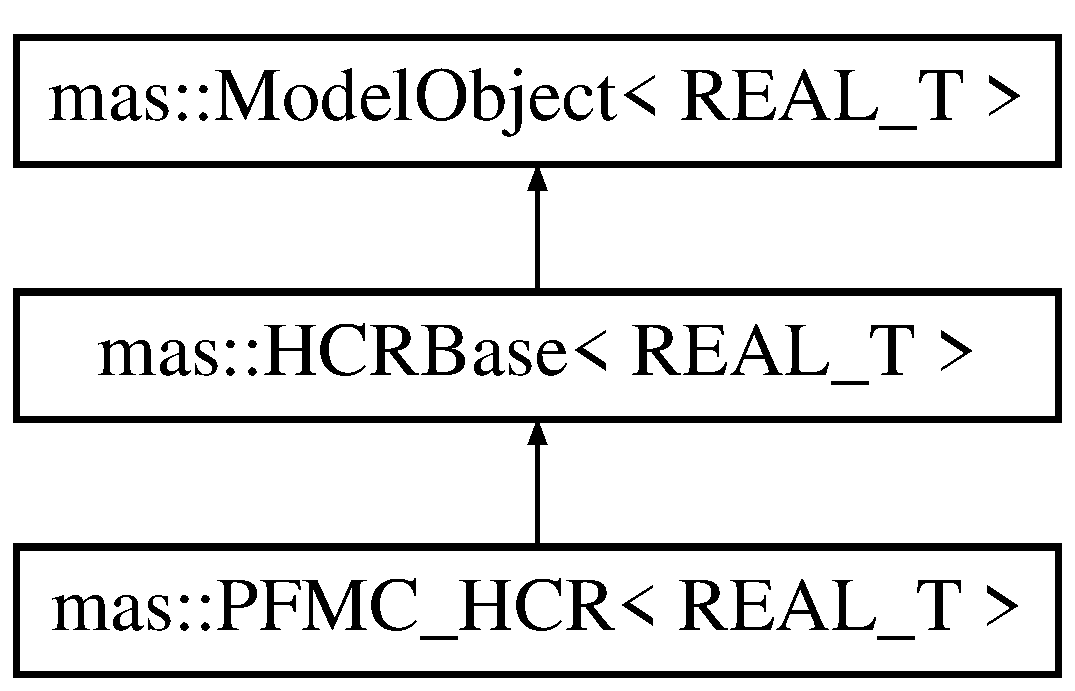
\includegraphics[height=3.000000cm]{structmas_1_1_p_f_m_c___h_c_r}
\end{center}
\end{figure}
\subsection*{Public Types}
\begin{DoxyCompactItemize}
\item 
typedef \hyperlink{structmas_1_1_variable_trait}{Variable\-Trait}$<$ R\-E\-A\-L\-\_\-\-T $>$\\*
\-::\hyperlink{structmas_1_1_p_f_m_c___h_c_r_a1fd22811f88e2214903cfbf887f68aaf}{variable} \hyperlink{structmas_1_1_p_f_m_c___h_c_r_a1fd22811f88e2214903cfbf887f68aaf}{variable}
\end{DoxyCompactItemize}
\subsection*{Public Member Functions}
\begin{DoxyCompactItemize}
\item 
const std\-::tuple$<$ \hyperlink{structmas_1_1_p_f_m_c___h_c_r_a1fd22811f88e2214903cfbf887f68aaf}{variable}, \\*
\hyperlink{structmas_1_1_p_f_m_c___h_c_r_a1fd22811f88e2214903cfbf887f68aaf}{variable}, \hyperlink{structmas_1_1_p_f_m_c___h_c_r_a1fd22811f88e2214903cfbf887f68aaf}{variable}, \hyperlink{structmas_1_1_p_f_m_c___h_c_r_a1fd22811f88e2214903cfbf887f68aaf}{variable} $>$ \hyperlink{structmas_1_1_p_f_m_c___h_c_r_a8e71e3c20bd5404dd350b9aca573a294}{Evaluate} (const int \&year, const \hyperlink{structmas_1_1_area_population_info}{mas\-::\-Area\-Population\-Info}$<$ R\-E\-A\-L\-\_\-\-T $>$ \&api\-\_\-males, const \hyperlink{structmas_1_1_area_population_info}{mas\-::\-Area\-Population\-Info}$<$ R\-E\-A\-L\-\_\-\-T $>$ \&api\-\_\-females)
\item 
const std\-::string \hyperlink{structmas_1_1_p_f_m_c___h_c_r_a5571d69b3043c8a56b92e96a4f1837b5}{Name} ()
\end{DoxyCompactItemize}
\subsection*{Public Attributes}
\begin{DoxyCompactItemize}
\item 
\hyperlink{structmas_1_1_p_f_m_c___h_c_r_a1fd22811f88e2214903cfbf887f68aaf}{variable} \hyperlink{structmas_1_1_p_f_m_c___h_c_r_a9ef690cc5957f768d4ac4924bde499df}{F\-\_\-\-A\-B\-C}
\item 
\hyperlink{structmas_1_1_p_f_m_c___h_c_r_a1fd22811f88e2214903cfbf887f68aaf}{variable} \hyperlink{structmas_1_1_p_f_m_c___h_c_r_aeb488a01a83c2ad95756e8904ce5d76b}{A\-B\-C}
\item 
\hyperlink{structmas_1_1_p_f_m_c___h_c_r_a1fd22811f88e2214903cfbf887f68aaf}{variable} \hyperlink{structmas_1_1_p_f_m_c___h_c_r_a5804d2123da3f0ec617ad3f559920c9f}{F\-\_\-\-O\-F\-L}
\item 
\hyperlink{structmas_1_1_p_f_m_c___h_c_r_a1fd22811f88e2214903cfbf887f68aaf}{variable} \hyperlink{structmas_1_1_p_f_m_c___h_c_r_a5f4d1fefb9913ab7baa38590c80efa83}{O\-F\-L}
\end{DoxyCompactItemize}


\subsection{Detailed Description}
\subsubsection*{template$<$typename R\-E\-A\-L\-\_\-\-T$>$struct mas\-::\-P\-F\-M\-C\-\_\-\-H\-C\-R$<$ R\-E\-A\-L\-\_\-\-T $>$}



Definition at line 290 of file Harvest\-Control\-Rule.\-hpp.



\subsection{Member Typedef Documentation}
\hypertarget{structmas_1_1_p_f_m_c___h_c_r_a1fd22811f88e2214903cfbf887f68aaf}{\index{mas\-::\-P\-F\-M\-C\-\_\-\-H\-C\-R@{mas\-::\-P\-F\-M\-C\-\_\-\-H\-C\-R}!variable@{variable}}
\index{variable@{variable}!mas::PFMC_HCR@{mas\-::\-P\-F\-M\-C\-\_\-\-H\-C\-R}}
\subsubsection[{variable}]{\setlength{\rightskip}{0pt plus 5cm}template$<$typename R\-E\-A\-L\-\_\-\-T $>$ typedef {\bf Variable\-Trait}$<$R\-E\-A\-L\-\_\-\-T$>$\-::{\bf variable} {\bf mas\-::\-P\-F\-M\-C\-\_\-\-H\-C\-R}$<$ R\-E\-A\-L\-\_\-\-T $>$\-::{\bf variable}}}\label{structmas_1_1_p_f_m_c___h_c_r_a1fd22811f88e2214903cfbf887f68aaf}


Definition at line 292 of file Harvest\-Control\-Rule.\-hpp.



\subsection{Member Function Documentation}
\hypertarget{structmas_1_1_p_f_m_c___h_c_r_a8e71e3c20bd5404dd350b9aca573a294}{\index{mas\-::\-P\-F\-M\-C\-\_\-\-H\-C\-R@{mas\-::\-P\-F\-M\-C\-\_\-\-H\-C\-R}!Evaluate@{Evaluate}}
\index{Evaluate@{Evaluate}!mas::PFMC_HCR@{mas\-::\-P\-F\-M\-C\-\_\-\-H\-C\-R}}
\subsubsection[{Evaluate}]{\setlength{\rightskip}{0pt plus 5cm}template$<$typename R\-E\-A\-L\-\_\-\-T $>$ const std\-::tuple$<${\bf variable}, {\bf variable}, {\bf variable}, {\bf variable}$>$ {\bf mas\-::\-P\-F\-M\-C\-\_\-\-H\-C\-R}$<$ R\-E\-A\-L\-\_\-\-T $>$\-::Evaluate (
\begin{DoxyParamCaption}
\item[{const int \&}]{year, }
\item[{const {\bf mas\-::\-Area\-Population\-Info}$<$ R\-E\-A\-L\-\_\-\-T $>$ \&}]{api\-\_\-males, }
\item[{const {\bf mas\-::\-Area\-Population\-Info}$<$ R\-E\-A\-L\-\_\-\-T $>$ \&}]{api\-\_\-females}
\end{DoxyParamCaption}
)\hspace{0.3cm}{\ttfamily [inline]}, {\ttfamily [virtual]}}}\label{structmas_1_1_p_f_m_c___h_c_r_a8e71e3c20bd5404dd350b9aca573a294}


Implements \hyperlink{structmas_1_1_h_c_r_base_a3d923b3276f10e4c7938abde6a134291}{mas\-::\-H\-C\-R\-Base$<$ R\-E\-A\-L\-\_\-\-T $>$}.



Definition at line 296 of file Harvest\-Control\-Rule.\-hpp.

\hypertarget{structmas_1_1_p_f_m_c___h_c_r_a5571d69b3043c8a56b92e96a4f1837b5}{\index{mas\-::\-P\-F\-M\-C\-\_\-\-H\-C\-R@{mas\-::\-P\-F\-M\-C\-\_\-\-H\-C\-R}!Name@{Name}}
\index{Name@{Name}!mas::PFMC_HCR@{mas\-::\-P\-F\-M\-C\-\_\-\-H\-C\-R}}
\subsubsection[{Name}]{\setlength{\rightskip}{0pt plus 5cm}template$<$typename R\-E\-A\-L\-\_\-\-T $>$ const std\-::string {\bf mas\-::\-P\-F\-M\-C\-\_\-\-H\-C\-R}$<$ R\-E\-A\-L\-\_\-\-T $>$\-::Name (
\begin{DoxyParamCaption}
{}
\end{DoxyParamCaption}
)\hspace{0.3cm}{\ttfamily [inline]}, {\ttfamily [virtual]}}}\label{structmas_1_1_p_f_m_c___h_c_r_a5571d69b3043c8a56b92e96a4f1837b5}


Reimplemented from \hyperlink{structmas_1_1_h_c_r_base_a3f1aa4335bee8d9225776ca5212e1085}{mas\-::\-H\-C\-R\-Base$<$ R\-E\-A\-L\-\_\-\-T $>$}.



Definition at line 307 of file Harvest\-Control\-Rule.\-hpp.



\subsection{Member Data Documentation}
\hypertarget{structmas_1_1_p_f_m_c___h_c_r_aeb488a01a83c2ad95756e8904ce5d76b}{\index{mas\-::\-P\-F\-M\-C\-\_\-\-H\-C\-R@{mas\-::\-P\-F\-M\-C\-\_\-\-H\-C\-R}!A\-B\-C@{A\-B\-C}}
\index{A\-B\-C@{A\-B\-C}!mas::PFMC_HCR@{mas\-::\-P\-F\-M\-C\-\_\-\-H\-C\-R}}
\subsubsection[{A\-B\-C}]{\setlength{\rightskip}{0pt plus 5cm}template$<$typename R\-E\-A\-L\-\_\-\-T $>$ {\bf variable} {\bf mas\-::\-P\-F\-M\-C\-\_\-\-H\-C\-R}$<$ R\-E\-A\-L\-\_\-\-T $>$\-::A\-B\-C}}\label{structmas_1_1_p_f_m_c___h_c_r_aeb488a01a83c2ad95756e8904ce5d76b}


Definition at line 294 of file Harvest\-Control\-Rule.\-hpp.

\hypertarget{structmas_1_1_p_f_m_c___h_c_r_a9ef690cc5957f768d4ac4924bde499df}{\index{mas\-::\-P\-F\-M\-C\-\_\-\-H\-C\-R@{mas\-::\-P\-F\-M\-C\-\_\-\-H\-C\-R}!F\-\_\-\-A\-B\-C@{F\-\_\-\-A\-B\-C}}
\index{F\-\_\-\-A\-B\-C@{F\-\_\-\-A\-B\-C}!mas::PFMC_HCR@{mas\-::\-P\-F\-M\-C\-\_\-\-H\-C\-R}}
\subsubsection[{F\-\_\-\-A\-B\-C}]{\setlength{\rightskip}{0pt plus 5cm}template$<$typename R\-E\-A\-L\-\_\-\-T $>$ {\bf variable} {\bf mas\-::\-P\-F\-M\-C\-\_\-\-H\-C\-R}$<$ R\-E\-A\-L\-\_\-\-T $>$\-::F\-\_\-\-A\-B\-C}}\label{structmas_1_1_p_f_m_c___h_c_r_a9ef690cc5957f768d4ac4924bde499df}


Definition at line 294 of file Harvest\-Control\-Rule.\-hpp.

\hypertarget{structmas_1_1_p_f_m_c___h_c_r_a5804d2123da3f0ec617ad3f559920c9f}{\index{mas\-::\-P\-F\-M\-C\-\_\-\-H\-C\-R@{mas\-::\-P\-F\-M\-C\-\_\-\-H\-C\-R}!F\-\_\-\-O\-F\-L@{F\-\_\-\-O\-F\-L}}
\index{F\-\_\-\-O\-F\-L@{F\-\_\-\-O\-F\-L}!mas::PFMC_HCR@{mas\-::\-P\-F\-M\-C\-\_\-\-H\-C\-R}}
\subsubsection[{F\-\_\-\-O\-F\-L}]{\setlength{\rightskip}{0pt plus 5cm}template$<$typename R\-E\-A\-L\-\_\-\-T $>$ {\bf variable} {\bf mas\-::\-P\-F\-M\-C\-\_\-\-H\-C\-R}$<$ R\-E\-A\-L\-\_\-\-T $>$\-::F\-\_\-\-O\-F\-L}}\label{structmas_1_1_p_f_m_c___h_c_r_a5804d2123da3f0ec617ad3f559920c9f}


Definition at line 294 of file Harvest\-Control\-Rule.\-hpp.

\hypertarget{structmas_1_1_p_f_m_c___h_c_r_a5f4d1fefb9913ab7baa38590c80efa83}{\index{mas\-::\-P\-F\-M\-C\-\_\-\-H\-C\-R@{mas\-::\-P\-F\-M\-C\-\_\-\-H\-C\-R}!O\-F\-L@{O\-F\-L}}
\index{O\-F\-L@{O\-F\-L}!mas::PFMC_HCR@{mas\-::\-P\-F\-M\-C\-\_\-\-H\-C\-R}}
\subsubsection[{O\-F\-L}]{\setlength{\rightskip}{0pt plus 5cm}template$<$typename R\-E\-A\-L\-\_\-\-T $>$ {\bf variable} {\bf mas\-::\-P\-F\-M\-C\-\_\-\-H\-C\-R}$<$ R\-E\-A\-L\-\_\-\-T $>$\-::O\-F\-L}}\label{structmas_1_1_p_f_m_c___h_c_r_a5f4d1fefb9913ab7baa38590c80efa83}


Definition at line 294 of file Harvest\-Control\-Rule.\-hpp.



The documentation for this struct was generated from the following file\-:\begin{DoxyCompactItemize}
\item 
/home/oppy/\-Net\-Beans\-Projects/mas/\hyperlink{_harvest_control_rule_8hpp}{Harvest\-Control\-Rule.\-hpp}\end{DoxyCompactItemize}

\hypertarget{classmas_1_1_population}{\section{mas\-:\-:Population$<$ R\-E\-A\-L\-\_\-\-T $>$ Class Template Reference}
\label{classmas_1_1_population}\index{mas\-::\-Population$<$ R\-E\-A\-L\-\_\-\-T $>$@{mas\-::\-Population$<$ R\-E\-A\-L\-\_\-\-T $>$}}
}


{\ttfamily \#include $<$Population.\-hpp$>$}

Inheritance diagram for mas\-:\-:Population$<$ R\-E\-A\-L\-\_\-\-T $>$\-:\begin{figure}[H]
\begin{center}
\leavevmode
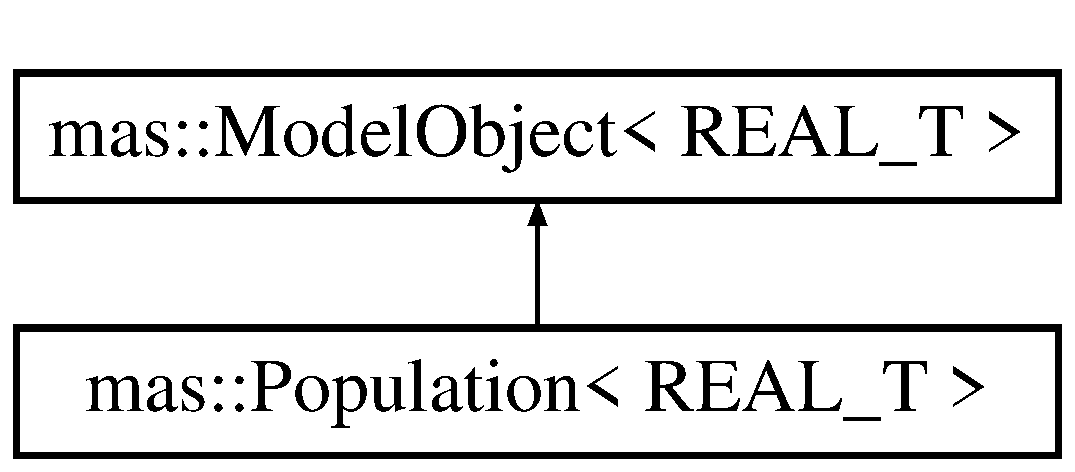
\includegraphics[height=2.000000cm]{classmas_1_1_population}
\end{center}
\end{figure}
\subsection*{Public Types}
\begin{DoxyCompactItemize}
\item 
typedef std\-::map$<$ int, int $>$\\*
\-::iterator \hyperlink{classmas_1_1_population_aed3c87441d95effcc96071a1ac6ad69c}{male\-\_\-natural\-\_\-mortality\-\_\-ids\-\_\-iterator}
\item 
typedef std\-::map$<$ int, int $>$\\*
\-::iterator \hyperlink{classmas_1_1_population_a96fc8c402905ebb808d78ae6c61953c9}{female\-\_\-natural\-\_\-mortality\-\_\-ids\-\_\-iterator}
\item 
typedef std\-::unordered\-\_\-map\\*
$<$ int, std\-::unordered\-\_\-map$<$ int, \\*
int $>$ $>$\-::iterator \hyperlink{classmas_1_1_population_ab971002bd0166bba55d86c73fd92d46a}{season\-\_\-area\-\_\-id\-\_\-iterator}
\item 
typedef std\-::map$<$ int, int $>$\\*
\-::iterator \hyperlink{classmas_1_1_population_a0aaaac61b68d5d8aa0e385067e05283c}{recruitment\-\_\-ids\-\_\-iterator}
\item 
typedef \hyperlink{structmas_1_1_variable_trait}{mas\-::\-Variable\-Trait}\\*
$<$ R\-E\-A\-L\-\_\-\-T $>$\-::\hyperlink{classmas_1_1_population_a55b9219455246e0cab7f84ae49f0271f}{variable} \hyperlink{classmas_1_1_population_a55b9219455246e0cab7f84ae49f0271f}{variable}
\item 
typedef std\-::unordered\-\_\-map\\*
$<$ int, \hyperlink{structmas_1_1_area_population_info}{Area\-Population\-Info}\\*
$<$ R\-E\-A\-L\-\_\-\-T $>$ $>$\-::iterator \hyperlink{classmas_1_1_population_a82c4fbea27716a8e9e64a34cf867ad43}{cohort\-\_\-iterator}
\item 
typedef std\-::unordered\-\_\-map\\*
$<$ int, int $>$\-::iterator \hyperlink{classmas_1_1_population_a60d48584943ae2846d15045f7696aafb}{movement\-\_\-model\-\_\-id\-\_\-iterator}
\item 
typedef std\-::unordered\-\_\-map\\*
$<$ int, std\-::shared\-\_\-ptr\\*
$<$ \hyperlink{structmas_1_1_movement}{mas\-::\-Movement}$<$ R\-E\-A\-L\-\_\-\-T $>$\\*
 $>$ $>$\-::iterator \hyperlink{classmas_1_1_population_a7c0c3438d8b5c223cb3ca7072d5e84bc}{movement\-\_\-model\-\_\-iterator}
\item 
typedef std\-::unordered\-\_\-map\\*
$<$ int, std\-::unordered\-\_\-map$<$ int, \\*
std\-::vector$<$ R\-E\-A\-L\-\_\-\-T $>$\\*
 $>$ $>$\-::iterator \hyperlink{classmas_1_1_population_ac63fa975ca5b6070604a82240a0d297b}{maturity\-\_\-models\-\_\-iterator}
\item 
typedef std\-::unordered\-\_\-map\\*
$<$ int, std\-::vector$<$ R\-E\-A\-L\-\_\-\-T $>$\\*
 $>$\-::iterator \hyperlink{classmas_1_1_population_a6c5591e255cb99b132de23c5c2a6dbaa}{area\-\_\-maturity\-\_\-model\-\_\-iterator}
\end{DoxyCompactItemize}
\subsection*{Public Member Functions}
\begin{DoxyCompactItemize}
\item 
\hyperlink{classmas_1_1_population_a34502c0d5d6e7a40be3cc1990ba77f30}{Population} ()
\item 
\hyperlink{classmas_1_1_population_ab816687c71192f6c9e4399021ffb9527}{Population} (int \hyperlink{classmas_1_1_population_a3c5b11c403479bdc518727551791ed21}{years}, int \hyperlink{classmas_1_1_population_a3ff65a37b33f558530ed8fa065d79eb6}{seasons}, int \hyperlink{classmas_1_1_population_a5dbc73c77f78382e1d7dadfa1b24dfb8}{areas}, const std\-::shared\-\_\-ptr$<$ \hyperlink{structmas_1_1_area}{Area}$<$ R\-E\-A\-L\-\_\-\-T $>$ $>$ \&\hyperlink{classmas_1_1_population_a5ce5f6317dd632ccbf1961d0b0eca4d6}{natal\-\_\-area}, const std\-::vector$<$ std\-::shared\-\_\-ptr$<$ \hyperlink{structmas_1_1_area}{Area}$<$ R\-E\-A\-L\-\_\-\-T $>$ $>$ $>$ \&\hyperlink{classmas_1_1_population_a3633009c9043c6531989337ab8749ab3}{areas\-\_\-list})
\item 
void \hyperlink{classmas_1_1_population_a1d36dfded5ba625dd54dad0281fe201e}{Prepare} ()
\item 
void \hyperlink{classmas_1_1_population_aa109008ecb4e00a72e5c3eda31108c35}{Increment\-Time} (int \&y, int \&s)
\item 
void \hyperlink{classmas_1_1_population_a8b5d6f0d26543e164d1f86d46dccfdf2}{Decrement\-Time} (int \&y, int \&s)
\item 
void \hyperlink{classmas_1_1_population_ae0908df961a197feee21286c5b7d322a}{Move\-Fish} (int year, int season)
\item 
void \hyperlink{classmas_1_1_population_a5e6afe8e961d769cd95dfbee49c904d4}{Initialize\-Populationin\-Areas} ()
\item 
void \hyperlink{classmas_1_1_population_af4a03fed8e5d6654a91a582b5898b39f}{Initialize} ()
\item 
void \hyperlink{classmas_1_1_population_a8ff4779365c94ab8fb92f71f26d0e516}{Show} ()
\item 
virtual const std\-::string \hyperlink{classmas_1_1_population_a772b5663ac871067411c7227ed66094a}{Name} ()
\item 
virtual const std\-::string \hyperlink{classmas_1_1_population_adb6e6afabb8a27f64592f36909d43612}{To\-J\-S\-O\-N\-String} ()
\item 
void \hyperlink{classmas_1_1_population_a86400790b65e5bd774782e8919312a5f}{Evaluate} ()
\item 
void \hyperlink{classmas_1_1_population_a37a20f21ea890ff806d96122bebdbec4}{Push\-To\-Areas\-And\-Fleets} ()
\end{DoxyCompactItemize}
\subsection*{Public Attributes}
\begin{DoxyCompactItemize}
\item 
int \hyperlink{classmas_1_1_population_ac1239c7b55a78c996eceb83c8c399a0b}{phase} = 1
\item 
int \hyperlink{classmas_1_1_population_a69ed32e9b8a91451da22927333ed7b76}{previous\-\_\-phase} = 1
\item 
std\-::map$<$ int, int $>$ \hyperlink{classmas_1_1_population_a5448f2e0761a208a5184f754b3efbbc6}{male\-\_\-natural\-\_\-mortality\-\_\-ids}
\item 
std\-::map$<$ int, int $>$ \hyperlink{classmas_1_1_population_a87a2beba70c06531b7fcfab50f0ab76d}{female\-\_\-natural\-\_\-mortality\-\_\-ids}
\item 
std\-::unordered\-\_\-map$<$ int, \\*
std\-::unordered\-\_\-map$<$ int, int $>$ $>$ \hyperlink{classmas_1_1_population_a06d567e1aee12655a0442ff6e79464b7}{area\-\_\-season\-\_\-recruitment\-\_\-ids}
\item 
std\-::unordered\-\_\-map$<$ int, \\*
std\-::unordered\-\_\-map$<$ int, \\*
std\-::shared\-\_\-ptr\\*
$<$ \hyperlink{structmas_1_1_recruitment_base}{mas\-::\-Recruitment\-Base}$<$ R\-E\-A\-L\-\_\-\-T $>$ $>$ $>$ $>$ \hyperlink{classmas_1_1_population_ae6b75bd5f2b821e43b3b256255f1b8d6}{area\-\_\-season\-\_\-recruitment}
\item 
std\-::unordered\-\_\-map$<$ int, \\*
std\-::unordered\-\_\-map$<$ int, int $>$ $>$ \hyperlink{classmas_1_1_population_ada1429ef3172d164cffc39fce103454b}{season\-\_\-area\-\_\-recruitment\-\_\-ids}
\item 
std\-::unordered\-\_\-map$<$ int, \\*
std\-::unordered\-\_\-map$<$ int, \\*
std\-::shared\-\_\-ptr\\*
$<$ \hyperlink{structmas_1_1_recruitment_base}{mas\-::\-Recruitment\-Base}$<$ R\-E\-A\-L\-\_\-\-T $>$ $>$ $>$ $>$ \hyperlink{classmas_1_1_population_a4447806c7275aaf07e7d205c94754405}{season\-\_\-area\-\_\-recruitment}
\item 
std\-::map$<$ int, int $>$ \hyperlink{classmas_1_1_population_a37e238439828debf37c7d69b952c52d4}{recruitment\-\_\-ids}
\item 
std\-::string \hyperlink{classmas_1_1_population_a44500e45226461f286df00fc98b354cb}{name}
\item 
int \hyperlink{classmas_1_1_population_a035dfbc2bc4a4c379cd1ea272d58d103}{natal\-\_\-area\-\_\-id}
\item 
int \hyperlink{classmas_1_1_population_a445c1fbf6d76206a93b243f7e39b8279}{movement\-\_\-model\-\_\-id}
\item 
bool \hyperlink{classmas_1_1_population_a851c5669637dc6d7333b9f5124a7f867}{natal\-\_\-homing} = false
\item 
bool \hyperlink{classmas_1_1_population_add42454aa09f82776039538f7b87a2c9}{natal\-\_\-recruitment} = false
\item 
bool \hyperlink{classmas_1_1_population_a94c79dddb366eb6702f4a2cfd77c3eb8}{move\-\_\-fish\-\_\-before\-\_\-lh} = false
\item 
int \hyperlink{classmas_1_1_population_a3c5b11c403479bdc518727551791ed21}{years}
\item 
int \hyperlink{classmas_1_1_population_a3ff65a37b33f558530ed8fa065d79eb6}{seasons}
\item 
int \hyperlink{classmas_1_1_population_a5dbc73c77f78382e1d7dadfa1b24dfb8}{areas}
\item 
int \hyperlink{classmas_1_1_population_a0012e4e055a3a2c661097ae30a4c18e7}{ages}
\item 
int \hyperlink{classmas_1_1_population_a2720b3c93f0fc25a600dd37becebd3d7}{growth\-\_\-id}
\item 
std\-::vector$<$ \hyperlink{classmas_1_1_population_a55b9219455246e0cab7f84ae49f0271f}{variable} $>$ \hyperlink{classmas_1_1_population_ad305739a2b90cd6947b4f847a0de46eb}{S\-N}
\item 
std\-::vector$<$ \hyperlink{classmas_1_1_population_a55b9219455246e0cab7f84ae49f0271f}{variable} $>$ \hyperlink{classmas_1_1_population_ad41f0a54ab4be79a144b1b61a5fe7436}{S\-N\-\_\-\-Biomass}
\item 
std\-::vector$<$ \hyperlink{classmas_1_1_population_a55b9219455246e0cab7f84ae49f0271f}{variable} $>$ \hyperlink{classmas_1_1_population_a878a062c7c1cb82ad02c0f42417c072c}{C}
\item 
std\-::vector$<$ \hyperlink{classmas_1_1_population_a55b9219455246e0cab7f84ae49f0271f}{variable} $>$ \hyperlink{classmas_1_1_population_ad3554c8cd3320e57770a1f793359c62f}{C\-\_\-\-Biomass}
\item 
std\-::shared\-\_\-ptr$<$ \hyperlink{structmas_1_1_area}{Area}$<$ R\-E\-A\-L\-\_\-\-T $>$ $>$ \hyperlink{classmas_1_1_population_a5ce5f6317dd632ccbf1961d0b0eca4d6}{natal\-\_\-area}
\item 
std\-::vector$<$ std\-::shared\-\_\-ptr\\*
$<$ \hyperlink{structmas_1_1_area}{Area}$<$ R\-E\-A\-L\-\_\-\-T $>$ $>$ $>$ \hyperlink{classmas_1_1_population_a3633009c9043c6531989337ab8749ab3}{areas\-\_\-list}
\item 
std\-::unordered\-\_\-map$<$ int, \\*
\hyperlink{structmas_1_1_area_population_info}{Area\-Population\-Info}$<$ R\-E\-A\-L\-\_\-\-T $>$ $>$ \hyperlink{classmas_1_1_population_a224336670db7b89a7d9490fddbbf88f1}{males}
\item 
std\-::unordered\-\_\-map$<$ int, \\*
\hyperlink{structmas_1_1_area_population_info}{Area\-Population\-Info}$<$ R\-E\-A\-L\-\_\-\-T $>$ $>$ \hyperlink{classmas_1_1_population_adeeb5c8b2056ea2bc21d7d57ec700ae5}{females}
\item 
std\-::unordered\-\_\-map$<$ int, int $>$ \hyperlink{classmas_1_1_population_ab98ba8e32dbc1650b3452adaa6bd09e1}{movement\-\_\-models\-\_\-ids}
\item 
std\-::shared\-\_\-ptr$<$ \hyperlink{structmas_1_1_movement}{mas\-::\-Movement}\\*
$<$ R\-E\-A\-L\-\_\-\-T $>$ $>$ \hyperlink{classmas_1_1_population_a8452be41c1534e55f5c8169655f8f6c3}{movement\-\_\-model}
\item 
std\-::unordered\-\_\-map$<$ int, \\*
std\-::shared\-\_\-ptr$<$ \hyperlink{structmas_1_1_movement}{mas\-::\-Movement}\\*
$<$ R\-E\-A\-L\-\_\-\-T $>$ $>$ $>$ \hyperlink{classmas_1_1_population_ae53093b412fcb3c074a90fccdfc747fe}{movement\-\_\-models}
\item 
std\-::vector$<$ std\-::vector\\*
$<$ \hyperlink{classmas_1_1_population_a55b9219455246e0cab7f84ae49f0271f}{variable} $>$ $>$ \hyperlink{classmas_1_1_population_a99d5b7c5e089b8313abaffe5491848bc}{movement\-\_\-coefficients}
\item 
std\-::unordered\-\_\-map$<$ int, \\*
std\-::unordered\-\_\-map$<$ int, \\*
std\-::vector$<$ R\-E\-A\-L\-\_\-\-T $>$ $>$ $>$ \hyperlink{classmas_1_1_population_a4953be176d66e895dafa26d3754339a7}{maturity\-\_\-models}
\item 
std\-::shared\-\_\-ptr$<$ \hyperlink{structmas_1_1_h_c_r_base}{mas\-::\-H\-C\-R\-Base}\\*
$<$ R\-E\-A\-L\-\_\-\-T $>$ $>$ \hyperlink{classmas_1_1_population_a161064be0d713a6a0481f297f84f5729}{harvest\-\_\-control\-\_\-rule}
\item 
std\-::unordered\-\_\-set$<$ int $>$ \hyperlink{classmas_1_1_population_a4d87c6a8ce6a0ad5b65f5209a103094c}{active\-\_\-fleets}
\end{DoxyCompactItemize}


\subsection{Detailed Description}
\subsubsection*{template$<$class R\-E\-A\-L\-\_\-\-T$>$class mas\-::\-Population$<$ R\-E\-A\-L\-\_\-\-T $>$}



Definition at line 36 of file Population.\-hpp.



\subsection{Member Typedef Documentation}
\hypertarget{classmas_1_1_population_a6c5591e255cb99b132de23c5c2a6dbaa}{\index{mas\-::\-Population@{mas\-::\-Population}!area\-\_\-maturity\-\_\-model\-\_\-iterator@{area\-\_\-maturity\-\_\-model\-\_\-iterator}}
\index{area\-\_\-maturity\-\_\-model\-\_\-iterator@{area\-\_\-maturity\-\_\-model\-\_\-iterator}!mas::Population@{mas\-::\-Population}}
\subsubsection[{area\-\_\-maturity\-\_\-model\-\_\-iterator}]{\setlength{\rightskip}{0pt plus 5cm}template$<$class R\-E\-A\-L\-\_\-\-T$>$ typedef std\-::unordered\-\_\-map$<$int, std\-::vector$<$R\-E\-A\-L\-\_\-\-T$>$ $>$\-::iterator {\bf mas\-::\-Population}$<$ R\-E\-A\-L\-\_\-\-T $>$\-::{\bf area\-\_\-maturity\-\_\-model\-\_\-iterator}}}\label{classmas_1_1_population_a6c5591e255cb99b132de23c5c2a6dbaa}


Definition at line 1449 of file Population.\-hpp.

\hypertarget{classmas_1_1_population_a82c4fbea27716a8e9e64a34cf867ad43}{\index{mas\-::\-Population@{mas\-::\-Population}!cohort\-\_\-iterator@{cohort\-\_\-iterator}}
\index{cohort\-\_\-iterator@{cohort\-\_\-iterator}!mas::Population@{mas\-::\-Population}}
\subsubsection[{cohort\-\_\-iterator}]{\setlength{\rightskip}{0pt plus 5cm}template$<$class R\-E\-A\-L\-\_\-\-T$>$ typedef std\-::unordered\-\_\-map$<$int, {\bf Area\-Population\-Info}$<$R\-E\-A\-L\-\_\-\-T$>$ $>$\-::iterator {\bf mas\-::\-Population}$<$ R\-E\-A\-L\-\_\-\-T $>$\-::{\bf cohort\-\_\-iterator}}}\label{classmas_1_1_population_a82c4fbea27716a8e9e64a34cf867ad43}


Definition at line 1433 of file Population.\-hpp.

\hypertarget{classmas_1_1_population_a96fc8c402905ebb808d78ae6c61953c9}{\index{mas\-::\-Population@{mas\-::\-Population}!female\-\_\-natural\-\_\-mortality\-\_\-ids\-\_\-iterator@{female\-\_\-natural\-\_\-mortality\-\_\-ids\-\_\-iterator}}
\index{female\-\_\-natural\-\_\-mortality\-\_\-ids\-\_\-iterator@{female\-\_\-natural\-\_\-mortality\-\_\-ids\-\_\-iterator}!mas::Population@{mas\-::\-Population}}
\subsubsection[{female\-\_\-natural\-\_\-mortality\-\_\-ids\-\_\-iterator}]{\setlength{\rightskip}{0pt plus 5cm}template$<$class R\-E\-A\-L\-\_\-\-T$>$ typedef std\-::map$<$int, int$>$\-::iterator {\bf mas\-::\-Population}$<$ R\-E\-A\-L\-\_\-\-T $>$\-::{\bf female\-\_\-natural\-\_\-mortality\-\_\-ids\-\_\-iterator}}}\label{classmas_1_1_population_a96fc8c402905ebb808d78ae6c61953c9}


Definition at line 1393 of file Population.\-hpp.

\hypertarget{classmas_1_1_population_aed3c87441d95effcc96071a1ac6ad69c}{\index{mas\-::\-Population@{mas\-::\-Population}!male\-\_\-natural\-\_\-mortality\-\_\-ids\-\_\-iterator@{male\-\_\-natural\-\_\-mortality\-\_\-ids\-\_\-iterator}}
\index{male\-\_\-natural\-\_\-mortality\-\_\-ids\-\_\-iterator@{male\-\_\-natural\-\_\-mortality\-\_\-ids\-\_\-iterator}!mas::Population@{mas\-::\-Population}}
\subsubsection[{male\-\_\-natural\-\_\-mortality\-\_\-ids\-\_\-iterator}]{\setlength{\rightskip}{0pt plus 5cm}template$<$class R\-E\-A\-L\-\_\-\-T$>$ typedef std\-::map$<$int, int$>$\-::iterator {\bf mas\-::\-Population}$<$ R\-E\-A\-L\-\_\-\-T $>$\-::{\bf male\-\_\-natural\-\_\-mortality\-\_\-ids\-\_\-iterator}}}\label{classmas_1_1_population_aed3c87441d95effcc96071a1ac6ad69c}


Definition at line 1392 of file Population.\-hpp.

\hypertarget{classmas_1_1_population_ac63fa975ca5b6070604a82240a0d297b}{\index{mas\-::\-Population@{mas\-::\-Population}!maturity\-\_\-models\-\_\-iterator@{maturity\-\_\-models\-\_\-iterator}}
\index{maturity\-\_\-models\-\_\-iterator@{maturity\-\_\-models\-\_\-iterator}!mas::Population@{mas\-::\-Population}}
\subsubsection[{maturity\-\_\-models\-\_\-iterator}]{\setlength{\rightskip}{0pt plus 5cm}template$<$class R\-E\-A\-L\-\_\-\-T$>$ typedef std\-::unordered\-\_\-map$<$int, std\-::unordered\-\_\-map$<$int, std\-::vector$<$R\-E\-A\-L\-\_\-\-T$>$ $>$ $>$\-::iterator {\bf mas\-::\-Population}$<$ R\-E\-A\-L\-\_\-\-T $>$\-::{\bf maturity\-\_\-models\-\_\-iterator}}}\label{classmas_1_1_population_ac63fa975ca5b6070604a82240a0d297b}


Definition at line 1448 of file Population.\-hpp.

\hypertarget{classmas_1_1_population_a60d48584943ae2846d15045f7696aafb}{\index{mas\-::\-Population@{mas\-::\-Population}!movement\-\_\-model\-\_\-id\-\_\-iterator@{movement\-\_\-model\-\_\-id\-\_\-iterator}}
\index{movement\-\_\-model\-\_\-id\-\_\-iterator@{movement\-\_\-model\-\_\-id\-\_\-iterator}!mas::Population@{mas\-::\-Population}}
\subsubsection[{movement\-\_\-model\-\_\-id\-\_\-iterator}]{\setlength{\rightskip}{0pt plus 5cm}template$<$class R\-E\-A\-L\-\_\-\-T$>$ typedef std\-::unordered\-\_\-map$<$int, int $>$\-::iterator {\bf mas\-::\-Population}$<$ R\-E\-A\-L\-\_\-\-T $>$\-::{\bf movement\-\_\-model\-\_\-id\-\_\-iterator}}}\label{classmas_1_1_population_a60d48584943ae2846d15045f7696aafb}


Definition at line 1437 of file Population.\-hpp.

\hypertarget{classmas_1_1_population_a7c0c3438d8b5c223cb3ca7072d5e84bc}{\index{mas\-::\-Population@{mas\-::\-Population}!movement\-\_\-model\-\_\-iterator@{movement\-\_\-model\-\_\-iterator}}
\index{movement\-\_\-model\-\_\-iterator@{movement\-\_\-model\-\_\-iterator}!mas::Population@{mas\-::\-Population}}
\subsubsection[{movement\-\_\-model\-\_\-iterator}]{\setlength{\rightskip}{0pt plus 5cm}template$<$class R\-E\-A\-L\-\_\-\-T$>$ typedef std\-::unordered\-\_\-map$<$int, std\-::shared\-\_\-ptr$<${\bf mas\-::\-Movement}$<$R\-E\-A\-L\-\_\-\-T$>$ $>$ $>$\-::iterator {\bf mas\-::\-Population}$<$ R\-E\-A\-L\-\_\-\-T $>$\-::{\bf movement\-\_\-model\-\_\-iterator}}}\label{classmas_1_1_population_a7c0c3438d8b5c223cb3ca7072d5e84bc}


Definition at line 1442 of file Population.\-hpp.

\hypertarget{classmas_1_1_population_a0aaaac61b68d5d8aa0e385067e05283c}{\index{mas\-::\-Population@{mas\-::\-Population}!recruitment\-\_\-ids\-\_\-iterator@{recruitment\-\_\-ids\-\_\-iterator}}
\index{recruitment\-\_\-ids\-\_\-iterator@{recruitment\-\_\-ids\-\_\-iterator}!mas::Population@{mas\-::\-Population}}
\subsubsection[{recruitment\-\_\-ids\-\_\-iterator}]{\setlength{\rightskip}{0pt plus 5cm}template$<$class R\-E\-A\-L\-\_\-\-T$>$ typedef std\-::map$<$int, int$>$\-::iterator {\bf mas\-::\-Population}$<$ R\-E\-A\-L\-\_\-\-T $>$\-::{\bf recruitment\-\_\-ids\-\_\-iterator}}}\label{classmas_1_1_population_a0aaaac61b68d5d8aa0e385067e05283c}


Definition at line 1407 of file Population.\-hpp.

\hypertarget{classmas_1_1_population_ab971002bd0166bba55d86c73fd92d46a}{\index{mas\-::\-Population@{mas\-::\-Population}!season\-\_\-area\-\_\-id\-\_\-iterator@{season\-\_\-area\-\_\-id\-\_\-iterator}}
\index{season\-\_\-area\-\_\-id\-\_\-iterator@{season\-\_\-area\-\_\-id\-\_\-iterator}!mas::Population@{mas\-::\-Population}}
\subsubsection[{season\-\_\-area\-\_\-id\-\_\-iterator}]{\setlength{\rightskip}{0pt plus 5cm}template$<$class R\-E\-A\-L\-\_\-\-T$>$ typedef std\-::unordered\-\_\-map$<$int, std\-::unordered\-\_\-map$<$int, int$>$ $>$\-::iterator {\bf mas\-::\-Population}$<$ R\-E\-A\-L\-\_\-\-T $>$\-::{\bf season\-\_\-area\-\_\-id\-\_\-iterator}}}\label{classmas_1_1_population_ab971002bd0166bba55d86c73fd92d46a}


Definition at line 1400 of file Population.\-hpp.

\hypertarget{classmas_1_1_population_a55b9219455246e0cab7f84ae49f0271f}{\index{mas\-::\-Population@{mas\-::\-Population}!variable@{variable}}
\index{variable@{variable}!mas::Population@{mas\-::\-Population}}
\subsubsection[{variable}]{\setlength{\rightskip}{0pt plus 5cm}template$<$class R\-E\-A\-L\-\_\-\-T$>$ typedef {\bf mas\-::\-Variable\-Trait}$<$R\-E\-A\-L\-\_\-\-T$>$\-::{\bf variable} {\bf mas\-::\-Population}$<$ R\-E\-A\-L\-\_\-\-T $>$\-::{\bf variable}}}\label{classmas_1_1_population_a55b9219455246e0cab7f84ae49f0271f}


Definition at line 1410 of file Population.\-hpp.



\subsection{Constructor \& Destructor Documentation}
\hypertarget{classmas_1_1_population_a34502c0d5d6e7a40be3cc1990ba77f30}{\index{mas\-::\-Population@{mas\-::\-Population}!Population@{Population}}
\index{Population@{Population}!mas::Population@{mas\-::\-Population}}
\subsubsection[{Population}]{\setlength{\rightskip}{0pt plus 5cm}template$<$class R\-E\-A\-L\-\_\-\-T$>$ {\bf mas\-::\-Population}$<$ R\-E\-A\-L\-\_\-\-T $>$\-::{\bf Population} (
\begin{DoxyParamCaption}
{}
\end{DoxyParamCaption}
)\hspace{0.3cm}{\ttfamily [inline]}}}\label{classmas_1_1_population_a34502c0d5d6e7a40be3cc1990ba77f30}


Definition at line 1458 of file Population.\-hpp.

\hypertarget{classmas_1_1_population_ab816687c71192f6c9e4399021ffb9527}{\index{mas\-::\-Population@{mas\-::\-Population}!Population@{Population}}
\index{Population@{Population}!mas::Population@{mas\-::\-Population}}
\subsubsection[{Population}]{\setlength{\rightskip}{0pt plus 5cm}template$<$class R\-E\-A\-L\-\_\-\-T$>$ {\bf mas\-::\-Population}$<$ R\-E\-A\-L\-\_\-\-T $>$\-::{\bf Population} (
\begin{DoxyParamCaption}
\item[{int}]{years, }
\item[{int}]{seasons, }
\item[{int}]{areas, }
\item[{const std\-::shared\-\_\-ptr$<$ {\bf Area}$<$ R\-E\-A\-L\-\_\-\-T $>$ $>$ \&}]{natal\-\_\-area, }
\item[{const std\-::vector$<$ std\-::shared\-\_\-ptr$<$ {\bf Area}$<$ R\-E\-A\-L\-\_\-\-T $>$ $>$ $>$ \&}]{areas\-\_\-list}
\end{DoxyParamCaption}
)\hspace{0.3cm}{\ttfamily [inline]}}}\label{classmas_1_1_population_ab816687c71192f6c9e4399021ffb9527}


Definition at line 1461 of file Population.\-hpp.



\subsection{Member Function Documentation}
\hypertarget{classmas_1_1_population_a8b5d6f0d26543e164d1f86d46dccfdf2}{\index{mas\-::\-Population@{mas\-::\-Population}!Decrement\-Time@{Decrement\-Time}}
\index{Decrement\-Time@{Decrement\-Time}!mas::Population@{mas\-::\-Population}}
\subsubsection[{Decrement\-Time}]{\setlength{\rightskip}{0pt plus 5cm}template$<$class R\-E\-A\-L\-\_\-\-T$>$ void {\bf mas\-::\-Population}$<$ R\-E\-A\-L\-\_\-\-T $>$\-::Decrement\-Time (
\begin{DoxyParamCaption}
\item[{int \&}]{y, }
\item[{int \&}]{s}
\end{DoxyParamCaption}
)\hspace{0.3cm}{\ttfamily [inline]}}}\label{classmas_1_1_population_a8b5d6f0d26543e164d1f86d46dccfdf2}


Definition at line 1514 of file Population.\-hpp.

\hypertarget{classmas_1_1_population_a86400790b65e5bd774782e8919312a5f}{\index{mas\-::\-Population@{mas\-::\-Population}!Evaluate@{Evaluate}}
\index{Evaluate@{Evaluate}!mas::Population@{mas\-::\-Population}}
\subsubsection[{Evaluate}]{\setlength{\rightskip}{0pt plus 5cm}template$<$class R\-E\-A\-L\-\_\-\-T$>$ void {\bf mas\-::\-Population}$<$ R\-E\-A\-L\-\_\-\-T $>$\-::Evaluate (
\begin{DoxyParamCaption}
{}
\end{DoxyParamCaption}
)\hspace{0.3cm}{\ttfamily [inline]}}}\label{classmas_1_1_population_a86400790b65e5bd774782e8919312a5f}
Compute totals for this population

Definition at line 1847 of file Population.\-hpp.

\hypertarget{classmas_1_1_population_aa109008ecb4e00a72e5c3eda31108c35}{\index{mas\-::\-Population@{mas\-::\-Population}!Increment\-Time@{Increment\-Time}}
\index{Increment\-Time@{Increment\-Time}!mas::Population@{mas\-::\-Population}}
\subsubsection[{Increment\-Time}]{\setlength{\rightskip}{0pt plus 5cm}template$<$class R\-E\-A\-L\-\_\-\-T$>$ void {\bf mas\-::\-Population}$<$ R\-E\-A\-L\-\_\-\-T $>$\-::Increment\-Time (
\begin{DoxyParamCaption}
\item[{int \&}]{y, }
\item[{int \&}]{s}
\end{DoxyParamCaption}
)\hspace{0.3cm}{\ttfamily [inline]}}}\label{classmas_1_1_population_aa109008ecb4e00a72e5c3eda31108c35}


Definition at line 1505 of file Population.\-hpp.

\hypertarget{classmas_1_1_population_af4a03fed8e5d6654a91a582b5898b39f}{\index{mas\-::\-Population@{mas\-::\-Population}!Initialize@{Initialize}}
\index{Initialize@{Initialize}!mas::Population@{mas\-::\-Population}}
\subsubsection[{Initialize}]{\setlength{\rightskip}{0pt plus 5cm}template$<$class R\-E\-A\-L\-\_\-\-T$>$ void {\bf mas\-::\-Population}$<$ R\-E\-A\-L\-\_\-\-T $>$\-::Initialize (
\begin{DoxyParamCaption}
{}
\end{DoxyParamCaption}
)\hspace{0.3cm}{\ttfamily [inline]}}}\label{classmas_1_1_population_af4a03fed8e5d6654a91a582b5898b39f}


Definition at line 1610 of file Population.\-hpp.

\hypertarget{classmas_1_1_population_a5e6afe8e961d769cd95dfbee49c904d4}{\index{mas\-::\-Population@{mas\-::\-Population}!Initialize\-Populationin\-Areas@{Initialize\-Populationin\-Areas}}
\index{Initialize\-Populationin\-Areas@{Initialize\-Populationin\-Areas}!mas::Population@{mas\-::\-Population}}
\subsubsection[{Initialize\-Populationin\-Areas}]{\setlength{\rightskip}{0pt plus 5cm}template$<$class R\-E\-A\-L\-\_\-\-T$>$ void {\bf mas\-::\-Population}$<$ R\-E\-A\-L\-\_\-\-T $>$\-::Initialize\-Populationin\-Areas (
\begin{DoxyParamCaption}
{}
\end{DoxyParamCaption}
)\hspace{0.3cm}{\ttfamily [inline]}}}\label{classmas_1_1_population_a5e6afe8e961d769cd95dfbee49c904d4}


Definition at line 1586 of file Population.\-hpp.

\hypertarget{classmas_1_1_population_ae0908df961a197feee21286c5b7d322a}{\index{mas\-::\-Population@{mas\-::\-Population}!Move\-Fish@{Move\-Fish}}
\index{Move\-Fish@{Move\-Fish}!mas::Population@{mas\-::\-Population}}
\subsubsection[{Move\-Fish}]{\setlength{\rightskip}{0pt plus 5cm}template$<$class R\-E\-A\-L\-\_\-\-T$>$ void {\bf mas\-::\-Population}$<$ R\-E\-A\-L\-\_\-\-T $>$\-::Move\-Fish (
\begin{DoxyParamCaption}
\item[{int}]{year, }
\item[{int}]{season}
\end{DoxyParamCaption}
)\hspace{0.3cm}{\ttfamily [inline]}}}\label{classmas_1_1_population_ae0908df961a197feee21286c5b7d322a}


Definition at line 1523 of file Population.\-hpp.

\hypertarget{classmas_1_1_population_a772b5663ac871067411c7227ed66094a}{\index{mas\-::\-Population@{mas\-::\-Population}!Name@{Name}}
\index{Name@{Name}!mas::Population@{mas\-::\-Population}}
\subsubsection[{Name}]{\setlength{\rightskip}{0pt plus 5cm}template$<$class R\-E\-A\-L\-\_\-\-T$>$ virtual const std\-::string {\bf mas\-::\-Population}$<$ R\-E\-A\-L\-\_\-\-T $>$\-::Name (
\begin{DoxyParamCaption}
{}
\end{DoxyParamCaption}
)\hspace{0.3cm}{\ttfamily [inline]}, {\ttfamily [virtual]}}}\label{classmas_1_1_population_a772b5663ac871067411c7227ed66094a}


Definition at line 1727 of file Population.\-hpp.

\hypertarget{classmas_1_1_population_a1d36dfded5ba625dd54dad0281fe201e}{\index{mas\-::\-Population@{mas\-::\-Population}!Prepare@{Prepare}}
\index{Prepare@{Prepare}!mas::Population@{mas\-::\-Population}}
\subsubsection[{Prepare}]{\setlength{\rightskip}{0pt plus 5cm}template$<$class R\-E\-A\-L\-\_\-\-T$>$ void {\bf mas\-::\-Population}$<$ R\-E\-A\-L\-\_\-\-T $>$\-::Prepare (
\begin{DoxyParamCaption}
{}
\end{DoxyParamCaption}
)\hspace{0.3cm}{\ttfamily [inline]}}}\label{classmas_1_1_population_a1d36dfded5ba625dd54dad0281fe201e}


Definition at line 1487 of file Population.\-hpp.

\hypertarget{classmas_1_1_population_a37a20f21ea890ff806d96122bebdbec4}{\index{mas\-::\-Population@{mas\-::\-Population}!Push\-To\-Areas\-And\-Fleets@{Push\-To\-Areas\-And\-Fleets}}
\index{Push\-To\-Areas\-And\-Fleets@{Push\-To\-Areas\-And\-Fleets}!mas::Population@{mas\-::\-Population}}
\subsubsection[{Push\-To\-Areas\-And\-Fleets}]{\setlength{\rightskip}{0pt plus 5cm}template$<$class R\-E\-A\-L\-\_\-\-T$>$ void {\bf mas\-::\-Population}$<$ R\-E\-A\-L\-\_\-\-T $>$\-::Push\-To\-Areas\-And\-Fleets (
\begin{DoxyParamCaption}
{}
\end{DoxyParamCaption}
)\hspace{0.3cm}{\ttfamily [inline]}}}\label{classmas_1_1_population_a37a20f21ea890ff806d96122bebdbec4}


Definition at line 1932 of file Population.\-hpp.

\hypertarget{classmas_1_1_population_a8ff4779365c94ab8fb92f71f26d0e516}{\index{mas\-::\-Population@{mas\-::\-Population}!Show@{Show}}
\index{Show@{Show}!mas::Population@{mas\-::\-Population}}
\subsubsection[{Show}]{\setlength{\rightskip}{0pt plus 5cm}template$<$class R\-E\-A\-L\-\_\-\-T$>$ void {\bf mas\-::\-Population}$<$ R\-E\-A\-L\-\_\-\-T $>$\-::Show (
\begin{DoxyParamCaption}
{}
\end{DoxyParamCaption}
)\hspace{0.3cm}{\ttfamily [inline]}}}\label{classmas_1_1_population_a8ff4779365c94ab8fb92f71f26d0e516}


Definition at line 1663 of file Population.\-hpp.

\hypertarget{classmas_1_1_population_adb6e6afabb8a27f64592f36909d43612}{\index{mas\-::\-Population@{mas\-::\-Population}!To\-J\-S\-O\-N\-String@{To\-J\-S\-O\-N\-String}}
\index{To\-J\-S\-O\-N\-String@{To\-J\-S\-O\-N\-String}!mas::Population@{mas\-::\-Population}}
\subsubsection[{To\-J\-S\-O\-N\-String}]{\setlength{\rightskip}{0pt plus 5cm}template$<$class R\-E\-A\-L\-\_\-\-T$>$ virtual const std\-::string {\bf mas\-::\-Population}$<$ R\-E\-A\-L\-\_\-\-T $>$\-::To\-J\-S\-O\-N\-String (
\begin{DoxyParamCaption}
{}
\end{DoxyParamCaption}
)\hspace{0.3cm}{\ttfamily [inline]}, {\ttfamily [virtual]}}}\label{classmas_1_1_population_adb6e6afabb8a27f64592f36909d43612}


Reimplemented from \hyperlink{structmas_1_1_model_object_af40b3c89b11919fc5aea21dcf1cd027b}{mas\-::\-Model\-Object$<$ R\-E\-A\-L\-\_\-\-T $>$}.



Definition at line 1731 of file Population.\-hpp.



\subsection{Member Data Documentation}
\hypertarget{classmas_1_1_population_a4d87c6a8ce6a0ad5b65f5209a103094c}{\index{mas\-::\-Population@{mas\-::\-Population}!active\-\_\-fleets@{active\-\_\-fleets}}
\index{active\-\_\-fleets@{active\-\_\-fleets}!mas::Population@{mas\-::\-Population}}
\subsubsection[{active\-\_\-fleets}]{\setlength{\rightskip}{0pt plus 5cm}template$<$class R\-E\-A\-L\-\_\-\-T$>$ std\-::unordered\-\_\-set$<$int$>$ {\bf mas\-::\-Population}$<$ R\-E\-A\-L\-\_\-\-T $>$\-::active\-\_\-fleets}}\label{classmas_1_1_population_a4d87c6a8ce6a0ad5b65f5209a103094c}


Definition at line 1456 of file Population.\-hpp.

\hypertarget{classmas_1_1_population_a0012e4e055a3a2c661097ae30a4c18e7}{\index{mas\-::\-Population@{mas\-::\-Population}!ages@{ages}}
\index{ages@{ages}!mas::Population@{mas\-::\-Population}}
\subsubsection[{ages}]{\setlength{\rightskip}{0pt plus 5cm}template$<$class R\-E\-A\-L\-\_\-\-T$>$ int {\bf mas\-::\-Population}$<$ R\-E\-A\-L\-\_\-\-T $>$\-::ages}}\label{classmas_1_1_population_a0012e4e055a3a2c661097ae30a4c18e7}


Definition at line 1421 of file Population.\-hpp.

\hypertarget{classmas_1_1_population_ae6b75bd5f2b821e43b3b256255f1b8d6}{\index{mas\-::\-Population@{mas\-::\-Population}!area\-\_\-season\-\_\-recruitment@{area\-\_\-season\-\_\-recruitment}}
\index{area\-\_\-season\-\_\-recruitment@{area\-\_\-season\-\_\-recruitment}!mas::Population@{mas\-::\-Population}}
\subsubsection[{area\-\_\-season\-\_\-recruitment}]{\setlength{\rightskip}{0pt plus 5cm}template$<$class R\-E\-A\-L\-\_\-\-T$>$ std\-::unordered\-\_\-map$<$int, std\-::unordered\-\_\-map$<$int, std\-::shared\-\_\-ptr$<${\bf mas\-::\-Recruitment\-Base}$<$R\-E\-A\-L\-\_\-\-T$>$ $>$ $>$ $>$ {\bf mas\-::\-Population}$<$ R\-E\-A\-L\-\_\-\-T $>$\-::area\-\_\-season\-\_\-recruitment}}\label{classmas_1_1_population_ae6b75bd5f2b821e43b3b256255f1b8d6}


Definition at line 1401 of file Population.\-hpp.

\hypertarget{classmas_1_1_population_a06d567e1aee12655a0442ff6e79464b7}{\index{mas\-::\-Population@{mas\-::\-Population}!area\-\_\-season\-\_\-recruitment\-\_\-ids@{area\-\_\-season\-\_\-recruitment\-\_\-ids}}
\index{area\-\_\-season\-\_\-recruitment\-\_\-ids@{area\-\_\-season\-\_\-recruitment\-\_\-ids}!mas::Population@{mas\-::\-Population}}
\subsubsection[{area\-\_\-season\-\_\-recruitment\-\_\-ids}]{\setlength{\rightskip}{0pt plus 5cm}template$<$class R\-E\-A\-L\-\_\-\-T$>$ std\-::unordered\-\_\-map$<$int, std\-::unordered\-\_\-map$<$int, int$>$ $>$ {\bf mas\-::\-Population}$<$ R\-E\-A\-L\-\_\-\-T $>$\-::area\-\_\-season\-\_\-recruitment\-\_\-ids}}\label{classmas_1_1_population_a06d567e1aee12655a0442ff6e79464b7}


Definition at line 1399 of file Population.\-hpp.

\hypertarget{classmas_1_1_population_a5dbc73c77f78382e1d7dadfa1b24dfb8}{\index{mas\-::\-Population@{mas\-::\-Population}!areas@{areas}}
\index{areas@{areas}!mas::Population@{mas\-::\-Population}}
\subsubsection[{areas}]{\setlength{\rightskip}{0pt plus 5cm}template$<$class R\-E\-A\-L\-\_\-\-T$>$ int {\bf mas\-::\-Population}$<$ R\-E\-A\-L\-\_\-\-T $>$\-::areas}}\label{classmas_1_1_population_a5dbc73c77f78382e1d7dadfa1b24dfb8}


Definition at line 1420 of file Population.\-hpp.

\hypertarget{classmas_1_1_population_a3633009c9043c6531989337ab8749ab3}{\index{mas\-::\-Population@{mas\-::\-Population}!areas\-\_\-list@{areas\-\_\-list}}
\index{areas\-\_\-list@{areas\-\_\-list}!mas::Population@{mas\-::\-Population}}
\subsubsection[{areas\-\_\-list}]{\setlength{\rightskip}{0pt plus 5cm}template$<$class R\-E\-A\-L\-\_\-\-T$>$ std\-::vector$<$std\-::shared\-\_\-ptr$<${\bf Area}$<$R\-E\-A\-L\-\_\-\-T$>$ $>$ $>$ {\bf mas\-::\-Population}$<$ R\-E\-A\-L\-\_\-\-T $>$\-::areas\-\_\-list}}\label{classmas_1_1_population_a3633009c9043c6531989337ab8749ab3}


Definition at line 1430 of file Population.\-hpp.

\hypertarget{classmas_1_1_population_a878a062c7c1cb82ad02c0f42417c072c}{\index{mas\-::\-Population@{mas\-::\-Population}!C@{C}}
\index{C@{C}!mas::Population@{mas\-::\-Population}}
\subsubsection[{C}]{\setlength{\rightskip}{0pt plus 5cm}template$<$class R\-E\-A\-L\-\_\-\-T$>$ std\-::vector$<${\bf variable}$>$ {\bf mas\-::\-Population}$<$ R\-E\-A\-L\-\_\-\-T $>$\-::C}}\label{classmas_1_1_population_a878a062c7c1cb82ad02c0f42417c072c}


Definition at line 1426 of file Population.\-hpp.

\hypertarget{classmas_1_1_population_ad3554c8cd3320e57770a1f793359c62f}{\index{mas\-::\-Population@{mas\-::\-Population}!C\-\_\-\-Biomass@{C\-\_\-\-Biomass}}
\index{C\-\_\-\-Biomass@{C\-\_\-\-Biomass}!mas::Population@{mas\-::\-Population}}
\subsubsection[{C\-\_\-\-Biomass}]{\setlength{\rightskip}{0pt plus 5cm}template$<$class R\-E\-A\-L\-\_\-\-T$>$ std\-::vector$<${\bf variable}$>$ {\bf mas\-::\-Population}$<$ R\-E\-A\-L\-\_\-\-T $>$\-::C\-\_\-\-Biomass}}\label{classmas_1_1_population_ad3554c8cd3320e57770a1f793359c62f}


Definition at line 1427 of file Population.\-hpp.

\hypertarget{classmas_1_1_population_a87a2beba70c06531b7fcfab50f0ab76d}{\index{mas\-::\-Population@{mas\-::\-Population}!female\-\_\-natural\-\_\-mortality\-\_\-ids@{female\-\_\-natural\-\_\-mortality\-\_\-ids}}
\index{female\-\_\-natural\-\_\-mortality\-\_\-ids@{female\-\_\-natural\-\_\-mortality\-\_\-ids}!mas::Population@{mas\-::\-Population}}
\subsubsection[{female\-\_\-natural\-\_\-mortality\-\_\-ids}]{\setlength{\rightskip}{0pt plus 5cm}template$<$class R\-E\-A\-L\-\_\-\-T$>$ std\-::map$<$int, int$>$ {\bf mas\-::\-Population}$<$ R\-E\-A\-L\-\_\-\-T $>$\-::female\-\_\-natural\-\_\-mortality\-\_\-ids}}\label{classmas_1_1_population_a87a2beba70c06531b7fcfab50f0ab76d}


Definition at line 1391 of file Population.\-hpp.

\hypertarget{classmas_1_1_population_adeeb5c8b2056ea2bc21d7d57ec700ae5}{\index{mas\-::\-Population@{mas\-::\-Population}!females@{females}}
\index{females@{females}!mas::Population@{mas\-::\-Population}}
\subsubsection[{females}]{\setlength{\rightskip}{0pt plus 5cm}template$<$class R\-E\-A\-L\-\_\-\-T$>$ std\-::unordered\-\_\-map$<$int, {\bf Area\-Population\-Info}$<$R\-E\-A\-L\-\_\-\-T$>$ $>$ {\bf mas\-::\-Population}$<$ R\-E\-A\-L\-\_\-\-T $>$\-::females}}\label{classmas_1_1_population_adeeb5c8b2056ea2bc21d7d57ec700ae5}


Definition at line 1435 of file Population.\-hpp.

\hypertarget{classmas_1_1_population_a2720b3c93f0fc25a600dd37becebd3d7}{\index{mas\-::\-Population@{mas\-::\-Population}!growth\-\_\-id@{growth\-\_\-id}}
\index{growth\-\_\-id@{growth\-\_\-id}!mas::Population@{mas\-::\-Population}}
\subsubsection[{growth\-\_\-id}]{\setlength{\rightskip}{0pt plus 5cm}template$<$class R\-E\-A\-L\-\_\-\-T$>$ int {\bf mas\-::\-Population}$<$ R\-E\-A\-L\-\_\-\-T $>$\-::growth\-\_\-id}}\label{classmas_1_1_population_a2720b3c93f0fc25a600dd37becebd3d7}


Definition at line 1422 of file Population.\-hpp.

\hypertarget{classmas_1_1_population_a161064be0d713a6a0481f297f84f5729}{\index{mas\-::\-Population@{mas\-::\-Population}!harvest\-\_\-control\-\_\-rule@{harvest\-\_\-control\-\_\-rule}}
\index{harvest\-\_\-control\-\_\-rule@{harvest\-\_\-control\-\_\-rule}!mas::Population@{mas\-::\-Population}}
\subsubsection[{harvest\-\_\-control\-\_\-rule}]{\setlength{\rightskip}{0pt plus 5cm}template$<$class R\-E\-A\-L\-\_\-\-T$>$ std\-::shared\-\_\-ptr$<${\bf mas\-::\-H\-C\-R\-Base}$<$R\-E\-A\-L\-\_\-\-T$>$ $>$ {\bf mas\-::\-Population}$<$ R\-E\-A\-L\-\_\-\-T $>$\-::harvest\-\_\-control\-\_\-rule}}\label{classmas_1_1_population_a161064be0d713a6a0481f297f84f5729}


Definition at line 1454 of file Population.\-hpp.

\hypertarget{classmas_1_1_population_a5448f2e0761a208a5184f754b3efbbc6}{\index{mas\-::\-Population@{mas\-::\-Population}!male\-\_\-natural\-\_\-mortality\-\_\-ids@{male\-\_\-natural\-\_\-mortality\-\_\-ids}}
\index{male\-\_\-natural\-\_\-mortality\-\_\-ids@{male\-\_\-natural\-\_\-mortality\-\_\-ids}!mas::Population@{mas\-::\-Population}}
\subsubsection[{male\-\_\-natural\-\_\-mortality\-\_\-ids}]{\setlength{\rightskip}{0pt plus 5cm}template$<$class R\-E\-A\-L\-\_\-\-T$>$ std\-::map$<$int, int$>$ {\bf mas\-::\-Population}$<$ R\-E\-A\-L\-\_\-\-T $>$\-::male\-\_\-natural\-\_\-mortality\-\_\-ids}}\label{classmas_1_1_population_a5448f2e0761a208a5184f754b3efbbc6}


Definition at line 1390 of file Population.\-hpp.

\hypertarget{classmas_1_1_population_a224336670db7b89a7d9490fddbbf88f1}{\index{mas\-::\-Population@{mas\-::\-Population}!males@{males}}
\index{males@{males}!mas::Population@{mas\-::\-Population}}
\subsubsection[{males}]{\setlength{\rightskip}{0pt plus 5cm}template$<$class R\-E\-A\-L\-\_\-\-T$>$ std\-::unordered\-\_\-map$<$int, {\bf Area\-Population\-Info}$<$R\-E\-A\-L\-\_\-\-T$>$ $>$ {\bf mas\-::\-Population}$<$ R\-E\-A\-L\-\_\-\-T $>$\-::males}}\label{classmas_1_1_population_a224336670db7b89a7d9490fddbbf88f1}


Definition at line 1434 of file Population.\-hpp.

\hypertarget{classmas_1_1_population_a4953be176d66e895dafa26d3754339a7}{\index{mas\-::\-Population@{mas\-::\-Population}!maturity\-\_\-models@{maturity\-\_\-models}}
\index{maturity\-\_\-models@{maturity\-\_\-models}!mas::Population@{mas\-::\-Population}}
\subsubsection[{maturity\-\_\-models}]{\setlength{\rightskip}{0pt plus 5cm}template$<$class R\-E\-A\-L\-\_\-\-T$>$ std\-::unordered\-\_\-map$<$int, std\-::unordered\-\_\-map$<$int, std\-::vector$<$R\-E\-A\-L\-\_\-\-T$>$ $>$ $>$ {\bf mas\-::\-Population}$<$ R\-E\-A\-L\-\_\-\-T $>$\-::maturity\-\_\-models}}\label{classmas_1_1_population_a4953be176d66e895dafa26d3754339a7}


Definition at line 1447 of file Population.\-hpp.

\hypertarget{classmas_1_1_population_a94c79dddb366eb6702f4a2cfd77c3eb8}{\index{mas\-::\-Population@{mas\-::\-Population}!move\-\_\-fish\-\_\-before\-\_\-lh@{move\-\_\-fish\-\_\-before\-\_\-lh}}
\index{move\-\_\-fish\-\_\-before\-\_\-lh@{move\-\_\-fish\-\_\-before\-\_\-lh}!mas::Population@{mas\-::\-Population}}
\subsubsection[{move\-\_\-fish\-\_\-before\-\_\-lh}]{\setlength{\rightskip}{0pt plus 5cm}template$<$class R\-E\-A\-L\-\_\-\-T$>$ bool {\bf mas\-::\-Population}$<$ R\-E\-A\-L\-\_\-\-T $>$\-::move\-\_\-fish\-\_\-before\-\_\-lh = false}}\label{classmas_1_1_population_a94c79dddb366eb6702f4a2cfd77c3eb8}


Definition at line 1416 of file Population.\-hpp.

\hypertarget{classmas_1_1_population_a99d5b7c5e089b8313abaffe5491848bc}{\index{mas\-::\-Population@{mas\-::\-Population}!movement\-\_\-coefficients@{movement\-\_\-coefficients}}
\index{movement\-\_\-coefficients@{movement\-\_\-coefficients}!mas::Population@{mas\-::\-Population}}
\subsubsection[{movement\-\_\-coefficients}]{\setlength{\rightskip}{0pt plus 5cm}template$<$class R\-E\-A\-L\-\_\-\-T$>$ std\-::vector$<$std\-::vector$<${\bf variable}$>$ $>$ {\bf mas\-::\-Population}$<$ R\-E\-A\-L\-\_\-\-T $>$\-::movement\-\_\-coefficients}}\label{classmas_1_1_population_a99d5b7c5e089b8313abaffe5491848bc}


Definition at line 1444 of file Population.\-hpp.

\hypertarget{classmas_1_1_population_a8452be41c1534e55f5c8169655f8f6c3}{\index{mas\-::\-Population@{mas\-::\-Population}!movement\-\_\-model@{movement\-\_\-model}}
\index{movement\-\_\-model@{movement\-\_\-model}!mas::Population@{mas\-::\-Population}}
\subsubsection[{movement\-\_\-model}]{\setlength{\rightskip}{0pt plus 5cm}template$<$class R\-E\-A\-L\-\_\-\-T$>$ std\-::shared\-\_\-ptr$<${\bf mas\-::\-Movement}$<$R\-E\-A\-L\-\_\-\-T$>$ $>$ {\bf mas\-::\-Population}$<$ R\-E\-A\-L\-\_\-\-T $>$\-::movement\-\_\-model}}\label{classmas_1_1_population_a8452be41c1534e55f5c8169655f8f6c3}


Definition at line 1439 of file Population.\-hpp.

\hypertarget{classmas_1_1_population_a445c1fbf6d76206a93b243f7e39b8279}{\index{mas\-::\-Population@{mas\-::\-Population}!movement\-\_\-model\-\_\-id@{movement\-\_\-model\-\_\-id}}
\index{movement\-\_\-model\-\_\-id@{movement\-\_\-model\-\_\-id}!mas::Population@{mas\-::\-Population}}
\subsubsection[{movement\-\_\-model\-\_\-id}]{\setlength{\rightskip}{0pt plus 5cm}template$<$class R\-E\-A\-L\-\_\-\-T$>$ int {\bf mas\-::\-Population}$<$ R\-E\-A\-L\-\_\-\-T $>$\-::movement\-\_\-model\-\_\-id}}\label{classmas_1_1_population_a445c1fbf6d76206a93b243f7e39b8279}


Definition at line 1413 of file Population.\-hpp.

\hypertarget{classmas_1_1_population_ae53093b412fcb3c074a90fccdfc747fe}{\index{mas\-::\-Population@{mas\-::\-Population}!movement\-\_\-models@{movement\-\_\-models}}
\index{movement\-\_\-models@{movement\-\_\-models}!mas::Population@{mas\-::\-Population}}
\subsubsection[{movement\-\_\-models}]{\setlength{\rightskip}{0pt plus 5cm}template$<$class R\-E\-A\-L\-\_\-\-T$>$ std\-::unordered\-\_\-map$<$int, std\-::shared\-\_\-ptr$<${\bf mas\-::\-Movement}$<$R\-E\-A\-L\-\_\-\-T$>$ $>$ $>$ {\bf mas\-::\-Population}$<$ R\-E\-A\-L\-\_\-\-T $>$\-::movement\-\_\-models}}\label{classmas_1_1_population_ae53093b412fcb3c074a90fccdfc747fe}


Definition at line 1441 of file Population.\-hpp.

\hypertarget{classmas_1_1_population_ab98ba8e32dbc1650b3452adaa6bd09e1}{\index{mas\-::\-Population@{mas\-::\-Population}!movement\-\_\-models\-\_\-ids@{movement\-\_\-models\-\_\-ids}}
\index{movement\-\_\-models\-\_\-ids@{movement\-\_\-models\-\_\-ids}!mas::Population@{mas\-::\-Population}}
\subsubsection[{movement\-\_\-models\-\_\-ids}]{\setlength{\rightskip}{0pt plus 5cm}template$<$class R\-E\-A\-L\-\_\-\-T$>$ std\-::unordered\-\_\-map$<$int, int $>$ {\bf mas\-::\-Population}$<$ R\-E\-A\-L\-\_\-\-T $>$\-::movement\-\_\-models\-\_\-ids}}\label{classmas_1_1_population_ab98ba8e32dbc1650b3452adaa6bd09e1}


Definition at line 1436 of file Population.\-hpp.

\hypertarget{classmas_1_1_population_a44500e45226461f286df00fc98b354cb}{\index{mas\-::\-Population@{mas\-::\-Population}!name@{name}}
\index{name@{name}!mas::Population@{mas\-::\-Population}}
\subsubsection[{name}]{\setlength{\rightskip}{0pt plus 5cm}template$<$class R\-E\-A\-L\-\_\-\-T$>$ std\-::string {\bf mas\-::\-Population}$<$ R\-E\-A\-L\-\_\-\-T $>$\-::name}}\label{classmas_1_1_population_a44500e45226461f286df00fc98b354cb}


Definition at line 1411 of file Population.\-hpp.

\hypertarget{classmas_1_1_population_a5ce5f6317dd632ccbf1961d0b0eca4d6}{\index{mas\-::\-Population@{mas\-::\-Population}!natal\-\_\-area@{natal\-\_\-area}}
\index{natal\-\_\-area@{natal\-\_\-area}!mas::Population@{mas\-::\-Population}}
\subsubsection[{natal\-\_\-area}]{\setlength{\rightskip}{0pt plus 5cm}template$<$class R\-E\-A\-L\-\_\-\-T$>$ std\-::shared\-\_\-ptr$<${\bf Area}$<$R\-E\-A\-L\-\_\-\-T$>$ $>$ {\bf mas\-::\-Population}$<$ R\-E\-A\-L\-\_\-\-T $>$\-::natal\-\_\-area}}\label{classmas_1_1_population_a5ce5f6317dd632ccbf1961d0b0eca4d6}


Definition at line 1429 of file Population.\-hpp.

\hypertarget{classmas_1_1_population_a035dfbc2bc4a4c379cd1ea272d58d103}{\index{mas\-::\-Population@{mas\-::\-Population}!natal\-\_\-area\-\_\-id@{natal\-\_\-area\-\_\-id}}
\index{natal\-\_\-area\-\_\-id@{natal\-\_\-area\-\_\-id}!mas::Population@{mas\-::\-Population}}
\subsubsection[{natal\-\_\-area\-\_\-id}]{\setlength{\rightskip}{0pt plus 5cm}template$<$class R\-E\-A\-L\-\_\-\-T$>$ int {\bf mas\-::\-Population}$<$ R\-E\-A\-L\-\_\-\-T $>$\-::natal\-\_\-area\-\_\-id}}\label{classmas_1_1_population_a035dfbc2bc4a4c379cd1ea272d58d103}


Definition at line 1412 of file Population.\-hpp.

\hypertarget{classmas_1_1_population_a851c5669637dc6d7333b9f5124a7f867}{\index{mas\-::\-Population@{mas\-::\-Population}!natal\-\_\-homing@{natal\-\_\-homing}}
\index{natal\-\_\-homing@{natal\-\_\-homing}!mas::Population@{mas\-::\-Population}}
\subsubsection[{natal\-\_\-homing}]{\setlength{\rightskip}{0pt plus 5cm}template$<$class R\-E\-A\-L\-\_\-\-T$>$ bool {\bf mas\-::\-Population}$<$ R\-E\-A\-L\-\_\-\-T $>$\-::natal\-\_\-homing = false}}\label{classmas_1_1_population_a851c5669637dc6d7333b9f5124a7f867}


Definition at line 1414 of file Population.\-hpp.

\hypertarget{classmas_1_1_population_add42454aa09f82776039538f7b87a2c9}{\index{mas\-::\-Population@{mas\-::\-Population}!natal\-\_\-recruitment@{natal\-\_\-recruitment}}
\index{natal\-\_\-recruitment@{natal\-\_\-recruitment}!mas::Population@{mas\-::\-Population}}
\subsubsection[{natal\-\_\-recruitment}]{\setlength{\rightskip}{0pt plus 5cm}template$<$class R\-E\-A\-L\-\_\-\-T$>$ bool {\bf mas\-::\-Population}$<$ R\-E\-A\-L\-\_\-\-T $>$\-::natal\-\_\-recruitment = false}}\label{classmas_1_1_population_add42454aa09f82776039538f7b87a2c9}


Definition at line 1415 of file Population.\-hpp.

\hypertarget{classmas_1_1_population_ac1239c7b55a78c996eceb83c8c399a0b}{\index{mas\-::\-Population@{mas\-::\-Population}!phase@{phase}}
\index{phase@{phase}!mas::Population@{mas\-::\-Population}}
\subsubsection[{phase}]{\setlength{\rightskip}{0pt plus 5cm}template$<$class R\-E\-A\-L\-\_\-\-T$>$ int {\bf mas\-::\-Population}$<$ R\-E\-A\-L\-\_\-\-T $>$\-::phase = 1}}\label{classmas_1_1_population_ac1239c7b55a78c996eceb83c8c399a0b}


Definition at line 1385 of file Population.\-hpp.

\hypertarget{classmas_1_1_population_a69ed32e9b8a91451da22927333ed7b76}{\index{mas\-::\-Population@{mas\-::\-Population}!previous\-\_\-phase@{previous\-\_\-phase}}
\index{previous\-\_\-phase@{previous\-\_\-phase}!mas::Population@{mas\-::\-Population}}
\subsubsection[{previous\-\_\-phase}]{\setlength{\rightskip}{0pt plus 5cm}template$<$class R\-E\-A\-L\-\_\-\-T$>$ int {\bf mas\-::\-Population}$<$ R\-E\-A\-L\-\_\-\-T $>$\-::previous\-\_\-phase = 1}}\label{classmas_1_1_population_a69ed32e9b8a91451da22927333ed7b76}


Definition at line 1386 of file Population.\-hpp.

\hypertarget{classmas_1_1_population_a37e238439828debf37c7d69b952c52d4}{\index{mas\-::\-Population@{mas\-::\-Population}!recruitment\-\_\-ids@{recruitment\-\_\-ids}}
\index{recruitment\-\_\-ids@{recruitment\-\_\-ids}!mas::Population@{mas\-::\-Population}}
\subsubsection[{recruitment\-\_\-ids}]{\setlength{\rightskip}{0pt plus 5cm}template$<$class R\-E\-A\-L\-\_\-\-T$>$ std\-::map$<$int, int$>$ {\bf mas\-::\-Population}$<$ R\-E\-A\-L\-\_\-\-T $>$\-::recruitment\-\_\-ids}}\label{classmas_1_1_population_a37e238439828debf37c7d69b952c52d4}


Definition at line 1406 of file Population.\-hpp.

\hypertarget{classmas_1_1_population_a4447806c7275aaf07e7d205c94754405}{\index{mas\-::\-Population@{mas\-::\-Population}!season\-\_\-area\-\_\-recruitment@{season\-\_\-area\-\_\-recruitment}}
\index{season\-\_\-area\-\_\-recruitment@{season\-\_\-area\-\_\-recruitment}!mas::Population@{mas\-::\-Population}}
\subsubsection[{season\-\_\-area\-\_\-recruitment}]{\setlength{\rightskip}{0pt plus 5cm}template$<$class R\-E\-A\-L\-\_\-\-T$>$ std\-::unordered\-\_\-map$<$int, std\-::unordered\-\_\-map$<$int, std\-::shared\-\_\-ptr$<${\bf mas\-::\-Recruitment\-Base}$<$R\-E\-A\-L\-\_\-\-T$>$ $>$ $>$ $>$ {\bf mas\-::\-Population}$<$ R\-E\-A\-L\-\_\-\-T $>$\-::season\-\_\-area\-\_\-recruitment}}\label{classmas_1_1_population_a4447806c7275aaf07e7d205c94754405}


Definition at line 1404 of file Population.\-hpp.

\hypertarget{classmas_1_1_population_ada1429ef3172d164cffc39fce103454b}{\index{mas\-::\-Population@{mas\-::\-Population}!season\-\_\-area\-\_\-recruitment\-\_\-ids@{season\-\_\-area\-\_\-recruitment\-\_\-ids}}
\index{season\-\_\-area\-\_\-recruitment\-\_\-ids@{season\-\_\-area\-\_\-recruitment\-\_\-ids}!mas::Population@{mas\-::\-Population}}
\subsubsection[{season\-\_\-area\-\_\-recruitment\-\_\-ids}]{\setlength{\rightskip}{0pt plus 5cm}template$<$class R\-E\-A\-L\-\_\-\-T$>$ std\-::unordered\-\_\-map$<$int, std\-::unordered\-\_\-map$<$int, int$>$ $>$ {\bf mas\-::\-Population}$<$ R\-E\-A\-L\-\_\-\-T $>$\-::season\-\_\-area\-\_\-recruitment\-\_\-ids}}\label{classmas_1_1_population_ada1429ef3172d164cffc39fce103454b}


Definition at line 1403 of file Population.\-hpp.

\hypertarget{classmas_1_1_population_a3ff65a37b33f558530ed8fa065d79eb6}{\index{mas\-::\-Population@{mas\-::\-Population}!seasons@{seasons}}
\index{seasons@{seasons}!mas::Population@{mas\-::\-Population}}
\subsubsection[{seasons}]{\setlength{\rightskip}{0pt plus 5cm}template$<$class R\-E\-A\-L\-\_\-\-T$>$ int {\bf mas\-::\-Population}$<$ R\-E\-A\-L\-\_\-\-T $>$\-::seasons}}\label{classmas_1_1_population_a3ff65a37b33f558530ed8fa065d79eb6}


Definition at line 1419 of file Population.\-hpp.

\hypertarget{classmas_1_1_population_ad305739a2b90cd6947b4f847a0de46eb}{\index{mas\-::\-Population@{mas\-::\-Population}!S\-N@{S\-N}}
\index{S\-N@{S\-N}!mas::Population@{mas\-::\-Population}}
\subsubsection[{S\-N}]{\setlength{\rightskip}{0pt plus 5cm}template$<$class R\-E\-A\-L\-\_\-\-T$>$ std\-::vector$<${\bf variable}$>$ {\bf mas\-::\-Population}$<$ R\-E\-A\-L\-\_\-\-T $>$\-::S\-N}}\label{classmas_1_1_population_ad305739a2b90cd6947b4f847a0de46eb}


Definition at line 1424 of file Population.\-hpp.

\hypertarget{classmas_1_1_population_ad41f0a54ab4be79a144b1b61a5fe7436}{\index{mas\-::\-Population@{mas\-::\-Population}!S\-N\-\_\-\-Biomass@{S\-N\-\_\-\-Biomass}}
\index{S\-N\-\_\-\-Biomass@{S\-N\-\_\-\-Biomass}!mas::Population@{mas\-::\-Population}}
\subsubsection[{S\-N\-\_\-\-Biomass}]{\setlength{\rightskip}{0pt plus 5cm}template$<$class R\-E\-A\-L\-\_\-\-T$>$ std\-::vector$<${\bf variable}$>$ {\bf mas\-::\-Population}$<$ R\-E\-A\-L\-\_\-\-T $>$\-::S\-N\-\_\-\-Biomass}}\label{classmas_1_1_population_ad41f0a54ab4be79a144b1b61a5fe7436}


Definition at line 1425 of file Population.\-hpp.

\hypertarget{classmas_1_1_population_a3c5b11c403479bdc518727551791ed21}{\index{mas\-::\-Population@{mas\-::\-Population}!years@{years}}
\index{years@{years}!mas::Population@{mas\-::\-Population}}
\subsubsection[{years}]{\setlength{\rightskip}{0pt plus 5cm}template$<$class R\-E\-A\-L\-\_\-\-T$>$ int {\bf mas\-::\-Population}$<$ R\-E\-A\-L\-\_\-\-T $>$\-::years}}\label{classmas_1_1_population_a3c5b11c403479bdc518727551791ed21}


Definition at line 1418 of file Population.\-hpp.



The documentation for this class was generated from the following file\-:\begin{DoxyCompactItemize}
\item 
/home/oppy/\-Net\-Beans\-Projects/mas/\hyperlink{_population_8hpp}{Population.\-hpp}\end{DoxyCompactItemize}

\hypertarget{structmas_1_1_recruitment_base}{\section{mas\-:\-:Recruitment\-Base$<$ R\-E\-A\-L\-\_\-\-T $>$ Struct Template Reference}
\label{structmas_1_1_recruitment_base}\index{mas\-::\-Recruitment\-Base$<$ R\-E\-A\-L\-\_\-\-T $>$@{mas\-::\-Recruitment\-Base$<$ R\-E\-A\-L\-\_\-\-T $>$}}
}


{\ttfamily \#include $<$Recruitment.\-hpp$>$}

Inheritance diagram for mas\-:\-:Recruitment\-Base$<$ R\-E\-A\-L\-\_\-\-T $>$\-:\begin{figure}[H]
\begin{center}
\leavevmode
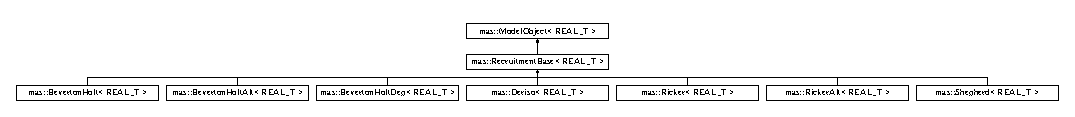
\includegraphics[height=1.121495cm]{structmas_1_1_recruitment_base}
\end{center}
\end{figure}
\subsection*{Public Types}
\begin{DoxyCompactItemize}
\item 
typedef \hyperlink{structmas_1_1_variable_trait}{mas\-::\-Variable\-Trait}\\*
$<$ R\-E\-A\-L\-\_\-\-T $>$\-::\hyperlink{structmas_1_1_recruitment_base_acc579cce5a745bcbb31758b3420c960b}{variable} \hyperlink{structmas_1_1_recruitment_base_acc579cce5a745bcbb31758b3420c960b}{variable}
\end{DoxyCompactItemize}
\subsection*{Public Member Functions}
\begin{DoxyCompactItemize}
\item 
virtual const \hyperlink{structmas_1_1_recruitment_base_acc579cce5a745bcbb31758b3420c960b}{variable} \hyperlink{structmas_1_1_recruitment_base_a74a7f9dd7090f156c6a5068ce29f53ff}{Evaluate} (const int \&pop\-\_\-id, const int \&area\-\_\-id, const \hyperlink{structmas_1_1_recruitment_base_acc579cce5a745bcbb31758b3420c960b}{variable} \&s)=0
\item 
std\-::string \hyperlink{structmas_1_1_recruitment_base_abbfe6d0214fd35a775027ad54e3d10f6}{Recruit\-Deviations\-To\-J\-S\-O\-N} ()
\item 
virtual const std\-::string \hyperlink{structmas_1_1_recruitment_base_abfdd47e97127a35f81d441ac3e1afaec}{Name} ()
\item 
void \hyperlink{structmas_1_1_recruitment_base_a6cb0c256e576b95deebc997bd5aa6b64}{Prepare} ()
\end{DoxyCompactItemize}
\subsection*{Public Attributes}
\begin{DoxyCompactItemize}
\item 
\hyperlink{structmas_1_1_recruitment_base_acc579cce5a745bcbb31758b3420c960b}{variable} \hyperlink{structmas_1_1_recruitment_base_a4f99fb299e8f00f36645ffb032592e04}{R0}
\item 
\hyperlink{structmas_1_1_recruitment_base_acc579cce5a745bcbb31758b3420c960b}{variable} \hyperlink{structmas_1_1_recruitment_base_ac460098ea97bddb9f1a41bb854d8f89d}{h}
\item 
\hyperlink{structmas_1_1_recruitment_base_acc579cce5a745bcbb31758b3420c960b}{variable} \hyperlink{structmas_1_1_recruitment_base_a17d973c0bbb663b2d836c9f5b1270b9b}{sigma\-\_\-r}
\item 
\hyperlink{structmas_1_1_recruitment_base_acc579cce5a745bcbb31758b3420c960b}{variable} \hyperlink{structmas_1_1_recruitment_base_a85904d0c8996b9903609f6f9a93d20bc}{rho}
\item 
std\-::unordered\-\_\-map$<$ int, \\*
std\-::unordered\-\_\-map$<$ int, \\*
\hyperlink{structmas_1_1_recruitment_base_acc579cce5a745bcbb31758b3420c960b}{variable} $>$ $>$ \hyperlink{structmas_1_1_recruitment_base_ab682c3efec8a1c9ffe3481f193ef6d64}{S\-B0}
\item 
\hyperlink{structmas_1_1_recruitment_base_acc579cce5a745bcbb31758b3420c960b}{variable} \hyperlink{structmas_1_1_recruitment_base_a4e6c20c02bc08e1ca5f3489992fd8c2f}{phi0}
\item 
std\-::vector$<$ \hyperlink{structmas_1_1_recruitment_base_acc579cce5a745bcbb31758b3420c960b}{variable} $>$ \hyperlink{structmas_1_1_recruitment_base_acab1229c5bea140584480dee25e28414}{recruitment\-\_\-deviations}
\item 
bool \hyperlink{structmas_1_1_recruitment_base_a84eb1f6997fa59d983ba24a1d2d36f5e}{estimating\-\_\-recruitment\-\_\-deviations} = false
\end{DoxyCompactItemize}


\subsection{Detailed Description}
\subsubsection*{template$<$typename R\-E\-A\-L\-\_\-\-T$>$struct mas\-::\-Recruitment\-Base$<$ R\-E\-A\-L\-\_\-\-T $>$}



Definition at line 39 of file Recruitment.\-hpp.



\subsection{Member Typedef Documentation}
\hypertarget{structmas_1_1_recruitment_base_acc579cce5a745bcbb31758b3420c960b}{\index{mas\-::\-Recruitment\-Base@{mas\-::\-Recruitment\-Base}!variable@{variable}}
\index{variable@{variable}!mas::RecruitmentBase@{mas\-::\-Recruitment\-Base}}
\subsubsection[{variable}]{\setlength{\rightskip}{0pt plus 5cm}template$<$typename R\-E\-A\-L\-\_\-\-T $>$ typedef {\bf mas\-::\-Variable\-Trait}$<$R\-E\-A\-L\-\_\-\-T$>$\-::{\bf variable} {\bf mas\-::\-Recruitment\-Base}$<$ R\-E\-A\-L\-\_\-\-T $>$\-::{\bf variable}}}\label{structmas_1_1_recruitment_base_acc579cce5a745bcbb31758b3420c960b}


Definition at line 40 of file Recruitment.\-hpp.



\subsection{Member Function Documentation}
\hypertarget{structmas_1_1_recruitment_base_a74a7f9dd7090f156c6a5068ce29f53ff}{\index{mas\-::\-Recruitment\-Base@{mas\-::\-Recruitment\-Base}!Evaluate@{Evaluate}}
\index{Evaluate@{Evaluate}!mas::RecruitmentBase@{mas\-::\-Recruitment\-Base}}
\subsubsection[{Evaluate}]{\setlength{\rightskip}{0pt plus 5cm}template$<$typename R\-E\-A\-L\-\_\-\-T $>$ virtual const {\bf variable} {\bf mas\-::\-Recruitment\-Base}$<$ R\-E\-A\-L\-\_\-\-T $>$\-::Evaluate (
\begin{DoxyParamCaption}
\item[{const int \&}]{pop\-\_\-id, }
\item[{const int \&}]{area\-\_\-id, }
\item[{const {\bf variable} \&}]{s}
\end{DoxyParamCaption}
)\hspace{0.3cm}{\ttfamily [pure virtual]}}}\label{structmas_1_1_recruitment_base_a74a7f9dd7090f156c6a5068ce29f53ff}


Implemented in \hyperlink{structmas_1_1_deriso_a056c98851c0b002b87c31b8b4a660fde}{mas\-::\-Deriso$<$ R\-E\-A\-L\-\_\-\-T $>$}, \hyperlink{structmas_1_1_shepherd_a0e7a914d27be18b2c9efa052958d1f0b}{mas\-::\-Shepherd$<$ R\-E\-A\-L\-\_\-\-T $>$}, \hyperlink{structmas_1_1_beverton_holt_dep_a9433b67c120c398d05c3f900db44f985}{mas\-::\-Beverton\-Holt\-Dep$<$ R\-E\-A\-L\-\_\-\-T $>$}, \hyperlink{structmas_1_1_beverton_holt_alt_abce4e13656f770710ed047efa1e78ae0}{mas\-::\-Beverton\-Holt\-Alt$<$ R\-E\-A\-L\-\_\-\-T $>$}, \hyperlink{structmas_1_1_beverton_holt_a2fbd4bf3841b23145fc9000fac124818}{mas\-::\-Beverton\-Holt$<$ R\-E\-A\-L\-\_\-\-T $>$}, \hyperlink{structmas_1_1_ricker_alt_a856496f34bee8e696a55a5960edd5b4e}{mas\-::\-Ricker\-Alt$<$ R\-E\-A\-L\-\_\-\-T $>$}, and \hyperlink{structmas_1_1_ricker_ab5b9063ac4db823f6d6413a336dc3dc2}{mas\-::\-Ricker$<$ R\-E\-A\-L\-\_\-\-T $>$}.

\hypertarget{structmas_1_1_recruitment_base_abfdd47e97127a35f81d441ac3e1afaec}{\index{mas\-::\-Recruitment\-Base@{mas\-::\-Recruitment\-Base}!Name@{Name}}
\index{Name@{Name}!mas::RecruitmentBase@{mas\-::\-Recruitment\-Base}}
\subsubsection[{Name}]{\setlength{\rightskip}{0pt plus 5cm}template$<$typename R\-E\-A\-L\-\_\-\-T $>$ virtual const std\-::string {\bf mas\-::\-Recruitment\-Base}$<$ R\-E\-A\-L\-\_\-\-T $>$\-::Name (
\begin{DoxyParamCaption}
{}
\end{DoxyParamCaption}
)\hspace{0.3cm}{\ttfamily [inline]}, {\ttfamily [virtual]}}}\label{structmas_1_1_recruitment_base_abfdd47e97127a35f81d441ac3e1afaec}


Reimplemented in \hyperlink{structmas_1_1_deriso_a4bd2deff5d9d3cac9e90941df9881b29}{mas\-::\-Deriso$<$ R\-E\-A\-L\-\_\-\-T $>$}, \hyperlink{structmas_1_1_shepherd_aed20558dd1e310073ebba7968fe5f36f}{mas\-::\-Shepherd$<$ R\-E\-A\-L\-\_\-\-T $>$}, \hyperlink{structmas_1_1_beverton_holt_dep_ac389fdb4eb88ccd663ec47a854d703d1}{mas\-::\-Beverton\-Holt\-Dep$<$ R\-E\-A\-L\-\_\-\-T $>$}, \hyperlink{structmas_1_1_beverton_holt_alt_a69b3da75fcea33be0ce8b12f6448b3b0}{mas\-::\-Beverton\-Holt\-Alt$<$ R\-E\-A\-L\-\_\-\-T $>$}, \hyperlink{structmas_1_1_beverton_holt_aa6e6f7fa8edecf211eedee2d2219c3ce}{mas\-::\-Beverton\-Holt$<$ R\-E\-A\-L\-\_\-\-T $>$}, \hyperlink{structmas_1_1_ricker_alt_a35f2678bc6e8c8b32691daca09bcca93}{mas\-::\-Ricker\-Alt$<$ R\-E\-A\-L\-\_\-\-T $>$}, and \hyperlink{structmas_1_1_ricker_a7628e704459668064aeab604c223ebb5}{mas\-::\-Ricker$<$ R\-E\-A\-L\-\_\-\-T $>$}.



Definition at line 74 of file Recruitment.\-hpp.

\hypertarget{structmas_1_1_recruitment_base_a6cb0c256e576b95deebc997bd5aa6b64}{\index{mas\-::\-Recruitment\-Base@{mas\-::\-Recruitment\-Base}!Prepare@{Prepare}}
\index{Prepare@{Prepare}!mas::RecruitmentBase@{mas\-::\-Recruitment\-Base}}
\subsubsection[{Prepare}]{\setlength{\rightskip}{0pt plus 5cm}template$<$typename R\-E\-A\-L\-\_\-\-T $>$ void {\bf mas\-::\-Recruitment\-Base}$<$ R\-E\-A\-L\-\_\-\-T $>$\-::Prepare (
\begin{DoxyParamCaption}
{}
\end{DoxyParamCaption}
)\hspace{0.3cm}{\ttfamily [inline]}}}\label{structmas_1_1_recruitment_base_a6cb0c256e576b95deebc997bd5aa6b64}


Definition at line 78 of file Recruitment.\-hpp.

\hypertarget{structmas_1_1_recruitment_base_abbfe6d0214fd35a775027ad54e3d10f6}{\index{mas\-::\-Recruitment\-Base@{mas\-::\-Recruitment\-Base}!Recruit\-Deviations\-To\-J\-S\-O\-N@{Recruit\-Deviations\-To\-J\-S\-O\-N}}
\index{Recruit\-Deviations\-To\-J\-S\-O\-N@{Recruit\-Deviations\-To\-J\-S\-O\-N}!mas::RecruitmentBase@{mas\-::\-Recruitment\-Base}}
\subsubsection[{Recruit\-Deviations\-To\-J\-S\-O\-N}]{\setlength{\rightskip}{0pt plus 5cm}template$<$typename R\-E\-A\-L\-\_\-\-T $>$ std\-::string {\bf mas\-::\-Recruitment\-Base}$<$ R\-E\-A\-L\-\_\-\-T $>$\-::Recruit\-Deviations\-To\-J\-S\-O\-N (
\begin{DoxyParamCaption}
{}
\end{DoxyParamCaption}
)\hspace{0.3cm}{\ttfamily [inline]}}}\label{structmas_1_1_recruitment_base_abbfe6d0214fd35a775027ad54e3d10f6}


Definition at line 54 of file Recruitment.\-hpp.



\subsection{Member Data Documentation}
\hypertarget{structmas_1_1_recruitment_base_a84eb1f6997fa59d983ba24a1d2d36f5e}{\index{mas\-::\-Recruitment\-Base@{mas\-::\-Recruitment\-Base}!estimating\-\_\-recruitment\-\_\-deviations@{estimating\-\_\-recruitment\-\_\-deviations}}
\index{estimating\-\_\-recruitment\-\_\-deviations@{estimating\-\_\-recruitment\-\_\-deviations}!mas::RecruitmentBase@{mas\-::\-Recruitment\-Base}}
\subsubsection[{estimating\-\_\-recruitment\-\_\-deviations}]{\setlength{\rightskip}{0pt plus 5cm}template$<$typename R\-E\-A\-L\-\_\-\-T $>$ bool {\bf mas\-::\-Recruitment\-Base}$<$ R\-E\-A\-L\-\_\-\-T $>$\-::estimating\-\_\-recruitment\-\_\-deviations = false}}\label{structmas_1_1_recruitment_base_a84eb1f6997fa59d983ba24a1d2d36f5e}


Definition at line 50 of file Recruitment.\-hpp.

\hypertarget{structmas_1_1_recruitment_base_ac460098ea97bddb9f1a41bb854d8f89d}{\index{mas\-::\-Recruitment\-Base@{mas\-::\-Recruitment\-Base}!h@{h}}
\index{h@{h}!mas::RecruitmentBase@{mas\-::\-Recruitment\-Base}}
\subsubsection[{h}]{\setlength{\rightskip}{0pt plus 5cm}template$<$typename R\-E\-A\-L\-\_\-\-T $>$ {\bf variable} {\bf mas\-::\-Recruitment\-Base}$<$ R\-E\-A\-L\-\_\-\-T $>$\-::h}}\label{structmas_1_1_recruitment_base_ac460098ea97bddb9f1a41bb854d8f89d}


Definition at line 42 of file Recruitment.\-hpp.

\hypertarget{structmas_1_1_recruitment_base_a4e6c20c02bc08e1ca5f3489992fd8c2f}{\index{mas\-::\-Recruitment\-Base@{mas\-::\-Recruitment\-Base}!phi0@{phi0}}
\index{phi0@{phi0}!mas::RecruitmentBase@{mas\-::\-Recruitment\-Base}}
\subsubsection[{phi0}]{\setlength{\rightskip}{0pt plus 5cm}template$<$typename R\-E\-A\-L\-\_\-\-T $>$ {\bf variable} {\bf mas\-::\-Recruitment\-Base}$<$ R\-E\-A\-L\-\_\-\-T $>$\-::phi0}}\label{structmas_1_1_recruitment_base_a4e6c20c02bc08e1ca5f3489992fd8c2f}


Definition at line 47 of file Recruitment.\-hpp.

\hypertarget{structmas_1_1_recruitment_base_a4f99fb299e8f00f36645ffb032592e04}{\index{mas\-::\-Recruitment\-Base@{mas\-::\-Recruitment\-Base}!R0@{R0}}
\index{R0@{R0}!mas::RecruitmentBase@{mas\-::\-Recruitment\-Base}}
\subsubsection[{R0}]{\setlength{\rightskip}{0pt plus 5cm}template$<$typename R\-E\-A\-L\-\_\-\-T $>$ {\bf variable} {\bf mas\-::\-Recruitment\-Base}$<$ R\-E\-A\-L\-\_\-\-T $>$\-::R0}}\label{structmas_1_1_recruitment_base_a4f99fb299e8f00f36645ffb032592e04}


Definition at line 41 of file Recruitment.\-hpp.

\hypertarget{structmas_1_1_recruitment_base_acab1229c5bea140584480dee25e28414}{\index{mas\-::\-Recruitment\-Base@{mas\-::\-Recruitment\-Base}!recruitment\-\_\-deviations@{recruitment\-\_\-deviations}}
\index{recruitment\-\_\-deviations@{recruitment\-\_\-deviations}!mas::RecruitmentBase@{mas\-::\-Recruitment\-Base}}
\subsubsection[{recruitment\-\_\-deviations}]{\setlength{\rightskip}{0pt plus 5cm}template$<$typename R\-E\-A\-L\-\_\-\-T $>$ std\-::vector$<${\bf variable}$>$ {\bf mas\-::\-Recruitment\-Base}$<$ R\-E\-A\-L\-\_\-\-T $>$\-::recruitment\-\_\-deviations}}\label{structmas_1_1_recruitment_base_acab1229c5bea140584480dee25e28414}


Definition at line 49 of file Recruitment.\-hpp.

\hypertarget{structmas_1_1_recruitment_base_a85904d0c8996b9903609f6f9a93d20bc}{\index{mas\-::\-Recruitment\-Base@{mas\-::\-Recruitment\-Base}!rho@{rho}}
\index{rho@{rho}!mas::RecruitmentBase@{mas\-::\-Recruitment\-Base}}
\subsubsection[{rho}]{\setlength{\rightskip}{0pt plus 5cm}template$<$typename R\-E\-A\-L\-\_\-\-T $>$ {\bf variable} {\bf mas\-::\-Recruitment\-Base}$<$ R\-E\-A\-L\-\_\-\-T $>$\-::rho}}\label{structmas_1_1_recruitment_base_a85904d0c8996b9903609f6f9a93d20bc}


Definition at line 44 of file Recruitment.\-hpp.

\hypertarget{structmas_1_1_recruitment_base_ab682c3efec8a1c9ffe3481f193ef6d64}{\index{mas\-::\-Recruitment\-Base@{mas\-::\-Recruitment\-Base}!S\-B0@{S\-B0}}
\index{S\-B0@{S\-B0}!mas::RecruitmentBase@{mas\-::\-Recruitment\-Base}}
\subsubsection[{S\-B0}]{\setlength{\rightskip}{0pt plus 5cm}template$<$typename R\-E\-A\-L\-\_\-\-T $>$ std\-::unordered\-\_\-map$<$int, std\-::unordered\-\_\-map$<$int, {\bf variable}$>$ $>$ {\bf mas\-::\-Recruitment\-Base}$<$ R\-E\-A\-L\-\_\-\-T $>$\-::S\-B0}}\label{structmas_1_1_recruitment_base_ab682c3efec8a1c9ffe3481f193ef6d64}


Definition at line 46 of file Recruitment.\-hpp.

\hypertarget{structmas_1_1_recruitment_base_a17d973c0bbb663b2d836c9f5b1270b9b}{\index{mas\-::\-Recruitment\-Base@{mas\-::\-Recruitment\-Base}!sigma\-\_\-r@{sigma\-\_\-r}}
\index{sigma\-\_\-r@{sigma\-\_\-r}!mas::RecruitmentBase@{mas\-::\-Recruitment\-Base}}
\subsubsection[{sigma\-\_\-r}]{\setlength{\rightskip}{0pt plus 5cm}template$<$typename R\-E\-A\-L\-\_\-\-T $>$ {\bf variable} {\bf mas\-::\-Recruitment\-Base}$<$ R\-E\-A\-L\-\_\-\-T $>$\-::sigma\-\_\-r}}\label{structmas_1_1_recruitment_base_a17d973c0bbb663b2d836c9f5b1270b9b}


Definition at line 43 of file Recruitment.\-hpp.



The documentation for this struct was generated from the following file\-:\begin{DoxyCompactItemize}
\item 
/home/oppy/\-Net\-Beans\-Projects/mas/\hyperlink{_recruitment_8hpp}{Recruitment.\-hpp}\end{DoxyCompactItemize}

\hypertarget{structmas_1_1_ricker}{\section{mas\-:\-:Ricker$<$ R\-E\-A\-L\-\_\-\-T $>$ Struct Template Reference}
\label{structmas_1_1_ricker}\index{mas\-::\-Ricker$<$ R\-E\-A\-L\-\_\-\-T $>$@{mas\-::\-Ricker$<$ R\-E\-A\-L\-\_\-\-T $>$}}
}


{\ttfamily \#include $<$Recruitment.\-hpp$>$}

Inheritance diagram for mas\-:\-:Ricker$<$ R\-E\-A\-L\-\_\-\-T $>$\-:\begin{figure}[H]
\begin{center}
\leavevmode
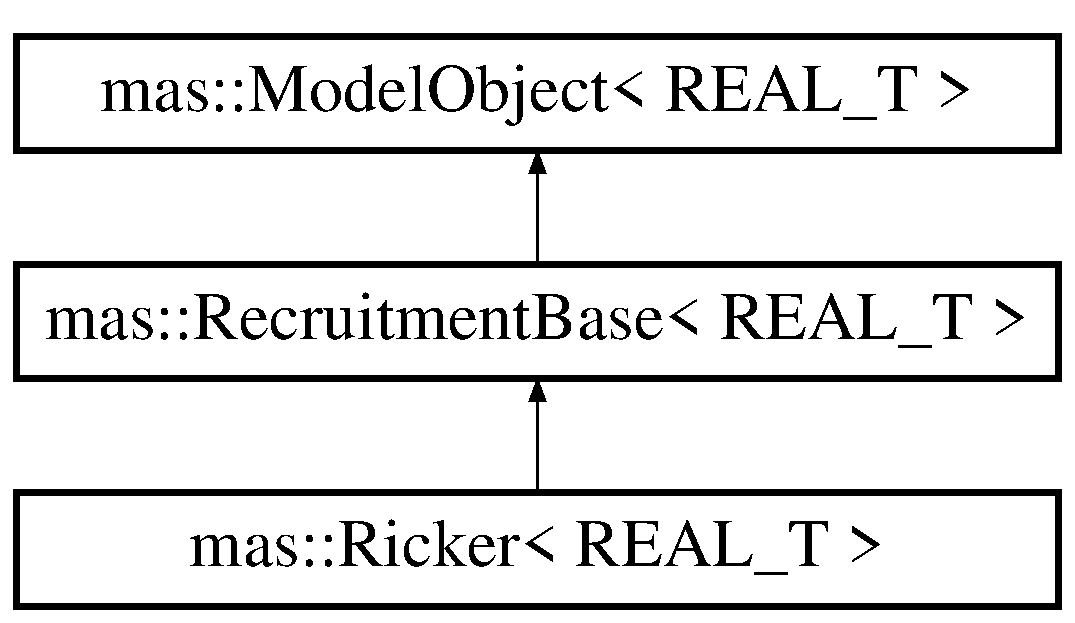
\includegraphics[height=3.000000cm]{structmas_1_1_ricker}
\end{center}
\end{figure}
\subsection*{Public Types}
\begin{DoxyCompactItemize}
\item 
typedef \hyperlink{structmas_1_1_variable_trait}{Variable\-Trait}$<$ R\-E\-A\-L\-\_\-\-T $>$\\*
\-::\hyperlink{structmas_1_1_ricker_a1e7489f196696277bb4c4fab0b5db240}{variable} \hyperlink{structmas_1_1_ricker_a1e7489f196696277bb4c4fab0b5db240}{variable}
\end{DoxyCompactItemize}
\subsection*{Public Member Functions}
\begin{DoxyCompactItemize}
\item 
const \hyperlink{structmas_1_1_ricker_a1e7489f196696277bb4c4fab0b5db240}{variable} \hyperlink{structmas_1_1_ricker_ab5b9063ac4db823f6d6413a336dc3dc2}{Evaluate} (const int \&pop\-\_\-id, const int \&area\-\_\-id, const \hyperlink{structmas_1_1_ricker_a1e7489f196696277bb4c4fab0b5db240}{variable} \&s)
\item 
virtual const std\-::string \hyperlink{structmas_1_1_ricker_af6cb56b70e0449cfb5fdfab757971560}{To\-J\-S\-O\-N\-String} ()
\item 
virtual const std\-::string \hyperlink{structmas_1_1_ricker_a7628e704459668064aeab604c223ebb5}{Name} ()
\end{DoxyCompactItemize}
\subsection*{Public Attributes}
\begin{DoxyCompactItemize}
\item 
\hyperlink{structmas_1_1_ricker_a1e7489f196696277bb4c4fab0b5db240}{variable} \hyperlink{structmas_1_1_ricker_a50aa86b70525d2103514d9bf4152b130}{alpha}
\item 
\hyperlink{structmas_1_1_ricker_a1e7489f196696277bb4c4fab0b5db240}{variable} \hyperlink{structmas_1_1_ricker_ac3ac0028bef4f094b30861c4bef9f5b8}{beta}
\end{DoxyCompactItemize}


\subsection{Detailed Description}
\subsubsection*{template$<$typename R\-E\-A\-L\-\_\-\-T$>$struct mas\-::\-Ricker$<$ R\-E\-A\-L\-\_\-\-T $>$}



Definition at line 93 of file Recruitment.\-hpp.



\subsection{Member Typedef Documentation}
\hypertarget{structmas_1_1_ricker_a1e7489f196696277bb4c4fab0b5db240}{\index{mas\-::\-Ricker@{mas\-::\-Ricker}!variable@{variable}}
\index{variable@{variable}!mas::Ricker@{mas\-::\-Ricker}}
\subsubsection[{variable}]{\setlength{\rightskip}{0pt plus 5cm}template$<$typename R\-E\-A\-L\-\_\-\-T $>$ typedef {\bf Variable\-Trait}$<$R\-E\-A\-L\-\_\-\-T$>$\-::{\bf variable} {\bf mas\-::\-Ricker}$<$ R\-E\-A\-L\-\_\-\-T $>$\-::{\bf variable}}}\label{structmas_1_1_ricker_a1e7489f196696277bb4c4fab0b5db240}


Definition at line 94 of file Recruitment.\-hpp.



\subsection{Member Function Documentation}
\hypertarget{structmas_1_1_ricker_ab5b9063ac4db823f6d6413a336dc3dc2}{\index{mas\-::\-Ricker@{mas\-::\-Ricker}!Evaluate@{Evaluate}}
\index{Evaluate@{Evaluate}!mas::Ricker@{mas\-::\-Ricker}}
\subsubsection[{Evaluate}]{\setlength{\rightskip}{0pt plus 5cm}template$<$typename R\-E\-A\-L\-\_\-\-T $>$ const {\bf variable} {\bf mas\-::\-Ricker}$<$ R\-E\-A\-L\-\_\-\-T $>$\-::Evaluate (
\begin{DoxyParamCaption}
\item[{const int \&}]{pop\-\_\-id, }
\item[{const int \&}]{area\-\_\-id, }
\item[{const {\bf variable} \&}]{s}
\end{DoxyParamCaption}
)\hspace{0.3cm}{\ttfamily [inline]}, {\ttfamily [virtual]}}}\label{structmas_1_1_ricker_ab5b9063ac4db823f6d6413a336dc3dc2}


Implements \hyperlink{structmas_1_1_recruitment_base_a74a7f9dd7090f156c6a5068ce29f53ff}{mas\-::\-Recruitment\-Base$<$ R\-E\-A\-L\-\_\-\-T $>$}.



Definition at line 98 of file Recruitment.\-hpp.

\hypertarget{structmas_1_1_ricker_a7628e704459668064aeab604c223ebb5}{\index{mas\-::\-Ricker@{mas\-::\-Ricker}!Name@{Name}}
\index{Name@{Name}!mas::Ricker@{mas\-::\-Ricker}}
\subsubsection[{Name}]{\setlength{\rightskip}{0pt plus 5cm}template$<$typename R\-E\-A\-L\-\_\-\-T $>$ virtual const std\-::string {\bf mas\-::\-Ricker}$<$ R\-E\-A\-L\-\_\-\-T $>$\-::Name (
\begin{DoxyParamCaption}
{}
\end{DoxyParamCaption}
)\hspace{0.3cm}{\ttfamily [inline]}, {\ttfamily [virtual]}}}\label{structmas_1_1_ricker_a7628e704459668064aeab604c223ebb5}


Reimplemented from \hyperlink{structmas_1_1_recruitment_base_abfdd47e97127a35f81d441ac3e1afaec}{mas\-::\-Recruitment\-Base$<$ R\-E\-A\-L\-\_\-\-T $>$}.



Definition at line 121 of file Recruitment.\-hpp.

\hypertarget{structmas_1_1_ricker_af6cb56b70e0449cfb5fdfab757971560}{\index{mas\-::\-Ricker@{mas\-::\-Ricker}!To\-J\-S\-O\-N\-String@{To\-J\-S\-O\-N\-String}}
\index{To\-J\-S\-O\-N\-String@{To\-J\-S\-O\-N\-String}!mas::Ricker@{mas\-::\-Ricker}}
\subsubsection[{To\-J\-S\-O\-N\-String}]{\setlength{\rightskip}{0pt plus 5cm}template$<$typename R\-E\-A\-L\-\_\-\-T $>$ virtual const std\-::string {\bf mas\-::\-Ricker}$<$ R\-E\-A\-L\-\_\-\-T $>$\-::To\-J\-S\-O\-N\-String (
\begin{DoxyParamCaption}
{}
\end{DoxyParamCaption}
)\hspace{0.3cm}{\ttfamily [inline]}, {\ttfamily [virtual]}}}\label{structmas_1_1_ricker_af6cb56b70e0449cfb5fdfab757971560}


Reimplemented from \hyperlink{structmas_1_1_model_object_af40b3c89b11919fc5aea21dcf1cd027b}{mas\-::\-Model\-Object$<$ R\-E\-A\-L\-\_\-\-T $>$}.



Definition at line 102 of file Recruitment.\-hpp.



\subsection{Member Data Documentation}
\hypertarget{structmas_1_1_ricker_a50aa86b70525d2103514d9bf4152b130}{\index{mas\-::\-Ricker@{mas\-::\-Ricker}!alpha@{alpha}}
\index{alpha@{alpha}!mas::Ricker@{mas\-::\-Ricker}}
\subsubsection[{alpha}]{\setlength{\rightskip}{0pt plus 5cm}template$<$typename R\-E\-A\-L\-\_\-\-T $>$ {\bf variable} {\bf mas\-::\-Ricker}$<$ R\-E\-A\-L\-\_\-\-T $>$\-::alpha}}\label{structmas_1_1_ricker_a50aa86b70525d2103514d9bf4152b130}


Definition at line 95 of file Recruitment.\-hpp.

\hypertarget{structmas_1_1_ricker_ac3ac0028bef4f094b30861c4bef9f5b8}{\index{mas\-::\-Ricker@{mas\-::\-Ricker}!beta@{beta}}
\index{beta@{beta}!mas::Ricker@{mas\-::\-Ricker}}
\subsubsection[{beta}]{\setlength{\rightskip}{0pt plus 5cm}template$<$typename R\-E\-A\-L\-\_\-\-T $>$ {\bf variable} {\bf mas\-::\-Ricker}$<$ R\-E\-A\-L\-\_\-\-T $>$\-::beta}}\label{structmas_1_1_ricker_ac3ac0028bef4f094b30861c4bef9f5b8}


Definition at line 96 of file Recruitment.\-hpp.



The documentation for this struct was generated from the following file\-:\begin{DoxyCompactItemize}
\item 
/home/oppy/\-Net\-Beans\-Projects/mas/\hyperlink{_recruitment_8hpp}{Recruitment.\-hpp}\end{DoxyCompactItemize}

\hypertarget{structmas_1_1_ricker_alt}{\section{mas\-:\-:Ricker\-Alt$<$ R\-E\-A\-L\-\_\-\-T $>$ Struct Template Reference}
\label{structmas_1_1_ricker_alt}\index{mas\-::\-Ricker\-Alt$<$ R\-E\-A\-L\-\_\-\-T $>$@{mas\-::\-Ricker\-Alt$<$ R\-E\-A\-L\-\_\-\-T $>$}}
}


{\ttfamily \#include $<$Recruitment.\-hpp$>$}

Inheritance diagram for mas\-:\-:Ricker\-Alt$<$ R\-E\-A\-L\-\_\-\-T $>$\-:\begin{figure}[H]
\begin{center}
\leavevmode
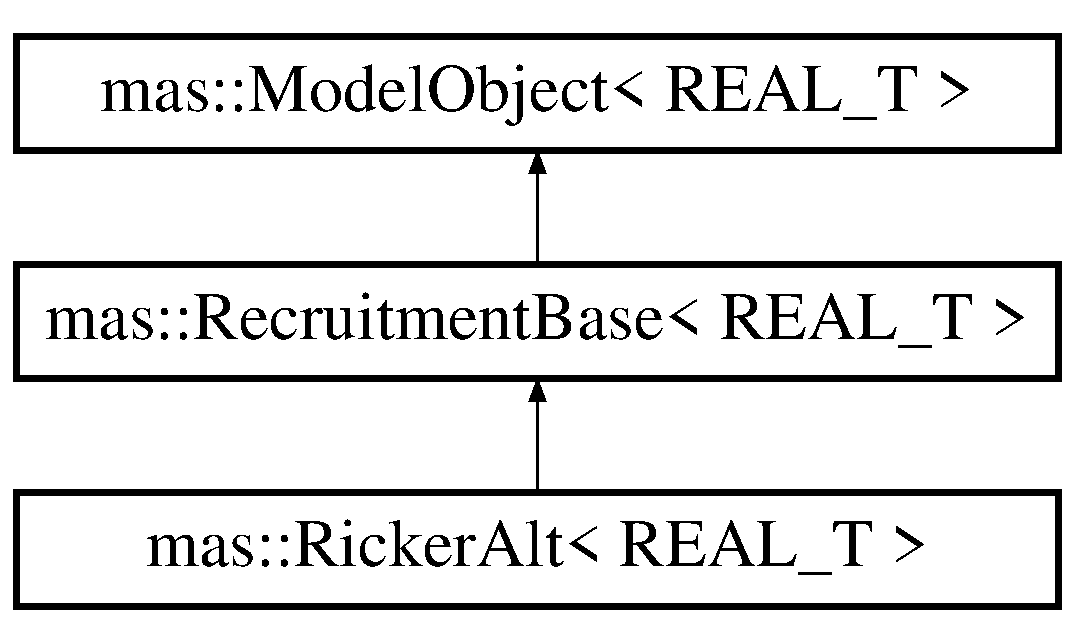
\includegraphics[height=3.000000cm]{structmas_1_1_ricker_alt}
\end{center}
\end{figure}
\subsection*{Public Types}
\begin{DoxyCompactItemize}
\item 
typedef \hyperlink{structmas_1_1_variable_trait}{Variable\-Trait}$<$ R\-E\-A\-L\-\_\-\-T $>$\\*
\-::\hyperlink{structmas_1_1_ricker_alt_a3f6410d01fd55ca163120cb17b862cd8}{variable} \hyperlink{structmas_1_1_ricker_alt_a3f6410d01fd55ca163120cb17b862cd8}{variable}
\end{DoxyCompactItemize}
\subsection*{Public Member Functions}
\begin{DoxyCompactItemize}
\item 
const \hyperlink{structmas_1_1_ricker_alt_a3f6410d01fd55ca163120cb17b862cd8}{variable} \hyperlink{structmas_1_1_ricker_alt_a856496f34bee8e696a55a5960edd5b4e}{Evaluate} (const int \&pop\-\_\-id, const int \&area\-\_\-id, const \hyperlink{structmas_1_1_ricker_alt_a3f6410d01fd55ca163120cb17b862cd8}{variable} \&s)
\item 
virtual const std\-::string \hyperlink{structmas_1_1_ricker_alt_a76187fc316998d57d245c189560bcade}{To\-J\-S\-O\-N\-String} ()
\item 
virtual const std\-::string \hyperlink{structmas_1_1_ricker_alt_a35f2678bc6e8c8b32691daca09bcca93}{Name} ()
\end{DoxyCompactItemize}
\subsection*{Public Attributes}
\begin{DoxyCompactItemize}
\item 
\hyperlink{structmas_1_1_ricker_alt_a3f6410d01fd55ca163120cb17b862cd8}{variable} \hyperlink{structmas_1_1_ricker_alt_a64d1ad551ce910d6ccab77e80c3a217a}{phi0}
\item 
\hyperlink{structmas_1_1_ricker_alt_a3f6410d01fd55ca163120cb17b862cd8}{variable} \hyperlink{structmas_1_1_ricker_alt_a17b23c9c97b4e4992afafcca81062db8}{A}
\end{DoxyCompactItemize}


\subsection{Detailed Description}
\subsubsection*{template$<$typename R\-E\-A\-L\-\_\-\-T$>$struct mas\-::\-Ricker\-Alt$<$ R\-E\-A\-L\-\_\-\-T $>$}



Definition at line 127 of file Recruitment.\-hpp.



\subsection{Member Typedef Documentation}
\hypertarget{structmas_1_1_ricker_alt_a3f6410d01fd55ca163120cb17b862cd8}{\index{mas\-::\-Ricker\-Alt@{mas\-::\-Ricker\-Alt}!variable@{variable}}
\index{variable@{variable}!mas::RickerAlt@{mas\-::\-Ricker\-Alt}}
\subsubsection[{variable}]{\setlength{\rightskip}{0pt plus 5cm}template$<$typename R\-E\-A\-L\-\_\-\-T $>$ typedef {\bf Variable\-Trait}$<$R\-E\-A\-L\-\_\-\-T$>$\-::{\bf variable} {\bf mas\-::\-Ricker\-Alt}$<$ R\-E\-A\-L\-\_\-\-T $>$\-::{\bf variable}}}\label{structmas_1_1_ricker_alt_a3f6410d01fd55ca163120cb17b862cd8}


Definition at line 128 of file Recruitment.\-hpp.



\subsection{Member Function Documentation}
\hypertarget{structmas_1_1_ricker_alt_a856496f34bee8e696a55a5960edd5b4e}{\index{mas\-::\-Ricker\-Alt@{mas\-::\-Ricker\-Alt}!Evaluate@{Evaluate}}
\index{Evaluate@{Evaluate}!mas::RickerAlt@{mas\-::\-Ricker\-Alt}}
\subsubsection[{Evaluate}]{\setlength{\rightskip}{0pt plus 5cm}template$<$typename R\-E\-A\-L\-\_\-\-T $>$ const {\bf variable} {\bf mas\-::\-Ricker\-Alt}$<$ R\-E\-A\-L\-\_\-\-T $>$\-::Evaluate (
\begin{DoxyParamCaption}
\item[{const int \&}]{pop\-\_\-id, }
\item[{const int \&}]{area\-\_\-id, }
\item[{const {\bf variable} \&}]{s}
\end{DoxyParamCaption}
)\hspace{0.3cm}{\ttfamily [inline]}, {\ttfamily [virtual]}}}\label{structmas_1_1_ricker_alt_a856496f34bee8e696a55a5960edd5b4e}
Alternative \hyperlink{structmas_1_1_ricker}{Ricker} Spawn-\/\-Recruit relationship 
\begin{DoxyParams}{Parameters}
{\em s} & -\/ spawning biomass or abundance \\
\hline
\end{DoxyParams}
\begin{DoxyReturn}{Returns}

\end{DoxyReturn}


Implements \hyperlink{structmas_1_1_recruitment_base_a74a7f9dd7090f156c6a5068ce29f53ff}{mas\-::\-Recruitment\-Base$<$ R\-E\-A\-L\-\_\-\-T $>$}.



Definition at line 137 of file Recruitment.\-hpp.

\hypertarget{structmas_1_1_ricker_alt_a35f2678bc6e8c8b32691daca09bcca93}{\index{mas\-::\-Ricker\-Alt@{mas\-::\-Ricker\-Alt}!Name@{Name}}
\index{Name@{Name}!mas::RickerAlt@{mas\-::\-Ricker\-Alt}}
\subsubsection[{Name}]{\setlength{\rightskip}{0pt plus 5cm}template$<$typename R\-E\-A\-L\-\_\-\-T $>$ virtual const std\-::string {\bf mas\-::\-Ricker\-Alt}$<$ R\-E\-A\-L\-\_\-\-T $>$\-::Name (
\begin{DoxyParamCaption}
{}
\end{DoxyParamCaption}
)\hspace{0.3cm}{\ttfamily [inline]}, {\ttfamily [virtual]}}}\label{structmas_1_1_ricker_alt_a35f2678bc6e8c8b32691daca09bcca93}


Reimplemented from \hyperlink{structmas_1_1_recruitment_base_abfdd47e97127a35f81d441ac3e1afaec}{mas\-::\-Recruitment\-Base$<$ R\-E\-A\-L\-\_\-\-T $>$}.



Definition at line 161 of file Recruitment.\-hpp.

\hypertarget{structmas_1_1_ricker_alt_a76187fc316998d57d245c189560bcade}{\index{mas\-::\-Ricker\-Alt@{mas\-::\-Ricker\-Alt}!To\-J\-S\-O\-N\-String@{To\-J\-S\-O\-N\-String}}
\index{To\-J\-S\-O\-N\-String@{To\-J\-S\-O\-N\-String}!mas::RickerAlt@{mas\-::\-Ricker\-Alt}}
\subsubsection[{To\-J\-S\-O\-N\-String}]{\setlength{\rightskip}{0pt plus 5cm}template$<$typename R\-E\-A\-L\-\_\-\-T $>$ virtual const std\-::string {\bf mas\-::\-Ricker\-Alt}$<$ R\-E\-A\-L\-\_\-\-T $>$\-::To\-J\-S\-O\-N\-String (
\begin{DoxyParamCaption}
{}
\end{DoxyParamCaption}
)\hspace{0.3cm}{\ttfamily [inline]}, {\ttfamily [virtual]}}}\label{structmas_1_1_ricker_alt_a76187fc316998d57d245c189560bcade}


Reimplemented from \hyperlink{structmas_1_1_model_object_af40b3c89b11919fc5aea21dcf1cd027b}{mas\-::\-Model\-Object$<$ R\-E\-A\-L\-\_\-\-T $>$}.



Definition at line 142 of file Recruitment.\-hpp.



\subsection{Member Data Documentation}
\hypertarget{structmas_1_1_ricker_alt_a17b23c9c97b4e4992afafcca81062db8}{\index{mas\-::\-Ricker\-Alt@{mas\-::\-Ricker\-Alt}!A@{A}}
\index{A@{A}!mas::RickerAlt@{mas\-::\-Ricker\-Alt}}
\subsubsection[{A}]{\setlength{\rightskip}{0pt plus 5cm}template$<$typename R\-E\-A\-L\-\_\-\-T $>$ {\bf variable} {\bf mas\-::\-Ricker\-Alt}$<$ R\-E\-A\-L\-\_\-\-T $>$\-::A}}\label{structmas_1_1_ricker_alt_a17b23c9c97b4e4992afafcca81062db8}


Definition at line 130 of file Recruitment.\-hpp.

\hypertarget{structmas_1_1_ricker_alt_a64d1ad551ce910d6ccab77e80c3a217a}{\index{mas\-::\-Ricker\-Alt@{mas\-::\-Ricker\-Alt}!phi0@{phi0}}
\index{phi0@{phi0}!mas::RickerAlt@{mas\-::\-Ricker\-Alt}}
\subsubsection[{phi0}]{\setlength{\rightskip}{0pt plus 5cm}template$<$typename R\-E\-A\-L\-\_\-\-T $>$ {\bf variable} {\bf mas\-::\-Ricker\-Alt}$<$ R\-E\-A\-L\-\_\-\-T $>$\-::phi0}}\label{structmas_1_1_ricker_alt_a64d1ad551ce910d6ccab77e80c3a217a}


Definition at line 129 of file Recruitment.\-hpp.



The documentation for this struct was generated from the following file\-:\begin{DoxyCompactItemize}
\item 
/home/oppy/\-Net\-Beans\-Projects/mas/\hyperlink{_recruitment_8hpp}{Recruitment.\-hpp}\end{DoxyCompactItemize}

\hypertarget{structmas_1_1_schnute_case_i}{\section{mas\-:\-:Schnute\-Case\-I$<$ R\-E\-A\-L\-\_\-\-T $>$ Struct Template Reference}
\label{structmas_1_1_schnute_case_i}\index{mas\-::\-Schnute\-Case\-I$<$ R\-E\-A\-L\-\_\-\-T $>$@{mas\-::\-Schnute\-Case\-I$<$ R\-E\-A\-L\-\_\-\-T $>$}}
}


{\ttfamily \#include $<$Growth.\-hpp$>$}

Inheritance diagram for mas\-:\-:Schnute\-Case\-I$<$ R\-E\-A\-L\-\_\-\-T $>$\-:\begin{figure}[H]
\begin{center}
\leavevmode
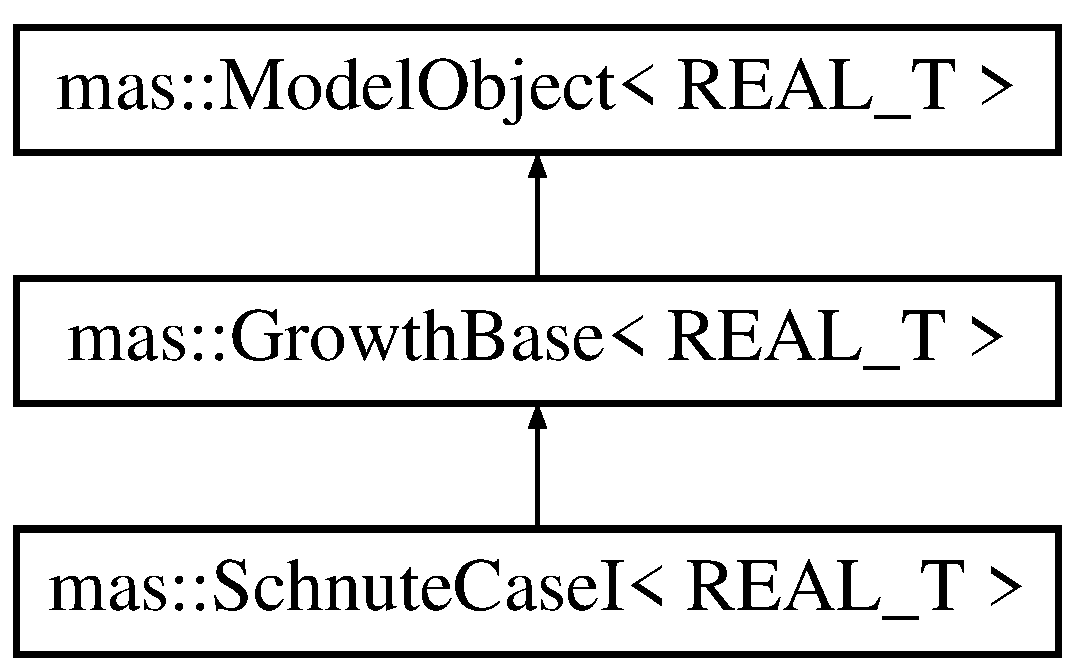
\includegraphics[height=3.000000cm]{structmas_1_1_schnute_case_i}
\end{center}
\end{figure}
\subsection*{Public Types}
\begin{DoxyCompactItemize}
\item 
typedef \hyperlink{structmas_1_1_variable_trait}{Variable\-Trait}$<$ R\-E\-A\-L\-\_\-\-T $>$\\*
\-::\hyperlink{structmas_1_1_schnute_case_i_a6655933b5cf46aabdff359c07c095a95}{variable} \hyperlink{structmas_1_1_schnute_case_i_a6655933b5cf46aabdff359c07c095a95}{variable}
\end{DoxyCompactItemize}
\subsection*{Public Member Functions}
\begin{DoxyCompactItemize}
\item 
virtual const \hyperlink{structmas_1_1_schnute_case_i_a6655933b5cf46aabdff359c07c095a95}{variable} \hyperlink{structmas_1_1_schnute_case_i_acc1a2f969120393ef5275ee3f297dfc9}{Evaluate} (const \hyperlink{structmas_1_1_schnute_case_i_a6655933b5cf46aabdff359c07c095a95}{variable} \&age, const int \&sex)
\item 
virtual const std\-::string \hyperlink{structmas_1_1_schnute_case_i_a84e734071e4bf0cce1d36c00f94768db}{To\-J\-S\-O\-N\-String} ()
\item 
virtual const std\-::string \hyperlink{structmas_1_1_schnute_case_i_a5588227ee2b536f92b34c02d95a7d148}{Name} ()
\item 
virtual std\-::string \hyperlink{structmas_1_1_schnute_case_i_a75bd8ce2e0224680c775a70122f18232}{To\-String} ()
\end{DoxyCompactItemize}
\subsection*{Public Attributes}
\begin{DoxyCompactItemize}
\item 
\hyperlink{structmas_1_1_schnute_case_i_a6655933b5cf46aabdff359c07c095a95}{variable} \hyperlink{structmas_1_1_schnute_case_i_a65872d07f8ecb249f7eecc7d167d8393}{alpha}
\item 
\hyperlink{structmas_1_1_schnute_case_i_a6655933b5cf46aabdff359c07c095a95}{variable} \hyperlink{structmas_1_1_schnute_case_i_a375472b1c6d9a60992aba819d54b4ece}{beta}
\item 
\hyperlink{structmas_1_1_schnute_case_i_a6655933b5cf46aabdff359c07c095a95}{variable} \hyperlink{structmas_1_1_schnute_case_i_a36282ecc11a1baa5c47a31d9419853a0}{lmin}
\item 
\hyperlink{structmas_1_1_schnute_case_i_a6655933b5cf46aabdff359c07c095a95}{variable} \hyperlink{structmas_1_1_schnute_case_i_ac393da368b9ab41438b697d78b700ee7}{lmax}
\end{DoxyCompactItemize}


\subsection{Detailed Description}
\subsubsection*{template$<$typename R\-E\-A\-L\-\_\-\-T$>$struct mas\-::\-Schnute\-Case\-I$<$ R\-E\-A\-L\-\_\-\-T $>$}



Definition at line 169 of file Growth.\-hpp.



\subsection{Member Typedef Documentation}
\hypertarget{structmas_1_1_schnute_case_i_a6655933b5cf46aabdff359c07c095a95}{\index{mas\-::\-Schnute\-Case\-I@{mas\-::\-Schnute\-Case\-I}!variable@{variable}}
\index{variable@{variable}!mas::SchnuteCaseI@{mas\-::\-Schnute\-Case\-I}}
\subsubsection[{variable}]{\setlength{\rightskip}{0pt plus 5cm}template$<$typename R\-E\-A\-L\-\_\-\-T $>$ typedef {\bf Variable\-Trait}$<$R\-E\-A\-L\-\_\-\-T$>$\-::{\bf variable} {\bf mas\-::\-Schnute\-Case\-I}$<$ R\-E\-A\-L\-\_\-\-T $>$\-::{\bf variable}}}\label{structmas_1_1_schnute_case_i_a6655933b5cf46aabdff359c07c095a95}


Definition at line 170 of file Growth.\-hpp.



\subsection{Member Function Documentation}
\hypertarget{structmas_1_1_schnute_case_i_acc1a2f969120393ef5275ee3f297dfc9}{\index{mas\-::\-Schnute\-Case\-I@{mas\-::\-Schnute\-Case\-I}!Evaluate@{Evaluate}}
\index{Evaluate@{Evaluate}!mas::SchnuteCaseI@{mas\-::\-Schnute\-Case\-I}}
\subsubsection[{Evaluate}]{\setlength{\rightskip}{0pt plus 5cm}template$<$typename R\-E\-A\-L\-\_\-\-T $>$ virtual const {\bf variable} {\bf mas\-::\-Schnute\-Case\-I}$<$ R\-E\-A\-L\-\_\-\-T $>$\-::Evaluate (
\begin{DoxyParamCaption}
\item[{const {\bf variable} \&}]{age, }
\item[{const int \&}]{sex}
\end{DoxyParamCaption}
)\hspace{0.3cm}{\ttfamily [inline]}, {\ttfamily [virtual]}}}\label{structmas_1_1_schnute_case_i_acc1a2f969120393ef5275ee3f297dfc9}
Computes the length of a fish at age by sex.


\begin{DoxyParams}{Parameters}
{\em age} & \\
\hline
{\em sex} & \\
\hline
\end{DoxyParams}
\begin{DoxyReturn}{Returns}
length 
\end{DoxyReturn}


Implements \hyperlink{structmas_1_1_growth_base_a381e3400e22b2739830351acdf4689b5}{mas\-::\-Growth\-Base$<$ R\-E\-A\-L\-\_\-\-T $>$}.



Definition at line 176 of file Growth.\-hpp.

\hypertarget{structmas_1_1_schnute_case_i_a5588227ee2b536f92b34c02d95a7d148}{\index{mas\-::\-Schnute\-Case\-I@{mas\-::\-Schnute\-Case\-I}!Name@{Name}}
\index{Name@{Name}!mas::SchnuteCaseI@{mas\-::\-Schnute\-Case\-I}}
\subsubsection[{Name}]{\setlength{\rightskip}{0pt plus 5cm}template$<$typename R\-E\-A\-L\-\_\-\-T $>$ virtual const std\-::string {\bf mas\-::\-Schnute\-Case\-I}$<$ R\-E\-A\-L\-\_\-\-T $>$\-::Name (
\begin{DoxyParamCaption}
{}
\end{DoxyParamCaption}
)\hspace{0.3cm}{\ttfamily [inline]}, {\ttfamily [virtual]}}}\label{structmas_1_1_schnute_case_i_a5588227ee2b536f92b34c02d95a7d148}


Reimplemented from \hyperlink{structmas_1_1_growth_base_a3645c79a5cd9ed606bcf2f381aef5259}{mas\-::\-Growth\-Base$<$ R\-E\-A\-L\-\_\-\-T $>$}.



Definition at line 205 of file Growth.\-hpp.

\hypertarget{structmas_1_1_schnute_case_i_a84e734071e4bf0cce1d36c00f94768db}{\index{mas\-::\-Schnute\-Case\-I@{mas\-::\-Schnute\-Case\-I}!To\-J\-S\-O\-N\-String@{To\-J\-S\-O\-N\-String}}
\index{To\-J\-S\-O\-N\-String@{To\-J\-S\-O\-N\-String}!mas::SchnuteCaseI@{mas\-::\-Schnute\-Case\-I}}
\subsubsection[{To\-J\-S\-O\-N\-String}]{\setlength{\rightskip}{0pt plus 5cm}template$<$typename R\-E\-A\-L\-\_\-\-T $>$ virtual const std\-::string {\bf mas\-::\-Schnute\-Case\-I}$<$ R\-E\-A\-L\-\_\-\-T $>$\-::To\-J\-S\-O\-N\-String (
\begin{DoxyParamCaption}
{}
\end{DoxyParamCaption}
)\hspace{0.3cm}{\ttfamily [inline]}, {\ttfamily [virtual]}}}\label{structmas_1_1_schnute_case_i_a84e734071e4bf0cce1d36c00f94768db}


Reimplemented from \hyperlink{structmas_1_1_model_object_af40b3c89b11919fc5aea21dcf1cd027b}{mas\-::\-Model\-Object$<$ R\-E\-A\-L\-\_\-\-T $>$}.



Definition at line 184 of file Growth.\-hpp.

\hypertarget{structmas_1_1_schnute_case_i_a75bd8ce2e0224680c775a70122f18232}{\index{mas\-::\-Schnute\-Case\-I@{mas\-::\-Schnute\-Case\-I}!To\-String@{To\-String}}
\index{To\-String@{To\-String}!mas::SchnuteCaseI@{mas\-::\-Schnute\-Case\-I}}
\subsubsection[{To\-String}]{\setlength{\rightskip}{0pt plus 5cm}template$<$typename R\-E\-A\-L\-\_\-\-T $>$ virtual std\-::string {\bf mas\-::\-Schnute\-Case\-I}$<$ R\-E\-A\-L\-\_\-\-T $>$\-::To\-String (
\begin{DoxyParamCaption}
{}
\end{DoxyParamCaption}
)\hspace{0.3cm}{\ttfamily [inline]}, {\ttfamily [virtual]}}}\label{structmas_1_1_schnute_case_i_a75bd8ce2e0224680c775a70122f18232}


Reimplemented from \hyperlink{structmas_1_1_model_object_a8eaf6c7c52e42ea8869aefa318358cb5}{mas\-::\-Model\-Object$<$ R\-E\-A\-L\-\_\-\-T $>$}.



Definition at line 209 of file Growth.\-hpp.



\subsection{Member Data Documentation}
\hypertarget{structmas_1_1_schnute_case_i_a65872d07f8ecb249f7eecc7d167d8393}{\index{mas\-::\-Schnute\-Case\-I@{mas\-::\-Schnute\-Case\-I}!alpha@{alpha}}
\index{alpha@{alpha}!mas::SchnuteCaseI@{mas\-::\-Schnute\-Case\-I}}
\subsubsection[{alpha}]{\setlength{\rightskip}{0pt plus 5cm}template$<$typename R\-E\-A\-L\-\_\-\-T $>$ {\bf variable} {\bf mas\-::\-Schnute\-Case\-I}$<$ R\-E\-A\-L\-\_\-\-T $>$\-::alpha}}\label{structmas_1_1_schnute_case_i_a65872d07f8ecb249f7eecc7d167d8393}


Definition at line 171 of file Growth.\-hpp.

\hypertarget{structmas_1_1_schnute_case_i_a375472b1c6d9a60992aba819d54b4ece}{\index{mas\-::\-Schnute\-Case\-I@{mas\-::\-Schnute\-Case\-I}!beta@{beta}}
\index{beta@{beta}!mas::SchnuteCaseI@{mas\-::\-Schnute\-Case\-I}}
\subsubsection[{beta}]{\setlength{\rightskip}{0pt plus 5cm}template$<$typename R\-E\-A\-L\-\_\-\-T $>$ {\bf variable} {\bf mas\-::\-Schnute\-Case\-I}$<$ R\-E\-A\-L\-\_\-\-T $>$\-::beta}}\label{structmas_1_1_schnute_case_i_a375472b1c6d9a60992aba819d54b4ece}


Definition at line 172 of file Growth.\-hpp.

\hypertarget{structmas_1_1_schnute_case_i_ac393da368b9ab41438b697d78b700ee7}{\index{mas\-::\-Schnute\-Case\-I@{mas\-::\-Schnute\-Case\-I}!lmax@{lmax}}
\index{lmax@{lmax}!mas::SchnuteCaseI@{mas\-::\-Schnute\-Case\-I}}
\subsubsection[{lmax}]{\setlength{\rightskip}{0pt plus 5cm}template$<$typename R\-E\-A\-L\-\_\-\-T $>$ {\bf variable} {\bf mas\-::\-Schnute\-Case\-I}$<$ R\-E\-A\-L\-\_\-\-T $>$\-::lmax}}\label{structmas_1_1_schnute_case_i_ac393da368b9ab41438b697d78b700ee7}


Definition at line 174 of file Growth.\-hpp.

\hypertarget{structmas_1_1_schnute_case_i_a36282ecc11a1baa5c47a31d9419853a0}{\index{mas\-::\-Schnute\-Case\-I@{mas\-::\-Schnute\-Case\-I}!lmin@{lmin}}
\index{lmin@{lmin}!mas::SchnuteCaseI@{mas\-::\-Schnute\-Case\-I}}
\subsubsection[{lmin}]{\setlength{\rightskip}{0pt plus 5cm}template$<$typename R\-E\-A\-L\-\_\-\-T $>$ {\bf variable} {\bf mas\-::\-Schnute\-Case\-I}$<$ R\-E\-A\-L\-\_\-\-T $>$\-::lmin}}\label{structmas_1_1_schnute_case_i_a36282ecc11a1baa5c47a31d9419853a0}


Definition at line 173 of file Growth.\-hpp.



The documentation for this struct was generated from the following file\-:\begin{DoxyCompactItemize}
\item 
/home/oppy/\-Net\-Beans\-Projects/mas/\hyperlink{_growth_8hpp}{Growth.\-hpp}\end{DoxyCompactItemize}

\hypertarget{structmas_1_1_schnute_case_i_i}{\section{mas\-:\-:Schnute\-Case\-I\-I$<$ R\-E\-A\-L\-\_\-\-T $>$ Struct Template Reference}
\label{structmas_1_1_schnute_case_i_i}\index{mas\-::\-Schnute\-Case\-I\-I$<$ R\-E\-A\-L\-\_\-\-T $>$@{mas\-::\-Schnute\-Case\-I\-I$<$ R\-E\-A\-L\-\_\-\-T $>$}}
}


{\ttfamily \#include $<$Growth.\-hpp$>$}

Inheritance diagram for mas\-:\-:Schnute\-Case\-I\-I$<$ R\-E\-A\-L\-\_\-\-T $>$\-:\begin{figure}[H]
\begin{center}
\leavevmode
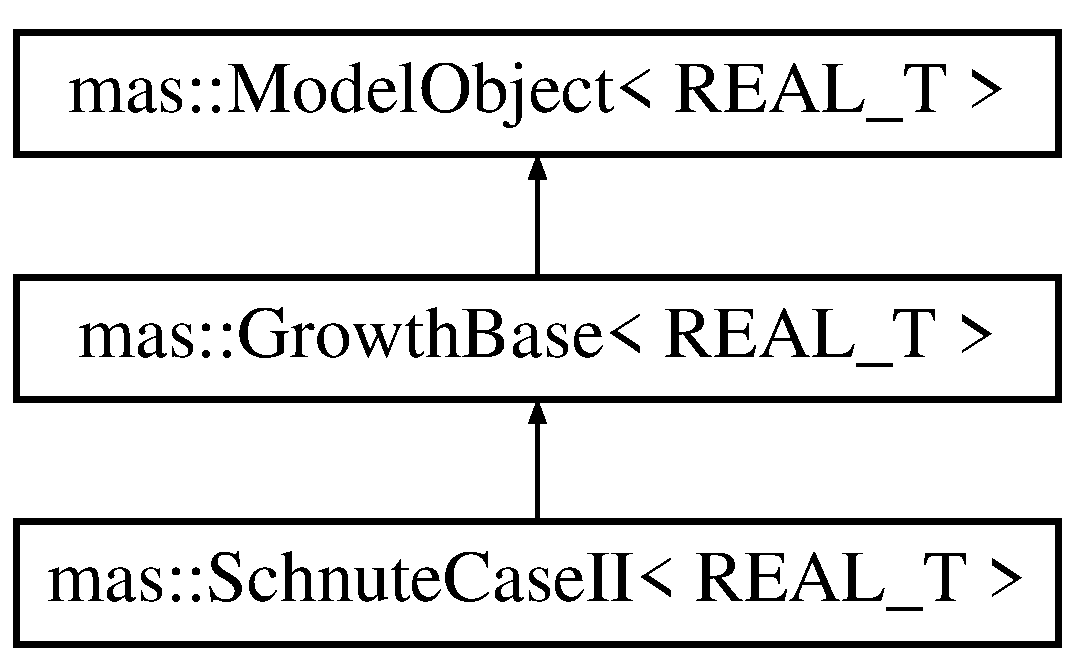
\includegraphics[height=3.000000cm]{structmas_1_1_schnute_case_i_i}
\end{center}
\end{figure}
\subsection*{Public Types}
\begin{DoxyCompactItemize}
\item 
typedef \hyperlink{structmas_1_1_variable_trait}{Variable\-Trait}$<$ R\-E\-A\-L\-\_\-\-T $>$\\*
\-::\hyperlink{structmas_1_1_schnute_case_i_i_a44a5def50d599f85b1c0fbe1b44f139b}{variable} \hyperlink{structmas_1_1_schnute_case_i_i_a44a5def50d599f85b1c0fbe1b44f139b}{variable}
\end{DoxyCompactItemize}
\subsection*{Public Member Functions}
\begin{DoxyCompactItemize}
\item 
virtual const \hyperlink{structmas_1_1_schnute_case_i_i_a44a5def50d599f85b1c0fbe1b44f139b}{variable} \hyperlink{structmas_1_1_schnute_case_i_i_ac582befc654cf955f0afafed8889b0e1}{Evaluate} (const \hyperlink{structmas_1_1_schnute_case_i_i_a44a5def50d599f85b1c0fbe1b44f139b}{variable} \&age, const int \&sex)
\item 
virtual const std\-::string \hyperlink{structmas_1_1_schnute_case_i_i_a291cd832a760d0a08e838fd251f98b2b}{To\-J\-S\-O\-N\-String} ()
\item 
virtual const std\-::string \hyperlink{structmas_1_1_schnute_case_i_i_a1f2900afe54ea24bcd555dd5eab8ce03}{Name} ()
\item 
virtual std\-::string \hyperlink{structmas_1_1_schnute_case_i_i_ac4cca4d5d808023e1a72651ea090fc58}{To\-String} ()
\end{DoxyCompactItemize}
\subsection*{Public Attributes}
\begin{DoxyCompactItemize}
\item 
\hyperlink{structmas_1_1_schnute_case_i_i_a44a5def50d599f85b1c0fbe1b44f139b}{variable} \hyperlink{structmas_1_1_schnute_case_i_i_aab10fd7b8522029960059666e872c461}{alpha}
\item 
\hyperlink{structmas_1_1_schnute_case_i_i_a44a5def50d599f85b1c0fbe1b44f139b}{variable} \hyperlink{structmas_1_1_schnute_case_i_i_ab7ff973aeb99b0e7f714ba5bdefcba10}{lmin}
\item 
\hyperlink{structmas_1_1_schnute_case_i_i_a44a5def50d599f85b1c0fbe1b44f139b}{variable} \hyperlink{structmas_1_1_schnute_case_i_i_a2f33253a32b5b0680cbacfa1f5e29f64}{lmax}
\end{DoxyCompactItemize}


\subsection{Detailed Description}
\subsubsection*{template$<$typename R\-E\-A\-L\-\_\-\-T$>$struct mas\-::\-Schnute\-Case\-I\-I$<$ R\-E\-A\-L\-\_\-\-T $>$}



Definition at line 221 of file Growth.\-hpp.



\subsection{Member Typedef Documentation}
\hypertarget{structmas_1_1_schnute_case_i_i_a44a5def50d599f85b1c0fbe1b44f139b}{\index{mas\-::\-Schnute\-Case\-I\-I@{mas\-::\-Schnute\-Case\-I\-I}!variable@{variable}}
\index{variable@{variable}!mas::SchnuteCaseII@{mas\-::\-Schnute\-Case\-I\-I}}
\subsubsection[{variable}]{\setlength{\rightskip}{0pt plus 5cm}template$<$typename R\-E\-A\-L\-\_\-\-T $>$ typedef {\bf Variable\-Trait}$<$R\-E\-A\-L\-\_\-\-T$>$\-::{\bf variable} {\bf mas\-::\-Schnute\-Case\-I\-I}$<$ R\-E\-A\-L\-\_\-\-T $>$\-::{\bf variable}}}\label{structmas_1_1_schnute_case_i_i_a44a5def50d599f85b1c0fbe1b44f139b}


Definition at line 222 of file Growth.\-hpp.



\subsection{Member Function Documentation}
\hypertarget{structmas_1_1_schnute_case_i_i_ac582befc654cf955f0afafed8889b0e1}{\index{mas\-::\-Schnute\-Case\-I\-I@{mas\-::\-Schnute\-Case\-I\-I}!Evaluate@{Evaluate}}
\index{Evaluate@{Evaluate}!mas::SchnuteCaseII@{mas\-::\-Schnute\-Case\-I\-I}}
\subsubsection[{Evaluate}]{\setlength{\rightskip}{0pt plus 5cm}template$<$typename R\-E\-A\-L\-\_\-\-T $>$ virtual const {\bf variable} {\bf mas\-::\-Schnute\-Case\-I\-I}$<$ R\-E\-A\-L\-\_\-\-T $>$\-::Evaluate (
\begin{DoxyParamCaption}
\item[{const {\bf variable} \&}]{age, }
\item[{const int \&}]{sex}
\end{DoxyParamCaption}
)\hspace{0.3cm}{\ttfamily [inline]}, {\ttfamily [virtual]}}}\label{structmas_1_1_schnute_case_i_i_ac582befc654cf955f0afafed8889b0e1}
Computes the length of a fish at age by sex.


\begin{DoxyParams}{Parameters}
{\em age} & \\
\hline
{\em sex} & \\
\hline
\end{DoxyParams}
\begin{DoxyReturn}{Returns}
length 
\end{DoxyReturn}


Implements \hyperlink{structmas_1_1_growth_base_a381e3400e22b2739830351acdf4689b5}{mas\-::\-Growth\-Base$<$ R\-E\-A\-L\-\_\-\-T $>$}.



Definition at line 227 of file Growth.\-hpp.

\hypertarget{structmas_1_1_schnute_case_i_i_a1f2900afe54ea24bcd555dd5eab8ce03}{\index{mas\-::\-Schnute\-Case\-I\-I@{mas\-::\-Schnute\-Case\-I\-I}!Name@{Name}}
\index{Name@{Name}!mas::SchnuteCaseII@{mas\-::\-Schnute\-Case\-I\-I}}
\subsubsection[{Name}]{\setlength{\rightskip}{0pt plus 5cm}template$<$typename R\-E\-A\-L\-\_\-\-T $>$ virtual const std\-::string {\bf mas\-::\-Schnute\-Case\-I\-I}$<$ R\-E\-A\-L\-\_\-\-T $>$\-::Name (
\begin{DoxyParamCaption}
{}
\end{DoxyParamCaption}
)\hspace{0.3cm}{\ttfamily [inline]}, {\ttfamily [virtual]}}}\label{structmas_1_1_schnute_case_i_i_a1f2900afe54ea24bcd555dd5eab8ce03}


Reimplemented from \hyperlink{structmas_1_1_growth_base_a3645c79a5cd9ed606bcf2f381aef5259}{mas\-::\-Growth\-Base$<$ R\-E\-A\-L\-\_\-\-T $>$}.



Definition at line 254 of file Growth.\-hpp.

\hypertarget{structmas_1_1_schnute_case_i_i_a291cd832a760d0a08e838fd251f98b2b}{\index{mas\-::\-Schnute\-Case\-I\-I@{mas\-::\-Schnute\-Case\-I\-I}!To\-J\-S\-O\-N\-String@{To\-J\-S\-O\-N\-String}}
\index{To\-J\-S\-O\-N\-String@{To\-J\-S\-O\-N\-String}!mas::SchnuteCaseII@{mas\-::\-Schnute\-Case\-I\-I}}
\subsubsection[{To\-J\-S\-O\-N\-String}]{\setlength{\rightskip}{0pt plus 5cm}template$<$typename R\-E\-A\-L\-\_\-\-T $>$ virtual const std\-::string {\bf mas\-::\-Schnute\-Case\-I\-I}$<$ R\-E\-A\-L\-\_\-\-T $>$\-::To\-J\-S\-O\-N\-String (
\begin{DoxyParamCaption}
{}
\end{DoxyParamCaption}
)\hspace{0.3cm}{\ttfamily [inline]}, {\ttfamily [virtual]}}}\label{structmas_1_1_schnute_case_i_i_a291cd832a760d0a08e838fd251f98b2b}


Reimplemented from \hyperlink{structmas_1_1_model_object_af40b3c89b11919fc5aea21dcf1cd027b}{mas\-::\-Model\-Object$<$ R\-E\-A\-L\-\_\-\-T $>$}.



Definition at line 234 of file Growth.\-hpp.

\hypertarget{structmas_1_1_schnute_case_i_i_ac4cca4d5d808023e1a72651ea090fc58}{\index{mas\-::\-Schnute\-Case\-I\-I@{mas\-::\-Schnute\-Case\-I\-I}!To\-String@{To\-String}}
\index{To\-String@{To\-String}!mas::SchnuteCaseII@{mas\-::\-Schnute\-Case\-I\-I}}
\subsubsection[{To\-String}]{\setlength{\rightskip}{0pt plus 5cm}template$<$typename R\-E\-A\-L\-\_\-\-T $>$ virtual std\-::string {\bf mas\-::\-Schnute\-Case\-I\-I}$<$ R\-E\-A\-L\-\_\-\-T $>$\-::To\-String (
\begin{DoxyParamCaption}
{}
\end{DoxyParamCaption}
)\hspace{0.3cm}{\ttfamily [inline]}, {\ttfamily [virtual]}}}\label{structmas_1_1_schnute_case_i_i_ac4cca4d5d808023e1a72651ea090fc58}


Reimplemented from \hyperlink{structmas_1_1_model_object_a8eaf6c7c52e42ea8869aefa318358cb5}{mas\-::\-Model\-Object$<$ R\-E\-A\-L\-\_\-\-T $>$}.



Definition at line 258 of file Growth.\-hpp.



\subsection{Member Data Documentation}
\hypertarget{structmas_1_1_schnute_case_i_i_aab10fd7b8522029960059666e872c461}{\index{mas\-::\-Schnute\-Case\-I\-I@{mas\-::\-Schnute\-Case\-I\-I}!alpha@{alpha}}
\index{alpha@{alpha}!mas::SchnuteCaseII@{mas\-::\-Schnute\-Case\-I\-I}}
\subsubsection[{alpha}]{\setlength{\rightskip}{0pt plus 5cm}template$<$typename R\-E\-A\-L\-\_\-\-T $>$ {\bf variable} {\bf mas\-::\-Schnute\-Case\-I\-I}$<$ R\-E\-A\-L\-\_\-\-T $>$\-::alpha}}\label{structmas_1_1_schnute_case_i_i_aab10fd7b8522029960059666e872c461}


Definition at line 223 of file Growth.\-hpp.

\hypertarget{structmas_1_1_schnute_case_i_i_a2f33253a32b5b0680cbacfa1f5e29f64}{\index{mas\-::\-Schnute\-Case\-I\-I@{mas\-::\-Schnute\-Case\-I\-I}!lmax@{lmax}}
\index{lmax@{lmax}!mas::SchnuteCaseII@{mas\-::\-Schnute\-Case\-I\-I}}
\subsubsection[{lmax}]{\setlength{\rightskip}{0pt plus 5cm}template$<$typename R\-E\-A\-L\-\_\-\-T $>$ {\bf variable} {\bf mas\-::\-Schnute\-Case\-I\-I}$<$ R\-E\-A\-L\-\_\-\-T $>$\-::lmax}}\label{structmas_1_1_schnute_case_i_i_a2f33253a32b5b0680cbacfa1f5e29f64}


Definition at line 225 of file Growth.\-hpp.

\hypertarget{structmas_1_1_schnute_case_i_i_ab7ff973aeb99b0e7f714ba5bdefcba10}{\index{mas\-::\-Schnute\-Case\-I\-I@{mas\-::\-Schnute\-Case\-I\-I}!lmin@{lmin}}
\index{lmin@{lmin}!mas::SchnuteCaseII@{mas\-::\-Schnute\-Case\-I\-I}}
\subsubsection[{lmin}]{\setlength{\rightskip}{0pt plus 5cm}template$<$typename R\-E\-A\-L\-\_\-\-T $>$ {\bf variable} {\bf mas\-::\-Schnute\-Case\-I\-I}$<$ R\-E\-A\-L\-\_\-\-T $>$\-::lmin}}\label{structmas_1_1_schnute_case_i_i_ab7ff973aeb99b0e7f714ba5bdefcba10}


Definition at line 224 of file Growth.\-hpp.



The documentation for this struct was generated from the following file\-:\begin{DoxyCompactItemize}
\item 
/home/oppy/\-Net\-Beans\-Projects/mas/\hyperlink{_growth_8hpp}{Growth.\-hpp}\end{DoxyCompactItemize}

\hypertarget{structmas_1_1_schnute_case_i_i_i}{\section{mas\-:\-:Schnute\-Case\-I\-I\-I$<$ R\-E\-A\-L\-\_\-\-T $>$ Struct Template Reference}
\label{structmas_1_1_schnute_case_i_i_i}\index{mas\-::\-Schnute\-Case\-I\-I\-I$<$ R\-E\-A\-L\-\_\-\-T $>$@{mas\-::\-Schnute\-Case\-I\-I\-I$<$ R\-E\-A\-L\-\_\-\-T $>$}}
}


{\ttfamily \#include $<$Growth.\-hpp$>$}

Inheritance diagram for mas\-:\-:Schnute\-Case\-I\-I\-I$<$ R\-E\-A\-L\-\_\-\-T $>$\-:\begin{figure}[H]
\begin{center}
\leavevmode
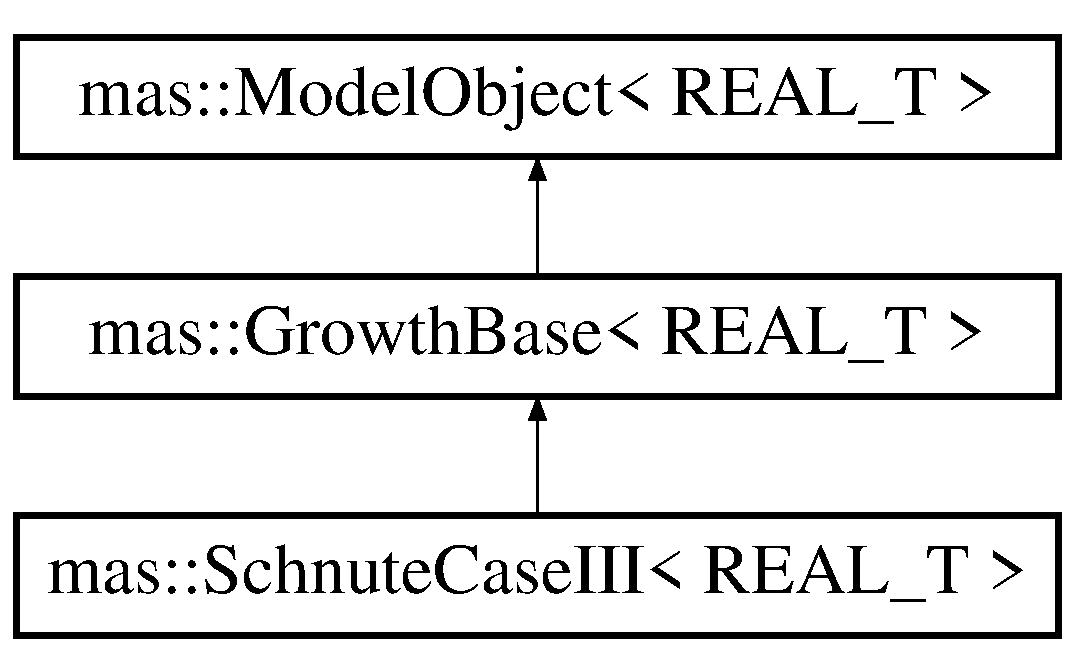
\includegraphics[height=3.000000cm]{structmas_1_1_schnute_case_i_i_i}
\end{center}
\end{figure}
\subsection*{Public Types}
\begin{DoxyCompactItemize}
\item 
typedef \hyperlink{structmas_1_1_variable_trait}{Variable\-Trait}$<$ R\-E\-A\-L\-\_\-\-T $>$\\*
\-::\hyperlink{structmas_1_1_schnute_case_i_i_i_a47b89c3219bc40a67dcb3dd626a585fa}{variable} \hyperlink{structmas_1_1_schnute_case_i_i_i_a47b89c3219bc40a67dcb3dd626a585fa}{variable}
\end{DoxyCompactItemize}
\subsection*{Public Member Functions}
\begin{DoxyCompactItemize}
\item 
virtual const \hyperlink{structmas_1_1_schnute_case_i_i_i_a47b89c3219bc40a67dcb3dd626a585fa}{variable} \hyperlink{structmas_1_1_schnute_case_i_i_i_a36829dacc125f07c7c9595f1e8ca0d8a}{Evaluate} (const \hyperlink{structmas_1_1_schnute_case_i_i_i_a47b89c3219bc40a67dcb3dd626a585fa}{variable} \&age, const int \&sex)
\item 
virtual const std\-::string \hyperlink{structmas_1_1_schnute_case_i_i_i_a7f55a0a6f9f4f8f577c952ec974c89c4}{To\-J\-S\-O\-N\-String} ()
\item 
virtual const std\-::string \hyperlink{structmas_1_1_schnute_case_i_i_i_a0b7e35620fbbdc033702c304054aa9e3}{Name} ()
\item 
virtual std\-::string \hyperlink{structmas_1_1_schnute_case_i_i_i_af99d1855589bc44641952cfc89d11a72}{To\-String} ()
\end{DoxyCompactItemize}
\subsection*{Public Attributes}
\begin{DoxyCompactItemize}
\item 
\hyperlink{structmas_1_1_schnute_case_i_i_i_a47b89c3219bc40a67dcb3dd626a585fa}{variable} \hyperlink{structmas_1_1_schnute_case_i_i_i_a327d0f288525e7f5c531876245728dcf}{alpha}
\item 
\hyperlink{structmas_1_1_schnute_case_i_i_i_a47b89c3219bc40a67dcb3dd626a585fa}{variable} \hyperlink{structmas_1_1_schnute_case_i_i_i_a857518ba684261d8b0a7bdd08e2c48c3}{beta}
\item 
\hyperlink{structmas_1_1_schnute_case_i_i_i_a47b89c3219bc40a67dcb3dd626a585fa}{variable} \hyperlink{structmas_1_1_schnute_case_i_i_i_a428c1da272df27ab99d278aef25fdb9d}{lmin}
\item 
\hyperlink{structmas_1_1_schnute_case_i_i_i_a47b89c3219bc40a67dcb3dd626a585fa}{variable} \hyperlink{structmas_1_1_schnute_case_i_i_i_a4129bd8069255252549453d2ec3fefb7}{lmax}
\end{DoxyCompactItemize}


\subsection{Detailed Description}
\subsubsection*{template$<$typename R\-E\-A\-L\-\_\-\-T$>$struct mas\-::\-Schnute\-Case\-I\-I\-I$<$ R\-E\-A\-L\-\_\-\-T $>$}



Definition at line 269 of file Growth.\-hpp.



\subsection{Member Typedef Documentation}
\hypertarget{structmas_1_1_schnute_case_i_i_i_a47b89c3219bc40a67dcb3dd626a585fa}{\index{mas\-::\-Schnute\-Case\-I\-I\-I@{mas\-::\-Schnute\-Case\-I\-I\-I}!variable@{variable}}
\index{variable@{variable}!mas::SchnuteCaseIII@{mas\-::\-Schnute\-Case\-I\-I\-I}}
\subsubsection[{variable}]{\setlength{\rightskip}{0pt plus 5cm}template$<$typename R\-E\-A\-L\-\_\-\-T $>$ typedef {\bf Variable\-Trait}$<$R\-E\-A\-L\-\_\-\-T$>$\-::{\bf variable} {\bf mas\-::\-Schnute\-Case\-I\-I\-I}$<$ R\-E\-A\-L\-\_\-\-T $>$\-::{\bf variable}}}\label{structmas_1_1_schnute_case_i_i_i_a47b89c3219bc40a67dcb3dd626a585fa}


Definition at line 270 of file Growth.\-hpp.



\subsection{Member Function Documentation}
\hypertarget{structmas_1_1_schnute_case_i_i_i_a36829dacc125f07c7c9595f1e8ca0d8a}{\index{mas\-::\-Schnute\-Case\-I\-I\-I@{mas\-::\-Schnute\-Case\-I\-I\-I}!Evaluate@{Evaluate}}
\index{Evaluate@{Evaluate}!mas::SchnuteCaseIII@{mas\-::\-Schnute\-Case\-I\-I\-I}}
\subsubsection[{Evaluate}]{\setlength{\rightskip}{0pt plus 5cm}template$<$typename R\-E\-A\-L\-\_\-\-T $>$ virtual const {\bf variable} {\bf mas\-::\-Schnute\-Case\-I\-I\-I}$<$ R\-E\-A\-L\-\_\-\-T $>$\-::Evaluate (
\begin{DoxyParamCaption}
\item[{const {\bf variable} \&}]{age, }
\item[{const int \&}]{sex}
\end{DoxyParamCaption}
)\hspace{0.3cm}{\ttfamily [inline]}, {\ttfamily [virtual]}}}\label{structmas_1_1_schnute_case_i_i_i_a36829dacc125f07c7c9595f1e8ca0d8a}
Computes the length of a fish at age by sex.


\begin{DoxyParams}{Parameters}
{\em age} & \\
\hline
{\em sex} & \\
\hline
\end{DoxyParams}
\begin{DoxyReturn}{Returns}
length 
\end{DoxyReturn}


Implements \hyperlink{structmas_1_1_growth_base_a381e3400e22b2739830351acdf4689b5}{mas\-::\-Growth\-Base$<$ R\-E\-A\-L\-\_\-\-T $>$}.



Definition at line 276 of file Growth.\-hpp.

\hypertarget{structmas_1_1_schnute_case_i_i_i_a0b7e35620fbbdc033702c304054aa9e3}{\index{mas\-::\-Schnute\-Case\-I\-I\-I@{mas\-::\-Schnute\-Case\-I\-I\-I}!Name@{Name}}
\index{Name@{Name}!mas::SchnuteCaseIII@{mas\-::\-Schnute\-Case\-I\-I\-I}}
\subsubsection[{Name}]{\setlength{\rightskip}{0pt plus 5cm}template$<$typename R\-E\-A\-L\-\_\-\-T $>$ virtual const std\-::string {\bf mas\-::\-Schnute\-Case\-I\-I\-I}$<$ R\-E\-A\-L\-\_\-\-T $>$\-::Name (
\begin{DoxyParamCaption}
{}
\end{DoxyParamCaption}
)\hspace{0.3cm}{\ttfamily [inline]}, {\ttfamily [virtual]}}}\label{structmas_1_1_schnute_case_i_i_i_a0b7e35620fbbdc033702c304054aa9e3}


Reimplemented from \hyperlink{structmas_1_1_growth_base_a3645c79a5cd9ed606bcf2f381aef5259}{mas\-::\-Growth\-Base$<$ R\-E\-A\-L\-\_\-\-T $>$}.



Definition at line 306 of file Growth.\-hpp.

\hypertarget{structmas_1_1_schnute_case_i_i_i_a7f55a0a6f9f4f8f577c952ec974c89c4}{\index{mas\-::\-Schnute\-Case\-I\-I\-I@{mas\-::\-Schnute\-Case\-I\-I\-I}!To\-J\-S\-O\-N\-String@{To\-J\-S\-O\-N\-String}}
\index{To\-J\-S\-O\-N\-String@{To\-J\-S\-O\-N\-String}!mas::SchnuteCaseIII@{mas\-::\-Schnute\-Case\-I\-I\-I}}
\subsubsection[{To\-J\-S\-O\-N\-String}]{\setlength{\rightskip}{0pt plus 5cm}template$<$typename R\-E\-A\-L\-\_\-\-T $>$ virtual const std\-::string {\bf mas\-::\-Schnute\-Case\-I\-I\-I}$<$ R\-E\-A\-L\-\_\-\-T $>$\-::To\-J\-S\-O\-N\-String (
\begin{DoxyParamCaption}
{}
\end{DoxyParamCaption}
)\hspace{0.3cm}{\ttfamily [inline]}, {\ttfamily [virtual]}}}\label{structmas_1_1_schnute_case_i_i_i_a7f55a0a6f9f4f8f577c952ec974c89c4}


Reimplemented from \hyperlink{structmas_1_1_model_object_af40b3c89b11919fc5aea21dcf1cd027b}{mas\-::\-Model\-Object$<$ R\-E\-A\-L\-\_\-\-T $>$}.



Definition at line 284 of file Growth.\-hpp.

\hypertarget{structmas_1_1_schnute_case_i_i_i_af99d1855589bc44641952cfc89d11a72}{\index{mas\-::\-Schnute\-Case\-I\-I\-I@{mas\-::\-Schnute\-Case\-I\-I\-I}!To\-String@{To\-String}}
\index{To\-String@{To\-String}!mas::SchnuteCaseIII@{mas\-::\-Schnute\-Case\-I\-I\-I}}
\subsubsection[{To\-String}]{\setlength{\rightskip}{0pt plus 5cm}template$<$typename R\-E\-A\-L\-\_\-\-T $>$ virtual std\-::string {\bf mas\-::\-Schnute\-Case\-I\-I\-I}$<$ R\-E\-A\-L\-\_\-\-T $>$\-::To\-String (
\begin{DoxyParamCaption}
{}
\end{DoxyParamCaption}
)\hspace{0.3cm}{\ttfamily [inline]}, {\ttfamily [virtual]}}}\label{structmas_1_1_schnute_case_i_i_i_af99d1855589bc44641952cfc89d11a72}


Reimplemented from \hyperlink{structmas_1_1_model_object_a8eaf6c7c52e42ea8869aefa318358cb5}{mas\-::\-Model\-Object$<$ R\-E\-A\-L\-\_\-\-T $>$}.



Definition at line 310 of file Growth.\-hpp.



\subsection{Member Data Documentation}
\hypertarget{structmas_1_1_schnute_case_i_i_i_a327d0f288525e7f5c531876245728dcf}{\index{mas\-::\-Schnute\-Case\-I\-I\-I@{mas\-::\-Schnute\-Case\-I\-I\-I}!alpha@{alpha}}
\index{alpha@{alpha}!mas::SchnuteCaseIII@{mas\-::\-Schnute\-Case\-I\-I\-I}}
\subsubsection[{alpha}]{\setlength{\rightskip}{0pt plus 5cm}template$<$typename R\-E\-A\-L\-\_\-\-T $>$ {\bf variable} {\bf mas\-::\-Schnute\-Case\-I\-I\-I}$<$ R\-E\-A\-L\-\_\-\-T $>$\-::alpha}}\label{structmas_1_1_schnute_case_i_i_i_a327d0f288525e7f5c531876245728dcf}


Definition at line 271 of file Growth.\-hpp.

\hypertarget{structmas_1_1_schnute_case_i_i_i_a857518ba684261d8b0a7bdd08e2c48c3}{\index{mas\-::\-Schnute\-Case\-I\-I\-I@{mas\-::\-Schnute\-Case\-I\-I\-I}!beta@{beta}}
\index{beta@{beta}!mas::SchnuteCaseIII@{mas\-::\-Schnute\-Case\-I\-I\-I}}
\subsubsection[{beta}]{\setlength{\rightskip}{0pt plus 5cm}template$<$typename R\-E\-A\-L\-\_\-\-T $>$ {\bf variable} {\bf mas\-::\-Schnute\-Case\-I\-I\-I}$<$ R\-E\-A\-L\-\_\-\-T $>$\-::beta}}\label{structmas_1_1_schnute_case_i_i_i_a857518ba684261d8b0a7bdd08e2c48c3}


Definition at line 272 of file Growth.\-hpp.

\hypertarget{structmas_1_1_schnute_case_i_i_i_a4129bd8069255252549453d2ec3fefb7}{\index{mas\-::\-Schnute\-Case\-I\-I\-I@{mas\-::\-Schnute\-Case\-I\-I\-I}!lmax@{lmax}}
\index{lmax@{lmax}!mas::SchnuteCaseIII@{mas\-::\-Schnute\-Case\-I\-I\-I}}
\subsubsection[{lmax}]{\setlength{\rightskip}{0pt plus 5cm}template$<$typename R\-E\-A\-L\-\_\-\-T $>$ {\bf variable} {\bf mas\-::\-Schnute\-Case\-I\-I\-I}$<$ R\-E\-A\-L\-\_\-\-T $>$\-::lmax}}\label{structmas_1_1_schnute_case_i_i_i_a4129bd8069255252549453d2ec3fefb7}


Definition at line 274 of file Growth.\-hpp.

\hypertarget{structmas_1_1_schnute_case_i_i_i_a428c1da272df27ab99d278aef25fdb9d}{\index{mas\-::\-Schnute\-Case\-I\-I\-I@{mas\-::\-Schnute\-Case\-I\-I\-I}!lmin@{lmin}}
\index{lmin@{lmin}!mas::SchnuteCaseIII@{mas\-::\-Schnute\-Case\-I\-I\-I}}
\subsubsection[{lmin}]{\setlength{\rightskip}{0pt plus 5cm}template$<$typename R\-E\-A\-L\-\_\-\-T $>$ {\bf variable} {\bf mas\-::\-Schnute\-Case\-I\-I\-I}$<$ R\-E\-A\-L\-\_\-\-T $>$\-::lmin}}\label{structmas_1_1_schnute_case_i_i_i_a428c1da272df27ab99d278aef25fdb9d}


Definition at line 273 of file Growth.\-hpp.



The documentation for this struct was generated from the following file\-:\begin{DoxyCompactItemize}
\item 
/home/oppy/\-Net\-Beans\-Projects/mas/\hyperlink{_growth_8hpp}{Growth.\-hpp}\end{DoxyCompactItemize}

\hypertarget{structmas_1_1_schnute_case_i_v}{\section{mas\-:\-:Schnute\-Case\-I\-V$<$ R\-E\-A\-L\-\_\-\-T $>$ Struct Template Reference}
\label{structmas_1_1_schnute_case_i_v}\index{mas\-::\-Schnute\-Case\-I\-V$<$ R\-E\-A\-L\-\_\-\-T $>$@{mas\-::\-Schnute\-Case\-I\-V$<$ R\-E\-A\-L\-\_\-\-T $>$}}
}


{\ttfamily \#include $<$Growth.\-hpp$>$}

Inheritance diagram for mas\-:\-:Schnute\-Case\-I\-V$<$ R\-E\-A\-L\-\_\-\-T $>$\-:\begin{figure}[H]
\begin{center}
\leavevmode
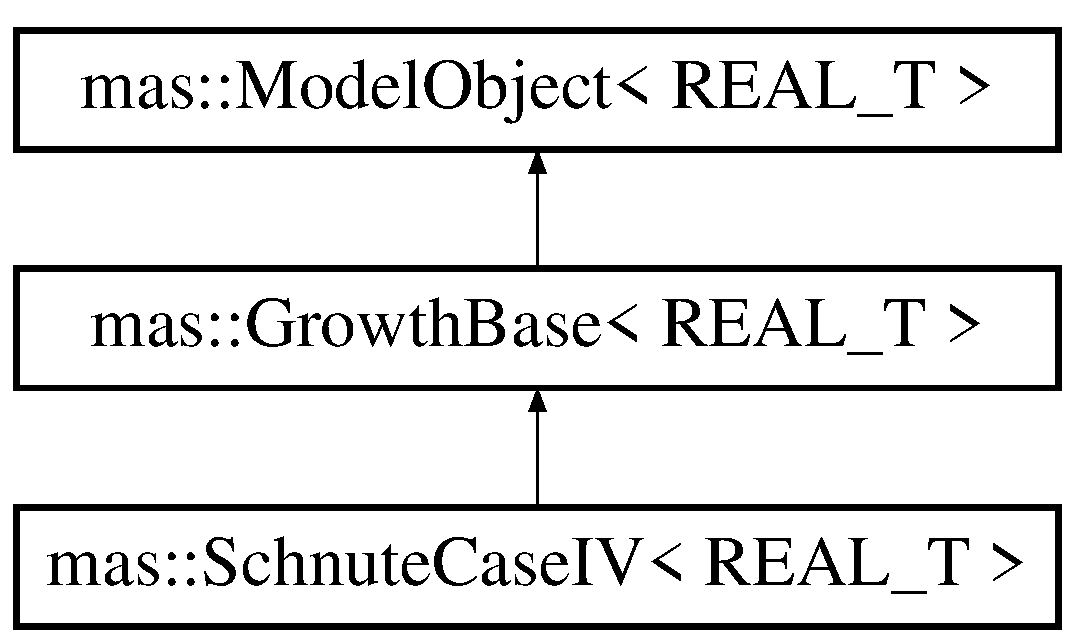
\includegraphics[height=3.000000cm]{structmas_1_1_schnute_case_i_v}
\end{center}
\end{figure}
\subsection*{Public Types}
\begin{DoxyCompactItemize}
\item 
typedef \hyperlink{structmas_1_1_variable_trait}{Variable\-Trait}$<$ R\-E\-A\-L\-\_\-\-T $>$\\*
\-::\hyperlink{structmas_1_1_schnute_case_i_v_a80605d34c604eedf01a096cefbd776a5}{variable} \hyperlink{structmas_1_1_schnute_case_i_v_a80605d34c604eedf01a096cefbd776a5}{variable}
\end{DoxyCompactItemize}
\subsection*{Public Member Functions}
\begin{DoxyCompactItemize}
\item 
virtual const \hyperlink{structmas_1_1_schnute_case_i_v_a80605d34c604eedf01a096cefbd776a5}{variable} \hyperlink{structmas_1_1_schnute_case_i_v_a8100c63161dead550bf517365e355fec}{Evaluate} (const \hyperlink{structmas_1_1_schnute_case_i_v_a80605d34c604eedf01a096cefbd776a5}{variable} \&age, const int \&sex)
\item 
virtual const std\-::string \hyperlink{structmas_1_1_schnute_case_i_v_a1f6dc0866ead488d7258b75193305c9b}{To\-J\-S\-O\-N\-String} ()
\item 
virtual const std\-::string \hyperlink{structmas_1_1_schnute_case_i_v_a7193145ce124fd855fc7d950a936fc20}{Name} ()
\item 
virtual std\-::string \hyperlink{structmas_1_1_schnute_case_i_v_ac95b913d4a28421b37e8c91e76906f2d}{To\-String} ()
\end{DoxyCompactItemize}
\subsection*{Public Attributes}
\begin{DoxyCompactItemize}
\item 
\hyperlink{structmas_1_1_schnute_case_i_v_a80605d34c604eedf01a096cefbd776a5}{variable} \hyperlink{structmas_1_1_schnute_case_i_v_a1ff44a6bb870b3ba1d553b5a4d17bd39}{alpha}
\item 
\hyperlink{structmas_1_1_schnute_case_i_v_a80605d34c604eedf01a096cefbd776a5}{variable} \hyperlink{structmas_1_1_schnute_case_i_v_a11a7d5e338909eca6126bd1384a5b0b5}{beta}
\item 
\hyperlink{structmas_1_1_schnute_case_i_v_a80605d34c604eedf01a096cefbd776a5}{variable} \hyperlink{structmas_1_1_schnute_case_i_v_a7b4d5a4e32071d80cd213ca5191bd7b1}{lmin}
\item 
\hyperlink{structmas_1_1_schnute_case_i_v_a80605d34c604eedf01a096cefbd776a5}{variable} \hyperlink{structmas_1_1_schnute_case_i_v_afadfbcde5becffb86f6049bbd59ef09c}{lmax}
\end{DoxyCompactItemize}


\subsection{Detailed Description}
\subsubsection*{template$<$typename R\-E\-A\-L\-\_\-\-T$>$struct mas\-::\-Schnute\-Case\-I\-V$<$ R\-E\-A\-L\-\_\-\-T $>$}



Definition at line 322 of file Growth.\-hpp.



\subsection{Member Typedef Documentation}
\hypertarget{structmas_1_1_schnute_case_i_v_a80605d34c604eedf01a096cefbd776a5}{\index{mas\-::\-Schnute\-Case\-I\-V@{mas\-::\-Schnute\-Case\-I\-V}!variable@{variable}}
\index{variable@{variable}!mas::SchnuteCaseIV@{mas\-::\-Schnute\-Case\-I\-V}}
\subsubsection[{variable}]{\setlength{\rightskip}{0pt plus 5cm}template$<$typename R\-E\-A\-L\-\_\-\-T $>$ typedef {\bf Variable\-Trait}$<$R\-E\-A\-L\-\_\-\-T$>$\-::{\bf variable} {\bf mas\-::\-Schnute\-Case\-I\-V}$<$ R\-E\-A\-L\-\_\-\-T $>$\-::{\bf variable}}}\label{structmas_1_1_schnute_case_i_v_a80605d34c604eedf01a096cefbd776a5}


Definition at line 323 of file Growth.\-hpp.



\subsection{Member Function Documentation}
\hypertarget{structmas_1_1_schnute_case_i_v_a8100c63161dead550bf517365e355fec}{\index{mas\-::\-Schnute\-Case\-I\-V@{mas\-::\-Schnute\-Case\-I\-V}!Evaluate@{Evaluate}}
\index{Evaluate@{Evaluate}!mas::SchnuteCaseIV@{mas\-::\-Schnute\-Case\-I\-V}}
\subsubsection[{Evaluate}]{\setlength{\rightskip}{0pt plus 5cm}template$<$typename R\-E\-A\-L\-\_\-\-T $>$ virtual const {\bf variable} {\bf mas\-::\-Schnute\-Case\-I\-V}$<$ R\-E\-A\-L\-\_\-\-T $>$\-::Evaluate (
\begin{DoxyParamCaption}
\item[{const {\bf variable} \&}]{age, }
\item[{const int \&}]{sex}
\end{DoxyParamCaption}
)\hspace{0.3cm}{\ttfamily [inline]}, {\ttfamily [virtual]}}}\label{structmas_1_1_schnute_case_i_v_a8100c63161dead550bf517365e355fec}
Computes the length of a fish at age by sex.


\begin{DoxyParams}{Parameters}
{\em age} & \\
\hline
{\em sex} & \\
\hline
\end{DoxyParams}
\begin{DoxyReturn}{Returns}
length 
\end{DoxyReturn}


Implements \hyperlink{structmas_1_1_growth_base_a381e3400e22b2739830351acdf4689b5}{mas\-::\-Growth\-Base$<$ R\-E\-A\-L\-\_\-\-T $>$}.



Definition at line 329 of file Growth.\-hpp.

\hypertarget{structmas_1_1_schnute_case_i_v_a7193145ce124fd855fc7d950a936fc20}{\index{mas\-::\-Schnute\-Case\-I\-V@{mas\-::\-Schnute\-Case\-I\-V}!Name@{Name}}
\index{Name@{Name}!mas::SchnuteCaseIV@{mas\-::\-Schnute\-Case\-I\-V}}
\subsubsection[{Name}]{\setlength{\rightskip}{0pt plus 5cm}template$<$typename R\-E\-A\-L\-\_\-\-T $>$ virtual const std\-::string {\bf mas\-::\-Schnute\-Case\-I\-V}$<$ R\-E\-A\-L\-\_\-\-T $>$\-::Name (
\begin{DoxyParamCaption}
{}
\end{DoxyParamCaption}
)\hspace{0.3cm}{\ttfamily [inline]}, {\ttfamily [virtual]}}}\label{structmas_1_1_schnute_case_i_v_a7193145ce124fd855fc7d950a936fc20}


Reimplemented from \hyperlink{structmas_1_1_growth_base_a3645c79a5cd9ed606bcf2f381aef5259}{mas\-::\-Growth\-Base$<$ R\-E\-A\-L\-\_\-\-T $>$}.



Definition at line 358 of file Growth.\-hpp.

\hypertarget{structmas_1_1_schnute_case_i_v_a1f6dc0866ead488d7258b75193305c9b}{\index{mas\-::\-Schnute\-Case\-I\-V@{mas\-::\-Schnute\-Case\-I\-V}!To\-J\-S\-O\-N\-String@{To\-J\-S\-O\-N\-String}}
\index{To\-J\-S\-O\-N\-String@{To\-J\-S\-O\-N\-String}!mas::SchnuteCaseIV@{mas\-::\-Schnute\-Case\-I\-V}}
\subsubsection[{To\-J\-S\-O\-N\-String}]{\setlength{\rightskip}{0pt plus 5cm}template$<$typename R\-E\-A\-L\-\_\-\-T $>$ virtual const std\-::string {\bf mas\-::\-Schnute\-Case\-I\-V}$<$ R\-E\-A\-L\-\_\-\-T $>$\-::To\-J\-S\-O\-N\-String (
\begin{DoxyParamCaption}
{}
\end{DoxyParamCaption}
)\hspace{0.3cm}{\ttfamily [inline]}, {\ttfamily [virtual]}}}\label{structmas_1_1_schnute_case_i_v_a1f6dc0866ead488d7258b75193305c9b}


Reimplemented from \hyperlink{structmas_1_1_model_object_af40b3c89b11919fc5aea21dcf1cd027b}{mas\-::\-Model\-Object$<$ R\-E\-A\-L\-\_\-\-T $>$}.



Definition at line 336 of file Growth.\-hpp.

\hypertarget{structmas_1_1_schnute_case_i_v_ac95b913d4a28421b37e8c91e76906f2d}{\index{mas\-::\-Schnute\-Case\-I\-V@{mas\-::\-Schnute\-Case\-I\-V}!To\-String@{To\-String}}
\index{To\-String@{To\-String}!mas::SchnuteCaseIV@{mas\-::\-Schnute\-Case\-I\-V}}
\subsubsection[{To\-String}]{\setlength{\rightskip}{0pt plus 5cm}template$<$typename R\-E\-A\-L\-\_\-\-T $>$ virtual std\-::string {\bf mas\-::\-Schnute\-Case\-I\-V}$<$ R\-E\-A\-L\-\_\-\-T $>$\-::To\-String (
\begin{DoxyParamCaption}
{}
\end{DoxyParamCaption}
)\hspace{0.3cm}{\ttfamily [inline]}, {\ttfamily [virtual]}}}\label{structmas_1_1_schnute_case_i_v_ac95b913d4a28421b37e8c91e76906f2d}


Reimplemented from \hyperlink{structmas_1_1_model_object_a8eaf6c7c52e42ea8869aefa318358cb5}{mas\-::\-Model\-Object$<$ R\-E\-A\-L\-\_\-\-T $>$}.



Definition at line 362 of file Growth.\-hpp.



\subsection{Member Data Documentation}
\hypertarget{structmas_1_1_schnute_case_i_v_a1ff44a6bb870b3ba1d553b5a4d17bd39}{\index{mas\-::\-Schnute\-Case\-I\-V@{mas\-::\-Schnute\-Case\-I\-V}!alpha@{alpha}}
\index{alpha@{alpha}!mas::SchnuteCaseIV@{mas\-::\-Schnute\-Case\-I\-V}}
\subsubsection[{alpha}]{\setlength{\rightskip}{0pt plus 5cm}template$<$typename R\-E\-A\-L\-\_\-\-T $>$ {\bf variable} {\bf mas\-::\-Schnute\-Case\-I\-V}$<$ R\-E\-A\-L\-\_\-\-T $>$\-::alpha}}\label{structmas_1_1_schnute_case_i_v_a1ff44a6bb870b3ba1d553b5a4d17bd39}


Definition at line 324 of file Growth.\-hpp.

\hypertarget{structmas_1_1_schnute_case_i_v_a11a7d5e338909eca6126bd1384a5b0b5}{\index{mas\-::\-Schnute\-Case\-I\-V@{mas\-::\-Schnute\-Case\-I\-V}!beta@{beta}}
\index{beta@{beta}!mas::SchnuteCaseIV@{mas\-::\-Schnute\-Case\-I\-V}}
\subsubsection[{beta}]{\setlength{\rightskip}{0pt plus 5cm}template$<$typename R\-E\-A\-L\-\_\-\-T $>$ {\bf variable} {\bf mas\-::\-Schnute\-Case\-I\-V}$<$ R\-E\-A\-L\-\_\-\-T $>$\-::beta}}\label{structmas_1_1_schnute_case_i_v_a11a7d5e338909eca6126bd1384a5b0b5}


Definition at line 325 of file Growth.\-hpp.

\hypertarget{structmas_1_1_schnute_case_i_v_afadfbcde5becffb86f6049bbd59ef09c}{\index{mas\-::\-Schnute\-Case\-I\-V@{mas\-::\-Schnute\-Case\-I\-V}!lmax@{lmax}}
\index{lmax@{lmax}!mas::SchnuteCaseIV@{mas\-::\-Schnute\-Case\-I\-V}}
\subsubsection[{lmax}]{\setlength{\rightskip}{0pt plus 5cm}template$<$typename R\-E\-A\-L\-\_\-\-T $>$ {\bf variable} {\bf mas\-::\-Schnute\-Case\-I\-V}$<$ R\-E\-A\-L\-\_\-\-T $>$\-::lmax}}\label{structmas_1_1_schnute_case_i_v_afadfbcde5becffb86f6049bbd59ef09c}


Definition at line 327 of file Growth.\-hpp.

\hypertarget{structmas_1_1_schnute_case_i_v_a7b4d5a4e32071d80cd213ca5191bd7b1}{\index{mas\-::\-Schnute\-Case\-I\-V@{mas\-::\-Schnute\-Case\-I\-V}!lmin@{lmin}}
\index{lmin@{lmin}!mas::SchnuteCaseIV@{mas\-::\-Schnute\-Case\-I\-V}}
\subsubsection[{lmin}]{\setlength{\rightskip}{0pt plus 5cm}template$<$typename R\-E\-A\-L\-\_\-\-T $>$ {\bf variable} {\bf mas\-::\-Schnute\-Case\-I\-V}$<$ R\-E\-A\-L\-\_\-\-T $>$\-::lmin}}\label{structmas_1_1_schnute_case_i_v_a7b4d5a4e32071d80cd213ca5191bd7b1}


Definition at line 326 of file Growth.\-hpp.



The documentation for this struct was generated from the following file\-:\begin{DoxyCompactItemize}
\item 
/home/oppy/\-Net\-Beans\-Projects/mas/\hyperlink{_growth_8hpp}{Growth.\-hpp}\end{DoxyCompactItemize}

\hypertarget{structmas_1_1_season}{\section{mas\-:\-:Season$<$ R\-E\-A\-L\-\_\-\-T $>$ Struct Template Reference}
\label{structmas_1_1_season}\index{mas\-::\-Season$<$ R\-E\-A\-L\-\_\-\-T $>$@{mas\-::\-Season$<$ R\-E\-A\-L\-\_\-\-T $>$}}
}


{\ttfamily \#include $<$Season.\-hpp$>$}

Inheritance diagram for mas\-:\-:Season$<$ R\-E\-A\-L\-\_\-\-T $>$\-:\begin{figure}[H]
\begin{center}
\leavevmode
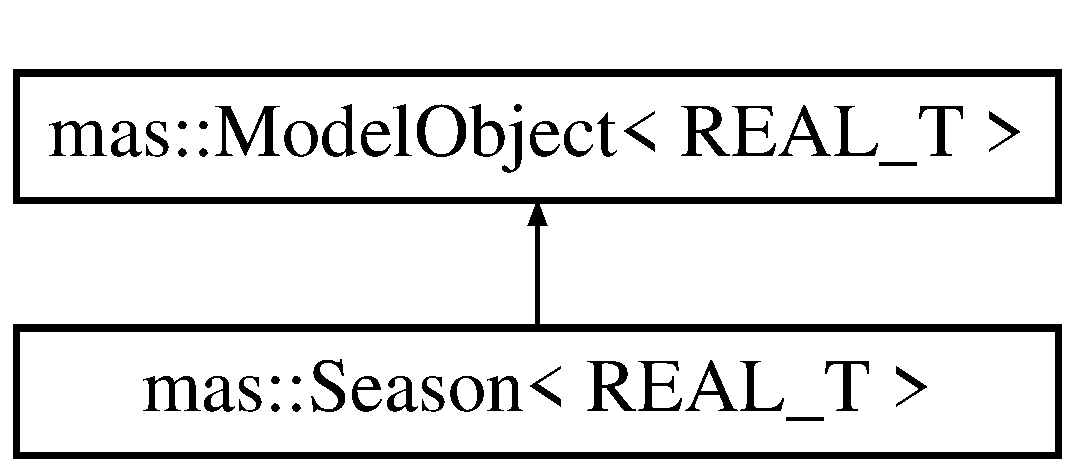
\includegraphics[height=2.000000cm]{structmas_1_1_season}
\end{center}
\end{figure}
\subsection*{Public Attributes}
\begin{DoxyCompactItemize}
\item 
std\-::string \hyperlink{structmas_1_1_season_a04a3d17eb36c71f3f5474468d2d73605}{name}
\item 
int \hyperlink{structmas_1_1_season_aad51659a30850ce9ee579e625ec0a212}{months}
\end{DoxyCompactItemize}
\subsection*{Additional Inherited Members}


\subsection{Detailed Description}
\subsubsection*{template$<$typename R\-E\-A\-L\-\_\-\-T$>$struct mas\-::\-Season$<$ R\-E\-A\-L\-\_\-\-T $>$}



Definition at line 41 of file Season.\-hpp.



\subsection{Member Data Documentation}
\hypertarget{structmas_1_1_season_aad51659a30850ce9ee579e625ec0a212}{\index{mas\-::\-Season@{mas\-::\-Season}!months@{months}}
\index{months@{months}!mas::Season@{mas\-::\-Season}}
\subsubsection[{months}]{\setlength{\rightskip}{0pt plus 5cm}template$<$typename R\-E\-A\-L\-\_\-\-T $>$ int {\bf mas\-::\-Season}$<$ R\-E\-A\-L\-\_\-\-T $>$\-::months}}\label{structmas_1_1_season_aad51659a30850ce9ee579e625ec0a212}


Definition at line 43 of file Season.\-hpp.

\hypertarget{structmas_1_1_season_a04a3d17eb36c71f3f5474468d2d73605}{\index{mas\-::\-Season@{mas\-::\-Season}!name@{name}}
\index{name@{name}!mas::Season@{mas\-::\-Season}}
\subsubsection[{name}]{\setlength{\rightskip}{0pt plus 5cm}template$<$typename R\-E\-A\-L\-\_\-\-T $>$ std\-::string {\bf mas\-::\-Season}$<$ R\-E\-A\-L\-\_\-\-T $>$\-::name}}\label{structmas_1_1_season_a04a3d17eb36c71f3f5474468d2d73605}


Definition at line 42 of file Season.\-hpp.



The documentation for this struct was generated from the following file\-:\begin{DoxyCompactItemize}
\item 
/home/oppy/\-Net\-Beans\-Projects/mas/\hyperlink{_season_8hpp}{Season.\-hpp}\end{DoxyCompactItemize}

\hypertarget{structmas_1_1_selectivity_base}{\section{mas\-:\-:Selectivity\-Base$<$ R\-E\-A\-L\-\_\-\-T $>$ Struct Template Reference}
\label{structmas_1_1_selectivity_base}\index{mas\-::\-Selectivity\-Base$<$ R\-E\-A\-L\-\_\-\-T $>$@{mas\-::\-Selectivity\-Base$<$ R\-E\-A\-L\-\_\-\-T $>$}}
}


{\ttfamily \#include $<$Selectivity.\-hpp$>$}

Inheritance diagram for mas\-:\-:Selectivity\-Base$<$ R\-E\-A\-L\-\_\-\-T $>$\-:\begin{figure}[H]
\begin{center}
\leavevmode
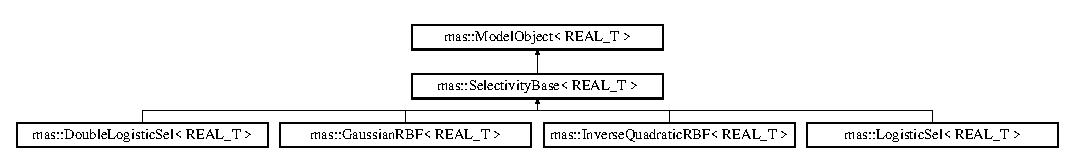
\includegraphics[height=1.750000cm]{structmas_1_1_selectivity_base}
\end{center}
\end{figure}
\subsection*{Public Types}
\begin{DoxyCompactItemize}
\item 
typedef \hyperlink{structmas_1_1_variable_trait}{Variable\-Trait}$<$ R\-E\-A\-L\-\_\-\-T $>$\\*
\-::\hyperlink{structmas_1_1_model_object_a4e62fdbb5826f8fac311262b888ab10a}{variable} \hyperlink{structmas_1_1_selectivity_base_a72a30a97f46039dc8b2161e4de308fee}{variable}
\end{DoxyCompactItemize}
\subsection*{Public Member Functions}
\begin{DoxyCompactItemize}
\item 
virtual const \hyperlink{structmas_1_1_model_object_a4e62fdbb5826f8fac311262b888ab10a}{variable} \hyperlink{structmas_1_1_selectivity_base_a1c26fb2107d380ac4540271280031bf4}{Evaluate} (const \hyperlink{structmas_1_1_model_object_a4e62fdbb5826f8fac311262b888ab10a}{variable} \&age)=0
\item 
virtual const \hyperlink{structmas_1_1_model_object_a4e62fdbb5826f8fac311262b888ab10a}{variable} \hyperlink{structmas_1_1_selectivity_base_a52058fc9fe373bcc6deebd43bfc3f402}{Evaluate} (const std\-::vector$<$ \hyperlink{structmas_1_1_model_object_a4e62fdbb5826f8fac311262b888ab10a}{variable} $>$ \&ages, size\-\_\-t index)=0
\item 
virtual const std\-::string \hyperlink{structmas_1_1_selectivity_base_ad14deefa4cddcc1c93ef17cc0a3e566a}{Name} ()
\end{DoxyCompactItemize}
\subsection*{Additional Inherited Members}


\subsection{Detailed Description}
\subsubsection*{template$<$typename R\-E\-A\-L\-\_\-\-T$>$struct mas\-::\-Selectivity\-Base$<$ R\-E\-A\-L\-\_\-\-T $>$}



Definition at line 41 of file Selectivity.\-hpp.



\subsection{Member Typedef Documentation}
\hypertarget{structmas_1_1_selectivity_base_a72a30a97f46039dc8b2161e4de308fee}{\index{mas\-::\-Selectivity\-Base@{mas\-::\-Selectivity\-Base}!variable@{variable}}
\index{variable@{variable}!mas::SelectivityBase@{mas\-::\-Selectivity\-Base}}
\subsubsection[{variable}]{\setlength{\rightskip}{0pt plus 5cm}template$<$typename R\-E\-A\-L\-\_\-\-T $>$ typedef {\bf Variable\-Trait}$<$R\-E\-A\-L\-\_\-\-T$>$\-::{\bf variable} {\bf mas\-::\-Selectivity\-Base}$<$ R\-E\-A\-L\-\_\-\-T $>$\-::{\bf variable}}}\label{structmas_1_1_selectivity_base_a72a30a97f46039dc8b2161e4de308fee}


Definition at line 42 of file Selectivity.\-hpp.



\subsection{Member Function Documentation}
\hypertarget{structmas_1_1_selectivity_base_a1c26fb2107d380ac4540271280031bf4}{\index{mas\-::\-Selectivity\-Base@{mas\-::\-Selectivity\-Base}!Evaluate@{Evaluate}}
\index{Evaluate@{Evaluate}!mas::SelectivityBase@{mas\-::\-Selectivity\-Base}}
\subsubsection[{Evaluate}]{\setlength{\rightskip}{0pt plus 5cm}template$<$typename R\-E\-A\-L\-\_\-\-T $>$ virtual const {\bf variable} {\bf mas\-::\-Selectivity\-Base}$<$ R\-E\-A\-L\-\_\-\-T $>$\-::Evaluate (
\begin{DoxyParamCaption}
\item[{const {\bf variable} \&}]{age}
\end{DoxyParamCaption}
)\hspace{0.3cm}{\ttfamily [pure virtual]}}}\label{structmas_1_1_selectivity_base_a1c26fb2107d380ac4540271280031bf4}


Implemented in \hyperlink{structmas_1_1_inverse_quadratic_r_b_f_a4753edb34b33f783ae2c645cc16a607c}{mas\-::\-Inverse\-Quadratic\-R\-B\-F$<$ R\-E\-A\-L\-\_\-\-T $>$}, \hyperlink{structmas_1_1_gaussian_r_b_f_a29fededb3644678ef80d7c65f601dfae}{mas\-::\-Gaussian\-R\-B\-F$<$ R\-E\-A\-L\-\_\-\-T $>$}, \hyperlink{structmas_1_1_double_logistic_sel_a90935c4bb22641c8e3f6e9e742c785ac}{mas\-::\-Double\-Logistic\-Sel$<$ R\-E\-A\-L\-\_\-\-T $>$}, and \hyperlink{structmas_1_1_logistic_sel_a2e7590748bd817f5a019c633213488cc}{mas\-::\-Logistic\-Sel$<$ R\-E\-A\-L\-\_\-\-T $>$}.

\hypertarget{structmas_1_1_selectivity_base_a52058fc9fe373bcc6deebd43bfc3f402}{\index{mas\-::\-Selectivity\-Base@{mas\-::\-Selectivity\-Base}!Evaluate@{Evaluate}}
\index{Evaluate@{Evaluate}!mas::SelectivityBase@{mas\-::\-Selectivity\-Base}}
\subsubsection[{Evaluate}]{\setlength{\rightskip}{0pt plus 5cm}template$<$typename R\-E\-A\-L\-\_\-\-T $>$ virtual const {\bf variable} {\bf mas\-::\-Selectivity\-Base}$<$ R\-E\-A\-L\-\_\-\-T $>$\-::Evaluate (
\begin{DoxyParamCaption}
\item[{const std\-::vector$<$ {\bf variable} $>$ \&}]{ages, }
\item[{size\-\_\-t}]{index}
\end{DoxyParamCaption}
)\hspace{0.3cm}{\ttfamily [pure virtual]}}}\label{structmas_1_1_selectivity_base_a52058fc9fe373bcc6deebd43bfc3f402}


Implemented in \hyperlink{structmas_1_1_inverse_quadratic_r_b_f_a326a1c19949fa3b309fbfc38a4c85dc7}{mas\-::\-Inverse\-Quadratic\-R\-B\-F$<$ R\-E\-A\-L\-\_\-\-T $>$}, \hyperlink{structmas_1_1_gaussian_r_b_f_a7710758db50657d20d5baf403713df87}{mas\-::\-Gaussian\-R\-B\-F$<$ R\-E\-A\-L\-\_\-\-T $>$}, \hyperlink{structmas_1_1_double_logistic_sel_ae6c78421dea075fd43bdd30ab0d8fad5}{mas\-::\-Double\-Logistic\-Sel$<$ R\-E\-A\-L\-\_\-\-T $>$}, and \hyperlink{structmas_1_1_logistic_sel_ae646dfffa37e9202381fb0c1879016ee}{mas\-::\-Logistic\-Sel$<$ R\-E\-A\-L\-\_\-\-T $>$}.

\hypertarget{structmas_1_1_selectivity_base_ad14deefa4cddcc1c93ef17cc0a3e566a}{\index{mas\-::\-Selectivity\-Base@{mas\-::\-Selectivity\-Base}!Name@{Name}}
\index{Name@{Name}!mas::SelectivityBase@{mas\-::\-Selectivity\-Base}}
\subsubsection[{Name}]{\setlength{\rightskip}{0pt plus 5cm}template$<$typename R\-E\-A\-L\-\_\-\-T $>$ virtual const std\-::string {\bf mas\-::\-Selectivity\-Base}$<$ R\-E\-A\-L\-\_\-\-T $>$\-::Name (
\begin{DoxyParamCaption}
{}
\end{DoxyParamCaption}
)\hspace{0.3cm}{\ttfamily [inline]}, {\ttfamily [virtual]}}}\label{structmas_1_1_selectivity_base_ad14deefa4cddcc1c93ef17cc0a3e566a}


Reimplemented in \hyperlink{structmas_1_1_inverse_quadratic_r_b_f_a2733866b50a4a7ae667f50334fdccc27}{mas\-::\-Inverse\-Quadratic\-R\-B\-F$<$ R\-E\-A\-L\-\_\-\-T $>$}, \hyperlink{structmas_1_1_gaussian_r_b_f_a41b0813587b13d6b62dc5eedac91cc93}{mas\-::\-Gaussian\-R\-B\-F$<$ R\-E\-A\-L\-\_\-\-T $>$}, \hyperlink{structmas_1_1_double_logistic_sel_a1f71e8df42eb1d1b7b54df4e0427d05b}{mas\-::\-Double\-Logistic\-Sel$<$ R\-E\-A\-L\-\_\-\-T $>$}, and \hyperlink{structmas_1_1_logistic_sel_a58f669fc791e7e86ef70820dbbed35ba}{mas\-::\-Logistic\-Sel$<$ R\-E\-A\-L\-\_\-\-T $>$}.



Definition at line 50 of file Selectivity.\-hpp.



The documentation for this struct was generated from the following file\-:\begin{DoxyCompactItemize}
\item 
/home/oppy/\-Net\-Beans\-Projects/mas/\hyperlink{_selectivity_8hpp}{Selectivity.\-hpp}\end{DoxyCompactItemize}

\hypertarget{structmas_1_1_shepherd}{\section{mas\-:\-:Shepherd$<$ R\-E\-A\-L\-\_\-\-T $>$ Struct Template Reference}
\label{structmas_1_1_shepherd}\index{mas\-::\-Shepherd$<$ R\-E\-A\-L\-\_\-\-T $>$@{mas\-::\-Shepherd$<$ R\-E\-A\-L\-\_\-\-T $>$}}
}


{\ttfamily \#include $<$Recruitment.\-hpp$>$}

Inheritance diagram for mas\-:\-:Shepherd$<$ R\-E\-A\-L\-\_\-\-T $>$\-:\begin{figure}[H]
\begin{center}
\leavevmode
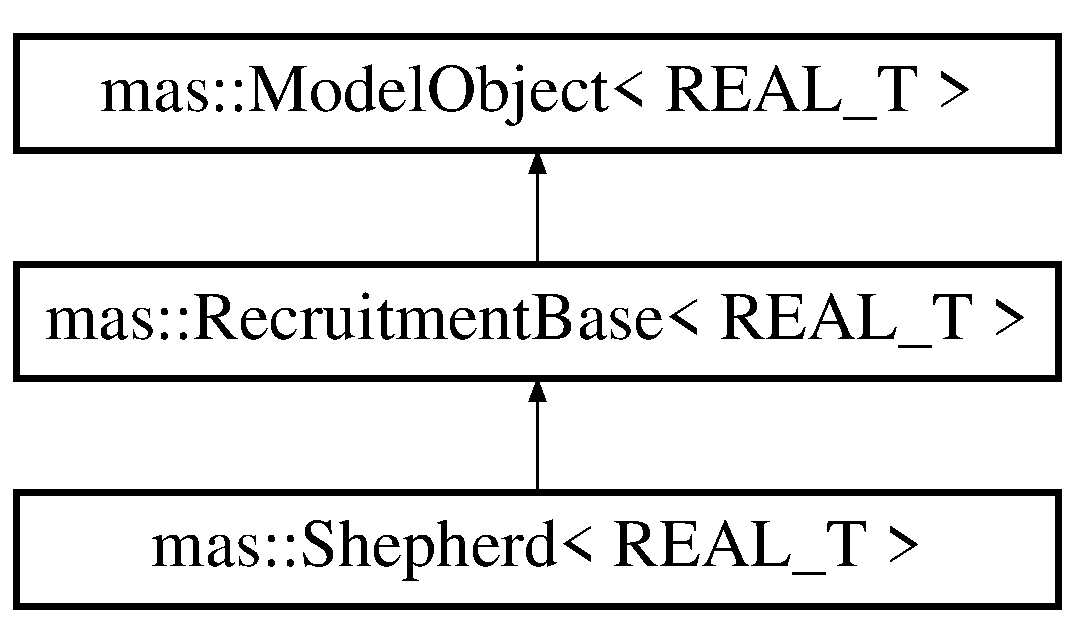
\includegraphics[height=3.000000cm]{structmas_1_1_shepherd}
\end{center}
\end{figure}
\subsection*{Public Types}
\begin{DoxyCompactItemize}
\item 
typedef \hyperlink{structmas_1_1_variable_trait}{Variable\-Trait}$<$ R\-E\-A\-L\-\_\-\-T $>$\\*
\-::\hyperlink{structmas_1_1_shepherd_a5d9d0045570bba5f3450dcedea6a406e}{variable} \hyperlink{structmas_1_1_shepherd_a5d9d0045570bba5f3450dcedea6a406e}{variable}
\end{DoxyCompactItemize}
\subsection*{Public Member Functions}
\begin{DoxyCompactItemize}
\item 
const \hyperlink{structmas_1_1_shepherd_a5d9d0045570bba5f3450dcedea6a406e}{variable} \hyperlink{structmas_1_1_shepherd_a0e7a914d27be18b2c9efa052958d1f0b}{Evaluate} (const int \&pop\-\_\-id, const int \&area\-\_\-id, const \hyperlink{structmas_1_1_shepherd_a5d9d0045570bba5f3450dcedea6a406e}{variable} \&s)
\item 
virtual const std\-::string \hyperlink{structmas_1_1_shepherd_aafe14075a992d9157bc8594aac0a2eeb}{To\-J\-S\-O\-N\-String} ()
\item 
virtual const std\-::string \hyperlink{structmas_1_1_shepherd_aed20558dd1e310073ebba7968fe5f36f}{Name} ()
\end{DoxyCompactItemize}
\subsection*{Public Attributes}
\begin{DoxyCompactItemize}
\item 
\hyperlink{structmas_1_1_shepherd_a5d9d0045570bba5f3450dcedea6a406e}{variable} \hyperlink{structmas_1_1_shepherd_a24f215424f8fe3e38ce0b26fd09628bf}{alpha}
\item 
\hyperlink{structmas_1_1_shepherd_a5d9d0045570bba5f3450dcedea6a406e}{variable} \hyperlink{structmas_1_1_shepherd_a40725fc01050b72af7e0573da6ca2d55}{beta}
\item 
\hyperlink{structmas_1_1_shepherd_a5d9d0045570bba5f3450dcedea6a406e}{variable} \hyperlink{structmas_1_1_shepherd_ab9a9d636240bb7b6b3cea58a85fc5435}{c}
\end{DoxyCompactItemize}


\subsection{Detailed Description}
\subsubsection*{template$<$typename R\-E\-A\-L\-\_\-\-T$>$struct mas\-::\-Shepherd$<$ R\-E\-A\-L\-\_\-\-T $>$}



Definition at line 294 of file Recruitment.\-hpp.



\subsection{Member Typedef Documentation}
\hypertarget{structmas_1_1_shepherd_a5d9d0045570bba5f3450dcedea6a406e}{\index{mas\-::\-Shepherd@{mas\-::\-Shepherd}!variable@{variable}}
\index{variable@{variable}!mas::Shepherd@{mas\-::\-Shepherd}}
\subsubsection[{variable}]{\setlength{\rightskip}{0pt plus 5cm}template$<$typename R\-E\-A\-L\-\_\-\-T $>$ typedef {\bf Variable\-Trait}$<$R\-E\-A\-L\-\_\-\-T$>$\-::{\bf variable} {\bf mas\-::\-Shepherd}$<$ R\-E\-A\-L\-\_\-\-T $>$\-::{\bf variable}}}\label{structmas_1_1_shepherd_a5d9d0045570bba5f3450dcedea6a406e}


Definition at line 295 of file Recruitment.\-hpp.



\subsection{Member Function Documentation}
\hypertarget{structmas_1_1_shepherd_a0e7a914d27be18b2c9efa052958d1f0b}{\index{mas\-::\-Shepherd@{mas\-::\-Shepherd}!Evaluate@{Evaluate}}
\index{Evaluate@{Evaluate}!mas::Shepherd@{mas\-::\-Shepherd}}
\subsubsection[{Evaluate}]{\setlength{\rightskip}{0pt plus 5cm}template$<$typename R\-E\-A\-L\-\_\-\-T $>$ const {\bf variable} {\bf mas\-::\-Shepherd}$<$ R\-E\-A\-L\-\_\-\-T $>$\-::Evaluate (
\begin{DoxyParamCaption}
\item[{const int \&}]{pop\-\_\-id, }
\item[{const int \&}]{area\-\_\-id, }
\item[{const {\bf variable} \&}]{s}
\end{DoxyParamCaption}
)\hspace{0.3cm}{\ttfamily [inline]}, {\ttfamily [virtual]}}}\label{structmas_1_1_shepherd_a0e7a914d27be18b2c9efa052958d1f0b}


Implements \hyperlink{structmas_1_1_recruitment_base_a74a7f9dd7090f156c6a5068ce29f53ff}{mas\-::\-Recruitment\-Base$<$ R\-E\-A\-L\-\_\-\-T $>$}.



Definition at line 300 of file Recruitment.\-hpp.

\hypertarget{structmas_1_1_shepherd_aed20558dd1e310073ebba7968fe5f36f}{\index{mas\-::\-Shepherd@{mas\-::\-Shepherd}!Name@{Name}}
\index{Name@{Name}!mas::Shepherd@{mas\-::\-Shepherd}}
\subsubsection[{Name}]{\setlength{\rightskip}{0pt plus 5cm}template$<$typename R\-E\-A\-L\-\_\-\-T $>$ virtual const std\-::string {\bf mas\-::\-Shepherd}$<$ R\-E\-A\-L\-\_\-\-T $>$\-::Name (
\begin{DoxyParamCaption}
{}
\end{DoxyParamCaption}
)\hspace{0.3cm}{\ttfamily [inline]}, {\ttfamily [virtual]}}}\label{structmas_1_1_shepherd_aed20558dd1e310073ebba7968fe5f36f}


Reimplemented from \hyperlink{structmas_1_1_recruitment_base_abfdd47e97127a35f81d441ac3e1afaec}{mas\-::\-Recruitment\-Base$<$ R\-E\-A\-L\-\_\-\-T $>$}.



Definition at line 324 of file Recruitment.\-hpp.

\hypertarget{structmas_1_1_shepherd_aafe14075a992d9157bc8594aac0a2eeb}{\index{mas\-::\-Shepherd@{mas\-::\-Shepherd}!To\-J\-S\-O\-N\-String@{To\-J\-S\-O\-N\-String}}
\index{To\-J\-S\-O\-N\-String@{To\-J\-S\-O\-N\-String}!mas::Shepherd@{mas\-::\-Shepherd}}
\subsubsection[{To\-J\-S\-O\-N\-String}]{\setlength{\rightskip}{0pt plus 5cm}template$<$typename R\-E\-A\-L\-\_\-\-T $>$ virtual const std\-::string {\bf mas\-::\-Shepherd}$<$ R\-E\-A\-L\-\_\-\-T $>$\-::To\-J\-S\-O\-N\-String (
\begin{DoxyParamCaption}
{}
\end{DoxyParamCaption}
)\hspace{0.3cm}{\ttfamily [inline]}, {\ttfamily [virtual]}}}\label{structmas_1_1_shepherd_aafe14075a992d9157bc8594aac0a2eeb}


Reimplemented from \hyperlink{structmas_1_1_model_object_af40b3c89b11919fc5aea21dcf1cd027b}{mas\-::\-Model\-Object$<$ R\-E\-A\-L\-\_\-\-T $>$}.



Definition at line 304 of file Recruitment.\-hpp.



\subsection{Member Data Documentation}
\hypertarget{structmas_1_1_shepherd_a24f215424f8fe3e38ce0b26fd09628bf}{\index{mas\-::\-Shepherd@{mas\-::\-Shepherd}!alpha@{alpha}}
\index{alpha@{alpha}!mas::Shepherd@{mas\-::\-Shepherd}}
\subsubsection[{alpha}]{\setlength{\rightskip}{0pt plus 5cm}template$<$typename R\-E\-A\-L\-\_\-\-T $>$ {\bf variable} {\bf mas\-::\-Shepherd}$<$ R\-E\-A\-L\-\_\-\-T $>$\-::alpha}}\label{structmas_1_1_shepherd_a24f215424f8fe3e38ce0b26fd09628bf}


Definition at line 296 of file Recruitment.\-hpp.

\hypertarget{structmas_1_1_shepherd_a40725fc01050b72af7e0573da6ca2d55}{\index{mas\-::\-Shepherd@{mas\-::\-Shepherd}!beta@{beta}}
\index{beta@{beta}!mas::Shepherd@{mas\-::\-Shepherd}}
\subsubsection[{beta}]{\setlength{\rightskip}{0pt plus 5cm}template$<$typename R\-E\-A\-L\-\_\-\-T $>$ {\bf variable} {\bf mas\-::\-Shepherd}$<$ R\-E\-A\-L\-\_\-\-T $>$\-::beta}}\label{structmas_1_1_shepherd_a40725fc01050b72af7e0573da6ca2d55}


Definition at line 297 of file Recruitment.\-hpp.

\hypertarget{structmas_1_1_shepherd_ab9a9d636240bb7b6b3cea58a85fc5435}{\index{mas\-::\-Shepherd@{mas\-::\-Shepherd}!c@{c}}
\index{c@{c}!mas::Shepherd@{mas\-::\-Shepherd}}
\subsubsection[{c}]{\setlength{\rightskip}{0pt plus 5cm}template$<$typename R\-E\-A\-L\-\_\-\-T $>$ {\bf variable} {\bf mas\-::\-Shepherd}$<$ R\-E\-A\-L\-\_\-\-T $>$\-::c}}\label{structmas_1_1_shepherd_ab9a9d636240bb7b6b3cea58a85fc5435}


Definition at line 298 of file Recruitment.\-hpp.



The documentation for this struct was generated from the following file\-:\begin{DoxyCompactItemize}
\item 
/home/oppy/\-Net\-Beans\-Projects/mas/\hyperlink{_recruitment_8hpp}{Recruitment.\-hpp}\end{DoxyCompactItemize}

\hypertarget{structmas_1_1_survey}{\section{mas\-:\-:Survey$<$ R\-E\-A\-L\-\_\-\-T $>$ Struct Template Reference}
\label{structmas_1_1_survey}\index{mas\-::\-Survey$<$ R\-E\-A\-L\-\_\-\-T $>$@{mas\-::\-Survey$<$ R\-E\-A\-L\-\_\-\-T $>$}}
}


{\ttfamily \#include $<$Survey.\-hpp$>$}

Inheritance diagram for mas\-:\-:Survey$<$ R\-E\-A\-L\-\_\-\-T $>$\-:\begin{figure}[H]
\begin{center}
\leavevmode
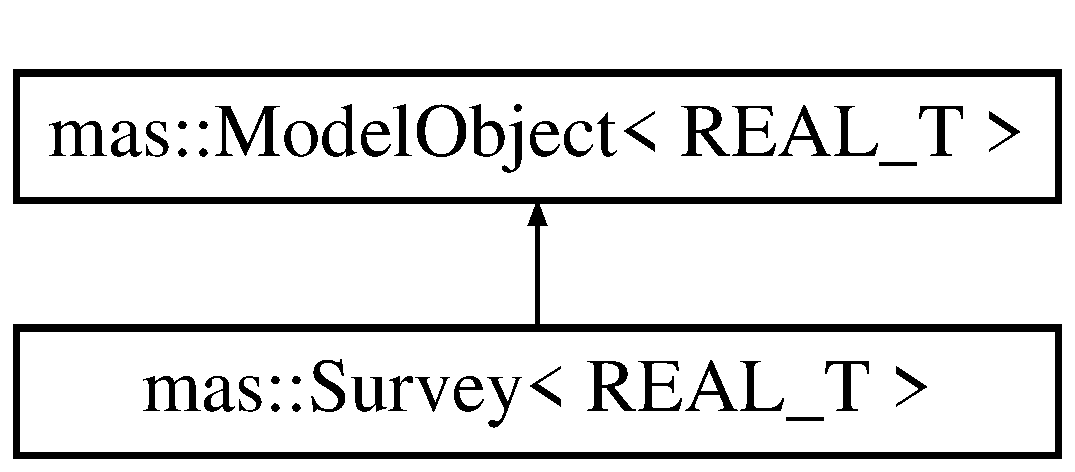
\includegraphics[height=2.000000cm]{structmas_1_1_survey}
\end{center}
\end{figure}
\subsection*{Public Types}
\begin{DoxyCompactItemize}
\item 
typedef \hyperlink{structmas_1_1_variable_trait}{Variable\-Trait}$<$ R\-E\-A\-L\-\_\-\-T $>$\\*
\-::\hyperlink{structmas_1_1_survey_ae91896013e1a3403f7e3d79b1f845966}{variable} \hyperlink{structmas_1_1_survey_ae91896013e1a3403f7e3d79b1f845966}{variable}
\item 
typedef std\-::unordered\-\_\-map\\*
$<$ int, std\-::unordered\-\_\-map$<$ int, \\*
int $>$ $>$\-::iterator \hyperlink{structmas_1_1_survey_a93b422e50a88d61d2bf59e5cf8895295}{season\-\_\-area\-\_\-selectivity\-\_\-ids\-\_\-iterator}
\item 
typedef std\-::unordered\-\_\-map\\*
$<$ int, std\-::unordered\-\_\-map$<$ int, \\*
int $>$ $>$\-::const\-\_\-iterator \hyperlink{structmas_1_1_survey_af8b1532c87b7b6cce73d17472d03eb5a}{season\-\_\-area\-\_\-selectivity\-\_\-ids\-\_\-const\-\_\-iterator}
\item 
typedef std\-::unordered\-\_\-map\\*
$<$ int, std\-::shared\-\_\-ptr\\*
$<$ \hyperlink{structmas_1_1_selectivity_base}{mas\-::\-Selectivity\-Base}$<$ R\-E\-A\-L\-\_\-\-T $>$\\*
 $>$ $>$\-::iterator \hyperlink{structmas_1_1_survey_abfde314e73f8c92d58d75373fc805ee3}{area\-\_\-sectivity\-\_\-iterator}
\item 
typedef std\-::unordered\-\_\-map\\*
$<$ int, std\-::unordered\-\_\-map$<$ int, \\*
int $>$ $>$\-::iterator \hyperlink{structmas_1_1_survey_aabb40313de7f308ef66d028b839984ca}{season\-\_\-area\-\_\-id\-\_\-iterator}
\item 
typedef std\-::unordered\-\_\-map\\*
$<$ int, int $>$\-::iterator \hyperlink{structmas_1_1_survey_a08455055f86587e069b3ea5266ef0822}{area\-\_\-id\-\_\-iteraor}
\item 
typedef std\-::unordered\-\_\-map\\*
$<$ int, int $>$\-::iterator \hyperlink{structmas_1_1_survey_a609a3e09a088bcc4f5bed6fdb565566e}{season\-\_\-id\-\_\-iteraor}
\item 
typedef std\-::unordered\-\_\-map\\*
$<$ int, std\-::unordered\-\_\-map$<$ int, \\*
std\-::shared\-\_\-ptr\\*
$<$ \hyperlink{structmas_1_1_selectivity_base}{mas\-::\-Selectivity\-Base}$<$ R\-E\-A\-L\-\_\-\-T $>$\\*
 $>$ $>$ $>$\-::iterator \hyperlink{structmas_1_1_survey_a75fb76cac18f90a25965ce77bdb6b429}{season\-\_\-area\-\_\-selectivity\-\_\-iterator}
\end{DoxyCompactItemize}
\subsection*{Public Member Functions}
\begin{DoxyCompactItemize}
\item 
void \hyperlink{structmas_1_1_survey_a853afce2d38c57ee46992f3a72b8d30e}{Initialize} (size\-\_\-t \hyperlink{structmas_1_1_survey_a62db9142400baea1e578c34ffa423d97}{years}, size\-\_\-t \hyperlink{structmas_1_1_survey_a823552ecb1c304d152b0befca7465394}{seasons}, size\-\_\-t \hyperlink{structmas_1_1_survey_a00478a5d1bf1272d220efde6560efe06}{ages})
\item 
void \hyperlink{structmas_1_1_survey_a9ffa08005fb5d846348be88e2103a298}{Initialize\-N\-L\-L\-Components} ()
\item 
void \hyperlink{structmas_1_1_survey_add6927885e43a0fcd5c538d6fe82ca42}{Prepare} ()
\item 
void \hyperlink{structmas_1_1_survey_ae32a9c02bbcc53e3d2146ddcb32eaed3}{Compute\-Proportions} ()
\item 
void \hyperlink{structmas_1_1_survey_a4608e42779725ea5d7f50b6b36758b25}{Compute\-N\-L\-L\-Components} ()
\item 
void \hyperlink{structmas_1_1_survey_ab152b25450461b5e23f3b9d862c77bfb}{Compute\-Goodness\-Of\-Fit} ()
\item 
void \hyperlink{structmas_1_1_survey_a895cdad735876fbf96584b20cdf81833}{Evaluate\-Biomass\-Component} (int year, int season)
\item 
void \hyperlink{structmas_1_1_survey_a8da55cc79c09a0a647369f6359157c92}{Evaluate\-Age\-Comp\-Component} (int year, int season)
\end{DoxyCompactItemize}
\subsection*{Public Attributes}
\begin{DoxyCompactItemize}
\item 
int \hyperlink{structmas_1_1_survey_a0e0e24656b837749042a9ed368a61aa6}{id}
\item 
int \hyperlink{structmas_1_1_survey_a62db9142400baea1e578c34ffa423d97}{years}
\item 
int \hyperlink{structmas_1_1_survey_a823552ecb1c304d152b0befca7465394}{seasons}
\item 
int \hyperlink{structmas_1_1_survey_a00478a5d1bf1272d220efde6560efe06}{ages}
\item 
std\-::vector$<$ \hyperlink{structmas_1_1_survey_ae91896013e1a3403f7e3d79b1f845966}{variable} $>$ \hyperlink{structmas_1_1_survey_ae17e461c7ac75c48a2dd5cd80d17d485}{survey\-\_\-biomass\-\_\-total}
\item 
std\-::vector$<$ \hyperlink{structmas_1_1_survey_ae91896013e1a3403f7e3d79b1f845966}{variable} $>$ \hyperlink{structmas_1_1_survey_ab6e2c544df4e59bc1b4169132dc598b6}{survey\-\_\-biomass\-\_\-total\-\_\-males}
\item 
std\-::vector$<$ \hyperlink{structmas_1_1_survey_ae91896013e1a3403f7e3d79b1f845966}{variable} $>$ \hyperlink{structmas_1_1_survey_a2a3551f2c4083ca4ec39f40d2afc3dc5}{survey\-\_\-biomass\-\_\-total\-\_\-females}
\item 
std\-::vector$<$ \hyperlink{structmas_1_1_survey_ae91896013e1a3403f7e3d79b1f845966}{variable} $>$ \hyperlink{structmas_1_1_survey_a84b8d86778e01e5deae1b89b21dd9101}{survey\-\_\-numbers\-\_\-at\-\_\-age}
\item 
std\-::vector$<$ \hyperlink{structmas_1_1_survey_ae91896013e1a3403f7e3d79b1f845966}{variable} $>$ \hyperlink{structmas_1_1_survey_a80b8b0dec9dfd6cf78ab807eaa1aa446}{survey\-\_\-biomass\-\_\-at\-\_\-age}
\item 
std\-::vector$<$ \hyperlink{structmas_1_1_survey_ae91896013e1a3403f7e3d79b1f845966}{variable} $>$ \hyperlink{structmas_1_1_survey_aea931b487380dc2188543c50c50e101c}{survey\-\_\-proportion\-\_\-at\-\_\-age}
\item 
std\-::vector$<$ \hyperlink{structmas_1_1_survey_ae91896013e1a3403f7e3d79b1f845966}{variable} $>$ \hyperlink{structmas_1_1_survey_a6f6ec205376fb1a8d629117bd8e4a1d6}{survey\-\_\-biomass\-\_\-proportion\-\_\-at\-\_\-age}
\item 
std\-::vector$<$ \hyperlink{structmas_1_1_survey_ae91896013e1a3403f7e3d79b1f845966}{variable} $>$ \hyperlink{structmas_1_1_survey_a2727239747456825885406d15a07c08d}{survey\-\_\-numbers\-\_\-at\-\_\-age\-\_\-males}
\item 
std\-::vector$<$ \hyperlink{structmas_1_1_survey_ae91896013e1a3403f7e3d79b1f845966}{variable} $>$ \hyperlink{structmas_1_1_survey_a65aa83d0a4c0e33a58f933b7712aea76}{survey\-\_\-biomass\-\_\-at\-\_\-age\-\_\-males}
\item 
std\-::vector$<$ \hyperlink{structmas_1_1_survey_ae91896013e1a3403f7e3d79b1f845966}{variable} $>$ \hyperlink{structmas_1_1_survey_ab22021d23ed4557342ebf3af305e95b6}{survey\-\_\-proportion\-\_\-at\-\_\-age\-\_\-males}
\item 
std\-::vector$<$ \hyperlink{structmas_1_1_survey_ae91896013e1a3403f7e3d79b1f845966}{variable} $>$ \hyperlink{structmas_1_1_survey_a81ba97fe092ee36ab133aa4416a883d4}{survey\-\_\-biomass\-\_\-proportion\-\_\-at\-\_\-age\-\_\-males}
\item 
std\-::vector$<$ \hyperlink{structmas_1_1_survey_ae91896013e1a3403f7e3d79b1f845966}{variable} $>$ \hyperlink{structmas_1_1_survey_ab098ff5aa484ec1564b4dbaf9c9df95c}{survey\-\_\-numbers\-\_\-at\-\_\-age\-\_\-females}
\item 
std\-::vector$<$ \hyperlink{structmas_1_1_survey_ae91896013e1a3403f7e3d79b1f845966}{variable} $>$ \hyperlink{structmas_1_1_survey_a150871da567d1b9e5bd7835537a1ae94}{survey\-\_\-biomass\-\_\-at\-\_\-age\-\_\-females}
\item 
std\-::vector$<$ \hyperlink{structmas_1_1_survey_ae91896013e1a3403f7e3d79b1f845966}{variable} $>$ \hyperlink{structmas_1_1_survey_a8e55c1393d70b3354b7670ed20065af4}{survey\-\_\-proportion\-\_\-at\-\_\-age\-\_\-females}
\item 
std\-::vector$<$ \hyperlink{structmas_1_1_survey_ae91896013e1a3403f7e3d79b1f845966}{variable} $>$ \hyperlink{structmas_1_1_survey_a686876186e69ee392fb4ce0a481863ee}{survey\-\_\-biomass\-\_\-proportion\-\_\-at\-\_\-age\-\_\-females}
\item 
std\-::vector$<$ \hyperlink{structmas_1_1_survey_ae91896013e1a3403f7e3d79b1f845966}{variable} $>$ \hyperlink{structmas_1_1_survey_aa01ce2732a42f7580f1803cef493370f}{S\-N\-\_\-diff2}
\item 
std\-::vector$<$ \hyperlink{structmas_1_1_survey_ae91896013e1a3403f7e3d79b1f845966}{variable} $>$ \hyperlink{structmas_1_1_survey_a3394b3a1fbc6ac6c788cde5411b6e9e3}{S\-N\-\_\-\-Biomass\-\_\-diff2}
\item 
std\-::vector$<$ \hyperlink{structmas_1_1_survey_ae91896013e1a3403f7e3d79b1f845966}{variable} $>$ \hyperlink{structmas_1_1_survey_ad8f4967194f0217375577ef06e99df73}{S\-N\-\_\-\-Proportion\-\_\-diff2}
\item 
std\-::vector$<$ \hyperlink{structmas_1_1_survey_ae91896013e1a3403f7e3d79b1f845966}{variable} $>$ \hyperlink{structmas_1_1_survey_a2b909685f664b5453d5dfb38b84452cf}{S\-N\-\_\-\-Biomass\-\_\-\-Proportion\-\_\-diff2}
\item 
std\-::string \hyperlink{structmas_1_1_survey_a8fd8098e67c99e6dbd98ebad552693ee}{name}
\item 
int \hyperlink{structmas_1_1_survey_a6c064392c7b16513028547c473c612d4}{population}
\item 
int \hyperlink{structmas_1_1_survey_ab8a937f0a4f30704ad3d096389df45ae}{selectivity\-\_\-model\-\_\-id}
\item 
std\-::vector$<$ int $>$ \hyperlink{structmas_1_1_survey_a8aeefcfbec9baeea0786200f888da11f}{area\-\_\-ids}
\item 
std\-::shared\-\_\-ptr$<$ \hyperlink{structmas_1_1_data_object}{Data\-Object}\\*
$<$ R\-E\-A\-L\-\_\-\-T $>$ $>$ \hyperlink{structmas_1_1_survey_aed7561a0147e5abfa07acab7baa9292f}{survey\-\_\-biomass\-\_\-data}
\item 
std\-::shared\-\_\-ptr$<$ \hyperlink{structmas_1_1_data_object}{Data\-Object}\\*
$<$ R\-E\-A\-L\-\_\-\-T $>$ $>$ \hyperlink{structmas_1_1_survey_a5f29ffd1fbe8b5038854a1fce1204d04}{survey\-\_\-proportion\-\_\-at\-\_\-age\-\_\-data\-\_\-\-N}
\item 
std\-::shared\-\_\-ptr$<$ \hyperlink{structmas_1_1_data_object}{Data\-Object}\\*
$<$ R\-E\-A\-L\-\_\-\-T $>$ $>$ \hyperlink{structmas_1_1_survey_abe5be20bcd63fb69b91008672bcb76ff}{survey\-\_\-proportion\-\_\-at\-\_\-age\-\_\-data}
\item 
std\-::shared\-\_\-ptr$<$ \hyperlink{structmas_1_1_data_object}{Data\-Object}\\*
$<$ R\-E\-A\-L\-\_\-\-T $>$ $>$ \hyperlink{structmas_1_1_survey_a0b400422f471584cfb574d98fe54a5cc}{survey\-\_\-proportion\-\_\-at\-\_\-length\-\_\-data\-\_\-\-N}
\item 
std\-::shared\-\_\-ptr$<$ \hyperlink{structmas_1_1_data_object}{Data\-Object}\\*
$<$ R\-E\-A\-L\-\_\-\-T $>$ $>$ \hyperlink{structmas_1_1_survey_a12418ba69c060c3778d723ad162dd1ba}{survey\-\_\-proportion\-\_\-at\-\_\-length\-\_\-data}
\item 
std\-::shared\-\_\-ptr$<$ \hyperlink{structmas_1_1_data_object}{Data\-Object}\\*
$<$ R\-E\-A\-L\-\_\-\-T $>$ $>$ \hyperlink{structmas_1_1_survey_a32474f16bef5d94a531f52dbd91b2305}{survey\-\_\-mean\-\_\-size\-\_\-at\-\_\-age\-\_\-data}
\item 
std\-::shared\-\_\-ptr$<$ \hyperlink{structmas_1_1_data_object}{Data\-Object}\\*
$<$ R\-E\-A\-L\-\_\-\-T $>$ $>$ \hyperlink{structmas_1_1_survey_ad01d8e1c386d36f34c352238f78f4ead}{survey\-\_\-mean\-\_\-weight\-\_\-at\-\_\-age\-\_\-data}
\item 
std\-::vector$<$ std\-::shared\-\_\-ptr\\*
$<$ \hyperlink{structmas_1_1_data_object}{Data\-Object}$<$ R\-E\-A\-L\-\_\-\-T $>$ $>$ $>$ \hyperlink{structmas_1_1_survey_a2dd1a625771db3a41ed2a050a984beeb}{data\-\_\-objects}
\item 
std\-::shared\-\_\-ptr\\*
$<$ \hyperlink{structmas_1_1_selectivity_base}{mas\-::\-Selectivity\-Base}$<$ R\-E\-A\-L\-\_\-\-T $>$ $>$ \hyperlink{structmas_1_1_survey_a798139029887e8727481a8f76b261ee0}{selectivity}
\item 
std\-::unordered\-\_\-map$<$ int, \\*
std\-::unordered\-\_\-map$<$ int, int $>$ $>$ \hyperlink{structmas_1_1_survey_a0b41369965fde2f49c1511a38a60447a}{area\-\_\-season\-\_\-selectivity\-\_\-ids}
\item 
std\-::unordered\-\_\-map$<$ int, \\*
std\-::unordered\-\_\-map$<$ int, \\*
std\-::shared\-\_\-ptr\\*
$<$ \hyperlink{structmas_1_1_selectivity_base}{mas\-::\-Selectivity\-Base}$<$ R\-E\-A\-L\-\_\-\-T $>$ $>$ $>$ $>$ \hyperlink{structmas_1_1_survey_af401401f9a2b3e9ca1e37a94f04db0c4}{area\-\_\-season\-\_\-selectivity}
\item 
std\-::unordered\-\_\-map$<$ int, \\*
std\-::unordered\-\_\-map$<$ int, int $>$ $>$ \hyperlink{structmas_1_1_survey_ad34128c8609aa9f7a2d37e8f484bb70b}{season\-\_\-area\-\_\-selectivity\-\_\-ids}
\item 
std\-::unordered\-\_\-map$<$ int, \\*
std\-::unordered\-\_\-map$<$ int, \\*
std\-::shared\-\_\-ptr\\*
$<$ \hyperlink{structmas_1_1_selectivity_base}{mas\-::\-Selectivity\-Base}$<$ R\-E\-A\-L\-\_\-\-T $>$ $>$ $>$ $>$ \hyperlink{structmas_1_1_survey_a7c006caaf702a6288b3c6ff2407af3b1}{season\-\_\-area\-\_\-selectivity}
\item 
std\-::unordered\-\_\-map$<$ int, \\*
std\-::unordered\-\_\-map$<$ int, \\*
std\-::shared\-\_\-ptr$<$ \hyperlink{structmas_1_1_area}{mas\-::\-Area}\\*
$<$ R\-E\-A\-L\-\_\-\-T $>$ $>$ $>$ $>$ \hyperlink{structmas_1_1_survey_a6ecd9fe4f0b4d75b3801e6f74ca75029}{seasonal\-\_\-areas\-\_\-of\-\_\-operation}
\item 
R\-E\-A\-L\-\_\-\-T \hyperlink{structmas_1_1_survey_a60c73865d0f6db4aa33cfd314b77882e}{survey\-\_\-fraction\-\_\-of\-\_\-year} = 0.\-75
\item 
R\-E\-A\-L\-\_\-\-T \hyperlink{structmas_1_1_survey_aad907f4e8413369d6f747f575dca2c91}{srv\-\_\-\-C\-V} = .\-2
\item 
\hyperlink{structmas_1_1_survey_ae91896013e1a3403f7e3d79b1f845966}{variable} \hyperlink{structmas_1_1_survey_a6c5894f588689dc14a54b218da5f6663}{q}
\item 
\hyperlink{structmas_1_1_survey_ae91896013e1a3403f7e3d79b1f845966}{variable} \hyperlink{structmas_1_1_survey_ad2cbd5ec4cb7f54ee7312fd1dece26c4}{survey\-\_\-biomass\-\_\-component}
\item 
\hyperlink{structmas_1_1_survey_ae91896013e1a3403f7e3d79b1f845966}{variable} \hyperlink{structmas_1_1_survey_afa960c2c4912f01084664b99fd9bf736}{survey\-\_\-age\-\_\-comp\-\_\-component}
\item 
int \hyperlink{structmas_1_1_survey_ab091939f1b686d7dcbaf00ac9a2b507e}{survey\-\_\-age\-\_\-comp\-\_\-likelihood\-\_\-component\-\_\-id} = -\/999
\item 
std\-::shared\-\_\-ptr\\*
$<$ \hyperlink{structmas_1_1_n_l_l_functor}{mas\-::\-N\-L\-L\-Functor}$<$ R\-E\-A\-L\-\_\-\-T $>$ $>$ \hyperlink{structmas_1_1_survey_a913143ad9c3da583b3cad6f1a1ab109c}{survey\-\_\-age\-\_\-comp\-\_\-likelihood\-\_\-component}
\item 
int \hyperlink{structmas_1_1_survey_a4bb22fe02896841ef41d76172e0a8f91}{survey\-\_\-biomass\-\_\-likelihood\-\_\-component\-\_\-id} = -\/999
\item 
std\-::shared\-\_\-ptr\\*
$<$ \hyperlink{structmas_1_1_n_l_l_functor}{mas\-::\-N\-L\-L\-Functor}$<$ R\-E\-A\-L\-\_\-\-T $>$ $>$ \hyperlink{structmas_1_1_survey_abee83156dc5c12a911adc3e107931d3d}{survey\-\_\-biomass\-\_\-likelihood\-\_\-component}
\item 
R\-E\-A\-L\-\_\-\-T \hyperlink{structmas_1_1_survey_a6cfcc6ed9b540be83a61cb44e7285d79}{survey\-\_\-biomass\-\_\-chi\-\_\-squared}
\item 
R\-E\-A\-L\-\_\-\-T \hyperlink{structmas_1_1_survey_acd94359a531d576cfbbe7d5a1faab9f5}{survey\-\_\-age\-\_\-comp\-\_\-chi\-\_\-squared}
\item 
std\-::vector$<$ \hyperlink{structmas_1_1_n_l_l_component}{N\-L\-L\-Component}\\*
$<$ R\-E\-A\-L\-\_\-\-T $>$ $>$ \hyperlink{structmas_1_1_survey_a329e35f53bdb96c93709981bba9cf5b6}{nll\-\_\-components}
\end{DoxyCompactItemize}


\subsection{Detailed Description}
\subsubsection*{template$<$typename R\-E\-A\-L\-\_\-\-T$>$struct mas\-::\-Survey$<$ R\-E\-A\-L\-\_\-\-T $>$}



Definition at line 27 of file Survey.\-hpp.



\subsection{Member Typedef Documentation}
\hypertarget{structmas_1_1_survey_a08455055f86587e069b3ea5266ef0822}{\index{mas\-::\-Survey@{mas\-::\-Survey}!area\-\_\-id\-\_\-iteraor@{area\-\_\-id\-\_\-iteraor}}
\index{area\-\_\-id\-\_\-iteraor@{area\-\_\-id\-\_\-iteraor}!mas::Survey@{mas\-::\-Survey}}
\subsubsection[{area\-\_\-id\-\_\-iteraor}]{\setlength{\rightskip}{0pt plus 5cm}template$<$typename R\-E\-A\-L\-\_\-\-T$>$ typedef std\-::unordered\-\_\-map$<$int, int$>$\-::iterator {\bf mas\-::\-Survey}$<$ R\-E\-A\-L\-\_\-\-T $>$\-::{\bf area\-\_\-id\-\_\-iteraor}}}\label{structmas_1_1_survey_a08455055f86587e069b3ea5266ef0822}


Definition at line 97 of file Survey.\-hpp.

\hypertarget{structmas_1_1_survey_abfde314e73f8c92d58d75373fc805ee3}{\index{mas\-::\-Survey@{mas\-::\-Survey}!area\-\_\-sectivity\-\_\-iterator@{area\-\_\-sectivity\-\_\-iterator}}
\index{area\-\_\-sectivity\-\_\-iterator@{area\-\_\-sectivity\-\_\-iterator}!mas::Survey@{mas\-::\-Survey}}
\subsubsection[{area\-\_\-sectivity\-\_\-iterator}]{\setlength{\rightskip}{0pt plus 5cm}template$<$typename R\-E\-A\-L\-\_\-\-T$>$ typedef std\-::unordered\-\_\-map$<$int, std\-::shared\-\_\-ptr$<${\bf mas\-::\-Selectivity\-Base}$<$R\-E\-A\-L\-\_\-\-T$>$ $>$ $>$\-::iterator {\bf mas\-::\-Survey}$<$ R\-E\-A\-L\-\_\-\-T $>$\-::{\bf area\-\_\-sectivity\-\_\-iterator}}}\label{structmas_1_1_survey_abfde314e73f8c92d58d75373fc805ee3}


Definition at line 95 of file Survey.\-hpp.

\hypertarget{structmas_1_1_survey_aabb40313de7f308ef66d028b839984ca}{\index{mas\-::\-Survey@{mas\-::\-Survey}!season\-\_\-area\-\_\-id\-\_\-iterator@{season\-\_\-area\-\_\-id\-\_\-iterator}}
\index{season\-\_\-area\-\_\-id\-\_\-iterator@{season\-\_\-area\-\_\-id\-\_\-iterator}!mas::Survey@{mas\-::\-Survey}}
\subsubsection[{season\-\_\-area\-\_\-id\-\_\-iterator}]{\setlength{\rightskip}{0pt plus 5cm}template$<$typename R\-E\-A\-L\-\_\-\-T$>$ typedef std\-::unordered\-\_\-map$<$int, std\-::unordered\-\_\-map$<$int, int$>$ $>$\-::iterator {\bf mas\-::\-Survey}$<$ R\-E\-A\-L\-\_\-\-T $>$\-::{\bf season\-\_\-area\-\_\-id\-\_\-iterator}}}\label{structmas_1_1_survey_aabb40313de7f308ef66d028b839984ca}


Definition at line 96 of file Survey.\-hpp.

\hypertarget{structmas_1_1_survey_af8b1532c87b7b6cce73d17472d03eb5a}{\index{mas\-::\-Survey@{mas\-::\-Survey}!season\-\_\-area\-\_\-selectivity\-\_\-ids\-\_\-const\-\_\-iterator@{season\-\_\-area\-\_\-selectivity\-\_\-ids\-\_\-const\-\_\-iterator}}
\index{season\-\_\-area\-\_\-selectivity\-\_\-ids\-\_\-const\-\_\-iterator@{season\-\_\-area\-\_\-selectivity\-\_\-ids\-\_\-const\-\_\-iterator}!mas::Survey@{mas\-::\-Survey}}
\subsubsection[{season\-\_\-area\-\_\-selectivity\-\_\-ids\-\_\-const\-\_\-iterator}]{\setlength{\rightskip}{0pt plus 5cm}template$<$typename R\-E\-A\-L\-\_\-\-T$>$ typedef std\-::unordered\-\_\-map$<$int, std\-::unordered\-\_\-map$<$int, int$>$ $>$\-::const\-\_\-iterator {\bf mas\-::\-Survey}$<$ R\-E\-A\-L\-\_\-\-T $>$\-::{\bf season\-\_\-area\-\_\-selectivity\-\_\-ids\-\_\-const\-\_\-iterator}}}\label{structmas_1_1_survey_af8b1532c87b7b6cce73d17472d03eb5a}


Definition at line 94 of file Survey.\-hpp.

\hypertarget{structmas_1_1_survey_a93b422e50a88d61d2bf59e5cf8895295}{\index{mas\-::\-Survey@{mas\-::\-Survey}!season\-\_\-area\-\_\-selectivity\-\_\-ids\-\_\-iterator@{season\-\_\-area\-\_\-selectivity\-\_\-ids\-\_\-iterator}}
\index{season\-\_\-area\-\_\-selectivity\-\_\-ids\-\_\-iterator@{season\-\_\-area\-\_\-selectivity\-\_\-ids\-\_\-iterator}!mas::Survey@{mas\-::\-Survey}}
\subsubsection[{season\-\_\-area\-\_\-selectivity\-\_\-ids\-\_\-iterator}]{\setlength{\rightskip}{0pt plus 5cm}template$<$typename R\-E\-A\-L\-\_\-\-T$>$ typedef std\-::unordered\-\_\-map$<$int, std\-::unordered\-\_\-map$<$int, int$>$ $>$\-::iterator {\bf mas\-::\-Survey}$<$ R\-E\-A\-L\-\_\-\-T $>$\-::{\bf season\-\_\-area\-\_\-selectivity\-\_\-ids\-\_\-iterator}}}\label{structmas_1_1_survey_a93b422e50a88d61d2bf59e5cf8895295}


Definition at line 93 of file Survey.\-hpp.

\hypertarget{structmas_1_1_survey_a75fb76cac18f90a25965ce77bdb6b429}{\index{mas\-::\-Survey@{mas\-::\-Survey}!season\-\_\-area\-\_\-selectivity\-\_\-iterator@{season\-\_\-area\-\_\-selectivity\-\_\-iterator}}
\index{season\-\_\-area\-\_\-selectivity\-\_\-iterator@{season\-\_\-area\-\_\-selectivity\-\_\-iterator}!mas::Survey@{mas\-::\-Survey}}
\subsubsection[{season\-\_\-area\-\_\-selectivity\-\_\-iterator}]{\setlength{\rightskip}{0pt plus 5cm}template$<$typename R\-E\-A\-L\-\_\-\-T$>$ typedef std\-::unordered\-\_\-map$<$int, std\-::unordered\-\_\-map$<$int, std\-::shared\-\_\-ptr$<${\bf mas\-::\-Selectivity\-Base}$<$R\-E\-A\-L\-\_\-\-T$>$ $>$ $>$ $>$\-::iterator {\bf mas\-::\-Survey}$<$ R\-E\-A\-L\-\_\-\-T $>$\-::{\bf season\-\_\-area\-\_\-selectivity\-\_\-iterator}}}\label{structmas_1_1_survey_a75fb76cac18f90a25965ce77bdb6b429}


Definition at line 99 of file Survey.\-hpp.

\hypertarget{structmas_1_1_survey_a609a3e09a088bcc4f5bed6fdb565566e}{\index{mas\-::\-Survey@{mas\-::\-Survey}!season\-\_\-id\-\_\-iteraor@{season\-\_\-id\-\_\-iteraor}}
\index{season\-\_\-id\-\_\-iteraor@{season\-\_\-id\-\_\-iteraor}!mas::Survey@{mas\-::\-Survey}}
\subsubsection[{season\-\_\-id\-\_\-iteraor}]{\setlength{\rightskip}{0pt plus 5cm}template$<$typename R\-E\-A\-L\-\_\-\-T$>$ typedef std\-::unordered\-\_\-map$<$int, int$>$\-::iterator {\bf mas\-::\-Survey}$<$ R\-E\-A\-L\-\_\-\-T $>$\-::{\bf season\-\_\-id\-\_\-iteraor}}}\label{structmas_1_1_survey_a609a3e09a088bcc4f5bed6fdb565566e}


Definition at line 98 of file Survey.\-hpp.

\hypertarget{structmas_1_1_survey_ae91896013e1a3403f7e3d79b1f845966}{\index{mas\-::\-Survey@{mas\-::\-Survey}!variable@{variable}}
\index{variable@{variable}!mas::Survey@{mas\-::\-Survey}}
\subsubsection[{variable}]{\setlength{\rightskip}{0pt plus 5cm}template$<$typename R\-E\-A\-L\-\_\-\-T$>$ typedef {\bf Variable\-Trait}$<$R\-E\-A\-L\-\_\-\-T$>$\-::{\bf variable} {\bf mas\-::\-Survey}$<$ R\-E\-A\-L\-\_\-\-T $>$\-::{\bf variable}}}\label{structmas_1_1_survey_ae91896013e1a3403f7e3d79b1f845966}


Definition at line 32 of file Survey.\-hpp.



\subsection{Member Function Documentation}
\hypertarget{structmas_1_1_survey_ab152b25450461b5e23f3b9d862c77bfb}{\index{mas\-::\-Survey@{mas\-::\-Survey}!Compute\-Goodness\-Of\-Fit@{Compute\-Goodness\-Of\-Fit}}
\index{Compute\-Goodness\-Of\-Fit@{Compute\-Goodness\-Of\-Fit}!mas::Survey@{mas\-::\-Survey}}
\subsubsection[{Compute\-Goodness\-Of\-Fit}]{\setlength{\rightskip}{0pt plus 5cm}template$<$typename R\-E\-A\-L\-\_\-\-T$>$ void {\bf mas\-::\-Survey}$<$ R\-E\-A\-L\-\_\-\-T $>$\-::Compute\-Goodness\-Of\-Fit (
\begin{DoxyParamCaption}
{}
\end{DoxyParamCaption}
)\hspace{0.3cm}{\ttfamily [inline]}}}\label{structmas_1_1_survey_ab152b25450461b5e23f3b9d862c77bfb}
Pearson's chi-\/squared test on biomass and age comp. 

Definition at line 324 of file Survey.\-hpp.

\hypertarget{structmas_1_1_survey_a4608e42779725ea5d7f50b6b36758b25}{\index{mas\-::\-Survey@{mas\-::\-Survey}!Compute\-N\-L\-L\-Components@{Compute\-N\-L\-L\-Components}}
\index{Compute\-N\-L\-L\-Components@{Compute\-N\-L\-L\-Components}!mas::Survey@{mas\-::\-Survey}}
\subsubsection[{Compute\-N\-L\-L\-Components}]{\setlength{\rightskip}{0pt plus 5cm}template$<$typename R\-E\-A\-L\-\_\-\-T$>$ void {\bf mas\-::\-Survey}$<$ R\-E\-A\-L\-\_\-\-T $>$\-::Compute\-N\-L\-L\-Components (
\begin{DoxyParamCaption}
{}
\end{DoxyParamCaption}
)\hspace{0.3cm}{\ttfamily [inline]}}}\label{structmas_1_1_survey_a4608e42779725ea5d7f50b6b36758b25}


Definition at line 259 of file Survey.\-hpp.

\hypertarget{structmas_1_1_survey_ae32a9c02bbcc53e3d2146ddcb32eaed3}{\index{mas\-::\-Survey@{mas\-::\-Survey}!Compute\-Proportions@{Compute\-Proportions}}
\index{Compute\-Proportions@{Compute\-Proportions}!mas::Survey@{mas\-::\-Survey}}
\subsubsection[{Compute\-Proportions}]{\setlength{\rightskip}{0pt plus 5cm}template$<$typename R\-E\-A\-L\-\_\-\-T$>$ void {\bf mas\-::\-Survey}$<$ R\-E\-A\-L\-\_\-\-T $>$\-::Compute\-Proportions (
\begin{DoxyParamCaption}
{}
\end{DoxyParamCaption}
)\hspace{0.3cm}{\ttfamily [inline]}}}\label{structmas_1_1_survey_ae32a9c02bbcc53e3d2146ddcb32eaed3}


Definition at line 212 of file Survey.\-hpp.

\hypertarget{structmas_1_1_survey_a8da55cc79c09a0a647369f6359157c92}{\index{mas\-::\-Survey@{mas\-::\-Survey}!Evaluate\-Age\-Comp\-Component@{Evaluate\-Age\-Comp\-Component}}
\index{Evaluate\-Age\-Comp\-Component@{Evaluate\-Age\-Comp\-Component}!mas::Survey@{mas\-::\-Survey}}
\subsubsection[{Evaluate\-Age\-Comp\-Component}]{\setlength{\rightskip}{0pt plus 5cm}template$<$typename R\-E\-A\-L\-\_\-\-T$>$ void {\bf mas\-::\-Survey}$<$ R\-E\-A\-L\-\_\-\-T $>$\-::Evaluate\-Age\-Comp\-Component (
\begin{DoxyParamCaption}
\item[{int}]{year, }
\item[{int}]{season}
\end{DoxyParamCaption}
)\hspace{0.3cm}{\ttfamily [inline]}}}\label{structmas_1_1_survey_a8da55cc79c09a0a647369f6359157c92}


Definition at line 368 of file Survey.\-hpp.

\hypertarget{structmas_1_1_survey_a895cdad735876fbf96584b20cdf81833}{\index{mas\-::\-Survey@{mas\-::\-Survey}!Evaluate\-Biomass\-Component@{Evaluate\-Biomass\-Component}}
\index{Evaluate\-Biomass\-Component@{Evaluate\-Biomass\-Component}!mas::Survey@{mas\-::\-Survey}}
\subsubsection[{Evaluate\-Biomass\-Component}]{\setlength{\rightskip}{0pt plus 5cm}template$<$typename R\-E\-A\-L\-\_\-\-T$>$ void {\bf mas\-::\-Survey}$<$ R\-E\-A\-L\-\_\-\-T $>$\-::Evaluate\-Biomass\-Component (
\begin{DoxyParamCaption}
\item[{int}]{year, }
\item[{int}]{season}
\end{DoxyParamCaption}
)\hspace{0.3cm}{\ttfamily [inline]}}}\label{structmas_1_1_survey_a895cdad735876fbf96584b20cdf81833}


Definition at line 355 of file Survey.\-hpp.

\hypertarget{structmas_1_1_survey_a853afce2d38c57ee46992f3a72b8d30e}{\index{mas\-::\-Survey@{mas\-::\-Survey}!Initialize@{Initialize}}
\index{Initialize@{Initialize}!mas::Survey@{mas\-::\-Survey}}
\subsubsection[{Initialize}]{\setlength{\rightskip}{0pt plus 5cm}template$<$typename R\-E\-A\-L\-\_\-\-T$>$ void {\bf mas\-::\-Survey}$<$ R\-E\-A\-L\-\_\-\-T $>$\-::Initialize (
\begin{DoxyParamCaption}
\item[{size\-\_\-t}]{years, }
\item[{size\-\_\-t}]{seasons, }
\item[{size\-\_\-t}]{ages}
\end{DoxyParamCaption}
)\hspace{0.3cm}{\ttfamily [inline]}}}\label{structmas_1_1_survey_a853afce2d38c57ee46992f3a72b8d30e}


Definition at line 121 of file Survey.\-hpp.

\hypertarget{structmas_1_1_survey_a9ffa08005fb5d846348be88e2103a298}{\index{mas\-::\-Survey@{mas\-::\-Survey}!Initialize\-N\-L\-L\-Components@{Initialize\-N\-L\-L\-Components}}
\index{Initialize\-N\-L\-L\-Components@{Initialize\-N\-L\-L\-Components}!mas::Survey@{mas\-::\-Survey}}
\subsubsection[{Initialize\-N\-L\-L\-Components}]{\setlength{\rightskip}{0pt plus 5cm}template$<$typename R\-E\-A\-L\-\_\-\-T$>$ void {\bf mas\-::\-Survey}$<$ R\-E\-A\-L\-\_\-\-T $>$\-::Initialize\-N\-L\-L\-Components (
\begin{DoxyParamCaption}
{}
\end{DoxyParamCaption}
)\hspace{0.3cm}{\ttfamily [inline]}}}\label{structmas_1_1_survey_a9ffa08005fb5d846348be88e2103a298}


Definition at line 154 of file Survey.\-hpp.

\hypertarget{structmas_1_1_survey_add6927885e43a0fcd5c538d6fe82ca42}{\index{mas\-::\-Survey@{mas\-::\-Survey}!Prepare@{Prepare}}
\index{Prepare@{Prepare}!mas::Survey@{mas\-::\-Survey}}
\subsubsection[{Prepare}]{\setlength{\rightskip}{0pt plus 5cm}template$<$typename R\-E\-A\-L\-\_\-\-T$>$ void {\bf mas\-::\-Survey}$<$ R\-E\-A\-L\-\_\-\-T $>$\-::Prepare (
\begin{DoxyParamCaption}
{}
\end{DoxyParamCaption}
)\hspace{0.3cm}{\ttfamily [inline]}}}\label{structmas_1_1_survey_add6927885e43a0fcd5c538d6fe82ca42}


Definition at line 183 of file Survey.\-hpp.



\subsection{Member Data Documentation}
\hypertarget{structmas_1_1_survey_a00478a5d1bf1272d220efde6560efe06}{\index{mas\-::\-Survey@{mas\-::\-Survey}!ages@{ages}}
\index{ages@{ages}!mas::Survey@{mas\-::\-Survey}}
\subsubsection[{ages}]{\setlength{\rightskip}{0pt plus 5cm}template$<$typename R\-E\-A\-L\-\_\-\-T$>$ int {\bf mas\-::\-Survey}$<$ R\-E\-A\-L\-\_\-\-T $>$\-::ages}}\label{structmas_1_1_survey_a00478a5d1bf1272d220efde6560efe06}


Definition at line 31 of file Survey.\-hpp.

\hypertarget{structmas_1_1_survey_a8aeefcfbec9baeea0786200f888da11f}{\index{mas\-::\-Survey@{mas\-::\-Survey}!area\-\_\-ids@{area\-\_\-ids}}
\index{area\-\_\-ids@{area\-\_\-ids}!mas::Survey@{mas\-::\-Survey}}
\subsubsection[{area\-\_\-ids}]{\setlength{\rightskip}{0pt plus 5cm}template$<$typename R\-E\-A\-L\-\_\-\-T$>$ std\-::vector$<$int$>$ {\bf mas\-::\-Survey}$<$ R\-E\-A\-L\-\_\-\-T $>$\-::area\-\_\-ids}}\label{structmas_1_1_survey_a8aeefcfbec9baeea0786200f888da11f}


Definition at line 70 of file Survey.\-hpp.

\hypertarget{structmas_1_1_survey_af401401f9a2b3e9ca1e37a94f04db0c4}{\index{mas\-::\-Survey@{mas\-::\-Survey}!area\-\_\-season\-\_\-selectivity@{area\-\_\-season\-\_\-selectivity}}
\index{area\-\_\-season\-\_\-selectivity@{area\-\_\-season\-\_\-selectivity}!mas::Survey@{mas\-::\-Survey}}
\subsubsection[{area\-\_\-season\-\_\-selectivity}]{\setlength{\rightskip}{0pt plus 5cm}template$<$typename R\-E\-A\-L\-\_\-\-T$>$ std\-::unordered\-\_\-map$<$int, std\-::unordered\-\_\-map$<$int, std\-::shared\-\_\-ptr$<${\bf mas\-::\-Selectivity\-Base}$<$R\-E\-A\-L\-\_\-\-T$>$ $>$ $>$ $>$ {\bf mas\-::\-Survey}$<$ R\-E\-A\-L\-\_\-\-T $>$\-::area\-\_\-season\-\_\-selectivity}}\label{structmas_1_1_survey_af401401f9a2b3e9ca1e37a94f04db0c4}


Definition at line 85 of file Survey.\-hpp.

\hypertarget{structmas_1_1_survey_a0b41369965fde2f49c1511a38a60447a}{\index{mas\-::\-Survey@{mas\-::\-Survey}!area\-\_\-season\-\_\-selectivity\-\_\-ids@{area\-\_\-season\-\_\-selectivity\-\_\-ids}}
\index{area\-\_\-season\-\_\-selectivity\-\_\-ids@{area\-\_\-season\-\_\-selectivity\-\_\-ids}!mas::Survey@{mas\-::\-Survey}}
\subsubsection[{area\-\_\-season\-\_\-selectivity\-\_\-ids}]{\setlength{\rightskip}{0pt plus 5cm}template$<$typename R\-E\-A\-L\-\_\-\-T$>$ std\-::unordered\-\_\-map$<$int, std\-::unordered\-\_\-map$<$int, int$>$ $>$ {\bf mas\-::\-Survey}$<$ R\-E\-A\-L\-\_\-\-T $>$\-::area\-\_\-season\-\_\-selectivity\-\_\-ids}}\label{structmas_1_1_survey_a0b41369965fde2f49c1511a38a60447a}


Definition at line 84 of file Survey.\-hpp.

\hypertarget{structmas_1_1_survey_a2dd1a625771db3a41ed2a050a984beeb}{\index{mas\-::\-Survey@{mas\-::\-Survey}!data\-\_\-objects@{data\-\_\-objects}}
\index{data\-\_\-objects@{data\-\_\-objects}!mas::Survey@{mas\-::\-Survey}}
\subsubsection[{data\-\_\-objects}]{\setlength{\rightskip}{0pt plus 5cm}template$<$typename R\-E\-A\-L\-\_\-\-T$>$ std\-::vector$<$std\-::shared\-\_\-ptr$<${\bf Data\-Object}$<$R\-E\-A\-L\-\_\-\-T$>$ $>$ $>$ {\bf mas\-::\-Survey}$<$ R\-E\-A\-L\-\_\-\-T $>$\-::data\-\_\-objects}}\label{structmas_1_1_survey_a2dd1a625771db3a41ed2a050a984beeb}


Definition at line 81 of file Survey.\-hpp.

\hypertarget{structmas_1_1_survey_a0e0e24656b837749042a9ed368a61aa6}{\index{mas\-::\-Survey@{mas\-::\-Survey}!id@{id}}
\index{id@{id}!mas::Survey@{mas\-::\-Survey}}
\subsubsection[{id}]{\setlength{\rightskip}{0pt plus 5cm}template$<$typename R\-E\-A\-L\-\_\-\-T$>$ int {\bf mas\-::\-Survey}$<$ R\-E\-A\-L\-\_\-\-T $>$\-::id}}\label{structmas_1_1_survey_a0e0e24656b837749042a9ed368a61aa6}


Definition at line 28 of file Survey.\-hpp.

\hypertarget{structmas_1_1_survey_a8fd8098e67c99e6dbd98ebad552693ee}{\index{mas\-::\-Survey@{mas\-::\-Survey}!name@{name}}
\index{name@{name}!mas::Survey@{mas\-::\-Survey}}
\subsubsection[{name}]{\setlength{\rightskip}{0pt plus 5cm}template$<$typename R\-E\-A\-L\-\_\-\-T$>$ std\-::string {\bf mas\-::\-Survey}$<$ R\-E\-A\-L\-\_\-\-T $>$\-::name}}\label{structmas_1_1_survey_a8fd8098e67c99e6dbd98ebad552693ee}


Definition at line 67 of file Survey.\-hpp.

\hypertarget{structmas_1_1_survey_a329e35f53bdb96c93709981bba9cf5b6}{\index{mas\-::\-Survey@{mas\-::\-Survey}!nll\-\_\-components@{nll\-\_\-components}}
\index{nll\-\_\-components@{nll\-\_\-components}!mas::Survey@{mas\-::\-Survey}}
\subsubsection[{nll\-\_\-components}]{\setlength{\rightskip}{0pt plus 5cm}template$<$typename R\-E\-A\-L\-\_\-\-T$>$ std\-::vector$<${\bf N\-L\-L\-Component}$<$R\-E\-A\-L\-\_\-\-T$>$ $>$ {\bf mas\-::\-Survey}$<$ R\-E\-A\-L\-\_\-\-T $>$\-::nll\-\_\-components}}\label{structmas_1_1_survey_a329e35f53bdb96c93709981bba9cf5b6}


Definition at line 119 of file Survey.\-hpp.

\hypertarget{structmas_1_1_survey_a6c064392c7b16513028547c473c612d4}{\index{mas\-::\-Survey@{mas\-::\-Survey}!population@{population}}
\index{population@{population}!mas::Survey@{mas\-::\-Survey}}
\subsubsection[{population}]{\setlength{\rightskip}{0pt plus 5cm}template$<$typename R\-E\-A\-L\-\_\-\-T$>$ int {\bf mas\-::\-Survey}$<$ R\-E\-A\-L\-\_\-\-T $>$\-::population}}\label{structmas_1_1_survey_a6c064392c7b16513028547c473c612d4}


Definition at line 68 of file Survey.\-hpp.

\hypertarget{structmas_1_1_survey_a6c5894f588689dc14a54b218da5f6663}{\index{mas\-::\-Survey@{mas\-::\-Survey}!q@{q}}
\index{q@{q}!mas::Survey@{mas\-::\-Survey}}
\subsubsection[{q}]{\setlength{\rightskip}{0pt plus 5cm}template$<$typename R\-E\-A\-L\-\_\-\-T$>$ {\bf variable} {\bf mas\-::\-Survey}$<$ R\-E\-A\-L\-\_\-\-T $>$\-::q}}\label{structmas_1_1_survey_a6c5894f588689dc14a54b218da5f6663}


Definition at line 104 of file Survey.\-hpp.

\hypertarget{structmas_1_1_survey_a7c006caaf702a6288b3c6ff2407af3b1}{\index{mas\-::\-Survey@{mas\-::\-Survey}!season\-\_\-area\-\_\-selectivity@{season\-\_\-area\-\_\-selectivity}}
\index{season\-\_\-area\-\_\-selectivity@{season\-\_\-area\-\_\-selectivity}!mas::Survey@{mas\-::\-Survey}}
\subsubsection[{season\-\_\-area\-\_\-selectivity}]{\setlength{\rightskip}{0pt plus 5cm}template$<$typename R\-E\-A\-L\-\_\-\-T$>$ std\-::unordered\-\_\-map$<$int, std\-::unordered\-\_\-map$<$int, std\-::shared\-\_\-ptr$<${\bf mas\-::\-Selectivity\-Base}$<$R\-E\-A\-L\-\_\-\-T$>$ $>$ $>$ $>$ {\bf mas\-::\-Survey}$<$ R\-E\-A\-L\-\_\-\-T $>$\-::season\-\_\-area\-\_\-selectivity}}\label{structmas_1_1_survey_a7c006caaf702a6288b3c6ff2407af3b1}


Definition at line 88 of file Survey.\-hpp.

\hypertarget{structmas_1_1_survey_ad34128c8609aa9f7a2d37e8f484bb70b}{\index{mas\-::\-Survey@{mas\-::\-Survey}!season\-\_\-area\-\_\-selectivity\-\_\-ids@{season\-\_\-area\-\_\-selectivity\-\_\-ids}}
\index{season\-\_\-area\-\_\-selectivity\-\_\-ids@{season\-\_\-area\-\_\-selectivity\-\_\-ids}!mas::Survey@{mas\-::\-Survey}}
\subsubsection[{season\-\_\-area\-\_\-selectivity\-\_\-ids}]{\setlength{\rightskip}{0pt plus 5cm}template$<$typename R\-E\-A\-L\-\_\-\-T$>$ std\-::unordered\-\_\-map$<$int, std\-::unordered\-\_\-map$<$int, int$>$ $>$ {\bf mas\-::\-Survey}$<$ R\-E\-A\-L\-\_\-\-T $>$\-::season\-\_\-area\-\_\-selectivity\-\_\-ids}}\label{structmas_1_1_survey_ad34128c8609aa9f7a2d37e8f484bb70b}


Definition at line 87 of file Survey.\-hpp.

\hypertarget{structmas_1_1_survey_a6ecd9fe4f0b4d75b3801e6f74ca75029}{\index{mas\-::\-Survey@{mas\-::\-Survey}!seasonal\-\_\-areas\-\_\-of\-\_\-operation@{seasonal\-\_\-areas\-\_\-of\-\_\-operation}}
\index{seasonal\-\_\-areas\-\_\-of\-\_\-operation@{seasonal\-\_\-areas\-\_\-of\-\_\-operation}!mas::Survey@{mas\-::\-Survey}}
\subsubsection[{seasonal\-\_\-areas\-\_\-of\-\_\-operation}]{\setlength{\rightskip}{0pt plus 5cm}template$<$typename R\-E\-A\-L\-\_\-\-T$>$ std\-::unordered\-\_\-map$<$int, std\-::unordered\-\_\-map$<$int, std\-::shared\-\_\-ptr$<${\bf mas\-::\-Area}$<$ R\-E\-A\-L\-\_\-\-T$>$ $>$ $>$ $>$ {\bf mas\-::\-Survey}$<$ R\-E\-A\-L\-\_\-\-T $>$\-::seasonal\-\_\-areas\-\_\-of\-\_\-operation}}\label{structmas_1_1_survey_a6ecd9fe4f0b4d75b3801e6f74ca75029}


Definition at line 91 of file Survey.\-hpp.

\hypertarget{structmas_1_1_survey_a823552ecb1c304d152b0befca7465394}{\index{mas\-::\-Survey@{mas\-::\-Survey}!seasons@{seasons}}
\index{seasons@{seasons}!mas::Survey@{mas\-::\-Survey}}
\subsubsection[{seasons}]{\setlength{\rightskip}{0pt plus 5cm}template$<$typename R\-E\-A\-L\-\_\-\-T$>$ int {\bf mas\-::\-Survey}$<$ R\-E\-A\-L\-\_\-\-T $>$\-::seasons}}\label{structmas_1_1_survey_a823552ecb1c304d152b0befca7465394}


Definition at line 30 of file Survey.\-hpp.

\hypertarget{structmas_1_1_survey_a798139029887e8727481a8f76b261ee0}{\index{mas\-::\-Survey@{mas\-::\-Survey}!selectivity@{selectivity}}
\index{selectivity@{selectivity}!mas::Survey@{mas\-::\-Survey}}
\subsubsection[{selectivity}]{\setlength{\rightskip}{0pt plus 5cm}template$<$typename R\-E\-A\-L\-\_\-\-T$>$ std\-::shared\-\_\-ptr$<${\bf mas\-::\-Selectivity\-Base}$<$R\-E\-A\-L\-\_\-\-T$>$ $>$ {\bf mas\-::\-Survey}$<$ R\-E\-A\-L\-\_\-\-T $>$\-::selectivity}}\label{structmas_1_1_survey_a798139029887e8727481a8f76b261ee0}


Definition at line 83 of file Survey.\-hpp.

\hypertarget{structmas_1_1_survey_ab8a937f0a4f30704ad3d096389df45ae}{\index{mas\-::\-Survey@{mas\-::\-Survey}!selectivity\-\_\-model\-\_\-id@{selectivity\-\_\-model\-\_\-id}}
\index{selectivity\-\_\-model\-\_\-id@{selectivity\-\_\-model\-\_\-id}!mas::Survey@{mas\-::\-Survey}}
\subsubsection[{selectivity\-\_\-model\-\_\-id}]{\setlength{\rightskip}{0pt plus 5cm}template$<$typename R\-E\-A\-L\-\_\-\-T$>$ int {\bf mas\-::\-Survey}$<$ R\-E\-A\-L\-\_\-\-T $>$\-::selectivity\-\_\-model\-\_\-id}}\label{structmas_1_1_survey_ab8a937f0a4f30704ad3d096389df45ae}


Definition at line 69 of file Survey.\-hpp.

\hypertarget{structmas_1_1_survey_a3394b3a1fbc6ac6c788cde5411b6e9e3}{\index{mas\-::\-Survey@{mas\-::\-Survey}!S\-N\-\_\-\-Biomass\-\_\-diff2@{S\-N\-\_\-\-Biomass\-\_\-diff2}}
\index{S\-N\-\_\-\-Biomass\-\_\-diff2@{S\-N\-\_\-\-Biomass\-\_\-diff2}!mas::Survey@{mas\-::\-Survey}}
\subsubsection[{S\-N\-\_\-\-Biomass\-\_\-diff2}]{\setlength{\rightskip}{0pt plus 5cm}template$<$typename R\-E\-A\-L\-\_\-\-T$>$ std\-::vector$<${\bf variable}$>$ {\bf mas\-::\-Survey}$<$ R\-E\-A\-L\-\_\-\-T $>$\-::S\-N\-\_\-\-Biomass\-\_\-diff2}}\label{structmas_1_1_survey_a3394b3a1fbc6ac6c788cde5411b6e9e3}


Definition at line 62 of file Survey.\-hpp.

\hypertarget{structmas_1_1_survey_a2b909685f664b5453d5dfb38b84452cf}{\index{mas\-::\-Survey@{mas\-::\-Survey}!S\-N\-\_\-\-Biomass\-\_\-\-Proportion\-\_\-diff2@{S\-N\-\_\-\-Biomass\-\_\-\-Proportion\-\_\-diff2}}
\index{S\-N\-\_\-\-Biomass\-\_\-\-Proportion\-\_\-diff2@{S\-N\-\_\-\-Biomass\-\_\-\-Proportion\-\_\-diff2}!mas::Survey@{mas\-::\-Survey}}
\subsubsection[{S\-N\-\_\-\-Biomass\-\_\-\-Proportion\-\_\-diff2}]{\setlength{\rightskip}{0pt plus 5cm}template$<$typename R\-E\-A\-L\-\_\-\-T$>$ std\-::vector$<${\bf variable}$>$ {\bf mas\-::\-Survey}$<$ R\-E\-A\-L\-\_\-\-T $>$\-::S\-N\-\_\-\-Biomass\-\_\-\-Proportion\-\_\-diff2}}\label{structmas_1_1_survey_a2b909685f664b5453d5dfb38b84452cf}


Definition at line 64 of file Survey.\-hpp.

\hypertarget{structmas_1_1_survey_aa01ce2732a42f7580f1803cef493370f}{\index{mas\-::\-Survey@{mas\-::\-Survey}!S\-N\-\_\-diff2@{S\-N\-\_\-diff2}}
\index{S\-N\-\_\-diff2@{S\-N\-\_\-diff2}!mas::Survey@{mas\-::\-Survey}}
\subsubsection[{S\-N\-\_\-diff2}]{\setlength{\rightskip}{0pt plus 5cm}template$<$typename R\-E\-A\-L\-\_\-\-T$>$ std\-::vector$<${\bf variable}$>$ {\bf mas\-::\-Survey}$<$ R\-E\-A\-L\-\_\-\-T $>$\-::S\-N\-\_\-diff2}}\label{structmas_1_1_survey_aa01ce2732a42f7580f1803cef493370f}


Definition at line 61 of file Survey.\-hpp.

\hypertarget{structmas_1_1_survey_ad8f4967194f0217375577ef06e99df73}{\index{mas\-::\-Survey@{mas\-::\-Survey}!S\-N\-\_\-\-Proportion\-\_\-diff2@{S\-N\-\_\-\-Proportion\-\_\-diff2}}
\index{S\-N\-\_\-\-Proportion\-\_\-diff2@{S\-N\-\_\-\-Proportion\-\_\-diff2}!mas::Survey@{mas\-::\-Survey}}
\subsubsection[{S\-N\-\_\-\-Proportion\-\_\-diff2}]{\setlength{\rightskip}{0pt plus 5cm}template$<$typename R\-E\-A\-L\-\_\-\-T$>$ std\-::vector$<${\bf variable}$>$ {\bf mas\-::\-Survey}$<$ R\-E\-A\-L\-\_\-\-T $>$\-::S\-N\-\_\-\-Proportion\-\_\-diff2}}\label{structmas_1_1_survey_ad8f4967194f0217375577ef06e99df73}


Definition at line 63 of file Survey.\-hpp.

\hypertarget{structmas_1_1_survey_aad907f4e8413369d6f747f575dca2c91}{\index{mas\-::\-Survey@{mas\-::\-Survey}!srv\-\_\-\-C\-V@{srv\-\_\-\-C\-V}}
\index{srv\-\_\-\-C\-V@{srv\-\_\-\-C\-V}!mas::Survey@{mas\-::\-Survey}}
\subsubsection[{srv\-\_\-\-C\-V}]{\setlength{\rightskip}{0pt plus 5cm}template$<$typename R\-E\-A\-L\-\_\-\-T$>$ R\-E\-A\-L\-\_\-\-T {\bf mas\-::\-Survey}$<$ R\-E\-A\-L\-\_\-\-T $>$\-::srv\-\_\-\-C\-V = .\-2}}\label{structmas_1_1_survey_aad907f4e8413369d6f747f575dca2c91}


Definition at line 102 of file Survey.\-hpp.

\hypertarget{structmas_1_1_survey_acd94359a531d576cfbbe7d5a1faab9f5}{\index{mas\-::\-Survey@{mas\-::\-Survey}!survey\-\_\-age\-\_\-comp\-\_\-chi\-\_\-squared@{survey\-\_\-age\-\_\-comp\-\_\-chi\-\_\-squared}}
\index{survey\-\_\-age\-\_\-comp\-\_\-chi\-\_\-squared@{survey\-\_\-age\-\_\-comp\-\_\-chi\-\_\-squared}!mas::Survey@{mas\-::\-Survey}}
\subsubsection[{survey\-\_\-age\-\_\-comp\-\_\-chi\-\_\-squared}]{\setlength{\rightskip}{0pt plus 5cm}template$<$typename R\-E\-A\-L\-\_\-\-T$>$ R\-E\-A\-L\-\_\-\-T {\bf mas\-::\-Survey}$<$ R\-E\-A\-L\-\_\-\-T $>$\-::survey\-\_\-age\-\_\-comp\-\_\-chi\-\_\-squared}}\label{structmas_1_1_survey_acd94359a531d576cfbbe7d5a1faab9f5}


Definition at line 117 of file Survey.\-hpp.

\hypertarget{structmas_1_1_survey_afa960c2c4912f01084664b99fd9bf736}{\index{mas\-::\-Survey@{mas\-::\-Survey}!survey\-\_\-age\-\_\-comp\-\_\-component@{survey\-\_\-age\-\_\-comp\-\_\-component}}
\index{survey\-\_\-age\-\_\-comp\-\_\-component@{survey\-\_\-age\-\_\-comp\-\_\-component}!mas::Survey@{mas\-::\-Survey}}
\subsubsection[{survey\-\_\-age\-\_\-comp\-\_\-component}]{\setlength{\rightskip}{0pt plus 5cm}template$<$typename R\-E\-A\-L\-\_\-\-T$>$ {\bf variable} {\bf mas\-::\-Survey}$<$ R\-E\-A\-L\-\_\-\-T $>$\-::survey\-\_\-age\-\_\-comp\-\_\-component}}\label{structmas_1_1_survey_afa960c2c4912f01084664b99fd9bf736}


Definition at line 108 of file Survey.\-hpp.

\hypertarget{structmas_1_1_survey_a913143ad9c3da583b3cad6f1a1ab109c}{\index{mas\-::\-Survey@{mas\-::\-Survey}!survey\-\_\-age\-\_\-comp\-\_\-likelihood\-\_\-component@{survey\-\_\-age\-\_\-comp\-\_\-likelihood\-\_\-component}}
\index{survey\-\_\-age\-\_\-comp\-\_\-likelihood\-\_\-component@{survey\-\_\-age\-\_\-comp\-\_\-likelihood\-\_\-component}!mas::Survey@{mas\-::\-Survey}}
\subsubsection[{survey\-\_\-age\-\_\-comp\-\_\-likelihood\-\_\-component}]{\setlength{\rightskip}{0pt plus 5cm}template$<$typename R\-E\-A\-L\-\_\-\-T$>$ std\-::shared\-\_\-ptr$<${\bf mas\-::\-N\-L\-L\-Functor}$<$R\-E\-A\-L\-\_\-\-T$>$ $>$ {\bf mas\-::\-Survey}$<$ R\-E\-A\-L\-\_\-\-T $>$\-::survey\-\_\-age\-\_\-comp\-\_\-likelihood\-\_\-component}}\label{structmas_1_1_survey_a913143ad9c3da583b3cad6f1a1ab109c}


Definition at line 111 of file Survey.\-hpp.

\hypertarget{structmas_1_1_survey_ab091939f1b686d7dcbaf00ac9a2b507e}{\index{mas\-::\-Survey@{mas\-::\-Survey}!survey\-\_\-age\-\_\-comp\-\_\-likelihood\-\_\-component\-\_\-id@{survey\-\_\-age\-\_\-comp\-\_\-likelihood\-\_\-component\-\_\-id}}
\index{survey\-\_\-age\-\_\-comp\-\_\-likelihood\-\_\-component\-\_\-id@{survey\-\_\-age\-\_\-comp\-\_\-likelihood\-\_\-component\-\_\-id}!mas::Survey@{mas\-::\-Survey}}
\subsubsection[{survey\-\_\-age\-\_\-comp\-\_\-likelihood\-\_\-component\-\_\-id}]{\setlength{\rightskip}{0pt plus 5cm}template$<$typename R\-E\-A\-L\-\_\-\-T$>$ int {\bf mas\-::\-Survey}$<$ R\-E\-A\-L\-\_\-\-T $>$\-::survey\-\_\-age\-\_\-comp\-\_\-likelihood\-\_\-component\-\_\-id = -\/999}}\label{structmas_1_1_survey_ab091939f1b686d7dcbaf00ac9a2b507e}


Definition at line 110 of file Survey.\-hpp.

\hypertarget{structmas_1_1_survey_a80b8b0dec9dfd6cf78ab807eaa1aa446}{\index{mas\-::\-Survey@{mas\-::\-Survey}!survey\-\_\-biomass\-\_\-at\-\_\-age@{survey\-\_\-biomass\-\_\-at\-\_\-age}}
\index{survey\-\_\-biomass\-\_\-at\-\_\-age@{survey\-\_\-biomass\-\_\-at\-\_\-age}!mas::Survey@{mas\-::\-Survey}}
\subsubsection[{survey\-\_\-biomass\-\_\-at\-\_\-age}]{\setlength{\rightskip}{0pt plus 5cm}template$<$typename R\-E\-A\-L\-\_\-\-T$>$ std\-::vector$<${\bf variable}$>$ {\bf mas\-::\-Survey}$<$ R\-E\-A\-L\-\_\-\-T $>$\-::survey\-\_\-biomass\-\_\-at\-\_\-age}}\label{structmas_1_1_survey_a80b8b0dec9dfd6cf78ab807eaa1aa446}


Definition at line 42 of file Survey.\-hpp.

\hypertarget{structmas_1_1_survey_a150871da567d1b9e5bd7835537a1ae94}{\index{mas\-::\-Survey@{mas\-::\-Survey}!survey\-\_\-biomass\-\_\-at\-\_\-age\-\_\-females@{survey\-\_\-biomass\-\_\-at\-\_\-age\-\_\-females}}
\index{survey\-\_\-biomass\-\_\-at\-\_\-age\-\_\-females@{survey\-\_\-biomass\-\_\-at\-\_\-age\-\_\-females}!mas::Survey@{mas\-::\-Survey}}
\subsubsection[{survey\-\_\-biomass\-\_\-at\-\_\-age\-\_\-females}]{\setlength{\rightskip}{0pt plus 5cm}template$<$typename R\-E\-A\-L\-\_\-\-T$>$ std\-::vector$<${\bf variable}$>$ {\bf mas\-::\-Survey}$<$ R\-E\-A\-L\-\_\-\-T $>$\-::survey\-\_\-biomass\-\_\-at\-\_\-age\-\_\-females}}\label{structmas_1_1_survey_a150871da567d1b9e5bd7835537a1ae94}


Definition at line 55 of file Survey.\-hpp.

\hypertarget{structmas_1_1_survey_a65aa83d0a4c0e33a58f933b7712aea76}{\index{mas\-::\-Survey@{mas\-::\-Survey}!survey\-\_\-biomass\-\_\-at\-\_\-age\-\_\-males@{survey\-\_\-biomass\-\_\-at\-\_\-age\-\_\-males}}
\index{survey\-\_\-biomass\-\_\-at\-\_\-age\-\_\-males@{survey\-\_\-biomass\-\_\-at\-\_\-age\-\_\-males}!mas::Survey@{mas\-::\-Survey}}
\subsubsection[{survey\-\_\-biomass\-\_\-at\-\_\-age\-\_\-males}]{\setlength{\rightskip}{0pt plus 5cm}template$<$typename R\-E\-A\-L\-\_\-\-T$>$ std\-::vector$<${\bf variable}$>$ {\bf mas\-::\-Survey}$<$ R\-E\-A\-L\-\_\-\-T $>$\-::survey\-\_\-biomass\-\_\-at\-\_\-age\-\_\-males}}\label{structmas_1_1_survey_a65aa83d0a4c0e33a58f933b7712aea76}


Definition at line 49 of file Survey.\-hpp.

\hypertarget{structmas_1_1_survey_a6cfcc6ed9b540be83a61cb44e7285d79}{\index{mas\-::\-Survey@{mas\-::\-Survey}!survey\-\_\-biomass\-\_\-chi\-\_\-squared@{survey\-\_\-biomass\-\_\-chi\-\_\-squared}}
\index{survey\-\_\-biomass\-\_\-chi\-\_\-squared@{survey\-\_\-biomass\-\_\-chi\-\_\-squared}!mas::Survey@{mas\-::\-Survey}}
\subsubsection[{survey\-\_\-biomass\-\_\-chi\-\_\-squared}]{\setlength{\rightskip}{0pt plus 5cm}template$<$typename R\-E\-A\-L\-\_\-\-T$>$ R\-E\-A\-L\-\_\-\-T {\bf mas\-::\-Survey}$<$ R\-E\-A\-L\-\_\-\-T $>$\-::survey\-\_\-biomass\-\_\-chi\-\_\-squared}}\label{structmas_1_1_survey_a6cfcc6ed9b540be83a61cb44e7285d79}


Definition at line 116 of file Survey.\-hpp.

\hypertarget{structmas_1_1_survey_ad2cbd5ec4cb7f54ee7312fd1dece26c4}{\index{mas\-::\-Survey@{mas\-::\-Survey}!survey\-\_\-biomass\-\_\-component@{survey\-\_\-biomass\-\_\-component}}
\index{survey\-\_\-biomass\-\_\-component@{survey\-\_\-biomass\-\_\-component}!mas::Survey@{mas\-::\-Survey}}
\subsubsection[{survey\-\_\-biomass\-\_\-component}]{\setlength{\rightskip}{0pt plus 5cm}template$<$typename R\-E\-A\-L\-\_\-\-T$>$ {\bf variable} {\bf mas\-::\-Survey}$<$ R\-E\-A\-L\-\_\-\-T $>$\-::survey\-\_\-biomass\-\_\-component}}\label{structmas_1_1_survey_ad2cbd5ec4cb7f54ee7312fd1dece26c4}


Definition at line 107 of file Survey.\-hpp.

\hypertarget{structmas_1_1_survey_aed7561a0147e5abfa07acab7baa9292f}{\index{mas\-::\-Survey@{mas\-::\-Survey}!survey\-\_\-biomass\-\_\-data@{survey\-\_\-biomass\-\_\-data}}
\index{survey\-\_\-biomass\-\_\-data@{survey\-\_\-biomass\-\_\-data}!mas::Survey@{mas\-::\-Survey}}
\subsubsection[{survey\-\_\-biomass\-\_\-data}]{\setlength{\rightskip}{0pt plus 5cm}template$<$typename R\-E\-A\-L\-\_\-\-T$>$ std\-::shared\-\_\-ptr$<${\bf Data\-Object}$<$R\-E\-A\-L\-\_\-\-T$>$ $>$ {\bf mas\-::\-Survey}$<$ R\-E\-A\-L\-\_\-\-T $>$\-::survey\-\_\-biomass\-\_\-data}}\label{structmas_1_1_survey_aed7561a0147e5abfa07acab7baa9292f}


Definition at line 71 of file Survey.\-hpp.

\hypertarget{structmas_1_1_survey_abee83156dc5c12a911adc3e107931d3d}{\index{mas\-::\-Survey@{mas\-::\-Survey}!survey\-\_\-biomass\-\_\-likelihood\-\_\-component@{survey\-\_\-biomass\-\_\-likelihood\-\_\-component}}
\index{survey\-\_\-biomass\-\_\-likelihood\-\_\-component@{survey\-\_\-biomass\-\_\-likelihood\-\_\-component}!mas::Survey@{mas\-::\-Survey}}
\subsubsection[{survey\-\_\-biomass\-\_\-likelihood\-\_\-component}]{\setlength{\rightskip}{0pt plus 5cm}template$<$typename R\-E\-A\-L\-\_\-\-T$>$ std\-::shared\-\_\-ptr$<${\bf mas\-::\-N\-L\-L\-Functor}$<$R\-E\-A\-L\-\_\-\-T$>$ $>$ {\bf mas\-::\-Survey}$<$ R\-E\-A\-L\-\_\-\-T $>$\-::survey\-\_\-biomass\-\_\-likelihood\-\_\-component}}\label{structmas_1_1_survey_abee83156dc5c12a911adc3e107931d3d}


Definition at line 114 of file Survey.\-hpp.

\hypertarget{structmas_1_1_survey_a4bb22fe02896841ef41d76172e0a8f91}{\index{mas\-::\-Survey@{mas\-::\-Survey}!survey\-\_\-biomass\-\_\-likelihood\-\_\-component\-\_\-id@{survey\-\_\-biomass\-\_\-likelihood\-\_\-component\-\_\-id}}
\index{survey\-\_\-biomass\-\_\-likelihood\-\_\-component\-\_\-id@{survey\-\_\-biomass\-\_\-likelihood\-\_\-component\-\_\-id}!mas::Survey@{mas\-::\-Survey}}
\subsubsection[{survey\-\_\-biomass\-\_\-likelihood\-\_\-component\-\_\-id}]{\setlength{\rightskip}{0pt plus 5cm}template$<$typename R\-E\-A\-L\-\_\-\-T$>$ int {\bf mas\-::\-Survey}$<$ R\-E\-A\-L\-\_\-\-T $>$\-::survey\-\_\-biomass\-\_\-likelihood\-\_\-component\-\_\-id = -\/999}}\label{structmas_1_1_survey_a4bb22fe02896841ef41d76172e0a8f91}


Definition at line 113 of file Survey.\-hpp.

\hypertarget{structmas_1_1_survey_a6f6ec205376fb1a8d629117bd8e4a1d6}{\index{mas\-::\-Survey@{mas\-::\-Survey}!survey\-\_\-biomass\-\_\-proportion\-\_\-at\-\_\-age@{survey\-\_\-biomass\-\_\-proportion\-\_\-at\-\_\-age}}
\index{survey\-\_\-biomass\-\_\-proportion\-\_\-at\-\_\-age@{survey\-\_\-biomass\-\_\-proportion\-\_\-at\-\_\-age}!mas::Survey@{mas\-::\-Survey}}
\subsubsection[{survey\-\_\-biomass\-\_\-proportion\-\_\-at\-\_\-age}]{\setlength{\rightskip}{0pt plus 5cm}template$<$typename R\-E\-A\-L\-\_\-\-T$>$ std\-::vector$<${\bf variable}$>$ {\bf mas\-::\-Survey}$<$ R\-E\-A\-L\-\_\-\-T $>$\-::survey\-\_\-biomass\-\_\-proportion\-\_\-at\-\_\-age}}\label{structmas_1_1_survey_a6f6ec205376fb1a8d629117bd8e4a1d6}


Definition at line 44 of file Survey.\-hpp.

\hypertarget{structmas_1_1_survey_a686876186e69ee392fb4ce0a481863ee}{\index{mas\-::\-Survey@{mas\-::\-Survey}!survey\-\_\-biomass\-\_\-proportion\-\_\-at\-\_\-age\-\_\-females@{survey\-\_\-biomass\-\_\-proportion\-\_\-at\-\_\-age\-\_\-females}}
\index{survey\-\_\-biomass\-\_\-proportion\-\_\-at\-\_\-age\-\_\-females@{survey\-\_\-biomass\-\_\-proportion\-\_\-at\-\_\-age\-\_\-females}!mas::Survey@{mas\-::\-Survey}}
\subsubsection[{survey\-\_\-biomass\-\_\-proportion\-\_\-at\-\_\-age\-\_\-females}]{\setlength{\rightskip}{0pt plus 5cm}template$<$typename R\-E\-A\-L\-\_\-\-T$>$ std\-::vector$<${\bf variable}$>$ {\bf mas\-::\-Survey}$<$ R\-E\-A\-L\-\_\-\-T $>$\-::survey\-\_\-biomass\-\_\-proportion\-\_\-at\-\_\-age\-\_\-females}}\label{structmas_1_1_survey_a686876186e69ee392fb4ce0a481863ee}


Definition at line 57 of file Survey.\-hpp.

\hypertarget{structmas_1_1_survey_a81ba97fe092ee36ab133aa4416a883d4}{\index{mas\-::\-Survey@{mas\-::\-Survey}!survey\-\_\-biomass\-\_\-proportion\-\_\-at\-\_\-age\-\_\-males@{survey\-\_\-biomass\-\_\-proportion\-\_\-at\-\_\-age\-\_\-males}}
\index{survey\-\_\-biomass\-\_\-proportion\-\_\-at\-\_\-age\-\_\-males@{survey\-\_\-biomass\-\_\-proportion\-\_\-at\-\_\-age\-\_\-males}!mas::Survey@{mas\-::\-Survey}}
\subsubsection[{survey\-\_\-biomass\-\_\-proportion\-\_\-at\-\_\-age\-\_\-males}]{\setlength{\rightskip}{0pt plus 5cm}template$<$typename R\-E\-A\-L\-\_\-\-T$>$ std\-::vector$<${\bf variable}$>$ {\bf mas\-::\-Survey}$<$ R\-E\-A\-L\-\_\-\-T $>$\-::survey\-\_\-biomass\-\_\-proportion\-\_\-at\-\_\-age\-\_\-males}}\label{structmas_1_1_survey_a81ba97fe092ee36ab133aa4416a883d4}


Definition at line 51 of file Survey.\-hpp.

\hypertarget{structmas_1_1_survey_ae17e461c7ac75c48a2dd5cd80d17d485}{\index{mas\-::\-Survey@{mas\-::\-Survey}!survey\-\_\-biomass\-\_\-total@{survey\-\_\-biomass\-\_\-total}}
\index{survey\-\_\-biomass\-\_\-total@{survey\-\_\-biomass\-\_\-total}!mas::Survey@{mas\-::\-Survey}}
\subsubsection[{survey\-\_\-biomass\-\_\-total}]{\setlength{\rightskip}{0pt plus 5cm}template$<$typename R\-E\-A\-L\-\_\-\-T$>$ std\-::vector$<${\bf variable}$>$ {\bf mas\-::\-Survey}$<$ R\-E\-A\-L\-\_\-\-T $>$\-::survey\-\_\-biomass\-\_\-total}}\label{structmas_1_1_survey_ae17e461c7ac75c48a2dd5cd80d17d485}


Definition at line 34 of file Survey.\-hpp.

\hypertarget{structmas_1_1_survey_a2a3551f2c4083ca4ec39f40d2afc3dc5}{\index{mas\-::\-Survey@{mas\-::\-Survey}!survey\-\_\-biomass\-\_\-total\-\_\-females@{survey\-\_\-biomass\-\_\-total\-\_\-females}}
\index{survey\-\_\-biomass\-\_\-total\-\_\-females@{survey\-\_\-biomass\-\_\-total\-\_\-females}!mas::Survey@{mas\-::\-Survey}}
\subsubsection[{survey\-\_\-biomass\-\_\-total\-\_\-females}]{\setlength{\rightskip}{0pt plus 5cm}template$<$typename R\-E\-A\-L\-\_\-\-T$>$ std\-::vector$<${\bf variable}$>$ {\bf mas\-::\-Survey}$<$ R\-E\-A\-L\-\_\-\-T $>$\-::survey\-\_\-biomass\-\_\-total\-\_\-females}}\label{structmas_1_1_survey_a2a3551f2c4083ca4ec39f40d2afc3dc5}


Definition at line 38 of file Survey.\-hpp.

\hypertarget{structmas_1_1_survey_ab6e2c544df4e59bc1b4169132dc598b6}{\index{mas\-::\-Survey@{mas\-::\-Survey}!survey\-\_\-biomass\-\_\-total\-\_\-males@{survey\-\_\-biomass\-\_\-total\-\_\-males}}
\index{survey\-\_\-biomass\-\_\-total\-\_\-males@{survey\-\_\-biomass\-\_\-total\-\_\-males}!mas::Survey@{mas\-::\-Survey}}
\subsubsection[{survey\-\_\-biomass\-\_\-total\-\_\-males}]{\setlength{\rightskip}{0pt plus 5cm}template$<$typename R\-E\-A\-L\-\_\-\-T$>$ std\-::vector$<${\bf variable}$>$ {\bf mas\-::\-Survey}$<$ R\-E\-A\-L\-\_\-\-T $>$\-::survey\-\_\-biomass\-\_\-total\-\_\-males}}\label{structmas_1_1_survey_ab6e2c544df4e59bc1b4169132dc598b6}


Definition at line 36 of file Survey.\-hpp.

\hypertarget{structmas_1_1_survey_a60c73865d0f6db4aa33cfd314b77882e}{\index{mas\-::\-Survey@{mas\-::\-Survey}!survey\-\_\-fraction\-\_\-of\-\_\-year@{survey\-\_\-fraction\-\_\-of\-\_\-year}}
\index{survey\-\_\-fraction\-\_\-of\-\_\-year@{survey\-\_\-fraction\-\_\-of\-\_\-year}!mas::Survey@{mas\-::\-Survey}}
\subsubsection[{survey\-\_\-fraction\-\_\-of\-\_\-year}]{\setlength{\rightskip}{0pt plus 5cm}template$<$typename R\-E\-A\-L\-\_\-\-T$>$ R\-E\-A\-L\-\_\-\-T {\bf mas\-::\-Survey}$<$ R\-E\-A\-L\-\_\-\-T $>$\-::survey\-\_\-fraction\-\_\-of\-\_\-year = 0.\-75}}\label{structmas_1_1_survey_a60c73865d0f6db4aa33cfd314b77882e}


Definition at line 101 of file Survey.\-hpp.

\hypertarget{structmas_1_1_survey_a32474f16bef5d94a531f52dbd91b2305}{\index{mas\-::\-Survey@{mas\-::\-Survey}!survey\-\_\-mean\-\_\-size\-\_\-at\-\_\-age\-\_\-data@{survey\-\_\-mean\-\_\-size\-\_\-at\-\_\-age\-\_\-data}}
\index{survey\-\_\-mean\-\_\-size\-\_\-at\-\_\-age\-\_\-data@{survey\-\_\-mean\-\_\-size\-\_\-at\-\_\-age\-\_\-data}!mas::Survey@{mas\-::\-Survey}}
\subsubsection[{survey\-\_\-mean\-\_\-size\-\_\-at\-\_\-age\-\_\-data}]{\setlength{\rightskip}{0pt plus 5cm}template$<$typename R\-E\-A\-L\-\_\-\-T$>$ std\-::shared\-\_\-ptr$<${\bf Data\-Object}$<$R\-E\-A\-L\-\_\-\-T$>$ $>$ {\bf mas\-::\-Survey}$<$ R\-E\-A\-L\-\_\-\-T $>$\-::survey\-\_\-mean\-\_\-size\-\_\-at\-\_\-age\-\_\-data}}\label{structmas_1_1_survey_a32474f16bef5d94a531f52dbd91b2305}


Definition at line 77 of file Survey.\-hpp.

\hypertarget{structmas_1_1_survey_ad01d8e1c386d36f34c352238f78f4ead}{\index{mas\-::\-Survey@{mas\-::\-Survey}!survey\-\_\-mean\-\_\-weight\-\_\-at\-\_\-age\-\_\-data@{survey\-\_\-mean\-\_\-weight\-\_\-at\-\_\-age\-\_\-data}}
\index{survey\-\_\-mean\-\_\-weight\-\_\-at\-\_\-age\-\_\-data@{survey\-\_\-mean\-\_\-weight\-\_\-at\-\_\-age\-\_\-data}!mas::Survey@{mas\-::\-Survey}}
\subsubsection[{survey\-\_\-mean\-\_\-weight\-\_\-at\-\_\-age\-\_\-data}]{\setlength{\rightskip}{0pt plus 5cm}template$<$typename R\-E\-A\-L\-\_\-\-T$>$ std\-::shared\-\_\-ptr$<${\bf Data\-Object}$<$R\-E\-A\-L\-\_\-\-T$>$ $>$ {\bf mas\-::\-Survey}$<$ R\-E\-A\-L\-\_\-\-T $>$\-::survey\-\_\-mean\-\_\-weight\-\_\-at\-\_\-age\-\_\-data}}\label{structmas_1_1_survey_ad01d8e1c386d36f34c352238f78f4ead}


Definition at line 78 of file Survey.\-hpp.

\hypertarget{structmas_1_1_survey_a84b8d86778e01e5deae1b89b21dd9101}{\index{mas\-::\-Survey@{mas\-::\-Survey}!survey\-\_\-numbers\-\_\-at\-\_\-age@{survey\-\_\-numbers\-\_\-at\-\_\-age}}
\index{survey\-\_\-numbers\-\_\-at\-\_\-age@{survey\-\_\-numbers\-\_\-at\-\_\-age}!mas::Survey@{mas\-::\-Survey}}
\subsubsection[{survey\-\_\-numbers\-\_\-at\-\_\-age}]{\setlength{\rightskip}{0pt plus 5cm}template$<$typename R\-E\-A\-L\-\_\-\-T$>$ std\-::vector$<${\bf variable}$>$ {\bf mas\-::\-Survey}$<$ R\-E\-A\-L\-\_\-\-T $>$\-::survey\-\_\-numbers\-\_\-at\-\_\-age}}\label{structmas_1_1_survey_a84b8d86778e01e5deae1b89b21dd9101}


Definition at line 41 of file Survey.\-hpp.

\hypertarget{structmas_1_1_survey_ab098ff5aa484ec1564b4dbaf9c9df95c}{\index{mas\-::\-Survey@{mas\-::\-Survey}!survey\-\_\-numbers\-\_\-at\-\_\-age\-\_\-females@{survey\-\_\-numbers\-\_\-at\-\_\-age\-\_\-females}}
\index{survey\-\_\-numbers\-\_\-at\-\_\-age\-\_\-females@{survey\-\_\-numbers\-\_\-at\-\_\-age\-\_\-females}!mas::Survey@{mas\-::\-Survey}}
\subsubsection[{survey\-\_\-numbers\-\_\-at\-\_\-age\-\_\-females}]{\setlength{\rightskip}{0pt plus 5cm}template$<$typename R\-E\-A\-L\-\_\-\-T$>$ std\-::vector$<${\bf variable}$>$ {\bf mas\-::\-Survey}$<$ R\-E\-A\-L\-\_\-\-T $>$\-::survey\-\_\-numbers\-\_\-at\-\_\-age\-\_\-females}}\label{structmas_1_1_survey_ab098ff5aa484ec1564b4dbaf9c9df95c}


Definition at line 54 of file Survey.\-hpp.

\hypertarget{structmas_1_1_survey_a2727239747456825885406d15a07c08d}{\index{mas\-::\-Survey@{mas\-::\-Survey}!survey\-\_\-numbers\-\_\-at\-\_\-age\-\_\-males@{survey\-\_\-numbers\-\_\-at\-\_\-age\-\_\-males}}
\index{survey\-\_\-numbers\-\_\-at\-\_\-age\-\_\-males@{survey\-\_\-numbers\-\_\-at\-\_\-age\-\_\-males}!mas::Survey@{mas\-::\-Survey}}
\subsubsection[{survey\-\_\-numbers\-\_\-at\-\_\-age\-\_\-males}]{\setlength{\rightskip}{0pt plus 5cm}template$<$typename R\-E\-A\-L\-\_\-\-T$>$ std\-::vector$<${\bf variable}$>$ {\bf mas\-::\-Survey}$<$ R\-E\-A\-L\-\_\-\-T $>$\-::survey\-\_\-numbers\-\_\-at\-\_\-age\-\_\-males}}\label{structmas_1_1_survey_a2727239747456825885406d15a07c08d}


Definition at line 48 of file Survey.\-hpp.

\hypertarget{structmas_1_1_survey_aea931b487380dc2188543c50c50e101c}{\index{mas\-::\-Survey@{mas\-::\-Survey}!survey\-\_\-proportion\-\_\-at\-\_\-age@{survey\-\_\-proportion\-\_\-at\-\_\-age}}
\index{survey\-\_\-proportion\-\_\-at\-\_\-age@{survey\-\_\-proportion\-\_\-at\-\_\-age}!mas::Survey@{mas\-::\-Survey}}
\subsubsection[{survey\-\_\-proportion\-\_\-at\-\_\-age}]{\setlength{\rightskip}{0pt plus 5cm}template$<$typename R\-E\-A\-L\-\_\-\-T$>$ std\-::vector$<${\bf variable}$>$ {\bf mas\-::\-Survey}$<$ R\-E\-A\-L\-\_\-\-T $>$\-::survey\-\_\-proportion\-\_\-at\-\_\-age}}\label{structmas_1_1_survey_aea931b487380dc2188543c50c50e101c}


Definition at line 43 of file Survey.\-hpp.

\hypertarget{structmas_1_1_survey_abe5be20bcd63fb69b91008672bcb76ff}{\index{mas\-::\-Survey@{mas\-::\-Survey}!survey\-\_\-proportion\-\_\-at\-\_\-age\-\_\-data@{survey\-\_\-proportion\-\_\-at\-\_\-age\-\_\-data}}
\index{survey\-\_\-proportion\-\_\-at\-\_\-age\-\_\-data@{survey\-\_\-proportion\-\_\-at\-\_\-age\-\_\-data}!mas::Survey@{mas\-::\-Survey}}
\subsubsection[{survey\-\_\-proportion\-\_\-at\-\_\-age\-\_\-data}]{\setlength{\rightskip}{0pt plus 5cm}template$<$typename R\-E\-A\-L\-\_\-\-T$>$ std\-::shared\-\_\-ptr$<${\bf Data\-Object}$<$R\-E\-A\-L\-\_\-\-T$>$ $>$ {\bf mas\-::\-Survey}$<$ R\-E\-A\-L\-\_\-\-T $>$\-::survey\-\_\-proportion\-\_\-at\-\_\-age\-\_\-data}}\label{structmas_1_1_survey_abe5be20bcd63fb69b91008672bcb76ff}


Definition at line 74 of file Survey.\-hpp.

\hypertarget{structmas_1_1_survey_a5f29ffd1fbe8b5038854a1fce1204d04}{\index{mas\-::\-Survey@{mas\-::\-Survey}!survey\-\_\-proportion\-\_\-at\-\_\-age\-\_\-data\-\_\-\-N@{survey\-\_\-proportion\-\_\-at\-\_\-age\-\_\-data\-\_\-\-N}}
\index{survey\-\_\-proportion\-\_\-at\-\_\-age\-\_\-data\-\_\-\-N@{survey\-\_\-proportion\-\_\-at\-\_\-age\-\_\-data\-\_\-\-N}!mas::Survey@{mas\-::\-Survey}}
\subsubsection[{survey\-\_\-proportion\-\_\-at\-\_\-age\-\_\-data\-\_\-\-N}]{\setlength{\rightskip}{0pt plus 5cm}template$<$typename R\-E\-A\-L\-\_\-\-T$>$ std\-::shared\-\_\-ptr$<${\bf Data\-Object}$<$R\-E\-A\-L\-\_\-\-T$>$ $>$ {\bf mas\-::\-Survey}$<$ R\-E\-A\-L\-\_\-\-T $>$\-::survey\-\_\-proportion\-\_\-at\-\_\-age\-\_\-data\-\_\-\-N}}\label{structmas_1_1_survey_a5f29ffd1fbe8b5038854a1fce1204d04}


Definition at line 73 of file Survey.\-hpp.

\hypertarget{structmas_1_1_survey_a8e55c1393d70b3354b7670ed20065af4}{\index{mas\-::\-Survey@{mas\-::\-Survey}!survey\-\_\-proportion\-\_\-at\-\_\-age\-\_\-females@{survey\-\_\-proportion\-\_\-at\-\_\-age\-\_\-females}}
\index{survey\-\_\-proportion\-\_\-at\-\_\-age\-\_\-females@{survey\-\_\-proportion\-\_\-at\-\_\-age\-\_\-females}!mas::Survey@{mas\-::\-Survey}}
\subsubsection[{survey\-\_\-proportion\-\_\-at\-\_\-age\-\_\-females}]{\setlength{\rightskip}{0pt plus 5cm}template$<$typename R\-E\-A\-L\-\_\-\-T$>$ std\-::vector$<${\bf variable}$>$ {\bf mas\-::\-Survey}$<$ R\-E\-A\-L\-\_\-\-T $>$\-::survey\-\_\-proportion\-\_\-at\-\_\-age\-\_\-females}}\label{structmas_1_1_survey_a8e55c1393d70b3354b7670ed20065af4}


Definition at line 56 of file Survey.\-hpp.

\hypertarget{structmas_1_1_survey_ab22021d23ed4557342ebf3af305e95b6}{\index{mas\-::\-Survey@{mas\-::\-Survey}!survey\-\_\-proportion\-\_\-at\-\_\-age\-\_\-males@{survey\-\_\-proportion\-\_\-at\-\_\-age\-\_\-males}}
\index{survey\-\_\-proportion\-\_\-at\-\_\-age\-\_\-males@{survey\-\_\-proportion\-\_\-at\-\_\-age\-\_\-males}!mas::Survey@{mas\-::\-Survey}}
\subsubsection[{survey\-\_\-proportion\-\_\-at\-\_\-age\-\_\-males}]{\setlength{\rightskip}{0pt plus 5cm}template$<$typename R\-E\-A\-L\-\_\-\-T$>$ std\-::vector$<${\bf variable}$>$ {\bf mas\-::\-Survey}$<$ R\-E\-A\-L\-\_\-\-T $>$\-::survey\-\_\-proportion\-\_\-at\-\_\-age\-\_\-males}}\label{structmas_1_1_survey_ab22021d23ed4557342ebf3af305e95b6}


Definition at line 50 of file Survey.\-hpp.

\hypertarget{structmas_1_1_survey_a12418ba69c060c3778d723ad162dd1ba}{\index{mas\-::\-Survey@{mas\-::\-Survey}!survey\-\_\-proportion\-\_\-at\-\_\-length\-\_\-data@{survey\-\_\-proportion\-\_\-at\-\_\-length\-\_\-data}}
\index{survey\-\_\-proportion\-\_\-at\-\_\-length\-\_\-data@{survey\-\_\-proportion\-\_\-at\-\_\-length\-\_\-data}!mas::Survey@{mas\-::\-Survey}}
\subsubsection[{survey\-\_\-proportion\-\_\-at\-\_\-length\-\_\-data}]{\setlength{\rightskip}{0pt plus 5cm}template$<$typename R\-E\-A\-L\-\_\-\-T$>$ std\-::shared\-\_\-ptr$<${\bf Data\-Object}$<$R\-E\-A\-L\-\_\-\-T$>$ $>$ {\bf mas\-::\-Survey}$<$ R\-E\-A\-L\-\_\-\-T $>$\-::survey\-\_\-proportion\-\_\-at\-\_\-length\-\_\-data}}\label{structmas_1_1_survey_a12418ba69c060c3778d723ad162dd1ba}


Definition at line 76 of file Survey.\-hpp.

\hypertarget{structmas_1_1_survey_a0b400422f471584cfb574d98fe54a5cc}{\index{mas\-::\-Survey@{mas\-::\-Survey}!survey\-\_\-proportion\-\_\-at\-\_\-length\-\_\-data\-\_\-\-N@{survey\-\_\-proportion\-\_\-at\-\_\-length\-\_\-data\-\_\-\-N}}
\index{survey\-\_\-proportion\-\_\-at\-\_\-length\-\_\-data\-\_\-\-N@{survey\-\_\-proportion\-\_\-at\-\_\-length\-\_\-data\-\_\-\-N}!mas::Survey@{mas\-::\-Survey}}
\subsubsection[{survey\-\_\-proportion\-\_\-at\-\_\-length\-\_\-data\-\_\-\-N}]{\setlength{\rightskip}{0pt plus 5cm}template$<$typename R\-E\-A\-L\-\_\-\-T$>$ std\-::shared\-\_\-ptr$<${\bf Data\-Object}$<$R\-E\-A\-L\-\_\-\-T$>$ $>$ {\bf mas\-::\-Survey}$<$ R\-E\-A\-L\-\_\-\-T $>$\-::survey\-\_\-proportion\-\_\-at\-\_\-length\-\_\-data\-\_\-\-N}}\label{structmas_1_1_survey_a0b400422f471584cfb574d98fe54a5cc}


Definition at line 75 of file Survey.\-hpp.

\hypertarget{structmas_1_1_survey_a62db9142400baea1e578c34ffa423d97}{\index{mas\-::\-Survey@{mas\-::\-Survey}!years@{years}}
\index{years@{years}!mas::Survey@{mas\-::\-Survey}}
\subsubsection[{years}]{\setlength{\rightskip}{0pt plus 5cm}template$<$typename R\-E\-A\-L\-\_\-\-T$>$ int {\bf mas\-::\-Survey}$<$ R\-E\-A\-L\-\_\-\-T $>$\-::years}}\label{structmas_1_1_survey_a62db9142400baea1e578c34ffa423d97}


Definition at line 29 of file Survey.\-hpp.



The documentation for this struct was generated from the following file\-:\begin{DoxyCompactItemize}
\item 
/home/oppy/\-Net\-Beans\-Projects/mas/\hyperlink{_survey_8hpp}{Survey.\-hpp}\end{DoxyCompactItemize}

\hypertarget{classmas_1_1_thread_pool}{\section{mas\-:\-:Thread\-Pool Class Reference}
\label{classmas_1_1_thread_pool}\index{mas\-::\-Thread\-Pool@{mas\-::\-Thread\-Pool}}
}


{\ttfamily \#include $<$Thread\-Pool.\-hpp$>$}

\subsection*{Public Member Functions}
\begin{DoxyCompactItemize}
\item 
\hyperlink{classmas_1_1_thread_pool_a998a51176494008a004b0cb3bc8bc90d}{Thread\-Pool} (int threads=std\-::thread\-::hardware\-\_\-concurrency())
\item 
\hyperlink{classmas_1_1_thread_pool_acbe1a4ea524e3a0327d2c3410d2166d9}{$\sim$\-Thread\-Pool} ()
\item 
void \hyperlink{classmas_1_1_thread_pool_adb233f77a0223233df65ff93d4266d73}{Start} (int threads=std\-::thread\-::hardware\-\_\-concurrency())
\item 
size\-\_\-t \hyperlink{classmas_1_1_thread_pool_a708cb76e2e04cbd4e60d091cf41c4b02}{Size} ()
\item 
void \hyperlink{classmas_1_1_thread_pool_af17fcfd1493ec7701b6c5b9d3f1c8cd9}{Do\-Job} (std\-::function$<$ void(void) $>$ func)
\item 
void \hyperlink{classmas_1_1_thread_pool_ae72b5b3eec0b250913e2258ce1bdee53}{Do\-Job} (std\-::function$<$ void(void) $>$ func, \hyperlink{classmas_1_1_wait_variable}{Wait\-Variable} \&wait)
\item 
{\footnotesize template$<$class Input\-It , typename Function $>$ }\\void \hyperlink{classmas_1_1_thread_pool_a74e8c3a26b648485e3a89fd7d49642b2}{For\-Each} (Input\-It first, const size\-\_\-t \&elements, const Function \&function)
\item 
{\footnotesize template$<$class Input\-It , typename Function $>$ }\\void \hyperlink{classmas_1_1_thread_pool_a570cdbcc54ce762741f4c0b26544c217}{For\-Each} (Input\-It first, const size\-\_\-t \&elements, const Function \&function, \hyperlink{classmas_1_1_wait_variable}{Wait\-Variable} \&wait)
\item 
void \hyperlink{classmas_1_1_thread_pool_ac65fc8a658c95356abd72a1506dc74cc}{Wait} (\hyperlink{classmas_1_1_wait_variable}{Wait\-Variable} \&wait)
\end{DoxyCompactItemize}
\subsection*{Protected Member Functions}
\begin{DoxyCompactItemize}
\item 
void \hyperlink{classmas_1_1_thread_pool_ac835204fe6727182c09c9660df5d0d04}{thread\-Entry} (int i)
\end{DoxyCompactItemize}
\subsection*{Protected Attributes}
\begin{DoxyCompactItemize}
\item 
std\-::mutex \hyperlink{classmas_1_1_thread_pool_aa5731410511500215316dfcb867da937}{lock\-\_\-}
\item 
std\-::condition\-\_\-variable \hyperlink{classmas_1_1_thread_pool_a8a0ba497a334ca9107c1925bbb380fbe}{cond\-Var\-\_\-}
\item 
bool \hyperlink{classmas_1_1_thread_pool_acfad0274ea87fdb8a308f1797375401b}{shutdown\-\_\-}
\item 
bool \hyperlink{classmas_1_1_thread_pool_ade7e910b5ff594a59eac9e351dda8ccb}{started\-\_\-}
\item 
size\-\_\-t \hyperlink{classmas_1_1_thread_pool_a5cd471f0c5c9457b42d76d0b84bea21e}{thread\-\_\-count}
\item 
std\-::queue$<$ std\-::function\\*
$<$ void(void) $>$ $>$ \hyperlink{classmas_1_1_thread_pool_a650277a4bb117f7edc7230709d3af937}{jobs\-\_\-}
\item 
std\-::vector$<$ std\-::thread $>$ \hyperlink{classmas_1_1_thread_pool_ae3f3ad42c9e80519e504f7d8f11f6be1}{threads\-\_\-}
\end{DoxyCompactItemize}


\subsection{Detailed Description}


Definition at line 117 of file Thread\-Pool.\-hpp.



\subsection{Constructor \& Destructor Documentation}
\hypertarget{classmas_1_1_thread_pool_a998a51176494008a004b0cb3bc8bc90d}{\index{mas\-::\-Thread\-Pool@{mas\-::\-Thread\-Pool}!Thread\-Pool@{Thread\-Pool}}
\index{Thread\-Pool@{Thread\-Pool}!mas::ThreadPool@{mas\-::\-Thread\-Pool}}
\subsubsection[{Thread\-Pool}]{\setlength{\rightskip}{0pt plus 5cm}mas\-::\-Thread\-Pool\-::\-Thread\-Pool (
\begin{DoxyParamCaption}
\item[{int}]{threads = {\ttfamily std\-:\-:thread\-:\-:hardware\-\_\-concurrency()}}
\end{DoxyParamCaption}
)\hspace{0.3cm}{\ttfamily [inline]}}}\label{classmas_1_1_thread_pool_a998a51176494008a004b0cb3bc8bc90d}


Definition at line 163 of file Thread\-Pool.\-hpp.

\hypertarget{classmas_1_1_thread_pool_acbe1a4ea524e3a0327d2c3410d2166d9}{\index{mas\-::\-Thread\-Pool@{mas\-::\-Thread\-Pool}!$\sim$\-Thread\-Pool@{$\sim$\-Thread\-Pool}}
\index{$\sim$\-Thread\-Pool@{$\sim$\-Thread\-Pool}!mas::ThreadPool@{mas\-::\-Thread\-Pool}}
\subsubsection[{$\sim$\-Thread\-Pool}]{\setlength{\rightskip}{0pt plus 5cm}mas\-::\-Thread\-Pool\-::$\sim$\-Thread\-Pool (
\begin{DoxyParamCaption}
{}
\end{DoxyParamCaption}
)\hspace{0.3cm}{\ttfamily [inline]}}}\label{classmas_1_1_thread_pool_acbe1a4ea524e3a0327d2c3410d2166d9}


Definition at line 182 of file Thread\-Pool.\-hpp.



\subsection{Member Function Documentation}
\hypertarget{classmas_1_1_thread_pool_af17fcfd1493ec7701b6c5b9d3f1c8cd9}{\index{mas\-::\-Thread\-Pool@{mas\-::\-Thread\-Pool}!Do\-Job@{Do\-Job}}
\index{Do\-Job@{Do\-Job}!mas::ThreadPool@{mas\-::\-Thread\-Pool}}
\subsubsection[{Do\-Job}]{\setlength{\rightskip}{0pt plus 5cm}void mas\-::\-Thread\-Pool\-::\-Do\-Job (
\begin{DoxyParamCaption}
\item[{std\-::function$<$ void(void) $>$}]{func}
\end{DoxyParamCaption}
)\hspace{0.3cm}{\ttfamily [inline]}}}\label{classmas_1_1_thread_pool_af17fcfd1493ec7701b6c5b9d3f1c8cd9}


Definition at line 210 of file Thread\-Pool.\-hpp.

\hypertarget{classmas_1_1_thread_pool_ae72b5b3eec0b250913e2258ce1bdee53}{\index{mas\-::\-Thread\-Pool@{mas\-::\-Thread\-Pool}!Do\-Job@{Do\-Job}}
\index{Do\-Job@{Do\-Job}!mas::ThreadPool@{mas\-::\-Thread\-Pool}}
\subsubsection[{Do\-Job}]{\setlength{\rightskip}{0pt plus 5cm}void mas\-::\-Thread\-Pool\-::\-Do\-Job (
\begin{DoxyParamCaption}
\item[{std\-::function$<$ void(void) $>$}]{func, }
\item[{{\bf Wait\-Variable} \&}]{wait}
\end{DoxyParamCaption}
)\hspace{0.3cm}{\ttfamily [inline]}}}\label{classmas_1_1_thread_pool_ae72b5b3eec0b250913e2258ce1bdee53}


Definition at line 218 of file Thread\-Pool.\-hpp.

\hypertarget{classmas_1_1_thread_pool_a74e8c3a26b648485e3a89fd7d49642b2}{\index{mas\-::\-Thread\-Pool@{mas\-::\-Thread\-Pool}!For\-Each@{For\-Each}}
\index{For\-Each@{For\-Each}!mas::ThreadPool@{mas\-::\-Thread\-Pool}}
\subsubsection[{For\-Each}]{\setlength{\rightskip}{0pt plus 5cm}template$<$class Input\-It , typename Function $>$ void mas\-::\-Thread\-Pool\-::\-For\-Each (
\begin{DoxyParamCaption}
\item[{Input\-It}]{first, }
\item[{const size\-\_\-t \&}]{elements, }
\item[{const Function \&}]{function}
\end{DoxyParamCaption}
)\hspace{0.3cm}{\ttfamily [inline]}}}\label{classmas_1_1_thread_pool_a74e8c3a26b648485e3a89fd7d49642b2}


Definition at line 230 of file Thread\-Pool.\-hpp.

\hypertarget{classmas_1_1_thread_pool_a570cdbcc54ce762741f4c0b26544c217}{\index{mas\-::\-Thread\-Pool@{mas\-::\-Thread\-Pool}!For\-Each@{For\-Each}}
\index{For\-Each@{For\-Each}!mas::ThreadPool@{mas\-::\-Thread\-Pool}}
\subsubsection[{For\-Each}]{\setlength{\rightskip}{0pt plus 5cm}template$<$class Input\-It , typename Function $>$ void mas\-::\-Thread\-Pool\-::\-For\-Each (
\begin{DoxyParamCaption}
\item[{Input\-It}]{first, }
\item[{const size\-\_\-t \&}]{elements, }
\item[{const Function \&}]{function, }
\item[{{\bf Wait\-Variable} \&}]{wait}
\end{DoxyParamCaption}
)\hspace{0.3cm}{\ttfamily [inline]}}}\label{classmas_1_1_thread_pool_a570cdbcc54ce762741f4c0b26544c217}


Definition at line 259 of file Thread\-Pool.\-hpp.

\hypertarget{classmas_1_1_thread_pool_a708cb76e2e04cbd4e60d091cf41c4b02}{\index{mas\-::\-Thread\-Pool@{mas\-::\-Thread\-Pool}!Size@{Size}}
\index{Size@{Size}!mas::ThreadPool@{mas\-::\-Thread\-Pool}}
\subsubsection[{Size}]{\setlength{\rightskip}{0pt plus 5cm}size\-\_\-t mas\-::\-Thread\-Pool\-::\-Size (
\begin{DoxyParamCaption}
{}
\end{DoxyParamCaption}
)\hspace{0.3cm}{\ttfamily [inline]}}}\label{classmas_1_1_thread_pool_a708cb76e2e04cbd4e60d091cf41c4b02}


Definition at line 206 of file Thread\-Pool.\-hpp.

\hypertarget{classmas_1_1_thread_pool_adb233f77a0223233df65ff93d4266d73}{\index{mas\-::\-Thread\-Pool@{mas\-::\-Thread\-Pool}!Start@{Start}}
\index{Start@{Start}!mas::ThreadPool@{mas\-::\-Thread\-Pool}}
\subsubsection[{Start}]{\setlength{\rightskip}{0pt plus 5cm}void mas\-::\-Thread\-Pool\-::\-Start (
\begin{DoxyParamCaption}
\item[{int}]{threads = {\ttfamily std\-:\-:thread\-:\-:hardware\-\_\-concurrency()}}
\end{DoxyParamCaption}
)\hspace{0.3cm}{\ttfamily [inline]}}}\label{classmas_1_1_thread_pool_adb233f77a0223233df65ff93d4266d73}


Definition at line 196 of file Thread\-Pool.\-hpp.

\hypertarget{classmas_1_1_thread_pool_ac835204fe6727182c09c9660df5d0d04}{\index{mas\-::\-Thread\-Pool@{mas\-::\-Thread\-Pool}!thread\-Entry@{thread\-Entry}}
\index{thread\-Entry@{thread\-Entry}!mas::ThreadPool@{mas\-::\-Thread\-Pool}}
\subsubsection[{thread\-Entry}]{\setlength{\rightskip}{0pt plus 5cm}void mas\-::\-Thread\-Pool\-::thread\-Entry (
\begin{DoxyParamCaption}
\item[{int}]{i}
\end{DoxyParamCaption}
)\hspace{0.3cm}{\ttfamily [inline]}, {\ttfamily [protected]}}}\label{classmas_1_1_thread_pool_ac835204fe6727182c09c9660df5d0d04}


Definition at line 299 of file Thread\-Pool.\-hpp.

\hypertarget{classmas_1_1_thread_pool_ac65fc8a658c95356abd72a1506dc74cc}{\index{mas\-::\-Thread\-Pool@{mas\-::\-Thread\-Pool}!Wait@{Wait}}
\index{Wait@{Wait}!mas::ThreadPool@{mas\-::\-Thread\-Pool}}
\subsubsection[{Wait}]{\setlength{\rightskip}{0pt plus 5cm}void mas\-::\-Thread\-Pool\-::\-Wait (
\begin{DoxyParamCaption}
\item[{{\bf Wait\-Variable} \&}]{wait}
\end{DoxyParamCaption}
)\hspace{0.3cm}{\ttfamily [inline]}}}\label{classmas_1_1_thread_pool_ac65fc8a658c95356abd72a1506dc74cc}


Definition at line 290 of file Thread\-Pool.\-hpp.



\subsection{Member Data Documentation}
\hypertarget{classmas_1_1_thread_pool_a8a0ba497a334ca9107c1925bbb380fbe}{\index{mas\-::\-Thread\-Pool@{mas\-::\-Thread\-Pool}!cond\-Var\-\_\-@{cond\-Var\-\_\-}}
\index{cond\-Var\-\_\-@{cond\-Var\-\_\-}!mas::ThreadPool@{mas\-::\-Thread\-Pool}}
\subsubsection[{cond\-Var\-\_\-}]{\setlength{\rightskip}{0pt plus 5cm}std\-::condition\-\_\-variable mas\-::\-Thread\-Pool\-::cond\-Var\-\_\-\hspace{0.3cm}{\ttfamily [protected]}}}\label{classmas_1_1_thread_pool_a8a0ba497a334ca9107c1925bbb380fbe}


Definition at line 329 of file Thread\-Pool.\-hpp.

\hypertarget{classmas_1_1_thread_pool_a650277a4bb117f7edc7230709d3af937}{\index{mas\-::\-Thread\-Pool@{mas\-::\-Thread\-Pool}!jobs\-\_\-@{jobs\-\_\-}}
\index{jobs\-\_\-@{jobs\-\_\-}!mas::ThreadPool@{mas\-::\-Thread\-Pool}}
\subsubsection[{jobs\-\_\-}]{\setlength{\rightskip}{0pt plus 5cm}std\-::queue$<$std\-::function $<$void (void) $>$ $>$ mas\-::\-Thread\-Pool\-::jobs\-\_\-\hspace{0.3cm}{\ttfamily [protected]}}}\label{classmas_1_1_thread_pool_a650277a4bb117f7edc7230709d3af937}


Definition at line 333 of file Thread\-Pool.\-hpp.

\hypertarget{classmas_1_1_thread_pool_aa5731410511500215316dfcb867da937}{\index{mas\-::\-Thread\-Pool@{mas\-::\-Thread\-Pool}!lock\-\_\-@{lock\-\_\-}}
\index{lock\-\_\-@{lock\-\_\-}!mas::ThreadPool@{mas\-::\-Thread\-Pool}}
\subsubsection[{lock\-\_\-}]{\setlength{\rightskip}{0pt plus 5cm}std\-::mutex mas\-::\-Thread\-Pool\-::lock\-\_\-\hspace{0.3cm}{\ttfamily [protected]}}}\label{classmas_1_1_thread_pool_aa5731410511500215316dfcb867da937}


Definition at line 328 of file Thread\-Pool.\-hpp.

\hypertarget{classmas_1_1_thread_pool_acfad0274ea87fdb8a308f1797375401b}{\index{mas\-::\-Thread\-Pool@{mas\-::\-Thread\-Pool}!shutdown\-\_\-@{shutdown\-\_\-}}
\index{shutdown\-\_\-@{shutdown\-\_\-}!mas::ThreadPool@{mas\-::\-Thread\-Pool}}
\subsubsection[{shutdown\-\_\-}]{\setlength{\rightskip}{0pt plus 5cm}bool mas\-::\-Thread\-Pool\-::shutdown\-\_\-\hspace{0.3cm}{\ttfamily [protected]}}}\label{classmas_1_1_thread_pool_acfad0274ea87fdb8a308f1797375401b}


Definition at line 330 of file Thread\-Pool.\-hpp.

\hypertarget{classmas_1_1_thread_pool_ade7e910b5ff594a59eac9e351dda8ccb}{\index{mas\-::\-Thread\-Pool@{mas\-::\-Thread\-Pool}!started\-\_\-@{started\-\_\-}}
\index{started\-\_\-@{started\-\_\-}!mas::ThreadPool@{mas\-::\-Thread\-Pool}}
\subsubsection[{started\-\_\-}]{\setlength{\rightskip}{0pt plus 5cm}bool mas\-::\-Thread\-Pool\-::started\-\_\-\hspace{0.3cm}{\ttfamily [protected]}}}\label{classmas_1_1_thread_pool_ade7e910b5ff594a59eac9e351dda8ccb}


Definition at line 331 of file Thread\-Pool.\-hpp.

\hypertarget{classmas_1_1_thread_pool_a5cd471f0c5c9457b42d76d0b84bea21e}{\index{mas\-::\-Thread\-Pool@{mas\-::\-Thread\-Pool}!thread\-\_\-count@{thread\-\_\-count}}
\index{thread\-\_\-count@{thread\-\_\-count}!mas::ThreadPool@{mas\-::\-Thread\-Pool}}
\subsubsection[{thread\-\_\-count}]{\setlength{\rightskip}{0pt plus 5cm}size\-\_\-t mas\-::\-Thread\-Pool\-::thread\-\_\-count\hspace{0.3cm}{\ttfamily [protected]}}}\label{classmas_1_1_thread_pool_a5cd471f0c5c9457b42d76d0b84bea21e}


Definition at line 332 of file Thread\-Pool.\-hpp.

\hypertarget{classmas_1_1_thread_pool_ae3f3ad42c9e80519e504f7d8f11f6be1}{\index{mas\-::\-Thread\-Pool@{mas\-::\-Thread\-Pool}!threads\-\_\-@{threads\-\_\-}}
\index{threads\-\_\-@{threads\-\_\-}!mas::ThreadPool@{mas\-::\-Thread\-Pool}}
\subsubsection[{threads\-\_\-}]{\setlength{\rightskip}{0pt plus 5cm}std\-::vector$<$std\-::thread$>$ mas\-::\-Thread\-Pool\-::threads\-\_\-\hspace{0.3cm}{\ttfamily [protected]}}}\label{classmas_1_1_thread_pool_ae3f3ad42c9e80519e504f7d8f11f6be1}


Definition at line 334 of file Thread\-Pool.\-hpp.



The documentation for this class was generated from the following file\-:\begin{DoxyCompactItemize}
\item 
/home/oppy/\-Net\-Beans\-Projects/mas/\hyperlink{_thread_pool_8hpp}{Thread\-Pool.\-hpp}\end{DoxyCompactItemize}

\hypertarget{structmas_1_1_variable_trait}{\section{mas\-:\-:Variable\-Trait$<$ R\-E\-A\-L\-\_\-\-T $>$ Struct Template Reference}
\label{structmas_1_1_variable_trait}\index{mas\-::\-Variable\-Trait$<$ R\-E\-A\-L\-\_\-\-T $>$@{mas\-::\-Variable\-Trait$<$ R\-E\-A\-L\-\_\-\-T $>$}}
}


{\ttfamily \#include $<$Common.\-hpp$>$}

\subsection*{Public Types}
\begin{DoxyCompactItemize}
\item 
typedef atl\-::\-Variable$<$ R\-E\-A\-L\-\_\-\-T $>$ \hyperlink{structmas_1_1_variable_trait_a65ff9d830a308ea0cc25a0602a71ceeb}{variable}
\end{DoxyCompactItemize}
\subsection*{Static Public Member Functions}
\begin{DoxyCompactItemize}
\item 
static void \hyperlink{structmas_1_1_variable_trait_ae208c8ad76fc3abb1f583628b2cca61b}{Set\-Name} (\hyperlink{structmas_1_1_variable_trait_a65ff9d830a308ea0cc25a0602a71ceeb}{variable} \&var, const std\-::string \&value)
\item 
static void \hyperlink{structmas_1_1_variable_trait_a5e61a90fc5dfa6c7f7a3dfabae2c0f96}{Set\-Value} (\hyperlink{structmas_1_1_variable_trait_a65ff9d830a308ea0cc25a0602a71ceeb}{variable} \&var, const R\-E\-A\-L\-\_\-\-T \&value)
\item 
static void \hyperlink{structmas_1_1_variable_trait_ac15b177162c4302e1b645a13c729c11e}{Set\-Min\-Boundary} (\hyperlink{structmas_1_1_variable_trait_a65ff9d830a308ea0cc25a0602a71ceeb}{variable} \&var, const R\-E\-A\-L\-\_\-\-T \&value)
\item 
static void \hyperlink{structmas_1_1_variable_trait_aa759ad62493d9602311875bb622ab46f}{Set\-Max\-Boundary} (\hyperlink{structmas_1_1_variable_trait_a65ff9d830a308ea0cc25a0602a71ceeb}{variable} \&var, const R\-E\-A\-L\-\_\-\-T \&value)
\end{DoxyCompactItemize}


\subsection{Detailed Description}
\subsubsection*{template$<$typename R\-E\-A\-L\-\_\-\-T$>$struct mas\-::\-Variable\-Trait$<$ R\-E\-A\-L\-\_\-\-T $>$}



Definition at line 29 of file Common.\-hpp.



\subsection{Member Typedef Documentation}
\hypertarget{structmas_1_1_variable_trait_a65ff9d830a308ea0cc25a0602a71ceeb}{\index{mas\-::\-Variable\-Trait@{mas\-::\-Variable\-Trait}!variable@{variable}}
\index{variable@{variable}!mas::VariableTrait@{mas\-::\-Variable\-Trait}}
\subsubsection[{variable}]{\setlength{\rightskip}{0pt plus 5cm}template$<$typename R\-E\-A\-L\-\_\-\-T$>$ typedef atl\-::\-Variable$<$R\-E\-A\-L\-\_\-\-T$>$ {\bf mas\-::\-Variable\-Trait}$<$ R\-E\-A\-L\-\_\-\-T $>$\-::{\bf variable}}}\label{structmas_1_1_variable_trait_a65ff9d830a308ea0cc25a0602a71ceeb}


Definition at line 30 of file Common.\-hpp.



\subsection{Member Function Documentation}
\hypertarget{structmas_1_1_variable_trait_aa759ad62493d9602311875bb622ab46f}{\index{mas\-::\-Variable\-Trait@{mas\-::\-Variable\-Trait}!Set\-Max\-Boundary@{Set\-Max\-Boundary}}
\index{Set\-Max\-Boundary@{Set\-Max\-Boundary}!mas::VariableTrait@{mas\-::\-Variable\-Trait}}
\subsubsection[{Set\-Max\-Boundary}]{\setlength{\rightskip}{0pt plus 5cm}template$<$typename R\-E\-A\-L\-\_\-\-T$>$ static void {\bf mas\-::\-Variable\-Trait}$<$ R\-E\-A\-L\-\_\-\-T $>$\-::Set\-Max\-Boundary (
\begin{DoxyParamCaption}
\item[{{\bf variable} \&}]{var, }
\item[{const R\-E\-A\-L\-\_\-\-T \&}]{value}
\end{DoxyParamCaption}
)\hspace{0.3cm}{\ttfamily [inline]}, {\ttfamily [static]}}}\label{structmas_1_1_variable_trait_aa759ad62493d9602311875bb622ab46f}


Definition at line 44 of file Common.\-hpp.

\hypertarget{structmas_1_1_variable_trait_ac15b177162c4302e1b645a13c729c11e}{\index{mas\-::\-Variable\-Trait@{mas\-::\-Variable\-Trait}!Set\-Min\-Boundary@{Set\-Min\-Boundary}}
\index{Set\-Min\-Boundary@{Set\-Min\-Boundary}!mas::VariableTrait@{mas\-::\-Variable\-Trait}}
\subsubsection[{Set\-Min\-Boundary}]{\setlength{\rightskip}{0pt plus 5cm}template$<$typename R\-E\-A\-L\-\_\-\-T$>$ static void {\bf mas\-::\-Variable\-Trait}$<$ R\-E\-A\-L\-\_\-\-T $>$\-::Set\-Min\-Boundary (
\begin{DoxyParamCaption}
\item[{{\bf variable} \&}]{var, }
\item[{const R\-E\-A\-L\-\_\-\-T \&}]{value}
\end{DoxyParamCaption}
)\hspace{0.3cm}{\ttfamily [inline]}, {\ttfamily [static]}}}\label{structmas_1_1_variable_trait_ac15b177162c4302e1b645a13c729c11e}


Definition at line 40 of file Common.\-hpp.

\hypertarget{structmas_1_1_variable_trait_ae208c8ad76fc3abb1f583628b2cca61b}{\index{mas\-::\-Variable\-Trait@{mas\-::\-Variable\-Trait}!Set\-Name@{Set\-Name}}
\index{Set\-Name@{Set\-Name}!mas::VariableTrait@{mas\-::\-Variable\-Trait}}
\subsubsection[{Set\-Name}]{\setlength{\rightskip}{0pt plus 5cm}template$<$typename R\-E\-A\-L\-\_\-\-T$>$ static void {\bf mas\-::\-Variable\-Trait}$<$ R\-E\-A\-L\-\_\-\-T $>$\-::Set\-Name (
\begin{DoxyParamCaption}
\item[{{\bf variable} \&}]{var, }
\item[{const std\-::string \&}]{value}
\end{DoxyParamCaption}
)\hspace{0.3cm}{\ttfamily [inline]}, {\ttfamily [static]}}}\label{structmas_1_1_variable_trait_ae208c8ad76fc3abb1f583628b2cca61b}


Definition at line 32 of file Common.\-hpp.

\hypertarget{structmas_1_1_variable_trait_a5e61a90fc5dfa6c7f7a3dfabae2c0f96}{\index{mas\-::\-Variable\-Trait@{mas\-::\-Variable\-Trait}!Set\-Value@{Set\-Value}}
\index{Set\-Value@{Set\-Value}!mas::VariableTrait@{mas\-::\-Variable\-Trait}}
\subsubsection[{Set\-Value}]{\setlength{\rightskip}{0pt plus 5cm}template$<$typename R\-E\-A\-L\-\_\-\-T$>$ static void {\bf mas\-::\-Variable\-Trait}$<$ R\-E\-A\-L\-\_\-\-T $>$\-::Set\-Value (
\begin{DoxyParamCaption}
\item[{{\bf variable} \&}]{var, }
\item[{const R\-E\-A\-L\-\_\-\-T \&}]{value}
\end{DoxyParamCaption}
)\hspace{0.3cm}{\ttfamily [inline]}, {\ttfamily [static]}}}\label{structmas_1_1_variable_trait_a5e61a90fc5dfa6c7f7a3dfabae2c0f96}


Definition at line 36 of file Common.\-hpp.



The documentation for this struct was generated from the following file\-:\begin{DoxyCompactItemize}
\item 
/home/oppy/\-Net\-Beans\-Projects/mas/\hyperlink{_common_8hpp}{Common.\-hpp}\end{DoxyCompactItemize}

\hypertarget{structmas_1_1_von_bertalanffy}{\section{mas\-:\-:Von\-Bertalanffy$<$ R\-E\-A\-L\-\_\-\-T $>$ Struct Template Reference}
\label{structmas_1_1_von_bertalanffy}\index{mas\-::\-Von\-Bertalanffy$<$ R\-E\-A\-L\-\_\-\-T $>$@{mas\-::\-Von\-Bertalanffy$<$ R\-E\-A\-L\-\_\-\-T $>$}}
}


{\ttfamily \#include $<$Growth.\-hpp$>$}

Inheritance diagram for mas\-:\-:Von\-Bertalanffy$<$ R\-E\-A\-L\-\_\-\-T $>$\-:\begin{figure}[H]
\begin{center}
\leavevmode
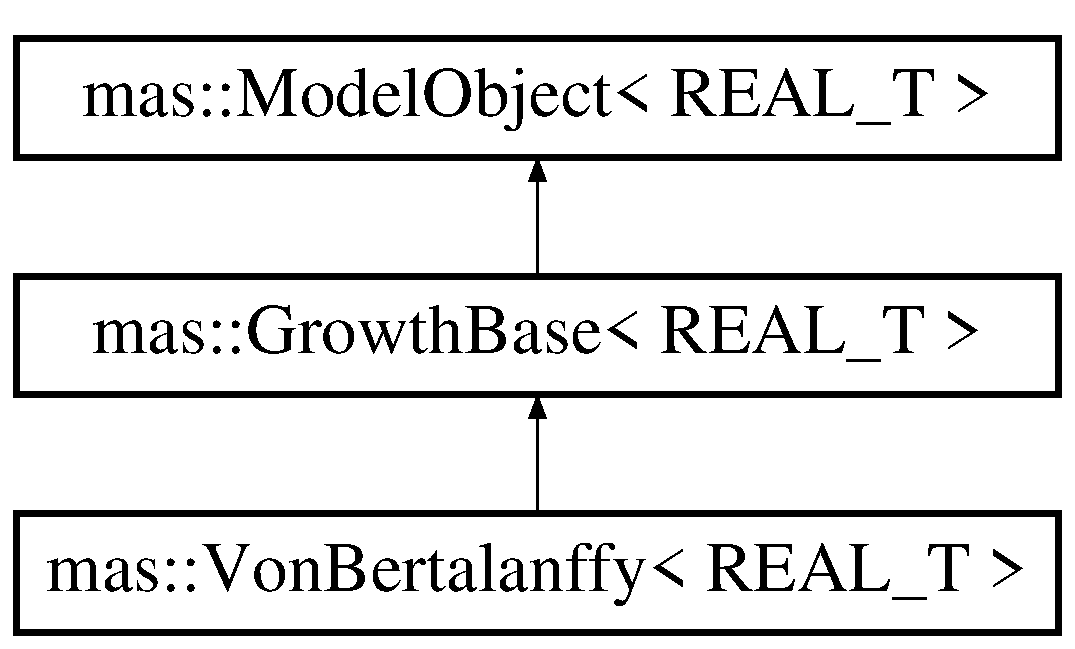
\includegraphics[height=3.000000cm]{structmas_1_1_von_bertalanffy}
\end{center}
\end{figure}
\subsection*{Public Types}
\begin{DoxyCompactItemize}
\item 
typedef \hyperlink{structmas_1_1_variable_trait}{Variable\-Trait}$<$ R\-E\-A\-L\-\_\-\-T $>$\\*
\-::\hyperlink{structmas_1_1_von_bertalanffy_a44edcdf23cc66a10c6744741588492b9}{variable} \hyperlink{structmas_1_1_von_bertalanffy_a44edcdf23cc66a10c6744741588492b9}{variable}
\end{DoxyCompactItemize}
\subsection*{Public Member Functions}
\begin{DoxyCompactItemize}
\item 
virtual const \hyperlink{structmas_1_1_von_bertalanffy_a44edcdf23cc66a10c6744741588492b9}{variable} \hyperlink{structmas_1_1_von_bertalanffy_ac89c031af93f2baf47d357bca9c37b6a}{Evaluate} (const \hyperlink{structmas_1_1_von_bertalanffy_a44edcdf23cc66a10c6744741588492b9}{variable} \&age, const int \&sex)
\item 
virtual const std\-::string \hyperlink{structmas_1_1_von_bertalanffy_a8d8c204940577c3b4e515baae839c15d}{Name} ()
\item 
virtual const std\-::string \hyperlink{structmas_1_1_von_bertalanffy_a1b579d133d8f9d068afec3b3a386ceec}{To\-J\-S\-O\-N\-String} ()
\item 
virtual std\-::string \hyperlink{structmas_1_1_von_bertalanffy_af301e548d6d3e9df5a2fc65132378195}{To\-String} ()
\end{DoxyCompactItemize}
\subsection*{Public Attributes}
\begin{DoxyCompactItemize}
\item 
\hyperlink{structmas_1_1_von_bertalanffy_a44edcdf23cc66a10c6744741588492b9}{variable} \hyperlink{structmas_1_1_von_bertalanffy_a6478a55daec32dd2e49104bda9207586}{k}
\item 
\hyperlink{structmas_1_1_von_bertalanffy_a44edcdf23cc66a10c6744741588492b9}{variable} \hyperlink{structmas_1_1_von_bertalanffy_a1c1c468cf32d014d16dcf8d9defccc46}{l\-\_\-inf}
\end{DoxyCompactItemize}


\subsection{Detailed Description}
\subsubsection*{template$<$typename R\-E\-A\-L\-\_\-\-T$>$struct mas\-::\-Von\-Bertalanffy$<$ R\-E\-A\-L\-\_\-\-T $>$}



Definition at line 78 of file Growth.\-hpp.



\subsection{Member Typedef Documentation}
\hypertarget{structmas_1_1_von_bertalanffy_a44edcdf23cc66a10c6744741588492b9}{\index{mas\-::\-Von\-Bertalanffy@{mas\-::\-Von\-Bertalanffy}!variable@{variable}}
\index{variable@{variable}!mas::VonBertalanffy@{mas\-::\-Von\-Bertalanffy}}
\subsubsection[{variable}]{\setlength{\rightskip}{0pt plus 5cm}template$<$typename R\-E\-A\-L\-\_\-\-T $>$ typedef {\bf Variable\-Trait}$<$R\-E\-A\-L\-\_\-\-T$>$\-::{\bf variable} {\bf mas\-::\-Von\-Bertalanffy}$<$ R\-E\-A\-L\-\_\-\-T $>$\-::{\bf variable}}}\label{structmas_1_1_von_bertalanffy_a44edcdf23cc66a10c6744741588492b9}


Definition at line 79 of file Growth.\-hpp.



\subsection{Member Function Documentation}
\hypertarget{structmas_1_1_von_bertalanffy_ac89c031af93f2baf47d357bca9c37b6a}{\index{mas\-::\-Von\-Bertalanffy@{mas\-::\-Von\-Bertalanffy}!Evaluate@{Evaluate}}
\index{Evaluate@{Evaluate}!mas::VonBertalanffy@{mas\-::\-Von\-Bertalanffy}}
\subsubsection[{Evaluate}]{\setlength{\rightskip}{0pt plus 5cm}template$<$typename R\-E\-A\-L\-\_\-\-T $>$ virtual const {\bf variable} {\bf mas\-::\-Von\-Bertalanffy}$<$ R\-E\-A\-L\-\_\-\-T $>$\-::Evaluate (
\begin{DoxyParamCaption}
\item[{const {\bf variable} \&}]{age, }
\item[{const int \&}]{sex}
\end{DoxyParamCaption}
)\hspace{0.3cm}{\ttfamily [inline]}, {\ttfamily [virtual]}}}\label{structmas_1_1_von_bertalanffy_ac89c031af93f2baf47d357bca9c37b6a}
Computes the length of a fish at age by sex.


\begin{DoxyParams}{Parameters}
{\em age} & \\
\hline
{\em sex} & \\
\hline
\end{DoxyParams}
\begin{DoxyReturn}{Returns}
length 
\end{DoxyReturn}


Implements \hyperlink{structmas_1_1_growth_base_a381e3400e22b2739830351acdf4689b5}{mas\-::\-Growth\-Base$<$ R\-E\-A\-L\-\_\-\-T $>$}.



Definition at line 83 of file Growth.\-hpp.

\hypertarget{structmas_1_1_von_bertalanffy_a8d8c204940577c3b4e515baae839c15d}{\index{mas\-::\-Von\-Bertalanffy@{mas\-::\-Von\-Bertalanffy}!Name@{Name}}
\index{Name@{Name}!mas::VonBertalanffy@{mas\-::\-Von\-Bertalanffy}}
\subsubsection[{Name}]{\setlength{\rightskip}{0pt plus 5cm}template$<$typename R\-E\-A\-L\-\_\-\-T $>$ virtual const std\-::string {\bf mas\-::\-Von\-Bertalanffy}$<$ R\-E\-A\-L\-\_\-\-T $>$\-::Name (
\begin{DoxyParamCaption}
{}
\end{DoxyParamCaption}
)\hspace{0.3cm}{\ttfamily [inline]}, {\ttfamily [virtual]}}}\label{structmas_1_1_von_bertalanffy_a8d8c204940577c3b4e515baae839c15d}


Reimplemented from \hyperlink{structmas_1_1_growth_base_a3645c79a5cd9ed606bcf2f381aef5259}{mas\-::\-Growth\-Base$<$ R\-E\-A\-L\-\_\-\-T $>$}.



Definition at line 88 of file Growth.\-hpp.

\hypertarget{structmas_1_1_von_bertalanffy_a1b579d133d8f9d068afec3b3a386ceec}{\index{mas\-::\-Von\-Bertalanffy@{mas\-::\-Von\-Bertalanffy}!To\-J\-S\-O\-N\-String@{To\-J\-S\-O\-N\-String}}
\index{To\-J\-S\-O\-N\-String@{To\-J\-S\-O\-N\-String}!mas::VonBertalanffy@{mas\-::\-Von\-Bertalanffy}}
\subsubsection[{To\-J\-S\-O\-N\-String}]{\setlength{\rightskip}{0pt plus 5cm}template$<$typename R\-E\-A\-L\-\_\-\-T $>$ virtual const std\-::string {\bf mas\-::\-Von\-Bertalanffy}$<$ R\-E\-A\-L\-\_\-\-T $>$\-::To\-J\-S\-O\-N\-String (
\begin{DoxyParamCaption}
{}
\end{DoxyParamCaption}
)\hspace{0.3cm}{\ttfamily [inline]}, {\ttfamily [virtual]}}}\label{structmas_1_1_von_bertalanffy_a1b579d133d8f9d068afec3b3a386ceec}


Reimplemented from \hyperlink{structmas_1_1_model_object_af40b3c89b11919fc5aea21dcf1cd027b}{mas\-::\-Model\-Object$<$ R\-E\-A\-L\-\_\-\-T $>$}.



Definition at line 92 of file Growth.\-hpp.

\hypertarget{structmas_1_1_von_bertalanffy_af301e548d6d3e9df5a2fc65132378195}{\index{mas\-::\-Von\-Bertalanffy@{mas\-::\-Von\-Bertalanffy}!To\-String@{To\-String}}
\index{To\-String@{To\-String}!mas::VonBertalanffy@{mas\-::\-Von\-Bertalanffy}}
\subsubsection[{To\-String}]{\setlength{\rightskip}{0pt plus 5cm}template$<$typename R\-E\-A\-L\-\_\-\-T $>$ virtual std\-::string {\bf mas\-::\-Von\-Bertalanffy}$<$ R\-E\-A\-L\-\_\-\-T $>$\-::To\-String (
\begin{DoxyParamCaption}
{}
\end{DoxyParamCaption}
)\hspace{0.3cm}{\ttfamily [inline]}, {\ttfamily [virtual]}}}\label{structmas_1_1_von_bertalanffy_af301e548d6d3e9df5a2fc65132378195}


Reimplemented from \hyperlink{structmas_1_1_model_object_a8eaf6c7c52e42ea8869aefa318358cb5}{mas\-::\-Model\-Object$<$ R\-E\-A\-L\-\_\-\-T $>$}.



Definition at line 110 of file Growth.\-hpp.



\subsection{Member Data Documentation}
\hypertarget{structmas_1_1_von_bertalanffy_a6478a55daec32dd2e49104bda9207586}{\index{mas\-::\-Von\-Bertalanffy@{mas\-::\-Von\-Bertalanffy}!k@{k}}
\index{k@{k}!mas::VonBertalanffy@{mas\-::\-Von\-Bertalanffy}}
\subsubsection[{k}]{\setlength{\rightskip}{0pt plus 5cm}template$<$typename R\-E\-A\-L\-\_\-\-T $>$ {\bf variable} {\bf mas\-::\-Von\-Bertalanffy}$<$ R\-E\-A\-L\-\_\-\-T $>$\-::k}}\label{structmas_1_1_von_bertalanffy_a6478a55daec32dd2e49104bda9207586}


Definition at line 80 of file Growth.\-hpp.

\hypertarget{structmas_1_1_von_bertalanffy_a1c1c468cf32d014d16dcf8d9defccc46}{\index{mas\-::\-Von\-Bertalanffy@{mas\-::\-Von\-Bertalanffy}!l\-\_\-inf@{l\-\_\-inf}}
\index{l\-\_\-inf@{l\-\_\-inf}!mas::VonBertalanffy@{mas\-::\-Von\-Bertalanffy}}
\subsubsection[{l\-\_\-inf}]{\setlength{\rightskip}{0pt plus 5cm}template$<$typename R\-E\-A\-L\-\_\-\-T $>$ {\bf variable} {\bf mas\-::\-Von\-Bertalanffy}$<$ R\-E\-A\-L\-\_\-\-T $>$\-::l\-\_\-inf}}\label{structmas_1_1_von_bertalanffy_a1c1c468cf32d014d16dcf8d9defccc46}


Definition at line 81 of file Growth.\-hpp.



The documentation for this struct was generated from the following file\-:\begin{DoxyCompactItemize}
\item 
/home/oppy/\-Net\-Beans\-Projects/mas/\hyperlink{_growth_8hpp}{Growth.\-hpp}\end{DoxyCompactItemize}

\hypertarget{structmas_1_1_von_bertalanffy_modified}{\section{mas\-:\-:Von\-Bertalanffy\-Modified$<$ R\-E\-A\-L\-\_\-\-T $>$ Struct Template Reference}
\label{structmas_1_1_von_bertalanffy_modified}\index{mas\-::\-Von\-Bertalanffy\-Modified$<$ R\-E\-A\-L\-\_\-\-T $>$@{mas\-::\-Von\-Bertalanffy\-Modified$<$ R\-E\-A\-L\-\_\-\-T $>$}}
}


{\ttfamily \#include $<$Growth.\-hpp$>$}

Inheritance diagram for mas\-:\-:Von\-Bertalanffy\-Modified$<$ R\-E\-A\-L\-\_\-\-T $>$\-:\begin{figure}[H]
\begin{center}
\leavevmode
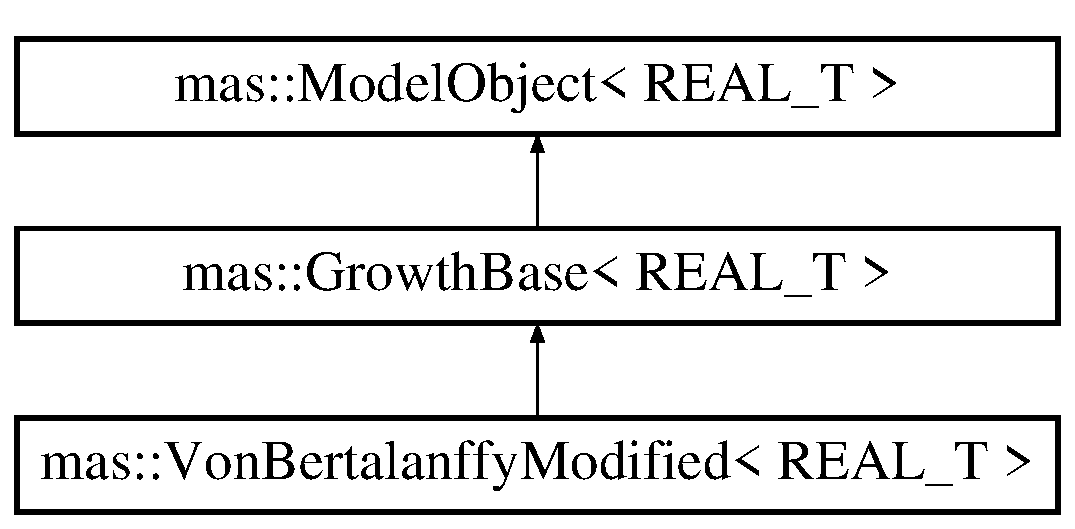
\includegraphics[height=3.000000cm]{structmas_1_1_von_bertalanffy_modified}
\end{center}
\end{figure}
\subsection*{Public Types}
\begin{DoxyCompactItemize}
\item 
typedef \hyperlink{structmas_1_1_variable_trait}{Variable\-Trait}$<$ R\-E\-A\-L\-\_\-\-T $>$\\*
\-::\hyperlink{structmas_1_1_von_bertalanffy_modified_af5a89449b12de884a01c34464ba2bae0}{variable} \hyperlink{structmas_1_1_von_bertalanffy_modified_af5a89449b12de884a01c34464ba2bae0}{variable}
\end{DoxyCompactItemize}
\subsection*{Public Member Functions}
\begin{DoxyCompactItemize}
\item 
virtual const \hyperlink{structmas_1_1_von_bertalanffy_modified_af5a89449b12de884a01c34464ba2bae0}{variable} \hyperlink{structmas_1_1_von_bertalanffy_modified_ac5e51a32119b7353bb32d64f440416c7}{Evaluate} (const \hyperlink{structmas_1_1_von_bertalanffy_modified_af5a89449b12de884a01c34464ba2bae0}{variable} \&age, const int \&sex)
\item 
virtual const std\-::string \hyperlink{structmas_1_1_von_bertalanffy_modified_a47465618fc2471ad0f47f94fe3974597}{To\-J\-S\-O\-N\-String} ()
\item 
virtual const std\-::string \hyperlink{structmas_1_1_von_bertalanffy_modified_a6c845df6e13d5219cd56614d323aaa79}{Name} ()
\item 
virtual std\-::string \hyperlink{structmas_1_1_von_bertalanffy_modified_a45e40092ed15953212d65c406908d708}{To\-String} ()
\end{DoxyCompactItemize}
\subsection*{Public Attributes}
\begin{DoxyCompactItemize}
\item 
\hyperlink{structmas_1_1_von_bertalanffy_modified_af5a89449b12de884a01c34464ba2bae0}{variable} \hyperlink{structmas_1_1_von_bertalanffy_modified_a2845686ae982422d40b571cb19712cc9}{lmin}
\item 
\hyperlink{structmas_1_1_von_bertalanffy_modified_af5a89449b12de884a01c34464ba2bae0}{variable} \hyperlink{structmas_1_1_von_bertalanffy_modified_a841b52d7c02054bb25516558f192a092}{lmax}
\item 
\hyperlink{structmas_1_1_von_bertalanffy_modified_af5a89449b12de884a01c34464ba2bae0}{variable} \hyperlink{structmas_1_1_von_bertalanffy_modified_a474caebe2c9277303d7bdba03101432c}{l\-\_\-inf}
\item 
\hyperlink{structmas_1_1_von_bertalanffy_modified_af5a89449b12de884a01c34464ba2bae0}{variable} \hyperlink{structmas_1_1_von_bertalanffy_modified_ac1ceb4a5dc583de01c35054eb5034f1d}{c}
\end{DoxyCompactItemize}


\subsection{Detailed Description}
\subsubsection*{template$<$typename R\-E\-A\-L\-\_\-\-T$>$struct mas\-::\-Von\-Bertalanffy\-Modified$<$ R\-E\-A\-L\-\_\-\-T $>$}



Definition at line 120 of file Growth.\-hpp.



\subsection{Member Typedef Documentation}
\hypertarget{structmas_1_1_von_bertalanffy_modified_af5a89449b12de884a01c34464ba2bae0}{\index{mas\-::\-Von\-Bertalanffy\-Modified@{mas\-::\-Von\-Bertalanffy\-Modified}!variable@{variable}}
\index{variable@{variable}!mas::VonBertalanffyModified@{mas\-::\-Von\-Bertalanffy\-Modified}}
\subsubsection[{variable}]{\setlength{\rightskip}{0pt plus 5cm}template$<$typename R\-E\-A\-L\-\_\-\-T $>$ typedef {\bf Variable\-Trait}$<$R\-E\-A\-L\-\_\-\-T$>$\-::{\bf variable} {\bf mas\-::\-Von\-Bertalanffy\-Modified}$<$ R\-E\-A\-L\-\_\-\-T $>$\-::{\bf variable}}}\label{structmas_1_1_von_bertalanffy_modified_af5a89449b12de884a01c34464ba2bae0}


Definition at line 121 of file Growth.\-hpp.



\subsection{Member Function Documentation}
\hypertarget{structmas_1_1_von_bertalanffy_modified_ac5e51a32119b7353bb32d64f440416c7}{\index{mas\-::\-Von\-Bertalanffy\-Modified@{mas\-::\-Von\-Bertalanffy\-Modified}!Evaluate@{Evaluate}}
\index{Evaluate@{Evaluate}!mas::VonBertalanffyModified@{mas\-::\-Von\-Bertalanffy\-Modified}}
\subsubsection[{Evaluate}]{\setlength{\rightskip}{0pt plus 5cm}template$<$typename R\-E\-A\-L\-\_\-\-T $>$ virtual const {\bf variable} {\bf mas\-::\-Von\-Bertalanffy\-Modified}$<$ R\-E\-A\-L\-\_\-\-T $>$\-::Evaluate (
\begin{DoxyParamCaption}
\item[{const {\bf variable} \&}]{age, }
\item[{const int \&}]{sex}
\end{DoxyParamCaption}
)\hspace{0.3cm}{\ttfamily [inline]}, {\ttfamily [virtual]}}}\label{structmas_1_1_von_bertalanffy_modified_ac5e51a32119b7353bb32d64f440416c7}
Computes the length of a fish at age by sex.


\begin{DoxyParams}{Parameters}
{\em age} & \\
\hline
{\em sex} & \\
\hline
\end{DoxyParams}
\begin{DoxyReturn}{Returns}
length 
\end{DoxyReturn}


Implements \hyperlink{structmas_1_1_growth_base_a381e3400e22b2739830351acdf4689b5}{mas\-::\-Growth\-Base$<$ R\-E\-A\-L\-\_\-\-T $>$}.



Definition at line 127 of file Growth.\-hpp.

\hypertarget{structmas_1_1_von_bertalanffy_modified_a6c845df6e13d5219cd56614d323aaa79}{\index{mas\-::\-Von\-Bertalanffy\-Modified@{mas\-::\-Von\-Bertalanffy\-Modified}!Name@{Name}}
\index{Name@{Name}!mas::VonBertalanffyModified@{mas\-::\-Von\-Bertalanffy\-Modified}}
\subsubsection[{Name}]{\setlength{\rightskip}{0pt plus 5cm}template$<$typename R\-E\-A\-L\-\_\-\-T $>$ virtual const std\-::string {\bf mas\-::\-Von\-Bertalanffy\-Modified}$<$ R\-E\-A\-L\-\_\-\-T $>$\-::Name (
\begin{DoxyParamCaption}
{}
\end{DoxyParamCaption}
)\hspace{0.3cm}{\ttfamily [inline]}, {\ttfamily [virtual]}}}\label{structmas_1_1_von_bertalanffy_modified_a6c845df6e13d5219cd56614d323aaa79}


Reimplemented from \hyperlink{structmas_1_1_growth_base_a3645c79a5cd9ed606bcf2f381aef5259}{mas\-::\-Growth\-Base$<$ R\-E\-A\-L\-\_\-\-T $>$}.



Definition at line 153 of file Growth.\-hpp.

\hypertarget{structmas_1_1_von_bertalanffy_modified_a47465618fc2471ad0f47f94fe3974597}{\index{mas\-::\-Von\-Bertalanffy\-Modified@{mas\-::\-Von\-Bertalanffy\-Modified}!To\-J\-S\-O\-N\-String@{To\-J\-S\-O\-N\-String}}
\index{To\-J\-S\-O\-N\-String@{To\-J\-S\-O\-N\-String}!mas::VonBertalanffyModified@{mas\-::\-Von\-Bertalanffy\-Modified}}
\subsubsection[{To\-J\-S\-O\-N\-String}]{\setlength{\rightskip}{0pt plus 5cm}template$<$typename R\-E\-A\-L\-\_\-\-T $>$ virtual const std\-::string {\bf mas\-::\-Von\-Bertalanffy\-Modified}$<$ R\-E\-A\-L\-\_\-\-T $>$\-::To\-J\-S\-O\-N\-String (
\begin{DoxyParamCaption}
{}
\end{DoxyParamCaption}
)\hspace{0.3cm}{\ttfamily [inline]}, {\ttfamily [virtual]}}}\label{structmas_1_1_von_bertalanffy_modified_a47465618fc2471ad0f47f94fe3974597}


Reimplemented from \hyperlink{structmas_1_1_model_object_af40b3c89b11919fc5aea21dcf1cd027b}{mas\-::\-Model\-Object$<$ R\-E\-A\-L\-\_\-\-T $>$}.



Definition at line 133 of file Growth.\-hpp.

\hypertarget{structmas_1_1_von_bertalanffy_modified_a45e40092ed15953212d65c406908d708}{\index{mas\-::\-Von\-Bertalanffy\-Modified@{mas\-::\-Von\-Bertalanffy\-Modified}!To\-String@{To\-String}}
\index{To\-String@{To\-String}!mas::VonBertalanffyModified@{mas\-::\-Von\-Bertalanffy\-Modified}}
\subsubsection[{To\-String}]{\setlength{\rightskip}{0pt plus 5cm}template$<$typename R\-E\-A\-L\-\_\-\-T $>$ virtual std\-::string {\bf mas\-::\-Von\-Bertalanffy\-Modified}$<$ R\-E\-A\-L\-\_\-\-T $>$\-::To\-String (
\begin{DoxyParamCaption}
{}
\end{DoxyParamCaption}
)\hspace{0.3cm}{\ttfamily [inline]}, {\ttfamily [virtual]}}}\label{structmas_1_1_von_bertalanffy_modified_a45e40092ed15953212d65c406908d708}


Reimplemented from \hyperlink{structmas_1_1_model_object_a8eaf6c7c52e42ea8869aefa318358cb5}{mas\-::\-Model\-Object$<$ R\-E\-A\-L\-\_\-\-T $>$}.



Definition at line 157 of file Growth.\-hpp.



\subsection{Member Data Documentation}
\hypertarget{structmas_1_1_von_bertalanffy_modified_ac1ceb4a5dc583de01c35054eb5034f1d}{\index{mas\-::\-Von\-Bertalanffy\-Modified@{mas\-::\-Von\-Bertalanffy\-Modified}!c@{c}}
\index{c@{c}!mas::VonBertalanffyModified@{mas\-::\-Von\-Bertalanffy\-Modified}}
\subsubsection[{c}]{\setlength{\rightskip}{0pt plus 5cm}template$<$typename R\-E\-A\-L\-\_\-\-T $>$ {\bf variable} {\bf mas\-::\-Von\-Bertalanffy\-Modified}$<$ R\-E\-A\-L\-\_\-\-T $>$\-::c}}\label{structmas_1_1_von_bertalanffy_modified_ac1ceb4a5dc583de01c35054eb5034f1d}


Definition at line 125 of file Growth.\-hpp.

\hypertarget{structmas_1_1_von_bertalanffy_modified_a474caebe2c9277303d7bdba03101432c}{\index{mas\-::\-Von\-Bertalanffy\-Modified@{mas\-::\-Von\-Bertalanffy\-Modified}!l\-\_\-inf@{l\-\_\-inf}}
\index{l\-\_\-inf@{l\-\_\-inf}!mas::VonBertalanffyModified@{mas\-::\-Von\-Bertalanffy\-Modified}}
\subsubsection[{l\-\_\-inf}]{\setlength{\rightskip}{0pt plus 5cm}template$<$typename R\-E\-A\-L\-\_\-\-T $>$ {\bf variable} {\bf mas\-::\-Von\-Bertalanffy\-Modified}$<$ R\-E\-A\-L\-\_\-\-T $>$\-::l\-\_\-inf}}\label{structmas_1_1_von_bertalanffy_modified_a474caebe2c9277303d7bdba03101432c}


Definition at line 124 of file Growth.\-hpp.

\hypertarget{structmas_1_1_von_bertalanffy_modified_a841b52d7c02054bb25516558f192a092}{\index{mas\-::\-Von\-Bertalanffy\-Modified@{mas\-::\-Von\-Bertalanffy\-Modified}!lmax@{lmax}}
\index{lmax@{lmax}!mas::VonBertalanffyModified@{mas\-::\-Von\-Bertalanffy\-Modified}}
\subsubsection[{lmax}]{\setlength{\rightskip}{0pt plus 5cm}template$<$typename R\-E\-A\-L\-\_\-\-T $>$ {\bf variable} {\bf mas\-::\-Von\-Bertalanffy\-Modified}$<$ R\-E\-A\-L\-\_\-\-T $>$\-::lmax}}\label{structmas_1_1_von_bertalanffy_modified_a841b52d7c02054bb25516558f192a092}


Definition at line 123 of file Growth.\-hpp.

\hypertarget{structmas_1_1_von_bertalanffy_modified_a2845686ae982422d40b571cb19712cc9}{\index{mas\-::\-Von\-Bertalanffy\-Modified@{mas\-::\-Von\-Bertalanffy\-Modified}!lmin@{lmin}}
\index{lmin@{lmin}!mas::VonBertalanffyModified@{mas\-::\-Von\-Bertalanffy\-Modified}}
\subsubsection[{lmin}]{\setlength{\rightskip}{0pt plus 5cm}template$<$typename R\-E\-A\-L\-\_\-\-T $>$ {\bf variable} {\bf mas\-::\-Von\-Bertalanffy\-Modified}$<$ R\-E\-A\-L\-\_\-\-T $>$\-::lmin}}\label{structmas_1_1_von_bertalanffy_modified_a2845686ae982422d40b571cb19712cc9}


Definition at line 122 of file Growth.\-hpp.



The documentation for this struct was generated from the following file\-:\begin{DoxyCompactItemize}
\item 
/home/oppy/\-Net\-Beans\-Projects/mas/\hyperlink{_growth_8hpp}{Growth.\-hpp}\end{DoxyCompactItemize}

\hypertarget{classmas_1_1_wait_variable}{\section{mas\-:\-:Wait\-Variable Class Reference}
\label{classmas_1_1_wait_variable}\index{mas\-::\-Wait\-Variable@{mas\-::\-Wait\-Variable}}
}


{\ttfamily \#include $<$Thread\-Pool.\-hpp$>$}

\subsection*{Public Member Functions}
\begin{DoxyCompactItemize}
\item 
\hyperlink{classmas_1_1_wait_variable_a8d3b80a432c00f555cf5d0604655062e}{Wait\-Variable} ()
\end{DoxyCompactItemize}
\subsection*{Friends}
\begin{DoxyCompactItemize}
\item 
class \hyperlink{classmas_1_1_wait_variable_a5d97748be7d69dcc44ef551ea35ef20f}{Thread\-Pool}
\end{DoxyCompactItemize}


\subsection{Detailed Description}


Definition at line 95 of file Thread\-Pool.\-hpp.



\subsection{Constructor \& Destructor Documentation}
\hypertarget{classmas_1_1_wait_variable_a8d3b80a432c00f555cf5d0604655062e}{\index{mas\-::\-Wait\-Variable@{mas\-::\-Wait\-Variable}!Wait\-Variable@{Wait\-Variable}}
\index{Wait\-Variable@{Wait\-Variable}!mas::WaitVariable@{mas\-::\-Wait\-Variable}}
\subsubsection[{Wait\-Variable}]{\setlength{\rightskip}{0pt plus 5cm}mas\-::\-Wait\-Variable\-::\-Wait\-Variable (
\begin{DoxyParamCaption}
{}
\end{DoxyParamCaption}
)\hspace{0.3cm}{\ttfamily [inline]}}}\label{classmas_1_1_wait_variable_a8d3b80a432c00f555cf5d0604655062e}


Definition at line 110 of file Thread\-Pool.\-hpp.



\subsection{Friends And Related Function Documentation}
\hypertarget{classmas_1_1_wait_variable_a5d97748be7d69dcc44ef551ea35ef20f}{\index{mas\-::\-Wait\-Variable@{mas\-::\-Wait\-Variable}!Thread\-Pool@{Thread\-Pool}}
\index{Thread\-Pool@{Thread\-Pool}!mas::WaitVariable@{mas\-::\-Wait\-Variable}}
\subsubsection[{Thread\-Pool}]{\setlength{\rightskip}{0pt plus 5cm}friend class {\bf Thread\-Pool}\hspace{0.3cm}{\ttfamily [friend]}}}\label{classmas_1_1_wait_variable_a5d97748be7d69dcc44ef551ea35ef20f}


Definition at line 96 of file Thread\-Pool.\-hpp.



The documentation for this class was generated from the following file\-:\begin{DoxyCompactItemize}
\item 
/home/oppy/\-Net\-Beans\-Projects/mas/\hyperlink{_thread_pool_8hpp}{Thread\-Pool.\-hpp}\end{DoxyCompactItemize}

\chapter{File Documentation}
\hypertarget{_area_8hpp}{\section{/home/oppy/\-Net\-Beans\-Projects/mas/\-Area.hpp File Reference}
\label{_area_8hpp}\index{/home/oppy/\-Net\-Beans\-Projects/mas/\-Area.\-hpp@{/home/oppy/\-Net\-Beans\-Projects/mas/\-Area.\-hpp}}
}
{\ttfamily \#include \char`\"{}Recruitment.\-hpp\char`\"{}}\\*
{\ttfamily \#include \char`\"{}Mortality.\-hpp\char`\"{}}\\*
{\ttfamily \#include \char`\"{}Growth.\-hpp\char`\"{}}\\*
{\ttfamily \#include \char`\"{}Fecundity.\-hpp\char`\"{}}\\*
{\ttfamily \#include \char`\"{}Selectivity.\-hpp\char`\"{}}\\*
{\ttfamily \#include \char`\"{}Fleet.\-hpp\char`\"{}}\\*
{\ttfamily \#include \char`\"{}Survey.\-hpp\char`\"{}}\\*
\subsection*{Classes}
\begin{DoxyCompactItemize}
\item 
struct \hyperlink{structmas_1_1_area}{mas\-::\-Area$<$ R\-E\-A\-L\-\_\-\-T $>$}
\end{DoxyCompactItemize}
\subsection*{Namespaces}
\begin{DoxyCompactItemize}
\item 
\hyperlink{namespacemas}{mas}
\end{DoxyCompactItemize}
\subsection*{Functions}
\begin{DoxyCompactItemize}
\item 
{\footnotesize template$<$typename R\-E\-A\-L\-\_\-\-T $>$ }\\std\-::ostream \& \hyperlink{namespacemas_aba0d00c366d7334ce6343f8011c2316c}{mas\-::operator$<$$<$} (std\-::ostream \&out, const \hyperlink{structmas_1_1_area}{mas\-::\-Area}$<$ R\-E\-A\-L\-\_\-\-T $>$ \&area)
\end{DoxyCompactItemize}

\hypertarget{_common_8hpp}{\section{/home/oppy/\-Net\-Beans\-Projects/mas/\-Common.hpp File Reference}
\label{_common_8hpp}\index{/home/oppy/\-Net\-Beans\-Projects/mas/\-Common.\-hpp@{/home/oppy/\-Net\-Beans\-Projects/mas/\-Common.\-hpp}}
}
{\ttfamily \#include \char`\"{}third\-\_\-party/\-A\-T\-L/\-A\-T\-L.\-hpp\char`\"{}}\\*
{\ttfamily \#include $<$vector$>$}\\*
{\ttfamily \#include $<$map$>$}\\*
{\ttfamily \#include $<$utility$>$}\\*
{\ttfamily \#include $<$tuple$>$}\\*
\subsection*{Classes}
\begin{DoxyCompactItemize}
\item 
struct \hyperlink{structmas_1_1_variable_trait}{mas\-::\-Variable\-Trait$<$ R\-E\-A\-L\-\_\-\-T $>$}
\item 
struct \hyperlink{structmas_1_1_model_object}{mas\-::\-Model\-Object$<$ R\-E\-A\-L\-\_\-\-T $>$}
\item 
struct \hyperlink{structmas_1_1_data_object}{mas\-::\-Data\-Object$<$ R\-E\-A\-L\-\_\-\-T $>$}
\item 
struct \hyperlink{structmas_1_1_initial_numbers}{mas\-::\-Initial\-Numbers$<$ R\-E\-A\-L\-\_\-\-T $>$}
\end{DoxyCompactItemize}
\subsection*{Namespaces}
\begin{DoxyCompactItemize}
\item 
\hyperlink{namespacemas}{mas}
\end{DoxyCompactItemize}
\subsection*{Enumerations}
\begin{DoxyCompactItemize}
\item 
enum \hyperlink{namespacemas_a7e15982b9bc2fc35b571bceea4f85a6b}{mas\-::\-Data\-Units} \{ \\*
\hyperlink{namespacemas_a7e15982b9bc2fc35b571bceea4f85a6ba24ba23cbe986514f8d11f362fa3930fa}{mas\-::\-M\-T} = 0, 
\hyperlink{namespacemas_a7e15982b9bc2fc35b571bceea4f85a6ba717fa60c06e10278cbb6af9c89846204}{mas\-::\-K\-G}, 
\hyperlink{namespacemas_a7e15982b9bc2fc35b571bceea4f85a6ba83f219df1658ee24c04b5aae8be3e9b4}{mas\-::\-L\-B\-S}, 
\hyperlink{namespacemas_a7e15982b9bc2fc35b571bceea4f85a6ba9f88b87b3a94ede2bf085ae719c5d264}{mas\-::\-I\-T}, 
\\*
\hyperlink{namespacemas_a7e15982b9bc2fc35b571bceea4f85a6baae97c65d42e8b626638c1de602c1a666}{mas\-::\-N\-U\-M\-B\-E\-R\-S}, 
\hyperlink{namespacemas_a7e15982b9bc2fc35b571bceea4f85a6ba3ad4cc78219ff2bb2190866ab0bfe269}{mas\-::\-N\-A}
 \}
\item 
enum \hyperlink{namespacemas_a011cdbd288b3370538941f20c874de27}{mas\-::\-Data\-Object\-Type} \{ \\*
\hyperlink{namespacemas_a011cdbd288b3370538941f20c874de27a91e0c09d0a7c65d6d0d871d57c069354}{mas\-::\-C\-A\-T\-C\-H\-\_\-\-B\-I\-O\-M\-A\-S\-S} = 0, 
\hyperlink{namespacemas_a011cdbd288b3370538941f20c874de27a8835020daf124e9224f6b47bcac9fc25}{mas\-::\-C\-A\-T\-C\-H\-\_\-\-P\-R\-O\-P\-O\-R\-T\-I\-O\-N\-\_\-\-A\-T\-\_\-\-A\-G\-E\-\_\-\-N}, 
\hyperlink{namespacemas_a011cdbd288b3370538941f20c874de27ac1ac07dc7b7ffd0749afe5212fc072d6}{mas\-::\-C\-A\-T\-C\-H\-\_\-\-P\-R\-O\-P\-O\-R\-T\-I\-O\-N\-\_\-\-A\-T\-\_\-\-A\-G\-E}, 
\hyperlink{namespacemas_a011cdbd288b3370538941f20c874de27a9d0db3c48ce40586e86c9c8e6958999c}{mas\-::\-C\-A\-T\-C\-H\-\_\-\-P\-R\-O\-P\-O\-R\-T\-I\-O\-N\-\_\-\-A\-T\-\_\-\-L\-E\-N\-G\-T\-H\-\_\-\-N}, 
\\*
\hyperlink{namespacemas_a011cdbd288b3370538941f20c874de27a13505e72234d2fba94fda6c2ce2a8910}{mas\-::\-C\-A\-T\-C\-H\-\_\-\-P\-R\-O\-P\-O\-R\-T\-I\-O\-N\-\_\-\-A\-T\-\_\-\-L\-E\-N\-G\-T\-H}, 
\hyperlink{namespacemas_a011cdbd288b3370538941f20c874de27a9477c55e49a0032670dfc591cd8531b2}{mas\-::\-C\-A\-T\-C\-H\-\_\-\-M\-E\-A\-N\-\_\-\-S\-I\-Z\-E\-\_\-\-A\-T\-\_\-\-A\-G\-E}, 
\hyperlink{namespacemas_a011cdbd288b3370538941f20c874de27ac327e723f8878231018c79af30448e6e}{mas\-::\-C\-A\-T\-C\-H\-\_\-\-M\-E\-A\-N\-\_\-\-W\-E\-I\-G\-H\-T\-\_\-\-A\-T\-\_\-\-A\-G\-E}, 
\hyperlink{namespacemas_a011cdbd288b3370538941f20c874de27a032bff9d6483e4a2e6a2bcf073ee8964}{mas\-::\-S\-U\-R\-V\-E\-Y\-\_\-\-B\-I\-O\-M\-A\-S\-S}, 
\\*
\hyperlink{namespacemas_a011cdbd288b3370538941f20c874de27a22f0f2b5da0c3a58f1c1a5feb4beff39}{mas\-::\-S\-U\-R\-V\-E\-Y\-\_\-\-P\-R\-O\-P\-O\-R\-T\-I\-O\-N\-\_\-\-A\-T\-\_\-\-A\-G\-E\-\_\-\-N}, 
\hyperlink{namespacemas_a011cdbd288b3370538941f20c874de27a0c11c6edfb00da9683356535a42d38c5}{mas\-::\-S\-U\-R\-V\-E\-Y\-\_\-\-P\-R\-O\-P\-O\-R\-T\-I\-O\-N\-\_\-\-A\-T\-\_\-\-A\-G\-E}, 
\hyperlink{namespacemas_a011cdbd288b3370538941f20c874de27a6799a1bbd7edffcddb12261c10ac6b8e}{mas\-::\-S\-U\-R\-V\-E\-Y\-\_\-\-P\-R\-O\-P\-O\-R\-T\-I\-O\-N\-\_\-\-A\-T\-\_\-\-L\-E\-N\-G\-T\-H\-\_\-\-N}, 
\hyperlink{namespacemas_a011cdbd288b3370538941f20c874de27a9679432b755bbda09adbb607c6eb4bcf}{mas\-::\-S\-U\-R\-V\-E\-Y\-\_\-\-P\-R\-O\-P\-O\-R\-T\-I\-O\-N\-\_\-\-A\-T\-\_\-\-L\-E\-N\-G\-T\-H}, 
\\*
\hyperlink{namespacemas_a011cdbd288b3370538941f20c874de27a3a5ef4509b5e77ffb2236d210e8a0f63}{mas\-::\-S\-U\-R\-V\-E\-Y\-\_\-\-M\-E\-A\-N\-\_\-\-S\-I\-Z\-E\-\_\-\-A\-T\-\_\-\-A\-G\-E}, 
\hyperlink{namespacemas_a011cdbd288b3370538941f20c874de27a1b8b664cf0211661b3cd2f5be86f19c5}{mas\-::\-S\-U\-R\-V\-E\-Y\-\_\-\-M\-E\-A\-N\-\_\-\-W\-E\-I\-G\-H\-T\-\_\-\-A\-T\-\_\-\-A\-G\-E}, 
\hyperlink{namespacemas_a011cdbd288b3370538941f20c874de27a5f6aa68de41891cc166f7edfc0c698b8}{mas\-::\-U\-N\-K\-N\-O\-W\-N}
 \}
\item 
enum \hyperlink{namespacemas_a177aaabcef4ec0c3f390a7c9f6ad563b}{mas\-::\-Fish\-Sex\-Type} \{ \hyperlink{namespacemas_a177aaabcef4ec0c3f390a7c9f6ad563ba4d0d21563331ebb4e3dcc56d8b5ec075}{mas\-::\-M\-A\-L\-E} = 0, 
\hyperlink{namespacemas_a177aaabcef4ec0c3f390a7c9f6ad563bacec7bc3874eee9c96cf1602b10651661}{mas\-::\-F\-E\-M\-A\-L\-E}, 
\hyperlink{namespacemas_a177aaabcef4ec0c3f390a7c9f6ad563ba6afb238d6c6138b53f11ec1b44e92417}{mas\-::\-U\-N\-D\-I\-F\-F\-E\-R\-E\-N\-T\-I\-A\-T\-E\-D}
 \}
\end{DoxyCompactItemize}
\subsection*{Functions}
\begin{DoxyCompactItemize}
\item 
std\-::ofstream \hyperlink{namespacemas_a54c9771e0c0b38688aa18475d3644319}{mas\-::mas\-\_\-log} (\char`\"{}mas.\-log\char`\"{})
\item 
{\footnotesize template$<$typename T $>$ }\\std\-::ostream \& \hyperlink{namespacemas_a798fc16eee04e2aeb2a546ab94f0791c}{mas\-::operator$<$$<$} (std\-::ostream \&out, const Model\-Object$<$ T $>$ \&model)
\item 
{\footnotesize template$<$typename T $>$ }\\std\-::ostream \& \hyperlink{namespacemas_a66ca3dc24d0031abac59251aae309c3e}{mas\-::operator$<$$<$} (std\-::ostream \&out, \hyperlink{structmas_1_1_data_object}{mas\-::\-Data\-Object}$<$ T $>$ \&data\-\_\-object)
\item 
{\footnotesize template$<$typename T $>$ }\\T \hyperlink{namespacemas_aeee9d6c296b5c135169fb0fc3bbc399e}{mas\-::\-String\-To\-Number} (const std\-::string \&Text)
\end{DoxyCompactItemize}

\hypertarget{_fecundity_8hpp}{\section{/home/oppy/\-Net\-Beans\-Projects/mas/\-Fecundity.hpp File Reference}
\label{_fecundity_8hpp}\index{/home/oppy/\-Net\-Beans\-Projects/mas/\-Fecundity.\-hpp@{/home/oppy/\-Net\-Beans\-Projects/mas/\-Fecundity.\-hpp}}
}
{\ttfamily \#include \char`\"{}Common.\-hpp\char`\"{}}\\*
\subsection*{Classes}
\begin{DoxyCompactItemize}
\item 
struct \hyperlink{structmas_1_1_fecundity_base}{mas\-::\-Fecundity\-Base$<$ R\-E\-A\-L\-\_\-\-T $>$}
\item 
struct \hyperlink{structmas_1_1_logistic_fec}{mas\-::\-Logistic\-Fec$<$ R\-E\-A\-L\-\_\-\-T $>$}
\item 
struct \hyperlink{structmas_1_1_double_logistic_fec}{mas\-::\-Double\-Logistic\-Fec$<$ R\-E\-A\-L\-\_\-\-T $>$}
\end{DoxyCompactItemize}
\subsection*{Namespaces}
\begin{DoxyCompactItemize}
\item 
\hyperlink{namespacemas}{mas}
\end{DoxyCompactItemize}

\hypertarget{_fleet_8hpp}{\section{/home/oppy/\-Net\-Beans\-Projects/mas/\-Fleet.hpp File Reference}
\label{_fleet_8hpp}\index{/home/oppy/\-Net\-Beans\-Projects/mas/\-Fleet.\-hpp@{/home/oppy/\-Net\-Beans\-Projects/mas/\-Fleet.\-hpp}}
}
{\ttfamily \#include $<$unordered\-\_\-set$>$}\\*
{\ttfamily \#include \char`\"{}Common.\-hpp\char`\"{}}\\*
{\ttfamily \#include \char`\"{}Selectivity.\-hpp\char`\"{}}\\*
{\ttfamily \#include \char`\"{}Area.\-hpp\char`\"{}}\\*
{\ttfamily \#include \char`\"{}N\-L\-L\-Components.\-hpp\char`\"{}}\\*
\subsection*{Classes}
\begin{DoxyCompactItemize}
\item 
struct \hyperlink{structmas_1_1_fleet}{mas\-::\-Fleet$<$ R\-E\-A\-L\-\_\-\-T $>$}
\end{DoxyCompactItemize}
\subsection*{Namespaces}
\begin{DoxyCompactItemize}
\item 
\hyperlink{namespacemas}{mas}
\end{DoxyCompactItemize}
\subsection*{Functions}
\begin{DoxyCompactItemize}
\item 
{\footnotesize template$<$typename R\-E\-A\-L\-\_\-\-T $>$ }\\std\-::ostream \& \hyperlink{namespacemas_aa20a850225fc4b2869aaeb534692a778}{mas\-::operator$<$$<$} (std\-::ostream \&out, const \hyperlink{structmas_1_1_fleet}{mas\-::\-Fleet}$<$ R\-E\-A\-L\-\_\-\-T $>$ \&fleet)
\end{DoxyCompactItemize}

\hypertarget{_forcast_8hpp}{\section{/home/oppy/\-Net\-Beans\-Projects/mas/\-Forcast.hpp File Reference}
\label{_forcast_8hpp}\index{/home/oppy/\-Net\-Beans\-Projects/mas/\-Forcast.\-hpp@{/home/oppy/\-Net\-Beans\-Projects/mas/\-Forcast.\-hpp}}
}
\subsection*{Classes}
\begin{DoxyCompactItemize}
\item 
class \hyperlink{classmas_1_1_forecast_base}{mas\-::\-Forecast\-Base$<$ R\-E\-A\-L\-\_\-\-T $>$}
\item 
class \hyperlink{classmas_1_1_age_pro}{mas\-::\-Age\-Pro$<$ T $>$}
\end{DoxyCompactItemize}
\subsection*{Namespaces}
\begin{DoxyCompactItemize}
\item 
\hyperlink{namespacemas}{mas}
\end{DoxyCompactItemize}

\hypertarget{_growth_8hpp}{\section{/home/oppy/\-Net\-Beans\-Projects/mas/\-Growth.hpp File Reference}
\label{_growth_8hpp}\index{/home/oppy/\-Net\-Beans\-Projects/mas/\-Growth.\-hpp@{/home/oppy/\-Net\-Beans\-Projects/mas/\-Growth.\-hpp}}
}
{\ttfamily \#include \char`\"{}Common.\-hpp\char`\"{}}\\*
\subsection*{Classes}
\begin{DoxyCompactItemize}
\item 
struct \hyperlink{structmas_1_1_growth_base}{mas\-::\-Growth\-Base$<$ R\-E\-A\-L\-\_\-\-T $>$}
\item 
struct \hyperlink{structmas_1_1_von_bertalanffy}{mas\-::\-Von\-Bertalanffy$<$ R\-E\-A\-L\-\_\-\-T $>$}
\item 
struct \hyperlink{structmas_1_1_von_bertalanffy_modified}{mas\-::\-Von\-Bertalanffy\-Modified$<$ R\-E\-A\-L\-\_\-\-T $>$}
\item 
struct \hyperlink{structmas_1_1_schnute_case_i}{mas\-::\-Schnute\-Case\-I$<$ R\-E\-A\-L\-\_\-\-T $>$}
\item 
struct \hyperlink{structmas_1_1_schnute_case_i_i}{mas\-::\-Schnute\-Case\-I\-I$<$ R\-E\-A\-L\-\_\-\-T $>$}
\item 
struct \hyperlink{structmas_1_1_schnute_case_i_i_i}{mas\-::\-Schnute\-Case\-I\-I\-I$<$ R\-E\-A\-L\-\_\-\-T $>$}
\item 
struct \hyperlink{structmas_1_1_schnute_case_i_v}{mas\-::\-Schnute\-Case\-I\-V$<$ R\-E\-A\-L\-\_\-\-T $>$}
\end{DoxyCompactItemize}
\subsection*{Namespaces}
\begin{DoxyCompactItemize}
\item 
\hyperlink{namespacemas}{mas}
\end{DoxyCompactItemize}

\hypertarget{_harvest_control_rule_8hpp}{\section{/home/oppy/\-Net\-Beans\-Projects/mas/\-Harvest\-Control\-Rule.hpp File Reference}
\label{_harvest_control_rule_8hpp}\index{/home/oppy/\-Net\-Beans\-Projects/mas/\-Harvest\-Control\-Rule.\-hpp@{/home/oppy/\-Net\-Beans\-Projects/mas/\-Harvest\-Control\-Rule.\-hpp}}
}
{\ttfamily \#include \char`\"{}Common.\-hpp\char`\"{}}\\*
{\ttfamily \#include \char`\"{}Fleet.\-hpp\char`\"{}}\\*
\subsection*{Classes}
\begin{DoxyCompactItemize}
\item 
struct \hyperlink{structmas_1_1_area_population_info}{mas\-::\-Area\-Population\-Info$<$ R\-E\-A\-L\-\_\-\-T $>$}
\item 
struct \hyperlink{structmas_1_1_h_c_r_base}{mas\-::\-H\-C\-R\-Base$<$ R\-E\-A\-L\-\_\-\-T $>$}
\item 
struct \hyperlink{structmas_1_1_n_p_f_m_c___tier3___h_c_r}{mas\-::\-N\-P\-F\-M\-C\-\_\-\-Tier3\-\_\-\-H\-C\-R$<$ R\-E\-A\-L\-\_\-\-T $>$}
\item 
struct \hyperlink{structmas_1_1_p_f_m_c___h_c_r}{mas\-::\-P\-F\-M\-C\-\_\-\-H\-C\-R$<$ R\-E\-A\-L\-\_\-\-T $>$}
\end{DoxyCompactItemize}
\subsection*{Namespaces}
\begin{DoxyCompactItemize}
\item 
\hyperlink{namespacemas}{mas}
\end{DoxyCompactItemize}

\hypertarget{_information_8hpp}{\section{/home/oppy/\-Net\-Beans\-Projects/mas/\-Information.hpp File Reference}
\label{_information_8hpp}\index{/home/oppy/\-Net\-Beans\-Projects/mas/\-Information.\-hpp@{/home/oppy/\-Net\-Beans\-Projects/mas/\-Information.\-hpp}}
}
{\ttfamily \#include \char`\"{}Common.\-hpp\char`\"{}}\\*
{\ttfamily \#include \char`\"{}Area.\-hpp\char`\"{}}\\*
{\ttfamily \#include \char`\"{}Population.\-hpp\char`\"{}}\\*
{\ttfamily \#include \char`\"{}Season.\-hpp\char`\"{}}\\*
{\ttfamily \#include \char`\"{}Movement.\-hpp\char`\"{}}\\*
{\ttfamily \#include \char`\"{}Selectivity.\-hpp\char`\"{}}\\*
{\ttfamily \#include \char`\"{}Survey.\-hpp\char`\"{}}\\*
{\ttfamily \#include \char`\"{}third\-\_\-party/rapidjson/document.\-h\char`\"{}}\\*
{\ttfamily \#include \char`\"{}Fleet.\-hpp\char`\"{}}\\*
{\ttfamily \#include \char`\"{}Harvest\-Control\-Rule.\-hpp\char`\"{}}\\*
{\ttfamily \#include $<$ctime$>$}\\*
\subsection*{Classes}
\begin{DoxyCompactItemize}
\item 
class \hyperlink{classmas_1_1_information}{mas\-::\-Information$<$ R\-E\-A\-L\-\_\-\-T $>$}
\end{DoxyCompactItemize}
\subsection*{Namespaces}
\begin{DoxyCompactItemize}
\item 
\hyperlink{namespacemas}{mas}
\end{DoxyCompactItemize}
\subsection*{Macros}
\begin{DoxyCompactItemize}
\item 
\#define \hyperlink{_information_8hpp_ac6a9666199750ae3f8de10e1217510d2}{I\-N\-F\-O\-\_\-\-D\-E\-B\-U\-G}
\end{DoxyCompactItemize}


\subsection{Macro Definition Documentation}
\hypertarget{_information_8hpp_ac6a9666199750ae3f8de10e1217510d2}{\index{Information.\-hpp@{Information.\-hpp}!I\-N\-F\-O\-\_\-\-D\-E\-B\-U\-G@{I\-N\-F\-O\-\_\-\-D\-E\-B\-U\-G}}
\index{I\-N\-F\-O\-\_\-\-D\-E\-B\-U\-G@{I\-N\-F\-O\-\_\-\-D\-E\-B\-U\-G}!Information.hpp@{Information.\-hpp}}
\subsubsection[{I\-N\-F\-O\-\_\-\-D\-E\-B\-U\-G}]{\setlength{\rightskip}{0pt plus 5cm}\#define I\-N\-F\-O\-\_\-\-D\-E\-B\-U\-G}}\label{_information_8hpp_ac6a9666199750ae3f8de10e1217510d2}


Definition at line 56 of file Information.\-hpp.


\hypertarget{main_8cpp}{\section{/home/oppy/\-Net\-Beans\-Projects/mas/main.cpp File Reference}
\label{main_8cpp}\index{/home/oppy/\-Net\-Beans\-Projects/mas/main.\-cpp@{/home/oppy/\-Net\-Beans\-Projects/mas/main.\-cpp}}
}
{\ttfamily \#include $<$cstdlib$>$}\\*
{\ttfamily \#include \char`\"{}Population.\-hpp\char`\"{}}\\*
{\ttfamily \#include \char`\"{}Growth.\-hpp\char`\"{}}\\*
{\ttfamily \#include \char`\"{}Recruitment.\-hpp\char`\"{}}\\*
{\ttfamily \#include \char`\"{}Information.\-hpp\char`\"{}}\\*
{\ttfamily \#include $<$iostream$>$}\\*
{\ttfamily \#include \char`\"{}third\-\_\-party/\-A\-T\-L/\-Optimization.\-hpp\char`\"{}}\\*
{\ttfamily \#include \char`\"{}M\-A\-S.\-hpp\char`\"{}}\\*
\subsection*{Classes}
\begin{DoxyCompactItemize}
\item 
class \hyperlink{class_m_a_s_objective_function}{M\-A\-S\-Objective\-Function$<$ R\-E\-A\-L\-\_\-\-T $>$}
\item 
struct \hyperlink{struct_options}{Options$<$ T $>$}
\end{DoxyCompactItemize}
\subsection*{Enumerations}
\begin{DoxyCompactItemize}
\item 
enum \hyperlink{main_8cpp_a85135cb2967cc1e21d0e2e96b125c071}{Minimizer} \{ \\*
\hyperlink{main_8cpp_a85135cb2967cc1e21d0e2e96b125c071a8aa2d5dcc79c3457a8be44efe68348ad}{L\-B\-F\-G\-S}, 
\hyperlink{main_8cpp_a85135cb2967cc1e21d0e2e96b125c071aecb7fd0f6ab54a816e6c99e90faeaec0}{L\-B\-F\-G\-S2}, 
\hyperlink{main_8cpp_a85135cb2967cc1e21d0e2e96b125c071a1480068f92243ee41262ffb8c902f340}{B\-F\-G\-S}, 
\hyperlink{main_8cpp_a85135cb2967cc1e21d0e2e96b125c071a2d69fe15fb1a04d26bc5106735a19b4d}{G\-D}, 
\\*
\hyperlink{main_8cpp_a85135cb2967cc1e21d0e2e96b125c071a19b7177364d1d31fdd5f4f25cad394d1}{C\-G\-D}, 
\hyperlink{main_8cpp_a85135cb2967cc1e21d0e2e96b125c071a43fc8fc017669cfdd0d8cc3b7719d564}{N\-M}
 \}
\item 
enum \hyperlink{main_8cpp_a92d0159edd3899a97773bf080589435c}{M\-C\-M\-C} \{ \hyperlink{main_8cpp_a92d0159edd3899a97773bf080589435cac093f383b25352dadae4489a49ddc727}{N\-U\-T\-S}, 
\hyperlink{main_8cpp_a92d0159edd3899a97773bf080589435ca7435744776ff5ed95e87be7b89c12fe8}{G\-I\-B\-B\-S}, 
\hyperlink{main_8cpp_a92d0159edd3899a97773bf080589435ca79bc3feff3a4c676991ac57a8e9764ab}{M\-H}
 \}
\end{DoxyCompactItemize}
\subsection*{Functions}
\begin{DoxyCompactItemize}
\item 
void \hyperlink{main_8cpp_a54d17a6d0bb758f26b9dda4c6d8e8da8}{Help} ()
\item 
{\footnotesize template$<$typename T $>$ }\\void \hyperlink{main_8cpp_a08e62d2f036d53fbe922ee6d508f7380}{Parse\-Options} (const std\-::vector$<$ std\-::string $>$ \&args, \hyperlink{struct_options}{Options}$<$ T $>$ \&options)
\item 
int \hyperlink{main_8cpp_a3c04138a5bfe5d72780bb7e82a18e627}{main} (int argc, char $\ast$$\ast$argv)
\end{DoxyCompactItemize}


\subsection{Enumeration Type Documentation}
\hypertarget{main_8cpp_a92d0159edd3899a97773bf080589435c}{\index{main.\-cpp@{main.\-cpp}!M\-C\-M\-C@{M\-C\-M\-C}}
\index{M\-C\-M\-C@{M\-C\-M\-C}!main.cpp@{main.\-cpp}}
\subsubsection[{M\-C\-M\-C}]{\setlength{\rightskip}{0pt plus 5cm}enum {\bf M\-C\-M\-C}}}\label{main_8cpp_a92d0159edd3899a97773bf080589435c}
\begin{Desc}
\item[Enumerator]\par
\begin{description}
\index{N\-U\-T\-S@{N\-U\-T\-S}!main.\-cpp@{main.\-cpp}}\index{main.\-cpp@{main.\-cpp}!N\-U\-T\-S@{N\-U\-T\-S}}\item[{\em 
\hypertarget{main_8cpp_a92d0159edd3899a97773bf080589435cac093f383b25352dadae4489a49ddc727}{N\-U\-T\-S}\label{main_8cpp_a92d0159edd3899a97773bf080589435cac093f383b25352dadae4489a49ddc727}
}]\index{G\-I\-B\-B\-S@{G\-I\-B\-B\-S}!main.\-cpp@{main.\-cpp}}\index{main.\-cpp@{main.\-cpp}!G\-I\-B\-B\-S@{G\-I\-B\-B\-S}}\item[{\em 
\hypertarget{main_8cpp_a92d0159edd3899a97773bf080589435ca7435744776ff5ed95e87be7b89c12fe8}{G\-I\-B\-B\-S}\label{main_8cpp_a92d0159edd3899a97773bf080589435ca7435744776ff5ed95e87be7b89c12fe8}
}]\index{M\-H@{M\-H}!main.\-cpp@{main.\-cpp}}\index{main.\-cpp@{main.\-cpp}!M\-H@{M\-H}}\item[{\em 
\hypertarget{main_8cpp_a92d0159edd3899a97773bf080589435ca79bc3feff3a4c676991ac57a8e9764ab}{M\-H}\label{main_8cpp_a92d0159edd3899a97773bf080589435ca79bc3feff3a4c676991ac57a8e9764ab}
}]\end{description}
\end{Desc}


Definition at line 141 of file main.\-cpp.

\hypertarget{main_8cpp_a85135cb2967cc1e21d0e2e96b125c071}{\index{main.\-cpp@{main.\-cpp}!Minimizer@{Minimizer}}
\index{Minimizer@{Minimizer}!main.cpp@{main.\-cpp}}
\subsubsection[{Minimizer}]{\setlength{\rightskip}{0pt plus 5cm}enum {\bf Minimizer}}}\label{main_8cpp_a85135cb2967cc1e21d0e2e96b125c071}
\begin{Desc}
\item[Enumerator]\par
\begin{description}
\index{L\-B\-F\-G\-S@{L\-B\-F\-G\-S}!main.\-cpp@{main.\-cpp}}\index{main.\-cpp@{main.\-cpp}!L\-B\-F\-G\-S@{L\-B\-F\-G\-S}}\item[{\em 
\hypertarget{main_8cpp_a85135cb2967cc1e21d0e2e96b125c071a8aa2d5dcc79c3457a8be44efe68348ad}{L\-B\-F\-G\-S}\label{main_8cpp_a85135cb2967cc1e21d0e2e96b125c071a8aa2d5dcc79c3457a8be44efe68348ad}
}]\index{L\-B\-F\-G\-S2@{L\-B\-F\-G\-S2}!main.\-cpp@{main.\-cpp}}\index{main.\-cpp@{main.\-cpp}!L\-B\-F\-G\-S2@{L\-B\-F\-G\-S2}}\item[{\em 
\hypertarget{main_8cpp_a85135cb2967cc1e21d0e2e96b125c071aecb7fd0f6ab54a816e6c99e90faeaec0}{L\-B\-F\-G\-S2}\label{main_8cpp_a85135cb2967cc1e21d0e2e96b125c071aecb7fd0f6ab54a816e6c99e90faeaec0}
}]\index{B\-F\-G\-S@{B\-F\-G\-S}!main.\-cpp@{main.\-cpp}}\index{main.\-cpp@{main.\-cpp}!B\-F\-G\-S@{B\-F\-G\-S}}\item[{\em 
\hypertarget{main_8cpp_a85135cb2967cc1e21d0e2e96b125c071a1480068f92243ee41262ffb8c902f340}{B\-F\-G\-S}\label{main_8cpp_a85135cb2967cc1e21d0e2e96b125c071a1480068f92243ee41262ffb8c902f340}
}]\index{G\-D@{G\-D}!main.\-cpp@{main.\-cpp}}\index{main.\-cpp@{main.\-cpp}!G\-D@{G\-D}}\item[{\em 
\hypertarget{main_8cpp_a85135cb2967cc1e21d0e2e96b125c071a2d69fe15fb1a04d26bc5106735a19b4d}{G\-D}\label{main_8cpp_a85135cb2967cc1e21d0e2e96b125c071a2d69fe15fb1a04d26bc5106735a19b4d}
}]\index{C\-G\-D@{C\-G\-D}!main.\-cpp@{main.\-cpp}}\index{main.\-cpp@{main.\-cpp}!C\-G\-D@{C\-G\-D}}\item[{\em 
\hypertarget{main_8cpp_a85135cb2967cc1e21d0e2e96b125c071a19b7177364d1d31fdd5f4f25cad394d1}{C\-G\-D}\label{main_8cpp_a85135cb2967cc1e21d0e2e96b125c071a19b7177364d1d31fdd5f4f25cad394d1}
}]\index{N\-M@{N\-M}!main.\-cpp@{main.\-cpp}}\index{main.\-cpp@{main.\-cpp}!N\-M@{N\-M}}\item[{\em 
\hypertarget{main_8cpp_a85135cb2967cc1e21d0e2e96b125c071a43fc8fc017669cfdd0d8cc3b7719d564}{N\-M}\label{main_8cpp_a85135cb2967cc1e21d0e2e96b125c071a43fc8fc017669cfdd0d8cc3b7719d564}
}]\end{description}
\end{Desc}


Definition at line 132 of file main.\-cpp.



\subsection{Function Documentation}
\hypertarget{main_8cpp_a54d17a6d0bb758f26b9dda4c6d8e8da8}{\index{main.\-cpp@{main.\-cpp}!Help@{Help}}
\index{Help@{Help}!main.cpp@{main.\-cpp}}
\subsubsection[{Help}]{\setlength{\rightskip}{0pt plus 5cm}void Help (
\begin{DoxyParamCaption}
{}
\end{DoxyParamCaption}
)}}\label{main_8cpp_a54d17a6d0bb758f26b9dda4c6d8e8da8}


Definition at line 166 of file main.\-cpp.

\hypertarget{main_8cpp_a3c04138a5bfe5d72780bb7e82a18e627}{\index{main.\-cpp@{main.\-cpp}!main@{main}}
\index{main@{main}!main.cpp@{main.\-cpp}}
\subsubsection[{main}]{\setlength{\rightskip}{0pt plus 5cm}int main (
\begin{DoxyParamCaption}
\item[{int}]{argc, }
\item[{char $\ast$$\ast$}]{argv}
\end{DoxyParamCaption}
)}}\label{main_8cpp_a3c04138a5bfe5d72780bb7e82a18e627}


Definition at line 243 of file main.\-cpp.

\hypertarget{main_8cpp_a08e62d2f036d53fbe922ee6d508f7380}{\index{main.\-cpp@{main.\-cpp}!Parse\-Options@{Parse\-Options}}
\index{Parse\-Options@{Parse\-Options}!main.cpp@{main.\-cpp}}
\subsubsection[{Parse\-Options}]{\setlength{\rightskip}{0pt plus 5cm}template$<$typename T $>$ void Parse\-Options (
\begin{DoxyParamCaption}
\item[{const std\-::vector$<$ std\-::string $>$ \&}]{args, }
\item[{{\bf Options}$<$ T $>$ \&}]{options}
\end{DoxyParamCaption}
)}}\label{main_8cpp_a08e62d2f036d53fbe922ee6d508f7380}


Definition at line 195 of file main.\-cpp.


\hypertarget{_m_a_s_8hpp}{\section{/home/oppy/\-Net\-Beans\-Projects/mas/\-M\-A\-S.hpp File Reference}
\label{_m_a_s_8hpp}\index{/home/oppy/\-Net\-Beans\-Projects/mas/\-M\-A\-S.\-hpp@{/home/oppy/\-Net\-Beans\-Projects/mas/\-M\-A\-S.\-hpp}}
}
{\ttfamily \#include \char`\"{}Information.\-hpp\char`\"{}}\\*
\subsection*{Classes}
\begin{DoxyCompactItemize}
\item 
class \hyperlink{classmas_1_1_m_a_s}{mas\-::\-M\-A\-S$<$ R\-E\-A\-L\-\_\-\-T $>$}
\end{DoxyCompactItemize}
\subsection*{Namespaces}
\begin{DoxyCompactItemize}
\item 
\hyperlink{namespacemas}{mas}
\end{DoxyCompactItemize}

\hypertarget{_mortality_8hpp}{\section{/home/oppy/\-Net\-Beans\-Projects/mas/\-Mortality.hpp File Reference}
\label{_mortality_8hpp}\index{/home/oppy/\-Net\-Beans\-Projects/mas/\-Mortality.\-hpp@{/home/oppy/\-Net\-Beans\-Projects/mas/\-Mortality.\-hpp}}
}
{\ttfamily \#include \char`\"{}Common.\-hpp\char`\"{}}\\*
\subsection*{Classes}
\begin{DoxyCompactItemize}
\item 
struct \hyperlink{structmas_1_1_natural_mortality}{mas\-::\-Natural\-Mortality$<$ R\-E\-A\-L\-\_\-\-T $>$}
\item 
struct \hyperlink{structmas_1_1_fishing_mortality}{mas\-::\-Fishing\-Mortality$<$ R\-E\-A\-L\-\_\-\-T $>$}
\end{DoxyCompactItemize}
\subsection*{Namespaces}
\begin{DoxyCompactItemize}
\item 
\hyperlink{namespacemas}{mas}
\end{DoxyCompactItemize}
\subsection*{Enumerations}
\begin{DoxyCompactItemize}
\item 
enum \hyperlink{namespacemas_aacd7136161d1e9de202129d69640a575}{mas\-::\-Fishing\-Mortality\-Type} \{ \hyperlink{namespacemas_aacd7136161d1e9de202129d69640a575acd5f3e01a8588334bf98023c12ea8169}{mas\-::\-E\-S\-T\-I\-M\-A\-T\-E\-D} = 0, 
\hyperlink{namespacemas_aacd7136161d1e9de202129d69640a575ac7c29a2f93cf59b565af00bde07b3ec8}{mas\-::\-F\-M\-E\-T\-H\-O\-D}
 \}
\end{DoxyCompactItemize}
\subsection*{Functions}
\begin{DoxyCompactItemize}
\item 
{\footnotesize template$<$typename R\-E\-A\-L\-\_\-\-T $>$ }\\std\-::ostream \& \hyperlink{namespacemas_a195c313c427ba1111d1805f94dcc5a4e}{mas\-::operator$<$$<$} (std\-::ostream \&out, const Fishing\-Mortality$<$ R\-E\-A\-L\-\_\-\-T $>$ \&fm)
\end{DoxyCompactItemize}

\hypertarget{_movement_8hpp}{\section{/home/oppy/\-Net\-Beans\-Projects/mas/\-Movement.hpp File Reference}
\label{_movement_8hpp}\index{/home/oppy/\-Net\-Beans\-Projects/mas/\-Movement.\-hpp@{/home/oppy/\-Net\-Beans\-Projects/mas/\-Movement.\-hpp}}
}
{\ttfamily \#include \char`\"{}Common.\-hpp\char`\"{}}\\*
\subsection*{Classes}
\begin{DoxyCompactItemize}
\item 
struct \hyperlink{structmas_1_1_movement}{mas\-::\-Movement$<$ R\-E\-A\-L\-\_\-\-T $>$}
\end{DoxyCompactItemize}
\subsection*{Namespaces}
\begin{DoxyCompactItemize}
\item 
\hyperlink{namespacemas}{mas}
\end{DoxyCompactItemize}

\hypertarget{_net_c_d_f_8hpp}{\section{/home/oppy/\-Net\-Beans\-Projects/mas/\-Net\-C\-D\-F.hpp File Reference}
\label{_net_c_d_f_8hpp}\index{/home/oppy/\-Net\-Beans\-Projects/mas/\-Net\-C\-D\-F.\-hpp@{/home/oppy/\-Net\-Beans\-Projects/mas/\-Net\-C\-D\-F.\-hpp}}
}
{\ttfamily \#include $<$netcdf$>$}\\*
\subsection*{Classes}
\begin{DoxyCompactItemize}
\item 
class \hyperlink{classnetcdf__input}{netcdf\-\_\-input}
\item 
class \hyperlink{classnetcdf__output}{netcdf\-\_\-output}
\end{DoxyCompactItemize}

\hypertarget{_n_l_l_components_8hpp}{\section{/home/oppy/\-Net\-Beans\-Projects/mas/\-N\-L\-L\-Components.hpp File Reference}
\label{_n_l_l_components_8hpp}\index{/home/oppy/\-Net\-Beans\-Projects/mas/\-N\-L\-L\-Components.\-hpp@{/home/oppy/\-Net\-Beans\-Projects/mas/\-N\-L\-L\-Components.\-hpp}}
}
{\ttfamily \#include $<$cmath$>$}\\*
{\ttfamily \#include \char`\"{}Common.\-hpp\char`\"{}}\\*
\subsection*{Classes}
\begin{DoxyCompactItemize}
\item 
struct \hyperlink{structmas_1_1_n_l_l_functor}{mas\-::\-N\-L\-L\-Functor$<$ R\-E\-A\-L\-\_\-\-T $>$}
\item 
struct \hyperlink{structmas_1_1_dirichlet_multinomial}{mas\-::\-Dirichlet\-Multinomial$<$ R\-E\-A\-L\-\_\-\-T $>$}
\item 
struct \hyperlink{structmas_1_1_dirichlet_multinomial_robust}{mas\-::\-Dirichlet\-Multinomial\-Robust$<$ R\-E\-A\-L\-\_\-\-T $>$}
\item 
struct \hyperlink{structmas_1_1_multinomial}{mas\-::\-Multinomial$<$ R\-E\-A\-L\-\_\-\-T $>$}
\item 
struct \hyperlink{structmas_1_1_multinomial_robust}{mas\-::\-Multinomial\-Robust$<$ R\-E\-A\-L\-\_\-\-T $>$}
\item 
struct \hyperlink{structmas_1_1_n_l_l_component}{mas\-::\-N\-L\-L\-Component$<$ R\-E\-A\-L\-\_\-\-T $>$}
\end{DoxyCompactItemize}
\subsection*{Namespaces}
\begin{DoxyCompactItemize}
\item 
\hyperlink{namespacemas}{mas}
\end{DoxyCompactItemize}
\subsection*{Functions}
\begin{DoxyCompactItemize}
\item 
{\footnotesize template$<$typename T $>$ }\\T \hyperlink{namespacemas_a9ad2e4ed241fffc7df106c2eef30a5b6}{mas\-::gammaln} (const T \&x)
\item 
{\footnotesize template$<$typename T $>$ }\\const T \hyperlink{namespacemas_a6e3cd532e642dd7393cd0f763abe986f}{mas\-::\-Gamma\-Ln2} (const T \&z)
\item 
{\footnotesize template$<$typename T $>$ }\\const T \hyperlink{namespacemas_afa2e729fcb52d2aea6c536a066a793ff}{mas\-::st\-\_\-lgamma} (const T \&x)
\end{DoxyCompactItemize}

\hypertarget{_population_8hpp}{\section{/home/oppy/\-Net\-Beans\-Projects/mas/\-Population.hpp File Reference}
\label{_population_8hpp}\index{/home/oppy/\-Net\-Beans\-Projects/mas/\-Population.\-hpp@{/home/oppy/\-Net\-Beans\-Projects/mas/\-Population.\-hpp}}
}
{\ttfamily \#include $<$memory$>$}\\*
{\ttfamily \#include $<$vector$>$}\\*
{\ttfamily \#include $<$iomanip$>$}\\*
{\ttfamily \#include $<$unordered\-\_\-map$>$}\\*
{\ttfamily \#include $<$unordered\-\_\-set$>$}\\*
{\ttfamily \#include \char`\"{}Area.\-hpp\char`\"{}}\\*
{\ttfamily \#include \char`\"{}Movement.\-hpp\char`\"{}}\\*
{\ttfamily \#include \char`\"{}Recruitment.\-hpp\char`\"{}}\\*
{\ttfamily \#include \char`\"{}Harvest\-Control\-Rule.\-hpp\char`\"{}}\\*
{\ttfamily \#include \char`\"{}third\-\_\-party/\-A\-T\-L/\-Variable.\-hpp\char`\"{}}\\*
\subsection*{Classes}
\begin{DoxyCompactItemize}
\item 
class \hyperlink{classmas_1_1_population}{mas\-::\-Population$<$ R\-E\-A\-L\-\_\-\-T $>$}
\item 
struct \hyperlink{structmas_1_1_area_population_info}{mas\-::\-Area\-Population\-Info$<$ R\-E\-A\-L\-\_\-\-T $>$}
\item 
class \hyperlink{classmas_1_1_population}{mas\-::\-Population$<$ R\-E\-A\-L\-\_\-\-T $>$}
\end{DoxyCompactItemize}
\subsection*{Namespaces}
\begin{DoxyCompactItemize}
\item 
\hyperlink{namespacemas}{mas}
\end{DoxyCompactItemize}
\subsection*{Functions}
\begin{DoxyCompactItemize}
\item 
{\footnotesize template$<$typename R\-E\-A\-L\-\_\-\-T $>$ }\\std\-::ostream \& \hyperlink{namespacemas_aa949fb89fbd39fff01bd717d45aa9e26}{mas\-::operator$<$$<$} (std\-::ostream \&out, \hyperlink{structmas_1_1_area_population_info}{mas\-::\-Area\-Population\-Info}$<$ R\-E\-A\-L\-\_\-\-T $>$ \&pi)
\item 
{\footnotesize template$<$typename R\-E\-A\-L\-\_\-\-T $>$ }\\std\-::ostream \& \hyperlink{namespacemas_a558c01ce026b5b66312dff3b4cc4c974}{mas\-::operator$<$$<$} (std\-::ostream \&out, \hyperlink{classmas_1_1_population}{mas\-::\-Population}$<$ R\-E\-A\-L\-\_\-\-T $>$ \&pop)
\end{DoxyCompactItemize}

\hypertarget{_r_e_a_d_m_e_8md}{\section{/home/oppy/\-Net\-Beans\-Projects/mas/\-R\-E\-A\-D\-M\-E.md File Reference}
\label{_r_e_a_d_m_e_8md}\index{/home/oppy/\-Net\-Beans\-Projects/mas/\-R\-E\-A\-D\-M\-E.\-md@{/home/oppy/\-Net\-Beans\-Projects/mas/\-R\-E\-A\-D\-M\-E.\-md}}
}

\hypertarget{_recruitment_8hpp}{\section{/home/oppy/\-Net\-Beans\-Projects/mas/\-Recruitment.hpp File Reference}
\label{_recruitment_8hpp}\index{/home/oppy/\-Net\-Beans\-Projects/mas/\-Recruitment.\-hpp@{/home/oppy/\-Net\-Beans\-Projects/mas/\-Recruitment.\-hpp}}
}
{\ttfamily \#include \char`\"{}Common.\-hpp\char`\"{}}\\*
\subsection*{Classes}
\begin{DoxyCompactItemize}
\item 
struct \hyperlink{structmas_1_1_recruitment_base}{mas\-::\-Recruitment\-Base$<$ R\-E\-A\-L\-\_\-\-T $>$}
\item 
struct \hyperlink{structmas_1_1_ricker}{mas\-::\-Ricker$<$ R\-E\-A\-L\-\_\-\-T $>$}
\item 
struct \hyperlink{structmas_1_1_ricker_alt}{mas\-::\-Ricker\-Alt$<$ R\-E\-A\-L\-\_\-\-T $>$}
\item 
struct \hyperlink{structmas_1_1_beverton_holt}{mas\-::\-Beverton\-Holt$<$ R\-E\-A\-L\-\_\-\-T $>$}
\item 
struct \hyperlink{structmas_1_1_beverton_holt_alt}{mas\-::\-Beverton\-Holt\-Alt$<$ R\-E\-A\-L\-\_\-\-T $>$}
\item 
struct \hyperlink{structmas_1_1_beverton_holt_dep}{mas\-::\-Beverton\-Holt\-Dep$<$ R\-E\-A\-L\-\_\-\-T $>$}
\item 
struct \hyperlink{structmas_1_1_shepherd}{mas\-::\-Shepherd$<$ R\-E\-A\-L\-\_\-\-T $>$}
\item 
struct \hyperlink{structmas_1_1_deriso}{mas\-::\-Deriso$<$ R\-E\-A\-L\-\_\-\-T $>$}
\end{DoxyCompactItemize}
\subsection*{Namespaces}
\begin{DoxyCompactItemize}
\item 
\hyperlink{namespacemas}{mas}
\end{DoxyCompactItemize}

\hypertarget{_season_8hpp}{\section{/home/oppy/\-Net\-Beans\-Projects/mas/\-Season.hpp File Reference}
\label{_season_8hpp}\index{/home/oppy/\-Net\-Beans\-Projects/mas/\-Season.\-hpp@{/home/oppy/\-Net\-Beans\-Projects/mas/\-Season.\-hpp}}
}
{\ttfamily \#include \char`\"{}Common.\-hpp\char`\"{}}\\*
\subsection*{Classes}
\begin{DoxyCompactItemize}
\item 
struct \hyperlink{structmas_1_1_season}{mas\-::\-Season$<$ R\-E\-A\-L\-\_\-\-T $>$}
\end{DoxyCompactItemize}
\subsection*{Namespaces}
\begin{DoxyCompactItemize}
\item 
\hyperlink{namespacemas}{mas}
\end{DoxyCompactItemize}

\hypertarget{_selectivity_8hpp}{\section{/home/oppy/\-Net\-Beans\-Projects/mas/\-Selectivity.hpp File Reference}
\label{_selectivity_8hpp}\index{/home/oppy/\-Net\-Beans\-Projects/mas/\-Selectivity.\-hpp@{/home/oppy/\-Net\-Beans\-Projects/mas/\-Selectivity.\-hpp}}
}
{\ttfamily \#include \char`\"{}Common.\-hpp\char`\"{}}\\*
\subsection*{Classes}
\begin{DoxyCompactItemize}
\item 
struct \hyperlink{structmas_1_1_selectivity_base}{mas\-::\-Selectivity\-Base$<$ R\-E\-A\-L\-\_\-\-T $>$}
\item 
struct \hyperlink{structmas_1_1_logistic_sel}{mas\-::\-Logistic\-Sel$<$ R\-E\-A\-L\-\_\-\-T $>$}
\item 
struct \hyperlink{structmas_1_1_double_logistic_sel}{mas\-::\-Double\-Logistic\-Sel$<$ R\-E\-A\-L\-\_\-\-T $>$}
\item 
struct \hyperlink{structmas_1_1_gaussian_r_b_f}{mas\-::\-Gaussian\-R\-B\-F$<$ R\-E\-A\-L\-\_\-\-T $>$}
\item 
struct \hyperlink{structmas_1_1_inverse_quadratic_r_b_f}{mas\-::\-Inverse\-Quadratic\-R\-B\-F$<$ R\-E\-A\-L\-\_\-\-T $>$}
\end{DoxyCompactItemize}
\subsection*{Namespaces}
\begin{DoxyCompactItemize}
\item 
\hyperlink{namespacemas}{mas}
\end{DoxyCompactItemize}

\hypertarget{_survey_8hpp}{\section{/home/oppy/\-Net\-Beans\-Projects/mas/\-Survey.hpp File Reference}
\label{_survey_8hpp}\index{/home/oppy/\-Net\-Beans\-Projects/mas/\-Survey.\-hpp@{/home/oppy/\-Net\-Beans\-Projects/mas/\-Survey.\-hpp}}
}
{\ttfamily \#include \char`\"{}Selectivity.\-hpp\char`\"{}}\\*
{\ttfamily \#include \char`\"{}Area.\-hpp\char`\"{}}\\*
\subsection*{Classes}
\begin{DoxyCompactItemize}
\item 
struct \hyperlink{structmas_1_1_area}{mas\-::\-Area$<$ R\-E\-A\-L\-\_\-\-T $>$}
\item 
struct \hyperlink{structmas_1_1_survey}{mas\-::\-Survey$<$ R\-E\-A\-L\-\_\-\-T $>$}
\end{DoxyCompactItemize}
\subsection*{Namespaces}
\begin{DoxyCompactItemize}
\item 
\hyperlink{namespacemas}{mas}
\end{DoxyCompactItemize}
\subsection*{Functions}
\begin{DoxyCompactItemize}
\item 
{\footnotesize template$<$typename R\-E\-A\-L\-\_\-\-T $>$ }\\std\-::ostream \& \hyperlink{namespacemas_a5d80e62c70f81541b6d0cc321deb376c}{mas\-::operator$<$$<$} (std\-::ostream \&out, const \hyperlink{structmas_1_1_survey}{mas\-::\-Survey}$<$ R\-E\-A\-L\-\_\-\-T $>$ \&survey)
\end{DoxyCompactItemize}

\hypertarget{_thread_pool_8hpp}{\section{/home/oppy/\-Net\-Beans\-Projects/mas/\-Thread\-Pool.hpp File Reference}
\label{_thread_pool_8hpp}\index{/home/oppy/\-Net\-Beans\-Projects/mas/\-Thread\-Pool.\-hpp@{/home/oppy/\-Net\-Beans\-Projects/mas/\-Thread\-Pool.\-hpp}}
}
{\ttfamily \#include $<$thread$>$}\\*
{\ttfamily \#include $<$atomic$>$}\\*
{\ttfamily \#include $<$condition\-\_\-variable$>$}\\*
{\ttfamily \#include $<$queue$>$}\\*
{\ttfamily \#include $<$vector$>$}\\*
{\ttfamily \#include $<$future$>$}\\*
{\ttfamily \#include $<$cstdlib$>$}\\*
\subsection*{Classes}
\begin{DoxyCompactItemize}
\item 
class \hyperlink{classmas_1_1_wait_variable}{mas\-::\-Wait\-Variable}
\item 
class \hyperlink{classmas_1_1_thread_pool}{mas\-::\-Thread\-Pool}
\end{DoxyCompactItemize}
\subsection*{Namespaces}
\begin{DoxyCompactItemize}
\item 
\hyperlink{namespacemas}{mas}
\end{DoxyCompactItemize}

%--- End generated contents ---

% Index
\newpage
\phantomsection
\addcontentsline{toc}{chapter}{Index}
\printindex

\end{document}
